\documentclass[12pt,letterpaper]{report}


%\documentclass[12pt,Bold,letterpaper]{mcgilletdclass}
\usepackage{amsfonts}
\usepackage{amsmath,amsthm,amssymb,bbm,mathrsfs,mathtools,xfrac} %math stuff
\usepackage{comment}
\usepackage{apacite} % this has to go before natbib package
%\usepackage[numbers,sort]{natbib}   % omit 'round' option if you prefer square brackets
\usepackage[sort]{natbib}   % omit 'round' option if you prefer square brackets



%\usepackage{algorithm}


%\usepackage{algorithmic}
%\usepackage[ruled,vlined,noresetcount]{algorithm2e}

% THIS (algorithm AND algpseudocode) ARE NEEDED FOR SAIL MANUSCRIPT TO WORK
\usepackage{algorithm,algorithmicx}
\usepackage[noend]{algpseudocode}
\algrenewcommand\textproc{}% Used to be \textsc
\algdef{SE}[SUBALG]{Indent}{EndIndent}{}{\algorithmicend\ }%
\algtext*{Indent}
\algtext*{EndIndent}
%%%%%%%%%%%%%%%%%%%%%%%%%%%%%%%%%%%%%


% THIS (algorithm2e) IS NEEDED FOR ggmix
%\usepackage[algo2e,ruled,vlined,noresetcount]{algorithm2e}
%%%%%%%%%%%%%%%%%%%%%%%%%%%%%%%%%%%%%%%%%%


\usepackage[toc]{appendix}
%\usepackage{appendix}
\usepackage{caption}
\usepackage{tcolorbox} % for box around text
%\usepackage{color}
\usepackage{color,colortbl,xcolor}
\usepackage{float} % for H in figures and tables
%\usepackage{enumitem}
%\usepackage{epsfig}
\usepackage{epstopdf}
\usepackage{framed}
\usepackage[letterpaper, margin=1in]{geometry}		% Margins should be 1 inch according to McGill requirements (https://www.mcgill.ca/gps/thesis/guidelines/preparation)
\usepackage{graphicx}
\usepackage{listings}
\usepackage{placeins}
\usepackage{booktabs}
\usepackage{threeparttable}
\usepackage{tabulary}
\usepackage{acro}



% used for tables
\def\@tab@fn#1{\ensuremath{^{\mbox{{\scriptsize #1}}}}}
\def\tabfnm#1{\rlap{\@tab@fn{#1}}}
\def\tabfnt#1#2{\raggedright\@tab@fn{#1}#2}

\def\@tab@fn#1{\ensuremath{^{\mbox{{\scriptsize #1}}}}}
\def\tabfnm#1{\rlap{\@tab@fn{#1}}}
\def\tabfnt#1#2{\raggedright\@tab@fn{#1}#2}


\let\tnote\relax% "Free up" \tnote for use in ctable
%\usepackage{setspace}
%\usepackage{subcaption}
\usepackage[utf8]{inputenc}
\usepackage[T1]{fontenc}
\usepackage{pifont}% http://ctan.org/pkg/pifont
\newcommand{\cmark}{\ding{51}}%
\newcommand{\xmark}{\ding{55}}%
\def\widebar#1{\overline{#1}}

\usepackage{siunitx}
\sisetup{output-exponent-marker=\ensuremath{\mathrm{e}}}

\usepackage{array}
%\newcolumntype{L}{>{\centering\arraybackslash}m{3cm}} % used for text wrapping in ctable
\usepackage[pagebackref=true,bookmarks]{hyperref}
\hypersetup{
	unicode=false,
	pdftoolbar=true,
	pdfmenubar=true,
	pdffitwindow=false,     % window fit to page when opened
	pdfstartview={FitH},    % fits the width of the page to the window
	pdftitle={Penalized LMM in Families},    % title
	pdfauthor={Sahir Rai Bhatnagar},     % author
	pdfsubject={Subject},   % subject of the document
	pdfcreator={Sahir Rai Bhatnagar},   % creator of the document
	pdfproducer={Sahir Rai Bhatnagar}, % producer of the document
	pdfkeywords={}, % list of keywords
	pdfnewwindow=true,      % links in new window
	colorlinks=true,       % false: boxed links; true: colored links
	linkcolor=red,          % color of internal links (change box color with linkbordercolor)
	citecolor=blue,        % color of links to bibliography
	filecolor=black,      % color of file links
	urlcolor=blue           % color of external links
}

%########################################################################################
%            						SPACING
%########################################################################################

\usepackage[parfill]{parskip} % Activate to begin paragraphs with an empty line rather than an indent
%\usepackage[left=.1in,right=.1in,top=.1in,bottom=.1in]{geometry}
%\usepackage[margin=1in]{geometry}
\usepackage{setspace}
\doublespacing

%\usepackage[figurename=Fig.]{caption}
\usepackage{subfig}
\usepackage{tikz, pgfplots}
\usetikzlibrary{arrows,shapes.geometric}
\usetikzlibrary{calc}
\usetikzlibrary{backgrounds,intersections,fit}
\tikzset{isometricYXZ/.style={x={(1cm,0cm)}, y={(-1.299cm,-0.75cm)}, z={(0cm,1cm)}}}
\newcommand*\ab{.4}

\usepackage{ctable} % load after tikz. used for tables



\definecolor{whitesmoke}{RGB}{245, 245, 245}

%########################################################################################
%            						knitr stuff
%########################################################################################


%% maxwidth is the original width if it is less than linewidth
%% otherwise use linewidth (to make sure the graphics do not exceed the margin)
\makeatletter
\def\maxwidth{ %
	\ifdim\Gin@nat@width>\linewidth
	\linewidth
	\else
	\Gin@nat@width
	\fi
}
\makeatother

\definecolor{fgcolor}{rgb}{0.345, 0.345, 0.345}
\newcommand{\hlnum}[1]{\textcolor[rgb]{0.686,0.059,0.569}{#1}}%
\newcommand{\hlstr}[1]{\textcolor[rgb]{0.192,0.494,0.8}{#1}}%
\newcommand{\hlcom}[1]{\textcolor[rgb]{0.678,0.584,0.686}{\textit{#1}}}%
\newcommand{\hlopt}[1]{\textcolor[rgb]{0,0,0}{#1}}%
\newcommand{\hlstd}[1]{\textcolor[rgb]{0.345,0.345,0.345}{#1}}%
\newcommand{\hlkwa}[1]{\textcolor[rgb]{0.161,0.373,0.58}{\textbf{#1}}}%
\newcommand{\hlkwb}[1]{\textcolor[rgb]{0.69,0.353,0.396}{#1}}%
\newcommand{\hlkwc}[1]{\textcolor[rgb]{0.333,0.667,0.333}{#1}}%
\newcommand{\hlkwd}[1]{\textcolor[rgb]{0.737,0.353,0.396}{\textbf{#1}}}%
\let\hlipl\hlkwb

\usepackage{framed}
\makeatletter
\newenvironment{kframe}{%
	\def\at@end@of@kframe{}%
	\ifinner\ifhmode%
	\def\at@end@of@kframe{\end{minipage}}%
\begin{minipage}{\columnwidth}%
	\fi\fi%
	\def\FrameCommand##1{\hskip\@totalleftmargin \hskip-\fboxsep
		\colorbox{shadecolor}{##1}\hskip-\fboxsep
		% There is no \\@totalrightmargin, so:
		\hskip-\linewidth \hskip-\@totalleftmargin \hskip\columnwidth}%
	\MakeFramed {\advance\hsize-\width
		\@totalleftmargin\z@ \linewidth\hsize
		\@setminipage}}%
{\par\unskip\endMakeFramed%
	\at@end@of@kframe}
\makeatother

\definecolor{shadecolor}{rgb}{.97, .97, .97}
\definecolor{messagecolor}{rgb}{0, 0, 0}
\definecolor{warningcolor}{rgb}{1, 0, 1}
\definecolor{errorcolor}{rgb}{1, 0, 0}
\newenvironment{knitrout}{}{} % an empty environment to be redefined in TeX

\usepackage{alltt}


%########################################################################################
%            						CUSTOM COMMANDS
%########################################################################################

\newcommand{\bh}{\hat{\beta}}
\newcommand{\xtx}{\mathbf{X}^T\mathbf{X}}
\newcommand{\xtxinv}{\left(\mathbf{X}^T\mathbf{X}\right)^{-1}}
\newcommand{\mb}[1]{\mathbf{#1}}
\newcommand{\dnorm}[3]{\frac{1}{\sqrt{2\pi #3}} \expp{- \frac{\left( #1-#2\right) ^2}{2 #3}}  }
\newcommand{\dpois}[3]{\frac{\exp\left(-#2\right) #3 }{#1 !}}
%\newcommand{\bx}{\mathbf{X}}
%\newcommand{\by}{\mathbf{Y}}
\newcommand{\bs}{\boldsymbol} 
\newcommand{\bbeta}{\bs{\beta}}

\newcommand{\tm}[1]{\textrm{{#1}}}
\newcommand{\bx}{\textbf{\emph{x}}}
\newcommand{\by}{\textbf{\emph{y}}}
\newcommand{\bX}{\textbf{X}}
\newcommand{\bW}{\textbf{W}}
\newcommand{\bY}{\textbf{Y}}
\newcommand{\bD}{\textbf{D}}
\newcommand{\bH}{\textbf{H}}
\newcommand{\ggmix}{\texttt{ggmix}}
\newcommand{\trans}{\top}
\newcommand{\bXtilde}{\widetilde{\bX}}
\newcommand{\bYtilde}{\widetilde{\bY}}
\newcommand{\bDtilde}{\widetilde{\bD}}
\newcommand{\Xtilde}{\widetilde{X}}
\newcommand{\Ytilde}{\widetilde{Y}}
\newcommand{\Dtilde}{\widetilde{D}}
\newcommand{\bu}{\textbf{u}}
\newcommand{\bU}{\textbf{U}}
\newcommand{\bV}{\textbf{V}}
\newcommand{\bb}{\textbf{\emph{b}}}
\newcommand{\bI}{\textbf{I}}
\newcommand{\be}{\boldsymbol{\varepsilon}}
\newcommand{\balpha}{\boldsymbol{\alpha}}
\newcommand{\bSigma}{\boldsymbol{\Sigma}}
\newcommand{\bLambda}{\boldsymbol{\Lambda}}
\newcommand{\bTheta}{\boldsymbol{\Theta}}
\newcommand{\btheta}{\boldsymbol{\theta}}
\newcommand{\btau}{\boldsymbol{\tau}}
\newcommand{\bgamma}{\boldsymbol{\gamma}}
\newcommand{\sail}{\texttt{sail}}
%\newcommand{\norm}[1]{\left\Vert #1 \right\Vert}
\newcommand{\xf}{\mathcal{X}}
\newcommand{\pfrac}[2]{\left( \frac{#1}{#2}\right)}
\newcommand{\e}{{\mathsf E}}
\newcommand{\bt}{\boldsymbol{\theta}}
\newcommand{\bmu}{\boldsymbol{\mu}}
%\newcommand{\bbeta}{\boldsymbol{\beta}}
\newcommand{\bbk}{\boldsymbol{\beta}^{(k)}}
\newcommand{\bbkt}{\widetilde{\boldsymbol{\beta}}^{(k)}}
\newcommand{\bPhi}{\boldsymbol{\Phi}}
\newcommand{\bPsi}{\boldsymbol{\Psi}}
\DeclareMathOperator*{\argmin}{arg\,min}
\DeclareMathOperator*{\argmax}{arg\,max}
\DeclareMathOperator{\diag}{diag} % operator and subscript

\DeclarePairedDelimiter\abs{\lvert}{\rvert}%
\DeclarePairedDelimiter\norm{\lVert}{\rVert}%

% Swap the definition of \abs* and \norm*, so that \abs
% and \norm resizes the size of the brackets, and the
% starred version does not.
\makeatletter
\let\oldabs\abs
\def\abs{\@ifstar{\oldabs}{\oldabs*}}
%
\let\oldnorm\norm
\def\norm{\@ifstar{\oldnorm}{\oldnorm*}}
\makeatother


\IfFileExists{upquote.sty}{\usepackage{upquote}}{}



% class `abbrev': abbreviations:
\DeclareAcronym{hd}{
	short = HD ,
	long  = high-dimensional ,
	class = abbrev
}
\DeclareAcronym{glm}{
	short = GLMs ,
	long  = generalized linear models ,
	class = abbrev
}
\DeclareAcronym{gwas}{
	short = GWAS ,
	long  = Genome-wide association studies ,
	class = abbrev
}
\DeclareAcronym{mri}{
	short = MRI ,
	long  = magnetic resonance imaging ,
	class = abbrev
}
\DeclareAcronym{aal}{
	short = AAL ,
	long  = Automated Anatomical Labelling ,
	class = abbrev
}
\DeclareAcronym{cgd}{
	short = CGD ,
	long  = coordinate descent algorithm ,
	class = abbrev
}
\DeclareAcronym{kkt}{
	short = KKT ,
	long  = Karush-Kuhn-Tucker ,
	class = abbrev
}
\DeclareAcronym{mm}{
	short = MM ,
	long  = majorization-minimization ,
	class = abbrev
}
\DeclareAcronym{gmd}{
	short = GMD ,
	long  = groupwise majorization descent ,
	class = abbrev
}
\DeclareAcronym{qm}{
	short = QM ,
	long  = quadratic majorization ,
	class = abbrev
}
\DeclareAcronym{lmm}{
	short = LMMs ,
	long  = Linear mixed-effects models ,
	class = abbrev
}
\DeclareAcronym{adni}{
	short = ADNI ,
	long  = Alzheimer's Disease Neuroimaging Initiative ,
	class = abbrev
}
\DeclareAcronym{cv}{
	short = CV ,
	long  = cross-validation ,
	class = abbrev
}
\DeclareAcronym{mse}{
	short = MSE ,
	long  = mean squared error ,
	class = abbrev
}
\DeclareAcronym{tpr}{
	short = TPR ,
	long  = true positive rate ,
	class = abbrev
}
\DeclareAcronym{fpr}{
	short = FPR ,
	long  = false positive rate ,
	class = abbrev
}
\DeclareAcronym{sd}{
	short = SD ,
	long  = standard deviation ,
	class = abbrev
}
\DeclareAcronym{amyb}{
	short = A$\beta$ ,
	long  = amyloid beta ,
	class = abbrev
}
\DeclareAcronym{mci}{
	short = MCI ,
	long  = mild cognitive impairment ,
	class = abbrev
}
\DeclareAcronym{ad}{
	short = AD ,
	long  = Alzheimer's disease ,
	class = abbrev
}
\DeclareAcronym{snp}{
	short = SNP ,
	long  = single nucleotide polymorphism ,
	class = abbrev
}
\DeclareAcronym{pc}{
	short = PC ,
	long  = principal component ,
	class = abbrev
}
\DeclareAcronym{gic}{
	short = GIC ,
	long  = generalized information criterion ,
	class = abbrev
}
\DeclareAcronym{bic}{
	short = BIC ,
	long  = Bayesian information criterion ,
	class = abbrev
}
\DeclareAcronym{copd}{
	short = COPD ,
	long  = Chronic Obstructive Pulmonary Disease ,
	class = abbrev
}
\DeclareAcronym{tcga}{
	short = TCGA ,
	long  = The Cancer Genome Atlas ,
	class = abbrev
}
\DeclareAcronym{tom}{
	short = TOM ,
	long  = topological overlap matrix ,
	class = abbrev
}
\DeclareAcronym{mars}{
	short = MARS ,
	long  = multivariate adaptive regression splines ,
	class = abbrev
}
\DeclareAcronym{bmd}{
	short = BMD ,
	long  = bone mineral density ,
	class = abbrev
}
\DeclareAcronym{gdm}{
	short = GDM ,
	long  = gestational diabetes mellitus ,
	class = abbrev
}
\DeclareAcronym{rmse}{
	short = RMSE ,
	long  = root mean squared error ,
	class = abbrev
}
\DeclareAcronym{ipa}{
	short = IPA ,
	long  = Ingenuity Pathway Analysis ,
	class = abbrev
}
\DeclareAcronym{cran}{
	short = CRAN ,
	long  = comprehensive R archive network ,
	class = abbrev
}

\input{def_mcgill}

%-----------------------------------------------------------------------------
% Student info
%-----------------------------------------------------------------------------

\SetTitle{\huge{Penalized Regression Methods for Interaction and Mixed-Effects Models with Applications to Genomic and Brain Imaging Data}}
\SetAuthor{Sahir Rai Bhatnagar}
\SetDegreeType{Doctor of Philosophy}
\SetDepartment{Department of Epidemiology, Biostatistics and Occupational Health}
\SetUniversity{McGill University}
\SetUniversityAddr{Montréal, Québec, Canada}
\SetThesisDate{August 2018}
\SetRequirements{A thesis submitted to McGill University in partial fulfillment of the requirements of the degree of Doctor of Philosophy}
\SetCopyright{Sahir Rai Bhatnagar 2018}

%-----------------------------------------------------------------------------
% Document stats here
%-----------------------------------------------------------------------------

\begin{document}

% Create title page
\maketitle

%-----------------------------------------------------------------------------
% Input any special commands below
%-----------------------------------------------------------------------------

% Conditional expression for faster build during "development cycle"
\newif\ifthesis
\thesistrue       % Final thesis version: Uncomment this line and comment the next one
%\thesisfalse    % Development cycle: Uncomment this line and comment the previous one (faster LaTeX compile)

% Final version? 
% This is used to add items only for final submission
\newif\iffinal
\finaltrue
%\finalfalse

\ifthesis
	% Only show these sections when we are building the 'thesis' version

	\begin{romanPagenumber}{2}
	
	\SetDedicationText{This thesis is dedicated to my family, Dadi, Taiji, Papa, Maa, Sameer, Chandni, Marie-Pierre Bhabhi, Louis (Ladoo), Mathieu (Mitoo), Amir, Navdeep, Carlos, Gloria, and Karen.
		}
	\Dedication	
	
	%-----------------------------------------------------------------------------
	% Acknowledgements:
	%   Among other acknowledgements, the student is required to declare the extent to which assistance (paid or unpaid) has 
	%   been given by members of staff, fellow students, research assistants, technicians, or others in the collection of materials 
	%   and data, the design and construction of apparatus, the performance of experiments, the analysis of data, and the 
	%   preparation of the thesis (including editorial help).
    %   In addition, it is appropriate to recognize the supervision and advice given by the thesis supervisor(s) and advisors.
	%-----------------------------------------------------------------------------		
	\SetAcknowledgeText{
I am sincerely grateful for my supervisor Dr. Celia Greenwood for her consistent support, career-oriented and personal advice, and the insightful conversations we have had over the past five years. Celia has many of the qualities that make for an excellent supervisor. She takes the time to learn each of her trainees qualities, and plays to their strengths while helping them with their weaknesses, instead of a one-size-fits-all approach. She prioritizes her students amidst her busy schedule and many academic responsibilities. Above all, she is willing to do everything in her power to ensure her students succeed. Celia's work ethic and genuine personality is contagious and I have been extremely fortunate to be able to learn from her everyday. To my co-supervisor Dr. Yi Yang, I am deeply thankful for his advice and guidance not only in professional issues, but also in all other fundamental aspects. I am grateful for all the knowledge he has shared with me regarding variable selection methods, and for all the time he spent with me going over my formulas and code. I would also like to express great thanks to my supervisors for financially supporting my travel for conferences throughout my PhD.\\
The data that we analyzed in this thesis was kindly made available by Dr.
Luigi Bouchard, and by Dr. Budhachandra Khundrakpam. I would like to extend my thanks to Dr. Bouchard and Dr. Khundrakpam for also sharing their subject matter expertise.\\
I acknowledge the usage of Calcul Qu\'{e}bec and Lady Davis Institute computational facilities; invaluable resources that enabled the computation in all three studies. In particular, my sincerest gratitude goes to Dr. Vincenzo Forgetta, for teaching me essential qsub and unix commands and managing the cluster so efficiently.\\ 
This work would not have been possible without the financial support of the Ludmer Center for Neuroinformatics and Mental Health.\\
Finally, I thank my family and friends for always providing support at key times.
}
	\Acknowledge	

	%-----------------------------------------------------------------------------
	% Preface and contributions
	% In the case of collaborative work presented in either a standard format or manuscript-based thesis, there must be an 
	% explicit statement of the contributions of all parties, including the student, in the Preface of the thesis. 
   %  The Preface of a Doctoral thesis must also include a statement clearly indicating those elements of the thesis that 
   %  are considered original scholarship and distinct contributions to knowledge. 
	%-----------------------------------------------------------------------------		
	\SetPrefaceText{
This thesis contains new research in addition to an introductory overview of
		certain methods in high-dimensional data analysis.\\
Chapters~\ref{ch:introduction} and~\ref{ch:litreview} contains an original introduction and summary of selected methods in high-dimensional data analysis. These chapters were written entirely by Sahir Rai Bhatnagar (SRB) and edited and
corrected by Celia MT Greenwood (CMTG) and Yi Yang (YY).\\
The idea for the study in Chapter~\ref{ch:sail} was conceived by SRB, YY and CMTG. All
methodological work, writing, programming, and analysis was carried out by SRB
with CMTG and YY as advisors, editors (also contributing small amounts of content
directly) and troubleshooters. Amanda Lovato contributed to testing the software. \\
Chapter~\ref{ch:ggmix} was conceptualized by SRB and Karim Oualkacha (KO). SRB carried out the methodological work, writing, programming, and analysis. Marie Forest provided support for analyzing the UK Biobank data for simulation studies. Support for the theoretical write-up and implementation was given by KO and YY. KO, YY and CMTG all served as advisors and editors. \\ 
For Chapter~\ref{ch:eclust}, SRB, CMTG, YY, and Mathieu Blanchette contributed to the conceptualization of this research; SRB, Luigi Bouchard, and Budhachandra Khundrakpam contributed to the  data  curation; SRB contributed to the formal  analysis, software, visualization; SRB and CMTG contributed to the methodology;  SRB and CMTG contributed to  writing  the original draft; All authors contributed to editing the draft.\\
Chapter~\ref{ch:conclusion}, which concludes the thesis, was written by SRB and edited by CMTG and YY.
	}
	\Preface	

\begin{comment}
 Bhatnagar SR, Yang Y, Khundrakpam B, Evans A, Blanchette M, Bouchard L, Greenwood CMT (2017). An analytic approach for interpretable predictive models in high dimensional data, in the presence
 of interactions with exposures. Genetic Epidemiology. Apr 1;42(3):233-49. DOI 10.1002/gepi.22112. \\
 Software: \url{https://cran.r-project.org/package=eclust}\\ 
 SRB, CMTG, YY, and MB contributed to the conceptualization of this research; SRB, LB, and BK contributed to the  data  curation; SRB contributed to the formal  analysis, software, visualization; SRB and CMTG contributed to the methodology;  SRB and CMTG contributed to  writing  the original draft; All authors contributed to editing the draft.
 \\
 \\
 \textbf{Manuscript 2:} Bhatnagar SR, Yang Y, Lovato A, Greenwood CMT (2018+). Sparse Additive Interaction Models.\\
 Software: \url{https://github.com/greemwoodlab/sail}\\
 SRB, CMTG, and YY contributed to the conceptualization of this research; SRB worked out the mathematics required for the implementation and performed all necessary programming and analysis; SRB and CMTG contributed to writing the original draft; All authors contributed to editing the draft.\\
 \\
 \textbf{Manuscript 3:} Bhatnagar SR, Oualkacha K, Yang Y, Forest M, Greenwood CMT (2018+). A General Framework for Variable Selection in Linear Mixed Models with Applications to Genetic Studies with Structured Populations.\\
 Software: \url{https://github.com/greenwoodlab/ggmix}\\
 SRB, CMTG, and YY contributed to the conceptualization of this research; SRB worked out the mathematics required for the implementation and performed all necessary programming and analysis; SRB and CMTG contributed to writing the original draft; All authors contributed to editing the draft.\\
\end{comment}


	%-----------------------------------------------------------------------------
	%         English Abstract
	%-----------------------------------------------------------------------------
	
	\SetAbstractEnText{ 
In high-dimensional (HD) data, where the number of covariates ($p$) greatly exceeds the number of observations ($n$), estimation can benefit from the bet-on-sparsity principle, i.e., only a small number of predictors are relevant in the response. This assumption can lead to more interpretable models, improved predictive accuracy, and algorithms that are computationally efficient. In genomic and brain imaging studies, where the sample sizes are particularly small due to high data collection costs, we must often assume a sparse model because there isn't enough information to estimate $p$ parameters. For these reasons, penalized regression methods such as the lasso and group-lasso have generated substantial interest since they can set model coefficients exactly to zero. 
In the penalized regression framework, many approaches have been developed for main effects. However, there is a need for developing interaction and mixed-effects models. Indeed, accurate capture of interactions may hold the potential to better understand biological phenomena and improve prediction accuracy since they may reflect important modulation of a biological system by an external factor. Furthermore, penalized mixed-effects models that account for correlations due to groupings of observations can improve sensitivity and specificity. 
This thesis is composed primarily of three manuscripts. In the first manuscript, we propose a method called \texttt{sail} for detecting non-linear interactions that automatically enforces the strong heredity property using both the $\ell_1$ and $\ell_2$ penalty functions. We describe a blockwise coordinate descent procedure for solving the objective function and provide performance metrics on both simulated and real data. 
The second manuscript develops a general penalized mixed model framework to account for correlations in genetic data due to relatedness called \texttt{ggmix}. Our method can accommodate several sparsity-inducing penalties such as the lasso, elastic net and group lasso and also readily handles prior annotation information in the form of weights. Our algorithm has theoretical guarantees of convergence and we again assess its performance in both simulated and real data. We provide efficient implementations of all our algorithms in open source software.
The third manuscript describes a novel strategy called \texttt{eclust} for dimension reduction that leverages the effects of an exposure variable with broad impact on HD measures. With \texttt{eclust}, we found improved prediction and variable selection performance compared to methods that do not consider the exposure in the clustering step, or to methods that use the original data as features. We further illustrate this modeling framework through the analysis of three data sets from very different fields, each with HD data, a binary exposure, and a phenotype of interest.
	}
	\AbstractEn
	
	%-----------------------------------------------------------------------------
	%         French Abstract
	%-----------------------------------------------------------------------------
	
	\SetAbstractFrText{ 
Dans les données à haute dimension (HD), où le nombre de covariables ($ p $) dépasse largement le nombre d’observations ($ n $), l’estimation peut tirer parti du principe de la parité sur la base, c.-à-d. les prédicteurs sont pertinents dans la réponse. Cette hypothèse peut conduire à plus de modèles interprétables, à une meilleure précision prédictive et à des algorithmes efficaces sur le plan des calculs. Dans les études d'imagerie génomique et cérébrale, où la taille des échantillons est particulièrement faible en raison des coûts élevés de collecte de données, nous devons souvent supposer un modèle fragmenté car les informations sont insuffisantes pour estimer les paramètres $ p $. Pour ces raisons, les méthodes de régression pénalisées telles que le lasso et le lasso de groupe ont suscité un intérêt considérable car elles permettent de définir des coefficients de modèle à zéro.
Dans le cadre de la régression pénalisée, de nombreuses approches ont été développées pour les principaux effets. Cependant, il est nécessaire de développer des modèles d'interaction et à effets mixtes. En effet, une capture précise des interactions pourrait permettre de mieux comprendre les phénomènes biologiques et d’améliorer la précision des prédictions, car elles peuvent refléter une modulation importante d’un système biologique par un facteur externe. De plus, les modèles à effets mixtes pénalisés qui tiennent compte des corrélations dues aux regroupements d’observations peuvent améliorer la sensibilité et la spécificité.
Cette thèse est composée principalement de trois manuscrits. Dans le premier manuscrit, nous proposons une méthode appelée \texttt{sail} pour détecter les interactions non linéaires qui appliquent automatiquement la propriété d'hérédité forte à l'aide des fonctions $ \ell_1 $ et $ \ell_2 $ penalty. Nous décrivons une procédure de descente de coordonnées par blocs pour résoudre la fonction objectif et fournir des mesures de performance sur des données simulées et réelles.
Le deuxième manuscrit développe un cadre général de modèle mixte pénalisé pour tenir compte des corrélations dans les données génétiques dues à la parenté appelée \texttt{ggmix}. Notre méthode peut prendre en charge plusieurs pénalités induisant une faible densité, telles que le lasso, le filet élastique et le lasso de groupe. Elle traite également facilement les informations d’annotation antérieures sous forme de poids. Notre algorithme a des garanties théoriques de convergence et nous évaluons à nouveau ses performances à la fois en données simulées et en données réelles. Nous fournissons des implémentations efficaces de tous nos algorithmes dans les logiciels open source.
Le troisième manuscrit décrit une nouvelle stratégie appelée \texttt{eclust} pour la réduction de la dimension qui exploite les effets d'une variable d'exposition ayant un impact important sur les mesures HD. Avec \texttt{eclust}, nous avons constaté une amélioration des performances de prédiction et de sélection de variables par rapport aux méthodes qui ne tiennent pas compte de l'exposition lors de l'étape de clustering ou des méthodes utilisant les données d'origine comme fonctionnalités. Nous illustrons davantage ce cadre de modélisation en analysant trois ensembles de données provenant de domaines très différents, chacun avec des données HD, une exposition binaire et un phénotype d'intérêt.
	}
	\AbstractFr
	
	%-----------------------------------------------------------------------------
	% Tables
	%-----------------------------------------------------------------------------
	
	%\renewcommand{\contentsname}{Table of contents}
	\tableofcontents 

	\LOFHeading{List of Figures}
	\listoftables 
	\listoffigures
	
	\newpage
	
	\printacronyms[include-classes=abbrev,name=Abbreviations]
	\end{romanPagenumber}

\else
	% Skip all the previous sections
\fi

%-----------------------------------------------------------------------------
% Chapters
%-----------------------------------------------------------------------------

% McGill requires double spacing
\doublespacing

\ifthesis
	% Show all chapters on 'thesis' mode
	%-----------------------------------------------------------------------------
\chapter{Introduction\label{ch:introduction}}
%-----------------------------------------------------------------------------

%Taken verbatim from Stephen Reid Tibs, Friedman~\cite{reid2016study} Consider the linear model $Y = X\beta + \varepsilon$,where Y is an n-vector of independently distributed responses, $X$ an $n \times p$ matrix with individual specific covariate vectors as its rows and $\varepsilon$ an $n$-vector of i.i.d. random variables (usually assumed Gaussian) each with mean 0 and variance $\sigma^2$ When $p > n$, one cannot estimate the unknown coefficient vector $\beta$ uniquely via standard least squares methodology. In fact, it is probably ill-advised to use least squares to estimate the vector even when $p \leq n$ with p close to n, since standard errors are likely to be high and parameter estimates unstable. In this instance, if one can assume that $\beta$ is reasonably sparse with many zero entries,

In this thesis, we consider the prediction of an outcome variable $y$ observed on $n$ individuals from $p$ variables, where $p$ is much larger than $n$. 
Challenges in this high-dimensional (HD) context include not only building a good predictor which will perform well in an independent dataset, but also being able to interpret the factors that contribute to the predictions. 
This latter issue can be very challenging in ultra-high dimensional predictor sets. 
For example, multiple different sets of covariates may provide equivalent measures of goodness of fit~\citep{fan2014challenges}, and therefore how does one decide which are important? 

When $p >>n$, standard generalized linear models (GLMs) methodology cannot uniquely estimate the unknown coefficient vector $\beta$. 
Moreover, even when $p \leq n$ with $p$ close to $n$, standard errors of GLMs are likely to be inflated and parameter estimates unstable~\citep{reid2016study}. In these instances it may be useful to assume the \textit{Bet on Sparsity Principle} which says:
\begin{quote}
Use a procedure that does well in sparse problems,
since no procedure does well in dense problems~\citep{friedman2001elements}.
\end{quote}
In fact, sometimes this assumption is necessary since we often do not have a large enough sample size to estimate so many parameters. Even when we do, we might want to identify a relatively small number of predictors that play an important role on the response. Applied researchers in the health sciences might prefer a simpler model because it can shed light on the etiology of disease. The sparsity assumption may also result in faster computations and more stable predictions on new datasets. 

With the advent of high-throughput technologies in genomics and brain imaging studies, computational approaches to variable selection have become increasingly important. Broadly speaking, there are three main approaches to analyze such HD data: 1) univariate regression followed by a filtering step often based on multiple testing corrections, and then subsequently a multivariable model using the reduced set of variables 2) multivariable penalized regression and 3) dimension reduction followed by a multivariable regression. 

In this thesis, we focus on the use of penalized regression methods for variable selection and prediction in HD settings. 
In Chapter 2, we provide a critical review of the literature on penalized regression methods and the computational algorithms used to fit these models. 
In Chapter 3, we develop the sparse additive interaction learning model \texttt{sail} for detecting non-linear interactions with a key environmental or exposure variable in HD data. 
In Chapter 4, we develop a general penalized linear mixed model framework called \texttt{ggmix} that simultaneously selects and estimates variables while accounting for between individual correlations in one step. 
Chapter 5 explores whether use of exposure-dependent clustering relationships in dimension reduction can improve predictive modelling in a two-step framework that we develop called \texttt{eclust}. 
Chapters 3, 4 and 5 were originally written as stand-alone papers and as a result, there is some inconsistency in notation and overlap with the literature review chapter. Chapter 5 has been published in \textit{Genetic Epidemiology}. 
Chapters 3 and 4 will be submitted for publication shortly after the submission of the thesis. 
We have published open source and freely available \texttt{R} packages for each of the methods developed Chapters 3, 4 and 5 (available at \url{https://github.com/greenwoodlab} and \url{https://github.com/sahirbhatnagar}). 
Table~\ref{tab:over} provides an overview of our software packages including some of their key characteristics. 
In Chapter 6, we conclude with an overview of the three manuscripts.  


\begin{comment}
\section{Overview of Our Software Packages}
	
\begin{itemize}
	\item \textbf{\footnotesize{}\texttt{eclust}}{\footnotesize{} \textendash{} Bhatnagar et al. (2017, Genetic Epidemiology)}\\
		{\footnotesize{}\url{https://cran.r-project.org/package=eclust}}{\footnotesize \par}
		\item \textbf{\footnotesize{}\texttt{sail}}{\footnotesize{} \textendash{} Bhatnagar, Yang and Greenwood
			(2018+, preprint)}\\
		{\footnotesize{}\url{https://github.com/sahirbhatnagar/sail}}{\footnotesize \par}
		\item \textbf{\footnotesize{}\texttt{ggmix}}{\footnotesize{} \textendash{} Bhatnagar, Oualkacha, Yang, Greenwood (2018+, preprint)}\\
		{\footnotesize{}\url{https://github.com/sahirbhatnagar/ggmix}}{\footnotesize \par}
		\item \textbf{\footnotesize{}\texttt{casebase}}{\footnotesize{} \textendash{} Bhatnagar$^1$, Turgeon$^1$, Yang, Hanley and Saarela (2018+, preprint)}\\
		{\footnotesize{}\url{https://cran.r-project.org/package=casebase}}{\footnotesize \par}
\end{itemize}
\end{comment}
	
%\footnotetext[1]{\scriptsize{joint co-authors}}

\ctable[caption={Overview of our software packages for the three methods developped in the thesis. \textbf{Model} describes the type of loss function that has been developped in the thesis for a given method. \textbf{Penalty} are the penalty functions that can applied to the loss function. \textbf{Feature} describes the defining characteristics of the method. \textbf{Data} describes the inputs required for these methods, where $x$ is the design matrix, $y$ is the response, $e$ is a single exposure variable and $\boldsymbol{\Psi}$ is an empirical covariance matrix. See Chapter~\ref{ch:litreview} for more details.},label=tab:over,pos=h!,doinside=\footnotesize]{lccc}{
	}{
	\FL
	& \textbf{\texttt{eclust}}   & \textbf{\texttt{sail}} & \textbf{\texttt{ggmix}} \ML
	\multicolumn{1}{m{2cm}}{\textbf{Model}}     \\
	\rowcolor{whitesmoke}
	\hspace*{0.4cm}Least-Squares & \cmark & \cmark & \cmark   \\
	\hspace*{0.4cm}Binary Classification & \cmark &     &      \\
	\multicolumn{1}{m{2cm}}{\textbf{Penalty}}     \\
	\rowcolor{whitesmoke}
	\hspace*{0.4cm}Ridge        & \cmark &          & \cmark \\
	\hspace*{0.4cm}Lasso        & \cmark & \cmark   & \cmark    \\
	\rowcolor{whitesmoke}
	\hspace*{0.4cm}Elastic Net & \cmark &           & \cmark    \\
	\hspace*{0.4cm}Group Lasso &  &  \cmark  & \cmark     \ML
	\multicolumn{1}{m{2cm}}{\textbf{Feature}} & \\
	\rowcolor{whitesmoke}
	\hspace*{0.4cm}Interactions & \cmark & \cmark       &     \\
	\hspace*{0.4cm}Flexible Modeling & \cmark &  \cmark         &     \\
	\rowcolor{whitesmoke}
	\hspace*{0.4cm}Random Effects &          &          & \cmark     \ML
	\multicolumn{1}{m{2cm}}{\textbf{Data}} & $(x,y,e)$ & $(x,y,e)$ & $(x,y,\boldsymbol{\Psi})$  \LL
}
	%-----------------------------------------------------------------------------
\chapter{Literature Review\label{ch:litreview}}
%-----------------------------------------------------------------------------




\begin{comment}
It is easy to write more than you truly need, so try to keep it as limited as possible.  
(1) The problems of high dimension regressions such as overfitting and redundancy of variables.  
(2) then  penalization generally as a solution to (1).  
You might I suppose mention very briefly the alternative solutions like apriori dimension reduction or forward selection, but I would spend as little time as possible on other methods (acknowledging their existence merely and saying your thesis focuses on penalization).  
(3) then L1 methods including lasso \& group lasso (do you discuss elastic net? if so then you might need to include this too). Here I think you should be quite detailed in terms of the theory, how the penalization parameters are chosen, convergence, etc. 
(4) Then something about other structured L1 penalizations that have been proposed.  There are quite a few examples of penalties built for specific applications, and maybe you could find a few such examples and cite them. Not comprehensively.  Then you can point to the sail chapter as a new structured penalty.  
(5) A brief intro to linear mixed models followed by why naive penalization violates the normality of residuals to motivate your ggmix chapter.    I'd stop there
\end{comment}

The Literature Review is comprised of five sections. The first is a description of three general analytic strategies for high-dimensional data. The second and third sections describe two penalization methods that this thesis builds upon, namely the lasso and the group lasso. 
For each method we detail the algorithms used to fit these models and their convergence properties. In the fourth section we introduce penalized interaction models. This is followed by an introduction to penalized linear mixed models.



\section{High-dimensional regression methods}

In this thesis, we consider the prediction of an outcome variable $y$ observed on $n$ individuals from $p$ variables, where $p$ is much larger than $n$. 
Challenges in this high-dimensional context include not only building a good predictor which will perform well in an independent dataset, but also being able to interpret the factors that contribute to the predictions. 
This latter issue can be very challenging in ultra-high dimensional predictor sets. 
For example, multiple different sets of covariates may provide equivalent measures of goodness of fit~\citep{fan2014challenges}, and therefore how does one decide which are important? 
With the advent of high-throughput technologies in genomics and brain imaging studies, computational approaches to variable selection have become increasingly important. 
Broadly speaking, there are three main approaches to analyze high-dimensional data: 1) univariate regression followed by a multiple testing correction 2) multivariable penalized regression and 3) dimension reduction followed by a multivariable regression. We briefly introduce each of these analytic strategies below.


\subsection{Univariate regression} \label{sec:single}

Genome-wide association studies (GWAS) have become the standard method for analyzing genetic datasets. A GWAS consists of a series of univariate regressions followed by a multiple testing correction. 
This approach is simple and easy to implement, and has successfully identified thousands of genetic variants associated with complex diseases (\url{https://www.genome.gov/gwastudies/}). 
Despite these impressive findings, the discovered markers have only been able to explain a small proportion of the phenotypic variance known as the missing heritability problem~\citep{manolio2009finding}.
One plausible explanation is that there are many causal variants that each explain a small amount of variation with small effect sizes~\citep{yang2010common}.
GWAS are likely to miss these true associations due to the stringent significance thresholds required to reduce the number of false positives~\citep{manolio2009finding}.
Most statistical methods for performing multiple testing adjustments assume weak dependence among the variables being tested~\citep{leek2008general}. 
Dependence among multiple tests can lead to incorrect Type 1 error rates~\citep{lin2013test} and highly variable significance measures~\citep{leek2008general}. 
Even in the presence of weakly dependent variables, adjusting for multiple tests in whole genome studies can result in low power. 
Furthermore, the univariate regression approach does not allow for modeling the joint effect of many variants which may be biologically more plausible~\citep{schadt2009molecular}. 
In the next section, we introduce multivariable penalized regression approaches which have been proposed to address some of these limitations. 



\subsection{Multivariable penalized regression} \label{sec:pen}
%\subsubsection{Variable selection and variable screening}
For $n$ observations and $p$ covariates, consider the multiple linear regression model \mbox{$\by = \bX \bbeta + \bs{\varepsilon}$}, where $\by$ is a $n$-length response vector, $\bX$ is an $n \times p$ design matrix, $\bbeta$ is a $p$-length coefficient vector and $\bs{\varepsilon}$ is a $n$-length error vector. 
The least squares estimate is given by $ \widehat{\bbeta} = \left( \bX^T \bX  \right)^{-1} \bX^T \by $. In high-dimensional data, the problem is that $\bX^T \bX$ is singular because the number of covariates greatly exceeds the number of subjects. 
For example DNA microarrays measure the expression of approximately 20,000 genes. 
However, due to funding constraints, the sample size is often less than a few hundred. 
A common solution to this problem is through penalized regression, i.e., apply a constraint on the values of $\bbeta$. The problem can be formulated as finding the vector $\bbeta$ that minimizes the penalized sum of squares:
\begin{equation}
\underbrace{\sum\limits_{i=1}^{n} \left( y_i - \beta_0 - \sum\limits_{j=1}^{p}X_{ij}\beta_j \right)^2}_{\textrm{goodness of fit}} +  \underbrace{\sum\limits_{j=1}^{p} p(\beta_j;\lambda, \gamma)}_{\textrm{penalty}} \label{eq:penalisedlikelihood}
\end{equation}
The first term of~\eqref{eq:penalisedlikelihood} is the squared loss of the data and can be generalized to any loss function while the second term is a penalty which depends on non-negative tuning parameters $\lambda$ and $\gamma$ that control the amount of shrinkage to be applied to $\bbeta$ and the degree of concavity of the penalty function, respectively. 
Several penalty terms have been developed in the literature. Ridge regression places a bound on the square of the coefficients ($\ell_2$ penalty)~\citep{hoerl1970ridge} which has the effect of shrinking the magnitude of the coefficients. 
This however does not produce parsimonious models as none of the coefficients can be shrunk to exactly 0. The Lasso~\citep{tibshirani1996regression} overcomes this problem by placing a bound on the sum of the absolute values of the coefficients ($\ell_1$ penalty) which sets some of them to 0, thereby simultaneously performing model selection. The Lasso, along with other forms of penalization (e.g. SCAD~\cite{fan2001variable}, Fused Lasso~\citep{tibshirani2005sparsity}, Adaptive Lasso~\citep{zou2006adaptive}, Relaxed Lasso~\citep{meinshausen2007relaxed}, MCP~\citep{zhang2010nearly}) have proven successful in many practical problems.
Despite these encouraging results, such methods have low sensitivity in the presence of high empirical correlations between covariates because only one variable tends to be selected from the group of correlated or nearly linearly dependent variables~\citep{buhlmann2013correlated}. 
As a consequence, there is rarely consistency on which variable is chosen from one dataset to another (e.g. in cross-validation folds). This behavior may not be well suited to certain genomic datasets in which large sets of predictors are highly correlated (e.g. a regulatory module) and are also associated with the response. 
The elastic net was proposed to benefit from the strengths of ridge regression's treatment of correlated variables and lasso's sparsity~\citep{zou2005regularization}. By placing both an $\ell_1$ and $\ell_2$ penalty on $\bbeta$, the elastic net achieves model parsimony while yielding similar regression coefficients for correlated variables. 
These methods however do not take advantage of the grouping structure of the data. For example, cortical thickness measurements from magnetic resonance imaging (MRI) scans are often grouped into cortical regions of the Automated Anatomical Labelling (AAL) atlas~\citep{tzourio2002automated}. 
Genes involved in the same cellular process (e.g. KEGG pathway~\citep{kanehisa2008kegg}) can also be placed into biologically meaningful groups. When regularizing with the $\ell_1$ penalty, each variable is selected individually regardless of its position in the design matrix. 
Existing structures between the variables (e.g. spatial, networks, pathways) are ignored even though in many real-life applications the estimation can benefit from this prior knowledge in terms of both prediction accuracy and interpretability~\citep{bach2012structured}. 
The group lasso~\citep{yuan2006model} (and generalizations thereof) overcomes this problem by producing a structured sparsity~\citep{bach2012structured}, i.e., given a predetermined grouping of non-overlapping variables, all members of the group are either zero or non-zero. 
The main drawback when applying these methods to genomic data is that these groups may not be known \textit{a priori}. Known pathways may not be relevant to the response of interest and the study of inferring gene networks is still in its infancy. 




%Many of the methods used in the studies mentioned in Sections~\ref{sec:missing},~\ref{sec:epi} and~\ref{sec:net} are limited to marginal regression models, i.e., looking at one locus at a time and then subsequently applying a multiple testing adjustment. 
%Although , the single-marker test approach has several limitations. First, the system level changes which are believed to be initiated by the environment, will induce very strong correlations between the genes (e.g. Figure~\ref{fig:COPD}). 
%However, most statistical methods for performing multiple testing adjustments assume weak dependence among the variables being tested~\citep{leek2008general}. 
%Dependence among multiple tests can lead to incorrect Type 1 error rates~\citep{lin2013test} and highly variable significance measures~\citep{leek2008general}. 
%It is even more difficult to declare significant true-positive interaction terms, i.e., interaction with the environmental factor, because the environmental variable is common to all models being tested. 
%Second, the single marker gene environment interaction model does not allow for modeling the joint effect of many genes which is biologically more plausible given that whole networks are more likely to be associated with disease than just a single gene. 
%Third, even in the presence of weakly dependent variables, adjusting for multiple tests in whole genome studies can result in low power.


%If many variables are highly correlated, interpretation may be improved by acknowledging the existence of an underlying or latent factor generating these patterns. In consequence, many authors have suggested a two-step procedure where the first step is to cluster or group variables in the design matrix in an interpretable way, and then to perform  model fitting in the second step using a summary measure of each group of variables.


%Predicting a phenotype and understanding which variables improve that prediction are two very challenging and overlapping problems in analysis of high-dimensional data such as those
%arising from genomic and brain imaging studies. It is often believed that the number of truly important predictors is small relative to the total number of variables, making computational approaches to variable selection and dimension reduction extremely important.

%There are several advantages to these two-step methods.  Through the reduction of the dimension of the model, the results are often more stable with smaller prediction variance, and through identification of sets of correlated variables, the resulting clusters can provide an easier route to interpretation. From a practical point of view, two-step approaches are both flexible and easy to implement because efficient algorithms exist for both clustering (e.g.~\citep{fastclust}) and model fitting (e.g.~\citep{friedman2010regularization,gglasso,kuhn2008caret}), particularly in the case when the outcome variable is continuous. 


\subsection{Dimension reduction together with regression}
Due to the unknown grouping problem, several authors have suggested a two-step procedure where they first cluster or group variables in the design matrix and then subsequently proceed to model fitting where the feature space is some summary measure of each group. 
This idea dates back to 1957 when Kendall~\citep{kendall1975multivariate} first proposed using principal components in regression. 
Hierarchical clustering based on the correlation of the design matrix has also been used to create groups of genes in microarray studies and for each level of hierarchy, the cluster average was used as the new set of potential predictors in forward-backward selection~\citep{hastie2001supervised} or the lasso~\citep{park2007averaged}.
\cite{buhlmann2013correlated} proposed a bottom-up agglomerative clustering algorithm based on canonical correlations and used the group lasso on the derived clusters. 
There are some advantages to these methods over the ones previously mentioned in Sections~\ref{sec:single} and~\ref{sec:pen}. 
First, the results may be more interpretable than the traditional lasso (and related methods) because the non-zero components of the prediction model represent sets of genes as opposed to individual ones. 
Second, by using genes which cluster well, we bias the inputs towards correlated sets of genes which are more likely to have similar function. 
Third, taking a summary measure of the resulting clusters can reduce the variance in prediction (overfitting) due to the compressed dimension of the feature space. 
Lastly, from a practical point of view this approach is flexible and easy to implement because efficient algorithms exist for both clustering~\citep{fastclust} and model fitting~\citep{friedman2010regularization,gglasso}. 
A limitation of these approaches is that the clustering is done in an unsupervised manner, i.e., the clusters do not use the response information. 
This has the effect of assigning similar coefficient values to correlated features. 
\cite{witten2014cluster} proposed a method which encourages features that share an association with the response to take on similar coefficient values. 
This is useful in situations where only a fraction of the features in a cluster are associated with the response. 




%\section{penalization generally as a solution to (1)}
%You might I suppose mention very briefly the alternative solutions like apriori dimension reduction or forward selection, but I would spend as little time as possible on other methods (acknowledging their existence merely and saying your thesis focuses on penalization).



%\section{The lasso and group lasso}
%Here I think you should be quite detailed in terms of the theory, how the penalization parameters are chosen, convergence, etc.



%%%%%%%%%%% Lasso gradient descent

\section{Lasso}
Consider the multiple linear regression model \mbox{$\by = \beta_0 + \bX \bbeta + \bs{\varepsilon}$}, where $\by \in \mathbb{R}^n$ is the response, $\bX \in \mathbb{R}^{n \times p}$ is the design matrix, $\beta_0 \in \mathbb{R}$ is the intercept and $\bbeta \in \mathbb{R}^p$ is the coefficient vector corresponding to $\bX$. 
For least-squares loss, the lasso estimator~\citep{tibshirani1996regression} is defined as
\begin{equation}
\widehat{\bbeta}(\lambda) = \argmin_{\bbeta} \frac{1}{2}  \sum_{i=1}^{n}w_i (y_i -\beta_0- (\bX \bbeta)_i)^2 + \lambda \sum_{j=1}^{p} v_j \abs{\beta_j} \label{eq:lasso_estimator}
\end{equation}
where $(\bX \bbeta)_i$ is the $i$th element of the $n$-length vector $\bX\bbeta$, $\;\lambda \geq 0$ is a tuning parameter which controls the amount of regularization, $w_i$ is a weight for the $i$th observation, and $v_j$ is the penalty factor for the $j$th covariate. 
These penalty factors allow parameters to be penalized differently. 
In particular, when $v_j = 1$ for $j = 1, \ldots,p$ then all parameters are regularized equally by $\lambda$, and when $v_j=0$ the $j$th covariate is not penalized, i.e., it will always be included in the model. 
Note also that the intercept is not penalized. 
The estimator~\eqref{eq:lasso_estimator} simultaneously does variable selection and shrinks the regression coefficients towards 0. 
Depending on the choice of $\lambda$, $\widehat{\beta}_j(\lambda)=0$ for some $j$'s, and $\widehat{\beta}_j(\lambda)$ can be thought of as a shrunken least squares estimator~\citep{buhlmann2011statistics}. 
It is worth noting that~\eqref{eq:lasso_estimator} is a convex optimization problem and thus can be solved very efficiently using a block coordinate descent algorithm~\citep{friedman2010regularization,tseng2009coordinate} for which we provide further details below.

\subsection{Block Coordinate Descent Algorithm} \label{ap:cgd}

We use a general purpose block coordinate descent algorithm (CGD)~\citep{tseng2009coordinate} to solve~\eqref{eq:lasso_estimator}. At each iteration, the algorithm approximates the negative log-likelihood $f(\cdot)$ in $Q_{\lambda}(\cdot)$ by a strictly convex quadratic function and then applies block coordinate decent to generate a decent direction followed by an inexact line search along this direction~\citep{tseng2009coordinate}. For continuously differentiable $f(\cdot)$ and convex and block-separable $P(\cdot)$ \mbox{(i.e. $P(\bbeta) = \sum_i P_i (\beta_i)$)},~\cite{tseng2009coordinate} show that the solution generated by the CGD method is a stationary point of $Q_{\lambda}(\cdot)$ if the coordinates are updated in a Gauss-Seidel manner i.e. $Q_{\lambda}(\cdot)$ is minimized with respect to one parameter while holding all others fixed. The CGD algorithm can thus be run in parallel and therefore suited for large $p$ settings. It has been successfully applied in fixed effects models (e.g.~\cite{meier2008group},~\cite{friedman2010regularization}) and~\cite{schelldorfer2011estimation} for mixed models with an $\ell_1$ penalty. Following Tseng and Yun~\cite{tseng2009coordinate}, the CGD algorithm is given by Algorithm~\ref{alg:cgd}. 

\begin{algorithm}[htbp]
	\SetAlgoLined
	%	\KwResult{Write here the result }
	Set the iteration counter $k \leftarrow 0$ and choose initial values for the parameter vector $\bTheta^{(0)}$\;
	\Repeat{convergence criterion is satisfied}{
		Approximate the Hessian $\nabla^2 f(\bTheta^{(k)})$ by a symmetric matix $H^{(k)}$:
		\begin{equation}
		H^{(k)} = \diag \left[ \min \left\lbrace \max \left\lbrace \left[ \nabla^2 f(\bTheta^{(k)})\right] _{jj}, c_{min} \right\rbrace c_{max} \right\rbrace\right]_{j = 1, \ldots, p+1} \label{eq:Hk}
		\end{equation}
		\For{$ j =1, \ldots, p+1$}{
			
			Solve the descent direction $d^{(k)} \coloneqq d_{H^{(k)}}(\Theta_{j}^{(k)})$ \;
			
			\If{$\Theta_j^{(k)} \in \left\lbrace \beta_1, \ldots, \beta_p \right\rbrace$}{
				\begin{equation}
				d_{H^{(k)}}(\Theta_{j}^{(k)}) \leftarrow \argmin_{d} \left\lbrace \nabla f(\Theta_{j}^{(k)}) d + \frac{1}{2} d^2 H^{(k)}_{j j} + \lambda P(\Theta_{j}^{(k)} + d) \right\rbrace \label{eq:descentdirection}
				\end{equation}
			}{ \If{$\Theta_j^{(k)} \in \left\lbrace \eta \right\rbrace$}{
				\begin{equation}
				d_{H^{(k)}}(\Theta_{j}^{(k)}) \leftarrow - \nabla f(\Theta_{j}^{(k)}) / H_{jj}^{(k)}
				\end{equation}
			}{
			
			
		}
	}
	Choose a stepsize\;
	\begin{equation*}
	\alpha_j^{(k)} \leftarrow \tm{line search given by the Armijo rule}
	\end{equation*}
	Update\;
	\begin{equation*}
	\widehat{\Theta}_j^{(k+1)} \leftarrow \widehat{\Theta}_j^{(k)} + \alpha_j^{(k)}d^{(k)}
	\end{equation*}
}
$k \leftarrow k +1$
}
\caption{Coordinate Gradient Descent Algorithm to solve~\eqref{eq:lasso_estimator}} \label{alg:cgd}
\end{algorithm}

\FloatBarrier

The Armijo rule is defined as follows~\citep{tseng2009coordinate}:
\begin{tcolorbox}
	Choose $\alpha_{init}^{(k)}>0$ and let $\alpha^{(k)}$ be the largest element of $\left\lbrace \alpha_{init}^k \delta^r \right\rbrace_{r = 0,1,2,\ldots} $ satisfying
	\begin{equation}
	Q_{\lambda}(\Theta_j^{(k)} + \alpha^{(k)} d^{(k)}) \leq Q_{\lambda} (\Theta_j^{(k)}) + \alpha^{(k)}\varrho \Delta^{(k)}
	\end{equation}
	where $0 < \delta <1$, $0 < \varrho <1$, $0 \leq \gamma < 1$ and
	\begin{equation}
	\Delta^{(k)} \coloneqq \nabla f(\Theta_j^{(k)})d^{(k)} + \gamma (d^{(k)})^2 H^{(k)}_{jj} + \lambda P(\Theta_j^{(k)} + d^{(k)}) - \lambda P(\Theta^{(k)})
	\end{equation}
\end{tcolorbox}
Common choices for the constants are $\delta=0.1$, $\varrho=0.001$, $\gamma = 0$, $\alpha_{init}^{(k)} = 1$ for all $k$~\citep{schelldorfer2011estimation}.

Below we detail the specifics of Algorithm~\ref{alg:cgd} for the $\ell_1$ penalty.

%\subsubsection{$\ell_1$ penalty}\label{subsec:l1penalty}

$\ell_1$ penalty: The objective function is given by
\begin{equation}
Q_{\lambda}(\bTheta) = f(\bTheta) + \lambda |\bbeta|
\end{equation}


\subsubsection{Descent Direction}
For simplicity, we remove the iteration counter $(k)$ from the derivation below.\\ For \mbox{$\Theta_j^{(k)} \in \left\lbrace \beta_1, \ldots, \beta_p \right\rbrace$}, let
\begin{equation}
d_{H}(\Theta_{j}) = \argmin_{d} G(d)  \label{eq:argminGd}
\end{equation}
where
\[ G(d) =  \nabla f(\Theta_{j}) d + \frac{1}{2} d^2 H_{j j} + \lambda |\Theta_{j} + d| \]
Since $G(d)$ is not differentiable at $-\Theta_j$, we calculate the subdifferential $\partial G(d)$ and search for $d$ with $0 \in \partial G(d)$:
\begin{equation}
\partial G(d) = \nabla f(\Theta_{j}) + d H_{j j} + \lambda u   \label{eq:subdiff}
\end{equation}
where
\begin{equation}
u = \begin{cases}
1 & \tm{if\quad}d > -\Theta_j \\
-1 & \tm{if\quad} d < -\Theta_j\\
[-1,1] & \tm{if\quad} d = \Theta_j
\end{cases}
\end{equation}
We consider each of the three cases in~\eqref{eq:subdiff} below
\begin{enumerate}
	\item $d > -\Theta_j$
	\begin{align}
	\partial G(d) & = \nabla f(\Theta_{j}) + d H_{j j} + \lambda = 0 \nonumber \\
	d & = \frac{-(\nabla f(\Theta_{j}) + \lambda)}{H_{j j}}  \nonumber
	\end{align}
	Since $\lambda>0$ and $H_{jj}>0$, we have
	\begin{equation*}
	\frac{-(\nabla f(\Theta_{j}) - \lambda)}{H_{j j}} > \frac{-(\nabla f(\Theta_{j}) + \lambda)}{H_{j j}} = d \overset{\tm{def}}{>} -\Theta_j
	\end{equation*}
	The solution can be written compactly as
	\begin{equation*}
	d = \tm{mid}\left\lbrace \frac{-(\nabla f(\Theta_{j}) - \lambda)}{H_{j j}}, -\Theta_j ,\frac{-(\nabla f(\Theta_{j}) + \lambda)}{H_{j j}} \right\rbrace
	\end{equation*}
	where $\tm{mid}\left\lbrace a,b,c \right\rbrace$ denotes the median (mid-point) of $a,b,c$~\citep{tseng2009coordinate}.
	\item $d < -\Theta_j$
	\begin{align}
	\partial G(d) & = \nabla f(\Theta_{j}) + d H_{j j} - \lambda = 0 \nonumber \\
	d & = \frac{-(\nabla f(\Theta_{j}) - \lambda)}{H_{j j}}  \nonumber
	\end{align}
	Since $\lambda>0$ and $H_{jj}>0$, we have
	\begin{equation*}
	\frac{-(\nabla f(\Theta_{j}) + \lambda)}{H_{j j}} < \frac{-(\nabla f(\Theta_{j}) - \lambda)}{H_{j j}} = d \overset{\tm{def}}{<} -\Theta_j
	\end{equation*}
	Again, the solution can be written compactly as
	\begin{equation*}
	d = \tm{mid}\left\lbrace \frac{-(\nabla f(\Theta_{j}) - \lambda)}{H_{j j}}, -\Theta_j ,\frac{-(\nabla f(\Theta_{j}) + \lambda)}{H_{j j}} \right\rbrace
	\end{equation*}
	
	\item $d_j = -\Theta_j$\\
	There exists $u \in [-1,1]$ such that
	\begin{align*}
	\partial G(d) & = \nabla f(\Theta_{j}) + d H_{j j} + \lambda u = 0 \nonumber \\
	d & = \frac{-(\nabla f(\Theta_{j}) + \lambda u)}{H_{j j}}  \nonumber
	\end{align*}
	For $-1 \leq u \leq 1$, $\lambda>0$ and $H_{jj}>0$ we have
	\begin{equation*}
	\frac{-(\nabla f(\Theta_{j}) + \lambda)}{H_{j j}} \leq  d \overset{\tm{def}}{=} -\Theta_j \leq \frac{-(\nabla f(\Theta_{j}) - \lambda)}{H_{j j}}
	\end{equation*}
	The solution can again be written compactly as
	\begin{equation*}
	d = \tm{mid}\left\lbrace \frac{-(\nabla f(\Theta_{j}) - \lambda)}{H_{j j}}, -\Theta_j ,\frac{-(\nabla f(\Theta_{j}) + \lambda)}{H_{j j}} \right\rbrace
	\end{equation*}
	
\end{enumerate}
We see all three cases lead to the same solution for~\eqref{eq:argminGd}. Therefore the descent direction for $\Theta_j^{(k)} \in \left\lbrace \beta_1, \ldots, \beta_p \right\rbrace$ for the $\ell_1$ penalty is given by
\begin{equation}
d = \tm{mid}\left\lbrace \frac{-(\nabla f(\beta_{j}) - \lambda)}{H_{j j}}, -\beta_j ,\frac{-(\nabla f(\beta_{j}) + \lambda)}{H_{j j}} \right\rbrace  \label{eq:d}
\end{equation}

\subsubsection{Solution for the $\beta$ parameter} \label{ap:beta}
If the Hessian $\nabla^2f(\bTheta^{(k)}) >0$ then $H^{(k)}$ defined in~\eqref{eq:Hk} is equal to $\nabla^2f(\bTheta^{(k)})$. Using $\alpha_{init} = 1$, the largest element of $\left\lbrace \alpha_{init}^{(k)} \delta^r \right\rbrace_{r = 0, 1, 2, \ldots}$ satisfying the Armijo Rule inequality is reached for $\alpha^{(k)} = \alpha_{init}^{(k)}\delta^0 = 1$. The Armijo rule update for the $\bbeta$ parameter is then given by
\begin{equation}
\beta_j^{(k+1)} \leftarrow \beta_j^{(k)} + d^{(k)}, \qquad j=1, \ldots, p \label{eq:betaupdate}
\end{equation}
Substituting the descent direction given by~\eqref{eq:d} into~\eqref{eq:betaupdate} we get
\begin{equation}
\beta_j^{(k+1)} = \tm{mid}\left\lbrace \beta_j^{(k)}+ \frac{-(\nabla f(\beta_j^{(k)}) - \lambda)}{H_{j j}}, 0,\beta_j^{(k)}+ \frac{-(\nabla f(\beta_j^{(k)}) + \lambda)}{H_{j j}}  \right\rbrace \label{eq:betaMidpoint}
\end{equation}
We can further simplify this expression. Let %Let $\bXtilde_{-j}$ and $\bbeta^{(k)}_{-j}$ correspond to $\bXtilde$ and $\bbeta^{(k)}$ without the $j^{\tm{th}}$ variable, respectively. Furthermore, let

\begin{equation}
w_i \coloneqq \frac{1}{\sigma^2\left(1+\eta(\Lambda_i-1)\right)}
\end{equation}.


Re-write the part depending on $\bbeta$ of the negative log-likelihood in~\eqref{eq:LikeFinal} as
\begin{align}
%\frac{1}{2\sigma^2} \sum_{i=1}^{N_T}\frac{\left(  \Ytilde_i - \sum_{j=1}^{p}\Xtilde_{ij}\beta_j^{(k)} \right) ^2}{1 + \eta (\Lambda_i-1)}
g(\bbeta^{(k)}) & = \frac{1}{2} \sum_{i=1}^{N_T} w_i\left(  \Ytilde_i - \sum_{\ell \neq j}\Xtilde_{i\ell} \beta_\ell^{(k)} - \Xtilde_{ij}\beta_j^{(k)} \right) ^2
\end{align}
The gradient and Hessian are given by
\begin{align}
\nabla f(\beta_j^{(k)}) \coloneqq \frac{\partial}{\partial \beta_j^{(k)}}g(\bbeta^{(k)}) & = - \sum_{i=1}^{N_T} w_i \Xtilde_{ij}\left(  \Ytilde_i - \sum_{\ell \neq j}\Xtilde_{i\ell} \beta_\ell^{(k)} - \Xtilde_{ij}\beta_j^{(k)} \right)  \label{eq:grad}\\
H_{jj} \coloneqq \frac{\partial^2}{\partial {\beta_j^{(k)}}^2}g(\bbeta^{(k)}) & = \sum_{i=1}^{N_T} w_i \Xtilde_{ij}^2  \label{eq:hessian}
\end{align}
Substituting~\eqref{eq:grad} and~\eqref{eq:hessian} into $\beta_j^{(k)}+ \frac{-(\nabla f(\beta_j^{(k)}) - \lambda)}{H_{jj}}$ %~\eqref{eq:betaMidpoint} we get
\begin{align}
& \beta_j^{(k)}+ \frac{  \sum_{i=1}^{N_T} w_i \Xtilde_{ij}\left(  \Ytilde_i - \sum_{\ell \neq j}\Xtilde_{i\ell} \beta_\ell^{(k)} - \Xtilde_{ij}\beta_j^{(k)} \right)  + \lambda }{\sum_{i=1}^{N_T} w_i \Xtilde_{ij}^2} \nonumber \\
& = \beta_j^{(k)}+ \frac{ \sum_{i=1}^{N_T} w_i \Xtilde_{ij}\left(  \Ytilde_i - \sum_{\ell \neq j}\Xtilde_{i\ell} \beta_\ell^{(k)} \right) + \lambda}{\sum_{i=1}^{N_T} w_i \Xtilde_{ij}^2} - \frac{\sum_{i=1}^{N_T} w_i \Xtilde_{ij}^2\beta_j^{(k)}  }{\sum_{i=1}^{N_T} w_i \Xtilde_{ij}^2} \nonumber \\
& =  \frac{  \sum_{i=1}^{N_T} w_i \Xtilde_{ij}\left(  \Ytilde_i - \sum_{\ell \neq j}\Xtilde_{i\ell} \beta_\ell^{(k)} \right) + \lambda}{\sum_{i=1}^{N_T} w_i \Xtilde_{ij}^2} \label{eq:midleft}
\end{align}
Similarly, substituting~\eqref{eq:grad} and~\eqref{eq:hessian} in $\beta_j^{(k)}+ \frac{-(\nabla f(\beta_j^{(k)}) + \lambda)}{H_{jj}}$ we get
\begin{align}
\frac{  \sum_{i=1}^{N_T} w_i \Xtilde_{ij}\left(  \Ytilde_i - \sum_{\ell \neq j}\Xtilde_{i\ell} \beta_\ell^{(k)} \right) - \lambda}{\sum_{i=1}^{N_T} w_i \Xtilde_{ij}^2} \label{eq:midright}
\end{align}
Finally, substituting~\eqref{eq:midleft} and~\eqref{eq:midright} into~\eqref{eq:betaMidpoint} we get
\begin{align}
\beta_j^{(k+1)} & = \tm{mid}\left\lbrace \frac{  \sum_{i=1}^{N_T} w_i \Xtilde_{ij}\left(  \Ytilde_i - \sum_{\ell \neq j}\Xtilde_{i\ell} \beta_\ell^{(k)} \right) - \lambda}{\sum_{i=1}^{N_T} w_i \Xtilde_{ij}^2}, 0,\frac{  \sum_{i=1}^{N_T} w_i \Xtilde_{ij}\left(  \Ytilde_i - \sum_{\ell \neq j}\Xtilde_{i\ell} \beta_\ell^{(k)} \right) + \lambda}{\sum_{i=1}^{N_T} w_i \Xtilde_{ij}^2} \right\rbrace \nonumber \\
& = \frac{\mathcal{S}_{\lambda}\left( \sum_{i=1}^{N_T} w_i \Xtilde_{ij}\left(  \Ytilde_i - \sum_{\ell \neq j}\Xtilde_{i\ell} \beta_\ell^{(k)} \right)\right) }{\sum_{i=1}^{N_T} w_i \Xtilde_{ij}^2} \label{eq:betaUpdateSoft}
\end{align}

Where $\mathcal{S}_{\lambda}(x)$ is the soft-thresholding operator
\begin{equation*}
\mathcal{S}_{\lambda}(x) = \tm{sign}(x)(|x| - \lambda)_+
\end{equation*}
$\textrm{sign}(x)$ is the signum function
\begin{equation*}
\textrm{sign}(x) = \begin{cases}
-1 & x<0\\
0 & x= 0\\
1 & x>0
\end{cases}
\end{equation*}
and $(x)_+ = \max(x, 0)$.

We note that the parameter update for $\beta_j$ given by~\eqref{eq:betaUpdateSoft} takes the same form as the weighted updates of the \texttt{glmnet} algorithm~\citep{friedman2010regularization} (Section 2.4, equation (10)) with $\alpha=1$.

\subsection{Lambda sequence}
\begin{equation}
\lambda_{max} = \max_j \left\lbrace \abs{ \frac{1}{v_j} \sum_{i=1}^{N_T}\hat{w_i} \Xtilde_{ij}\left(  \Ytilde_i - \Xtilde_{i1}\hat{\beta}_0 \right)}\right\rbrace , \quad j=1, \ldots, p
\end{equation}
Following Friedman et al.~\cite{friedman2010regularization}, we choose $\tau\lambda_{max}$ to be the smallest value of tuning parameters $\lambda_{min}$, and construct a
sequence of $K$ values decreasing from $\lambda_{max}$ to $\lambda_{min}$ on the log scale. The defaults are set to $K = 100$, $\tau = 0.01$ if $n < p $ and $\tau = 0.001$ if $n \geq p $.


\subsection{Warm Starts}
The way in which we have derived the sequence of tuning parameters using the KKT conditions, allows us to implement warm starts. That is, the solution $\widehat{\bTheta}$ for $\lambda_k$ is used as the initial value $\bTheta^{(0)}$ for $\lambda_{k+1}$. This strategy leads to computational speedups and has been implemented in the \texttt{ggmix} R package. 

\subsection{Adaptive Lasso}

The weights for the environment variable, main effects and interactions are given by $w_E, w_j$ and $w_{jE}$ respectively. These weights serve as a way of allowing a different penalty to be applied to each variable. In particular, any variable with a weight of zero is not penalized at all. This feature can be applied mainly for two reasons:  

\begin{enumerate}
	\item Prior knowledge about the importance of certain variables is known. Larger weights will penalize the variable more, while smaller weights will penalize the variable less  
	\item Allows users to apply the adaptive lasso, similar to the adaptive lasso~\citep{zou2006adaptive}
\end{enumerate}  

We describe the adaptive lasso ~in Algorithm~\ref{alg:adaptivesail}. This is a general procedure that can be applied to the weak and strong heredity settings, as well as both least squares and logistic loss functions. We provide this capability in the lasso ~package using the \texttt{penalty.factor} argument and provide an example in Section~\ref{ap:pfac} of the Appendix.

\begin{algorithm}
	\begin{enumerate}
		\item For a decreasing sequence $\lambda = \lambda_{max}, \ldots,\lambda_{min}$ and fixed $\alpha$ run the lasso ~algorithm
		\item Use cross-validation or a data splitting procedure to determine the optimal value for the tuning parameter: $\lambda^{[opt]} \in \left\lbrace \lambda_{max},\ldots, \lambda_{min} \right\rbrace$
		\item Let $\widehat{\beta_E}^{[opt]}, \widehat{\theta}_{j}^{[opt]}$ and $\widehat{\tau}_j^{[opt]}$ for $j=1, \ldots,p$ be the coefficient estimates corresponding to the model at $\lambda^{[opt]}$
		\item Set the weights to be
		\begin{enumerate}
			\item[] $w_E = \left(\abs{\widehat{\beta_E}^{[opt]}}\right)^{-1}$, $w_j = \left(\Vert \widehat{\theta}_{j}^{[opt]} \Vert_2\right)^{-1}$, 
			$w_{jE} = \left(\Vert\widehat{\tau_j}^{[opt]}\Vert_2\right)^{-1}$ for $j=1, \ldots, p$
		\end{enumerate}
		\item Run the  ~algorithm with the weights defined in step 4), and use cross-validation or a data splitting procedure to choose the optimal value of $\lambda$
	\end{enumerate}
	\caption{Adaptive   ~algorithm \label{alg:adaptivesail}}
\end{algorithm}

\section{Group Lasso}

This section focuses on the part of the log-likelihood~\eqref{eq:loglikrowrank} that depends on $\bbeta$.


\begin{itemize}
	\item \textbf{\small{}Categorical predictors (factors):}{\small{}
		dummy variables}{\small \par}
	\item \textbf{\small{}Additive Model: }{\footnotesize{}$\sum_{k=1}^{K}f_{k}(X^{(k)})\approx\sum_{k=1}^{K}\sum_{m=1}^{M}\beta_{km}h_{m}(X^{(k)})$}
	
	\begin{itemize}
		\item {\small{}ex. }\textbf{\small{}birth weight}{\small{} predicted by
			the mother's }\textbf{\small{}age}{\small{} and }\textbf{\small{}weight}{\small{},
		}\\
		{\small{}$Age,$ $Age^{2}$, $Age^{3}$ and $Weight$, $Weight^{2}$,
			$Weight^{3}$}{\small \par}
	\end{itemize}
\end{itemize}
\small Group lasso partitions the variable coefficients into $K$ groups 
\[
\boldsymbol{\beta}=([\boldsymbol{\beta}^{(1)}]^{\intercal},[\boldsymbol{\beta}^{(2)}]^{\intercal},\cdots,[\boldsymbol{\beta}^{(K)}]^{\intercal})^{\intercal}
\]

Extended from the lasso penalty, the group lasso estimator is: \[
\underset{(\beta_{0},\boldsymbol{\beta})}{\min}\frac{1}{2}\left\Vert \mathbf{y}-\beta_{0}-\mathbf{X}\boldsymbol{\beta}\right\Vert _{2}^{2}+\lambda\sum_{k=1}^{K}\sqrt{p_{k}}\Vert\boldsymbol{\beta}^{(k)}\Vert_{2}\qquad p_{k}-\text{group size}
\]
Consider the model:
\[\text{Credit card balance} \sim \text{age} + \text{age}^2 + \text{height} + \text{height}^2 \]

\begin{figure}
		\centering
		\hspace*{-0.50cm}
		\subfloat[Lasso \label{fig:1}]{
			\resizebox{200pt}{!}{
				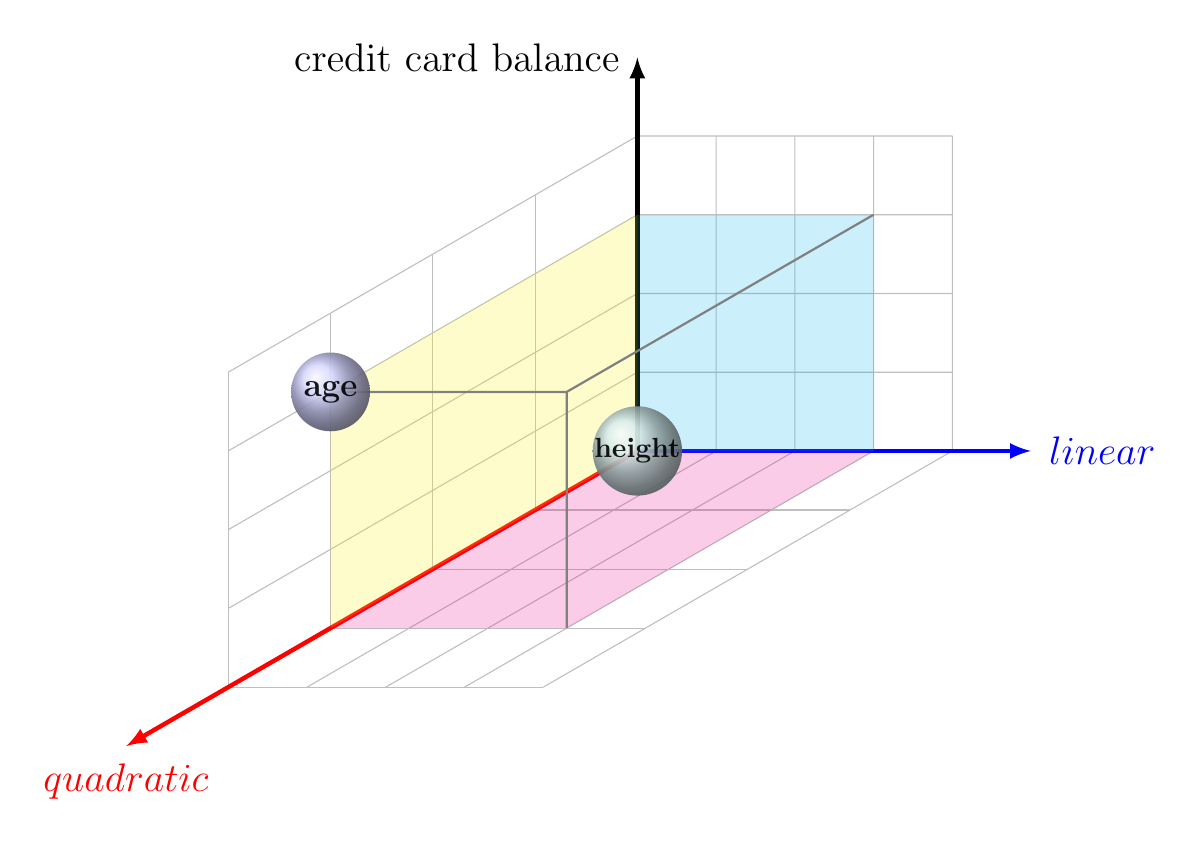
\begin{tikzpicture}[inner sep=0.2cm]
				\def \radi{4}
				\def \x{3}
				\def \y{3}
				\def \z{3}
				
				\begin{scope}[isometricYXZ]
				% the grid
				\begin{scope}[color=gray!50, thin]
				\foreach \xi in {0,...,\radi}{ \draw (\xi,\radi,0) -- (\xi,0,0) -- (\xi,0,\radi); }%
				\foreach \yi in {1,...,\radi}{ \draw (0,\yi,\radi) -- (0,\yi,0) -- (\radi,\yi,0); }%
				\foreach \zi in {0,...,\radi}{ \draw (0,\radi,\zi) -- (0,0,\zi) -- (\radi,0,\zi); }%
				\end{scope}
				
				\draw[-latex, ultra thick, color=blue] (0,0,0) -- (5,0,0) node[anchor=west] {\Large $linear$};%
				\draw[-latex, ultra thick, color=red] (0,0,0) -- (0,5,0) node[anchor=north] {\Large $quadratic$};%
				\draw[-latex, ultra thick, color=black] (0,0,0) -- (0,0,5) node[anchor=east] {\Large credit card balance};%
				
				\fill[color=magenta, opacity=0.2] (0,0,0) -- (\x,0,0) -- (\x,\y,0) -- (0,\y,0) -- cycle; %
				\fill[color=yellow, opacity=0.2] (0,0,0) -- (0,0,\z) -- (0,\y,\z) -- (0,\y,0) -- cycle; %
				\fill[color=cyan, opacity=0.2] (0,0,0) -- (\x,0,0) -- (\x,0,\z) -- (0,0,\z) -- cycle;
				
				\draw[color=gray, thick]%
				(0,\y,\z) -- (\x,\y,\z) -- (\x,\y,0) (\x,\y,\z) -- (\x,0,\z);%
				\end{scope}
				
				%\shade[ball color=yellow] ($\y*(-1.299cm,-0.75cm)+(\x,\z)$) circle (0.1);%
				\node[circle, minimum width=1cm, inner sep=0pt, outer sep=0pt, ball color=blue!20!white,opacity=0.90] (H-1) at ($\y*(-1.299cm,-0.75cm)+(0,\z)$) {\large \bfseries age};
				\node[circle, minimum width=2*\ab cm, inner sep=0pt, outer sep=0pt, ball color=blue!50!green!20!white,opacity=.9] (H-1) at (0,0,0) {\bfseries height};
				\end{tikzpicture}
			}
		}
		\subfloat[Group Lasso \label{fig:2}]{
			\resizebox{200pt}{!}{
				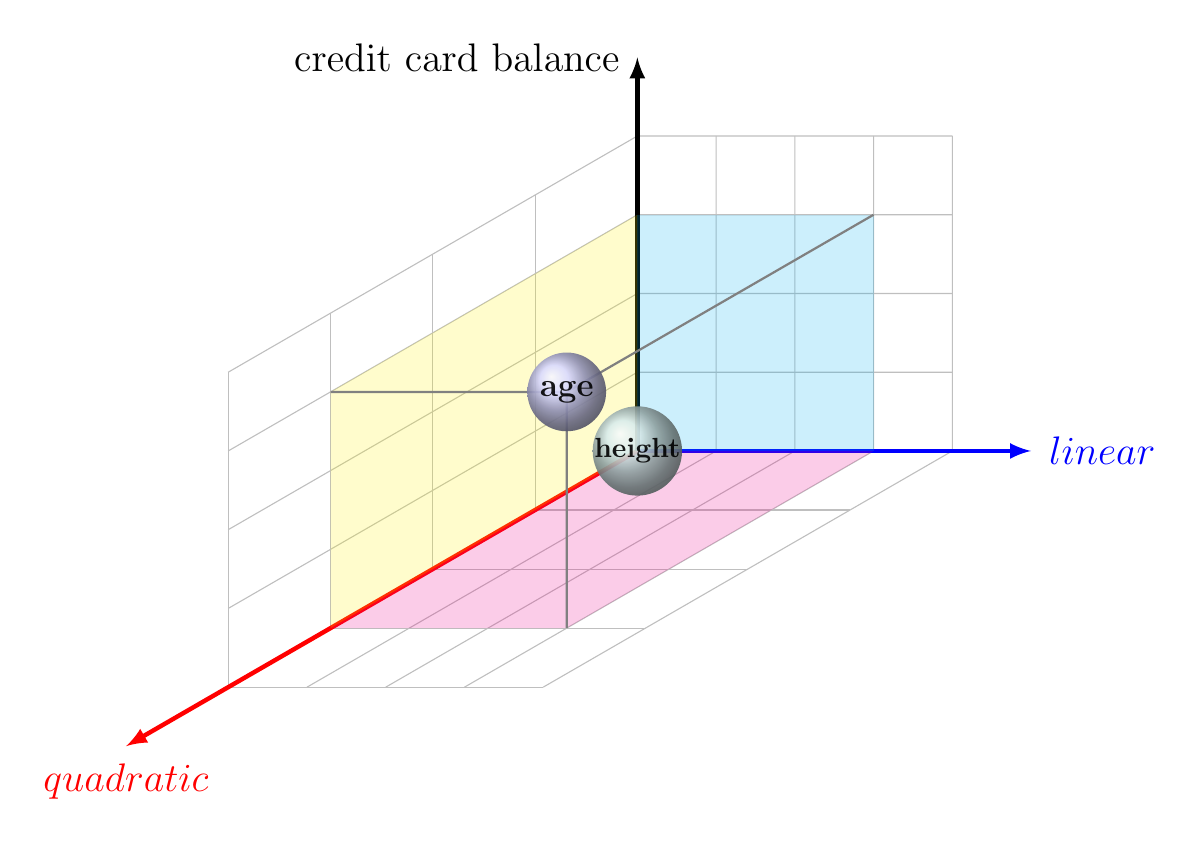
\begin{tikzpicture}[inner sep=0.2cm]
				\def \radi{4}
				\def \x{3}
				\def \y{3}
				\def \z{3}
				
				\begin{scope}[isometricYXZ]
				% the grid
				\begin{scope}[color=gray!50, thin]
				\foreach \xi in {0,...,\radi}{ \draw (\xi,\radi,0) -- (\xi,0,0) -- (\xi,0,\radi); }%
				\foreach \yi in {1,...,\radi}{ \draw (0,\yi,\radi) -- (0,\yi,0) -- (\radi,\yi,0); }%
				\foreach \zi in {0,...,\radi}{ \draw (0,\radi,\zi) -- (0,0,\zi) -- (\radi,0,\zi); }%
				\end{scope}
				
				\draw[-latex, ultra thick, color=blue] (0,0,0) -- (5,0,0) node[anchor=west] {\Large $linear$};%
				\draw[-latex, ultra thick, color=red] (0,0,0) -- (0,5,0) node[anchor=north] {\Large $quadratic$};%
				\draw[-latex, ultra thick, color=black] (0,0,0) -- (0,0,5) node[anchor=east] {\Large credit card balance};%
				
				\fill[color=magenta, opacity=0.2] (0,0,0) -- (\x,0,0) -- (\x,\y,0) -- (0,\y,0) -- cycle; %
				\fill[color=yellow, opacity=0.2] (0,0,0) -- (0,0,\z) -- (0,\y,\z) -- (0,\y,0) -- cycle; %
				\fill[color=cyan, opacity=0.2] (0,0,0) -- (\x,0,0) -- (\x,0,\z) -- (0,0,\z) -- cycle;
				
				\draw[color=gray, thick]%
				(0,\y,\z) -- (\x,\y,\z) -- (\x,\y,0) (\x,\y,\z) -- (\x,0,\z);%
				\end{scope}
				
				%\shade[ball color=yellow] ($\y*(-1.299cm,-0.75cm)+(\x,\z)$) circle (0.1);%
				\node[circle, minimum width=1cm, inner sep=0pt, outer sep=0pt, ball color=blue!20!white,opacity=0.90] (H-1) at ($\y*(-1.299cm,-0.75cm)+(\x,\z)$) {\large \bfseries age};
				\node[circle, minimum width=2*\ab cm, inner sep=0pt, outer sep=0pt, ball color=blue!50!green!20!white,opacity=.9] (H-1) at (0,0,0) {\bfseries height};
				\end{tikzpicture}
			}
			
		}
		\caption{Visualizing the key difference between the lasso and group lasso penalties}\label{fig:lasso_grouplasso_comparison}
\end{figure}


This description follows mainly Yang and Zou (2015). We add the weight matrix.

\subsection{Model}
Only the third term of the log-likelihood~\eqref{eq:loglikrowrank} depends on $\bbeta$:
\begin{equation}
\frac{1}{2} \left\lbrace \left(\bY - \bX\bbeta \right)^T  \left[\frac{1}{\sigma^2(1-\eta)}\left(  \bI_{N_T} - \bU_1 \left(\frac{1-\eta}{\eta}\bSigma_1^{-1} + \bI_{k}\right) ^{-1}\bU_1^T \right)  \right] \left(\bY - \bX\bbeta \right)  \right\rbrace \label{eq:likeW}
\end{equation}
Equation~\eqref{eq:likeW} can be written more generally as
\[
L(\bbeta\mid\bD)=\frac{1}{2}\left[\bY-\widehat{\bY}\right]^{\top}\mathbf{W}\left[\bY-\widehat{\bY}\right]
\]
where $\widehat{\bY}=\sum_{j=1}^{p}\beta_{j}X_{j}$, $\bD$ is the working data $\lbrace \bY, \bX \rbrace$, and $\bW$ is an $N_T \times N_T$ weight matrix given by
\begin{equation}
\bW = \frac{1}{\sigma^2(1-\eta)}\left(  \bI_{N_T} - \bU_1 \left(\frac{1-\eta}{\eta}\bSigma_1^{-1} + \bI_{k}\right) ^{-1}\bU_1^T \right)   \label{eq:weight}
\end{equation}

%Consider the linear regression problem where we have a continuous response $\by\in\mathbb{R}^{n}$
%and let $\bX$ be the design matrix with $n$ rows and $p$ columns where $n$ is the sample size of the raw data. If an intercept is used in the model, we let the first column of $\bX$ be a vector of 1.
Assume that we the predictors in the design matrix $\bX \in \mathbb{R}^{N_T \times p}$ belong to $K$ groups and that the group membership is already defined such that $(1,2,\ldots,p)=\bigcup_{k=1}^{K}I_{k}$ and the cardinality of index set $I_{k}$ is $p_{k}$, $I_{k}\bigcap I_{k^{\prime}}=\emptyset$ for $k\neq k^{\prime},1\le k,k^{\prime}\le K$. Thus group $k$ contains $p_{k}$ predictors, which are $x_{j}$'s for $j\in I_{k}$, and $1\le k\le K.$ If an intercept is included, then $I_{1}=\{1\}$. Given the group partition, we use $\bbeta_{(k)}$ to denote the segment of $\bbeta$ corresponding to group $k$. This notation is used for any $p$-dimensional vector.
%In a more compact form, and introducing observation weights
%\[
%L(\bbeta\mid\bD)=\frac{1}{2}\left[Y-\hat{Y}\right]^{\top}\mathbf{W}\left[Y-\hat{Y}\right]
%\]
%where $\hat{Y}=\sum_{j=1}^{p}\beta_{j}X_{j}$, $\bD$ is the working data $\lbrace \by, \bX \rbrace$, $\bW$ is an $N_T \times N_T$ weight matrix. Then the problem we consider can be expressed as
We consider the group lasso penalized estimator
\begin{equation}
\min_{\bbeta}L(\bbeta \mid \bD)+\lambda\sum_{k=1}^{K}w_{k}\|\bbk\|_{2},\label{eq:wlslasso}
\end{equation}

The loss function $L$ satisfies the quadratic majorization (QM) condition, since there exists
a $p\times p$ matrix $\bH=\bX^{\trans}\mathbf{W}\bX$, and $\nabla L(\bbeta|\bD)=-\left(Y-\hat{Y}\right)^{\top}\mathbf{W}\bX$, which may only depend on the data $\bD$, such that for all $\bbeta,\bbeta^{*}$,
\begin{equation}
L(\bbeta\mid\bD)\le L(\bbeta^{*}\mid\bD)+(\bbeta-\bbeta^{*})^{\trans}\nabla L(\bbeta^{*}|\bD)+\frac{1}{2}(\bbeta-\bbeta^{*})^{\trans}\bH(\bbeta-\bbeta^{*}).\label{QM1}
\end{equation}

\subsection{Algorithm}

Noticing that the penalty term $\sum_{k=1}^{K}w_{k}||\bbeta_{(k)}||_{2}$ is separable with respect to the indices of the features $k=1, \ldots, K$, we can derive the \textit{groupwise-majorization-descent} (GMD) algorithm for computing the solution of~\eqref{eq:wlslasso} when the loss function satisfies the QM condition. Let $\widetilde{\bbeta}$ denote the current solution of $\bbeta$. Without loss of generality, let us derive the GMD update of $\bbkt$, the coefficients of group $k$. Define $\bH_{k}$ as the sub-matrix of $\bH$ corresponding to group $k$. For example, if group 2 is $\{2,4\}$ then $\bH_{(2)}$ is a $2\times2$ matrix with
\[
\bH_{(2)}=\left[\begin{array}{cc}
h_{2,2} & h_{2,4}\\
h_{4,2} & h_{4,4}
\end{array}\right],
\]

where $h_{i,j}$ is the $i,j$th entry of the $\bH$ matrix. Write $\bbeta$ such that $\bbeta_{(k^{\prime})}=\widetilde{\bbeta}_{(k^{\prime})}$ for $k^{\prime}\ne k$. Given $\bbeta_{(k^{\prime})}=\widetilde{\bbeta}_{(k^{\prime})}$ for $k^{\prime}\ne k$, the optimal $\bbk$ is defined as
\begin{equation}
\arg\min_{\boldsymbol{\beta}^{(k)}}L(\bbeta\mid\bD)+\lambda w_{k}\Vert\bbk\Vert_{2}.\label{GMDeq1}
\end{equation}
Unfortunately, there is no closed form solution to~\eqref{GMDeq1} for a general loss function with general design matrix. We overcome the computational obstacle by taking advantage of the QM condition. From~\eqref{QM1} we have
\[
L(\bbeta\mid\bD)\le L(\widetilde{\bbeta}\mid\bD)+(\bbeta-\widetilde{\bbeta})^{\trans}\nabla L(\widetilde{\bbeta}|\bD)+\frac{1}{2}(\bbeta-\widetilde{\bbeta})^{\trans}\bH(\bbeta-\widetilde{\bbeta}).
\]

Write $U(\widetilde{\bbeta})=-\nabla L(\widetilde{\bbeta}|\bD)$. Using
\[
\bbeta-\widetilde{\bbeta}=(\underbrace{0,\ldots,0}_{k-1},\bbk-\bbkt,\underbrace{0,\ldots,0}_{K-k}),
\]
we can write
\begin{equation}
L(\bbeta\mid\bD)\le L(\widetilde{\bbeta}\mid\bD)-(\bbk-\bbkt)^{\trans}U_{(k)}+\frac{1}{2}(\bbk-\bbkt)^{\trans}\bH_{(k)}(\bbk-\bbkt).\label{GMDeq2}
\end{equation}
where
\begin{align}
U_{(k)} & =\frac{\partial}{\partial\bbk}L_{Q}(\bbeta\mid\bD)=-\left(Y-\hat{Y}\right)^{\top}\mathbf{W}\mathbf{X}_{(k)},\label{eq:gradientj-1}\\
\mathbf{H}_{(k)} & =\frac{\partial^{2}}{\partial\bbk\partial\bbk^{\top}}L_{Q}(\bbeta\mid\bD)=\mathbf{X}_{(k)}^{\top}\mathbf{W}\mathbf{X}_{(k)}.\label{eq:hessianj-1}
\end{align}

Let $\eta_{k}$ be the largest eigenvalue of $\bH_{(k)}$. We set $\gamma_{k}=(1+\varepsilon^{*})\eta_{k}$, where $\varepsilon^{*}=10^{-6}$. Then we can further relax the upper bound in~\eqref{GMDeq2} as
\begin{equation}
L(\bbeta\mid\bD)\leq L(\widetilde{\bbeta}\mid\bD)-(\bbeta^{(k)}-\widetilde{\bbeta}^{(k)})^{\trans}U_{(k)}+\frac{1}{2}\gamma_{k}(\bbeta^{(k)}-\widetilde{\bbeta}^{(k)})^{\trans}(\bbeta^{(k)}-\widetilde{\bbeta}^{(k)}).\label{GMDeq3-1}
\end{equation}
It is important to note that the inequality strictly holds unless for $\bbeta^{(k)}=\widetilde{\bbeta}^{(k)}$. Instead of minimizing~\eqref{GMDeq1} we solve
\begin{equation}
\arg\min_{\bbeta^{(k)}}L(\widetilde{\bbeta}\mid\bD)-(\bbeta^{(k)}-\widetilde{\bbeta}^{(k)})^{\trans}U_{(k)}+\frac{1}{2}\gamma_{k}(\bbeta^{(k)}-\widetilde{\bbeta}^{(k)})^{\trans}(\bbeta^{(k)}-\widetilde{\bbeta}^{(k)})+\lambda w_{k}\Vert\bbeta^{(k)}\Vert_{2}.\label{GMDeq4-1}
\end{equation}

Denote by $\widetilde{\bbeta}^{(k)}(\textrm{new})$ the solution to~\eqref{GMDeq4-1}. It is straightforward to see that $\widetilde{\bbeta}^{(k)}(\textrm{new})$ has a simple closed-from expression
\begin{equation}
\widetilde{\bbeta}^{(k)}(\textrm{new})=\frac{1}{\gamma_{k}}\left(U^{(k)}+\gamma_{k}\widetilde{\bbeta}^{(k)}\right)\left(1-\frac{\lambda w_{k}}{\Vert U^{(k)}+\gamma_{k}\widetilde{\bbeta}^{(k)}\Vert_{2}}\right)_{+}.\label{GMDeq5-1}
\end{equation}

Algorithm~\ref{alg1} summarizes the details of GMD.

\begin{algorithm}
	\begin{enumerate}
		\item For $k=1,\ldots,K$, compute $\gamma_k$, the largest eigenvalue of $\bH^{(k)}$.
		\item Initialize $\widetilde \bbeta$.
		\item Repeat the following cyclic groupwise updates until convergence:
		\begin{enumerate}
			\item[---] for $k=1,\ldots,K$, do step (3.1)--(3.3)
			\begin{enumerate}
				\item[3.1]
				Compute $U(\widetilde \bbeta )=-\nabla L(\widetilde \bbeta | \bD)$.
				\item[3.2]
				Compute
				$
				\widetilde \bbeta^{(k)}(\textrm{new}) = \frac{1}{\gamma_k}\left( U^{(k)}+\gamma_k \widetilde \bbeta^{(k)} \right)\left(1-\frac{\lambda w_k}{\Vert U^{(k)}+\gamma_k \widetilde \bbeta^{(k)} \Vert_2}\right)_{+} .
				$
				\item[3.3]
				Set $\widetilde \bbeta^{(k)}=\widetilde \bbeta^{(k)}(\textrm{new})$.
			\end{enumerate}
		\end{enumerate}
	\end{enumerate}
	\caption{The GMD algorithm for general group-lasso learning. \label{alg1}}
\end{algorithm}


\subsection{Convergence}

We can prove the strict descent property of GMD by using the MM principle \citep{MM1,hunter2004tutorial,MM08}. Define
\begin{equation}
Q(\bbeta \mid \bD)=L(\widetilde \bbeta \mid \bD)-(\bbeta^{(k)}-\widetilde \bbeta^{(k)})^{\trans}
U^{(k)}+\frac{1}{2} \gamma_k (\bbeta^{(k)}-\widetilde \bbeta^{(k)})^{\trans} ( \bbeta^{(k)}- \widetilde \bbeta^{(k)})+\lambda w_k \Vert \bbeta^{(k)}\Vert_2.
\end{equation}
Obviously, $Q(\bbeta \mid \bD)=L(\bbeta \mid \bD)+\lambda w_k \Vert \bbeta^{(k)}\Vert_2$ when $\bbeta^{(k)}=\widetilde \bbeta^{(k)}$ and
(\ref{GMDeq3}) shows that
$Q(\bbeta \mid \bD) > L(\bbeta \mid \bD)+\lambda w_k \Vert \bbeta^{(k)}\Vert_2$ when $\bbeta^{(k)} \neq \widetilde \bbeta^{(k)}$.
After updating $\widetilde \bbeta^{(k)}$ using (\ref{GMDeq5}), we have
\begin{eqnarray*}
	L(\widetilde \bbeta^{(k)}(\textrm{new}) \mid \bD)+\lambda w_k \Vert \widetilde \bbeta^{(k)}(\textrm{new}) \Vert_2
	&  \le &  Q(\widetilde \bbeta^{(k)}(\textrm{new})  \mid \bD)\\
	& \le & Q(\widetilde \bbeta  \mid \bD) \\
	& = & L(\widetilde \bbeta \mid \bD)+\lambda w_k \Vert \widetilde \bbeta^{(k)}\Vert_2.
\end{eqnarray*}
Moreover, if $\widetilde \bbeta^{(k)}(\textrm{new}) \neq \widetilde \bbeta^{(k)}$, then the first inequality becomes
\begin{eqnarray*}
	L(\widetilde \bbeta^{(k)}(\textrm{new}) \mid \bD)+\lambda w_k \Vert \widetilde \bbeta^{(k)}(\textrm{new}) \Vert_2
	&  < &  Q(\widetilde \bbeta^{(k)}(\textrm{new})  \mid \bD).
\end{eqnarray*}
Therefore, the objective function is strictly decreased after updating all groups in a cycle, unless the solution does not change after each groupwise update. If this is the case,
we can show that the solution must satisfy the KKT conditions, which means that the algorithm converges and finds the right answer. To see this,
if $\widetilde \bbeta^{(k)}(\textrm{new}) = \widetilde \bbeta^{(k)}$ for all $k$, then by the update formula \eqref{GMDeq5-1} we have that for all $k$
\begin{align}\label{KKTcond1}
\widetilde \bbeta^{(k)} = \frac{1}{\gamma_k}\left( U^{(k)}+\gamma_k \widetilde \bbeta^{(k)} \right)\left(1-\frac{\lambda w_k}{\Vert U^{(k)}+\gamma_k \widetilde \bbeta^{(k)} \Vert_2}\right) \qquad\textrm{if }\Vert U^{(k)}+\gamma_k \widetilde \bbeta^{(k)} \Vert_2 > \lambda w_{k},\\\label{KKTcond2}
\widetilde \bbeta^{(k)} = \boldsymbol{0} \qquad\textrm{if }\Vert U^{(k)}+\gamma_k \widetilde \bbeta^{(k)} \Vert_2 \leq \lambda w_{k}.
\end{align}
By straightforward algebra  we obtain the KKT conditions:
\begin{align*}
-U^{(k)}+\lambda w_{k}\cdot\frac {\widetilde\bbeta^{(k)} }{\Vert\widetilde\bbeta^{(k)}\Vert_2}=\boldsymbol{0}\qquad\textrm{if }\widetilde\bbeta^{(k)}\neq \boldsymbol{0},\\
\left\Vert
U^{(k)}
\right\Vert_2 \le\lambda w_{k}\qquad\textrm{if }\widetilde\bbeta^{(k)}=\boldsymbol{0},
\end{align*}
where $k=1,2,\ldots,K$. Therefore, if the objective function stays unchanged after a cycle, the algorithm necessarily converges to the right
answer.




\section{Penalized interaction models}


%In the context of studying gene environment interactions, all previously mentioned methods can yield results where the main effects are 0 but the cross terms are not. While there may exist situations where this can occur, such behavior is generally not biologically plausible in genomics~\citep{bakermans2015hidden}. 
%Two other arguments against such behavior have to do with statistical power and practical importance; 1) large main effects are more likely to lead to detectable interactions than small ones~\citep{cox1984interaction} and 2) a data collector cares about the number of variables they need to \textit{measure} to make predictions at a future time~\citep{bien2013lasso}. 
%Moreover, the proposed clustering methods are based on features from all observations. Any correlation patterns specific to a subgroup of patients (e.g. Figures~\ref{fig:COPDnevercorr} and~\ref{fig:COPDcurrentcorr}) may become diluted when looking at the overall correlation matrix. 
%Therefore the focus of my doctoral research will be on developing a method that can identify previously unknown sets of highly correlated genes that interact with the environment to explain phenotypic variation, with a focus on prediction accuracy and model interpretability. 

Then something about other structured L1 penalizations that have been proposed. There are quite a few examples of penalties built for specific applications, and maybe you could find a few such examples and cite them. Not comprehensively.  Then you can point to the sail chapter as a new structured penalty.

\ctable[pos=H,doinside=\footnotesize]{lcc}{
}{
\FL
Type      & Method   & Software \ML
\multicolumn{1}{m{1cm}}{Linear}    & \multicolumn{1}{m{6cm}}{\texttt{CAP}~\citep{zhao2009composite} }        &   \xmark    \\
& \multicolumn{1}{m{4cm}}{\texttt{SHIM}~\citep{choi2010variable}}        &   \xmark    \\
& \multicolumn{1}{m{4cm}}{\texttt{hiernet}~\citep{bien2013lasso}}        &   \texttt{hierNet(x, y)}    \\
& \multicolumn{1}{m{4cm}}{\texttt{GRESH}~\citep{she2014group} }        &  \xmark     \\
& \multicolumn{1}{m{4cm}}{\texttt{FAMILY}~\citep{haris2016convex}}    &  \texttt{FAMILY(x, z, y)}   \\
& \multicolumn{1}{m{4cm}}{\texttt{glinternet}~\citep{lim2015learning} }    & \texttt{glinternet(x, y)}  \\			   	 	
& \multicolumn{1}{m{4cm}}{\texttt{RAMP}~\citep{hao2018model}}        & \texttt{RAMP(x, y)}  \\ 
& \multicolumn{1}{m{4cm}}{\texttt{LassoBacktracking}~\citep{shah2016modelling}   }        & \texttt{LassoBT(x, y)}  \ML
\multicolumn{1}{m{4cm}}{Non-linear} 	& \multicolumn{1}{m{8cm}}{\texttt{VANISH}~\citep{radchenko2010variable} }        & \xmark  \\
& \multicolumn{1}{m{4cm}}{\texttt{sail}}        & \texttt{sail(x, y, e)}  \LL
}

\subsection{Current methods overview and their limitations} \label{subsec:methods-overview2}

We consider a regression model for an outcome variable $Y=(y_1, \ldots, y_n)$ which follows an exponential family. Let $E=(e_1, \ldots, e_n)$ be the binary environment vector and $\bx = (X_{1}, \ldots, X_{p})$ be the matrix of high-dimensional data. Consider the regression model with main effects and their interactions with $E$:
\begin{align}
g(\bmu)  = & \beta_0  + \underbrace{\beta_1 X_{1} + \cdots + \beta_p X_p + \beta_{E} E}_{\tm{main effects}} + \underbrace{\alpha_{1E} (X_1 E) + \cdots + \alpha_{pE} (X_p E)}_{\tm{interactions}} \label{eq:linpred1}
\end{align}
where $g(\cdot)$ is a known link function and $\bmu = \e\left[Y|\bx, E, \bbeta,\balpha\right]$. Our goal is to estimate the parameters \mbox{$\bbeta = \left(\beta_1, \beta_2, \ldots, \beta_p, \beta_E\right) \in \mathbb{R}^{p+1}$} and $\boldsymbol{\alpha} = \left(\alpha_{1E}, \ldots, \alpha_{pE}\right) \in \mathbb{R}^p$ and to improve prediction of $Y$. In fact, in the light of our goals to improve prediction and interpretability, we also consider the related model
\begin{equation}  g(\bmu) = \beta^*_0 + \sum_{k=1}^q \beta^*_k \widetilde{X}_k + \beta^*_E E + 
\sum_{k=1}^q \alpha^*_k E \widetilde{X}_k 
\label{eq:linpred1.1}
\end{equation}
where $\widetilde{X}_k, k=1, \ldots, q$ are linear combinations of $X$ designed to reduce the dimension, such that $q<<p$, and the superscript asterisk on the parameters is just to emphasize that these are different from those in~\eqref{eq:linpred1}. In what follows, we omit the asterisk on the parameters for clarity.


\subsection{Phase 3: Variable Selection} \label{sec:varselect}
%Because the clustering in phase 1 is unsupervised, it is possible that the derived latent representations from phase 2 will not be associated with the response. Therefore we propose to regress the response on the summary measures via penalized likelihood of the form given by \ref{eq:penalisedlikelihood}. These methods are able to simultaneous estimate and select regression parameters. We argue that the selected non-zero predictors in this model will represent clusters of genes that interact with the environment and are associated with the phenotype. Such an additive model might be insufficient for predicting the outcome. In this case we may directly include the environment variable, the summary measures and their interaction. However, since no constraint is placed on the structure of the model in~\ref{eq:penalisedlikelihood}, it is possible that the estimated main effects are zero while the interaction term is not. This has motivated methods that produce structured sparsity~\cite{bach2012structured}. For example, Bien \textit{et al.}~\cite{bien2013lasso} propose a strong hierarchical lasso which forces the main effects to be included if the interaction term is non-zero. However this method and related ones are restricted to all pairwise interactions between $p$ measured variables. Therefore I will explore methods that impose a strong hierarchy in the context of gene environment interactions. 
We are interested in imposing the strong heredity principle~\citep{chipman1996bayesian}: 
\begin{equation}
\hat{\alpha}_{jE} \neq 0 \qquad \Rightarrow \qquad \hat{\beta}_j \neq 0 \qquad \tm{and} \qquad \hat{\beta}_E \neq 0   \label{eq:heredity}
\end{equation}
In words, the interaction term will only have a non-zero estimate if its corresponding main effects are estimated to be non-zero. One benefit brought by hierarchy is that the number of measured variables can be reduced, referred to as practical sparsity~\cite{she2014group,bien2013lasso}. For example, a model involving $X_1, E, X_1 \cdot E$ is more parsimonious than a model involving $X_1, E, X_2 \cdot E$, because in the first model a researcher would only have to measure two variables compared to three in the second model. In order to address these issues, we propose to extend the model of Choi \textit{et al.}~\citep{choi2010variable} to simultaneously perform variable selection, estimation and impose the strong heredity principle in the context of high dimensional interactions with the environment (HD$\times E$). To do so, we follow Choi and reparametrize the coefficients for the interaction terms as $\alpha_{jE} = \gamma_{jE} \beta_j \beta_E$. Plugging this into~\eqref{eq:linpred1}:
\begin{align}
g(\bmu)  = & \beta_0  + \beta_1 \widetilde{X}_{1} + \cdots + \beta_q \widetilde{X}_q + \beta_{E} E + \gamma_{1E}\beta_1 \beta_E (\widetilde{X}_1 E) + \cdots + \gamma_{qE}\beta_q \beta_E (\widetilde{X}_q E)    \label{eq:linpred2}
\end{align}
where $\widetilde{\bx} = (\widetilde{X}_1, \ldots, \widetilde{X}_q)$ are the cluster representatives derived in phase 2 and $q <p$. This reparametrization directly enforces the strong heredity principle (Eq.~\eqref{eq:heredity}), i.e., if either main effect estimates are 0, then $\hat{\alpha}_{jE}$ will be zero and a non-zero interaction coefficient implies non-zero $\hat{\beta}_j$ and $\hat{\beta}_E$. To perform variable selection in this new parametrization, we follow Choi \textit{et al.}~\cite{choi2010variable} and penalize $\bs{\gamma} = \left(\gamma_{1E}, \ldots, \gamma_{pE}\right)$ instead of penalizing $\balpha$ as in~\eqref{eq:lassolikelihood}, leading to the following penalized least squares criterion:
\begin{equation}
\argmin_{\beta_0, \bbeta, \bs{\gamma} }  \frac{1}{2} \norm{Y - g(\bmu)}^2 + \lambda_\beta \left(w_1 \beta_1 + \cdots + w_q \beta_q + w_E \beta_E   \right) + \lambda_\gamma  \left( w_{1E} \gamma_{1E} + \cdots + w_{qE}\gamma_{qE}         \right) \label{eq:lassolikelihood2}
\end{equation} 
where $g(\bmu)$ is from~\eqref{eq:linpred2}, $\lambda_\beta$ and $\lambda_\gamma$ are tuning parameters and $\mb{w} = \left(w_{1}, \ldots, w_q, w_{1E}, \ldots, w_{qE}\right)$ are prespecified adaptive weights. The $\lambda_\beta$ tuning parameter controls the amount of shrinkage applied to the main effects, while $\lambda_\gamma$ controls the interaction estimates and allows for the possibility of excluding the interaction term from the model even if the corresponding main effects are non-zero. The adaptive weights serve as a way of allowing parameters to be penalized differently. Furthermore, adaptive weighting~\citep{zou2006adaptive} has been shown to construct oracle procedures~\citep{fan2001variable}, i.e., asymptotically, it performs as well as if the true model were given in advance. The oracle property is achieved when the weights are a function of any root-$n$ consistent estimator of the true parameters e.g. maximum likelihood (MLE) or ridge regression estimates. It can be shown that the procedure in~\eqref{eq:lassolikelihood2} asymptotically possesses the oracle property~\citep{choi2010variable}, even when the number of parameters tends to $\infty$ as the sample size increases, if the weights are chosen such that
\begin{equation}
w_j = \left | \frac{1}{\hat{\beta}_j} \right|, \quad w_{jE} = \left | \frac{\hat{\beta}_j \hat{\beta}_E}{\hat{\alpha}_{jE}} \right| \quad \tm{ for }j=1, \ldots, q   \label{eq:weights}
\end{equation}
where $\hat{\beta}_j$ and $\hat{\alpha}_{j}$ are the MLEs, \textit{using the transformed variables}, from~\eqref{eq:linpred1} or the ridge regression estimates when $q > n$. The rationale behind the data-dependent $\hat{\bs{w}}$ is that as the sample size grows, the weights for the truly zero predictors go to $\infty$ (which translates to a large penalty), whereas the weights for the truly non-zero predictors converge to a finite constant~\citep{zou2006adaptive}. 

There have been several more recent proposals for modeling interactions with the strong heredity constraint in the variable selection via penalization literature including Composite Absolute Penalties (CAP)~\citep{zhao2009composite}, Variable selection using Adaptive Nonlinear Interaction Structures in High dimensions (VANISH)~\citep{radchenko2010variable}, Strong Hierarchical Lasso (hierNet)~\citep{bien2013lasso}, Group-Lasso Interaction Network (glinternet)~\citep{lim2015learning}, Group Regularized Estimation under Structural Hierarchy (GRESH)~\citep{she2014group} and a Framework for Modeling Interactions with a Convex Penalty (FAMILY)~\citep{haris2014convex}. While each method has their own merit, including that they are all convex optimization problems, they all contain complex penalty functions which are hard to interpret and lead to computationally expensive fitting algorithms. On the other hand, the objective function in~\eqref{eq:lassolikelihood2} can be solved using an iterative approach (by first fixing $\bbeta$ and then $\balpha$) which simplifies to a LASSO type problem; one that has been extensively studied, is well understood and can be solved efficiently using existing software (e.g. \texttt{glmnet}~\citep{friedman2010regularization}). A limitation of this approach is that the optimization problem is non-convex, arising from the reparametrization of $\balpha$ as a product of optimization variables $(\bbeta, \bs{\gamma})$, and hence convergence to the global minimum is not guaranteed~\citep{choi2010variable}. We argue that since there is only one $E$, and that $\widetilde{X}$ is much smaller in dimension, finding a solution is much more likely. 

%We argue here that in our applications, we are more concerned with identifying the truly associated parameters (as given by an oracle procedure) than finding a global minimum which would be guaranteed in a convex formulation. 

To our knowledge, strong hierarchies have never previously been used in HD interaction analysis in genomics or brain imaging studies. Furthermore, the specific choices of weights proposed here, i.e., based on the transformed variables from phase 2, have not been previously used. Choi \textit{et al.}~\citep{choi2010variable} estimated their weights simultaneously, but this would not be feasible in HD data. Finally, the adaptation to interactions with one key $E$ variable is specific to our situation and this leads to computational efficiencies. These three points constitute novel aspects of this thesis. I have a working implementation of this, and am in the process of conducting simulation studies.


\section{Penalized linear mixed models}
(5) A brief intro to linear mixed models followed by why naive penalization violates the normality of residuals to motivate your ggmix chapter.


%\section{you will need a section on things like gradient descent and other algorithms for finding solutions efficiently}
	%-----------------------------------------------------------------------------
\chapter{Sparse Additive Interaction Learning\label{ch:sail}}
%-----------------------------------------------------------------------------

Sahir Rai Bhatnagar$^{1,2}$, Amanda Lovato$^{2}$, Yi Yang$^{3}$, Celia MT Greenwood$^{1,2}$
%\affil[1]{Department of Epidemiology, Biostatistics and Occupational Health, McGill University}
%\affil[2]{Lady Davis Institute, Jewish General Hospital, Montr\'{e}al, QC}
%\affil[3]{Departments of Oncology and Human Genetics, McGill University}
%\affil[4]{Department of Mathematics and Statistics, McGill University}
%\affil[5]{Montreal Neurological Institute, McGill University}
%\affil[6]{Department of Computer Science, McGill University}
%\affil[7]{Department of Biochemistry, Universit\'{e} de Sherbrooke}

%\author{Brian D. Beitzel}
$^{1}$Department of Epidemiology, Biostatistics and Occupational Health, McGill University\\
$^{2}$Lady Davis Institute, Jewish General Hospital, Montr\'{e}al, QC \\
$^{3}$Department of Mathematics and Statistics, McGill University\\



\newpage

\section*{Abstract}
Diseases are now thought to be the result of changes in entire biological networks whose states are affected by a complex interaction of genetic and environmental factors. In general, power to estimate interactions is low, the number of possible interactions could be enormous and their effects may be non-linear. Existing approaches such as the lasso might keep an interaction but remove a main effect, which is problematic for interpretation. We develop a model for linear and non-linear interactions in penalized regression models that automatically enforces the strong heredity property. A computationally efficient fitting algorithm combined with a non-parametric screening approach scales to high-dimensional datasets and has been implemented in an R package. We apply our method to identify gene-prenatal maternal depression interactions on negative emotionality in mother–infant dyads from the Maternal Adversity, Vulnerability, and Neurodevelopment (MAVAN) cohort.

\newpage

\section{Introduction}

Computational approaches to variable selection have become increasingly important with the advent of high-throughput technologies in genomics and brain imaging studies, where the data has become massive, yet where it is believed that the number of truly important variables is small relative to the total number of variables. 
Although many approaches have been developed for main effects, there is an enduring interest in powerful methods for estimating interactions, since interactions may reflect important modulation of a genomic system by an external factor~\citep{bhatnagar2018analytic}. 
Accurate capture of interactions may hold the potential to better understanding  biological phenomena and improving prediction accuracy. 
For example, a model that considered interactions between brain imaging data and genetic features had better classification accuracy compared to a model that considered the main effects only~\citep{ning2018classifying}. 
%For example, genome wide association studies (GWAS) have been unable to explain a large proportion of heritability (the variance in phenotype attributable to genetic variants) and it has been suggested that this missing heritability may in part be due to gene-environment interactions~\citep{manolio2009finding}. 
Furthermore, the manifestations of disease are often considered to be the result of changes in entire biological networks whose states are affected by a complex interaction of genetic and environmental factors~\citep{schadt2009molecular}. 
However, there is a general deficit of such replicated interactions in the literature~\citep{timpson2018genetic}.   
Indeed, power to detect interactions is always lower than for  main effects, and in high-dimensional settings ($p >> n$), this lack of power to detect interactions is exacerbated, since the number of possible interactions could be enormous and their effects may be non-linear. Hence, analytic methods that may improve power are essential.  

%{\color{green} You need a non-genetic example - i.e. gene expression or proteomic or ...}
Interactions may occur in numerous types and of varying complexities. In this paper, we consider one specific type of interaction models, where one (exposure) variable is involved in possibly non-linear interactions with a high-dimensional set of measures $\mb{X}$ leading to effects on a response variable, $Y$. We propose a multivariable penalization procedure for detecting non-linear interactions $\mb{X}$ and $E$. 


%Our approach improves on existing procedures for detecting such interactions in three ways; 1) it automatically enforces the strong heredity property, i.e., an interaction term can only be included in the model if the corresponding main effects are in the model 2) it reduces the dimensionality of the problem and leverages the high correlations by transforming the input feature space using network connectivity measures and 3) it leads to interpretable models which are biologically meaningful.


%Furthermore, diseases are now thought to be the result of entire biological networks whose states are affected by environmental factors, and these systemic changes can induce or eliminate strong correlations between elements in a network. Therefore, we propose a multivariate penalization procedure for detecting interactions between high dimensional data ($p >> n$) and an environmental factor, where the effect of this environmental factor on the high dimensional data is widespread and plays a role in predicting the response. Our approach improves on existing procedures for detecting such interactions in three ways; 1) it automatically enforces the strong heredity property, i.e., an interaction term can only be included in the model if the corresponding main effects are in the model 2) it reduces the dimensionality of the problem and leverages the high correlations by transforming the input feature space using network connectivity measures and 3) it leads to interpretable models which are biologically meaningful. This thesis is motivated by three studies; one that looks at the impact of maternal care on child development, another that characterizes normal brain development as a function of intelligence scores and one that looks at the long-lasting effects of diet in subsequent generations.


%Diseases are now thought to be the result of changes in entire biological networks whose states are affected by a complex interaction of genetic and environmental factors. In general, power to estimate interactions is low, the number of possible interactions could be enormous and their effects may be non-linear. Existing approaches such as the lasso might keep an interaction but remove a main effect, which is problematic for interpretation. We develop a model for linear and non-linear interactions in penalized regression models that automatically enforces the strong heredity property. A computationally efficient fitting algorithm combined with a non-parametric screening approach scales to high-dimensional datasets and has been implemented in an R package. We apply our method to identify gene-prenatal maternal depression interactions on negative emotionality in mother–infant dyads from the Maternal Adversity, Vulnerability, and Neurodevelopment (MAVAN) cohort.



\subsection{A Sparse additive interaction model}
Let $Y=(Y_1, \ldots, Y_n) \in \mathbb{R}^n$ be a continuous outcome variable, \mbox{$X_E=(E_1, \ldots, E_n) \in \mathbb{R}^n$} a binary or continuous environment vector, and \mbox{$\bX = (X_{1}, \ldots, X_{p}) \in \mathbb{R}^{n\times p}$} a matrix of predictors, possibly high-dimensional. Furthermore let $f_j: \mathbb{R} \rightarrow \mathbb{R}$ be a smoothing method for variable $X_j$ by a projection on to a set of basis functions:
\begin{equation}
f_j(X_j) = \sum_{\ell = 1}^{m_j} \psi_{j\ell}(X_j) \beta_{j\ell} \label{eq:smooth}
\end{equation}
Here, the $\left\lbrace \psi_{j\ell} \right\rbrace_1^{m_j}$ are a family of basis functions in $X_j$~\citep{hastie2015statistical}. Let $\bPsi_j$ be the $n \times m_j$ matrix of evaluations of the $\psi_{j\ell}$ and \mbox{$\btheta_j = (\beta_{j1}, \ldots, \beta_{jm_j}) \in \mathbb{R}^{m_j}$} for $j = 1, \ldots, p$ ($\btheta_j$ is a $m_j$-dimensional column vector of basis coefficients for the $j$th main effect). In this article we consider an additive interaction regression model of the form 
\begin{align}
g(\bmu)  & =  \beta_0 \cdot \boldsymbol{1} + \sum_{j=1}^p \bPsi_j \btheta_j + \beta_E X_E + \sum_{j=1}^p (X_E \circ \bPsi_j) \btau_{j}    \label{eq:linpred}
\end{align}
where $g(\cdot)$ is a known link function, $\bmu = \e\left[Y|\bPsi, X_E \right]$, $\beta_0$ is the intercept, $\beta_E$ is the coefficient for the environment variable, $\btau_j = (\tau_{j1}, \ldots, \tau_{jm_j})\in \mathbb{R}^{m_j}$ are the basis coefficients for the $j$th interaction term, and $(X_E \circ \bPsi_j)$ is the $n \times m_j$ matrix formed by the component-wise multiplication of the column vector $X_E$ by each column of $\bPsi_j$. For a continuous response, we use the squared-error loss to estimate the parameters:
\begin{equation}
\mathcal{L}(\bTheta| \bD) = \frac{1}{2n}\norm{Y - \beta_0 \cdot \boldsymbol{1} - \sum_{j=1}^p \bPsi_j \btheta_j - \beta_E X_E - \sum_{j=1}^p (X_E \circ \bPsi_j) \btau_j }_2^2
\end{equation}
and for binary response $Y_i \in \left\lbrace -1, +1 \right\rbrace$ we use the logistic loss:
\begin{equation}
\mathcal{L}(\bTheta| \bD) = \frac{1}{n} \sum_i \log \left(1 + \exp \left\lbrace - Y_i \left( \beta_0 \cdot \boldsymbol{1} - \sum_{j=1}^p \bPsi_j \btheta_j - \beta_E X_E - \sum_{j=1}^p (X_E \circ \bPsi_j) \btau_j \right) \right\rbrace   \right)
\end{equation}

where $\bTheta \coloneqq (\beta_0, \beta_E,\btheta_1, \ldots, \btheta_p, \btau_1, \ldots, \btau_p)$ and $\bD \coloneqq (Y,\bPsi,X_E)$ is the working data. Here we assume that $p$ is large relative to $n$, and particularly that $\sum_{j=1}^{p}m_j / n$ is large.
Due to the large number of parameters to estimate with respect to the number of observations, one commonly-used approach is to shrink the regression coefficients by placing a constraint on the values
of $(\beta_E, \btheta_j, \btau_j)$. Certain constraints have the added benefit of producing a sparse model in the sense that many of the coefficients will be set exactly to 0~\citep{buhlmann2011statistics}. Such a reduced predictor set can lead to a more interpretable model with smaller prediction variance, albeit at the cost of having biased parameter estimates~\citep{fan2014challenges}. In light of these goals, we consider the following objective function:
\begin{equation}
\argmin_{\bTheta }  	\mathcal{L}(\bTheta| \bD) + \lambda (1-\alpha)  \left( w_E \abs{\beta_E} + \sum_{j=1}^{p} w_j \norm{\btheta_j}_2 \right) +  \lambda\alpha \sum_{j=1}^{p} w_{jE} \norm{\btau_{j}}_2 \label{eq:lassolikelihood3}
\end{equation} 
where $\norm{\btheta_j}_2 = \sqrt{\sum_{k=1}^{m_j} \beta_{jk}^2}$, $\norm{\btau_j}_2 = \sqrt{\sum_{k=1}^{m_j} \tau_{jk}^2}$, $\lambda >0$ and $\alpha \in (0,1)$ are adjustable tuning parameters, $w_E, w_j, w_{jE}$ are non-negative penalty factors for $j=1, \ldots, p$ which serve as a way of allowing parameters to be penalized differently. The first term in the penalty penalizes the main effects while the second term penalizes the interactions. The parameter $\alpha$ controls the relative weight on the two penalties. Note that we do not penalize the intercept. 

An issue with~\eqref{eq:lassolikelihood3} is that since no constraint is placed on the structure of the model, it is possible that an estimated interaction term is nonzero while the corresponding main effects are zero. While there may be certain situations where this is plausible, statisticians have generally argued that interactions should only be included if the corresponding main effects are also in the model~\citep{mccullagh1989generalized}. This is known as the strong heredity principle~\citep{chipman1996bayesian}. Indeed, large main effects are more likely to lead to detectable interactions~\citep{cox1984interaction}. In the next section we discuss how a simple reparametrization of the model~\eqref{eq:lassolikelihood3} can lead to this desirable property. 
%Furthermore, adaptive weighting~\citep{zou2006adaptive} has been shown to construct oracle procedures~\citep{fan2001variable}, i.e., asymptotically, it performs as well as if the true model were given in advance. These weights are given by
%\begin{equation}
%	w_E = \left|   \frac{1}{\hat{\beta}_E} \right| ,\quad w_j = \frac{1}{\norm{\hat{\btheta}_j}_2} , \quad w_{jE} = \left | \frac{\hat{\beta}_E \norm{\hat{\btheta}_j}_2}{\norm{\hat{\alpha}_{j}}_2} \right| \quad \tm{ for }j=1, \ldots, p   \label{eq:weights}
%\end{equation}
%where $\hat{\beta}_E$, $\hat{\btheta}_j$ and $\hat{\balpha}_{j}$ are the MLEs, from~\eqref{eq:linpred} or the ridge regression estimates when $p > n$.

\subsection{Strong and weak heredity}

The strong heredity principle states that an interaction term can only have a non-zero estimate if its corresponding main effects are estimated to be non-zero. The weak heredity principle allows for a non-zero interaction estimate as long as one of the corresponding main effects is estimated to be non-zero~\citep{chipman1996bayesian}. In the context of penalized regression methods, these principles can be formulated as structured sparsity \citep{bach2012structured} problems. Several authors have proposed to modify the type of penalty in order to achieve the heredity principle~\citep{radchenko2010variable,bien2013lasso,haris2014convex,lim2014learning}. We take an alternative approach. Following Choi et al.~\citep{choi2010variable}, we introduce a new set of parameters $\bgamma = (\gamma_1, \ldots, \gamma_p)\in \mathbb{R}^p$ and reparametrize the coefficients for the interaction terms $\btau_j$ in~\eqref{eq:linpred} as a function of $\gamma_j$ and the main effect parameters $\btheta_j$ and $\beta_E$. This reparametrization for both strong and weak heredity is summarized in Table~\ref{tab:reparam}.

\ctable[caption={Reparametrization for strong and weak heredity principle for \texttt{sail} model},label=tab:reparam,pos=h!,doinside=\footnotesize, ]{lll}{
}{
\FL
Type      & Feature  & Reparametrization \ML
\multicolumn{1}{m{3cm}}{Strong heredity}    & \multicolumn{1}{m{5cm}}{$\hat{\btau}_{j} \neq 0 \Rightarrow  \hat{\btheta}_j \neq 0  \tm{ and }  \hat{\beta}_E \neq 0$}        &   $\btau_{j} = \gamma_{j} \beta_E \btheta_j $    \\
\multicolumn{1}{m{3cm}}{Weak heredity} & \multicolumn{1}{m{5cm}}{$\hat{\btau}_{j} \neq 0 \Rightarrow  \hat{\btheta}_j \neq 0  \tm{ or }  \hat{\beta}_E \neq 0$}        &   $\btau_{j} = \gamma_{j}(\beta_E \cdot \mb{1}_{m_j} +  \btheta_j)$    \LL
}


To perform variable selection in this new parametrization, we penalize $\bs{\gamma} = \left(\gamma_{1}, \ldots, \gamma_{p}\right)$ instead of penalizing $\btau$ as in~\eqref{eq:lassolikelihood3}, leading to the following objective function:
\begin{equation}
\argmin_{\bTheta }  	\mathcal{L}(\bTheta| \bD) + \lambda (1-\alpha)  \left( w_E \abs{\beta_E} + \sum_{j=1}^{p} w_j \norm{\btheta_j}_2 \right) +  \lambda\alpha \sum_{j=1}^{p} w_{jE} \abs{\gamma_{j}} \label{eq:saillikelihood}
\end{equation}
%where
%\begin{equation}
%	\mathcal{L}(\bTheta| \bD) = \frac{1}{2n}\norm{Y - \beta_0 \cdot \boldsymbol{1} - \sum_{j=1}^p \bPsi_j \btheta_j - \beta_E X_E - \sum_{j=1}^p (X_E \circ \bPsi_j) \btau_j }_2^2
%\end{equation}
%for a continuous response, and 
%\begin{equation}
%	\mathcal{L}(\bTheta| \bD) = \frac{1}{n} \sum_i \log \left(1 + \exp \left\lbrace - Y_i \left( \beta_0 \cdot \boldsymbol{1} - \sum_{j=1}^p \bPsi_j \btheta_j - \beta_E X_E - \sum_{j=1}^p (X_E \circ \bPsi_j) \btau_j \right) \right\rbrace   \right)
%\end{equation}
%for a binary response. 
This penalty allows for the possibility of excluding the interaction term from the model even if the corresponding main effects are non-zero. Furthermore, smaller values for $\alpha$ would lead to more interactions being included in the final model while values approaching 1 would favor main effects. 
Similar to the elastic net~\citep{zou2005regularization}, we fix $\alpha$ and obtain a solution path over a sequence of $\lambda$ values. 

\subsection{Toy example}

We present here a toy example to better illustrate our method. With a sample size of $n=100$, we sample $p=20$ covariates $X_1, \ldots X_p$ independently from a $N(0,1)$ distribution truncated to the interval [0,1]. Data were generated from a model which follows the strong heredity principle, but where only one covariate, $X_2$, is involved in an interaction with a binary exposure variable, $E$:
\begin{equation}
Y = f_1(X_1) + f_2(X_2) + 1.75 E + 1.5 E \cdot f_2(X_2) + \varepsilon
\end{equation}
For illustration, function $f_1(\cdot)$ is assumed to be linear, whereas function $f_2(\cdot)$ is non-linear: $f_1(x) = -3x$, $f_2(x) = 2(2x-1)^3$. The error term $\varepsilon$ is generated from a normal distribution with variance chosen such that the signal-to-noise ratio (SNR) is 2.  We generated a single simulated dataset and used the strong heredity \sail ~method with cubic B-splines to estimate the functional forms. 10-fold cross-validation (CV) was used to choose the optimal value of penalization. We used $\alpha=0.5$ and default values were used for all other arguments. We plot the solution path for both main effects and interactions in Figure~\ref{fig:toy-solution-path}, coloring lines to correspond to the selected model. We see that our method is able to correctly identify the true model. We can also visually see the effect of the penalty and strong heredity principle working in tandem, i.e., the interaction term $E \cdot f_2(X_2)$ (orange lines in the bottom panel) can only be nonzero if the main effects $E$ and $f_2(X_2)$ (black and orange lines respectively in the top panel) are nonzero, while nonzero main effects doesn't necessarily imply a nonzero interaction. 

\fig{toy-solution-path-1}{toy-solution-path}{16cm}{Toy example solution path for main effects (top) and interactions (bottom). $\left\lbrace X1_1, X1_2, X1_3 \right\rbrace$ and $\left\lbrace X2_1, X2_2, X2_3 \right\rbrace$ are the three basis coefficients for $X_1$ and $X_2$, respectively. $\lambda_{1SE}$ is the largest value of penalization for which the CV error is within one standard error of the minimizing value $\lambda_{min}$.}{Toy example solution path for \sail ~method.}



In Figure~\ref{fig:toy-effects}, we plot the true and estimated component functions $\hat{f}_1(X_1)$ and $E \cdot \hat{f}_2(X_2)$, and their estimates from this analysis with \texttt{sail}. We are able to capture the shape of the correct functional form, but the means are not well aligned with the data. Lack-of-fit for $f_1(X_1)$ can be partially explained by acknowledging that \sail ~is trying to fit a cubic spline to a linear function. Nevertheless, this example demonstrates that \sail ~can still identify trends reasonably well. 


\fig{toy-effects-1}{toy-effects}{16cm}{Estimated smooth functions for $X_1$ and the $X_2 \cdot E$ interaction by the \texttt{sail} method based on $\lambda_{min}$.}{Estimated smooth functions for $X_1$ and the $X_2 \cdot E$ interaction by the \texttt{sail} method based on $\lambda_{min}$.}



\subsection{Related Work}
Methods for variable selection of interactions can be broken down into two categories: linear and non-linear interaction effects. 
Many of the linear effect methods consider all pairwise interactions in $\bX$~\citep{zhao2009composite,choi2010variable,bien2013lasso, she2014group} which can be computationally prohibitive when $p$ is large. The computational limitation can be perceived through the relatively small number of variables used in simulations and real data analysis in~\citep{zhao2009composite,choi2010variable,bien2013lasso, she2014group}. 
More recent proposals for selection of interactions allow the user to restrict the search space to interaction candidates~\citep{lim2015learning,haris2016convex}. This is useful when the researcher wants to impose prior information on the model. 
Two-stage procedures, where interaction candidates are considered from an original screen of main effects, have shown good performance when $p$ is large~\citep{hao2018model,shah2016modelling} in the linear setting.  
There are many fewer methods available for estimating non-linear interactions. For example, Radchenko and James (2010)~\citep{radchenko2010variable} proposed a model of the form
\[Y = \beta_0 + \sum_{j=1}^{p} f_j(X_j) + \sum_{j>k}f_{jk}(X_j, X_k) + \varepsilon\]
where $f(\cdot)$ are smooth component functions. This method is more computationally expensive than \sail ~since it considers all pairwise interactions between the basis functions, and its effectiveness in simulations or real-data applications is unknown as there is no software implementation.  

While working on this paper, we were made aware of the recently proposed pliable lasso~\citep{tibshirani2017pliable} which considers the interactions between $\bX_{n \times p}$ and another matrix $\mathbf{Z}_{n\times K}$ and takes the form
\begin{equation}
Y = \beta_0 + \sum_{j=1}^{p}\beta_j X_j + \sum_{j=1}^{K}\theta_j Z_j + \sum_{j=1}^{p} (X_j \circ \mathbf{Z}) \balpha_j + \varepsilon \label{eq:pliable}
\end{equation} 
where $\alpha_j$ is a $K$-dimensional vector. 
Our proposal is most closely related to this method with $\mathbf{Z}$ being a single column matrix; the key difference being the non-linearity effects of our predictor variables. 
As pointed out by the authors of the pliable lasso, either their or ours can be seen as a varying coefficient model, i.e., the effect of $X$ varies as a function of the exposure variable $E$ or $\mb{Z}$ in equation~\ref{eq:pliable}. 

The main contributions of this paper are fourfold. 
First, we develop a model for non-linear interactions with a key exposure variable, following either the weak or strong heredity principle, that is computationally efficient and scales to the high-dimensional setting ($n << p$). 
Second, through simulation studies, we show improved performance over existing methods that only consider linear interactions or additive main effects. 
Third, we show that our method possesses the oracle property~\citep{fan2001variable}, i.e., it performs as well as if the true model were known in advance. 
Fourth, all of our algorithms are implemented in the \texttt{sail} R package hosted on GitHub with extensive documentation (\url{http://sahirbhatnagar.com/sail/}). In particular, our implementation also allows for linear interaction models, user-defined basis expansions, a cross-validation procedure for selecting the optimal tuning parameter, and differential shrinkage parameters to apply the adaptive lasso~\citep{zou2006adaptive} idea. 

The rest of the paper is organized as follows. Section~\ref{sec:sail_algorithm} describes our optimization procedure and some details about the algorithm used to fit the \texttt{sail} model for the least squares case. In Section~\ref{sec:sail_simulation}, through simulation studies we compare the performance of our proposed approach and demonstrate the scenarios where it can be advantageous to use \sail ~over existing methods. Section~\ref{sec:sail_rda} contains some real data examples and Section~\ref{sec:sail_discussion} discusses some limitations and future directions. 

\section{Algorithm and Computational Details} \label{sec:sail_algorithm}

In this section we describe a blockwise coordinate descent algorithm for fitting the least-squares version of the \texttt{sail} model in~\eqref{eq:saillikelihood}. We fix the value for $\alpha$ and minimize the objective function over a decreasing sequence of $\lambda$ values ($\lambda_{max}>\cdots>\lambda_{min}$). We use the subgradient equations to determine the maximal value $\lambda_{max}$ such that all estimates are zero. Due to the heredity principle, this reduces to finding the largest $\lambda$ such that all main effects ($\beta_E, \btheta_1, \ldots, \btheta_p$) are zero. Following Friedman et al.~\citep{friedman2010regularization}, we construct a $\lambda$-sequence of 100 values decreasing from $\lambda_{max}$ to $0.001 \lambda_{max}$ on the log scale, and use the warm start strategy where the solution for $\lambda_{\ell}$ is used as a starting value for $\lambda_{\ell + 1}$.  


\begin{comment}
\begin{algorithm}[H]
\SetAlgoLined
%	\KwResult{Write here the result }
Set the iteration counter $k \leftarrow 0$, initial values for the parameter vector $\bTheta^{(0)}$\;
\For{ each pair ($\lambda_\beta, \lambda_\gamma$)}{
\Repeat{convergence criterion is satisfied}{
\begin{align*}
\bgamma^{(k+1)} &\leftarrow \underset{\bgamma }{\mathrm{argmin}} \quad Q_{\lambda_\beta, \lambda_\gamma}\left(\boldsymbol{\gamma},\beta_E^{(k)}, \boldsymbol{\theta}^{(k)}\right) \\
\btheta^{(k+1)} &\leftarrow \underset{\boldsymbol{\btheta} }{\mathrm{argmin}} \quad Q_{\lambda_\beta, \lambda_\gamma} \left(\btheta, \beta_E^{(k)}, \bgamma^{(k+1)}\right)\\
\beta_E^{(k+1)} &\leftarrow \underset{\boldsymbol{\beta_E} }{\mathrm{argmin}} \quad Q_{\lambda_\beta, \lambda_\gamma} \left(\btheta^{(k+1)}, \beta_E, \bgamma^{(k+1)}\right)
\end{align*}

$k \leftarrow k +1$
}
}
\caption{Block Relaxation Algorithm} \label{alg:cgd2}
\end{algorithm}
\end{comment}

\subsection{Blockwise coordinate descent for least-squares loss}

%\section{Regularization Path}
The strong heredity \texttt{sail} model with least-squares loss has the form
\begin{equation}
\hat{Y}   =  \beta_0 \cdot \boldsymbol{1} + \sum_{j=1}^p \bPsi_j \btheta_j + \beta_E X_E + \sum_{j=1}^p \gamma_{j}  \beta_E (X_E \circ \bPsi_j) \btheta_j
\end{equation}
and the objective function is given by 
\begin{equation}
Q(\bTheta) = \frac{1}{2n} \norm{Y - \hat{Y}}_2^2 + \lambda (1-\alpha)  \left( w_E \abs{\beta_E} + \sum_{j=1}^{p} w_j \norm{\btheta_j}_2 \right) +  \lambda\alpha \sum_{j=1}^{p} w_{jE} \abs{\gamma_{j}} \label{eq:objective_least-squares}
\end{equation}

Solving~\eqref{eq:objective_least-squares} in a blockwise manner allows us to leverage computationally fast algorithms for $\ell_1$ and $\ell_2$ norm penalized regression. 
We show in Supplemental Section~\ref{ap:sail_algorithm} that by careful construction of pseudo responses and pseudo design matrices, existing efficient algorithms can be used to estimate the parameters. 
Indeed, the objective function simplifies to a modified lasso problem when holding all $\theta_j$ fixed, and a modified group lasso problem when holding $\beta_E$ and all $\gamma_j$ fixed. 

Denote the $n$-dimensional residual column vector $R = Y-\hat{Y}$. The subgradient equations are given by
\begin{align}
\frac{\partial Q}{\partial \beta_0} & = \frac{1}{n} \left( Y - \beta_0 \cdot \boldsymbol{1} - \sum_{j=1}^p \bPsi_j \btheta_j - \beta_E X_E - \sum_{j=1}^p \gamma_{j}  \beta_E (X_E \circ \bPsi_j) \btheta_j\right)^\top \boldsymbol{1}  = 0 \label{eq:sub_b0} \\
\frac{\partial Q}{\partial \beta_E} & = -\frac{1}{n} \left(X_E + \sum_{j=1}^{p}\gamma_j (X_E \circ \bPsi_j)\btheta_j\right)^\top R  + \lambda (1-\alpha) w_E s_1 = 0 \label{eq:sub_bE}\\
\frac{\partial Q}{\partial \btheta_j} & = -\frac{1}{n} \left(\bPsi_j + \gamma_j \beta_E (X_E \circ \bPsi_j)\right)^\top R  + \lambda (1-\alpha) w_j s_2 = \boldsymbol{0} \label{eq:sub_thetaj}\\
\frac{\partial Q}{\partial \gamma_j} & = -\frac{1}{n} \left(\beta_E (X_E \circ \bPsi_j)\btheta_j\right)^\top R  + \lambda \alpha w_{jE} s_3 = 0 \label{eq:sub_gammaj}
\end{align}
where $s_1$ is in the subgradient of the $\ell_1$ norm:
$$
s_1 \in \begin{cases}
\textrm{sign}\left(\beta_E\right) & \tm{if  } \beta_E \neq 0\\
[-1, 1] &  \tm{if  } \beta_E = 0,\\
\end{cases}
$$
$s_2$ is in the subgradient of the $\ell_2$ norm:
$$
s_2 \in \begin{cases}
\dfrac{\btheta_j}{\norm{\btheta_j}_2} &  \tm{if  } \btheta_j \neq \boldsymbol{0}\\
u \in \mathbb{R}^{m_j}: \norm{u}_2 \leq 1 & \tm{if  } \btheta_j = \boldsymbol{0},\\
\end{cases}
$$
and $s_3$ is in the subgradient of the $\ell_1$ norm:
$$
s_3 \in \begin{cases}
\textrm{sign}\left(\gamma_j\right) & \tm{if  } \gamma_j \neq 0\\
[-1, 1] &  \tm{if  } \gamma_j = 0.\\
\end{cases}
$$
Define the partial residuals, without the $j$th predictor for $j=1, \ldots, p$, as
\[R_{(-j)} = Y - \beta_0 \cdot \boldsymbol{1} - \sum_{\ell \neq j} \bPsi_\ell \btheta_\ell - \beta_E X_E - \sum_{\ell\neq j} \gamma_{\ell}  \beta_E (X_E \circ \bPsi_\ell) \btheta_\ell \]
the partial residual without $X_E$ as
\[R_{(-E)} = Y - \beta_0 \cdot \boldsymbol{1} - \sum_{j=1}^p \bPsi_j \btheta_j\]
and the partial residual without the $j$th interaction for $j=1, \ldots, p$, as
\[R_{(-jE)} = Y - \beta_0 \cdot \boldsymbol{1} - \sum_{j=1}^p \bPsi_j \btheta_j - \beta_E X_E - \sum_{\ell\neq j} \gamma_{\ell}  \beta_E (X_E \circ \bPsi_\ell) \btheta_\ell \]
From the subgradient equations~\eqref{eq:sub_b0}--\eqref{eq:sub_gammaj} we see that 
\begin{align}
\hat{\beta}_0 &=  \left( Y - \sum_{j=1}^p \bPsi_j \hat\btheta_j - \hat\beta_E X_E - \sum_{j=1}^p \hat\gamma_{j}  \hat\beta_E (X_E \circ \bPsi_j) \hat\btheta_j\right)^\top \boldsymbol{1} \label{eq:beta0} \\
\hat{\beta}_E & = S\left(\frac{1}{n \cdot w_E} \left(X_E + \sum_{j=1}^{p}\hat\gamma_j (X_E \circ \bPsi_j)\hat\btheta_j\right)^\top R_{(-E)}, \lambda(1-\alpha)\right) \label{eq:betaE} \\
\lambda (1-\alpha) w_j \dfrac{\btheta_j}{\norm{\btheta_j}_2} & =  \frac{1}{n} \left(\bPsi_j + \gamma_j \beta_E (X_E \circ \bPsi_j)\right)^\top R_{(-j)} \label{eq:thetaj} \\
\hat\gamma_j & = S \left(\frac{1}{n \cdot w_{jE}} \left(\beta_E (X_E \circ \bPsi_j)\btheta_j\right)^\top R_{(-jE)}, \lambda \alpha\right) \label{eq:gammaj}
\end{align}
where $S(x,t) = \textrm{sign}(x) (\abs{x} - t)$ is the soft-thresholding operator. We see from~\eqref{eq:beta0} and~\eqref{eq:betaE} that there are closed form solutions for the intercept and $\beta_E$. From~\eqref{eq:gammaj}, each $\gamma_j$ also has a closed form solution and can be solved efficiently for $j=1, \ldots, p$ using a coordinate descent procedure~\citep{friedman2010regularization}. 
Since there is no closed form solution for $\beta_j$, we use a quadratic majorization technique~\citep{yang2015fast} to solve~\eqref{eq:thetaj}. Furthermore, we update each $\btheta_{j}$ in a coordinate wise fashion and leverage this to implement further computational speedups which are detailed in Supplemental Section~\ref{ap:subsec:Delta}. 
From these estimates, we compute the interaction effects using the reparametrizations presented in Table~\ref{tab:reparam}, e.g.,  $\hat{\btau}_j = \hat{\gamma}_j \hat{\beta}_E \hat{\btheta}_j$, $j=1, \ldots, p$ for the strong heredity \sail ~model. 
We provide an overview of the computations in Algorithm~\ref{alg:psudeolssail}. A more detailed version of this algorithm is given in Section~\ref{ap:subsec:lssail} of the Appendix. 



\begin{algorithm}[htbp]
	For a decreasing sequence $\lambda = \lambda_{max}, \ldots,\lambda_{min}$ and fixed $\alpha$:
	\begin{enumerate}
		\item Initialize $\beta_0^{(0)}, \beta_E^{(0)}, \btheta_j^{(0)},\gamma_j^{(0)}$ for $j=1, \ldots, p$ and set iteration counter $k \gets 0$.
		\item Repeat the following until convergence:
		\begin{enumerate}
			\item update $\boldsymbol{\gamma}=(\gamma_1, \ldots, \gamma_p)$
			\begin{enumerate}
				\item Compute the pseudo design: $\widetilde{X}_j \gets \beta_E^{(k)} (X_E \circ \bPsi_j) \btheta_j^{(k)} \qquad$ for $j = 1, \ldots, p$
				%\item Compute the pseudo response $\widetilde{Y}$ by removing the contribution of the main effects from the response: $\widetilde{Y} \gets Y - \beta_0^{(k)} - \beta_E^{(k)} X_E - \sum_{j} \bPsi_{j}\btheta_{j}^{(k)}$
				\item Compute the pseudo response $\widetilde{Y}$ by removing the contribution of every term not involving $\boldsymbol{\gamma}$ from $Y$
				\item Solve:
				\begin{equation}
				\boldsymbol{\gamma}^{(k)(new)} \gets \argmin_{\boldsymbol{\gamma}} \frac{1}{2n} \norm{\widetilde{Y} - \sum_{j} \gamma_j \widetilde{X}_j}_2^2 + \lambda \alpha \sum_{j} w_{jE} \abs{\gamma_{j}} \label{eq:gammaupdate}
				\end{equation}
				\item Set $\boldsymbol{\gamma}^{(k)}=\boldsymbol{\gamma}^{(k)(new)}$
			\end{enumerate}
			\item update $\btheta = (\btheta_1, \ldots, \btheta_p)$
			\begin{enumerate}
				\item[---] for $j=1, \ldots, p$
				\item Compute the pseudo design: $\widetilde{X}_j \gets \bPsi_j + \gamma_j^{(k)} \beta_E^{(k)} (X_E \circ \bPsi_j)$
				\item Compute the pseudo response ($\widetilde{Y}$) by removing the contribution of every term not involving $\btheta_j$ from $Y$
				\item Solve: \begin{equation}
				\btheta_j^{(k)(new)} \gets \argmin_{\btheta_j} \frac{1}{2n} \norm{\widetilde{Y} -  \widetilde{X}_j \btheta_j}_2^2 + \lambda (1-\alpha) w_j \norm{\theta_j}_2 \label{eq:thetaupdate}
				\end{equation}
				\item Set $\btheta_j^{(k)} \gets \btheta_j^{(k)(new)}$
			\end{enumerate}
			\item update $\beta_E$
			\begin{enumerate}
				\item Compute the pseudo design: $\widetilde{X}_E \gets X_E + \sum_{j} \gamma_j^{(k)} \widetilde\bPsi_j \btheta_j^{(k)}$
				\item Compute the pseudo response ($\widetilde{Y}$) by removing the contribution of every term not involving $\beta_E$ from $Y$
				\item Soft-threshold update ($S(x,t) = \textrm{sign}(x) (\abs{x} - t)_+$):
				\begin{equation}
				\beta_E^{(k)(new)} \gets S\left(\frac{1}{n \cdot w_E} \widetilde{X}_E^\top \widetilde{Y}, \lambda(1-\alpha)\right) \label{eq:betaeupdate}
				\end{equation}
				\item Set $\beta_E^{(k+1)} \gets \beta_E^{(k)(new)}$, $k \gets k + 1$
			\end{enumerate}
		\end{enumerate}
	\end{enumerate}
	\caption{Blockwise Coordinate Descent for Least-Squares \texttt{sail} with Strong Heredity. \label{alg:psudeolssail}}
\end{algorithm}


%\newpage

\FloatBarrier



\subsection{Maximum penalty parameter (Lambda max)}

The subgradient equations~\eqref{eq:sub_bE}--\eqref{eq:sub_gammaj} can be used to determine the largest value of $\lambda$ such that all coefficients are 0. From the subgradient Equation~\eqref{eq:sub_bE}, we see that $\beta_E = 0$ is a solution if
\begin{equation}
\frac{1}{w_E}\abs{\frac{1}{n} \left(X_E + \sum_{j=1}^{p}\gamma_j (X_E \circ \bPsi_j)\btheta_j\right)^\top R_{(-E)}} \leq \lambda (1-\alpha)
\end{equation}
From the subgradient Equation~\eqref{eq:sub_thetaj}, we see that $\btheta_j = \boldsymbol{0}$ is a solution if
\begin{equation}
\frac{1}{w_{j}}\norm{\frac{1}{n} \left(\bPsi_j + \gamma_j \beta_E (X_E \circ \bPsi_j)\right)^\top R_{(-j)}}_2 \leq \lambda (1-\alpha)
\end{equation}
From the subgradient Equation~\eqref{eq:sub_gammaj}, we see that $\gamma_j = 0$ is a solution if
\begin{equation}
\frac{1}{w_{jE}}\abs{\frac{1}{n} \left(\beta_E (X_E \circ \bPsi_j)\btheta_j\right)^\top R_{(-jE)}} \leq \lambda \alpha
\end{equation}
Due to the strong heredity property, the parameter vector $(\beta_E,\btheta_1, \ldots, \btheta_p, \gamma_1, \ldots, \gamma_p)$ will be entirely equal to $\boldsymbol{0}$ if $(\beta_E,\btheta_1, \ldots, \btheta_p) = \boldsymbol{0}$. Therefore, the smallest value of $\lambda$ for which the entire parameter vector (excluding the intercept) is $\boldsymbol{0}$ is:
\begin{multline}
\lambda_{max} = \frac{1}{n(1-\alpha)} \max \left\lbrace \frac{1}{w_E}\left(X_E + \sum_{j=1}^{p}\gamma_j (X_E \circ \bPsi_j)\btheta_j\right)^\top R_{(-E)}, \right. \\
\left. \max_j \frac{1}{w_{j}}\norm{\left(\bPsi_j + \gamma_j \beta_E (X_E \circ \bPsi_j)\right)^\top R_{(-j)}}_2   \right\rbrace 
\end{multline}
which reduces to
\begin{align*}
\lambda_{max} = \frac{1}{n(1-\alpha)} \max \left\lbrace \frac{1}{w_E}\left(X_E\right)^\top R_{(-E)}, \max_j \frac{1}{w_{j}}\norm{\left(\bPsi_j\right)^\top R_{(-j)}}_2   \right\rbrace 
\end{align*}


\subsection{Weak Heredity}
Our method can be easily adapted to enforce the weak heredity property:
\begin{equation}
\hat{\alpha}_{jE} \neq 0 \qquad \Rightarrow \qquad \hat{\beta}_j \neq 0 \qquad \tm{or} \qquad \hat{\beta}_E \neq 0   \label{eq:heredity2} \nonumber
\end{equation}
That is, an interaction term can only be present if at least one of it's corresponding main effects is nonzero. To do so, we reparametrize the coefficients for the interaction terms in~\eqref{eq:linpred} as $\balpha_{j} = \gamma_{j}  (\beta_E \cdot \mb{1}_{m_j} + \btheta_j)$, where $\mb{1}_{m_j}$ is a vector of ones with dimension $m_j$ (i.e. the length of $\btheta_j$). We defer the algorithm details for fitting the \sail ~model with weak heredity in Section~\ref{ap:subsec:lssailweak} of the Appendix, as it is very similar to Algorithm~\ref{alg:psudeolssail} for the strong heredity \sail ~model. 


\subsection{Adaptive \sail}

The weights for the environment variable, main effects and interactions are given by $w_E, w_j$ and $w_{jE}$ respectively. These weights serve as a means of allowing a different penalty to be applied to each variable. In particular, any variable with a weight of zero is not penalized at all. This feature is usually selected for one of two reasons:  

\begin{enumerate}
	\item Prior knowledge about the importance of certain variables is known. Larger weights will penalize the variable more, while smaller weights will penalize the variable less  
	\item Allows users to apply the adaptive \sail, similar to the adaptive lasso~\citep{zou2006adaptive}
\end{enumerate}  

We describe the adaptive \sail ~in Algorithm~\ref{alg:adaptivesail}. This is a general procedure that can be applied to the weak and strong heredity settings, as well as both least squares and logistic loss functions. We provide this capability in the \sail ~package using the \texttt{penalty.factor} argument and provide an example in Section~\ref{ap:pfac} of the Appendix.

\begin{algorithm}
	\begin{enumerate}
		\item For a decreasing sequence $\lambda = \lambda_{max}, \ldots,\lambda_{min}$ and fixed $\alpha$ run the \sail ~algorithm
		\item Use cross-validation or a data splitting procedure to determine the optimal value for the tuning parameter: $\lambda^{[opt]} \in \left\lbrace \lambda_{max},\ldots, \lambda_{min} \right\rbrace$
		\item Let $\widehat{\beta_E}^{[opt]}, \widehat{\btheta}_{j}^{[opt]}$ and $\widehat{\btau}_j^{[opt]}$ for $j=1, \ldots,p$ be the coefficient estimates corresponding to the model at $\lambda^{[opt]}$
		\item Set the weights to be
		\begin{enumerate}
			\item[] $w_E = \left(\abs{\widehat{\beta_E}^{[opt]}}\right)^{-1}$, $w_j = \left(\Vert \widehat{\btheta}_{j}^{[opt]} \Vert_2\right)^{-1}$, 
			$w_{jE} = \left(\Vert\widehat{\btau_j}^{[opt]}\Vert_2\right)^{-1}$ for $j=1, \ldots, p$
		\end{enumerate}
		\item Run the \sail ~algorithm with the weights defined in step 4), and use cross-validation or a data splitting procedure to choose the optimal value of $\lambda$
	\end{enumerate}
	\caption{Adaptive \sail  ~algorithm \label{alg:adaptivesail}}
\end{algorithm}



\subsection{Flexible design matrix} \label{sec:linearsail}

The definition of the basis expansion functions in~\eqref{eq:smooth} is very flexible, in the sense that our algorithms are independent of this choice. As a result, the user can apply any basis expansion they desire. In the extreme case, one could apply the identity map, i.e., $f_j(X_j) = X_j$ which leads to a linear interaction model (referred to as \texttt{linear} \sail). When little information is known a priori about the relationship between the predictors and the response, by default, we choose to apply the same basis expansion to all columns of $\bX$. This is a reasonable approach when all the variables are continuous. However, there are often situations when the data contains a combination of categorical and continuous variables. In these cases it may be sub-optimal to apply a basis expansion to the categorical variables. Owing to the flexible nature of our algorithm, we can handle this scenario in our implementation by allowing a user-defined design matrix. The only extra information needed is the group membership of each column in the design matrix. We provide such an example in the \sail ~package showcase in Section~\ref{ap:userdesign} of the Appendix. 



\begin{comment}

\newpage
\begin{enumerate}
%\item (Standardization) Center $Y$. Center and normalize each term $X_E, X_j$ and $X_E \bPsi_j$ for $j= 1, \ldots, p$.
\item (Initialization) Initialize $\beta_0^{(0)}$, $\beta_E^{(0)}$, $\btheta_j^{(0)}$, $\gamma_j^{(0)}$ for $j=1, \ldots, p$. Set iteration counter $k = 1$
\item (Update $\gamma_j$). Define the partial residual
\begin{align*}
R_1 &= Y - \beta_0^{(k-1)} - \beta_E^{(k-1)} X_E - \sum_{j=1}^p \bPsi_j \btheta_j^{(k-1)}
\end{align*}
and pseudo design matrix
\begin{align*}
\widetilde{X}_j = \beta_E^{(k-1)} \left(X_E \circ \bPsi_j\right) \btheta_j^{(k-1)}, \quad j = 1, \ldots, p   
\end{align*}
Let $\boldsymbol{\gamma} = (\gamma_1, \ldots, \gamma_p)$. Solve
\begin{align*}
\boldsymbol{\gamma}^{(k)} = \argmin_{\boldsymbol{\gamma}} \frac{1}{2n} \norm{R_1 - \sum_j \gamma_j \widetilde{X}_j}_2^2 + \lambda \alpha \sum_{j=1}^{p} w_{jE} \abs{\gamma_{j}}
\end{align*}
\item \begin{itemize}
\item Set $\btheta_j^{(k)} = \btheta_j^{(k-1)}, \beta_0^{(k)} = \beta_0^{(k-1)}, \beta_E^{(k)} = \beta_E^{(k-1)}$
\item For each $j=1, \ldots, p$, let
\begin{align*}
R_2 = Y - \beta_0^{(k)} - \beta_E^{(k)} X_E - \sum_{\ell \neq j}  \bPsi_{\ell} \btheta_{\ell}^{(k)} - \sum_{\ell \neq j} \gamma_{\ell}^{(k)} \beta_E^{(k)}  (X_E \circ \bPsi_{\ell}) \btheta_{\ell}^{(k)} 
\end{align*}
and
\begin{align*}
\widetilde{X}_j = \bPsi_j + \gamma_{j}^{(k)} \beta_E^{(k)} (X_E \circ \bPsi_{j})
\end{align*}
then
\begin{align*}
\btheta_j^{(k)} = \argmin_{\btheta_j} \frac{1}{2n} \norm{R_2 - \btheta_j \widetilde{X}_j}_2^2 + \lambda (1-\alpha) w_j \norm{\theta_j}_2
\end{align*}
\item Update $\beta_E$. Let
\begin{align*}
R_3 = Y - \beta_0^{(k)} - \sum_{j=1}^p \bPsi_j \btheta_j^{(k)} - \sum_{j=1}^p \gamma_j^{(k)}  \bPsi_j \btheta_j^{(k)}
\end{align*}
and
\begin{align*}
\widetilde{X}_E = X_E + \sum_{j = 1}^p \gamma_j^{(k)} (X_E \circ  \bPsi_j) \btheta_j^{(k)}
\end{align*}
then
\begin{align*}
\beta_E^{(k)} = \argmin_{\beta_E} \frac{1}{2n} \norm{R_3 - \beta_E \widetilde{X}_E}_2^2 + \lambda(1-\alpha) w_E \abs{\beta_E}
\end{align*}
\item Update $\beta_0$. Let
\begin{align*}
R_4 = Y - \beta_E^{(k)} X_E - \sum_{j=1}^p  \bPsi_{j} \btheta_{j}^{(k)} - \sum_{j=1}^p \gamma_{j}^{(k)} \beta_E^{(k)}  (X_E \circ \bPsi_{j}) \btheta_{j}^{(k)} 
\end{align*}
\begin{align*}
\beta_0^{(k)} = \frac{1}{n} R_4^\top \cdot \boldsymbol{1}
\end{align*}
\end{itemize}
\item Set $k=k+1$. Return to step 2 until convergence.	
\end{enumerate}
\end{comment}

\section{Simulation Study} \label{sec:sail_simulation}
In this section, we use simulated data to understand the performance of  \texttt{sail} in different scenarios. 

\subsection{Comparator Methods}

Since there are no other packages that directly address our chosen problem, we selected comparator methods based on the following criteria: 1) penalized regression methods that can handle high-dimensional data ($n<p$), 2) allows at least one of linear effects, non-linear effects or interaction effects, and 3) has a software implementation in \texttt{R}. The selected methods can be grouped into three categories:
\begin{enumerate}
	\item Linear main effects: \texttt{lasso}~\citep{tibshirani1996regression}, \texttt{adaptive lasso}~\citep{zou2006adaptive}
	\item Linear interactions: \texttt{lassoBT}~\citep{shah2016modelling}, \texttt{GLinternet}~\citep{lim2015learning}
	\item Non-linear main effects: \texttt{HierBasis}~\citep{haris2016nonparametric}, \texttt{SPAM}~\citep{ravikumar2009sparse}, \texttt{gamsel}~\citep{chouldechova2015generalized}
\end{enumerate}

For \texttt{GLinternet} we specified the \texttt{interactionCandidates} argument so as to only consider interactions between the environment and all other $X$ variables. For all other methods we supplied ($\bX, X_E$) as the data matrix, 100 for the number of tuning parameters to fit, and used the default values otherwise\footnote[1]{\texttt{R} code for each method available at \url{https://github.com/sahirbhatnagar/sail/blob/master/my_sims/method_functions.R}}. \texttt{lassoBT} considers all pairwise interactions as there is no way for the user to restrict the search space. \texttt{SPAM} applies the same basis expansion to every column of the data matrix; we chose 5 basis spline functions. \texttt{HierBasis} and \texttt{gamsel} selects whether a term in an additive model is nonzero, linear, or a non-linear spline up to a specified max degrees of freedom per variable. 

We compare the above listed methods with our main proposal method \texttt{sail}, as well as with \texttt{adaptive sail} (Algorithm~\ref{alg:adaptivesail}), \texttt{sail weak} which has the weak heredity property and \texttt{linear sail} as described in Section~\ref{sec:linearsail}. For each function $f_j$, we use a B-spline basis matrix with \texttt{degree=5} implemented in the \texttt{bs} function in \texttt{R}~\citep{cran}. We center the environment variable and the basis functions before running the \sail ~method.


\subsection{Simulation Design}
To make the comparisons with other methods as fair as possible, we followed a simulation framework that has been previously used for variable selection methods in additive models~\citep{lin2006component,huang2010variable}. 
We extend this framework to include interaction effects as well. 
The covariates are simulated as follows. First, we generate $z_1,\ldots, z_p, u,v$ independently from a standard normal distribution truncated to the interval [0,1] for $i=1,\ldots,n$. Then we set $x_j = (z_j + t\cdot u)/(1 + t)$ for $j = 1,\ldots, 4$ and $x_j = (z_j + t\cdot v)/(1 + t)$ for $j = 5,\ldots, p$, where the parameter $t$ controls the amount of correlation among predictors. The first four variables are nonzero (i.e. active in the response), while the rest of the variables are zero (i.e. are noise variables). This leads to a compound symmetry correlation structure where $Corr(x_j,x_k) = t^2/(1+t^2)$, for $1 \leq j \leq 4, 1 \leq k \leq 4$, and $Corr(x_j,x_k) = t^2/(1+t^2)$, for $5 \leq j \leq p, 5 \leq k \leq p$, but the covariates of the nonzero and zero components are independent. We consider the case when $p=1000$ and $t=0$. The outcome $Y$ is then generated following one of the models and assumptions described below.

We evaluate the performance of our method on three of its defining characteristics: 1) the strong heredity property, 2) non-linearity of predictor effects and 3) interactions. Simulation scenarios are designed specifically to test the performance of these characteristics


\begin{enumerate}
	\item \textbf{Hierarchy simulation}
	\begin{enumerate}
		\item[] Scenario (a) \underline{Truth obeys strong hierarchy}. In this situation, the true model for $Y$ contains main effect terms for all covariates involved in interactions. \[Y = \sum_{j=1}^{4} f_j(X_{j}) + \beta_E \cdot X_{E} +  X_{E} \cdot f_3(X_{3}) + X_{E} \cdot f_4(X_{4}) + \varepsilon\]
		\item[] Scenario (b) \underline{Truth obeys weak hierarchy}. Here, in addition to the interaction, the $E$ variable has its own main effect but the covariates $X_3$ and $X_4$ do not.
		\[Y = f_1(X_{1}) + f_2(X_{2}) + \beta_E \cdot X_{E} +  X_{E} \cdot f_3(X_{3}) + X_{E} \cdot f_4(X_{4}) + \varepsilon\]
		\item[] Scenario (c) \underline{Truth only has interactions}. In this simulation, the covariates involved in interactions do not have main effects as well.  \[Y =  X_{E} \cdot f_3(X_{3}) + X_{E} \cdot f_4(X_{4}) + \varepsilon\]
	\end{enumerate}
	
	\item \textbf{Non-linearity simulation scenario}
	\begin{enumerate}
		% wording taken from Lim and Hastie
		\item[] \underline{Truth is linear}. \texttt{sail} is designed to model non-linearity; here we assess its performance if the true model is completely linear. \[Y = 5X_1 + 3(X_2 + 1) + 4X_3 + 6(X_4-2) + \beta_E \cdot X_{E} +  X_{E} \cdot 4X_3 + X_{E} \cdot 6(X_4-2) + \varepsilon\]
	\end{enumerate}
	
	\item \textbf{Interactions simulation scenario}
	\begin{enumerate}
		
		\item[] \underline{Truth only has main effects}. \texttt{sail} is designed to capture interactions; here we assess its performance when there are none in the true model. \[Y = \sum_{j=1}^{4} f_j(X_{j}) + \beta_E \cdot X_{E} + \varepsilon\]
	\end{enumerate}
	
	
\end{enumerate}

The true component functions are the same as in~\citep{lin2006component,huang2010variable} and are given by $f_1(t) = 5t$, $f_2(t) = 3(2t-1)^2$, $f_3(t) = 4\sin(2\pi t) / (2-\sin(2\pi t))$, $f_4(t) = 6(0.1\sin(2\pi t) + 0.2 \cos(2\pi t)  + 0.3 \sin(2\pi t)^2 + 0.4\cos(2\pi t)^3+0.5\sin(2\pi t)^3)$. We set $\beta_E = 2$ and draw $\varepsilon$ from a normal distribution with variance chosen such that the signal-to-noise ratio is 2. Using this setup, we generated 200 replications consisting of a training set of $n=200$, a validation set of $n=200$ and a test set of $n=800$. The training set was used to fit the model and the validation set was used to select the optimal tuning parameter corresponding to the minimum prediction mean squared error (MSE). Variable selection results including true positive rate, false positive rate and number of active variables (the number of variables with a non-zero coefficient estimate) were assessed on the training set, and MSE was assessed on the test set. %In the case of the non-linear methods, one variable may have several non-zero estimated coefficients
	%-----------------------------------------------------------------------------
\chapter{A General Framework for Variable Selection in Linear Mixed Models with Applications to Genetic Studies with Structured Populations\label{ch:ggmix}}
%-----------------------------------------------------------------------------

\indent \textbf{Preamble to Manuscript 2.} At the most recent Genetic Analysis Workshop (GAW 20), there was a need for methods that selected variables strongly associated with an exposure. However, since GAW 20 data consisted of families, standard variable selection techniques were not applicable. Several groups calculated residuals to remove the family structure and then followed up with their primary analyses, which could have resulted in a large number of false positives. Hence we developed \ggmix ~as an alternative approach that could be used for selecting variables while accounting for the familial structure of the data in a penalized mixed model. \newpage

\vspace*{2cm}

\begin{center}
	\Large{A General Framework for Variable Selection in Linear Mixed Models with Applications to Genetic Studies with Structured Populations}
\end{center}

\vspace*{4cm}

\begin{center}
	Sahir Rai Bhatnagar$^{1,2}$, Karim Oualkacha$^{3}$, Yi Yang$^{4}$, Marie Forest$^{2}$, Celia MT Greenwood$^{1,2}$
\end{center}
%\affil[1]{Department of Epidemiology, Biostatistics and Occupational Health, McGill University}
%\affil[2]{Lady Davis Institute, Jewish General Hospital, Montr\'{e}al, QC}
%\affil[3]{Departments of Oncology and Human Genetics, McGill University}
%\affil[4]{Department of Mathematics and Statistics, McGill University}
%\affil[5]{Montreal Neurological Institute, McGill University}
%\affil[6]{Department of Computer Science, McGill University}
%\affil[7]{Department of Biochemistry, Universit\'{e} de Sherbrooke}

\vspace*{1cm}

\begin{center}
$^{1}$\textit{Department of Epidemiology, Biostatistics and Occupational Health, McGill University, Montr\'{e}al, Qu\'{e}bec, Canada}\\
$^{2}$\textit{Lady Davis Institute, Jewish General Hospital, Montr\'{e}al, Qu\'{e}bec, Canada}\\
$^{3}$\textit{Département de Mathématiques, Université de Québec À Montréal, Montr\'{e}al, Qu\'{e}bec, Canada}\\
$^{4}$\textit{Department of Mathematics and Statistics, McGill University, Montr\'{e}al, Qu\'{e}bec, Canada}\\
\end{center}



\newpage

\section*{Abstract}
	Complex traits are known to be influenced by a combination of environmental factors and rare and common genetic variants. However, detection of such multivariate associations can be compromised by low statistical power and confounding by population structure. Linear mixed effect models (LMM) can account for correlations due to relatedness but have not been applicable in high-dimensional (HD) settings where the number of fixed effect predictors greatly exceeds the number of samples. False positives can result from two-stage approaches, where the residuals estimated from a null model adjusted for the subjects' relationship structure are subsequently used as the response in a standard penalized regression model. To overcome these challenges, we develop a general penalized LMM framework called \ggmix ~that simultaneously, in one step, selects variables and estimates their effects, while accounting for between individual correlations. Our method can accommodate several sparsity-inducing penalties such as the lasso, elastic net and group lasso, and also readily handles prior annotation information in the form of weights. We develop a blockwise coordinate descent algorithm which is highly scalable, computationally efficient and has theoretical guarantees of convergence. Through simulations, we show that \ggmix ~leads to correct Type 1 error control and improved variance component estimation compared to the two-stage approach or principal component adjustment. \ggmix ~is also robust to different kinship structures and heritability proportions. %We apply our method to identify SNPs that predict bone mineral density in the UK Biobank cohort. 
	%This approach can also be used to generate genetic risk scores and finding groups of predictors associated with the response, such as variants within a gene or pathway. 
	Our algorithms are available in an R package (\url{https://github.com/greenwoodlab}).

\newpage

\section{Introduction}

Genome-wide association studies (GWAS) have become the standard method for analyzing genetic datasets owing to their success in identifying thousands of genetic variants associated with complex diseases (\url{https://www.genome.gov/gwastudies/}).
Despite these impressive findings, the discovered markers have only been able to explain a small proportion of the phenotypic variance; this is known as the missing heritability problem~\citep{manolio2009finding}.
One plausible explanation is that there are many causal variants that each explain a small amount of variation with small effect sizes~\citep{yang2010common}.
Methods such GWAS, which test each variant or \ac{snp} independently, may miss these true associations due to the stringent significance thresholds required to reduce the number of false positives~\citep{manolio2009finding}. 
Another major issue to overcome is that of confounding due to geographic population structure, family and/or cryptic relatedness which can lead to spurious associations~\citep{astle2009population}.
For example, there may be subpopulations within a study that differ with respect to their genotype frequencies at a particular locus due to geographical location or their ancestry.
This heterogeneity in genotype frequency can cause correlations with other loci and consequently mimic the signal of association even though there is no biological association~\citep{song2015testing,marchini2004effects}. 
Studies that separate their sample by ethnicity to address this confounding suffer from a loss in statistical power. 
%Furthermore, statistical power decreases if the error includes these extra sources of variation.  


To address the first problem, multivariable regression methods have been proposed which simultaneously fit many SNPs in a single model~\citep{hoggart2008simultaneous,li2010bayesian}. Indeed, the power to detect an association for a given SNP may be increased when other causal SNPs have been accounted for. Conversely, a stronger signal from a causal SNP may weaken false signals when modeled jointly~\citep{hoggart2008simultaneous}. 

Solutions for confounding by population structure have also received significant attention in the literature~\citep{lippert2011fast,kang2010variance,yu2006unified,eu2014comparison}. 
There are two main approaches to account for the relatedness between subjects: 1) the \ac{pc} adjustment method and 2) the linear mixed model (LMM).
The PC adjustment method includes the top PCs of genome-wide SNP genotypes as additional covariates in the model~\citep{price2006principal}. 
The LMM uses an estimated covariance matrix from the individuals' genotypes and includes this information in the form of a random effect~\cite{astle2009population}. 

While these problems have been addressed in isolation, there has been relatively little progress towards addressing them jointly at a large scale. 
Region-based tests of association have been developed where a linear combination of $p$ variants is regressed on the response variable in a mixed model framework~\citep{oualkacha2013adjusted}. 
In case-control data, a stepwise logistic-regression procedure was used to evaluate the relative importance of variants within a small genetic region~\citep{cordell2002unified}. 
These methods however are not applicable in the high-dimensional setting, i.e., when the number of variables $p$ is much larger than the sample size $n$, as is often the case in genetic studies where millions of variants are measured on thousands of individuals.

There has been recent interest in using penalized linear mixed models, which place a constraint on the magnitude of the effect sizes while controlling for confounding factors such as population structure. 
For example, the LMM-lasso~\citep{rakitsch2013lasso} places a Laplace prior on all main effects while the adaptive mixed lasso~\citep{wang2011identifying} uses the $L_1$ penalty~\citep{tibshirani1996regression} with adaptively chosen weights~\citep{zou2006adaptive} to allow for differential shrinkage amongst the variables in the model. 
Another method applied a combination of both the lasso and group lasso penalties in order to select variants within a gene most associated with the response~\citep{ding20142}. 
However, these methods are normally performed in two steps. First, the variance components are estimated once from a LMM with a single random effect. These LMMs normally use the estimated covariance matrix from the individuals' genotypes to account for the relatedness but assumes no SNP main effects (i.e. a null model). 
The residuals from this null model with a single random effect can be treated as independent observations because the relatedness has been effectively removed from the original response. 
In the second step, these residuals are used as the response in any high-dimensional model that assumes uncorrelated errors.  
This approach has both computational and practical advantages since existing penalized regression software such as \texttt{glmnet}~\citep{friedman2010regularization} and \texttt{gglasso}~\citep{yang2015fast}, which assume independent observations, can be applied directly to the residuals. 
However, recent work has shown that there can be a loss in power if a causal variant is included in the calculation of the covariance matrix as its effect will have been removed in the first step~\citep{oualkacha2013adjusted,yang2014advantages}. 

In this paper we develop a general penalized LMM framework called \texttt{ggmix} that simultaneously selects variables and estimates their effects, accounting for between-individual correlations. 
Our method can accommodate several sparsity inducing penalties such as the lasso~\citep{tibshirani1996regression}, elastic net~\citep{zou2005regularization} and group lasso~\citep{yuan2006model}. 
\texttt{ggmix} also readily handles prior annotation information in the form of a penalty factor, which can be useful, for example, when dealing with rare variants. 
We develop a blockwise coordinate descent algorithm which is highly scalable and has theoretical guarantees of convergence to a stationary point.
%When the matrix of genotypes used to construct the covariance matrix is low rank, there are additional computational speedups that can be implemented. 
%While this has been developed for the univariate case~\citep{lippert2011fast}, to our knowledge, this has not been explored in the multivariable case. 
%The LMM-lasso paper mentions that this is possible but does not provide further details on how this can be implemented in a penalized mixed model framework. 
%In the sequel, we develop a low rank version of the blockwise coordinate descent algorithm which reduces the time complexity from $\mathcal{O}(n^2k)$ to $\mathcal{O}(nk^2)$.
All of our algorithms are implemented in the \texttt{ggmix} R package hosted on GitHub with extensive documentation (\url{http://sahirbhatnagar.com/ggmix/}). We provide a brief demonstration of the \texttt{ggmix} package in Appendix~\ref{ap:showcase}.

The rest of the paper is organized as follows. Section 2 describes the \texttt{ggmix} model. 
Section 3 contains the optimization procedure and the algorithm used to fit the \ggmix ~model. 
In Section 4, we compare the performance of our proposed approach and demonstrate the scenarios where it can be advantageous to use over existing methods through simulation studies. 
Section 5 discusses some limitations and future directions.

\section{Penalized Linear Mixed Models}

%SNP genotypes can be coded as dummy variables with homozygotes being assigned a 0.0, heterozygotes being a 0.5, and opposite homozygotes being a 1.0 under an additive model or, for models involving dominance or recessive effects, with heterozygotes being assigned a 0.0 or 1.0, respectively. For the analyses we describe below, we assumed an additive model.


\subsection{Model Set-up}

Let $i = 1, \ldots, N$ be a grouping index, $j = 1, \ldots, n_i$ the observation index within a group and $N_T = \sum_{i=1}^{N} n_i$ the total number of observations. For each group let \mbox{$\by_i = (y_1, \ldots, y_{n_i})$} be the observed vector of responses or phenotypes, $\bX_i$ an $n_i \times (p + 1)$ design matrix (with the column of 1s for the intercept), $\bb_i$ a group-specific random effect vector of length $n_i$ and \mbox{$\be_i = (\varepsilon_{i1}, \ldots, \varepsilon_{in_i})$} the individual error terms. Denote the stacked vectors $\bY = (\by_i, \ldots, \by_N)^T \in \mathbb{R}^{N_T \times 1}$, $\bb = (\bb_i, \ldots, \bb_N)^T \in \mathbb{R}^{N_T \times 1}$, \mbox{$\be = (\be_i, \ldots, \be_N)^T \in \mathbb{R}^{N_T \times 1}$}, and the stacked matrix \\\mbox{$\bX = (\bX_1, \ldots, \bX_N)^T \in \mathbb{R}^{N_T \times (p + 1)}$}. Furthermore, let $\bbeta = (\beta_0,\beta_1, \ldots, \beta_p)^T \in \mathbb{R}^{(p+1) \times 1}$ be a vector of fixed effects regression coefficients corresponding to $\bX$. We consider the following linear mixed model with a single random effect~\citep{pirinen2013efficient}:
\begin{equation}
\bY = \bX \bbeta + \bb + \be
\end{equation}
where the random effect $\bb$ and the error variance $\be$ are assigned the distributions
\begin{equation}
\bb \sim \mathcal{N}(0, \eta \sigma^2 \bPhi) \qquad \be \sim \mathcal{N}(0, (1-\eta)\sigma^2 \bI)
\end{equation}
Here, $\bPhi_{N_T \times N_T}$ is a known positive semi-definite and symmetric covariance or kinship matrix calculated from SNPs sampled across the genome,   $\bI_{N_T \times N_T}$ is the identity matrix and parameters $\sigma^2$ and $\eta \in [0,1]$ determine how the variance is divided between $\bb$ and $\be$. Note that $\eta$ is also the narrow-sense heritability ($h^2$), defined as the proportion of phenotypic variance attributable to the additive genetic factors~\citep{manolio2009finding}. The joint density of $\bY$ is therefore multivariate normal:
\begin{equation}
\bY | (\bbeta, \eta, \sigma^2) \sim \mathcal{N}(\bX \bbeta, \eta \sigma^2 \bPhi + (1-\eta)\sigma^2 \bI) \label{eq:prinen}
\end{equation}

The LMM-Lasso method~\citep{rakitsch2013lasso} considers an alternative but equivalent parameterization given by:
\begin{equation}
\bY | (\bbeta, \delta, \sigma_g^2) \sim \mathcal{N}(\bX \bbeta, \sigma_g^2(\bPhi + \delta\bI)) \label{eq:lippert}
\end{equation}

where $\delta = \sigma^2_e / \sigma^2_g$, $\sigma^2_g$ is the genetic variance and $\sigma^2_e$ is the residual variance. We instead consider the parameterization in~\eqref{eq:prinen} since maximization is easier over the compact set $\eta \in [0,1]$ than over the unbounded interval $\delta \in [0, \infty)$~\citep{pirinen2013efficient}. We define the complete parameter vector as $\bTheta \coloneqq \left(\bbeta, \eta, \sigma^2 \right)$. The negative log-likelihood for~\eqref{eq:prinen} is given by
\begin{align}
-\ell(\bTheta) & \propto \frac{N_T}{2}\log(\sigma^2) + \frac{1}{2}\log\left(\det(\bV)\right) + \frac{1}{2\sigma^2} \left(\bY - \bX \bbeta\right)^T \bV^{-1} \left(\bY - \bX \bbeta\right)  \label{eq:LogLike}
\end{align}
where $\bV = \eta \bPhi + (1-\eta) \bI$ and $\det(\bV)$ is the determinant of $\bV$. 

Let $\bPhi = \bU \bD \bU^T$ be the eigen (spectral) decomposition of the kinship matrix $\bPhi$, where $\bU_{N_T \times N_T}$ is an orthonormal matrix of eigenvectors (i.e. $\bU \bU^T = \bI$) and $\bD_{N_T \times N_T}$ is a diagonal matrix of eigenvalues $\Lambda_i$. $\bV$ can then be further simplified~\citep{pirinen2013efficient}
\begin{align}
\bV & = \eta \bPhi + (1-\eta) \bI \nonumber \\
& = \eta \bU \bD \bU^T + (1-\eta) \bU \bI \bU^T \nonumber \\
& = \bU \eta  \bD \bU^T + \bU (1-\eta) \bI \bU^T \nonumber \\
& = \bU \left(\eta  \bD + (1-\eta) \bI\right) \bU^T \nonumber \\
& = \bU \widetilde{\bD} \bU^T  \label{eq:Vsimplified}
\end{align}
where
\begin{align}
\widetilde{\bD} & = \eta  \bD + (1-\eta) \bI  \label{eq:LambdaTilde} \\
& =  \eta \left[ \begin{array}{cccc}
\Lambda_1 & \hfill & \hfill & \hfill  \\
\hfill & \Lambda_2 & \hfill & \hfill  \\
\hfill & \hfill & \ddots &\hfill  \\
\hfill & \hfill & \hfill & \Lambda_{N_T}  \\
\end{array} \right] + (1-\eta) \left[ \begin{array}{cccc}
1 & \hfill & \hfill & \hfill  \\
\hfill & 1 & \hfill & \hfill  \\
\hfill & \hfill & \ddots &\hfill  \\
\hfill & \hfill & \hfill & 1  \\
\end{array} \right]  \nonumber \\
& =   \left[ \begin{array}{cccc}
1 + \eta (\Lambda_1-1) & \hfill & \hfill & \hfill  \\
\hfill & 1 + \eta (\Lambda_2-1) & \hfill & \hfill  \\
\hfill & \hfill & \ddots &\hfill  \\
\hfill & \hfill & \hfill & 1 + \eta (\Lambda_{N_T}-1)  \\
\end{array} \right]   \nonumber \\
& = \diag\left\lbrace 1 + \eta (\Lambda_1-1), 1 + \eta (\Lambda_2-1), \ldots, 1 + \eta (\Lambda_{N_T}-1) \label{eq:DiagLambda} \right\rbrace
\end{align}
Since~\eqref{eq:LambdaTilde} is a diagonal matrix, its inverse is also a diagonal matrix:
\begin{align}
\widetilde{\bD}^{-1} & = \diag\left\lbrace \frac{1}{1 + \eta (\Lambda_1-1)}, \frac{1}{1 + \eta (\Lambda_2-1)}, \ldots, \frac{1}{1 + \eta (\Lambda_{N_T}-1)} \label{eq:DiagInvLambda} \right\rbrace
\end{align}


From~\eqref{eq:Vsimplified} and~\eqref{eq:DiagLambda}, $\log(\det(\bV))$ simplifies to
\begin{align}
\log(\det(\bV)) & =  \log  \left(  \det(\bU) \det\left(\widetilde{\bD}\right) \det(\bU^T)\right)   \nonumber \\
& =\log\left\lbrace \prod_{i=1}^{N_T}  \left( 1 + \eta (\Lambda_i-1) \right)  \right\rbrace \nonumber \\
& = \sum_{i=1}^{N_T} \log(1 + \eta (\Lambda_i-1)) \label{eq:LogDetV}
\end{align}
since $\det(\bU) = 1$. It also follows from~\eqref{eq:Vsimplified} that
\begin{align}
\bV^{-1} & = \left( \bU \widetilde{\bD} \bU^T \right)^{-1} \nonumber \\
& = \left( \bU^T \right)^{-1}  \left(\widetilde{\bD}\right)^{-1}    \bU^{-1} \nonumber \\
& = \bU \widetilde{\bD}^{-1} \bU^T \label{eq:Vinv}
\end{align}
since for an orthonormal matrix $\bU^{-1} = \bU^T$. Substituting~\eqref{eq:DiagInvLambda},~\eqref{eq:LogDetV} and~\eqref{eq:Vinv} into~\eqref{eq:LogLike} the negative log-likelihood becomes
\begin{align}
-\ell(\bTheta) & \propto \frac{N_T}{2}\log(\sigma^2) + \frac{1}{2} \sum_{i=1}^{N_T} \log(1 + \eta (\Lambda_i-1)) + \frac{1}{2\sigma^2} \left(\bY - \bX \bbeta\right)^T \bU \widetilde{\bD}^{-1} \bU^T \left(\bY - \bX \bbeta\right) \label{eq:Likelihood} \\
& = \frac{N_T}{2}\log(\sigma^2) + \frac{1}{2} \sum_{i=1}^{N_T} \log(1 + \eta (\Lambda_i-1)) + \frac{1}{2\sigma^2} \left(\bU^T\bY - \bU^T\bX \bbeta\right)^T \widetilde{\bD}^{-1} \left(\bU^T\bY - \bU^T\bX \bbeta\right)  \nonumber\\
& = \frac{N_T}{2}\log(\sigma^2) + \frac{1}{2} \sum_{i=1}^{N_T} \log(1 + \eta (\Lambda_i-1)) + \frac{1}{2\sigma^2} \left(\bYtilde - \bXtilde \bbeta\right)^T \widetilde{\bD}^{-1} \left(\bYtilde - \bXtilde \bbeta\right)  \nonumber\\
%& = \frac{N_T}{2}\log(\sigma^2) + \frac{1}{2} \sum_{i=1}^{N_T} \log(1 + \eta (\Lambda_i-1)) + \frac{1}{2\sigma^2} \sum_{i=1}^{N_T}\frac{([ \bYtilde - \bXtilde \bbeta]_i )^2}{1 + \eta (\Lambda_i-1)}  \label{eq:LikeFinal}\\
& = \frac{N_T}{2}\log(\sigma^2) + \frac{1}{2} \sum_{i=1}^{N_T} \log(1 + \eta (\Lambda_i-1)) + \frac{1}{2\sigma^2} \sum_{i=1}^{N_T}\frac{\left(  \Ytilde_i - \sum_{j=0}^{p}\Xtilde_{ij+1}\beta_j \right) ^2}{1 + \eta (\Lambda_i-1)}  \label{eq:LikeFinal}
\end{align}
where $\bYtilde = \bU^T \bY$, $\bXtilde = \bU^T \bX$, $\Ytilde_i$ denotes the $i^{\tm{th}}$ element of $\bYtilde$, $\Xtilde_{ij}$ is the $i,j^{\tm{th}}$ entry of $\bXtilde$ and $\mathbf{1}$ is a column vector of $N_T$ ones.
%and $[\bU^T \mathbf{1}]_{i}$ is the $i^{\tm{th}}$ element of $\bU^T \mathbf{1}$.



%\subsection{Compressed LMM}

%\cite{zhang2010mixed} propose a compressed LMM where substituting n individuals with a smaller number of groups, s (s $\leq$ n), clustered based on the kinship among individuals, e.g., by averaging the SNP data for individuals over the members of each group.


\subsection{Penalized Maximum Likelihood Estimator}
We define the $p+3$  length vector of parameters $\bTheta \coloneqq \left(\Theta_0, \Theta_1, \ldots, \Theta_{p+1}, \Theta_{p+2}, \Theta_{p+3}\right) =  \left(\bbeta, \eta, \sigma^2 \right)$ where $\bbeta \in \mathbb{R}^{p+1}, \eta \in [0,1], \sigma^2 >0$. In what follows, $p+2$ and $p+3$ are the indices in $\bTheta$ for $\eta$ and $\sigma^2$, respectively. In light of our goals to select variables associated with the response in high-dimensional data, we propose to place a constraint on the magnitude of the regression coefficients. This can be achieved by adding a penalty term to the likelihood function~\eqref{eq:LikeFinal}. The penalty term is a necessary constraint because in our applications, the sample size is much smaller than the number of predictors. We define the following objective function:
\begin{equation}
Q_{\lambda}(\bTheta) = f(\bTheta) + \lambda \sum_{j\neq 0} v_j P_j(\beta_j)
\end{equation}
where $f(\bTheta)\coloneqq-\ell(\bTheta)$ is defined in~\eqref{eq:LikeFinal}, $P_j(\cdot)$ is a penalty term on the fixed regression coefficients $\beta_1, \ldots, \beta_{p+1}$ (we do not penalize the intercept) controlled by the nonnegative regularization parameter $\lambda$, and $v_j$ is the penalty factor for $j$th covariate. These penalty factors serve as a way of allowing parameters to be penalized differently. Note that we do not penalize $\eta$ or $\sigma^2$. An estimate of the regression parameters $\widehat{\bTheta}_{\lambda}$ is obtained by
\begin{equation}
\widehat{\bTheta}_{\lambda} = \argmin_{\bTheta} Q_{\lambda}(\bTheta) \label{eq:estimator}
\end{equation}
This is the general set-up for our model. In Section~\ref{sec:section3} we provide more specific details on how we solve~\eqref{eq:estimator}. 

\section{Computational Algorithm} \label{sec:section3}

%To solve for~\eqref{eq:estimator} we use a block relaxation technique~\citep{de1994block} given by Algorithm~\ref{alg:cgd2}

We use a general purpose block coordinate gradient descent algorithm (CGD)~\citep{tseng2009coordinate} to solve~\eqref{eq:estimator}. At each iteration, we cycle through the coordinates and minimize the objective function with respect to one coordinate only. For continuously differentiable $f(\cdot)$ and convex and block-separable $P(\cdot)$ \mbox{(i.e. $P(\bbeta) = \sum_i P_i (\beta_i)$)}, Tseng and Yun~\cite{tseng2009coordinate} show that the solution generated by the CGD method is a stationary point of $Q_{\lambda}(\cdot)$ if the coordinates are updated in a Gauss-Seidel manner i.e. $Q_{\lambda}(\cdot)$ is minimized with respect to one parameter while holding all others fixed. The CGD algorithm has been successfully applied in fixed effects models (e.g.~\cite{meier2008group},~\cite{friedman2010regularization}) and linear mixed models with an $\ell_1$ penalty~\cite{schelldorfer2011estimation}. In the next section we provide some brief details about Algorithm~\ref{alg:cgd2}. A more thorough treatment of the algorithm is given in Appendix~\ref{ap:cgd}. 

We emphasize here that previously developed methods such as the LMM-lasso~\citep{rakitsch2013lasso} use a two-stage fitting procedure without any convergence details. 
From a practical point of view, there is currently no implementation that provides a principled way of determining the sequence of tuning parameters to fit, nor a procedure that automatically selects the optimal value of $\lambda$.  
To our knowledge, we are the first to develop a CGD algorithm in the specific context of fitting a penalized LMM for population structure correction with theoretical guarantees of convergence. Furthermore, we develop a principled method for automatic tuning parameter selection and provide an easy-to-use software implementation in order to promote wider uptake of these more complex methods by applied practitioners.   

\begin{algorithm}[h]
\caption{Block Coordinate Gradient Descent} \label{alg:cgd2}

\begin{algorithmic}
\State	Set the iteration counter $k \leftarrow 0$, initial values for the parameter vector $\bTheta^{(0)}$ and convergence threshold $\epsilon$
	\For{$\lambda \in \left\lbrace \lambda_{max}, \ldots, \lambda_{min} \right\rbrace$}
	\Repeat
	\State  $\bbeta^{(k+1)} \leftarrow \argmin_{\bbeta} Q_{\lambda}\left( \bbeta, \eta^{(k)}, {\sigma^2}^{\,\,(k)}\right)$
	\State  $\eta^{(k+1)} \leftarrow \argmin_{\eta} Q_{\lambda}\left( \bbeta^{(k+1)}, \eta, {\sigma^2}^{\,\,(k)}\right) $
\State  ${\sigma^2}^{\,\,(k+1)} \leftarrow \argmin_{\sigma^2} Q_{\lambda}\left( \bbeta^{(k+1)}, \eta^{(k+1)}, \sigma^2\right)$
	\State	$k \leftarrow k +1$
\State \Until{convergence criterion is satisfied: $\norm{\bTheta^{(k+1)} - \bTheta^{(k)}}_2 < \epsilon$}
\EndFor
\end{algorithmic}
	
\end{algorithm}




\subsection{Updates for the $\beta$ parameter}
Recall that the part of the objective function that depends on $\bbeta$ has the form
\begin{equation}
Q_{\lambda}(\bTheta) = \frac{1}{2} \sum_{i=1}^{N_T}w_i\left(  \Ytilde_i - \sum_{j=0}^{p}\Xtilde_{ij+1}\beta_j \right) ^2 + \lambda \sum_{j=1}^{p} v_j \abs{\beta_j} \label{eq:Qlambdalasso2}
\end{equation}
where
\begin{equation}
w_i \coloneqq \frac{1}{{\sigma^2}\left(1+\eta(\Lambda_i-1)\right)} \label{eq:weights}
\end{equation}

Conditional on $\eta^{(k)}$ and ${\sigma^2}^{\,(k)}$, it can be shown that the solution for $\beta_j$, $j=1, \ldots, p$ is given by
\begin{align}
\beta_j^{(k+1)} & \gets \frac{\mathcal{S}_{\lambda}\left( \sum_{i=1}^{N_T} w_i \Xtilde_{ij}\left(  \Ytilde_i - \sum_{\ell \neq j}\Xtilde_{i\ell} \beta_\ell^{(k)} \right)\right) }{\sum_{i=1}^{N_T} w_i \Xtilde_{ij}^2} \label{eq:betaUpdateSoft}
\end{align}
where $\mathcal{S}_{\lambda}(x)$ is the soft-thresholding operator
\begin{equation*}
\mathcal{S}_{\lambda}(x) = \tm{sign}(x)(|x| - \lambda)_+
\end{equation*}
$\textrm{sign}(x)$ is the signum function \[\textrm{sign}(x) = \begin{cases}
-1 & x<0\\
0 & x= 0\\
1 & x>0
\end{cases}
\] and $(x)_+ = \max(x, 0)$. We provide the full derivation in Appendix~\ref{ap:beta}.

\begin{comment}
\subsection{Updates for the $\beta$ parameter}
Recall that the part of the objective function that depends on $\bbeta$ has the form
\begin{equation}
Q_{\lambda}(\bTheta) = \frac{1}{2} \sum_{i=1}^{N_T}w_i\left(  \Ytilde_i - \sum_{j=0}^{p}\Xtilde_{ij+1}\beta_j \right) ^2 + \lambda \sum_{j=1}^{p} v_j \abs{\beta_j} \label{eq:Qlambdalasso2}
\end{equation}
where
\begin{equation}
w_i \coloneqq \frac{1}{{\sigma^2}\left(1+\eta(\Lambda_i-1)\right)} \label{eq:weights}
\end{equation}
However \texttt{glmnet} solves the following problem:
\begin{align}
\bbeta^{(k+1)} \leftarrow \argmin_{\bbeta}  \frac{1}{2 \sum_{i=1}^{N_T} \widetilde{w}_i^{(k)}  } \sum_{i=1}^{N_T}\widetilde{w}_i^{(k)}\left(  \Ytilde_i - \sum_{j=0}^{p}\Xtilde_{ij+1}\beta_j \right) ^2 + \lambda \sum_{j=1}^{p} v_j  \abs{\beta_j}  \label{eq:LikeFinalBeta}
\end{align}
where
%\begin{equation}
%w_i^{(k)} \coloneqq \frac{1}{{\sigma^2}^{\,(k)}\left(1+\eta^{(k)}(\Lambda_i-1)\right)} \label{eq:weights}
%\end{equation}
%and
\begin{equation}
\widetilde{w}_i^{(k)} = N_T \cdot \frac{w_i^{(k)}}{\sum_{i=1}^{N_T} w_i^{(k)}}
\end{equation}
Note that $\sum_i \widetilde{w}_i^{(k)} = N_T$. We can simplify~\eqref{eq:LikeFinalBeta} to be:
\begin{align}
\bbeta^{(k+1)} & \leftarrow \argmin_{\bbeta}  \frac{1}{2 N_T  } \sum_{i=1}^{N_T} N_T \cdot \frac{w_i^{(k)}}{\sum_{i=1}^{N_T} w_i^{(k)}} \left(  \Ytilde_i - \sum_{j=0}^{p}\Xtilde_{ij+1}\beta_j \right) ^2 + \lambda \sum_{j=1}^{p} v_j  \abs{\beta_j} \nonumber \\
\bbeta^{(k+1)} & \leftarrow \argmin_{\bbeta}  \frac{1}{2 \sum_{i=1}^{N_T} w_i^{(k)}  } \sum_{i=1}^{N_T}  w_i^{(k)} \left(  \Ytilde_i - \sum_{j=0}^{p}\Xtilde_{ij+1}\beta_j \right) ^2 + \lambda \sum_{j=1}^{p} v_j  \abs{\beta_j}  \label{eq:glmnetbeta}
\end{align}
In order to make~\eqref{eq:Qlambdalasso2} to be in the form of~\eqref{eq:glmnetbeta}, we must scale the lambda accordingly:
\begin{align}
\bbeta^{(k+1)} & \leftarrow \argmin_{\bbeta}  \frac{1}{2  } \sum_{i=1}^{N_T}  w_i^{(k)} \left(  \Ytilde_i - \sum_{j=0}^{p}\Xtilde_{ij+1}\beta_j \right) ^2 + \frac{\lambda}{\sum_{i=1}^{N_T} w_i^{(k)}} \sum_{j=1}^{p}  v_j  \abs{\beta_j}  \label{eq:glmnetbeta2}
\end{align}


Conditional on $\eta^{(k)}$ and ${\sigma^2}^{\,(k)}$, it can be shown that the solution for $\bbeta$ is a weighted lasso problem with observation weights given by~\eqref{eq:weights}.

The full derivation is given in Section~\ref{subsec:l1penalty}. Therefore, $\bbeta^{(k+1)}$ can be efficiently solved using the \texttt{glmnet} algorithm~\citep{friedman2010regularization}. Note that the rescaling of the weights to sum to $N_T$ is what is being done in \texttt{glmnet}.
\end{comment}




\subsection{Updates for the $\eta$ paramter}
Given $\bbeta^{(k+1)}$ and ${\sigma^2}^{\,(k)}$, solving for $\eta^{(k+1)}$ becomes a univariate optimization problem:
\begin{equation}
\eta^{(k+1)} \leftarrow \argmin_{\eta}  \frac{1}{2} \sum_{i=1}^{N_T} \log(1 + \eta (\Lambda_i-1)) + \frac{1}{2{\sigma^2}^{\,(k)}} \sum_{i=1}^{N_T}\frac{\left(  \Ytilde_i - \sum_{j=0}^{p}\Xtilde_{ij+1}\beta_j^{(k+1)} \right) ^2}{1 + \eta (\Lambda_i-1)}
\end{equation}
We use a bound constrained optimization algorithm~\citep{byrd1995limited} implemented in the \texttt{optim} function in \texttt{R} and set the lower and upper bounds to be 0.01 and 0.99, respectively.



\subsection{Updates for the $\sigma^2$ parameter}

Conditional on $\bbeta^{(k+1)}$ and $\eta^{(k+1)}$, ${\sigma^2}^{\,(k+1)}$ can be solved for using the following equation:
\begin{equation}
{\sigma^2}^{\,(k+1)} \leftarrow \argmin_{\sigma^2}  \frac{N_T}{2}\log(\sigma^2) + \frac{1}{2\sigma^2} \sum_{i=1}^{N_T}\frac{\left(  \Ytilde_i - \sum_{j=0}^{p}\Xtilde_{ij+1}\beta_j \right) ^2}{1 + \eta (\Lambda_i-1)} \label{eq:sigma}
\end{equation}

There exists an analytic solution for~\eqref{eq:sigma} given by:
\begin{align}
%\frac{\partial}{\partial \sigma^2} Q_{\lambda}(\bTheta) &= \frac{N_T}{2\sigma^2}- \frac{1}{2\sigma^4} \sum_{i=1}^{N_T}\frac{\left(  \Ytilde_i - \sum_{j=0}^{p}\Xtilde_{ij+1}\beta_j^{(k+1)} \right) ^2}{1 + \eta^{(k+1)} (\Lambda_i-1)} = 0 \nonumber \\
{\sigma^2}^{\,(k+1)} & \gets \frac{1}{N_T}\sum_{i=1}^{N_T}\frac{\left(  \Ytilde_i - \sum_{j=0}^{p}\Xtilde_{ij+1}\beta_j^{(k+1)} \right) ^2}{1 + \eta^{(k+1)} (\Lambda_i-1)} \label{eq:sigmahat2}
\end{align}


\subsection{Regularization path}
In this section we describe how determine the sequence of tuning parameters $\lambda$ at which to fit the model. Recall that our objective function has the form
\begin{equation}
Q_{\lambda}(\bTheta) = \frac{N_T}{2}\log(\sigma^2) + \frac{1}{2} \sum_{i=1}^{N_T} \log(1 + \eta (\Lambda_i-1)) + \frac{1}{2} \sum_{i=1}^{N_T}w_i\left(  \Ytilde_i - \sum_{j=0}^{p}\Xtilde_{ij+1}\beta_j \right) ^2 + \lambda \sum_{j=1}^{p}  v_j  \abs{\beta_j} \label{eq:Qlambdalasso}
\end{equation}
The Karush-Kuhn-Tucker (KKT) optimality conditions for~\eqref{eq:Qlambdalasso} are given by:
\begin{equation}
\begin{aligned}
\frac{\partial}{\partial \beta_1, \ldots, \beta_p} Q_{\lambda}(\bTheta) &= \mathbf{0}_p   \\
\frac{\partial}{\partial \beta_0} Q_{\lambda}(\bTheta) &= 0 \\
\frac{\partial}{\partial \eta} Q_{\lambda}(\bTheta) &= 0  \\
\frac{\partial}{\partial \sigma^2} Q_{\lambda}(\bTheta) &= 0
\end{aligned} \label{eq:kktgrad}
\end{equation}

\begin{comment}
\eqref{eq:kktbeta} is equivalent to
\begin{align}
%\frac{1}{\sigma^2} \sum_{i=1}^{N_T}\frac{\sum_{j=1}^{p}\Xtilde_{ij+1}\left(  \Ytilde_i - \beta_0 [\bU^T \mathbf{1}]_{i} -  \sum_{j=1}^{p}\Xtilde_{ij+1}\beta_j \right)}{1 + \eta (\Lambda_i-1)} & = \lambda \gamma \nonumber\\
\bXtilde^T_{-1}\bW \left(\bYtilde - \bXtilde\bbeta\right) & = \lambda \gamma  \label{eq:kktbeta2}
\end{align}
\begin{equation}
\gamma_j \in \begin{cases}
\tm{sign}(\hat{\beta}_j) & \tm{if} \quad \hat{\beta}_j \neq 0 \\
[-1,1] & \tm{if}\quad \hat{\beta}_j = 0
\end{cases}, \qquad \tm{for }j=1, \ldots, p  \label{eq:kktsubgradient}
\end{equation}
where $\bW \coloneqq \bDtilde^{-1}$ given by~\eqref{eq:DiagInvLambda}, $\bXtilde^T_{-1}$ is $\bXtilde^T$ with the first column removed, and $\gamma \in \mathbb{R}^p$ is the subgradient function of the $\ell_1$ norm evaluated at $(\hat{\beta}_1, \ldots, \hat{\beta}_p)$.
\eqref{eq:kktbeta0} is equivalent to
\begin{align}
\bU^T \mathbf{1} \bW \left(\bYtilde - \bU^T \mathbf{1} \beta_0\right) = 0 \label{eq:kktbeta02}
\end{align}
\eqref{eq:kktsigma} is equivalent to
\begin{align}
{\sigma^2} - \frac{1}{N_T}\left(\bYtilde - \bXtilde \bbeta\right)^T \bW \left(\bYtilde - \bXtilde \bbeta\right) = 0 \label{eq:kktsigma2}
\end{align}
Therefore $\widehat{\bTheta}$ is a solution in~\eqref{eq:estimator} if and only if $\widehat{\bTheta}$ satisfies~\eqref{eq:kktbeta2},~\eqref{eq:kktsubgradient},~\eqref{eq:kktbeta02},~\eqref{eq:kkteta} and~\eqref{eq:kktsigma2} for some $\gamma$.
\end{comment}

The equations in~\eqref{eq:kktgrad} are equivalent to
\begin{equation}
\begin{aligned}
\sum_{i=1}^{N_T}w_i \Xtilde_{i1}\left(  \Ytilde_i - \sum_{j=0}^{p}\Xtilde_{ij+1}\beta_j \right)  = 0\\
\frac{1}{v_j} \sum_{i=1}^{N_T}w_i \Xtilde_{ij}\left(  \Ytilde_i - \sum_{j=0}^{p}\Xtilde_{ij+1}\beta_j \right) =  \lambda \gamma_j, \\
\gamma_j \in \begin{cases}
\tm{sign}(\hat{\beta}_j) & \tm{if} \quad \hat{\beta}_j \neq 0 \\
[-1,1] & \tm{if}\quad \hat{\beta}_j = 0
\end{cases}, \qquad \tm{for }j=1, \ldots, p   \\
\frac{1}{2} \sum_{i=1}^{N_T} \frac{\Lambda_i - 1}{1 + \eta(\Lambda_i - 1)} \left(1- \frac{\left(  \Ytilde_i - \sum_{j=0}^{p}\Xtilde_{ij+1}\beta_j \right) ^2}{\sigma^2 (1+\eta(\Lambda_i-1))}  \right) = 0  \\
{\sigma^2} - \frac{1}{N_T}\sum_{i=1}^{N_T}\frac{\left(  \Ytilde_i - \sum_{j=0}^{p}\Xtilde_{ij+1}\beta_j \right) ^2}{1 + \eta (\Lambda_i-1)} = 0
\end{aligned}\label{eq:kktsolved}
\end{equation}
where $w_i$ is given by~\eqref{eq:weights}, $\bXtilde^T_{-1}$ is $\bXtilde^T$ with the first column removed, $\bXtilde^T_1$ is the first column of $\bXtilde^T$, and $\boldsymbol{\gamma} \in \mathbb{R}^p$ is the subgradient function of the $\ell_1$ norm evaluated at $(\hat{\beta}_1, \ldots, \hat{\beta}_p)$. Therefore $\widehat{\bTheta}$ is a solution in~\eqref{eq:estimator} if and only if $\widehat{\bTheta}$ satisfies~\eqref{eq:kktsolved} for some $\gamma$. %The solution path is given by an inductive verification of the KKT conditions~\citep{osborne2000lasso}, i.e., if~\eqref{eq:kktsolved} holds as $\lambda$ decreases, then we know we have a solution.
%we find the solutinon for the other paramters such that the KKT conditions are verified.
%page 17 of sswith learning
We can determine a decreasing sequence of tuning parameters by starting at a maximal value for $\lambda = \lambda_{max}$ for which $\hat{\beta}_j = 0$ for $j=1, \ldots, p$. In this case, the KKT conditions in~\eqref{eq:kktsolved} are equivalent to
\begin{equation}
\begin{aligned}
%\abs{\bXtilde^T_{j}\bW \bYtilde}  \leq \lambda, \quad \forall j=1, \ldots,p  \\
\frac{1}{v_j} \sum_{i=1}^{N_T}\abs{w_i \Xtilde_{ij}\left(  \Ytilde_i - \Xtilde_{i1}\beta_0 \right)} \leq \lambda, \quad \forall j=1, \ldots,p \\
%\gamma_j \in \begin{cases}
%\tm{sign}(\hat{\beta}_j) & \tm{if} \quad \hat{\beta}_j \neq 0 \\
%[-1,1] & \tm{if}\quad \hat{\beta}_j = 0
%\end{cases}, \qquad \tm{for }j=1, \ldots, p   \\
%\beta_0 = \frac{\bXtilde^T_1 \bW \bYtilde}{\bXtilde^T_1 \bW\bXtilde_1 } =  \frac{\bXtilde^T_1 \bDtilde^{-1} \bYtilde}{\bXtilde^T_1 \bDtilde^{-1}	\bXtilde_1 }  \\
\beta_0 = \frac{\sum_{i=1}^{N_T}w_i \Xtilde_{i1}\Ytilde_i }{\sum_{i=1}^{N_T}w_i \Xtilde_{i1}^2}\\
%\frac{1}{2} \sum_{i=1}^{N_T} \frac{\Lambda_i - 1}{1 + \eta(\Lambda_i - 1)} \left(1- \frac{(  \Ytilde_i - \Xtilde_{i1}\beta_0 ) ^2}{\sigma^2 (1 + \eta (\Lambda_i-1))}  \right) = 0  \\
\frac{1}{2} \sum_{i=1}^{N_T} \frac{\Lambda_i - 1}{1 + \eta(\Lambda_i - 1)} \left(1- \frac{\left(  \Ytilde_i - \Xtilde_{i1}\beta_0 \right) ^2}{\sigma^2(1+\eta(\Lambda_i-1))}  \right) = 0\\
%{\sigma^2} = \frac{1}{N_T}\left(\bYtilde - \bXtilde_1 \beta_0 \right)^T \widetilde{\bD}^{-1} \left(\bYtilde - \bXtilde_1 \beta_0\right) \\
{\sigma^2} = \frac{1}{N_T}\sum_{i=1}^{N_T}\frac{\left(  \Ytilde_i - \Xtilde_{i1}\beta_0 \right) ^2}{1 + \eta (\Lambda_i-1)}
\end{aligned}\label{eq:kktsolvedmax}
\end{equation}
We can solve the KKT system of equations in~\eqref{eq:kktsolvedmax} (with a numerical solution for $\eta$) in order to have an explicit form of the stationary point $\widehat{\bTheta}_0 = \left\lbrace \hat{\beta}_0, \mathbf{0}_p, \hat{\eta}, \widehat{\sigma}^2 \right\rbrace$. Once we have $\widehat{\bTheta}_0$, we can solve for the smallest value of $\lambda$ such that the entire vector ($\hat{\beta}_1, \ldots, \hat{\beta}_p$) is 0:
%\begin{equation}
%\lambda_{max} = \max_j \abs{\bXtilde^T_{j}\bW \bYtilde}, \quad j=1, \ldots, p
%\end{equation}
\begin{equation}
\lambda_{max} = \max_j \left\lbrace \abs{ \frac{1}{v_j} \sum_{i=1}^{N_T}\hat{w_i} \Xtilde_{ij}\left(  \Ytilde_i - \Xtilde_{i1}\hat{\beta}_0 \right)}\right\rbrace , \quad j=1, \ldots, p
\end{equation}
Following Friedman et al.~\cite{friedman2010regularization}, we choose $\tau\lambda_{max}$ to be the smallest value of tuning parameters $\lambda_{min}$, and construct a
sequence of $K$ values decreasing from $\lambda_{max}$ to $\lambda_{min}$ on the log scale. The defaults are set to $K = 100$, $\tau = 0.01$ if $n < p $ and $\tau = 0.001$ if $n \geq p $.


\subsection{Warm Starts}
The way in which we have derived the sequence of tuning parameters using the KKT conditions, allows us to implement warm starts. That is, the solution $\widehat{\bTheta}$ for $\lambda_k$ is used as the initial value $\bTheta^{(0)}$ for $\lambda_{k+1}$. This strategy leads to computational speedups and has been implemented in the \texttt{ggmix} R package. 

\subsection{Prediction of the random effects}
We use an empirical Bayes approach (e.g.~\cite{wakefield2013bayesian}) to predict the random effects $\bb$. Let the maximum a posteriori (MAP) estimate be defined as
\begin{equation}
\widehat{\bb} = \argmax_{\bb} f(\bb |  \bY, \bbeta, \eta, \sigma^2)  \label{eq:MAP}
\end{equation}
where, by using Bayes rule, $f(\bb |  \bY, \bbeta, \eta, \sigma^2)$ can be expressed as
\begin{align}
f(\bb |  \bY, \bbeta, \eta, \sigma^2) & = \frac{f(\bY | \bb,  \bbeta, \eta, \sigma^2)  \pi(\bb | \eta, \sigma^2)}{f(\bY |  \bbeta, \eta, \sigma^2)} \nonumber \\
& \propto f(\bY | \bb,  \bbeta, \eta, \sigma^2)  \pi(\bb | \eta, \sigma^2) \nonumber\\
& \propto \exp \left\lbrace - \frac{1}{2 \sigma^2} (\bY - \bX \bbeta - \bb)^T \bV^{-1} (\bY - \bX \bbeta - \bb) - \frac{1}{2\eta \sigma^2}\bb^T \bPhi^{-1}\bb   \right \rbrace \nonumber\\
& = \exp \left\lbrace - \frac{1}{2 \sigma^2} \left[  (\bY - \bX \bbeta - \bb)^T \bV^{-1} (\bY - \bX \bbeta - \bb) + \frac{1}{\eta }\bb^T \bPhi^{-1}\bb \right]    \right \rbrace \label{eq:MAP2}
\end{align}
Solving for~\eqref{eq:MAP} is equivalent to minimizing the exponent in~\eqref{eq:MAP2}:
\begin{align}
\widehat{\bb} = \argmin_{\bb} \left\lbrace  (\bY - \bX \bbeta - \bb)^T \bV^{-1} (\bY - \bX \bbeta - \bb) + \frac{1}{\eta }\bb^T \bPhi^{-1}\bb \right\rbrace \label{eq:MAP3}
\end{align}
Taking the derivative of~\eqref{eq:MAP3} with respect to $\bb$ and setting it to 0 we get:
\begin{align}
0 & = -2 \bV^{-1} (\bY - \bX \bbeta - \bb) + \frac{2}{\eta} \bPhi^{-1}\bb \nonumber \\
& = -\bV^{-1}  (\bY - \bX \bbeta ) + \left(\bV^{-1} + \frac{1}{\eta}\bPhi^{-1}\right) \bb  \nonumber\\
\widehat{\bb} & = \left(\bV^{-1} + \frac{1}{\widehat{\eta}}\bPhi^{-1}\right)^{-1}\bV^{-1}  (\bY - \bX \widehat{\bbeta} ) \nonumber \\
& = \left(\bU \bDtilde^{-1} \bU^T + \frac{1}{\widehat{\eta}}\bU \bD^{-1} \bU^T\right)^{-1} \bU \bDtilde^{-1} \bU^T (\bY - \bX \widehat{\bbeta} ) \nonumber \\
& = \left(\bU \left[\bDtilde^{-1} + \frac{1}{\widehat{\eta}} \bD^{-1} \right] \bU^T \right)^{-1} \bU \bDtilde^{-1} (\bYtilde - \bXtilde \widehat{\bbeta} ) \nonumber \\
& = \bU \left[\bDtilde^{-1} + \frac{1}{\widehat{\eta}} \bD^{-1} \right]^{-1} \bU^T \bU \bDtilde^{-1} (\bYtilde - \bXtilde \widehat{\bbeta} ) \nonumber
\end{align}
where $\bV^{-1}$ is given by~\eqref{eq:Vinv}, and $(\widehat{\bbeta}, \widehat{\eta})$ are the estimates obtained from Algorithm~\ref{alg:cgd2}.
%Using standard results from linear mixed models (e.g.~\cite{wakefield2013bayesian}), the random effects are predicted by
%\begin{equation}
%\widehat{\bb} = \widehat{\eta} \bPhi \bU \bDtilde^{-1} \bU^T (\bY - \bX \widehat{\bbeta})
%\end{equation}

\subsection{Choice of the optimal tuning parameter}

In order to choose the optimal value of the tuning parameter $\lambda$, we use the \ac{gic}~\citep{nishii1984asymptotic}:
\begin{equation}
GIC_{\lambda} = -2 \ell(\widehat{\bbeta}, \widehat{\sigma}^2, \widehat{\eta}) + a_n \cdot \widehat{df}_{\lambda}
\end{equation}
where $\widehat{df}_{\lambda}$ is the number of non-zero elements in $\widehat{\bbeta}_{\lambda}$~\citep{zou2007degrees} plus two (representing the variance parameters $\eta$ and $\sigma^2$). Several authors have used this criterion for variable selection in mixed models with $a_n = \log N_T$~\citep{bondell2010joint,schelldorfer2011estimation}, which corresponds to the \ac{bic}. We instead choose the high-dimensional BIC~\citep{fan2013tuning} given by $a_n = \log(\log(N_T)) * \log(p)$. This is the default choice in our \texttt{ggmix} R package, though the interface is flexible to allow the user to select their choice of $a_n$. 

\section{Simulation Study}

To assess the performance of \texttt{ggmix}, we simulated random genotypes from the BN-PSD admixture model using the \texttt{bnpsd} package~\citep{bnpsd1,bnpsd2}. 
We used a block diagonal kinship structure with 5 subpopulations. 
In Figure~\ref{fig:plot-kinship-sim}, we plot an estimated kinship matrix  ($\bPhi$), based on a single simulated dataset, in the form of a heatmap. 
Each block represents a subpopulation, and a darker color indicates a closer genetic relationship. 

\fig{plot-kinship-sim-1}{plot-kinship-sim}{16cm}{Empirical kinship matrix with block diagonal structure used in simulation studies. Each block represents a subpopulation.}{Empirical kinship matrix with block diagnoal structure used in simulation studies. Each block represents a subpopulation.}


In Figure~\ref{fig:plot-pc-sim} we plot the first two principal component scores calculated from the block diagonal kinship matrix in Figure~\ref{fig:plot-kinship-sim}, and color each point by subpopulation membership. We can see that the PCs can identify the subpopulations which is why including them as additional covariates in a regression model has been considered a reasonable approach to control for confounding. 

\fig{plot-pc-sim-1}{plot-pc-sim}{16cm}{First two principal component scores of the block diagonal kinship matrix where each color represents one of the 5 simulated subpopulations.}{First two principal component scores of the block diagonal kinship matrix where each color represents one of the 5 simulated subpopulations.}



For other parameters in our simulation study, we define the following quantities:


\begin{itemize}
	\item $c$: percentage of causal SNPs
	%\item $\rho$: linkage disequilibrium between two SNPs
	\item $\bX^{(fixed)}$: $n \times p_{fixed}$ matrix of SNPs that will be included as fixed effects in our model.
	\item $\bX^{(causal)}$: $n \times (c*p_{fixed})$ matrix of SNPs that will be truly associated with the simulated phenotype, where $\bX^{(causal)} \subseteq \bX^{(fixed)}$
	\item $\bX^{(other)}$: $n \times p_{other}$ matrix of SNPs that will be used in the construction of the kinship matrix. Some of these $\bX^{(other)}$ SNPs, in conjunction with some of the SNPs in $\bX^{(test)}$ will be used in construction of the kinship matrix. We will alter the balance between these two contributors and with the proportion of causal SNPs used to calculate kinship. 
	\item $\bX^{(kinship)}$: $n \times k$ matrix of SNPs used to construct the kinship matrix.
	\item $\beta_j$: effect size for the $j^{th}$ SNP, simulated from a $Uniform(0.3,0.7)$ distribution for $j = 1, \ldots, (c*p_{fixed})$
	%\item $Y^* = \sum_{j=1}^{c*1000} \beta_j \bX^{(causal)}_j$
	%\item $Y = Y^* + k \cdot \varepsilon$, where the error term $\varepsilon$ is generated from a standard normal distribution, and $k$ is chosen such that the signal-to-noise ratio $SNR =\left(Var(Y^*)/Var(\varepsilon)\right)$ is 1
\end{itemize}

We simulate data from the model 
\begin{equation}
\bY = \bX^{(fixed)} \bbeta + \mathbf{P} + \be
\end{equation}
where $\mathbf{P}\sim \mathcal{N}(0, \eta \sigma^2 \bPhi)$ and $\be \sim \mathcal{N}(0, (1-\eta) \sigma^2 \bI)$. The values of the parameters that we used were as follows: narrow sense heritability $\eta=\lbrace 0.1, 0.5 \rbrace$, sample size $n=1000$, number of fixed effects $p_{fixed} = 5000$, number of SNPs used to calculate the kinship matrix $k = 10000$, percentage of causal SNPs $c=\lbrace 0\%, 1\%\rbrace$ and $\sigma^2 = 1$. In addition to these parameters, we also varied the amount of overlap between the causal SNPs and the SNPs used to generate the kinship matrix. We considered two main scenarios:
\begin{enumerate}
	\item None of the causal SNPs are included in the calculation of the kinship matrix: $$\bX^{(kinship)} = \left[\bX^{(other)} \right]$$
	\item All the causal SNPs are included in the calculation of the kinship matrix: $$\bX^{(kinship)} = \left[\bX^{(other)} ; \bX^{(causal)}\right].$$
\end{enumerate}
Both kinship matrices are meant to contrast the model behavior when the causal SNPs are included in both the main effects and random effects versus when the causal SNPs are only included in the main effects. 
These scenarios are motivated by the current standard of practice in GWAS where the candidate marker is excluded from the calculation of the kinship matrix~\citep{lippert2011fast}. 
This approach becomes much more difficult to apply in large-scale multivariable models where there is likely to be overlap between the variables in the design matrix and kinship matrix. 

We compare \ggmix ~to the lasso and the twostep method. For the lasso, we include the first 10 principal components of the estimated kinship as unpenalized predictors in the design matrix. For the twostep method, we first fit an intercept only model with a single random effect using the average information restricted maximum likelihood (AIREML) algorithm~\citep{gilmour1995average} as implemented in the \texttt{gaston} R package~\citep{gaston}. The residuals from this model are then used as the response in a regular lasso model. Note that in the twostep method, we have removed the kinship effect in the first step and therefore do not need to make any further adjustments when fitting the penalized model. We fit the lasso using the default settings in the \texttt{glmnet} package~\citep{friedman2010regularization} and select the optimal value of the regularization parameter using 10-fold cross-validation.  

Let $\hat{\lambda}$ be the estimated value of the optimal regularization parameter selected via cross-validation or GIC, $\widehat{\bbeta}_{\hat{\lambda}}$ the estimate of $\bbeta$ at regularization parameter $\hat{\lambda}$, $S_0 = \left\lbrace j; (\bbeta)_j \neq 0 \right\rbrace$ the index of the true active set, $\widehat{S}_{\hat{\lambda}} = \left\lbrace j; (\widehat{\bbeta}_{\hat{\lambda}})_j \neq 0 \right\rbrace$ the index of the set of non-zero estimated coefficients, and $|A|$ the cardinality of set $A$. 	

We evaluate the methods based on correct sparsity defined as $\frac{1}{p} \sum_{j=1}^{p} A_j$, where 
$$A_j = \begin{cases}
1 & \tm{if } (\widehat{\bbeta}_{\hat{\lambda}})_j= (\bbeta)_j = 0\\
1 & \tm{if } (\widehat{\bbeta}_{\hat{\lambda}})_j \neq 0, (\bbeta)_j \neq 0\\
0 & \tm{if } \tm{else}.
\end{cases}$$
We also compare the model error $(\norm*{\mb{X}\bbeta - \mb{X}\widehat{\bbeta}_{\hat{\lambda}}}_2)$, true positive rate ($\sfrac{|\widehat{S}_{\hat{\lambda}} \in  S_0|}{|S_0|}$), false positive rate ($\sfrac{|\widehat{S}_{\hat{\lambda}} \notin S_0|}{|j \notin S_0|}$), and the variance components for the random effect and error term. The following estimator is used for the error variance of the lasso~\citep{reid2016study}:
\begin{equation}
\frac{1}{n - \widehat{S}_{\hat{\lambda}}} \norm{\bY - \bX \widehat{\bbeta}_{\hat{\lambda}}}_2^2
\end{equation}  

\subsection{Results}



We first plot the correct sparsity results for the null model ($c=0$) and the model with 1\% causal SNPs ($c=0.01$) in Figures~\ref{fig:plot-correct-sparsity-sim-null-model} and~\ref{fig:plot-correct-sparsity-sim-1p-causal}, respectively. When the true model has no causal SNPs, we see that \ggmix ~has perfect Type 1 error control across all 200 replications while both the twostep and lasso methods sometimes estimate a model with a large number of false positives. When the true model contains some causal SNPs, \ggmix ~again outperforms the other two methods in terms of correct sparsity. The distribution of $\widehat{S}_{\hat{\lambda}}$ for each of the three methods is shown in Figure~\ref{fig:plot-nactive-sim-null-model} for $c=0$ and Figure~\ref{fig:plot-nactive-sim-1p-causal} for $c=0.01$ of Supplemental Section~\ref{ap:ggmix_sim_results}. 


\fig{plot-correct-sparsity-sim-null-model-1}{plot-correct-sparsity-sim-null-model}{16cm}{Boxplots of the correct sparsity from 200 simulations by the true heritability $\eta = \lbrace 10\%, 50\% \rbrace$ for the null model ($c=0$).}{Boxplots of the correct sparsity from 200 simulations by the true heritability $\eta = \lbrace 10\%, 50\% \rbrace$ for the null model ($c=0$).}


\fig{plot-correct-sparsity-sim-1p-causal-1}{plot-correct-sparsity-sim-1p-causal}{16cm}{Boxplots of the correct sparsity from 200 simulations by the true heritability $\eta = \lbrace 10\%, 50\% \rbrace$ and number of causal SNPs that were included in the calculation of the kinship matrix for the model with 1\% causal SNPs ($c=0.01$).}{Boxplots of the correct sparsity from 200 simulations by the true heritability $\eta = \lbrace 10\%, 50\% \rbrace$ and number of causal SNPs that were included in the calculation of the kinship matrix for the model with 1\% causal SNPs ($c=0.01$).}


The true positive vs. false positive rate for the model with 1\% causal SNPs ($c=0.01$) is shown in Figure~\ref{fig:plot-tpr-fpr-sim-1p-causal}. Both the lasso and twostep outperform \ggmix ~in terms of identifying the true model. This accuracy however, comes at the cost of a very high false positive rate compared to \ggmix.




\fig{plot-tpr-fpr-sim-1p-causal-1}{plot-tpr-fpr-sim-1p-causal}{16cm}{Means $\pm 1$ standard deviation of true positive rate vs. false positive rate from 200 simulations by the true heritability $\eta = \lbrace 10\%, 50\% \rbrace$ and number of causal SNPs that were included in the calculation of the kinship matrix for the model with 1\% causal SNPs ($c=0.01$).}{Means $\pm 1$ standard deviation of true positive rate vs. false positive rate from 200 simulations by the true heritability $\eta = \lbrace 10\%, 50\% \rbrace$ and number of causal SNPs that were included in the calculation of the kinship matrix for the model with 1\% causal SNPs ($c=0.01$).}



We plot the twostep and \ggmix ~heritability estimates for $c=0$ (Figure~\ref{fig:plot-eta-sim-null-model}, Supplemental Section~\ref{ap:ggmix_sim_results}) and $c=0.01$ (Figure~\ref{fig:plot-eta-sim-1p-causal}). We see that both methods correctly estimate the heritability in the null model. When all of the causal SNPs are in the kinship matrix, both methods overestimate $\eta$ though \ggmix ~is closer to the true value. When none of the causal SNPs are in the kinship, both methods tend to overestimate the truth when $\eta=10\%$ and underestimate when $\eta=50\%$. 


\fig{plot-eta-sim-1p-causal-1}{plot-eta-sim-1p-causal}{16cm}{Boxplots of the heritability estimate $\hat{\eta}$ from 200 simulations by the true heritability $\eta = \lbrace 10\%, 50\% \rbrace$ and number of causal SNPs that were included in the calculation of the kinship matrix for the model with 1\% causal SNPs ($c=0.01$).}{Boxplots of the heritability estimate $\hat{\eta}$ from 200 simulations by the true heritability $\eta = \lbrace 10\%, 50\% \rbrace$ and number of causal SNPs that were included in the calculation of the kinship matrix for the model with 1\% causal SNPs ($c=0.01$).}


In Figures~\ref{fig:plot-errorvar-sim-null-model} (Supplemental Section~\ref{ap:ggmix_sim_results}) and~\ref{fig:plot-errorvar-sim-1p-causal}, we plot the error variance for $c=0$ and $c=0.01$, respectively.
The twostep and \ggmix ~methods correctly estimate the error variance while the lasso overestimates it for the null model and for when 1\% of the causal SNPs are in the kinship matrix. We see an inflated estimated error variance across all three methods when $c=0.01$ and none of the causal SNPs are in the kinship matrix with the lasso and \ggmix ~performing similarly. 


\fig{plot-errorvar-sim-1p-causal-1}{plot-errorvar-sim-1p-causal}{16cm}{Boxplots of the estimated error variance from 200 simulations by the true heritability $\eta = \lbrace 10\%, 50\% \rbrace$ and number of causal SNPs that were included in the calculation of the kinship matrix for the model with 1\% causal SNPs ($c=0.01$).}{Boxplots of the estimated error variance from 200 simulations by the true heritability $\eta = \lbrace 10\%, 50\% \rbrace$ and number of causal SNPs that were included in the calculation of the kinship matrix for the model with 1\% causal SNPs ($c=0.01$).}



We compare the model error as a function of $\widehat{S}_{\hat{\lambda}}$ in Figures~\ref{fig:plot-me-nactive-sim-null} (Supplemental Section~\ref{ap:ggmix_sim_results}) and~\ref{fig:plot-me-nactive-sim-1p-causal} for $c=0$ and $c=0.01$, respectively. Lasso achieves the smallest model error across all scenarios (for $c=0.01$), albeit with a large number of active variables. \ggmix ~has a smaller model error compared to twostep when all causal SNPs are in the kinship matrix and similar performance when none of the causal SNPs are in the kinship matrix. 


\fig{plot-me-nactive-sim-1p-causal-1}{plot-me-nactive-sim-1p-causal}{16cm}{Means $\pm 1$ standard deviation of the model error vs. the number of active variables by the true heritability $\eta = \lbrace 10\%, 50\% \rbrace$ and number of causal SNPs that were included in the calculation of the kinship matrix for the model with 1\% causal SNPs ($c=0.01$).}{Means $\pm 1$ standard deviation of the model error vs. the number of active variables by the true heritability $\eta = \lbrace 10\%, 50\% \rbrace$ and number of causal SNPs that were included in the calculation of the kinship matrix for the model with 1\% causal SNPs ($c=0.01$).}


Overall, we observe that variable selection results for \ggmix ~are similar regardless of whether the causal SNPs are in the kinship matrix or not. 
This result is encouraging since in practice the kinship matrix is constructed from a random sample of SNPs across the genome, some of which are likely to be causal. 
\ggmix ~has very good Type 1 error control, while both the lasso and twostep have a very high false positive rate. 
Inclusion of the causal SNPs in the kinship calculation has a strong impact on the variance component estimation with the heritability and error variance estimates working in opposite directions. 
That is, when all causal SNPs are in the kinship matrix, the heritability estimates are biased towards 1 while the error variance is correctly estimated. 
Conversely, when none of the causal SNPs are included in the kinship matrix, the estimated heritability is closer to the true value, while the error variance is inflated. 
Both the lasso and twostep methods have better signal recovery, i.e., a smaller model error, as compared to \ggmix. 
However, this signal is being spread across many variables leading to many falsely selected variables, or Type 1 errors. 

\section{Discussion}

We develop a general penalized LMM framework for population structure correction that simultaneously selects and estimates variables, accounting for between individual correlations, in one step. 
Our CGD algorithm is computationally efficient and has theoretical guarantees of convergence. 
We provide an easy-to-use software implementation of our algorithm along with a principled method for automatic tuning parameter selection. 
Through simulation studies, we show that existing approaches such as a two-stage approach or the lasso with a principal component adjustment lead to a large number of false positives.     
Our proposed method has excellent Type 1 error control and is robust to the inclusion of causal SNPs in the kinship matrix. This feature is important since in practice the kinship matrix is constructed from a random sample of SNPs across the genome, some of which are likely to be causal. 

Although we derive a CGD algorithm for the $\ell_1$ penalty, our approach can also be easily extended to other penalties such as the elastic net and group lasso with the same guarantees of convergence. 

%To our knowledge, we are the first to develop a CGD algorithm in the specific context of fitting a penalized LMM for population structure correction with theoretical guarantees of convergence. Furthermore, we develop a principled method for automatic tuning parameter selection and provide an easy-to-use software implementation in order to promote wider uptake of these more complex methods by applied practitioners.   

A limitation of \ggmix ~is that it first requires computing the covariance matrix with a computation time of $\mathcal{O}(n^2k)$ followed by a spectral decomposition of this matrix in $\mathcal{O}(n^3)$ time where $k$ is the number of SNP genotypes used to construct the covariance matrix. This computation becomes prohibitive for large cohorts such as the UK Biobank~\citep{allen2012uk} which have collected genetic information on half a million individuals. When the matrix of genotypes used to construct the covariance matrix is low rank, there are additional computational speedups that can be implemented. While this has been developed for the univariate case~\citep{lippert2011fast}, to our knowledge, this has not been explored in the multivariable case. We are currently developing a low rank version of the penalized LMM developed here, which reduces the time complexity from $\mathcal{O}(n^2k)$ to $\mathcal{O}(nk^2)$.

%There is thus a need to develop newer methodologies that reflect the increasing size and genetic heterogeneity of the large cohort studies being assembled today.  



%The LMM-lasso paper mentions that this is possible but does not provide further details on how this can be implemented in a penalized mixed model framework. 
While the predominant motivation for our approach has been association testing, we believe that there are other applications in which it can be used as well. 
For example, in the most recent Genetic Analysis Workship 20 (GAW20),  the causal modeling group investigated causal
relationships between DNA methylation (exposure) within some genes
and the change in high-density lipoproteins $\Delta$HDL (outcome) using Mendelian randomization (MR)~\citep{davey2003mendelian}. 
Penalized regression methods could be used to select SNPs strongly associated with the exposure in order to be used as an instrumental variable (IV). 
However, since GAW20 data consisted of families, two step methods were used which could have resulted in a large number of false positives. \ggmix~is an alternative approach that could be used for selecting the IV while accounting for the familial structure of the data. 
Our method is also suitable for fine mapping SNP association signals in genomic regions, where the goal is to pinpoint individual variants most likely to impact the underlying biological mechanisms of disease~\citep{spain2015strategies}.

	%-----------------------------------------------------------------------------
\chapter{An analytic approach for interpretable predictive models in high dimensional data, in the presence of interactions with exposures\label{ch:eclust}}
%-----------------------------------------------------------------------------

Sahir Rai Bhatnagar$^{1,2}$, Yi Yang$^{3}$, Budhachandra Khundrakpam$^{4}$, Alan C Evans$^{4}$, Mathieu Blanchette$^{5}$, Luigi Bouchard$^{6}$, Celia MT Greenwood$^{1,2}$
%\affil[1]{Department of Epidemiology, Biostatistics and Occupational Health, McGill University}
%\affil[2]{Lady Davis Institute, Jewish General Hospital, Montr\'{e}al, QC}
%\affil[3]{Departments of Oncology and Human Genetics, McGill University}
%\affil[4]{Department of Mathematics and Statistics, McGill University}
%\affil[5]{Montreal Neurological Institute, McGill University}
%\affil[6]{Department of Computer Science, McGill University}
%\affil[7]{Department of Biochemistry, Universit\'{e} de Sherbrooke}

%\author{Brian D. Beitzel}
$^{1}$Department of Epidemiology, Biostatistics and Occupational Health, McGill University\\
$^{2}$Lady Davis Institute, Jewish General Hospital, Montr\'{e}al, QC \\
$^{3}$Department of Mathematics and Statistics, McGill University\\
$^{4}$Montreal Neurological Institute, McGill University\\
$^{5}$Department of Computer Science, McGill University\\
$^{6}$Department of Biochemistry, Universit\'{e} de Sherbrooke\\

Paper published in \textit{Genetic Epidemiology} (2018). Apr 1;42(3):233-49.  \href{https://doi.org/10.1101/102475}{DOI 10.1101/102475}.

\newpage

\section*{Abstract}

Predicting a phenotype and understanding which variables improve that prediction are two very challenging	and overlapping problems in analysis of high-dimensional data such as those arising from genomic and brain imaging studies. It is often believed that the number of truly important predictors is small relative to the total number of variables, making computational approaches to variable selection and dimension reduction extremely important. To reduce dimensionality, commonly-used two-step methods first cluster the data in some way, and build models using cluster summaries to predict the phenotype.\\

It is known that important exposure variables can alter correlation patterns between clusters of high-dimensional variables, i.e., alter network properties of the variables. However, it is not well understood whether such altered clustering is informative in prediction. Here, assuming there is a binary exposure with such network-altering effects, we explore whether use of exposure-dependent clustering relationships in dimension reduction can improve predictive modelling in a two-step framework. Hence, we propose a modelling framework called ECLUST to test this hypothesis, and evaluate its performance through extensive simulations.\\

With ECLUST, we found improved prediction and variable selection performance compared to methods that do not consider the environment in the clustering step, or to methods that use the original data as features.  We further illustrate this modelling framework through the analysis of three data sets from very different fields, each with high dimensional data, a binary exposure, and a phenotype of interest. Our method is available in the \emph{eclust} CRAN package.

\newpage

\section{Introduction}
In this article, we consider the prediction of an outcome variable $y$ observed on $n$ individuals from $p$ variables, where $p$ is much larger than $n$. Challenges in this high-dimensional context include not only building a good predictor which will perform well in an independent dataset, but also being able to interpret the factors that contribute to the predictions. This latter issue can be very challenging in ultra-high dimensional predictor sets. For example, multiple different sets of covariates may provide equivalent measures of goodness of fit~\citep{fan2014challenges}, and therefore how does one decide which are important? If many variables are highly correlated, interpretation may be improved by acknowledging the existence of an underlying or latent factor generating these patterns. In consequence, many authors have suggested a two-step procedure where the first step is to cluster or group variables in the design matrix in an interpretable way, and then to perform  model fitting in the second step using a summary measure of each group of variables.

There are several advantages to these two-step methods.  Through the reduction of the dimension of the model, the results are often more stable with smaller prediction variance, and through identification of sets of correlated variables, the resulting clusters can provide an easier route to interpretation. From a practical point of view, two-step approaches are both flexible and easy to implement because efficient algorithms exist for both clustering (e.g.~\citep{fastclust}) and model fitting (e.g.~\citep{friedman2010regularization,gglasso,kuhn2008caret}), particularly in the case when the outcome variable is continuous. 

This two-step idea dates back to 1957 when Kendall first proposed using principal components in regression~\citep{kendall1975multivariate}. Hierarchical clustering based on the correlation of the design matrix has also been used to create groups of genes in microarray studies. For example, at each level of a hierarchy, cluster averages have been used as new sets of potential predictors in both forward-backward selection~\citep{hastie2001supervised} or the lasso~\citep{park2007averaged}. B{\"u}hlmann \textit{et al.} proposed a bottom-up agglomerative clustering algorithm based on canonical correlations and used the group lasso on the derived clusters~\citep{buhlmann2013correlated}. A more recent proposal performs sparse regression on cluster prototypes~\citep{reid2016sparse}, i.e., extracting the most representative gene in a cluster instead of averaging them. 

These two-step approaches usually group variables based on a matrix of correlations or some transformation of the correlations. However, when there are external factors, such as exposures, that can alter correlation patterns, a dimension reduction step that ignores this information may be suboptimal. Many of the high-dimensional genomic data sets currently being generated  capture a possibly dynamic view of how a tissue is functioning, and demonstrate differential patterns of coregulation or correlation under different conditions. We illustrate this critical point with an example of a microarray gene expression dataset available in the \emph{COPDSexualDimorphism.data} package~\citep{copd} from Bioconductor. This study measured gene expression in Chronic Obstructive Pulmonary Disease (COPD) patients and controls in addition to their age, gender and smoking status. To see if there was any effect of smoking status on gene expression, we plotted the expression profiles separately for current and never smokers. To balance the covariate profiles, we matched subjects from each group on age, gender and COPD case status, resulting in a sample size of 7 in each group. Heatmaps in Figure~\ref{fig:COPD} show gene expression levels and the corresponding gene-gene correlation matrices as a function of dichotomized smoking status for 2,900 genes with large variability. Evidently, there are substantial differences in correlation patterns between the smoking groups (Figures~1a and~1b). However, it is difficult to discern any patterns or major differences between the groups when examining the gene expression levels directly (Figures 1c and 1d). This example highlights two key points; 1) environmental exposures can have a widespread effect on regulatory networks and 2) this effect may be more easily discerned by looking at a measure for gene similarity, relative to analyzing raw expression data.  


\fig{figure1}{COPD}{16cm}{Heatmaps of correlations between genes (top) and gene expression data (bottom - rows are genes and columns are subjects), stratified by smoking status from a microarray study of COPD~\citep{copd}. The 20\% most variable genes are displayed (2,900 genes). There are 7 subjects in each group, matched on COPD case status, gender and age. Data available on Bioconductor in the \texttt{COPDSexualDimorphism.data} package.}{Heatmaps of correlations between genes and gene expression data stratified by smoking status from a microarray study of COPD.}


Many other examples of altered co-regulation and phenotype associations can be found.   For instance, in a pediatric brain development study, very different correlation patterns of cortical thickness within brain regions were observed across age groups, consistent with a process of fine-tuning an immature brain system into a mature one~\citep{khundrakpam2013developmental}.  A comparison of gene expression levels in bone marrow from 327 children with acute leukemia found several differentially \emph{coexpressed} genes in philadelphia positive leukemias compared to the cytogenetically normal group~\citep{kostka2004finding}.   To give a third example, an analysis of RNA-sequencing data from The Cancer Genome Atlas (TCGA) revealed very different correlation patterns among sets of genes in tumors grouped according to their missense or null mutations in the TP53 tumor suppressor gene~\citep{klein2016gene}. 

Therefore, in this paper, we pose the question whether clustering or dimension reduction that incorporates known covariate or exposure information can improve prediction models in high dimensional genomic data settings. Substantial evidence of dysregulation of genomic coregulation has been observed in a variety of contexts, however we are not aware of any work that carefully examines how this might impact the performance of prediction models. We propose a conceptual analytic strategy called ECLUST, for prediction of a continuous or binary outcome in high dimensional contexts while exploiting exposure-sensitive data clusters. We restrict our attention to two-step algorithms in order to implement a covariate-driven clustering. 

Specifically, we hypothesize that within two-step methods, variable grouping that considers exposure information can lead to improved predictive accuracy and interpretability. We use simulations to compare our proposed method to comparable  approaches that combine data reduction with predictive modelling. We are focusing our attention primarily on the performance of alternative dimension reduction strategies within the first step of a two-step method.  Therefore, performance of each strategy is compared for several appropriate step 2 predictive models. We then illustrate these concepts more concretely  by analyzing three data sets. Our method and the functions used to conduct the simulation studies have been implemented in the R package \texttt{eclust}~\citep{eclust}, available on CRAN. Extensive documentation of the package is available at \texttt{\url{http://sahirbhatnagar.com/eclust/}}.


\section{Methods}

Assume there is a single binary environmental factor $E$ of importance, and an $n \times p$ high dimensional (HD) data set $\textbf{X}$ ($n$ observations, $p$ features) of relevance.  This could be genome-wide epigenetic data, gene expression  data, or brain imaging data, for example. Assume there is a continuous or binary phenotype of interest $Y$ and that the environment has a widespread effect on the HD data, i.e., affects many elements of the HD data. The primary goal is to improve prediction of $Y$ by identifying interactions between $E$ and $\textbf{X}$ through a carefully constructed data reduction strategy that exploits $E$ dependent correlation patterns. The secondary goal is to improve identification of the elements of $\textbf{X}$ that are involved; we denote this subset by $S_0$. We hypothesize that a systems-based perspective will be informative when exploring the factors that are associated with a phenotype of interest, and in particular we hypothesize that incorporation of environmental factors into predictive models in a way that retains a high dimensional perspective will improve results and interpretation.

\subsection{Potential impacts of covariate-dependent coregulation}

Motivated by real world examples of differential coexpression, we first demonstrate that environment-dependent correlations in $\bx$ can induce an interaction model. Without loss of generality, let $p=2$ and the relationship between $X_1$ and $X_2$ depend on the environment such that 
\begin{equation}
X_{i2} = \psi X_{i1} E_{i} + \varepsilon_i   \label{eq:xi1xi2}
\end{equation} 
where $\varepsilon_i$ is an error term and $\psi$ is a slope parameter, that is:
$$
X_{i2} = 
\begin{cases}
\psi X_{i1} + \varepsilon_{i} & \tm{ when } E_i = 1   \\
\varepsilon_{i} & \tm{ when } E_i = 0
\end{cases}
$$
Consider the 3-predictor regression model 
\begin{equation}
Y_i = \beta_0 +  \beta_1 X_{i1} + \beta_2 X_{i2} + \beta_3 E_i +  \varepsilon_{i}^* \label{eq:2predmodel}
\end{equation}
where $\varepsilon_{i}^*$ is another error term which is independent of $\varepsilon_{i}$. At first glance~\eqref{eq:2predmodel} does not contain any interaction terms. However, substituting~\eqref{eq:xi1xi2} for $X_{i2}$ in~\eqref{eq:2predmodel} we get
\begin{align}
Y_i & = \beta_0 +  \beta_1 X_{i1} + \beta_2 \psi \left( X_{i1} E_i  \right) +  \beta_3 E_i +  \varepsilon_i \beta_2 + \varepsilon_i^*  \label{eq:2pred}
\end{align}
The third term in~\eqref{eq:2pred} resembles an interaction model, with $\beta_2 \psi$ being the interaction parameter. We present a second illustration showing how non-linearity can induce interactions. Suppose
\begin{align}
Y_i & = \beta_0 + \beta_1 X_{i1} + \beta_2 X_{i2} + \beta_3 E_i + \beta_3  \max_{\mathclap{\substack{\textcolor{white}{text} \\ j\in \left\lbrace 1, 2 \right\rbrace}}}   \left(  X_{ij} - \bar{X}_i   \right)^2 + \varepsilon_i^* \label{eq:nonlinear}
\end{align} Substituting~\eqref{eq:xi1xi2} for $X_{i2}$ in~\eqref{eq:nonlinear} we obtain a non-linear interaction term. Equation~\eqref{eq:nonlinear} provided partial motivation for the model used in our third simulation scenario. Some motivation for this model and a graphical representation are presented below in the Simulation Studies section.


\subsection{Proposed framework and algorithm}

We restrict attention to methods containing two phases as illustrated in Figure~\ref{fig:overview}: 1a) a clustering stage where variables are clustered based on some measure of similarity, 1b) a dimension reduction stage where a summary measure is created for each of the  clusters, and 2) a simultaneous variable selection and regression stage on the summarized cluster measures.
Although this framework appears very similar to any two-step approach,  
our hypothesis is that allowing the clustering in Step 1a to depend on the environment variable can lead to improvements in prediction after Step 2.  Hence, methods in Step 1a are adapted to this end, as decribed in the following sections. Our focus in this manuscript is on the clustering and cluster representation steps. Therefore,  we compare several well known methods for variable selection and regression that are best adapted to our simulation designs and data sets.

\fig{figure2}{overview}{16cm}{Overview of our proposed method. 1a) A measure of similarity is calculated separately for both groups and clustering is performed on a linear combination of these two matrices. 1b) We reduce the dimension of each cluster by taking a summary measure. 2) Variable selection and regression is performed on the cluster representatives, E and their interaction with E.}{Overview of our proposed method}


\subsubsection{Step 1a: Clustering using co-expression networks that are influenced by the environment}
In agglomerative clustering, a measure of similarity between sets of observations is required in order to decide which clusters should be combined. Common choices include Euclidean, maximum and absolute distance. A more natural choice in genomic or brain imaging data is to use Pearson correlation (or its absolute value) because the derived clusters are biologically interpretable. Indeed, genes that cluster together are correlated and thus likely to be involved in the same cellular process. Similarly, cortical thickness measures of the brain tend to be correlated within pre-defined regions such as the left and right hemisphere, or frontal and temporal regions~\citep{sato2013inter}. However, the information on the connection between two variables, as measured by the Pearson correlation for example, may be noisy or incomplete. Thus it is of interest to consider alternative measures of pairwise interconnectedness. Gene co-expression networks are being used to explore the system-level function of genes, where nodes represent genes and are connected if they are significantly co-expressed~\citep{zhang2005general}, and here we use their overlap measure~\citep{ravasz2002hierarchical} to capture connectnedness between two $X$ variables within each environmental condition. As was discussed earlier, genes can exhibit very different patterns of correlation in one environment versus the other (e.g. Figure~\ref{fig:COPD}). Furthermore, measures of similarity that go beyond pairwise correlations and consider the shared connectedness between nodes can be useful in elucidating networks that are biologically meaningful. Therefore, we propose to first look at the topological overlap matrix (TOM) separately for exposed ($E=1$) and unexposed ($E=0$) individuals (see Supplemental Section A for details on the TOM). We then seek to identify nodes that are very different between environments. We determine differential coexpression using the absolute difference $TOM(X_{\tm{diff}}) = |TOM_{E=1} - TOM_{E=0}|$ \citep{klein2016gene}. We then use hierarchical clustering with average linkage on the derived difference matrix to identify these differentially co-expressed variables. Clusters are automatically chosen using the \texttt{dynamicTreeCut}~\citep{langfelder2008defining} algorithm. Of course, there could be other clusters which are not sensitive to the environment. For this reason we also create a set of clusters based on the TOM for all subjects denoted $TOM(X_{\tm{all}})$. This will lead to each covariate appearing in two clusters. In the sequel we denote the clusters derived from $TOM(X_{\tm{all}})$ as the set \mbox{$C_{\tm{all}} = \left\lbrace C_1, \ldots, C_k\right\rbrace$}, and those derived from $TOM(X_{\tm{diff}})$ as the set $C_{\tm{diff}} = \left\lbrace C_{k+1}, \ldots, C_{\ell}\right\rbrace$ where $k < \ell < p$.  

\subsubsection{Step 1b: Dimension reduction via cluster representative}
Once the clusters have been identified in phase 1, we proceed to reduce the dimensionality of the overall problem by creating a summary measure for each cluster. A low-dimensional structure, i.e. grouping when captured in a regression model, improves predictive performance and facilitates a model's interpretability. 
We propose to summarize a cluster by a single representative number. Specifically, we chose the average values across all measures~\citep{park2007averaged,buhlmann2013correlated}, and the first principal component~\citep{langfelder2007eigengene}.  These representative measures are indexed by their cluster, i.e., the variables
to be used in our predictive models are \mbox{$\widetilde{\mb{X}}_{\tm{all}} = \left\lbrace \widetilde{X}_{C_1}, \ldots, \widetilde{X}_{C_k}\right\rbrace$} for clusters that do not consider $E$, as well as  \mbox{$\widetilde{\mb{X}}_{\tm{diff}} = \left\lbrace \widetilde{X}_{C_{k+1}}, \ldots, \widetilde{X}_{C_\ell}\right\rbrace$} for $E$-derived clusters. 
The tilde notation on the $X$ is to emphasize that these variables are different from the separate variables in the original data. 


\subsubsection{Step 2: Variable Selection and Regression} \label{sec:varselect}

Because the clustering in phase 1 is unsupervised, it is possible that the derived latent representations from phase 2 will not be associated with the response. We therefore use penalized methods for supervised variable selection, including the lasso~\citep{tibshirani1996regression} and elasticnet~\citep{zou2005regularization} for linear models, and multivariate adaptive regression splines (MARS)~\citep{friedman1991multivariate} for nonlinear models. We argue that the selected non-zero predictors in this model will represent clusters of genes that interact with the environment and are associated with the phenotype. Such an additive model might be insufficient for predicting the outcome. In this case we may directly include the environment variable, the summary measures and their interaction. In the light of our goals to improve prediction and interpretability, we consider the following model
\begin{equation}  
g(\bs{\mu}) = \beta_0 + \sum_{j=1}^{\ell} \beta_j \widetilde{X}_{C_j} + \beta_E E + 
\sum_{j=1}^{\ell} \alpha_j \left(\widetilde{X}_{C_j} E \right) + \varepsilon
\label{eq:linpred1.1}
\end{equation}
where $g(\cdot)$ is a known link function, $\bs{\mu} = \mathsf{E}[Y|\mb{X},E,\bs{\beta}, \bs{\alpha}]$ and   $\widetilde{X}_{C_j}$ are linear combinations of $\mb{X}$ (from Step 1b). The primary comparison is models with $\widetilde{\mb{X}}_{\tm{all}}$ only versus models with $\widetilde{\mb{X}}_{\tm{all}}$ and $\widetilde{\mb{X}}_{\tm{diff}}$. Given the context of either the simulation or the data set, we use either linear models or non linear models. Our general approach, ECLUST, can therefore be summarized by the algorithm in Table~\ref{tab:eclust}. 

	\begin{table}[h]	
		\begin{threeparttable}
			%\caption{Details of ECLUST algorithm}
			\TableCaptionOpt{Details of ECLUST algorithm}{Details of ECLUST algorithm}
			\label{tab:eclust}
			\begin{tabulary}{\linewidth}{lL}
				\toprule
				Step  &Description, Software\tabfnm{a}~~and Reference       \\ \midrule
				1a)       & {\small i) Calculate $TOM$ separately for observations with $E=0$ and $E=1$ using \texttt{WGCNA::TOMsimilarityFromExpr}~\citep{langfelder2008wgcna} } \\
							&{\small  ii) Euclidean distance matrix of \mbox{$|TOM_{E=1} - TOM_{E=0}|$} using \texttt{stats::dist} }\\
				&{\small iii) Run the \texttt{dynamicTreeCut} algorithm~\citep{langfelder2008defining,dynamictreecut} on the distance matrix to determine the number of clusters and cluster membership using \texttt{dynamicTreeCut::cutreeDynamic} with \texttt{minClusterSize = 50} } \\ \midrule
				1b) &{\small i) 1st PC or average for each cluster using \texttt{stat::prcomp} or  \texttt{base::mean}} \\ 
				&{\small ii) Penalized regression model: create a design matrix of the derived cluster representatives and their interactions with $E$ using \texttt{stats::model.matrix}} \\ 
				&{\small iii) MARS model: create a design matrix of the derived cluster representatives and $E$} \\ \midrule
				2) &{\small i) For linear models, run penalized regression on design matrix from step 1b) using \texttt{glmnet::cv.glmnet}~\citep{friedman2010regularization}. Elasticnet mixing parameter \texttt{alpha=1} corresponds to the lasso and \texttt{alpha=0.5} corresponds to the value we used in our simulations for elasticnet. The tuning parameter \texttt{alpha}  is selected by minimizing 10 fold cross-validated mean squared error (MSE).} \\
				&{\small ii) For non-linear effects, run MARS on the design matrix from step 1b) using \texttt{earth::earth}~\citep{earthpackage} with pruning method \texttt{pmethod = "backward"} and maximum number of model terms \texttt{nk = 1000}. The \texttt{degree=1,2} is chosen using 10 fold cross validation (CV), and within each fold the number of terms in the model is the one that minimizes the generalized cross validated (GCV) error.}\\ \bottomrule
			\end{tabulary}
			\begin{tablenotes}[para,flushleft]
				{\footnotesize
					%\textit{Note.} sfs
					\tabfnt{a}All functions are implemented in \texttt{R}~\citep{cran}. The naming convention is as follows: \texttt{package\_name::package\_function}. Default settings used for all functions unless indicated otherwise.
					
				}
			\end{tablenotes} 		
		\end{threeparttable}
	\end{table}	


\section{Simulation Studies}

We have evaluated the performance of our ECLUST method in a variety of simulated scenarios. For each simulation scenario we compared ECLUST to the following analytic approaches 1) regression and variable selection is performed on the model which consists of the original variables, $E$ and their interaction with $E$ (SEPARATE), and 2) clustering is performed without considering the environmental exposure followed by regression and variable selection on the cluster representations, $E$, and their interaction with $E$ (CLUST). A detailed description of the methods being compared is summarized in Table~\ref{tab:methodssim}. We have designed 6 simulation scenarios that illustrate different kinds of relationships between the variables and the response. For all scenarios, we have created high dimensional data sets with $p$ predictors ($p=5000$), and sample sizes of $n=200$.  We also assume that we have two data sets for each simulation - a training data set where the parameters are estimated, and a testing data set where prediction performance is evaluated, each of size $n_{train} = n_{test} = 200$. The number of subjects who were exposed ($n_{E=1}=100$) and unexposed ($n_{E=0}=100$) and the number of truly associated parameters ($\lvert  S_0 \rvert = 500 $) remain fixed across the 6 simulation scenarios. Let
\begin{equation}
Y = Y^* + k \cdot \varepsilon \label{eq:response}
\end{equation} 
where $Y^*$ is the linear predictor, the error term $\varepsilon$ is generated from a standard normal distribution, and $k$ is chosen such that the signal-to-noise ratio $SNR = \left(Var(Y^*)/Var(\varepsilon)\right)$ is 0.2, 1 and 2  (e.g. the variance of the response variable $Y$ due to $\varepsilon$ is $1/SNR$ of the variance of $Y$ due to $Y^*$).

\begin{table}[h]	
	\begin{threeparttable}
		\caption{Summary of methods used in simulation study}
		\label{tab:methodssim}
		\begin{tabulary}{\linewidth}{lLL}
			\toprule
			General Approach              & Summary Measure of Feature Clusters &  Description\tabfnm{a,b} \\ \midrule
%		General Approach              & Summary Measure &  Description\tabfnm{a,b} \\ 
%			 & of Feature Clusters & \\ \midrule
			SEPARATE       & NA& Regression of the original predictors $\left\lbrace X_1, \ldots, X_p\right\rbrace$ on the response i.e. no transformation of the predictors is being done here \\
			CLUST & 1st PC, average & Create clusters of predictors without using the environment variable $\left\lbrace C_1, \ldots, C_k\right\rbrace$. Use the summary measure of each cluster as inputs of the regression model.\\
			ECLUST & 1st PC, average & Create clusters of predictors using the environment variable $\left\lbrace C_{k+1}, \ldots, C_{\ell} \right\rbrace$ where $k < \ell < p$, as well as clusters without the environment variable $\left\lbrace C_1, \ldots, C_k\right\rbrace$. Use summary measures of $\left\lbrace C_{1}, \ldots, C_{\ell} \right\rbrace$ as inputs of the regression model. \\ \bottomrule
		\end{tabulary}
		\begin{tablenotes}[para,flushleft]
			{\footnotesize
				%\textit{Note.} sfs
			\tabfnt{a}Simulations 1 and 2  used lasso and elasticnet for the linear models, and simulation 3 used MARS for estimating non-linear effects
			\tabfnt{b}Simulations 4, 5 and 6 convert the continuous response generated in simulations 1, 2 and 3, respectively, into a binary response
			\tabfnt{c}PC: principal component
				
			}
		\end{tablenotes} 		
	\end{threeparttable}
\end{table}	


\subsection{The Design Matrix}
We generated covariate data in blocks using the \texttt{simulateDatExpr} function from the \texttt{WGCNA} package in \texttt{R} (version 1.51). This generates data from a latent vector:  first a seed vector is simulated, then covariates are generated with varying degree of correlation with the seed vector in a given block. We simulated five clusters (blocks), each of size 750 variables, and labeled them by colour (turquoise, blue, red, green and yellow), while the remaining 1250 variables were simulated as independent standard normal vectors (grey) (Figure~\ref{fig:simTOM}). For the unexposed observations ($E=0$), only the predictors in the yellow block were simulated with correlation, while all other covariates were independent within and between blocks. The TOM values are very small for the yellow cluster because it is not correlated with any of its neighbors. For the exposed observations ($E=1$), all 5 blocks contained predictors that are correlated. The blue and turquoise blocks are set to have an average correlation of 0.6. The average correlation was varied for both green and red clusters $\rho = \left\lbrace 0.2, 0.9 \right\rbrace$ and the active set $S_0$, that are directly associated with $y$, was distributed evenly between these two blocks. Heatmaps of the TOM for this environment dependent correlation structure are shown in Figure~\ref{fig:simTOM} with annotations for the true clusters and active variables. This design matrix shows widespread changes in gene networks in the exposed environment, and this subsequently affects the phenotype through the two associated clusters. There are also pathways that respond to changes in the environment but are not associated with the response (blue and turquoise), while others that are neither active in the disease nor affected by the environment (yellow).


\begin{comment}
\begin{figure}[h]
	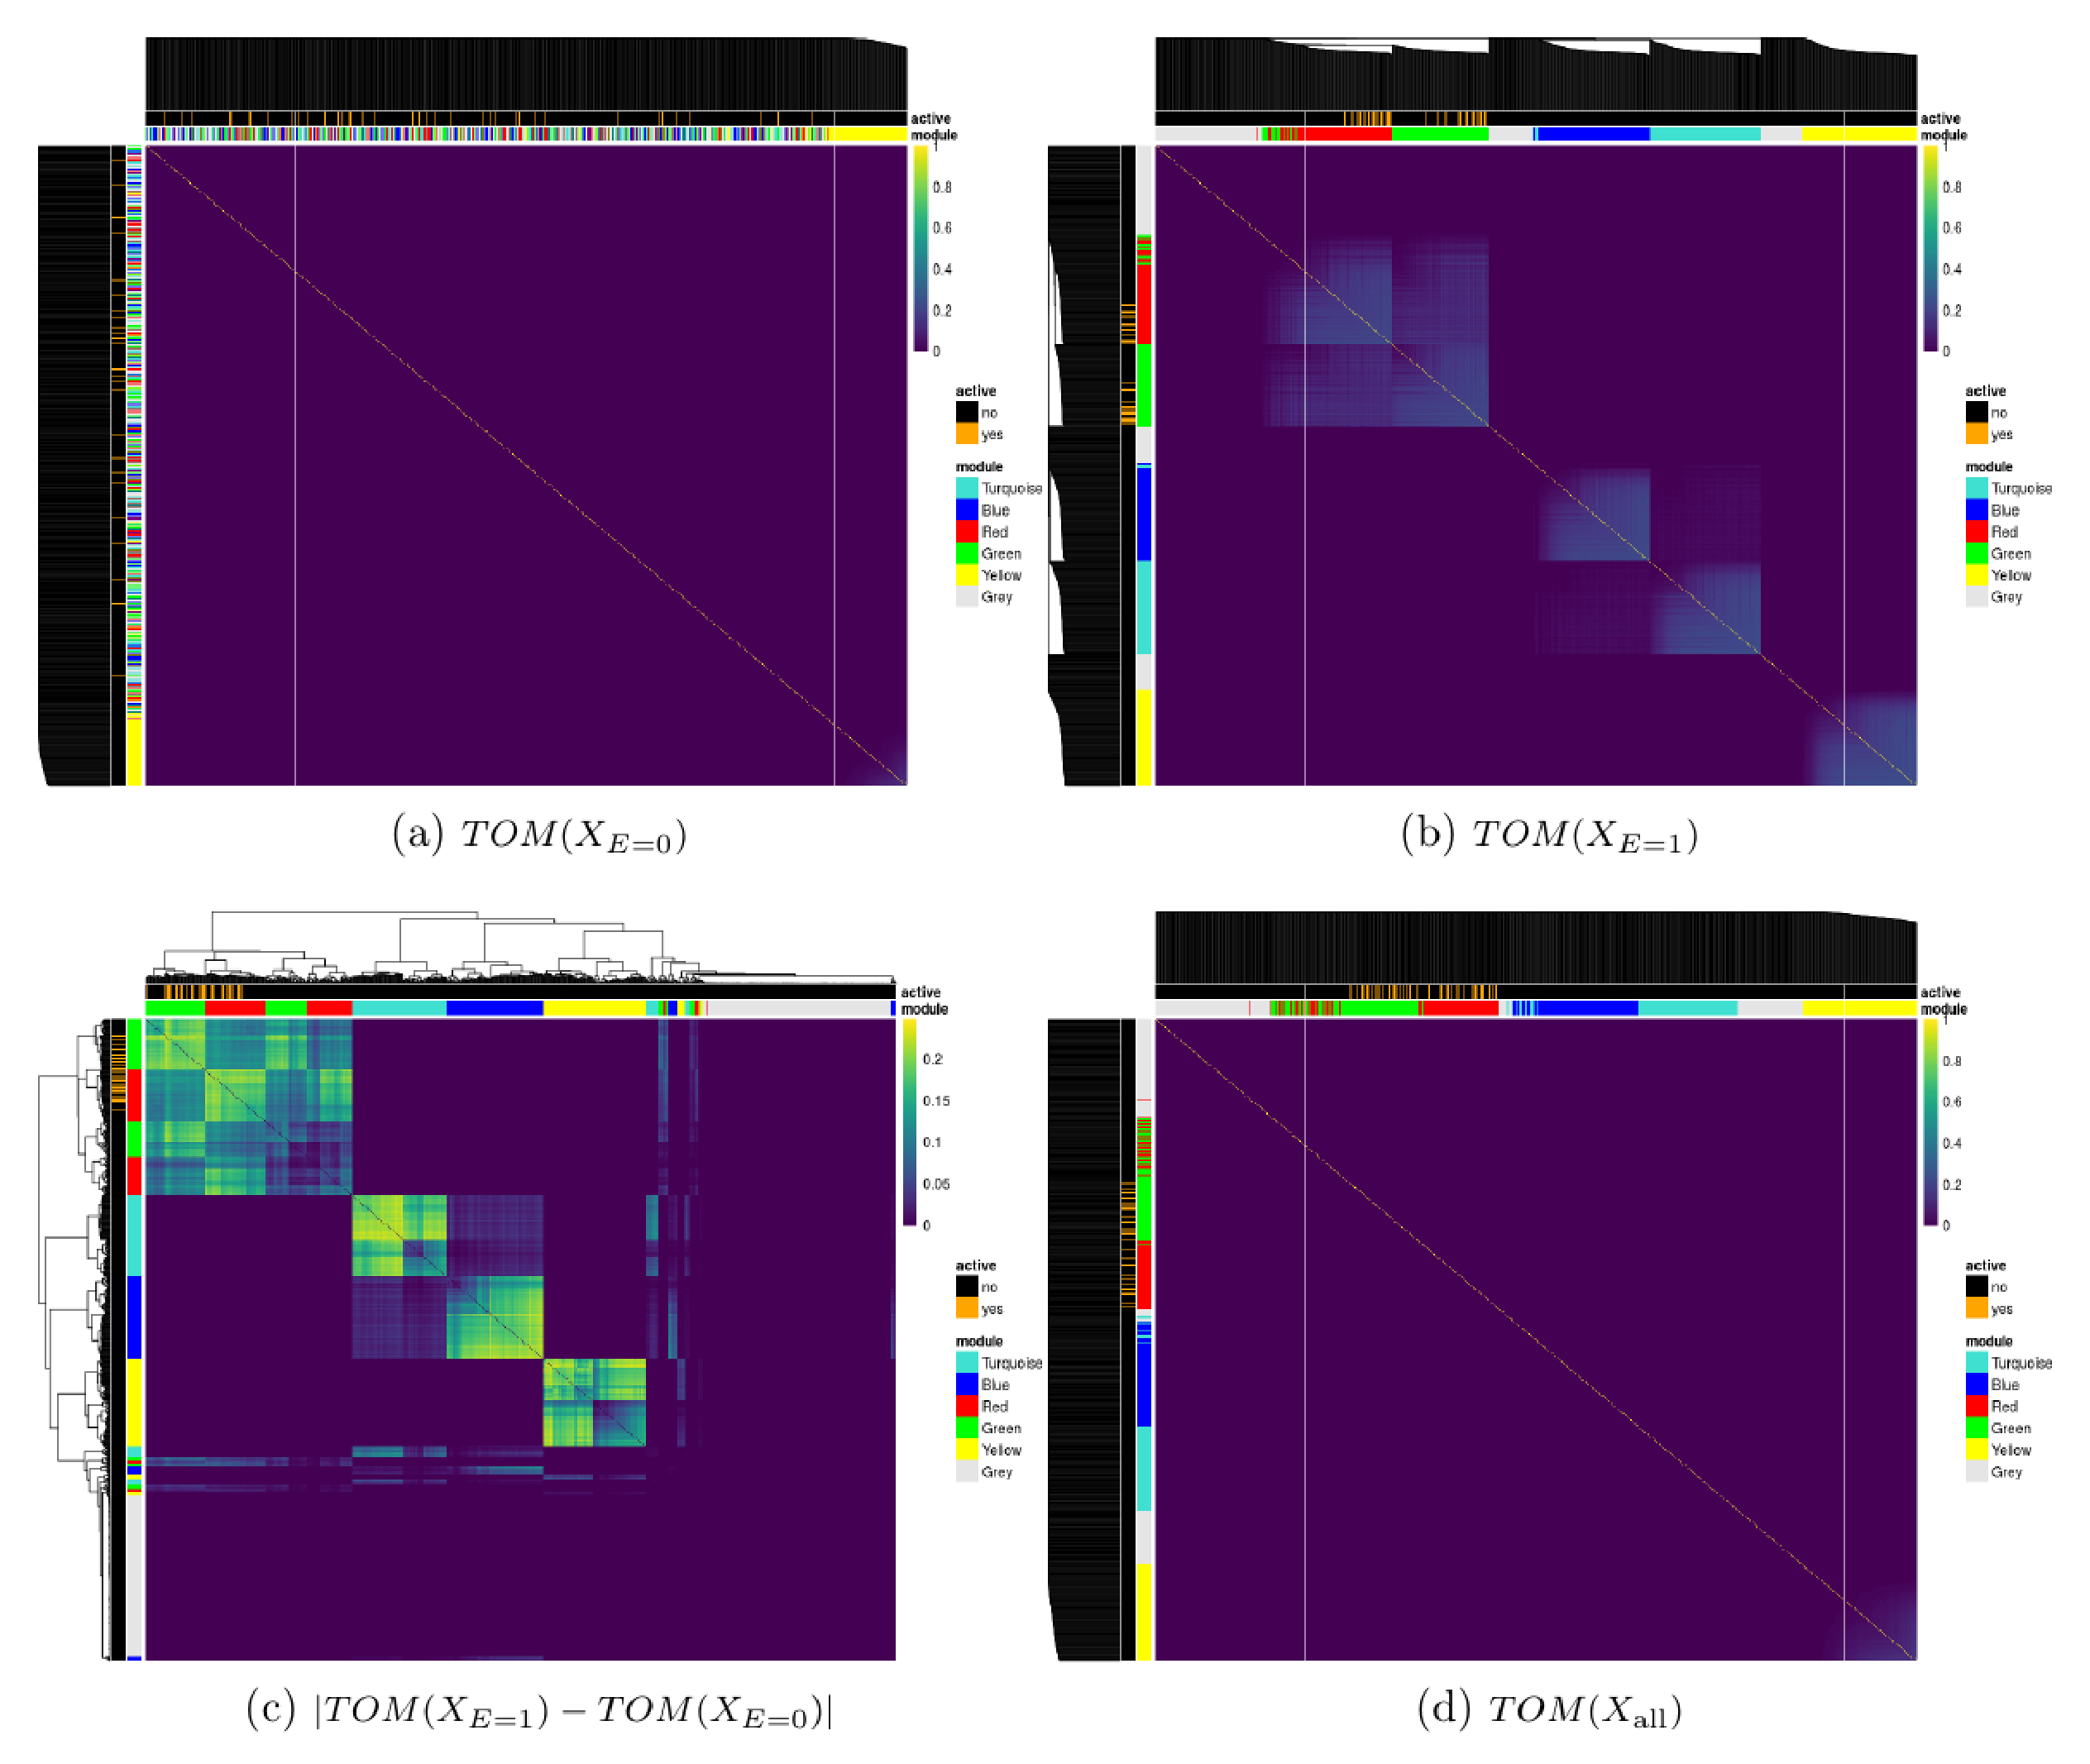
\includegraphics[scale=0.4, keepaspectratio]{figure3.eps}
	\caption{Topological overlap matrices (TOM) of simulated predictors based on subjects with (a) $E=0$, (b) $E=1$, (c) their absolute difference and (d) all subjects. Dendrograms are from hierarchical clustering (average linkage) of one minus the TOM for a, b, and d and the euclidean distance for c.   Some variables in the red and green clusters are associated with the outcome variable. The \textit{module} annotation represents the true cluster membership for each predictor, and the \textit{active} annotation represents the truly associated predictors with the response.}
	\label{fig:simTOM}
\end{figure}
\end{comment}

\fig{figure3}{simTOM}{16cm}{Topological overlap matrices (TOM) of simulated predictors based on subjects with (a) $E=0$, (b) $E=1$, (c) their absolute difference and (d) all subjects. Dendrograms are from hierarchical clustering (average linkage) of one minus the TOM for a, b, and d and the euclidean distance for c.   Some variables in the red and green clusters are associated with the outcome variable. The \textit{module} annotation represents the true cluster membership for each predictor, and the \textit{active} annotation represents the truly associated predictors with the response.}{Topological overlap matrices (TOM) of simulated predictors}



\subsection{The response}
The first three simulation scenarios differ in how the linear predictor $Y^*$ in~\eqref{eq:response} is defined, and also in the choice of regression model used to fit the data. In simulations 1 and 2 we use lasso~\citep{tibshirani1996regression} and elasticnet~\citep{zou2005regularization} to fit linear models; then we use MARS~\citep{friedman1991multivariate} in simulation 3 to estimate non-linear effects. Simulations 4, 5 and 6 use the GLM version of these models, respectively, since the responses are binary.

\subsection*{Simulation 1}
Simulation 1 was designed to evaluate performance when there are no explicit interactions between X and E (see Equation~\eqref{eq:2pred}). We generated the linear predictor from
\begin{equation}
Y^* = \sum_{\mathclap{\substack{j\in \left\lbrace 1, \ldots, 250 \right\rbrace\\ j \in \tm{ red, green block}}}}  \beta_j X_j + \beta_E E 
\end{equation}
where $\beta_j \sim \tm{Unif}\left[ 0.9,1.1\right]$ and \mbox{$\beta_E = 2$}. That is, only the first 250 predictors of both the red and green blocks are active. In this setting, only the main effects model is being fit to the simulated data. 


\subsection*{Simulation 2}
In the second scenario we explicitly simulated interactions. All non-zero main effects also had a corresponding non-zero interaction effect with $E$. We generated the linear predictor from
\begin{equation}
Y^* = \sum_{\mathclap{\substack{j\in \left\lbrace 1, \ldots, 125 \right\rbrace\\ j \in \tm{ red, green block}}}} \left(\beta_j X_j + \alpha_{j} X_j E\right) + \beta_E E 
\end{equation}
where $\beta_j \sim \tm{Unif}\left[ 0.9,1.1\right]$, $\alpha_{j} \sim \tm{Unif}\left[ 0.4,0.6\right]$ or $\alpha_{j} \sim \tm{Unif}\left[ 1.9,2.1\right]$, and \mbox{$\beta_E = 2$}. In this setting, both the main effects and their interactions with E are being fit to the simulated data. 

\subsection*{Simulation 3}
In the third simulation we investigated the performance of the ECLUST approach in the presence of non-linear effects of the predictors on the phenotype:
\begin{equation}
Y_i^* = \sum_{\mathclap{\substack{j\in \left\lbrace 1, \ldots, 250 \right\rbrace\\ j \in \tm{ red, green block}}}}  \beta_j X_{ij}  + \beta_E E_i + \alpha_Q E_i \cdot f(Q_i) \label{eq:sim3}
\end{equation} where 
\begin{align}
Q_i &= - \max_{\mathclap{\substack{\textcolor{white}{text} \\ j\in \left\lbrace 1, \ldots, 250 \right\rbrace\\ j \in \tm{ red, green block}}}}   \left(  X_{ij} - \bar{X}_i   \right)^2   \label{eq:qiterm}\\
f(u_i) &= \frac{u_i - \displaystyle \min_{i \in \left\lbrace 1, \ldots, n \right \rbrace  } u_i}{-\displaystyle \min_{i \in \left\lbrace 1, \ldots, n \right \rbrace  } u_i} \label{eq:fterm}\\
\bar{X}_i &= \frac{1}{500} \sum_{\mathclap{\substack{j\in \left\lbrace 1, \ldots, 250 \right\rbrace\\ j \in \tm{ red, green block}}}} X_{ij} \nonumber
\end{align}
The design of this simulation was partially motivated by considering the idea of canalization, where systems operate within appropriate parameters until sufficient perturbations accumulate (e.g.~\cite{gibson2009decanalization}). In this third simulation, we set $\beta_j \sim \tm{Unif}\left[ 0.9,1.1\right]$, \mbox{$\beta_E = 2$} and \mbox{$\alpha_Q = 1$}. We assume the data has been appropriately normalized, and that the correlation between any two features is greater than or equal to 0. In simulation 3, we tried to capture the idea that an exposure could lead to coregulation or disregulation of a cluster of $X$'s, which in itself directly impacts Y.  Hence, we defined coregulation as the $X$'s being similar in magnitude and disregulation as the $X$'s being very different. The $Q_i$ term in~\eqref{eq:qiterm} is defined such that higher values would correspond to strong coregulation whereas lower values correspond to disregulation. For example, suppose $Q_i$ ranges from -5 to 0. It will be -5 when there is lots of variability (disregulation) and 0 when there is none (strong coregulation). The function $f(\cdot)$ in~\eqref{eq:fterm} simply maps $Q_i$ to the [0,1] range. In order to get an idea of the relationship in~\eqref{eq:sim3}, Figure~\ref{fig:sim3-perp} displays the response $Y$ as a function of the first principal component of $\sum_j \beta_j X_{ij}$ (denoted by \texttt{1st PC}) and $f(Q_i)$.   We see that lower values of $f(Q_i)$ (which implies disregulation of the features) leads to a lower $Y$. In this setting, although the clusters do not explicitly include interactions between the $X$ variables,  the MARS algorithm allows for the possibility of two way interactions between any of the variables. 
\begin{comment}
\begin{figure}[h!]
	\centering
	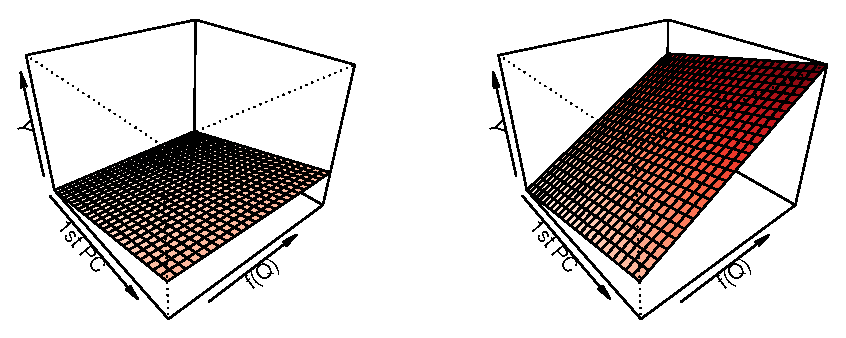
\includegraphics[scale=1, keepaspectratio]{figure4.eps}
	\caption{Visualization of the relationship between the response, the first principal component of the main effects and $f(Q_i)$ in~\eqref{eq:sim3} for $E=0$ (left) and $E=1$ (right) in simulation scenario 3. This graphic also depicts the intuition behind model~\eqref{eq:nonlinear}.}
	\label{fig:sim3-perp}
\end{figure}
\end{comment}


\fig{figure4}{sim3-perp}{16cm}{Visualization of the relationship between the response, the first principal component of the main effects and $f(Q_i)$ in~\eqref{eq:sim3} for $E=0$ (left) and $E=1$ (right) in simulation scenario 3. This graphic also depicts the intuition behind model~\eqref{eq:nonlinear}.}{Visualization of the relationship between the response, the first principal component of the main effects and $f(Q_i)$ in simulation scenario 3.}

\subsection*{Simulations 4, 5 and 6}
We used the same simulation setup as above, except that we took the continuous outcome $Y$, defined $p = 1/(1+exp(-Y))$ and used this to generate a two-class outcome $z$ with $\tm{Pr}(z=1)=p$ and $\tm{Pr}(z=0)=1-p$. The true parameters were simulated as $\beta_j \sim \tm{Unif}[\log(0.9), \log(1.1)]$, $\beta_E = \log(2)$, $\alpha_j \sim \tm{Unif}[\log(0.4), \log(0.6)]$ or $\alpha_j \sim \tm{Unif}[\log(1.9), \log(2.1)]$. Simulations 4, 5 and 6 are the binary response versions of simulations 1, 2 and 3, respectively. The larger odds ratio for E compared to the odds ratio for X is motivated by certain environmental factors which are well known to have substantial impacts on disease risks and phenotypes. For example, body mass index has been estimated to explain a large proportion of variation in bone mineral density (BMD) in women (10-20\%)~\citep{felson1993effects}. This can be converted to a slope of 0.31-0.44 assuming variables are standardized, i.e., changes of 0.3-0.4 standard deviations in BMD per standard deviation change in weight. In contrast, the majority of SNPs and rare variants have effect sizes under 0.10 standard deviations on BMD~\citep{kemp2017identification}.

\subsection{Measures of Performance}
Simulation performance was assessed with measures of model fit, prediction accuracy and feature stability. Several measures for each of these categories, and the specific formulae used are provided in Table~\ref{tab:measures}. We simulated both a training data set and a test data set for each simulation: all tuning parameters for  model selection were selected using the training sets only.  Although most of the measures of model fit were calculated on the test data sets, true positive rate, false positive rate and correct sparsity were calculated on the training set only. The root mean squared error is determined by predicting the response for the test set using the fitted model on the training set. The area under the curve is determined using the trapezoidal rule~\citep{auc}. The stability of feature importance is defined as the variability of feature weights under perturbations of the training set, i.e., small modifications in the training set should not lead to considerable changes in the set of important covariates~\citep{tolocsi2011classification}. A feature selection algorithm produces a weight (e.g. $\boldsymbol{\beta}= (\beta_1, \ldots, \beta_p)$), a ranking (e.g. $rank(\boldsymbol{\beta}):\mb{r} = (r_1, \ldots, r_m)$) and a subset of features (e.g. $\mb{s}=(s_1,\ldots, s_p), s_j = \mathbb{I}\left\lbrace\beta_j\neq 0 \right\rbrace$ where $\mathbb{I}\left\lbrace \cdot\right\rbrace$ is the indicator function). 
In the CLUST and ECLUST methods, we defined a predictor to be non-zero if its corresponding cluster representative weight was non-zero. Using 10-fold cross validation (CV), we evaluated the similarity between two features and their rankings using Pearson and Spearman correlation, respectively. For each CV fold we re-ran the models and took the average Pearson/Spearman correlations of the $\binom{10}{2}$ combinations of estimated coefficients vectors. To measure the similarity between two subsets of features we took the average of the Jaccard distance in each fold. A Jaccard distance of 1 indicates perfect agreement between two sets while no agreement will result in a distance of 0. For MARS models we do not report the Pearson/Spearman stability rankings due to the adaptive and functional nature of the model (there are many possible combinations of predictors, each of which are linear basis functions). 
\begin{table}[h]	
	\begin{threeparttable}
		\caption{Measures of Performance}
		\label{tab:measures}
		\begin{tabulary}{\linewidth}{lc}
			\toprule
Measure                   & Formula	 \\ \midrule
\textit{\underline{Model Fit}} \\
\,\,\,\, True Positive Rate (TPR) & $\sfrac{|\widehat{S} \in  S_0|}{|S_0|}$ \\ 
\addlinespace[5pt] 
\,\,\,\, False Positive Rate (TPR) & $\sfrac{|\widehat{S} \notin S_0|}{|j \notin S_0|} $ \\ 
\addlinespace[5pt] \\
\,\,\,\, Correct Sparsity~\citep{witten2014cluster} & $\frac{1}{p} \sum_{j=1}^{p} A_j $ \\
\addlinespace[4pt]
& $A_j = \begin{cases}
1 & \tm{if } \hat{\beta_j}= \beta_j = 0\\
1 & \tm{if } \hat{\beta_j}\neq 0, \beta_j \neq 0\\
0 & \tm{if } \tm{else}
\end{cases}$\\
\addlinespace[5pt] 
\textit{\underline{Prediction Accuracy}} \\
\,\,\,\, Root Mean Squared Error (RMSE) & $\norm{\mb{Y}_{test}- \widehat{\bs{\mu}}(\mb{X}_{test})}_2$ \\
%\addlinespace[10pt] \\
\,\,\,\, Area Under the Curve (AUC) & Trapezoidal rule \\
\,\,\,\, Hosmer-Lemeshow Test ($G=10$) & $\chi^2$ test statistic \\
\addlinespace[5pt] \\
\multicolumn{2}{l}{\textit{\underline{Feature Stability using $K$-fold Cross-Validation on training set~\citep{kalousis2007stability}}}} \\
\addlinespace[4pt]
\,\,\,\, Pearson Correlation $(\rho)$~\citep{pearson1895note} & $ \binom{K}{2}^{-1}\sum\limits_{i,j \in \left\lbrace 1, \ldots, K \right\rbrace, i \neq j} \frac{cov\left(\widehat{\mb{\beta}}_{(i)},\widehat{\mb{\beta}}_{(j)}\right)}{\sigma_{\widehat{\mb{\beta}}_{(i)}} \sigma_{\widehat{\mb{\beta}}_{(j)}} }$ \\ 
\addlinespace[10pt]
\,\,\,\, Spearman Correlation ($r$)~\citep{spearman1904proof} & $\binom{K}{2}^{-1}\sum\limits_{i,j \in \left\lbrace 1, \ldots, K \right\rbrace, i \neq j} \left[ 1 - 6 \sum\limits_{m} \frac{\left( r_{m_{(i)}} - r_{m_{(j)}}\right) ^2}{p(p^2-1)}\right] $\\
\addlinespace[10pt] 
\,\,\,\, Jaccard Distance~\citep{jaccard1912distribution} & $\frac{|\widehat{S}_{(i)} \cap \widehat{S}_{(j)} |}{ |\widehat{S}_{(i)} \cup \widehat{S}_{(j)} |}$  \\ \bottomrule
		\end{tabulary}
		\begin{tablenotes}[para,flushleft]
			{\footnotesize
				%\textit{Note.} sfs
			\tabfnt{a}$\widehat{\bs{\mu}}$: fitting procedure on the training set
			\tabfnt{b}$S_0$: index of active set $ = \left\lbrace j; \beta_j^0 \neq 0 \right\rbrace$
			\tabfnt{c}$\widehat{S}$: index of the set of non-zero estimated coefficients $ = \left\lbrace j; \widehat{\beta}_j \neq 0 \right\rbrace$
		    \tabfnt{d}$|A|$: is the cardinality of set $A$				
			}
		\end{tablenotes} 		
	\end{threeparttable}
\end{table}	

\subsection{Results}
All reported results are based on 200 simulation runs. We graphically summarized the results across simulations 1-3 for model fit (Figure~\ref{fig:sim-modelfit}) and feature stability (Figure~\ref{fig:sim-stability}). The results for simulations 4-6 are shown in the Supplemental Section B, Figures S1-S6. We restrict our attention to $SNR=1$, $\rho = 0.9$, and $\alpha_{j} \sim \tm{Unif}\left[1.9, 2.1\right]$. The model names are labeled as \texttt{summary measure\_model} (e.g. \texttt{avg\_lasso} corresponds using the average of the features in a cluster as inputs into a lasso regression model). When there is no summary measure appearing in the model name, that indicates that the original variables were used (e.g. \texttt{enet} means all separate features were used in the elasticnet model). In panel A of Figure~\ref{fig:sim-modelfit}, we plot the true positive rate against the false positive rate for each of the 200 simulations. We see that across all simulation scenarios, the SEPARATE method has extremely poor sensitivity compared to both CLUST and ECLUST, which do much better at identifying the active variables, though the resulting models are not always sparse. The relatively few number of green points in panel A is due to the small number of estimated clusters (Supplemental Section C, Figure S7) leading to very little variability in performance across simulations. The better performance of ECLUST over CLUST is noticeable as more points lie in the top left part of the plot. The horizontal banding in panel A reflects the stability of the TOM-based clustering approach.
%The discrete nature of the plots demonstrates the stability of the clustering algorithm. 
ECLUST also does better than CLUST in correctly determining whether a feature is zero or nonzero (Figure~\ref{fig:sim-modelfit}, panel B). Importantly, across all three simulation scenarios, ECLUST outperforms the competing methods in terms of RMSE (Figure~\ref{fig:sim-modelfit}, panel C), regardless of the summary measure and modeling procedure. We present the distribution for the effective number of variables selected in the supplemental material (Figures S8 and S9). We see that the median number of variables selected from ECLUST is less than the median number of variables selected from CLUST, though ECLUST has more variability.

\begin{comment}
\begin{figure}[H]
	\centering
	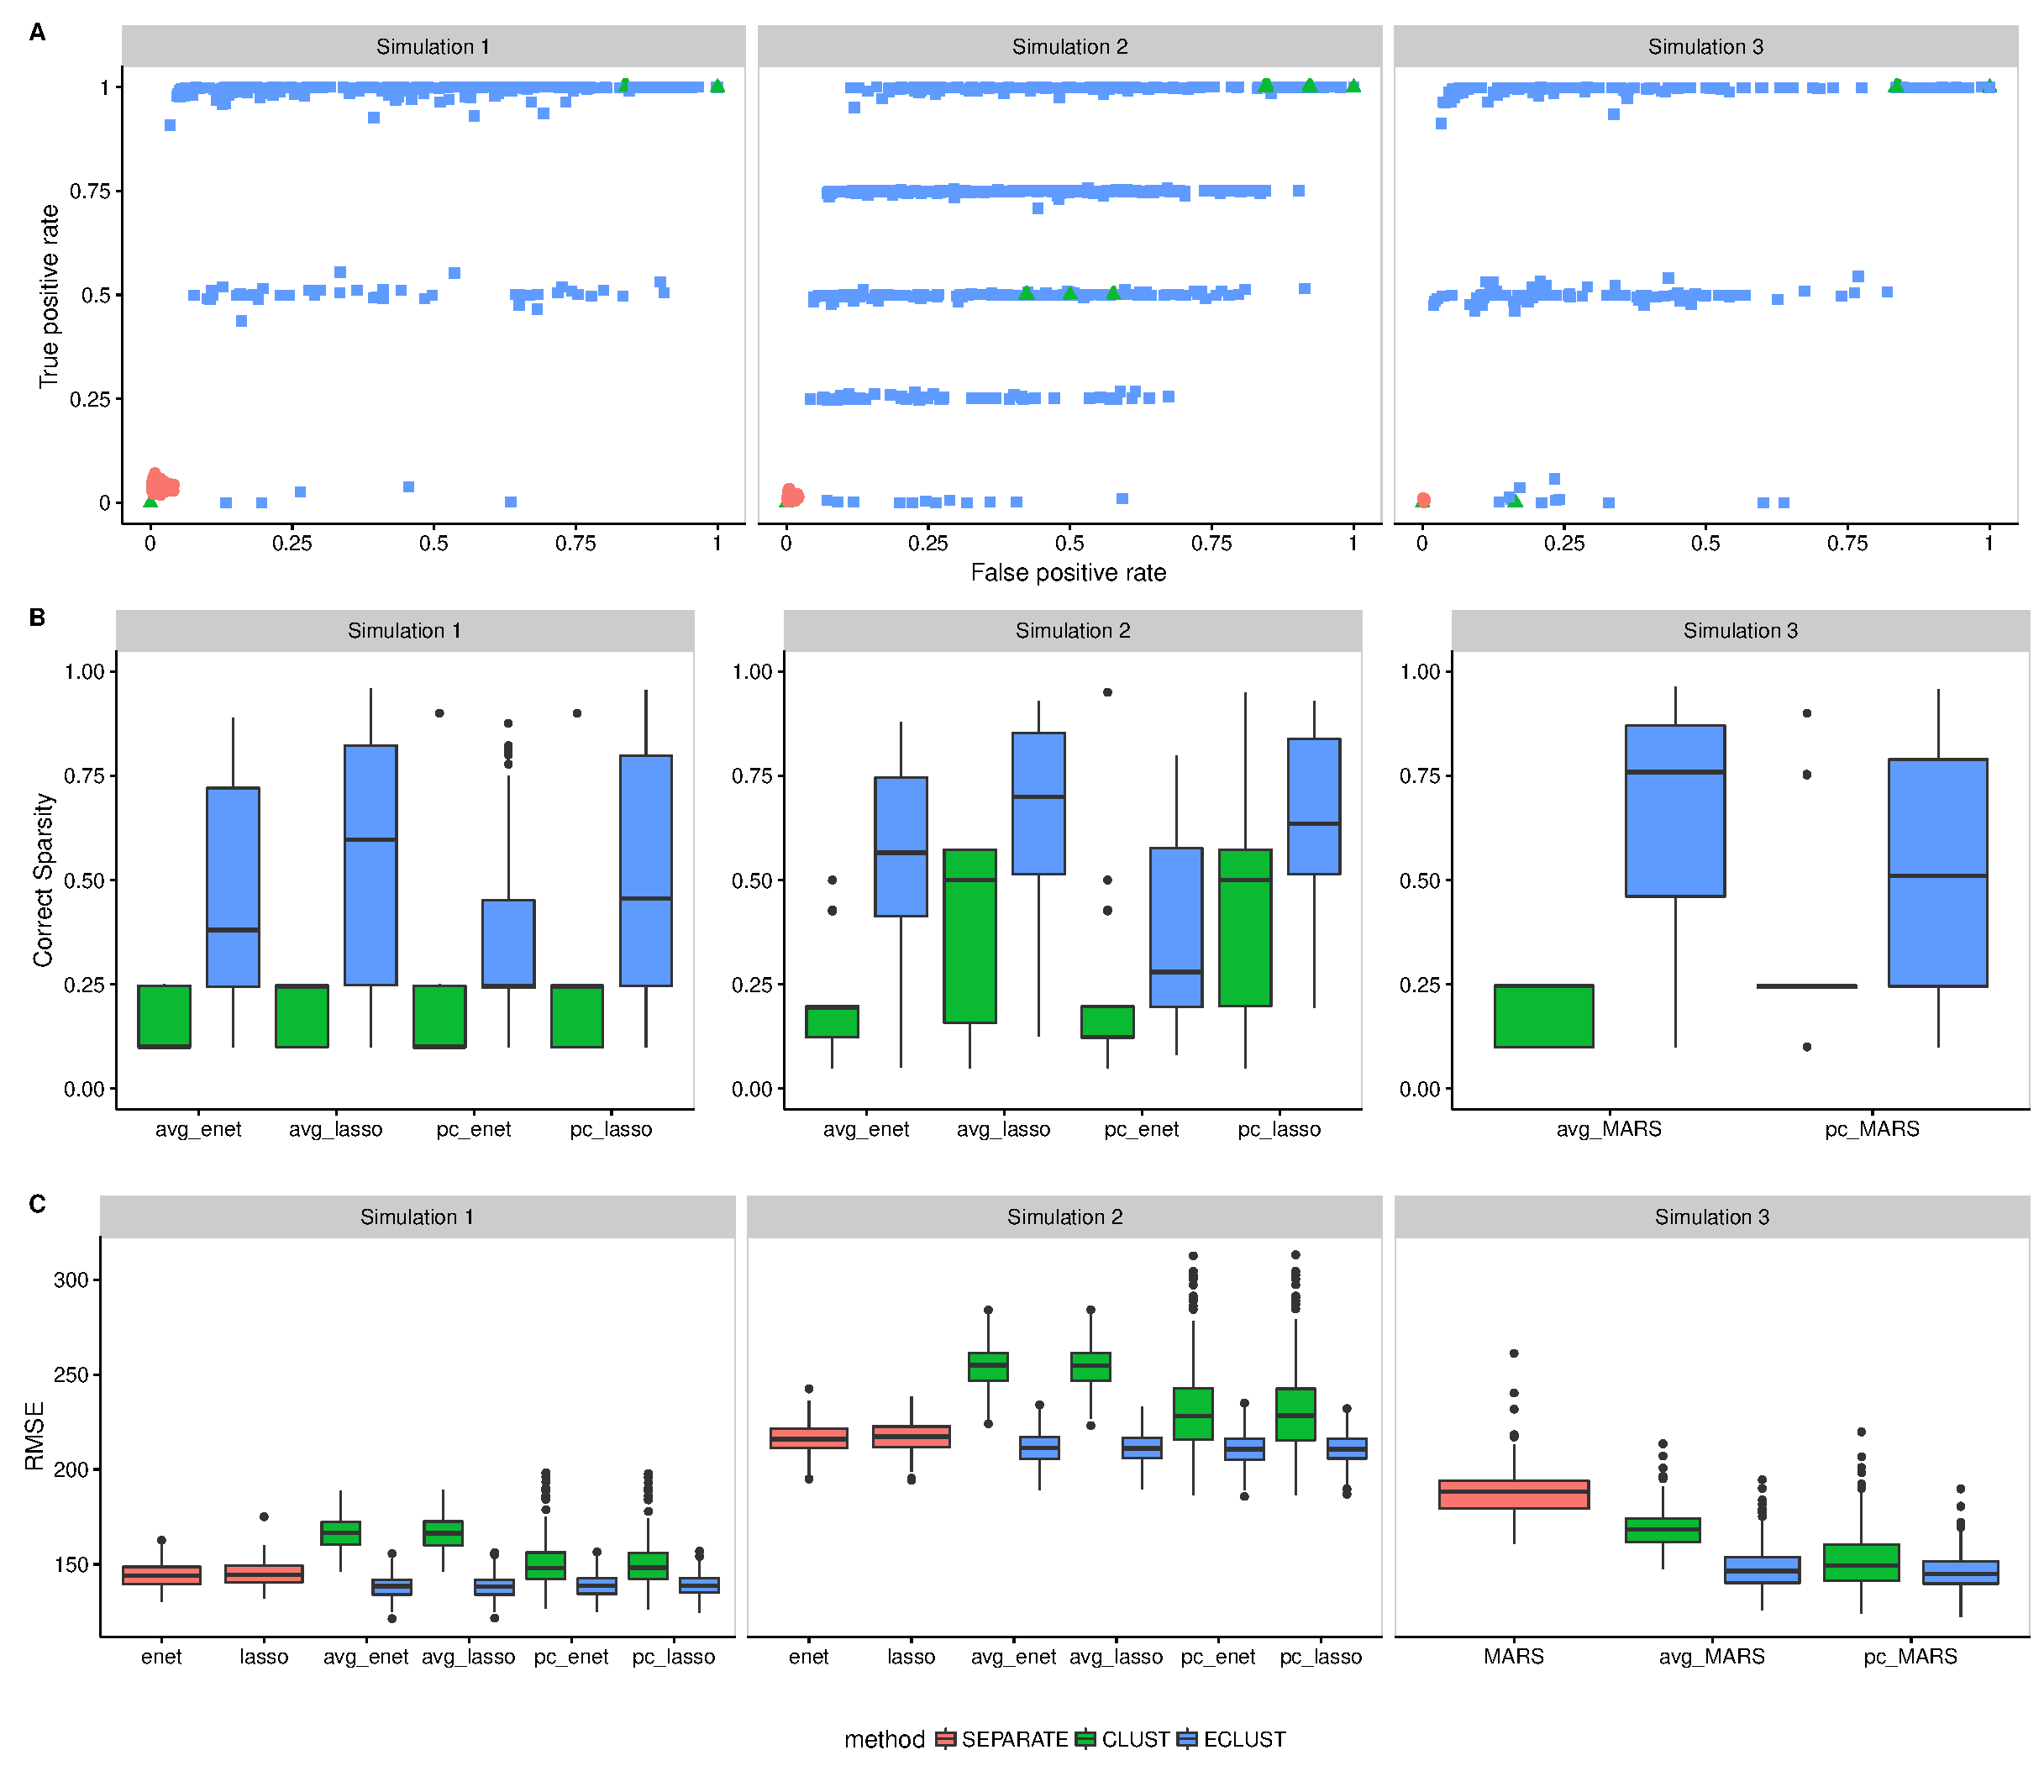
\includegraphics[scale=0.40, keepaspectratio]{figure5.eps}
	\caption{Model fit results from simulations 1, 2 and 3 with $SNR=1$, $\rho = 0.9$, and $\alpha_{j} \sim \tm{Unif}\left[1.9, 2.1\right]$. SEPARATE results are in pink, CLUST in green and ECLUST in blue.}
	\label{fig:sim-modelfit}
\end{figure}
\end{comment}


\fig{figure5}{sim-modelfit}{16cm}{Model fit results from simulations 1, 2 and 3 with $SNR=1$, $\rho = 0.9$, and $\alpha_{j} \sim \tm{Unif}\left[1.9, 2.1\right]$. SEPARATE results are in pink, CLUST in green and ECLUST in blue.}{Model fit results from simulations 1, 2 and 3.}


While the approach using all separate original variables (SEPARATE) produce sparse models, they are sensitive to small perturbations of the data across all stability measures (Figure~\ref{fig:sim-stability}), i.e, similar datasets produce very different models. 
Although the median for the CLUST approach is always slightly better than the median for ECLUST across all stability measures, CLUST results can be much more variable, particularly when stability is measured by the agreement between the value and the ranking of the estimated coefficients across CV folds (Figure~\ref{fig:sim-stability}, panels B and C). The number of estimated clusters, and therefore the number of features in the regression model, tends to be much smaller in CLUST compared to ECLUST, and this explains its poorer performance using the stability measures in Figure~\ref{fig:sim-stability}, since there are more coefficients to estimate. Overall, we observe that the relative performance of ECLUST versus CLUST in terms of stability is consistent across the two summary measures (average or principal component) and across the penalization procedures. The complete results for different values of $\rho$, $SNR$ and $\alpha_{j}$ (when applicable) are available in the Supplemental Section D, Figures S10-S15 for Simulation 1, Figures S16 - S21 for Simulation 2, and Figures S22 - S25 for Simulation 3. They show that these conclusions are not sensitive to the $SNR$, $\rho$ or $\alpha_j$. Similar conclusions are made for a binary outcome using logistic regression versions of the lasso, elasticnet and MARS. ECLUST and CLUST also have better calibration than the SEPARATE method for both linear and non-linear models (Supplemental Section B, Figures S3-S6). The distributions of Hosmer-Lemeshow (HL) $p$-values do not follow uniformity. This is in part due to the fact that the HL test has low power in the presence of continuous-dichotomous variable interactions~\citep{hosmer1997comparison}. Upon inspection of the Q-Q plots, we see that the models have difficulty predicting risks at the boundaries which is a known issue in most models. We also have a small sample size of 200, which means there are on average only 20 subjects in each of the 10 bins. Furthermore, the HL test is sensitive to the choice of bins and method of computing quantiles. Nevertheless, the improved fit relative to the SEPARATE analysis is quite clear.

We also ran all our simulations using the Pearson correlation matrix as a measure of similarity in order to compare its performance against the TOM. The complete results are in the Supplemental Section E, Figures S26-S31 for Simulation 1, Figures S32 - S37 for Simulation 2, and Figures S38 - S41 for Simulation 3. In general, we see slightly better performance of CLUST over ECLUST when using Pearson correlations.  This result is probably due to the imprecision in the estimated correlations.  The exposure dependent similarity matrices are quite noisy, and the variability is even larger when we examine the differences between two correlation matrices.  Such large levels of variability have a negative impact on the clustering algorithm's ability to detecting the true clusters.

\begin{comment}
\begin{figure}[h!]
	\centering
	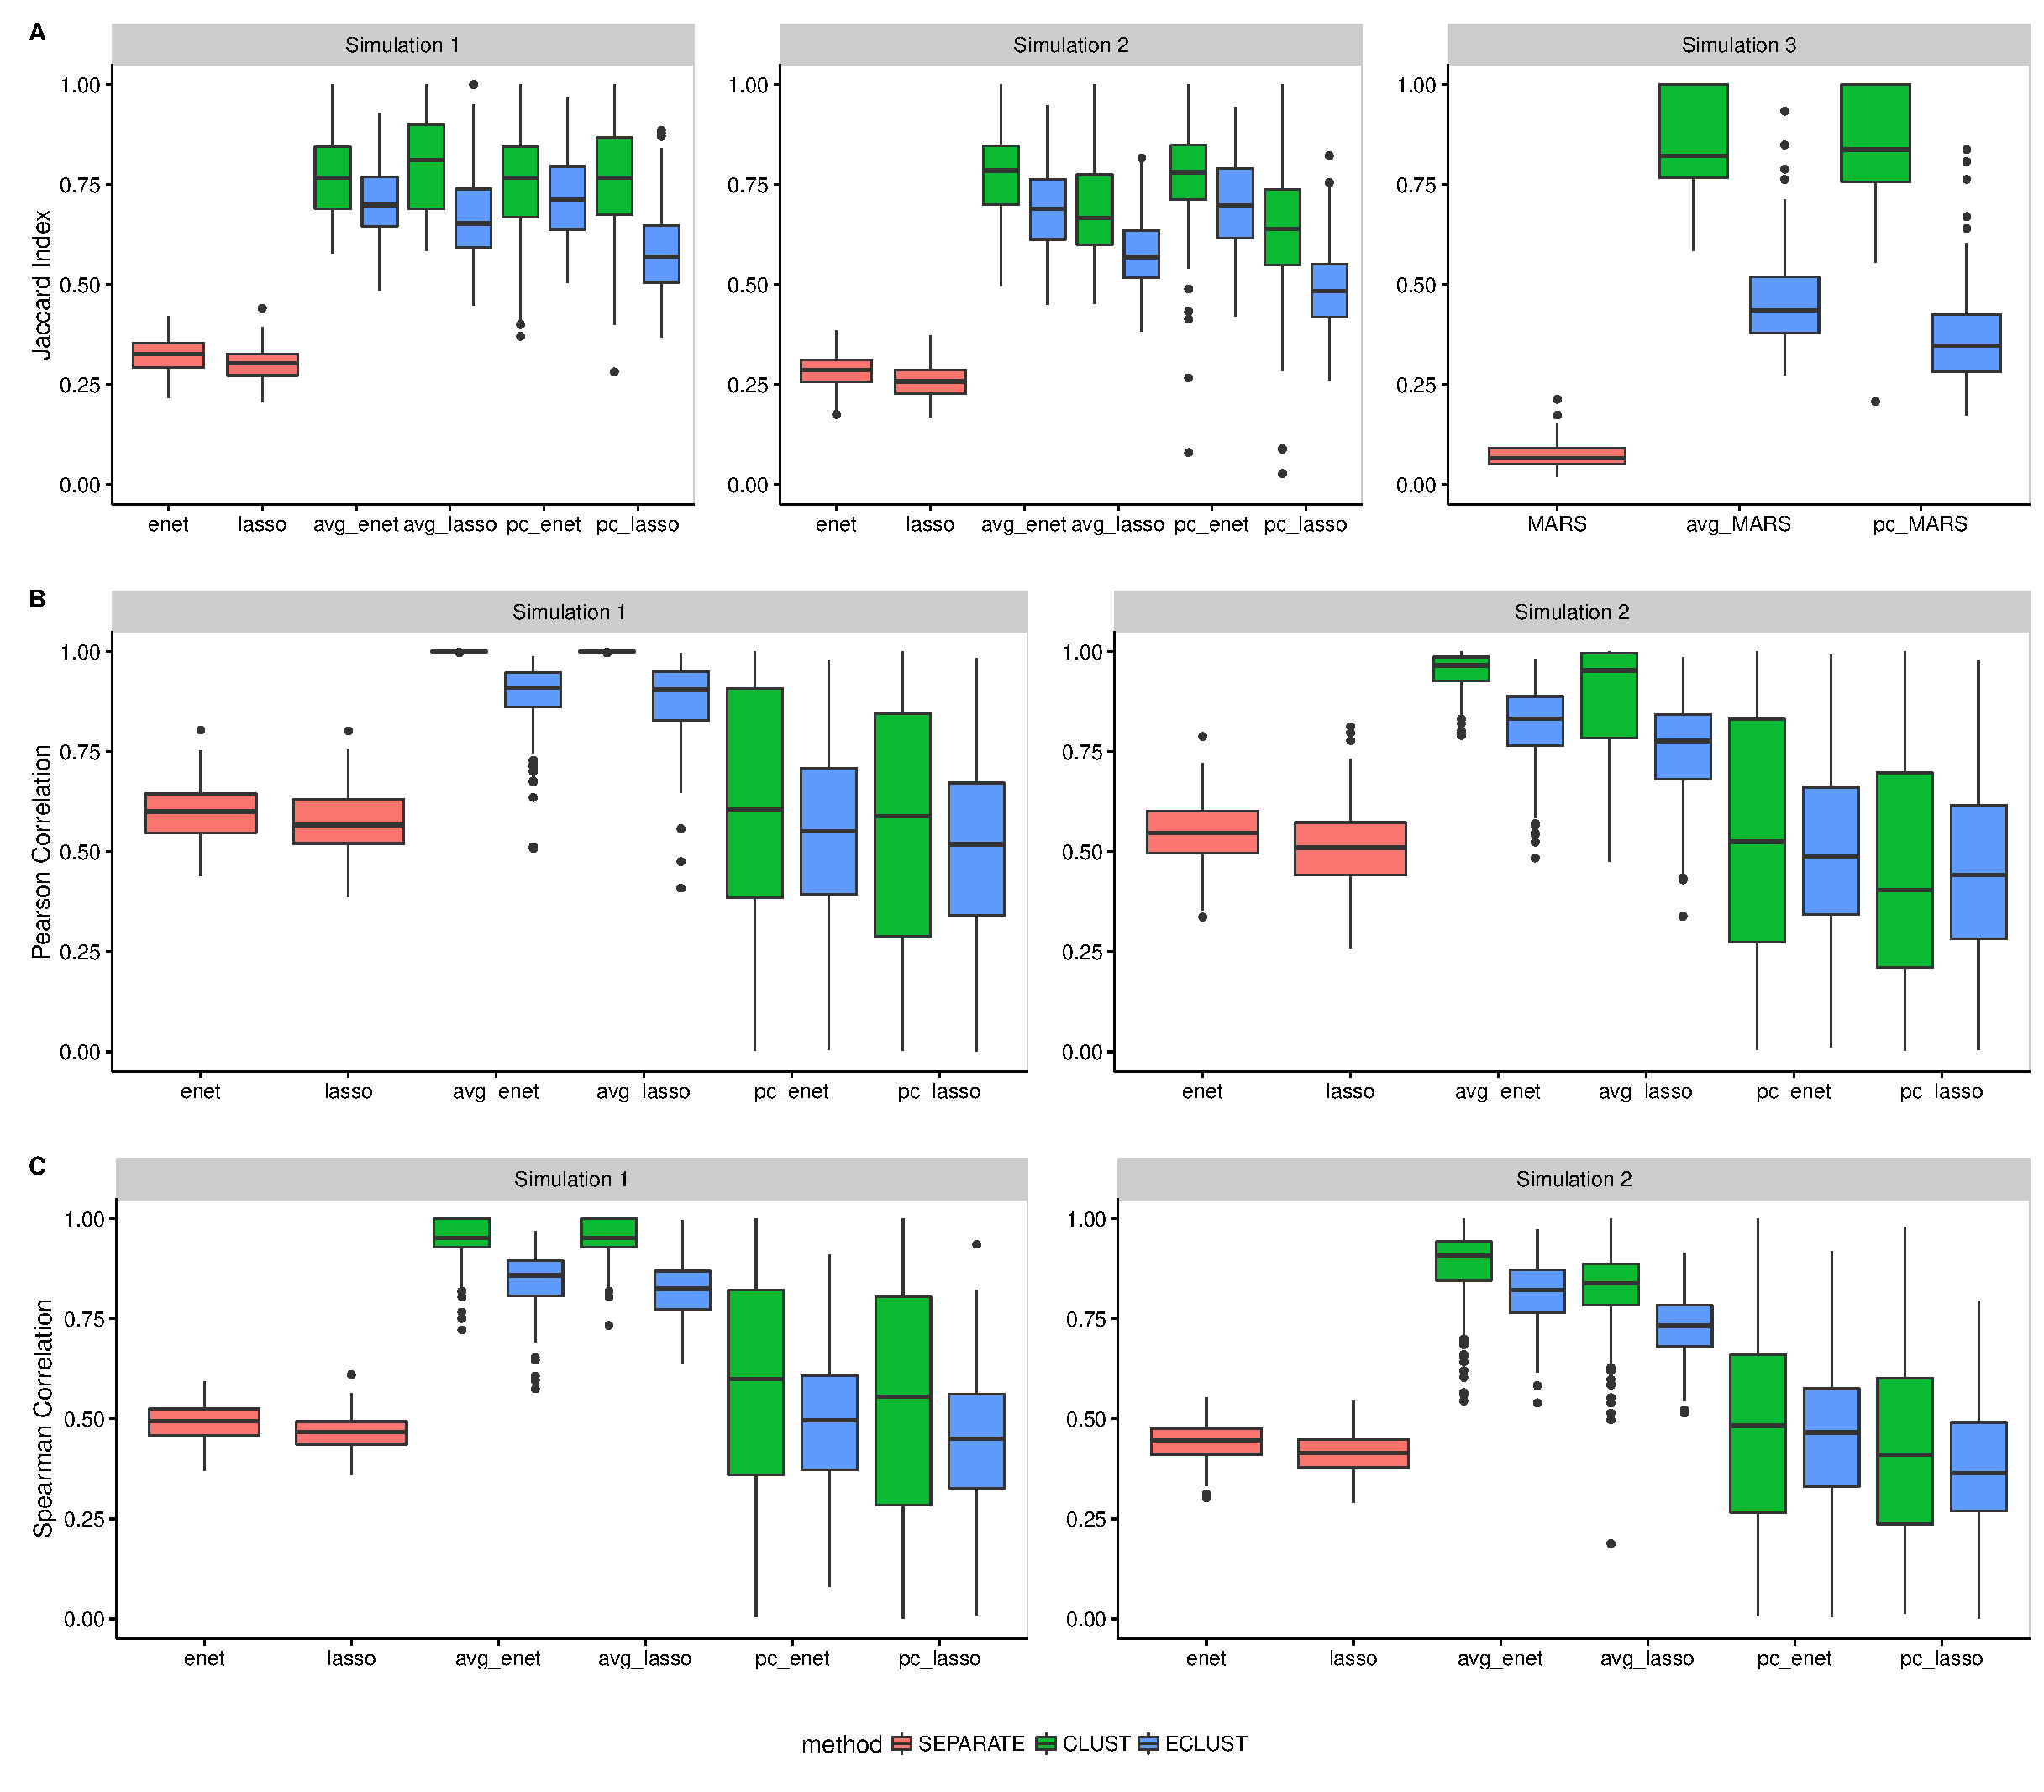
\includegraphics[scale=0.40, keepaspectratio]{figure6.eps}
	\caption{Stability results from simulations 1, 2 and 3 for $SNR=1$, $\rho = 0.9$, and $\alpha_{j} \sim \tm{Unif}\left[1.9, 2.1\right]$. SEPARATE results are in pink, CLUST in green and ECLUST in blue.}
	\label{fig:sim-stability}
\end{figure}
\end{comment}


\fig{figure6}{sim-stability}{16cm}{Stability results from simulations 1, 2 and 3 for $SNR=1$, $\rho = 0.9$, and $\alpha_{j} \sim \tm{Unif}\left[1.9, 2.1\right]$. SEPARATE results are in pink, CLUST in green and ECLUST in blue.}{Stability results from simulations 1, 2 and 3.}

\section{Analysis of three data sets}

In this section we demonstrate the performance of ECLUST on three high dimensional datasets with contrasting motivations and features. In the first data set, normal brain development is examined in conjunction with intelligence scores. In the second data set we aim to identify molecular subtypes of ovarian cancer using gene expression data. The investigators' goal in the third data set is to examine the impact of gestational diabetes mellitus (GDM) on childhood obesity in a sample of mother-child pairs from a prospective birth cohort. The datasets comprise a range of sample sizes, and both the amount of clustering in the HD data and the strength of the effects of the designated exposure variables vary substantially.  Due to the complex nature of these datasets, we decided to use MARS models for step 2 of our algorithm for all 3 datasets, as outlined in Table~\ref{tab:eclust}. In order to assess performance in these data sets, we have computed the 0.632 estimator~\citep{efron1983estimating} and the 95\% confidence interval of the $R^2$ and RMSE from 100 bootstrap samples. The $R^2$ reported here is defined as the squared Pearson correlation coefficient between the observed and predicted response~\citep{kvaalseth1985cautionary}, and the RMSE is defined as in Table~\ref{tab:measures}. Because MARS models can result in unstable predictors~\citep{kuhn2008caret}, we also report the results of bagged MARS from $B=50$ bootstrap samples, where bagging~\citep{breiman1996bagging} refers to averaging the predictions from each of the MARS models fit on the $B$ bootstrap samples. 
%Results are summarized in Figure~\ref{fig:rda}.


\subsection{NIH MRI Study of Normal Brain Development} \label{sec:nih}

The NIH MRI Study of Normal Brain Development, started in 2001, was a 7 year longitudinal multi-site project that used magnetic resonance technologies to characterize brain maturation in 433 medically healthy, psychiatrically normal children aged 4.5-18 years~\citep{evans2006nih}. The goal of this study was to provide researchers with a representative and reliable source of healthy control subject data as a basis for understanding atypical brain development associated with a variety of developmental, neurological, and neuropsychiatric disorders affecting children and adults. Brain imaging data (e.g. cortical surface thickness, intra-cranial volume), behavioural measures (e.g. IQ scores, psychiatric interviews, behavioral ratings) and demographics (e.g. socioeconomic status) were collected at two year intervals for three time points and are publicly available upon request. Previous research using these data found that level of intelligence and age correlate with cortical thickness~\citep{shaw2006intellectual, khundrakpam2013developmental}, but to our knowledge no such relation between income and cortical thickness has been observed. We therefore used this data to see the performance of ECLUST in the presence (age) and absence (income) of an effect on the correlations in the HD data. We analyzed the 10,000 most variable regions on the cortical surface from brain scans corresponding to the first sampled time point only. We used binary age (166 age~$\leq 11.3$ and 172~$>11.3$) and binary income (142 high and 133 low income) indicator as the environment variables and standardized IQ scores as the response. We identified 22 clusters from $TOM(X_{\tm{all}})$ and 57 clusters from $TOM(X_{\tm{diff}})$ when using age as the environment, and 86 clusters from $TOM(X_{\tm{all}})$ and 49 clusters from $TOM(X_{\tm{diff}})$ when using income as the environment. Results are shown in Figure~\ref{fig:rda}, panels C and D. The method which uses all individual variables as predictors (pink), has better $R^2$ but also worse RMSE compared to CLUST and ECLUST, likely due to over-fitting. There is a slight benefit in performance for ECLUST over CLUST when using age as the environment (panel D). Importantly, we observe very similar performance between CLUST and ECLUST across all models (panel C), suggesting very little impact on the prediction performance when including features derived both with and without the $E$ variable, in a situation where they are unlikely to be relevant. 


\subsection{Gene Expression Study of Ovarian Cancer}

Differences in gene expression profiles have led to the identification of robust molecular subtypes of ovarian cancer; these are of biological and clinical importance because they have been shown to correlate with overall survival~\citep{tothill2008novel}. Improving prediction of survival time based on gene expression signatures can lead to targeted therapeutic interventions~\citep{helland2011deregulation}. The proposed ECLUST algorithm was applied to gene expression data from 511 ovarian cancer patients profiled by the Affymetrix Human Genome U133A 2.0 Array. The data were obtained from the TCGA Research Network: http://cancergenome.nih.gov/ and downloaded via the TCGA2STAT R library~\citep{tcga2stat}. Using the 881 signature genes from~\cite{helland2011deregulation} we grouped subjects into two groups based on the results in this paper, to create a ``positive control'' environmental variable expected to have a strong effect. Specifically, we defined an environment variable in our framework as: $E=0$ for subtypes C1 and C2 ($n = 253$), and $E=1$ for subtypes C4 and C5 ($n = 258$). Overall survival time (log transformed) was used as the response variable. Since these genes were ascertained on survival time, we expected the method using all genes without clustering to have the best performance, and hence one goal of this analysis was to see if ECLUST performed significantly worse as a result of summarizing the data into a lower dimension. We found 3 clusters from $TOM(X_{\tm{all}})$ and 3 clusters from $TOM(X_{\tm{diff}})$;  results are shown in Figure~\ref{fig:rda}, panel C. Across all models, ECLUST performs slightly better than CLUST. Furthermore it performs almost as well as the separate variable method, with the added advantage of dealing with a much smaller number of predictors (881 with SEPARATE compared to 6 with ECLUST).  

\subsection{Gestational diabetes, epigenetics and metabolic disease}
Events during pregnancy are suspected to play a role in childhood obesity development but only little is known about the mechanisms involved. Indeed, children born to women who had GDM in pregnancy are more likely to be overweight and obese~\citep{wendland2012gestational}, and evidence suggests epigenetic factors are important piece of the puzzle~\citep{bouchard2010leptin,bouchard2012placental}. Recently, methylation changes in placenta and cord blood were associated with GDM~\citep{ruchat2013gestational}, and here we explore how these changes are associated with obesity in the children at the age of about 5 years old.   DNA methylation in placenta was measured with the Infinium HumanMethylation450 BeadChip (Illumina, Inc~\citep{bibikova2011high}) microarray, in a sample of 28 women, 20 of whom had a GDM-affected pregnancy, and here, we used GDM status as our $E$ variable, assuming that this has widespread effects on DNA methylation and on its correlation patterns.  Our response, $Y$, is the standardized body mass index (BMI) in the offspring at the age of 5. In contrast to the previous two examples, here we had no particular expectation of how ECLUST would perform. Using the 10,000 most variable probes, we found 2 clusters from $TOM(X_{\tm{all}})$, and 75 clusters from $TOM(X_{\tm{diff}})$. The predictive model results from a MARS analysis are shown in Figure~\ref{fig:rda}, panel A. When using $R^2$ as the measure of performance, ECLUST outperforms both SEPARATE and CLUST methods. When using RMSE as the measure of model performance, performance tended to be better with CLUST rather than ECLUST perhaps in part due to the small number of clusters derived from $TOM(X_{\tm{all}})$ relative to $TOM(X_{\tm{diff}})$. Overall, the ECLUST algorithm with bagged MARS and the 1st PC of each cluster performed best, i.e., it had a better $R^2$ than CLUST with comparable RMSE.   The sample size here is very small, and therefore the stability of the model fits is limited stability. 

\begin{comment}
\begin{figure}[h!]
	\centering
	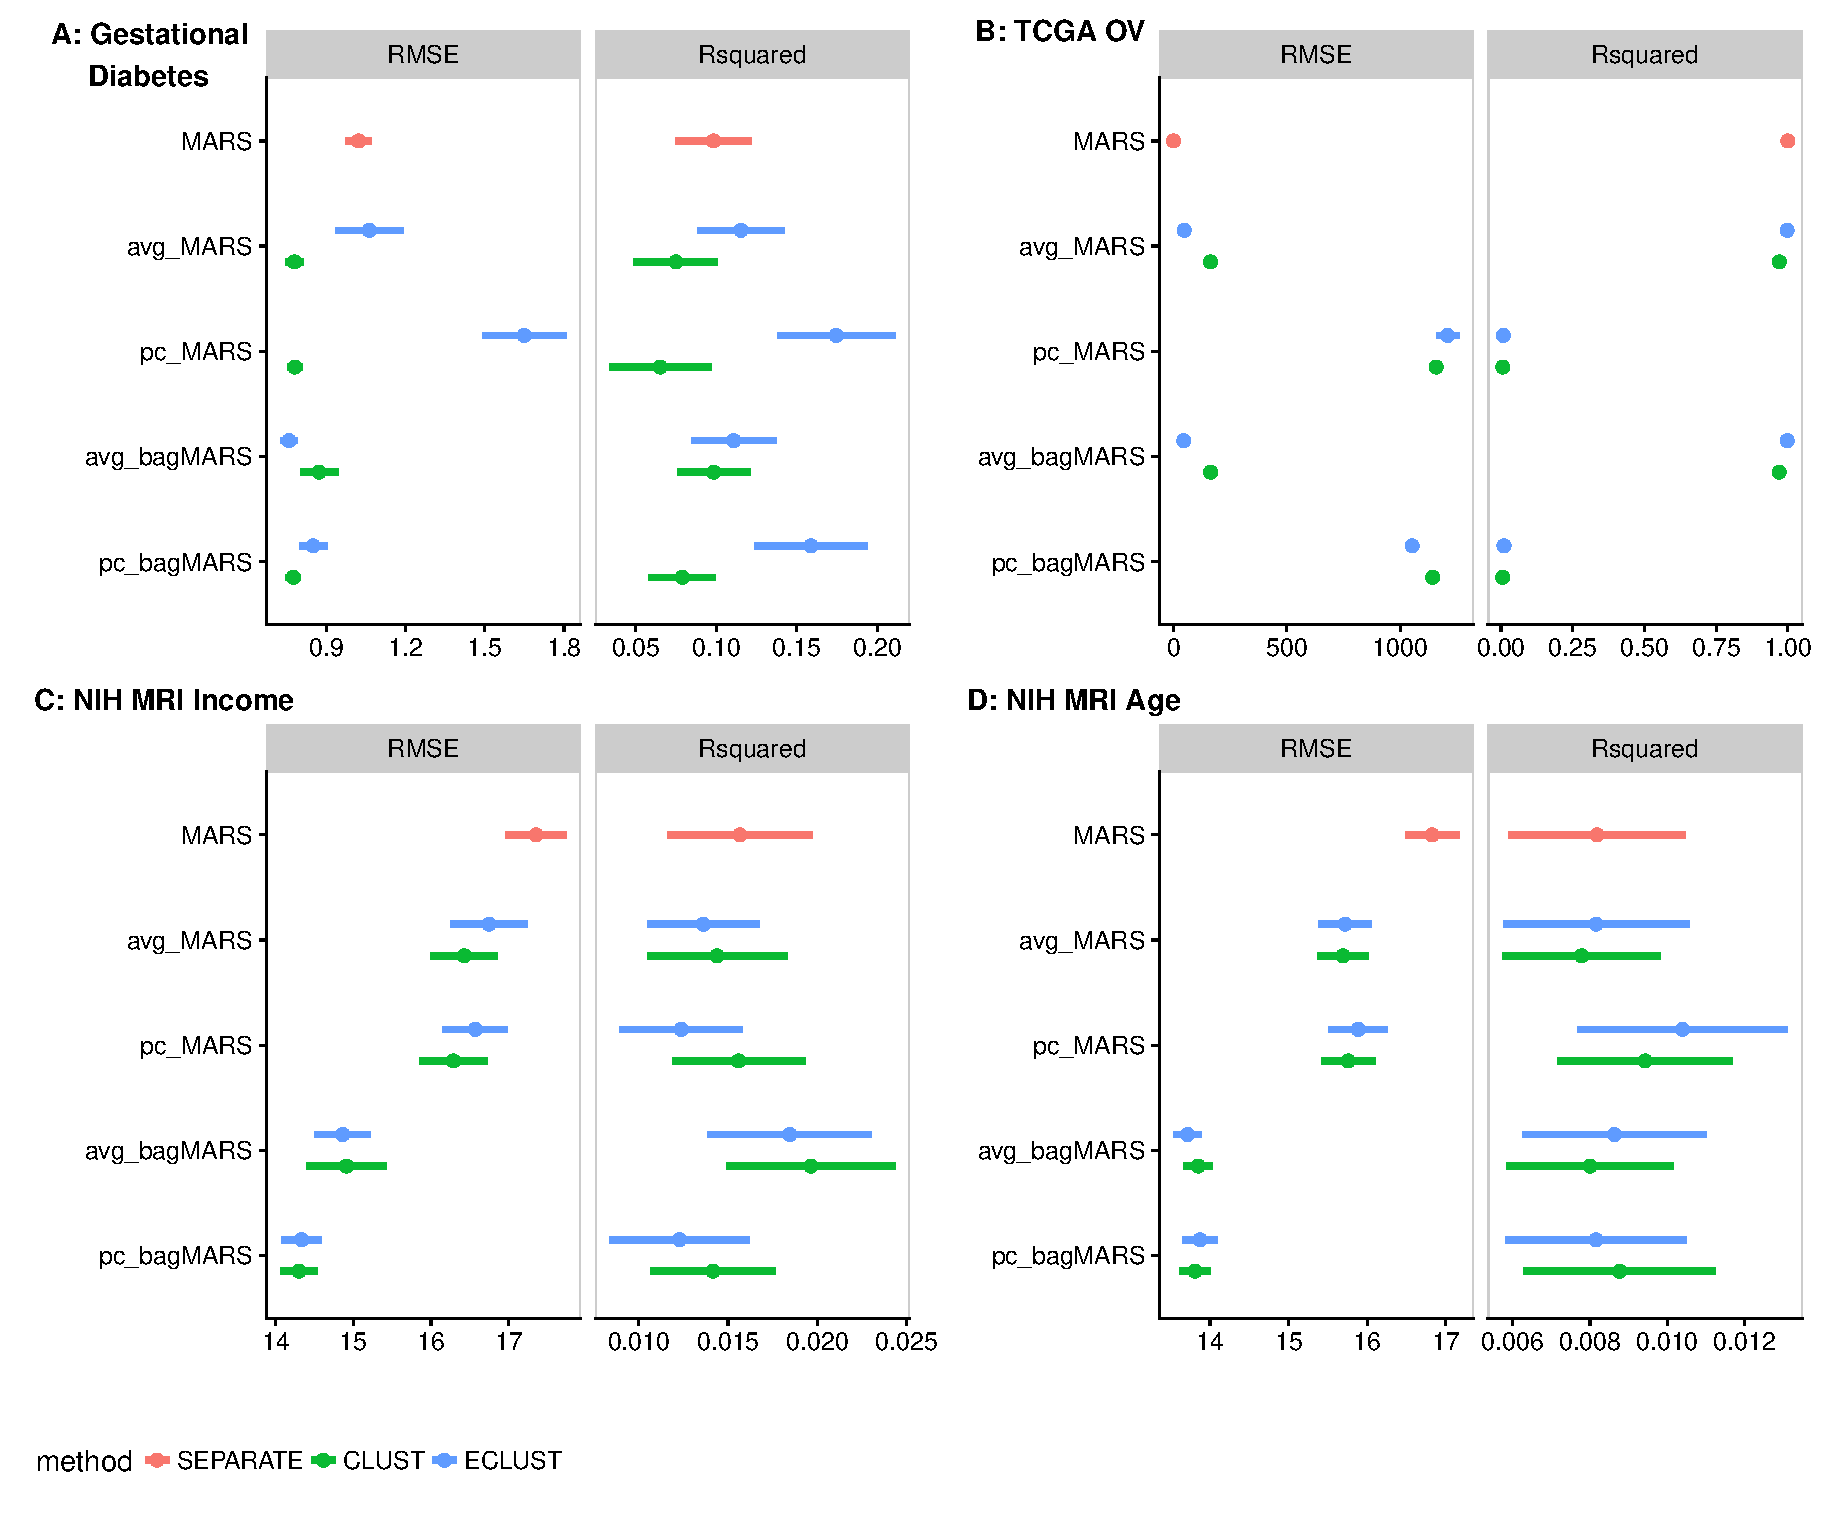
\includegraphics[scale=0.50, keepaspectratio]{figure7.eps}
	%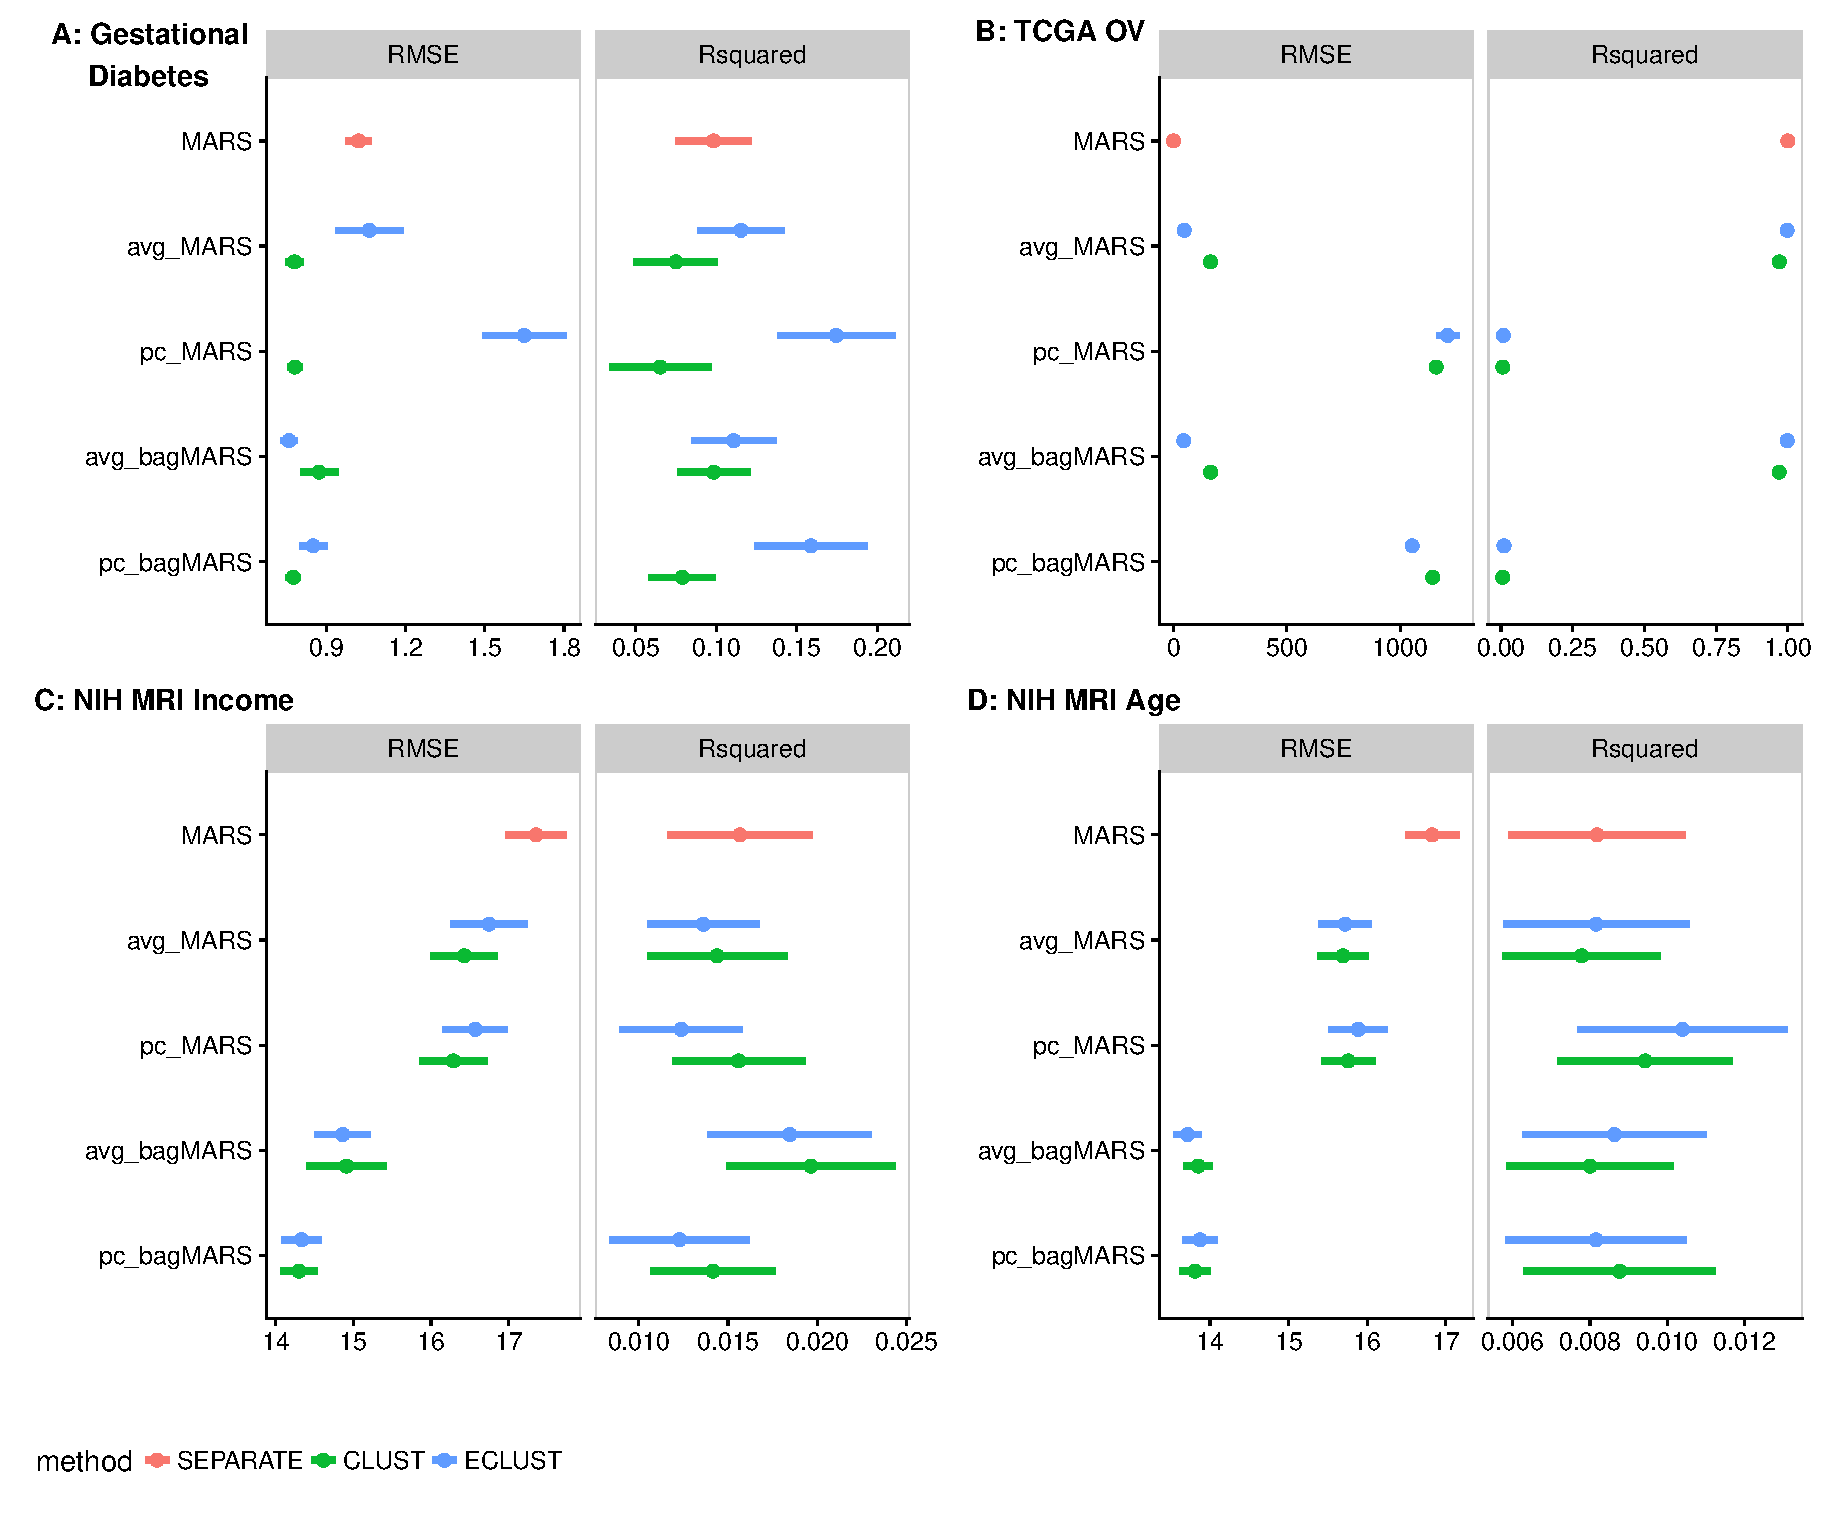
\includegraphics[]{figure7.eps}
	\caption{Model fit measures from analysis of three data sets: (A) Gestational diabetes birth-cohort (B) TCGA Ovarian Cancer study (C) NIH MRI Study with income as the environment variable (D) NIH MRI Study with age as the environment variable}
	\label{fig:rda}
\end{figure}
\end{comment}

\fig{figure7}{rda}{16cm}{Model fit measures from analysis of three data sets: (A) Gestational diabetes birth-cohort (B) TCGA Ovarian Cancer study (C) NIH MRI Study with income as the environment variable (D) NIH MRI Study with age as the environment variable.}{Model fit measures from analysis of three real data sets.}

The probes in these clusters mapped to 164 genes and these genes were selected to conduct pathway analyses using the Ingenuity Pathway Analysis (IPA) software (Ingenuity System). IPA compares the selected genes to a reference list of genes included in many biological pathways using a hypergeometric test. Smaller $p$ values are evidence for over-represented gene ontology categories in the input gene list. The results are summarized in Table~\ref{tab:ipa} and provide some biological validation of our ECLUST method. For example, the Hepatic system is involved with the metabolism of glucose and lipids~\citep{saltiel2001insulin}, and behavior and neurodevelopment are associated with obesity~\citep{epstein2004effect}. Furthermore, it is interesting that embryonic and organ development pathways are involved since GDM is associated with macrosomia~\citep{ehrenberg2004influence}. 

\begin{table}[h]	
	\begin{threeparttable}
		\caption{Ingenuity Pathway Analysis Results -- top-ranked diseases and disorders, and physiological system development and function epigentically affected by gestational diabetes mellitus and associated with childhood body mass index}
		\label{tab:ipa}
		\begin{tabulary}{\linewidth}{llll}
			\toprule
			Category              & Name & $p$ values & $n$\tabfnm{a} \\ \midrule
			%		General Approach              & Summary Measure &  Description\tabfnm{a,b} \\ 
			%			 & of Feature Clusters & \\ \midrule
			Diseases and Disorders       & Hepatic System Disease  & [\num{9.61e-07} -- \num{5.17e-07}] & 75 \\ \midrule
			\multicolumn{1}{m{5cm}}{Physiological System Development and Function} &   &  & \\
			& \multicolumn{1}{m{6cm}}{Behavior}  & [\num{1.35e-02} -- \num{7.82e-08}] & 33\\
			& \multicolumn{1}{m{6cm}}{Embryonic Development}  & [\num{1.35e-02} -- \num{2.63e-08}] & 26  \\
			& \multicolumn{1}{m{6cm}}{Nervous System Development and Function}  &[ \num{1.35e-02} -- \num{2.63e-08}] & 43  \\
			& \multicolumn{1}{m{6cm}}{Organ Development}  & [\num{1.35e-02} -- \num{2.63e-08}] & 20  \\
			& \multicolumn{1}{m{6cm}}{Organismal Development}  & [\num{1.35e-02} -- \num{2.63e-08}] & 34  \\ \bottomrule
		\end{tabulary}
		\begin{tablenotes}[para,flushleft]
			{\footnotesize
				%\textit{Note.} sfs
				\tabfnt{a}number of genes involved in each pathway
				
			}
		\end{tablenotes} 		
	\end{threeparttable}
\end{table}	

\section{Discussion}

The challenge of precision medicine is to appropriately fit treatments or recommendations to each individual.  Data such as gene expression, DNA methylation levels, or magnetic resonance imaging (MRI) signals are examples of HD measurements that capture multiple aspects of how a tissue is functioning. These data often show patterns associated with disease, and major investments are being made in the genomics research community to generate such HD data. Analytic tools increasing prediction accuracy are needed to maximize the productivity of these investments. However, the effects of exposures have usually been overlooked, but these are crucial since they can lead to ways to intervene. %{\color{red}.  To leave this sentence here, it would need to be cited.  But it may not belong here.  For example, gestational diabetes has been associated with altered methylation levels in placenta and cord blood, and GD is also known to lead to increased risks of overweight in offspring leading to life-long risks of morbidity}. 
Hence, it is essential to have a clear understanding of how exposures modify HD measures, and how the combination leads to disease. Existing methods for prediction (of disease), that are based on HD data and interactions with exposures, fall far short of being able to obtain this clear understanding. Most methods have low power and poor interpretability, and furthermore, modelling and interpretation problems are exacerbated when there is interest in interactions. In general, power to estimate interactions is low, and the number of possible interactions could be enormous. Therefore, here we have proposed a strategy to leverage situations where a covariate (e.g. an exposure) has a wide-spread effect on one or more HD measures, e.g. GDM on methylation levels. We have shown that this expected pattern can be used to construct dimension-reduced predictor variables that inherently capture the systemic covariate effects. These dimension-reduced variables, constructed without using the phenotype, can then be used in predictive models of any type.   In contrast to some common analysis strategies that model the effects of individual predictors on outcome, our approach makes a step towards a systems-based perspective that we believe will be more informative when exploring the factors that are associated with disease or a phenotype of interest. We have shown, through simulations and real data analysis, that incorporation of environmental factors into predictive models in a way that retains a high dimensional perspective can improve results and interpretation for both linear and non linear effects.

We proposed two key methodological steps necessary to maximize predictive model interpretability when using HD data and a binary exposure: (1) dimension reduction of HD data built on exposure sensitivity, and (2) implementation of penalized prediction models. In the first step, we proposed to identify exposure-sensitive HD pairs by contrasting the TOM between exposed and unexposed individuals; then we cluster the elements in these HD pairs to find exposure-sensitive co-regulated sets. New dimension-reduced variables that capture exposure-sensitive features (e.g. the first principal component of each cluster) were then defined. In the second step we implemented linear and non-linear variable selection methods using the dimension-reduced variables to ensure stability of the predictive model. The ECLUST method has been implemented in the \texttt{eclust}~\citep{eclust} R package publicly available on CRAN. Our method along with computationally efficient algorithms, allows for the analysis of up to 10,000 variables at a time on a laptop computer.

%{\color{red} Need a bit of discussion on correlations versus TOM - the performance of ECLUST being worse with correlations.  I think this speaks to the potential of developing a better measure than the difference of two matrices.  Also perhaps some discussion of first PC/average/ other choices.}


The methods that we have proposed here are currently only applicable when three data elements are available. Specifically a binary environmental exposure, a high dimensional dataset that can be affected by the exposure, and a single phenotype. When comparing the TOM and Pearson correlations as a measure of similarity, our simulations showed that the performance of ECLUST was worse with correlations. This speaks to the potential of developing a better measure than the difference of two matrices. For example, we are currently exploring ways in which to handle continuous exposures or multiple exposures. The best way to construct an exposure-sensitive distance matrix that can be used for clustering is not obvious in these situations. One possible solution relies on a non-parametric smoothing based approach where weighted correlations are calculated. These weights can be derived from a kernel-based summary of the exposure covariates (e.g.~\citep{qiu2016joint}). Then, contrasting unweighted and weighted matrices will allow construction of covariate-sensitive clusters. The choice of summary measure for each cluster also warrants further study. While principal components and averages are well understood and easy to implement, the main shortcoming is that they involve all original variables in the group. As the size of the groups increase, the interpretability of these measures decreases. Non-negative matrix factorization~\citep{lee2001algorithms} and sparse principal component analysis (SPCA)~\citep{witten2009penalized} are alternatives which find sparse and potentially interpretable factors. Furthermore, structured SPCA~\citep{jenatton2009structured} goes beyond restricting the cardinality of the contributing factors by imposing some a priori structural constraints deemed relevant to model the data at hand.





We are all aware that our exposures and environments impact our health and risks of disease, however detecting how the environment acts is extremely difficult.   Furthermore, it is very challenging to develop reliable and understandable ways of predicting the risk of disease in individuals, based on high dimensional data such as genomic or imaging measures, and this challenge is exacerbated when there are environmental exposures that lead to many subtle alterations in the genomic measurements.  Hence, we have developed an algorithm and an easy-to use software package to transform analysis of how environmental exposures impact human health, through an innovative signal-extracting approach for high dimensional measurements.  Evidently, the model fitting here is performed using existing methods; our goal is to illustrate the potential of improved dimension reduction in two-stage methods, in order to generate discussion and new perspectives.   
If such an approach can lead to more interpretable results that identify gene-environment interactions and their effects on diseases and traits,  the resulting understanding of how exposures influence the high-volume measurements now available in precision medicine will have important implications for health management and drug discovery.  
%(fine for a grant but over the top here, I think) Indeed, since exposures may be modifiable - this avenue provides the most plausible approach to developing helpful interventions, whether through drug treatments or lifestyle modifications. 

\section*{Availability of data and material}
%The data sets supporting the results of this article are available in the repositories:
\begin{enumerate}
	\item NIH MRI Study of Normal Brain Development data are available in the Pediatric MRI Data Repository, https://pediatricmri.nih.gov/
	\item Gene Expression Study of Ovarian Cancer data are available in the Genomic Data Commons repository, https://gdc.cancer.gov/, and were downloaded via the TCGA2STAT R library~\citep{tcga2stat}
	\item Gestational diabetes, epigenetics and metabolic disease: the clinical data, similarity matrices and cluster summaries are available at Zenodo [10.5281/zenodo.259222]. The raw analysed during the current study are not publicly available due to reasons of confidentiality, although specific collaborations with LB can be requested.
\end{enumerate}

\section*{Competing interests}
The authors declare that they have no competing interests.

\section*{Author's contributions}
SRB, CMTG, YY, MB: conceptualization; SRB, LB, BK: data curation; SRB: formal analysis, software, visualization; SRB, CMTG: methodology; SRB, CMTG: writing-original draft; SRB, CMTG, YY, BK, ACE, MB, LB: writing-review \& editing. 

\section*{Acknowledgements}
SRB was supported by the Ludmer Centre for Neuroinformatics and Mental Health.

\section*{Additional Files}
\subsection*{Additional file 1 -- Supplemental Methods and Simulation Results}
Contains the following sections:
\begin{itemize}
	\item[A] \textbf{Description of Topological Overlap Matrix} -  detailed description of the TOM
	\item[B] \textbf{Binary Outcome Simulation Results} - results of simulations 4, 5 and 6
	\item[C] \textbf{Analysis of Clusters} - number of estimated clusters by different measures of similarity	
	\item[D] \textbf{Simulation Results Using TOM as a Measure of Similarity} - detailed simulation results using TOM as a measure of similarity
	\item[E] \textbf{Simulation Results Using Pearson Correlations as a Measure of
		Similarity} - detailed simulation results using Pearson Correlations as a measure of similarity	
	\item[F] \textbf{Visual Representation of Similarity Matrices} - similarity matrices based on Pearson's correlation coefficient
	
\end{itemize}

	%-----------------------------------------------------------------------------
\chapter{Conclusion\label{ch:conclusion}}
%-----------------------------------------------------------------------------

\section{Summary}
The three manuscripts (Chapters~\ref{ch:sail},~\ref{ch:ggmix} and~\ref{ch:eclust}) presented in this thesis describe a body of work all within the context of penalized regression methods for interactions and mixed-effects models in high-dimensional data analysis. 


\section{Future work}



\section{Concluding remarks}
	\begin{appendices}


\chapter{Supplemental Methods and Simulation Results for Chapter~\ref{ch:sail}} \label{ap:sail}
\captionsetup{list=no}

\section{Algorithm Details} \label{ap:sail_algorithm}

In this section we provide more specific details about the algorithms used to solve the \sail ~objective function. 

\subsection{Least-Squares \sail ~with Strong Heredity} \label{ap:subsec:lssail}
A more detailed algorithm for fitting the least-squares \texttt{sail} model with strong heredity is given in Algorithm~\ref{alg:lssail}.

%\begin{comment}
%content...

\begin{algorithm}
	\caption{Blockwise Coordinate Descent for Least-Squares \texttt{sail} with Strong Heredity}\label{alg:lssail}
	\begin{algorithmic}[1]
		 %\algsetup{linenosize=\tiny}
		\small
		\Function{\texttt{sail}}{$\boldsymbol{X},Y, X_E,\texttt{basis},\lambda, \alpha,w_j, w_E, w_{jE}, \epsilon$}\Comment{Algorithm for solving~\eqref{eq:objective_least-squares}}
		%\State $\Psi_j \gets $ \texttt{splines::bs}($X_j$, \texttt{df}, \texttt{degree}) for $j=1, \ldots, p$
		%\State $\widetilde\Psi_j \gets X_E \circ \Psi_j$ for $j=1, \ldots, p$
		\State $\Psi_j \gets $ \texttt{basis}($X_j$), $\widetilde\Psi_j \gets X_E \circ \Psi_j$ for $j=1, \ldots, p$
		%\item[]
		\State Initialize: $\beta_0^{(0)}\gets \bar{Y}$, $\beta_E^{(0)}=\btheta_j^{(0)}=\gamma_j^{(0)} \gets 0$ for $j=1, \ldots, p$.
		%\State Initialize: $R^\ast \gets Y $ %\Comment{Initial partial residual used for $\btheta$ update}
		\State Set iteration counter $k \gets 0$
		\State $R^\ast \gets Y - \beta_0^{(k)} - \beta_E^{(k)} X_E - \sum_{j}  (\bPsi_{j} + \gamma_{j}^{(k)} \beta_E^{(k)}  \widetilde\bPsi_{j}) \btheta_{j}^{(k)}$
		\Repeat		
		\State $\bullet$ To update $\boldsymbol{\gamma}=(\gamma_1, \ldots, \gamma_p)$
		\Indent
		\State $\widetilde{X}_j \gets \beta_E^{(k)} \widetilde{\bPsi}_j \btheta_j^{(k)} \qquad$ for $j = 1, \ldots, p$
		\State $R \gets R^\ast + \sum_{j=1}^p  \gamma_{j}^{(k)} \widetilde{X}_j$
		%\State $R_1 \gets Y - \beta_0^{(k)} - \beta_E^{(k)} X_E - \sum_{j} \bPsi_j \btheta_j^{(k)}$
		\State \[\boldsymbol{\gamma}^{(k)(new)} \gets \argmin_{\boldsymbol{\gamma}} \frac{1}{2n} \norm{R - \sum_{j} \gamma_j \widetilde{X}_j}_2^2 + \lambda \alpha \sum_{j} w_{jE} \abs{\gamma_{j}}\]
		\State $\Delta = \sum_j (\gamma_j^{(k)} - \gamma_j^{(k)(new)}) \widetilde{X}_j $
		\State $R^\ast \gets R^\ast + \Delta$
		\EndIndent
		\State $\bullet$ To update $\btheta = (\btheta_1, \ldots, \btheta_p)$
		\Indent
		\State %$\beta_0^{(k)} \gets \beta_0^{(k-1)}$, $\btheta_j^{(k)} \gets \btheta_j^{(k-1)}$, 
		$\widetilde{X}_j \gets \bPsi_j + \gamma_{j}^{(k)} \beta_E^{(k)} \widetilde\bPsi_{j}$ for $j=1, \ldots, p$
		\For{$j=1, \ldots, p$}
		\State $R \gets R^\ast + \widetilde{X}_j\btheta_j^{(k)}$
		%\State $R_2 \gets Y - \beta_0^{(k)} - \beta_E^{(k)} X_E - \sum_{j=1}^p  (\bPsi_{j} + \gamma_{j}^{(k)} \beta_E^{(k)}  \widetilde\bPsi_{j}) \btheta_{j}^{(k)} + (\bPsi_j + \gamma_j^{(k)}\beta_E^{(k)} \widetilde{\bPsi}_j)\btheta_j^{(k)}$
		%\If{$j=1$} \State $\Delta \gets 0$ \Else \State $\Delta \gets \widetilde{X}_{j}  \btheta_{j}^{(k)} - \widetilde{X}_{j-1} \btheta_{j-1}^{(k)}$ \Comment{see~\eqref{subsec:Delta} for details}
		%\EndIf
		%\State $R_2 \gets R_2 + \Delta$
		\State \[\btheta_j^{(k)(new)} \gets \argmin_{\btheta_j} \frac{1}{2n} \norm{R -  \widetilde{X}_j \btheta_j}_2^2 + \lambda (1-\alpha) w_j \norm{\theta_j}_2\]
		%\State $R_2^{\prime\prime} \gets Y - \beta_0^{(k)} - \beta_E^{(k)} X_E - \sum_{\ell \neq j}  \bPsi_{\ell} \btheta_{\ell}^{(k)} - \sum_{\ell \neq j} \gamma_{\ell}^{(k)} \beta_E^{(k)}  \widetilde\bPsi_{\ell} \btheta_{\ell}^{(k)} $
		\State $\Delta = \widetilde{X}_j(\btheta_j^{(k)} - \btheta_j^{(k)(new)})$
		\State $R^\ast \gets R^\ast + \Delta$
		\EndFor 
		\EndIndent
		%\item[]
		\State $\bullet$ To update $\beta_E$
		\Indent
		\State $\widetilde{X}_E \gets X_E + \sum_{j} \gamma_j^{(k)} \widetilde\bPsi_j \btheta_j^{(k)}$
		%\State $R \gets R^\ast + \beta_E^{(k)} X_E + \sum_{j}  ( \gamma_{j}^{(k)} \beta_E^{(k)}  \widetilde\bPsi_{j}) \btheta_{j}^{(k)} = R^\ast + \beta_E^{(k)} \widetilde{X}_E$
		\State $R \gets R^\ast + \beta_E^{(k)} \widetilde{X}_E$
		%\State $R_3 \gets Y - \beta_0^{(k)} - \sum_j \bPsi_j \btheta_j^{(k)} - \sum_{j} \gamma_j^{(k)}  \bPsi_j \btheta_j^{(k)}$
		\State \[\beta_E^{(k)(new)} \gets S\left(\frac{1}{n \cdot w_E} \widetilde{X}_E^\top R, \lambda(1-\alpha)\right)\] \Comment{$S(x,t) = \textrm{sign}(x) (\abs{x} - t)_+$}
		%\State $\beta_E^{(k)} \gets \argmin_{\beta_E} \frac{1}{2n} \norm{R_3 - \beta_E \widetilde{X}_E}_2^2 + \lambda(1-\alpha) w_E \abs{\beta_E}$
		\State $\Delta = (\beta_E^{(k)} - \beta_E^{(k)(new)})\widetilde{X}_E$
		\State $R^\ast \gets R^\ast + \Delta$
		\EndIndent
		\State $\bullet$ To update $\beta_0$
		\Indent
		\State $R \gets R^* + \beta_0^{(k)}$
		%\State $R_4 \gets Y - \beta_E^{(k)} X_E - \sum_{j}  \bPsi_{j} \btheta_{j}^{(k)} - \sum_{j} \gamma_{j}^{(k)} \beta_E^{(k)}  \widetilde\bPsi_{j} \btheta_{j}^{(k)}$ 
		\State \[\beta_0^{(k)(new)} \gets \frac{1}{n} R^\ast \cdot \boldsymbol{1}\]
		\State $\Delta = \beta_0^{(k)} - \beta_0^{(k)(new)}$
		\State $R^\ast \gets R^\ast + \Delta$
		\EndIndent
		\State $k \gets k + 1$
		%\State \Until{convergence criterion is satisfied: $\norm{\bTheta^{(k)} - \bTheta^{(k-1)}}_2^2 < \epsilon$}
		\State \Until{convergence criterion is satisfied: $\abs{Q(\bTheta^{(k-1)}) - Q(\bTheta^{(k)})} /Q(\bTheta^{(k-1)})  < \epsilon$}
		\EndFunction
\end{algorithmic}
\end{algorithm}

%\end{comment}

\newpage


\subsection{Details on Update for $\btheta$} \label{ap:subsec:Delta}

Here we discuss a computational speedup in the updates for the $\btheta$ parameter. The partial residual ($R_{s}$) used for updating $\btheta_s$ ($s \in {1,\ldots, p}$) at the $k$th iteration is given by
\begin{align}
R_{s} & = Y - \widetilde{Y}_{(-s)}^{(k)} \label{eq:r2}
\end{align}
where $\widetilde{Y}_{(-s)}^{(k)}$ is the fitted value at the $k$th iteration excluding the contribution from $\bPsi_s$:
\begin{align}
\widetilde{Y}_{(-s)}^{(k)} & = \beta_0^{(k)} - \beta_E^{(k)} X_E - \sum_{\ell \neq s}  \bPsi_{\ell} \btheta_{\ell}^{(k)} - \sum_{\ell \neq s} \gamma_{\ell}^{(k)} \beta_E^{(k)}  \widetilde\bPsi_{\ell} \btheta_{\ell}^{(k)} \label{eq:r2_2}
\end{align}
Using~\eqref{eq:r2_2},~\eqref{eq:r2} can be re-written as
\begin{align}
% R_2 & = Y - \beta_0^{(k)} - \beta_E^{(k)} X_E - \sum_{j=1}^p  \bPsi_{j} \btheta_{j}^{(k)} - \sum_{j=1}^p \gamma_{j}^{(k)} \beta_E^{(k)}  \widetilde\bPsi_{j} \btheta_{j}^{(k)} + (\bPsi_s + \gamma_s^{(k)}\beta_E^{(k)} \widetilde{\bPsi}_s)\btheta_s^{(k)}  \\
R_{s} & = Y - \beta_0^{(k)} - \beta_E^{(k)} X_E - \sum_{j=1}^p  (\bPsi_{j} + \gamma_{j}^{(k)} \beta_E^{(k)}  \widetilde\bPsi_{j}) \btheta_{j}^{(k)} + (\bPsi_s + \gamma_s^{(k)}\beta_E^{(k)} \widetilde{\bPsi}_s)\btheta_s^{(k)} \nonumber \\
& = R^\ast + (\bPsi_s + \gamma_s^{(k)}\beta_E^{(k)} \widetilde{\bPsi}_s)\btheta_s^{(k)} \label{eq:r2_3} 
\end{align}
where 
\begin{equation}
R^\ast = Y - \beta_0^{(k)} - \beta_E^{(k)} X_E - \sum_{j=1}^p  (\bPsi_{j} + \gamma_{j}^{(k)} \beta_E^{(k)}  \widetilde\bPsi_{j}) \btheta_{j}^{(k)} \label{eq:rast}
\end{equation}
Denote $\btheta_{s}^{(k)(\tm{new})}$ the solution for predictor $s$ at the $k$th iteration, given by:
\begin{align}
\btheta_s^{(k)(new)} = \argmin_{\btheta_j} \frac{1}{2n} \norm{R_s - (\bPsi_s + \gamma_{s}^{(k)} \beta_E^{(k)}\widetilde{\bPsi}_{s})\btheta_j }_2^2 + \lambda (1-\alpha) w_s \norm{\theta_j}_2 \label{eq:r2_4}
\end{align}
Now we want to update the parameters for the next predictor $\btheta_{s+1}$ ($s+1 \in {1,\ldots, p}$) at the $k$th iteration. The partial residual used to update $\btheta_{s+1}$ is given by
\begin{align}
R_{s+1} & = R^\ast + (\bPsi_{s+1} + \gamma_{s+1}^{(k)}\beta_E^{(k)} \widetilde{\bPsi}_{s+1})\btheta_{s+1}^{(k)} + (\bPsi_s + \gamma_s^{(k)}\beta_E^{(k)} \widetilde{\bPsi}_s)(\btheta_s^{(k)} - \btheta_s^{(k)(new)}) \label{eq:r2_5} 
\end{align}
where $R^\ast$ is given by~\eqref{eq:rast}, $\btheta_s^{(k)}$ is the parameter value prior to the update, and $\btheta_s^{(k)(new)}$ is the updated value given by~\eqref{eq:r2_4}. Taking the difference between~\eqref{eq:r2_3} and~\eqref{eq:r2_5} gives
\begin{align}
\Delta & = R_t - R_s \nonumber\\
& = (\bPsi_t + \gamma_t^{(k)}\beta_E^{(k)} \widetilde{\bPsi}_t)\btheta_t^{(k)} + (\bPsi_s + \gamma_s^{(k)}\beta_E^{(k)} \widetilde{\bPsi}_s)(\btheta_s^{(k)} - \btheta_s^{(k)(new)}) - (\bPsi_s + \gamma_s^{(k)}\beta_E^{(k)} \widetilde{\bPsi}_s)\btheta_s^{(k)} \nonumber\\
& = (\bPsi_t + \gamma_t^{(k)}\beta_E^{(k)} \widetilde{\bPsi}_t)\btheta_t^{(k)} - (\bPsi_s + \gamma_s^{(k)}\beta_E^{(k)} \widetilde{\bPsi}_s)\btheta_s^{(k)(new)} \label{eq:Delta}
\end{align} 
Therefore $R_t = R_s + \Delta$, and the partial residual for updating the next predictor can be computed by updating the previous partial residual by $\Delta$, given by~\eqref{eq:Delta}. This formulation can lead to computational speedups especially when $\Delta = 0$, meaning the partial residual does not need to be re-calculated.  



\subsection{Least-Squares \sail ~with Weak Heredity} \label{ap:subsec:lssailweak}

The least-squares \texttt{sail} model with weak heredity has the form
\begin{equation}
\hat{Y}   =  \beta_0 \cdot \boldsymbol{1} + \sum_{j=1}^p \bPsi_j \btheta_j + \beta_E X_E + \sum_{j=1}^p \gamma_{j}  (X_E \circ \bPsi_j) (\beta_E\cdot \mb{1}_{m_j} + \btheta_j)
\end{equation}
The objective function is given by 
\begin{equation}
Q(\bTheta) = \frac{1}{2n} \norm{Y - \hat{Y}}_2^2 + \lambda (1-\alpha)  \left( w_E \abs{\beta_E} + \sum_{j=1}^{p} w_j \norm{\btheta_j}_2 \right) +  \lambda\alpha \sum_{j=1}^{p} w_{jE} \abs{\gamma_{j}} \label{eq:objective_least-squares-weak}
\end{equation}
Denote the $n$-dimensional residual column vector $R = Y-\hat{Y}$. The subgradient equations are given by
\begin{align}
\frac{\partial Q}{\partial \beta_0} & = \frac{1}{n} \left( Y - \beta_0 \cdot \boldsymbol{1} - \sum_{j=1}^p \bPsi_j \btheta_j - \beta_E X_E - \sum_{j=1}^p \gamma_{j}  (X_E \circ \bPsi_j)(\beta_E \cdot \mb{1}_{m_j} + \btheta_j)\right)^\top \boldsymbol{1}  = 0 \label{eq:sub_b0_weak} \\
\frac{\partial Q}{\partial \beta_E} & = -\frac{1}{n} \left(X_E + \sum_{j=1}^{p}\gamma_j (X_E \circ \bPsi_j)\mb{1}_{m_j}\right)^\top R  + \lambda (1-\alpha) w_E s_1 = 0 \label{eq:sub_bEweak}\\
\frac{\partial Q}{\partial \btheta_j} & = -\frac{1}{n} \left(\bPsi_j + \gamma_j (X_E \circ \bPsi_j)\right)^\top R  + \lambda (1-\alpha) w_j s_2 = \boldsymbol{0} \label{eq:sub_thetajweak}\\
\frac{\partial Q}{\partial \gamma_j} & = -\frac{1}{n} \left((X_E \circ \bPsi_j)(\beta_E \cdot \mb{1}_{m_j} + \btheta_j)\right)^\top R  + \lambda \alpha w_{jE} s_3 = 0 \label{eq:sub_gammajweak}
\end{align}
where $s_1$ is in the subgradient of the $\ell_1$ norm:
$$
s_1 \in \begin{cases}
\textrm{sign}\left(\beta_E\right) & \tm{if  } \beta_E \neq 0\\
[-1, 1] &  \tm{if  } \beta_E = 0,\\
\end{cases}
$$
$s_2$ is in the subgradient of the $\ell_2$ norm:
$$
s_2 \in \begin{cases}
\dfrac{\btheta_j}{\norm{\btheta_j}_2} &  \tm{if  } \btheta_j \neq \boldsymbol{0}\\
u \in \mathbb{R}^{m_j}: \norm{u}_2 \leq 1 & \tm{if  } \btheta_j = \boldsymbol{0},\\
\end{cases}
$$
and $s_3$ is in the subgradient of the $\ell_1$ norm:
$$
s_3 \in \begin{cases}
\textrm{sign}\left(\gamma_j\right) & \tm{if  } \gamma_j \neq 0\\
[-1, 1] &  \tm{if  } \gamma_j = 0.\\
\end{cases}
$$
Define the partial residuals, without the $j$th predictor for $j=1, \ldots, p$, as
\[R_{(-j)} = Y - \beta_0 \cdot \boldsymbol{1} - \sum_{\ell \neq j} \bPsi_\ell \btheta_\ell - \beta_E X_E - \sum_{\ell\neq j} \gamma_{\ell}  (X_E \circ \bPsi_\ell) (\beta_E \cdot \mb{1}_{m_{\ell}} +\btheta_\ell) \]
the partial residual without $X_E$ as
\[R_{(-E)} = Y - \beta_0 \cdot \boldsymbol{1} - \sum_{j=1}^p \bPsi_j \btheta_j - \sum_{j=1}^p \gamma_{j}  (X_E \circ \bPsi_j) \btheta_j\]
and the partial residual without the $j$th interaction for $j=1, \ldots, p$
\[R_{(-jE)} = Y - \beta_0 \cdot \boldsymbol{1} - \sum_{j=1}^p \bPsi_j \btheta_j - \beta_E X_E - \sum_{\ell\neq j} \gamma_{\ell} (X_E \circ \bPsi_\ell) (\beta_E \cdot \mb{1}_{m_{\ell}} +\btheta_\ell) \]
From the subgradient Equation~\eqref{eq:sub_bEweak}, we see that $\beta_E = 0$ is a solution if
\begin{equation}
\frac{1}{w_E}\abs{\frac{1}{n} \left(X_E + \sum_{j=1}^{p}\gamma_j (X_E \circ \bPsi_j)\mb{1}_{m_j}\right)^\top R_{(-E)}} \leq \lambda (1-\alpha)
\end{equation}
From the subgradient Equation~\eqref{eq:sub_thetajweak}, we see that $\btheta_j = \boldsymbol{0}$ is a solution if
\begin{equation}
\frac{1}{w_{j}}\norm{\frac{1}{n} \left(\bPsi_j + \gamma_j (X_E \circ \bPsi_j)\right)^\top R_{(-j)}}_2 \leq \lambda (1-\alpha)
\end{equation}
From the subgradient Equation~\eqref{eq:sub_gammajweak}, we see that $\gamma_j = 0$ is a solution if
\begin{equation}
\frac{1}{w_{jE}}\abs{\frac{1}{n} \left((X_E \circ \bPsi_j)(\beta_E \cdot \mb{1}_{m_j}+\btheta_j)\right)^\top R_{(-jE)}} \leq \lambda \alpha
\end{equation}
From the subgradient equations we see that 
\begin{align}
\hat{\beta}_0 &=  \left( Y - \sum_{j=1}^p \bPsi_j \hat\btheta_j - \hat\beta_E X_E - \sum_{j=1}^p \hat\gamma_{j}   (X_E \circ \bPsi_j)(\hat\beta_E\cdot \mb{1}_{m_j}+ \hat\btheta_j)\right)^\top \boldsymbol{1} \\
\hat{\beta}_E & = S\left(\frac{1}{n \cdot w_E} \left(X_E + \sum_{j=1}^{p}\hat\gamma_j (X_E \circ \bPsi_j)\mb{1}_{m_j}\right)^\top R_{(-E)}, \lambda(1-\alpha)\right) \\
\lambda (1-\alpha) w_j \dfrac{\btheta_j}{\norm{\btheta_j}_2} & =  \frac{1}{n} \left(\bPsi_j + \gamma_j (X_E \circ \bPsi_j)\right)^\top R_{(-j)} \label{eq:thetajweak} \\
\hat\gamma_j & = S \left(\frac{1}{n \cdot w_{jE}} \left((X_E \circ \bPsi_j)(\beta_E \cdot \mb{1}_{m_j}+\btheta_j)\right)^\top R_{(-jE)}, \lambda \alpha\right)
\end{align}
where $S(x,t) = \textrm{sign}(x) (\abs{x} - t)$ is the soft-thresholding operator. As was the case in the strong heredity \sail ~model, there are closed form solutions for the intercept and $\beta_E$, each $\gamma_j$ also has a closed form solution and can be solved efficiently for $j=1, \ldots, p$ using the coordinate descent procedure implemented in the \texttt{glmnet} package~\citep{friedman2010regularization}, while we use the quadratic majorization technique implemented in the \texttt{gglasso} package~\citep{yang2015fast} to solve~\eqref{eq:thetajweak}. Algorithm~\ref{alg:sailweak} details the procedure used to fit the least-squares weak heredity \sail ~model.

%\begin{comment}
\begin{algorithm}
\caption{Coordinate descent for least-squares \texttt{sail} with weak heredity}\label{alg:sailweak}
\begin{algorithmic}[1]
\small
\Function{\texttt{sail}}{$\boldsymbol{X},Y, X_E,\texttt{basis},\lambda, \alpha,w_j, w_E, w_{jE}, \epsilon$}\Comment{Algorithm for solving~\eqref{eq:objective_least-squares-weak}}
\State $\Psi_j \gets $ \texttt{basis}($X_j$), $\widetilde\Psi_j \gets X_E \circ \Psi_j$ for $j=1, \ldots, p$
%\State  for $j=1, \ldots, p$
%\item[]
\State Initialize: $\beta_0^{(0)}\gets \bar{Y}$, $\beta_E^{(0)}=\btheta_j^{(0)} = \gamma_j^{(0)} \gets 0$ for $j=1, \ldots, p$.
%\State Initialize: $R^\ast \gets Y $ %\Comment{Initial partial residual used for $\btheta$ update}
\State Set iteration counter $k \gets 0$
\State $R^\ast \gets Y - \beta_0^{(k)} - \beta_E^{(k)} X_E - \sum_{j}  \bPsi_{j}\btheta_{j}^{(k)} - \sum_{j} \gamma_{j}^{(k)} \widetilde\bPsi_{j}(\beta_E^{(k)}\cdot \mb{1}_{m_j} +\btheta_{j}^{(k)})$
\Repeat		
\State $\bullet$ To update $\boldsymbol{\gamma}=(\gamma_1, \ldots, \gamma_p)$
\Indent
\State $\widetilde{X}_j \gets \widetilde{\bPsi}_j (\beta_E^{(k)}\cdot \mb{1}_{m_j}+ \btheta_j^{(k)}) \qquad$ for $j = 1, \ldots, p$
\State $R \gets R^\ast + \sum_{j=1}^p  \gamma_{j}^{(k)} \widetilde{X}_j$
%\State $R_1 \gets Y - \beta_0^{(k)} - \beta_E^{(k)} X_E - \sum_{j} \bPsi_j \btheta_j^{(k)}$
\State \[\boldsymbol{\gamma}^{(k)(new)} \gets \argmin_{\boldsymbol{\gamma}} \frac{1}{2n} \norm{R - \sum_{j} \gamma_j \widetilde{X}_j}_2^2 + \lambda \alpha \sum_{j} w_{jE} \abs{\gamma_{j}}\]
\State $\Delta = \sum_j (\gamma_j^{(k)} - \gamma_j^{(k)(new)}) \widetilde{X}_j $
\State $R^\ast \gets R^\ast + \Delta$
\EndIndent
\State $\bullet$ To update $\btheta = (\btheta_1, \ldots, \btheta_p)$
\Indent
\State %$\beta_0^{(k)} \gets \beta_0^{(k-1)}$, $\btheta_j^{(k)} \gets \btheta_j^{(k-1)}$, 
$\widetilde{X}_j \gets \bPsi_j + \gamma_{j}^{(k)} \widetilde\bPsi_{j}$ for $j=1, \ldots, p$
\For{$j=1, \ldots, p$}
\State $R \gets R^\ast + \widetilde{X}_j\btheta_j^{(k)}$
%\State $R_2 \gets Y - \beta_0^{(k)} - \beta_E^{(k)} X_E - \sum_{j=1}^p  (\bPsi_{j} + \gamma_{j}^{(k)} \beta_E^{(k)}  \widetilde\bPsi_{j}) \btheta_{j}^{(k)} + (\bPsi_j + \gamma_j^{(k)}\beta_E^{(k)} \widetilde{\bPsi}_j)\btheta_j^{(k)}$
%\If{$j=1$} \State $\Delta \gets 0$ \Else \State $\Delta \gets \widetilde{X}_{j}  \btheta_{j}^{(k)} - \widetilde{X}_{j-1} \btheta_{j-1}^{(k)}$ \Comment{see~\eqref{subsec:Delta} for details}
%\EndIf
%\State $R_2 \gets R_2 + \Delta$
\State \[\btheta_j^{(k)(new)} \gets \argmin_{\btheta_j} \frac{1}{2n} \norm{R -  \widetilde{X}_j \btheta_j}_2^2 + \lambda (1-\alpha) w_j \norm{\theta_j}_2\]
%\State $R_2^{\prime\prime} \gets Y - \beta_0^{(k)} - \beta_E^{(k)} X_E - \sum_{\ell \neq j}  \bPsi_{\ell} \btheta_{\ell}^{(k)} - \sum_{\ell \neq j} \gamma_{\ell}^{(k)} \beta_E^{(k)}  \widetilde\bPsi_{\ell} \btheta_{\ell}^{(k)} $
\State $\Delta = \widetilde{X}_j(\btheta_j^{(k)} - \btheta_j^{(k)(new)})$
\State $R^\ast \gets R^\ast + \Delta$
\EndFor 
\EndIndent
%\item[]
\State $\bullet$ To update $\beta_E$
\Indent
\State $\widetilde{X}_E \gets X_E + \sum_{j} \gamma_j^{(k)} \widetilde\bPsi_j \mb{1}_{m_j}$
%\State $R \gets R^\ast + \beta_E^{(k)} X_E + \sum_{j}  ( \gamma_{j}^{(k)} \beta_E^{(k)}  \widetilde\bPsi_{j}) \btheta_{j}^{(k)} = R^\ast + \beta_E^{(k)} \widetilde{X}_E$
\State $R \gets R^\ast + \beta_E^{(k)} \widetilde{X}_E$
%\State $R_3 \gets Y - \beta_0^{(k)} - \sum_j \bPsi_j \btheta_j^{(k)} - \sum_{j} \gamma_j^{(k)}  \bPsi_j \btheta_j^{(k)}$
\State \[\beta_E^{(k)(new)} \gets S\left(\frac{1}{n \cdot w_E} \widetilde{X}_E^\top R, \lambda(1-\alpha)\right)\] \Comment{$S(x,t) = \textrm{sign}(x) (\abs{x} - t)_+$}
%\State $\beta_E^{(k)} \gets \argmin_{\beta_E} \frac{1}{2n} \norm{R_3 - \beta_E \widetilde{X}_E}_2^2 + \lambda(1-\alpha) w_E \abs{\beta_E}$
\State $\Delta = (\beta_E^{(k)} - \beta_E^{(k)(new)})\widetilde{X}_E$
\State $R^\ast \gets R^\ast + \Delta$
\EndIndent
\State $\bullet$ To update $\beta_0$
\Indent
\State $R \gets R^* + \beta_0^{(k)}$
%\State $R_4 \gets Y - \beta_E^{(k)} X_E - \sum_{j}  \bPsi_{j} \btheta_{j}^{(k)} - \sum_{j} \gamma_{j}^{(k)} \beta_E^{(k)}  \widetilde\bPsi_{j} \btheta_{j}^{(k)}$ 
\State \[\beta_0^{(k)(new)} \gets \frac{1}{n} R^\ast \cdot \boldsymbol{1}\]
\State $\Delta = \beta_0^{(k)} - \beta_0^{(k)(new)}$
\State $R^\ast \gets R^\ast + \Delta$
\EndIndent
\State $k \gets k + 1$
%\State \Until{convergence criterion is satisfied: $\norm{\bTheta^{(k)} - \bTheta^{(k-1)}}_2^2 < \epsilon$}
\State \Until{convergence criterion is satisfied: $\abs{Q(\bTheta^{(k-1)}) - Q(\bTheta^{(k)})} /Q(\bTheta^{(k-1)})  < \epsilon$}
\EndFunction
\end{algorithmic}
\end{algorithm}
%\end{comment}

\subsubsection{Lambda Max}

The smallest value of $\lambda$ for which the entire parameter vector $(\beta_E,\btheta_1, \ldots, \btheta_p, \gamma_1, \ldots, \gamma_p)$ is $\boldsymbol{0}$ is:

\begin{multline}
\lambda_{max} = \frac{1}{n} \max \left\lbrace \frac{1}{(1-\alpha)w_E}\left(X_E + \sum_{j=1}^{p}\gamma_j (X_E \circ \bPsi_j)\mb{1}_{m_j}\right)^\top R_{(-E)}, \right. \\
\left. \max_j \frac{1}{(1-\alpha)w_{j}}\norm{\left(\bPsi_j + \gamma_j (X_E \circ \bPsi_j)\right)^\top R_{(-j)}}_2, \right. \\
\left. \max_j \frac{1}{\alpha w_{jE}}\left((X_E \circ \bPsi_j)(\beta_E \cdot \mb{1}_{m_j}+\btheta_j)\right)^\top R_{(-jE)}  \right\rbrace 
\end{multline}
which reduces to
\begin{align*}
\lambda_{max} = \frac{1}{n(1-\alpha)} \max \left\lbrace \frac{1}{w_E}\left(X_E\right)^\top R_{(-E)}, \max_j \frac{1}{w_{j}}\norm{\left(\bPsi_j\right)^\top R_{(-j)}}_2   \right\rbrace 
\end{align*}

This is the same $\lambda_{max}$ as the least-squares strong heredity \sail ~model. 


\FloatBarrier 

\section{Simulation Results} \label{ap:simulation}



\begin{knitrout}\scriptsize
	\definecolor{shadecolor}{rgb}{0.969, 0.969, 0.969}\color{fgcolor}\begin{figure}[H]
		
		{\centering \includegraphics[width=1\linewidth]{figs/plot-mse-nactive-sim-1} 
			
		}
		
		\caption[Test set MSE vs number of active variables results]{Test set MSE vs number of active variables results.}\label{fig:plot-mse-nactive-sim}
	\end{figure}
	
	
\end{knitrout}


\begin{knitrout}\scriptsize
	\definecolor{shadecolor}{rgb}{0.969, 0.969, 0.969}\color{fgcolor}\begin{figure}[H]
		
		{\centering \includegraphics[width=1\linewidth]{figs/plot-tpr-sim-1} 
			
		}
		
		\caption[True positive rate results]{True positive rate results.}\label{fig:plot-tpr-sim}
	\end{figure}
	
	
\end{knitrout}

\begin{knitrout}\scriptsize
	\definecolor{shadecolor}{rgb}{0.969, 0.969, 0.969}\color{fgcolor}\begin{figure}[H]
		
		{\centering \includegraphics[width=1\linewidth]{figs/plot-fpr-sim-1} 
			
		}
		
		\caption[False positive rate results]{False positive rate results.}\label{fig:plot-fpr-sim}
	\end{figure}
	
	
\end{knitrout}

\begin{knitrout}\scriptsize
	\definecolor{shadecolor}{rgb}{0.969, 0.969, 0.969}\color{fgcolor}\begin{figure}[H]
		
		{\centering \includegraphics[width=1\linewidth]{figs/plot-nactive-sim-1} 
			
		}
		
		\caption[Number of active variables results]{Number of active variables results.}\label{fig:plot-nactive-sim}
	\end{figure}
	
	
\end{knitrout}


\begin{figure}[H]
	\centering
	\includegraphics[scale=0.61]{/home/sahir/git_repositories/sail/my_sims/figures/upset_selection_sail_paramIndex1-2-2.pdf}
	\caption{Selection rates across 200 simulations of scenario 1a) for strong heredity \sail.}\label{fig:upset}
\end{figure}

\FloatBarrier 

\section{\sail ~Package Showcase} \label{ap:showcase}

In this section we briefly introduce the freely available and open source \sail ~package in \texttt{R}. More comprehensive documentation is available at \url{https://sahirbhatnagar.com/sail}. Note that this entire section is reproducible; the code and text are combined in an \texttt{.Rnw}\footnote[1]{scripts available at \url{https://github.com/sahirbhatnagar/sail/tree/master/manuscript}} file and compiled using \texttt{knitr}~\citep{xie2015dynamic}. 

\subsection{Installation}

The package can be installed from \href{https://github.com/sahirbhatnagar/sail}{GitHub} via


\begin{knitrout}\scriptsize
	\definecolor{shadecolor}{rgb}{0.969, 0.969, 0.969}\color{fgcolor}\begin{kframe}
		\begin{alltt}
			\hlkwd{install.packages}\hlstd{(}\hlstr{"pacman"}\hlstd{)}
			\hlstd{pacman}\hlopt{::}\hlkwd{p_load_gh}\hlstd{(}\hlstr{'sahirbhatnagar/sail'}\hlstd{)}
		\end{alltt}
	\end{kframe}
\end{knitrout}



\subsection{Quick Start}

We give a quick overview of the main functions and go into details in other vignettes. We will use the simulated data which ships with the package and can be loaded via:

\begin{knitrout}\scriptsize
	\definecolor{shadecolor}{rgb}{0.969, 0.969, 0.969}\color{fgcolor}\begin{kframe}
		\begin{alltt}
			\hlkwd{library}\hlstd{(sail)}
			\hlkwd{data}\hlstd{(}\hlstr{"sailsim"}\hlstd{)}
			\hlkwd{names}\hlstd{(sailsim)}
		\end{alltt}
		\begin{verbatim}
		## [1] "x"        "y"        "e"        "f1"       "f2"       "f3"      
		## [7] "f4"       "f3.inter" "f4.inter"
		\end{verbatim}
	\end{kframe}
\end{knitrout}

We first define a basis expansion. In this example we use B-splines with degree 5.

\begin{knitrout}\scriptsize
	\definecolor{shadecolor}{rgb}{0.969, 0.969, 0.969}\color{fgcolor}\begin{kframe}
		\begin{alltt}
			\hlkwd{library}\hlstd{(splines)}
			\hlstd{f.basis} \hlkwb{<-} \hlkwa{function}\hlstd{(}\hlkwc{x}\hlstd{) splines}\hlopt{::}\hlkwd{bs}\hlstd{(x,} \hlkwc{degree} \hlstd{=} \hlnum{5}\hlstd{)}
		\end{alltt}
	\end{kframe}
\end{knitrout}

Next we fit the model using the most basic call to \sail

\begin{knitrout}\scriptsize
	\definecolor{shadecolor}{rgb}{0.969, 0.969, 0.969}\color{fgcolor}\begin{kframe}
		\begin{alltt}
			\hlstd{fit} \hlkwb{<-} \hlkwd{sail}\hlstd{(}\hlkwc{x} \hlstd{= sailsim}\hlopt{$}\hlstd{x,} \hlkwc{y} \hlstd{= sailsim}\hlopt{$}\hlstd{y,} \hlkwc{e} \hlstd{= sailsim}\hlopt{$}\hlstd{e,} \hlkwc{basis} \hlstd{= f.basis)}
			\end{alltt}
			\end{kframe}
			\end{knitrout}
			
			\texttt{fit} is an object of class \sail ~that contains all the relevant information of the fitted model including the estimated coefficients at each value of $\lambda$ (by default the program chooses its own decreasing sequence of 100 $\lambda$ values). There are \texttt{print}, \texttt{plot}, \texttt{coef} and \texttt{predict} methods of objects of class \sail. 
			
			When \texttt{expand = TRUE} (i.e. the user did not provide their own design matrix), the \texttt{df\_main} and \texttt{df\_interaction} columns correspond to the number of non-zero predictors present in the model before basis expansion. This does not correspond to the number of non-zero coefficients in the model, but rather the number of unique variables. In this example we expanded each column of $\mathbf{X}$ to five columns. If  \texttt{df\_main=4}, \texttt{df\_interaction=2} and \texttt{df\_environment=1}, then the total number of non-zero coefficients would be $5 \times (4+2) + 1$.  
			
			The entire solution path can be plotted via the \texttt{plot} method for objects of class \sail. The y-axis is the value of the coefficient and the x-axis is the $\log(\lambda)$. Each line represents a coefficient in the model, and each color represents a variable (i.e. in this example a given variable will have 5 lines when it is non-zero). The numbers at the top of the plot represent the number of non-zero variables in the model: top panel (\texttt{df\_main} + \texttt{df\_environment}), bottom panel (\texttt{df\_interaction}). The black line is the coefficient path for the environment variable.  
			
			\begin{knitrout}\scriptsize
			\definecolor{shadecolor}{rgb}{0.969, 0.969, 0.969}\color{fgcolor}\begin{kframe}
			\begin{alltt}
			\hlkwd{plot}\hlstd{(fit)}
			\end{alltt}
			\end{kframe}
			
			{\centering \includegraphics[width=1\linewidth]{figs/sail-solution-path-1} 
				
			}
			
			
			
			\end{knitrout}
			
			
			The estimated coefficients at each value of lambda is given by (matrix partially printed here for brevity)
			
			\begin{knitrout}\scriptsize
			\definecolor{shadecolor}{rgb}{0.969, 0.969, 0.969}\color{fgcolor}\begin{kframe}
			\begin{alltt}
			\hlkwd{coef}\hlstd{(fit)[}\hlnum{1}\hlopt{:}\hlnum{6}\hlstd{,}\hlnum{50}\hlopt{:}\hlnum{55}\hlstd{]}
			\end{alltt}
			\begin{verbatim}
			## 6 x 6 sparse Matrix of class "dgCMatrix"
			##                    s50        s51        s52        s53        s54
			## (Intercept)  5.2908242  5.2837492  5.2803715  5.2753572  5.2717869
			## X1_1        -0.9792849 -0.9604046 -0.9449616 -0.9220738 -0.9171304
			## X1_2         1.6903252  1.7894886  1.8924485  1.9952094  2.1042358
			## X1_3         1.6463057  1.7049842  1.7722916  1.8251613  1.8951562
			## X1_4         1.5224653  1.5433528  1.5663095  1.5854332  1.6102159
			## X1_5         3.3386403  3.4183219  3.4908074  3.5763781  3.6633809
			##                    s55
			## (Intercept)  5.2695399
			## X1_1        -0.9270958
			## X1_2         2.2058453
			## X1_3         1.9642875
			## X1_4         1.6322047
			## X1_5         3.7453708
			\end{verbatim}
			\end{kframe}
			\end{knitrout}
			
			
			
			The corresponding predicted response at each value of lambda (matrix partially printed here for brevity):
			
			\begin{knitrout}\scriptsize
			\definecolor{shadecolor}{rgb}{0.969, 0.969, 0.969}\color{fgcolor}\begin{kframe}
			\begin{alltt}
			\hlkwd{predict}\hlstd{(fit)[}\hlnum{1}\hlopt{:}\hlnum{5}\hlstd{,}\hlnum{50}\hlopt{:}\hlnum{55}\hlstd{]}
			\end{alltt}
			\begin{verbatim}
			##            s50       s51       s52       s53       s54       s55
			## [1,]  6.244693  6.199302  6.185402  6.177991  6.156173  6.124271
			## [2,]  3.002799  2.995418  3.038701  3.079700  3.143715  3.209065
			## [3,]  2.073305  2.043476  2.016319  1.997172  1.966900  1.957271
			## [4,] 13.488945 13.490766 13.360998 13.384370 13.350671 13.324117
			## [5,]  1.225516  1.210346  1.134420  1.156355  1.156696  1.156135
			\end{verbatim}
			\end{kframe}
			\end{knitrout}
			
			
			The predicted response at a specific value of lambda can be specified by the \texttt{s} argument:
			
			\begin{knitrout}\scriptsize
			\definecolor{shadecolor}{rgb}{0.969, 0.969, 0.969}\color{fgcolor}\begin{kframe}
			\begin{alltt}
			\hlkwd{predict}\hlstd{(fit,} \hlkwc{s} \hlstd{=} \hlnum{0.8}\hlstd{)[}\hlnum{1}\hlopt{:}\hlnum{5}\hlstd{, ]}
			\end{alltt}
			\begin{verbatim}
			## [1] 5.624232 4.940944 3.847965 6.687777 3.058125
			\end{verbatim}
			\end{kframe}
			\end{knitrout}
			
			
			You can specify more than one value for `s`:
			
			\begin{knitrout}\scriptsize
			\definecolor{shadecolor}{rgb}{0.969, 0.969, 0.969}\color{fgcolor}\begin{kframe}
			\begin{alltt}
			\hlkwd{predict}\hlstd{(fit,} \hlkwc{s} \hlstd{=} \hlkwd{c}\hlstd{(}\hlnum{0.8}\hlstd{,} \hlnum{0.2}\hlstd{))[}\hlnum{1}\hlopt{:}\hlnum{5}\hlstd{, ]}
			\end{alltt}
			\begin{verbatim}
			##             1         2
			## [1,] 5.624232  6.523025
			## [2,] 4.940944  2.975046
			## [3,] 3.847965  2.326672
			## [4,] 6.687777 13.956092
			## [5,] 3.058125  1.568897
			\end{verbatim}
			\end{kframe}
			\end{knitrout}
			
			
			You can also extract a list of active variables (i.e. variables with a non-zero estimated coefficient) for each value of lambda:
			
			\begin{knitrout}\scriptsize
			\definecolor{shadecolor}{rgb}{0.969, 0.969, 0.969}\color{fgcolor}\begin{kframe}
			\begin{alltt}
			\hlstd{fit[[}\hlstr{"active"}\hlstd{]][}\hlnum{50}\hlopt{:}\hlnum{55}\hlstd{]}
			\end{alltt}
			\begin{verbatim}
			## [[1]]
			##  [1] "X1"    "X2"    "X3"    "X4"    "X8"    "X10"   "X11"   "X20"  
			##  [9] "X1:E"  "X2:E"  "X3:E"  "X4:E"  "X8:E"  "X11:E" "E"    
			## 
			## [[2]]
			##  [1] "X1"    "X2"    "X3"    "X4"    "X6"    "X8"    "X10"   "X11"  
			##  [9] "X20"   "X1:E"  "X2:E"  "X3:E"  "X4:E"  "X8:E"  "X11:E" "E"    
			## 
			## [[3]]
			##  [1] "X1"    "X2"    "X3"    "X4"    "X6"    "X8"    "X10"   "X11"  
			##  [9] "X16"   "X20"   "X1:E"  "X2:E"  "X3:E"  "X4:E"  "X8:E"  "X11:E"
			## [17] "E"    
			## 
			## [[4]]
			##  [1] "X1"    "X2"    "X3"    "X4"    "X6"    "X8"    "X10"   "X11"  
			##  [9] "X15"   "X16"   "X19"   "X20"   "X1:E"  "X2:E"  "X3:E"  "X4:E" 
			## [17] "X8:E"  "X11:E" "E"    
			## 
			## [[5]]
			##  [1] "X1"    "X2"    "X3"    "X4"    "X5"    "X6"    "X8"    "X10"  
			##  [9] "X11"   "X15"   "X16"   "X19"   "X20"   "X1:E"  "X2:E"  "X3:E" 
			## [17] "X4:E"  "X8:E"  "X11:E" "E"    
			## 
			## [[6]]
			##  [1] "X1"    "X2"    "X3"    "X4"    "X5"    "X6"    "X8"    "X10"  
			##  [9] "X11"   "X15"   "X16"   "X19"   "X20"   "X1:E"  "X2:E"  "X3:E" 
			## [17] "X4:E"  "X8:E"  "X11:E" "E"
			\end{verbatim}
			\end{kframe}
			\end{knitrout}
			
			
			\subsection{Cross-Validation}
			
			\texttt{cv.sail} is the main function to do cross-validation along with \texttt{plot}, \texttt{predict}, and \texttt{coef} methods for objects of class \texttt{cv.sail}. We run it in parallel:
			
			\begin{knitrout}\scriptsize
			\definecolor{shadecolor}{rgb}{0.969, 0.969, 0.969}\color{fgcolor}\begin{kframe}
			\begin{alltt}
			\hlkwd{set.seed}\hlstd{(}\hlnum{432}\hlstd{)} \hlcom{# to reproduce results (randomness due to CV folds)}
			\hlkwd{library}\hlstd{(doMC)}
			\hlkwd{registerDoMC}\hlstd{(}\hlkwc{cores} \hlstd{=} \hlnum{8}\hlstd{)}
			\hlstd{cvfit} \hlkwb{<-} \hlkwd{cv.sail}\hlstd{(}\hlkwc{x} \hlstd{= sailsim}\hlopt{$}\hlstd{x,} \hlkwc{y} \hlstd{= sailsim}\hlopt{$}\hlstd{y,} \hlkwc{e} \hlstd{= sailsim}\hlopt{$}\hlstd{e,} \hlkwc{basis} \hlstd{= f.basis,}
			\hlkwc{nfolds} \hlstd{=} \hlnum{5}\hlstd{,} \hlkwc{parallel} \hlstd{=} \hlnum{TRUE}\hlstd{)}
		\end{alltt}
	\end{kframe}
\end{knitrout}

We plot the cross-validated error curve which has the mean-squared error on the y-axis and $\log(\lambda)$ on the x-axis. It includes the cross-validation curve (red dotted line), and upper and lower standard deviation curves along the $\lambda$ sequence (error bars). Two selected $\lambda$'s are indicated by the vertical dotted lines (see below). The numbers at the top of the plot represent the total number of non-zero variables at that value of $\lambda$ (\texttt{df\_main} + \texttt{df\_environment} + \texttt{df\_interaction}):


\begin{knitrout}\scriptsize
	\definecolor{shadecolor}{rgb}{0.969, 0.969, 0.969}\color{fgcolor}\begin{kframe}
		\begin{alltt}
			\hlkwd{plot}\hlstd{(cvfit)}
		\end{alltt}
	\end{kframe}
	
	{\centering \includegraphics[width=1\linewidth]{figs/sail-cv-1} 
		
	}
	
	
	
\end{knitrout}

\texttt{lambda.min} is the value of $\lambda$ that gives minimum mean cross-validated error. The other $\lambda$ saved is \texttt{lambda.1se},
which gives the most regularized model such that error is within one standard error of the minimum. We can view the selected $\lambda$'s and the corresponding coefficients:

\begin{knitrout}\scriptsize
	\definecolor{shadecolor}{rgb}{0.969, 0.969, 0.969}\color{fgcolor}\begin{kframe}
		\begin{alltt}
			\hlstd{cvfit[[}\hlstr{"lambda.min"}\hlstd{]]}
		\end{alltt}
		\begin{verbatim}
		## [1] 0.2788355
		\end{verbatim}
		\begin{alltt}
			\hlstd{cvfit[[}\hlstr{"lambda.1se"}\hlstd{]]}
		\end{alltt}
		\begin{verbatim}
		## [1] 0.4238052
		\end{verbatim}
	\end{kframe}
\end{knitrout}

The estimated nonzero coefficients at \texttt{lambda.1se} and \texttt{lambda.min}:

\begin{knitrout}\scriptsize
	\definecolor{shadecolor}{rgb}{0.969, 0.969, 0.969}\color{fgcolor}\begin{kframe}
		\begin{alltt}
			\hlkwd{predict}\hlstd{(cvfit,} \hlkwc{type} \hlstd{=} \hlstr{"nonzero"}\hlstd{,} \hlkwc{s}\hlstd{=}\hlstr{"lambda.1se"}\hlstd{)} \hlcom{# lambda.1se is the default}
		\end{alltt}
		\begin{verbatim}
		##                        1
		## (Intercept)   5.42162330
		## X1_1         -0.78259292
		## X1_2          0.13434743
		## X1_3          0.43872182
		## X1_4          0.79452833
		## X1_5          1.92193021
		## X3_1          3.45123833
		## X3_2          1.56772288
		## X3_3         -1.27179135
		## X3_4         -2.27792209
		## X3_5         -1.23352137
		## X4_1          4.47182924
		## X4_2         -2.87488058
		## X4_3         -6.65073351
		## X4_4         -3.44085202
		## X4_5         -0.47032703
		## X8_1          0.17507051
		## X8_2          0.11619435
		## X8_3          0.01783624
		## X8_4         -0.10505726
		## X8_5         -0.24485431
		## X11_1         0.13691003
		## X11_2         0.02857999
		## X11_3        -0.07324928
		## X11_4        -0.20944262
		## X11_5        -0.22648392
		## E             1.99575642
		## X3_1:E        1.80711590
		## X3_2:E        0.82088128
		## X3_3:E       -0.66592746
		## X3_4:E       -1.19275137
		## X3_5:E       -0.64588877
		## X4_1:E        8.31249627
		## X4_2:E       -5.34399523
		## X4_3:E      -12.36277025
		## X4_4:E       -6.39605585
		## X4_5:E       -0.87427125
		\end{verbatim}
		\begin{alltt}
			\hlkwd{predict}\hlstd{(cvfit,} \hlkwc{type} \hlstd{=} \hlstr{"nonzero"}\hlstd{,} \hlkwc{s} \hlstd{=} \hlstr{"lambda.min"}\hlstd{)}
		\end{alltt}
		\begin{verbatim}
		##                        1
		## (Intercept)   5.43619834
		## X1_1         -1.23832799
		## X1_2          0.48736979
		## X1_3          0.88915804
		## X1_4          1.10813495
		## X1_5          2.68123247
		## X2_1         -0.21985179
		## X2_2         -0.95071069
		## X2_3         -0.76066212
		## X2_4         -0.17413616
		## X2_5         -0.06845895
		## X3_1          4.42751615
		## X3_2          2.28700197
		## X3_3         -1.36817303
		## X3_4         -2.56642377
		## X3_5         -1.03093978
		## X4_1          5.37962120
		## X4_2         -3.35568118
		## X4_3         -8.07355346
		## X4_4         -3.50305791
		## X4_5         -0.55031385
		## X8_1          0.47925233
		## X8_2          0.33992532
		## X8_3          0.07652614
		## X8_4         -0.28114406
		## X8_5         -0.66616044
		## X11_1         0.34768804
		## X11_2         0.06274138
		## X11_3        -0.20149241
		## X11_4        -0.67859653
		## X11_5        -0.69589312
		## X20_1         0.10225010
		## X20_2        -0.03831915
		## X20_3        -0.17781683
		## X20_4        -0.18564133
		## X20_5         0.09741855
		## E             2.06410796
		## X1_1:E       -0.53459297
		## X1_2:E        0.21040020
		## X1_3:E        0.38385439
		## X1_4:E        0.47838792
		## X1_5:E        1.15750273
		## X3_1:E        2.37995847
		## X3_2:E        1.22935061
		## X3_3:E       -0.73544508
		## X3_4:E       -1.37955047
		## X3_5:E       -0.55416937
		## X4_1:E        8.87349228
		## X4_2:E       -5.53507578
		## X4_3:E      -13.31703694
		## X4_4:E       -5.77816841
		## X4_5:E       -0.90772296
		\end{verbatim}
	\end{kframe}
\end{knitrout}



\subsection{Visualizing the Effect of the Non-linear Terms}

B-splines are difficult to interpret. We provide a plotting function to visualize the effect of the non-linear function on the response.

\subsubsection{Main Effects}

Since we are using simulated data, we also plot the true curve:

\begin{knitrout}\scriptsize
	\definecolor{shadecolor}{rgb}{0.969, 0.969, 0.969}\color{fgcolor}\begin{kframe}
		\begin{alltt}
			\hlkwd{plotMain}\hlstd{(cvfit}\hlopt{$}\hlstd{sail.fit,} \hlkwc{x} \hlstd{= sailsim}\hlopt{$}\hlstd{x,} \hlkwc{xvar} \hlstd{=} \hlstr{"X3"}\hlstd{,}
			\hlkwc{legend.position} \hlstd{=} \hlstr{"topright"}\hlstd{,}
			\hlkwc{s} \hlstd{= cvfit}\hlopt{$}\hlstd{lambda.min,} \hlkwc{f.truth} \hlstd{= sailsim}\hlopt{$}\hlstd{f3)}
		\end{alltt}
	\end{kframe}
	
	{\centering \includegraphics[width=1\linewidth]{figs/sail-main-eff-1} 
		
	}
	
	
	
\end{knitrout}


\subsubsection{Interaction Effects}

Again, since we are using simulated data, we also plot the true interaction:

\begin{knitrout}\scriptsize
	\definecolor{shadecolor}{rgb}{0.969, 0.969, 0.969}\color{fgcolor}\begin{kframe}
		\begin{alltt}
			\hlkwd{plotInter}\hlstd{(cvfit}\hlopt{$}\hlstd{sail.fit,} \hlkwc{x} \hlstd{= sailsim}\hlopt{$}\hlstd{x,} \hlkwc{xvar} \hlstd{=} \hlstr{"X4"}\hlstd{,}
			\hlkwc{f.truth} \hlstd{= sailsim}\hlopt{$}\hlstd{f4.inter,}
			\hlkwc{s} \hlstd{= cvfit}\hlopt{$}\hlstd{lambda.min,}
			\hlkwc{title_z} \hlstd{=} \hlstr{"Estimated"}\hlstd{)}
		\end{alltt}
	\end{kframe}
	
	{\centering \includegraphics[width=1\linewidth]{figs/sail-inter-eff-1} 
		
	}
	
	
	
\end{knitrout}



\subsection{Linear Interactions}

The \texttt{basis} argument in the \texttt{sail} function is very flexible in that it allows you to apply \textit{any} basis expansion to the columns of $\mathbf{X}$. Of course, there might be situations where you do not expect any non-linear main effects or interactions to be present in your data. You can still use the \sail ~method to search for linear main effects and interactions. This can be accomplished by specifying an identity map:

\begin{knitrout}\scriptsize
	\definecolor{shadecolor}{rgb}{0.969, 0.969, 0.969}\color{fgcolor}\begin{kframe}
		\begin{alltt}
			\hlstd{f.identity} \hlkwb{<-} \hlkwa{function}\hlstd{(}\hlkwc{i}\hlstd{) i}
		\end{alltt}
	\end{kframe}
\end{knitrout}

We then pass this function to the \texttt{basis} argument in \texttt{cv.sail}:

\begin{knitrout}\scriptsize
	\definecolor{shadecolor}{rgb}{0.969, 0.969, 0.969}\color{fgcolor}\begin{kframe}
		\begin{alltt}
			\hlstd{cvfit_linear} \hlkwb{<-} \hlkwd{cv.sail}\hlstd{(}\hlkwc{x} \hlstd{= sailsim}\hlopt{$}\hlstd{x,} \hlkwc{y} \hlstd{= sailsim}\hlopt{$}\hlstd{y,} \hlkwc{e} \hlstd{= sailsim}\hlopt{$}\hlstd{e,}
			\hlkwc{basis} \hlstd{= f.identity,} \hlkwc{nfolds} \hlstd{=} \hlnum{5}\hlstd{,} \hlkwc{parallel} \hlstd{=} \hlnum{TRUE}\hlstd{)}
			\end{alltt}
			\end{kframe}
			\end{knitrout}
			
			
			Next we plot the cross-validated curve:
			
			\begin{knitrout}\scriptsize
			\definecolor{shadecolor}{rgb}{0.969, 0.969, 0.969}\color{fgcolor}\begin{kframe}
			\begin{alltt}
			\hlkwd{plot}\hlstd{(cvfit_linear)}
			\end{alltt}
			\end{kframe}
			
			{\centering \includegraphics[width=1\linewidth]{figs/sail-solution-path-linear-1} 
				
			}
			
			
			
			\end{knitrout}
			
			And extract the model at \texttt{lambda.min}:
			
			\begin{knitrout}\scriptsize
			\definecolor{shadecolor}{rgb}{0.969, 0.969, 0.969}\color{fgcolor}\begin{kframe}
			\begin{alltt}
			\hlkwd{predict}\hlstd{(cvfit_linear,} \hlkwc{s} \hlstd{=} \hlstr{"lambda.min"}\hlstd{,} \hlkwc{type} \hlstd{=} \hlstr{"nonzero"}\hlstd{)}
			\end{alltt}
			\begin{verbatim}
			##                       1
			## (Intercept)   5.4385240
			## X1_1          2.4568930
			## X2_1         -1.6517024
			## X3_1         -5.1516226
			## X4_1         -7.1356296
			## X7_1         -1.1055458
			## X8_1         -0.8602620
			## X11_1        -2.1990021
			## X14_1        -1.9208459
			## X16_1         3.2004798
			## X18_1         1.0234994
			## X20_1        -0.2161983
			## E             2.4466403
			## X1_1:E       -4.3995787
			## X2_1:E       -2.7115733
			## X3_1:E       -4.7198552
			## X4_1:E      -12.9777976
			## X7_1:E        2.3705634
			## X11_1:E      -2.1462985
			## X14_1:E      -0.9788318
			## X16_1:E       6.9268058
			## X18_1:E       1.9005742
			\end{verbatim}
			\end{kframe}
			\end{knitrout}
			
			
			\subsection{Applying a different penalty to each predictor} \label{ap:pfac}
			
			Recall that we consider the following penalized least squares criterion for this problem:
			
			\begin{equation}
			\arg\min_{\boldsymbol{\theta} }  \mathcal{L}(Y;\boldsymbol{\theta}) + \lambda (1-\alpha)  \left( w_E |\beta_E| + \sum_{j=1}^{p} w_j \lVert\boldsymbol{\theta}_j \rVert_2 \right) +  \lambda\alpha \sum_{j=1}^{p} w_{jE} |\gamma_{j}| 
			\end{equation} 
			
			The weights $w_E, w_j, w_{jE}$ are by default set to 1 as specified by the \texttt{penalty.factor} argument. This argument allows users to apply separate penalty factors to each coefficient.  In particular, any variable with \texttt{penalty.factor} equal to zero is not penalized at all. This feature can be applied mainly for two reasons:  
			
			1. Prior knowledge about the importance of certain variables is known. Larger weights will penalize the variable more, while smaller weights will penalize the variable less  
			2. Allows users to apply the Adaptive \sail, ~similar to the \href{http://users.stat.umn.edu/~zouxx019/Papers/adalasso.pdf}{Adaptive Lasso}  
			
			In the following example, we want the environment variable to always be included so we set the first element of \texttt{p.fac} to zero. We also want to apply less of a penalty to the main effects for $X_2, X_3, X_4$:
			
			\begin{knitrout}\scriptsize
			\definecolor{shadecolor}{rgb}{0.969, 0.969, 0.969}\color{fgcolor}\begin{kframe}
			\begin{alltt}
			\hlcom{# the weights correspond to E, X1, X2, X3, ... X_p, X1:E, X2:E, ... X_p:E}
			\hlstd{p.fac} \hlkwb{<-} \hlkwd{c}\hlstd{(}\hlnum{0}\hlstd{,} \hlnum{1}\hlstd{,} \hlnum{0.4}\hlstd{,} \hlnum{0.6}\hlstd{,} \hlnum{0.7}\hlstd{,} \hlkwd{rep}\hlstd{(}\hlnum{1}\hlstd{,} \hlnum{2}\hlopt{*}\hlkwd{ncol}\hlstd{(sailsim}\hlopt{$}\hlstd{x)} \hlopt{-} \hlnum{4}\hlstd{))}
		\end{alltt}
	\end{kframe}
\end{knitrout}


\begin{knitrout}\scriptsize
	\definecolor{shadecolor}{rgb}{0.969, 0.969, 0.969}\color{fgcolor}\begin{kframe}
		\begin{alltt}
			\hlstd{fit_pf} \hlkwb{<-} \hlkwd{sail}\hlstd{(}\hlkwc{x} \hlstd{= sailsim}\hlopt{$}\hlstd{x,} \hlkwc{y} \hlstd{= sailsim}\hlopt{$}\hlstd{y,} \hlkwc{e} \hlstd{= sailsim}\hlopt{$}\hlstd{e,} \hlkwc{basis} \hlstd{= f.basis,}
			\hlkwc{penalty.factor} \hlstd{= p.fac)}
			\end{alltt}
			\end{kframe}
			\end{knitrout}
			
			
			\begin{knitrout}\scriptsize
			\definecolor{shadecolor}{rgb}{0.969, 0.969, 0.969}\color{fgcolor}\begin{kframe}
			\begin{alltt}
			\hlkwd{plot}\hlstd{(fit_pf)}
			\end{alltt}
			\end{kframe}
			
			{\centering \includegraphics[width=1\linewidth]{figs/sail-pf-path-1} 
				
			}
			
			
			
			\end{knitrout}
			
			
			We see from the plot above that the black line (corresponding to the $X_E$ variable with \texttt{penalty.factor} equal to zero) is always included in the model.   
			
			\subsection{User-Defined Design Matrix} \label{ap:userdesign}
			
			A limitation of the  \texttt{sail} method is that the same basis expansion function $f(\cdot)$ is applied to all columns of the predictor matrix $\mathbf{X}$. Being able to automatically select linear vs. nonlinear components was not a focus of our paper, but is an active area of research for main effects only e.g. \href{https://cran.r-project.org/package=gamsel}{\texttt{gamsel}} and \href{https://github.com/asadharis/HierBasis}{\texttt{HierBasis}}.   
			
			However, if the user has some prior knowledge on possible effect relationships, then they can supply their own design matrix. This can be useful for example, when one has a combination of categorical (e.g. gender, race) and continuous variables, but would only like to apply $f(\cdot)$ on the continuous variables. We provide an example below to illustrate this functionality.  
			
			We use the simulated dataset \texttt{sailsim} provided in our package. We first add a categorical variable \texttt{race} to the data:
			
			\begin{knitrout}\scriptsize
			\definecolor{shadecolor}{rgb}{0.969, 0.969, 0.969}\color{fgcolor}\begin{kframe}
			\begin{alltt}
			\hlkwd{set.seed}\hlstd{(}\hlnum{1234}\hlstd{)}
			\hlkwd{library}\hlstd{(sail)}
			\hlstd{x_df} \hlkwb{<-} \hlkwd{as.data.frame}\hlstd{(sailsim}\hlopt{$}\hlstd{x)}
			\hlstd{x_df}\hlopt{$}\hlstd{race} \hlkwb{<-} \hlkwd{factor}\hlstd{(}\hlkwd{sample}\hlstd{(}\hlnum{1}\hlopt{:}\hlnum{2}\hlstd{,} \hlkwd{nrow}\hlstd{(x_df),} \hlkwc{replace} \hlstd{=} \hlnum{TRUE}\hlstd{))}
			\hlkwd{table}\hlstd{(x_df}\hlopt{$}\hlstd{race)}
		\end{alltt}
		\begin{verbatim}
		## 
		##  1  2 
		## 55 45
		\end{verbatim}
	\end{kframe}
\end{knitrout}

We then use the \texttt{model.matrix} function to create the design matrix. Note that the intercept should not be included, as this is computed internally in the \texttt{sail} function. This is why we add 0 to the formula. Notice also the flexibility we can have by including different basis expansions to each predictor:

\begin{knitrout}\scriptsize
	\definecolor{shadecolor}{rgb}{0.969, 0.969, 0.969}\color{fgcolor}\begin{kframe}
		\begin{alltt}
			\hlkwd{library}\hlstd{(splines)}
			\hlstd{x} \hlkwb{<-} \hlstd{stats}\hlopt{::}\hlkwd{model.matrix}\hlstd{(}\hlopt{~} \hlnum{0} \hlopt{+}  \hlkwd{bs}\hlstd{(X1,} \hlkwc{degree} \hlstd{=} \hlnum{5}\hlstd{)} \hlopt{+} \hlkwd{bs}\hlstd{(X2,} \hlkwc{degree} \hlstd{=} \hlnum{3}\hlstd{)} \hlopt{+} \hlkwd{ns}\hlstd{(X3,} \hlkwc{df} \hlstd{=} \hlnum{8}\hlstd{)} \hlopt{+}
			\hlkwd{bs}\hlstd{(X4,} \hlkwc{degree} \hlstd{=} \hlnum{6}\hlstd{)} \hlopt{+} \hlstd{X5} \hlopt{+} \hlkwd{poly}\hlstd{(X6,}\hlnum{2}\hlstd{)} \hlopt{+} \hlstd{race,} \hlkwc{data} \hlstd{= x_df)}
			\hlkwd{head}\hlstd{(x)}
		\end{alltt}
		\begin{verbatim}
		##   bs(X1, degree = 5)1 bs(X1, degree = 5)2 bs(X1, degree = 5)3
		## 1        0.0001654794         0.003945507        0.0470361237
		## 2        0.2470181057         0.345144379        0.2411253263
		## 3        0.1299195522         0.007832449        0.0002360971
		## 4        0.3808392973         0.121815907        0.0194821217
		## 5        0.1737663057         0.014898419        0.0006386822
		## 6        0.1184145931         0.281407715        0.3343772913
		##   bs(X1, degree = 5)4 bs(X1, degree = 5)5 bs(X2, degree = 3)1
		## 1        2.803692e-01        6.684809e-01           0.3272340
		## 2        8.422768e-02        1.176866e-02           0.3065738
		## 3        3.558391e-06        2.145244e-08           0.1896790
		## 4        1.557896e-03        4.983113e-05           0.4100900
		## 5        1.368987e-05        1.173746e-07           0.3946500
		## 6        1.986587e-01        4.721047e-02           0.3175164
		##   bs(X2, degree = 3)2 bs(X2, degree = 3)3 ns(X3, df = 8)1 ns(X3, df = 8)2
		## 1          0.41274967         0.173537682      0.06566652               0
		## 2          0.04879618         0.002588901      0.00000000               0
		## 3          0.01508834         0.000400076      0.00000000               0
		## 4          0.12345871         0.012389196      0.00000000               0
		## 5          0.35302552         0.105263760      0.00000000               0
		## 6          0.05370432         0.003027827      0.00000000               0
		##   ns(X3, df = 8)3 ns(X3, df = 8)4 ns(X3, df = 8)5 ns(X3, df = 8)6
		## 1     0.000000000    0.000000e+00       0.0000000   -1.589937e-01
		## 2     0.000000000    5.775107e-04       0.3179489    5.395130e-01
		## 3     0.000000000    4.989926e-03       0.4147696    4.830810e-01
		## 4     0.133404268    6.839146e-01       0.1826811    3.022366e-08
		## 5     0.000000000    8.944913e-05       0.2775548    5.564842e-01
		## 6     0.001578195    3.415384e-01       0.6070588    4.566909e-02
		##   ns(X3, df = 8)7 ns(X3, df = 8)8 bs(X4, degree = 6)1 bs(X4, degree = 6)2
		## 1    4.436233e-01   -2.846296e-01        0.1820918880        0.3088147022
		## 2    1.732713e-01   -3.131078e-02        0.0120101010        0.0000608354
		## 3    1.434410e-01   -4.628144e-02        0.0002900763        0.0044075535
		## 4    7.673343e-09   -4.923233e-09        0.2978877432        0.0579746877
		## 5    1.863219e-01   -2.045032e-02        0.0114895681        0.0645689076
		## 6    1.159471e-02   -7.439189e-03        0.0102152807        0.0595722132
		##   bs(X4, degree = 6)3 bs(X4, degree = 6)4 bs(X4, degree = 6)5
		## 1        2.793213e-01        1.421126e-01        3.856204e-02
		## 2        1.643482e-07        2.497444e-10        2.024070e-13
		## 3        3.571755e-02        1.628127e-01        3.958163e-01
		## 4        6.017595e-03        3.513419e-04        1.094046e-05
		## 5        1.935272e-01        3.262743e-01        2.933747e-01
		## 6        1.852831e-01        3.241534e-01        3.024572e-01
		##   bs(X4, degree = 6)6         X5 poly(X6, 2)1 poly(X6, 2)2 race1 race2
		## 1        4.359896e-03 0.51332996  -0.13705545   0.09851639     1     0
		## 2        6.835086e-17 0.02643863   0.18835303   0.22584415     0     1
		## 3        4.009478e-01 0.76746637  -0.15841216   0.16140597     0     1
		## 4        1.419483e-07 0.69077618  -0.03664279  -0.07954100     0     1
		## 5        1.099135e-01 0.27718210   0.13128945   0.05620199     0     1
		## 6        1.175889e-01 0.48384748   0.08486354  -0.03559388     0     1
		\end{verbatim}
	\end{kframe}
\end{knitrout}

One benefit of using \texttt{stats::model.matrix} is that it returns the group membership as an attribute:

\begin{knitrout}\scriptsize
	\definecolor{shadecolor}{rgb}{0.969, 0.969, 0.969}\color{fgcolor}\begin{kframe}
		\begin{alltt}
			\hlkwd{attr}\hlstd{(x,} \hlstr{"assign"}\hlstd{)}
		\end{alltt}
		\begin{verbatim}
		##  [1] 1 1 1 1 1 2 2 2 3 3 3 3 3 3 3 3 4 4 4 4 4 4 5 6 6 7 7
		\end{verbatim}
	\end{kframe}
\end{knitrout}

The group membership must be supplied to the \texttt{sail} function. This information is needed for the group lasso penalty, which will select the whole group as zero or non-zero.

\subsubsection{Fit the \sail ~Model}

We need to set the argument \texttt{expand = FALSE} and provide the group membership. The first element of the group membership corresponds to the first column of \texttt{x}, the second element to the second column of \texttt{x}, and so on. 



We can plot the solution path for both main effects and interactions using the \texttt{plot} method for objects of class \texttt{sail}:

\begin{knitrout}\scriptsize
	\definecolor{shadecolor}{rgb}{0.969, 0.969, 0.969}\color{fgcolor}
	
	{\centering \includegraphics[width=1\linewidth]{figs/sail-expand-false-1} 
		
	}
	
	
	
\end{knitrout}

In this instance, since we provided a user-defined design matrix and `expand = FALSE`, the numbers at the top of the plot represent the total number of non-zero coefficients. 


\subsubsection{Find the Optimal Value for $\lambda$}

We can use cross-validation to find the optimal value of lambda:



We can plot the cross-validated mean squared error as a function of lambda:

\begin{knitrout}\scriptsize
	\definecolor{shadecolor}{rgb}{0.969, 0.969, 0.969}\color{fgcolor}
	
	{\centering \includegraphics[width=1\linewidth]{figs/sail-plot-cv-design-1} 
		
	}
	
	
	
\end{knitrout}


The estimated non-zero coefficients at \texttt{lambda.1se}:

\begin{knitrout}\scriptsize
	\definecolor{shadecolor}{rgb}{0.969, 0.969, 0.969}\color{fgcolor}\begin{kframe}
		\begin{verbatim}
		##                                  1
		## (Intercept)            5.427451767
		## bs(X1, degree = 5)1   -0.525424522
		## bs(X1, degree = 5)2    0.052358374
		## bs(X1, degree = 5)3    0.271119758
		## bs(X1, degree = 5)4    0.554195548
		## bs(X1, degree = 5)5    1.330393115
		## ns(X3, df = 8)1        2.349455333
		## ns(X3, df = 8)2        2.089923982
		## ns(X3, df = 8)3        0.666828606
		## ns(X3, df = 8)4       -1.200690572
		## ns(X3, df = 8)5       -1.662360501
		## ns(X3, df = 8)6       -1.365480040
		## ns(X3, df = 8)7        0.516186563
		## ns(X3, df = 8)8       -1.215186213
		## bs(X4, degree = 6)1    4.466614577
		## bs(X4, degree = 6)2   -0.252832683
		## bs(X4, degree = 6)3   -4.706674900
		## bs(X4, degree = 6)4   -4.868782936
		## bs(X4, degree = 6)5   -2.105379737
		## bs(X4, degree = 6)6   -0.213392506
		## race1                  0.006726548
		## race2                 -0.006726548
		## E                      1.963105161
		## ns(X3, df = 8)1:E      1.170879214
		## ns(X3, df = 8)2:E      1.041538657
		## ns(X3, df = 8)3:E      0.332322025
		## ns(X3, df = 8)4:E     -0.598378532
		## ns(X3, df = 8)5:E     -0.828457273
		## ns(X3, df = 8)6:E     -0.680503338
		## ns(X3, df = 8)7:E      0.257247758
		## ns(X3, df = 8)8:E     -0.605602609
		## bs(X4, degree = 6)1:E  8.430067510
		## bs(X4, degree = 6)2:E -0.477183905
		## bs(X4, degree = 6)3:E -8.883145495
		## bs(X4, degree = 6)4:E -9.189100187
		## bs(X4, degree = 6)5:E -3.973589620
		## bs(X4, degree = 6)6:E -0.402746465
		\end{verbatim}
	\end{kframe}
\end{knitrout}




\chapter{Supplemental Methods and Simulation Results for Chapter~\ref{ch:ggmix}} \label{ap:ggmix}
\captionsetup{list=no}

\section{Block Coordinate Descent Algorithm} \label{ap:cgd}

We use a general purpose block coordinate descent algorithm (CGD)~\citep{tseng2009coordinate} to solve~\eqref{eq:estimator}. Following Tseng and Yun~\cite{tseng2009coordinate}, the complete CGD algorithm is given by Algorithm~\ref{alg:cgd}.

\begin{algorithm}[htbp]
	\caption{Coordinate Gradient Descent Algorithm to solve~\eqref{eq:estimator}} \label{alg:cgd}
\begin{algorithmic}[1]
\State	Set the iteration counter $k \leftarrow 0$ and choose initial values for the parameter vector $\bTheta^{(0)}$
\Repeat
\State Approximate the Hessian $\nabla^2 f(\bTheta^{(k)})$ by a symmetric matix $H^{(k)}$:
		\begin{equation}
			H^{(k)} = \diag \left[ \min \left\lbrace \max \left\lbrace \left[ \nabla^2 f(\bTheta^{(k)})\right] _{jj}, c_{min} \right\rbrace c_{max} \right\rbrace\right]_{j = 1, \ldots, p} \label{eq:Hk}
		\end{equation}
		\For{$ j =1, \ldots, p$}
\State	Solve the descent direction $d^{(k)} \coloneqq d_{H^{(k)}}(\Theta_{j}^{(k)})$ 
	\If{$\Theta_j^{(k)} \in \left\lbrace \beta_1, \ldots, \beta_p \right\rbrace$}
				\begin{equation}
					d_{H^{(k)}}(\Theta_{j}^{(k)}) \leftarrow \argmin_{d} \left\lbrace \nabla f(\Theta_{j}^{(k)}) d + \frac{1}{2} d^2 H^{(k)}_{j j} + \lambda P(\Theta_{j}^{(k)} + d) \right\rbrace \label{eq:descentdirection}
				\end{equation}
	\EndIf
%\If{$\Theta_j^{(k)} \in \left\lbrace \eta \right\rbrace$}
%	\begin{equation}
%					d_{H^{(k)}}(\Theta_{j}^{(k)}) \leftarrow - \nabla f(\Theta_{j}^{(k)}) / H_{jj}^{(k)}
%				\end{equation}
%\EndIf

\State Choose a stepsize
\begin{equation*}
	\alpha_j^{(k)} \leftarrow \tm{line search given by the Armijo rule}
\end{equation*}

\State Update
	\begin{equation*}
		\widehat{\Theta}_j^{(k+1)} \leftarrow \widehat{\Theta}_j^{(k)} + \alpha_j^{(k)}d^{(k)}
	\end{equation*}
\EndFor
\State Update
\begin{equation}
	\widehat\eta^{(k+1)} \leftarrow \argmin_{\eta}  \frac{1}{2} \sum_{i=1}^{N_T} \log(1 + \eta (\Lambda_i-1)) + \frac{1}{2{\sigma^2}^{\,(k)}} \sum_{i=1}^{N_T}\frac{\left(  \Ytilde_i - \sum_{j=0}^{p}\Xtilde_{ij+1}\beta_j^{(k+1)} \right) ^2}{1 + \eta (\Lambda_i-1)}
\end{equation}
\State Update
\begin{equation}
	%\widehat{\sigma^2}^{\,\,(k+1)} \leftarrow \frac{1}{N_T}\sum_{i=1}^{N_T}\frac{([ \bYtilde - \bXtilde \widehat{\bbeta}^{(k+1)}]_i )^2}{1 + \widehat{\eta}^{(k+1)} (\Lambda_i-1)}
	\widehat{\sigma^2}^{\,\,(k+1)} \gets \frac{1}{N_T}\sum_{i=1}^{N_T}\frac{\left(  \Ytilde_i - \sum_{j=0}^{p}\Xtilde_{ij+1}\beta_j^{(k+1)} \right) ^2}{1 + \eta^{(k+1)} (\Lambda_i-1)}
\end{equation}
\State $k \leftarrow k +1$
\State \Until{convergence criterion is satisfied}
\end{algorithmic}
\end{algorithm}

\begin{comment}
We note that conditional on $\widehat{\bbeta}$ and $\widehat{\eta}$, there exists an analytic solution for $\widehat{\sigma^2}$:
\begin{align}
	\frac{\partial}{\partial \sigma^2} f(\bTheta) &= \frac{N_T}{2\sigma^2}- \frac{1}{2\sigma^4} \sum_{i=1}^{N_T}\frac{([ \bYtilde - \bXtilde \bbeta]_i )^2}{1 + \eta (\Lambda_i-1)} = 0 \nonumber \\
	\widehat{\sigma^2} & = \frac{1}{N_T}\sum_{i=1}^{N_T}\frac{([ \bYtilde - \bXtilde \widehat{\bbeta}]_i )^2}{1 + \widehat{\eta} (\Lambda_i-1)} \label{eq:sigmahat}
\end{align}
\end{comment}

The Armijo rule is defined as follows~\citep{tseng2009coordinate}:
\begin{tcolorbox}
	Choose $\alpha_{init}^{(k)}>0$ and let $\alpha^{(k)}$ be the largest element of $\left\lbrace \alpha_{init}^k \delta^r \right\rbrace_{r = 0,1,2,\ldots} $ satisfying
	\begin{equation}
		Q_{\lambda}(\Theta_j^{(k)} + \alpha^{(k)} d^{(k)}) \leq Q_{\lambda} (\Theta_j^{(k)}) + \alpha^{(k)}\varrho \Delta^{(k)}
	\end{equation}
	where $0 < \delta <1$, $0 < \varrho <1$, $0 \leq \gamma < 1$ and
	\begin{equation}
		\Delta^{(k)} \coloneqq \nabla f(\Theta_j^{(k)})d^{(k)} + \gamma (d^{(k)})^2 H^{(k)}_{jj} + \lambda P(\Theta_j^{(k)} + d^{(k)}) - \lambda P(\Theta^{(k)})
	\end{equation}
\end{tcolorbox}
Common choices for the constants are $\delta=0.1$, $\varrho=0.001$, $\gamma = 0$, $\alpha_{init}^{(k)} = 1$ for all $k$~\citep{schelldorfer2011estimation}.

Below we detail the specifics of Algorithm~\ref{alg:cgd} for the $\ell_1$ penalty.

\subsection{$\ell_1$ penalty}\label{subsec:l1penalty}

The objective function is given by
\begin{equation}
	Q_{\lambda}(\bTheta) = f(\bTheta) + \lambda |\bbeta|
\end{equation}


\subsubsection{Descent Direction}
For simplicity, we remove the iteration counter $(k)$ from the derivation below.\\ For \mbox{$\Theta_j^{(k)} \in \left\lbrace \beta_1, \ldots, \beta_p \right\rbrace$}, let
\begin{equation}
	d_{H}(\Theta_{j}) = \argmin_{d} G(d)  \label{eq:argminGd}
\end{equation}
where
\[ G(d) =  \nabla f(\Theta_{j}) d + \frac{1}{2} d^2 H_{j j} + \lambda |\Theta_{j} + d| \]
Since $G(d)$ is not differentiable at $-\Theta_j$, we calculate the subdifferential $\partial G(d)$ and search for $d$ with $0 \in \partial G(d)$:
\begin{equation}
	\partial G(d) = \nabla f(\Theta_{j}) + d H_{j j} + \lambda u   \label{eq:subdiff}
\end{equation}
where
\begin{equation}
	u = \begin{cases}
		1 & \tm{if\quad}d > -\Theta_j \\
		-1 & \tm{if\quad} d < -\Theta_j\\
		[-1,1] & \tm{if\quad} d = \Theta_j
	\end{cases}
\end{equation}
We consider each of the three cases in~\eqref{eq:subdiff} below
\begin{enumerate}
	\item $d > -\Theta_j$
	\begin{align}
		\partial G(d) & = \nabla f(\Theta_{j}) + d H_{j j} + \lambda = 0 \nonumber \\
		d & = \frac{-(\nabla f(\Theta_{j}) + \lambda)}{H_{j j}}  \nonumber
	\end{align}
	Since $\lambda>0$ and $H_{jj}>0$, we have
	\begin{equation*}
		\frac{-(\nabla f(\Theta_{j}) - \lambda)}{H_{j j}} > \frac{-(\nabla f(\Theta_{j}) + \lambda)}{H_{j j}} = d \overset{\tm{def}}{>} -\Theta_j
	\end{equation*}
	The solution can be written compactly as
	\begin{equation*}
		d = \tm{mid}\left\lbrace \frac{-(\nabla f(\Theta_{j}) - \lambda)}{H_{j j}}, -\Theta_j ,\frac{-(\nabla f(\Theta_{j}) + \lambda)}{H_{j j}} \right\rbrace
	\end{equation*}
	where $\tm{mid}\left\lbrace a,b,c \right\rbrace$ denotes the median (mid-point) of $a,b,c$~\citep{tseng2009coordinate}.
	\item $d < -\Theta_j$
	\begin{align}
		\partial G(d) & = \nabla f(\Theta_{j}) + d H_{j j} - \lambda = 0 \nonumber \\
		d & = \frac{-(\nabla f(\Theta_{j}) - \lambda)}{H_{j j}}  \nonumber
	\end{align}
	Since $\lambda>0$ and $H_{jj}>0$, we have
	\begin{equation*}
		\frac{-(\nabla f(\Theta_{j}) + \lambda)}{H_{j j}} < \frac{-(\nabla f(\Theta_{j}) - \lambda)}{H_{j j}} = d \overset{\tm{def}}{<} -\Theta_j
	\end{equation*}
	Again, the solution can be written compactly as
	\begin{equation*}
		d = \tm{mid}\left\lbrace \frac{-(\nabla f(\Theta_{j}) - \lambda)}{H_{j j}}, -\Theta_j ,\frac{-(\nabla f(\Theta_{j}) + \lambda)}{H_{j j}} \right\rbrace
	\end{equation*}
	
	\item $d_j = -\Theta_j$\\
	There exists $u \in [-1,1]$ such that
	\begin{align*}
		\partial G(d) & = \nabla f(\Theta_{j}) + d H_{j j} + \lambda u = 0 \nonumber \\
		d & = \frac{-(\nabla f(\Theta_{j}) + \lambda u)}{H_{j j}}  \nonumber
	\end{align*}
	For $-1 \leq u \leq 1$, $\lambda>0$ and $H_{jj}>0$ we have
	\begin{equation*}
		\frac{-(\nabla f(\Theta_{j}) + \lambda)}{H_{j j}} \leq  d \overset{\tm{def}}{=} -\Theta_j \leq \frac{-(\nabla f(\Theta_{j}) - \lambda)}{H_{j j}}
	\end{equation*}
	The solution can again be written compactly as
	\begin{equation*}
		d = \tm{mid}\left\lbrace \frac{-(\nabla f(\Theta_{j}) - \lambda)}{H_{j j}}, -\Theta_j ,\frac{-(\nabla f(\Theta_{j}) + \lambda)}{H_{j j}} \right\rbrace
	\end{equation*}
	
\end{enumerate}
We see all three cases lead to the same solution for~\eqref{eq:argminGd}. Therefore the descent direction for $\Theta_j^{(k)} \in \left\lbrace \beta_1, \ldots, \beta_p \right\rbrace$ for the $\ell_1$ penalty is given by
\begin{equation}
	d = \tm{mid}\left\lbrace \frac{-(\nabla f(\beta_{j}) - \lambda)}{H_{j j}}, -\beta_j ,\frac{-(\nabla f(\beta_{j}) + \lambda)}{H_{j j}} \right\rbrace  \label{eq:d}
\end{equation}

\subsubsection{Solution for the $\beta$ parameter} \label{ap:beta}
If the Hessian $\nabla^2f(\bTheta^{(k)}) >0$ then $H^{(k)}$ defined in~\eqref{eq:Hk} is equal to $\nabla^2f(\bTheta^{(k)})$. Using $\alpha_{init} = 1$, the largest element of $\left\lbrace \alpha_{init}^{(k)} \delta^r \right\rbrace_{r = 0, 1, 2, \ldots}$ satisfying the Armijo Rule inequality is reached for $\alpha^{(k)} = \alpha_{init}^{(k)}\delta^0 = 1$. The Armijo rule update for the $\bbeta$ parameter is then given by
\begin{equation}
	\beta_j^{(k+1)} \leftarrow \beta_j^{(k)} + d^{(k)}, \qquad j=1, \ldots, p \label{eq:betaupdate}
\end{equation}
Substituting the descent direction given by~\eqref{eq:d} into~\eqref{eq:betaupdate} we get
\begin{equation}
	\beta_j^{(k+1)} = \tm{mid}\left\lbrace \beta_j^{(k)}+ \frac{-(\nabla f(\beta_j^{(k)}) - \lambda)}{H_{j j}}, 0,\beta_j^{(k)}+ \frac{-(\nabla f(\beta_j^{(k)}) + \lambda)}{H_{j j}}  \right\rbrace \label{eq:betaMidpoint}
\end{equation}
We can further simplify this expression. Let %Let $\bXtilde_{-j}$ and $\bbeta^{(k)}_{-j}$ correspond to $\bXtilde$ and $\bbeta^{(k)}$ without the $j^{\tm{th}}$ variable, respectively. Furthermore, let

\begin{equation}
	w_i \coloneqq \frac{1}{\sigma^2\left(1+\eta(\Lambda_i-1)\right)}
\end{equation}.


Re-write the part depending on $\bbeta$ of the negative log-likelihood in~\eqref{eq:LikeFinal} as
\begin{align}
	%\frac{1}{2\sigma^2} \sum_{i=1}^{N_T}\frac{\left(  \Ytilde_i - \sum_{j=1}^{p}\Xtilde_{ij}\beta_j^{(k)} \right) ^2}{1 + \eta (\Lambda_i-1)}
	g(\bbeta^{(k)}) & = \frac{1}{2} \sum_{i=1}^{N_T} w_i\left(  \Ytilde_i - \sum_{\ell \neq j}\Xtilde_{i\ell} \beta_\ell^{(k)} - \Xtilde_{ij}\beta_j^{(k)} \right) ^2
\end{align}
The gradient and Hessian are given by
\begin{align}
	\nabla f(\beta_j^{(k)}) \coloneqq \frac{\partial}{\partial \beta_j^{(k)}}g(\bbeta^{(k)}) & = - \sum_{i=1}^{N_T} w_i \Xtilde_{ij}\left(  \Ytilde_i - \sum_{\ell \neq j}\Xtilde_{i\ell} \beta_\ell^{(k)} - \Xtilde_{ij}\beta_j^{(k)} \right)  \label{eq:grad}\\
	H_{jj} \coloneqq \frac{\partial^2}{\partial {\beta_j^{(k)}}^2}g(\bbeta^{(k)}) & = \sum_{i=1}^{N_T} w_i \Xtilde_{ij}^2  \label{eq:hessian}
\end{align}
Substituting~\eqref{eq:grad} and~\eqref{eq:hessian} into $\beta_j^{(k)}+ \frac{-(\nabla f(\beta_j^{(k)}) - \lambda)}{H_{jj}}$ %~\eqref{eq:betaMidpoint} we get
\begin{align}
	& \beta_j^{(k)}+ \frac{  \sum_{i=1}^{N_T} w_i \Xtilde_{ij}\left(  \Ytilde_i - \sum_{\ell \neq j}\Xtilde_{i\ell} \beta_\ell^{(k)} - \Xtilde_{ij}\beta_j^{(k)} \right)  + \lambda }{\sum_{i=1}^{N_T} w_i \Xtilde_{ij}^2} \nonumber \\
	& = \beta_j^{(k)}+ \frac{ \sum_{i=1}^{N_T} w_i \Xtilde_{ij}\left(  \Ytilde_i - \sum_{\ell \neq j}\Xtilde_{i\ell} \beta_\ell^{(k)} \right) + \lambda}{\sum_{i=1}^{N_T} w_i \Xtilde_{ij}^2} - \frac{\sum_{i=1}^{N_T} w_i \Xtilde_{ij}^2\beta_j^{(k)}  }{\sum_{i=1}^{N_T} w_i \Xtilde_{ij}^2} \nonumber \\
	& =  \frac{  \sum_{i=1}^{N_T} w_i \Xtilde_{ij}\left(  \Ytilde_i - \sum_{\ell \neq j}\Xtilde_{i\ell} \beta_\ell^{(k)} \right) + \lambda}{\sum_{i=1}^{N_T} w_i \Xtilde_{ij}^2} \label{eq:midleft}
\end{align}
Similarly, substituting~\eqref{eq:grad} and~\eqref{eq:hessian} in $\beta_j^{(k)}+ \frac{-(\nabla f(\beta_j^{(k)}) + \lambda)}{H_{jj}}$ we get
\begin{align}
	\frac{  \sum_{i=1}^{N_T} w_i \Xtilde_{ij}\left(  \Ytilde_i - \sum_{\ell \neq j}\Xtilde_{i\ell} \beta_\ell^{(k)} \right) - \lambda}{\sum_{i=1}^{N_T} w_i \Xtilde_{ij}^2} \label{eq:midright}
\end{align}
Finally, substituting~\eqref{eq:midleft} and~\eqref{eq:midright} into~\eqref{eq:betaMidpoint} we get
\begin{align}
	\beta_j^{(k+1)} & = \tm{mid}\left\lbrace \frac{  \sum_{i=1}^{N_T} w_i \Xtilde_{ij}\left(  \Ytilde_i - \sum_{\ell \neq j}\Xtilde_{i\ell} \beta_\ell^{(k)} \right) - \lambda}{\sum_{i=1}^{N_T} w_i \Xtilde_{ij}^2}, 0,\frac{  \sum_{i=1}^{N_T} w_i \Xtilde_{ij}\left(  \Ytilde_i - \sum_{\ell \neq j}\Xtilde_{i\ell} \beta_\ell^{(k)} \right) + \lambda}{\sum_{i=1}^{N_T} w_i \Xtilde_{ij}^2} \right\rbrace \nonumber \\
	& = \frac{\mathcal{S}_{\lambda}\left( \sum_{i=1}^{N_T} w_i \Xtilde_{ij}\left(  \Ytilde_i - \sum_{\ell \neq j}\Xtilde_{i\ell} \beta_\ell^{(k)} \right)\right) }{\sum_{i=1}^{N_T} w_i \Xtilde_{ij}^2} \label{eq:betaUpdateSoft}
\end{align}

Where $\mathcal{S}_{\lambda}(x)$ is the soft-thresholding operator
\begin{equation*}
	\mathcal{S}_{\lambda}(x) = \tm{sign}(x)(|x| - \lambda)_+
\end{equation*}
$\textrm{sign}(x)$ is the signum function
\begin{equation*}
	\textrm{sign}(x) = \begin{cases}
		-1 & x<0\\
		0 & x= 0\\
		1 & x>0
	\end{cases}
\end{equation*}
and $(x)_+ = \max(x, 0)$.

%We note that the parameter update for $\beta_j$ given by~\eqref{eq:betaUpdateSoft} takes the same form as the weighted updates of the \texttt{glmnet} algorithm~\citep{friedman2010regularization} (Section 2.4, equation (10)) with $\alpha=1$.


\FloatBarrier 

\newpage

\section{Additional Simulation Results} \label{ap:ggmix_sim_results}

\begin{knitrout}\scriptsize
\definecolor{shadecolor}{rgb}{0.969, 0.969, 0.969}\color{fgcolor}\begin{figure}[H]

{\centering \includegraphics[width=1\linewidth]{figs/plot-nactive-sim-null-model-1} 

}

\caption[Boxplots of the number of active variables from 200 simulations by the true heritability $\eta = \lbrace 10\%, 50\% \rbrace$ for the null model ($c=0$)]{Boxplots of the number of active variables from 200 simulations by the true heritability $\eta = \lbrace 10\%, 50\% \rbrace$ for the null model ($c=0$).}\label{fig:plot-nactive-sim-null-model}
\end{figure}


\end{knitrout}


\begin{knitrout}\scriptsize
\definecolor{shadecolor}{rgb}{0.969, 0.969, 0.969}\color{fgcolor}\begin{figure}[H]

{\centering \includegraphics[width=1\linewidth]{figs/plot-nactive-sim-1p-causal-1} 

}

\caption[Boxplots of the number of active variables from 200 simulations by the true heritability $\eta = \lbrace 10\%, 50\% \rbrace$ and number of causal SNPs that were included in the calculation of the kinship matrix for the model with 1\% causal SNPs ($c=0.01$)]{Boxplots of the number of active variables from 200 simulations by the true heritability $\eta = \lbrace 10\%, 50\% \rbrace$ and number of causal SNPs that were included in the calculation of the kinship matrix for the model with 1\% causal SNPs ($c=0.01$).}\label{fig:plot-nactive-sim-1p-causal}
\end{figure}


\end{knitrout}

\begin{knitrout}\scriptsize
\definecolor{shadecolor}{rgb}{0.969, 0.969, 0.969}\color{fgcolor}\begin{figure}[H]

{\centering \includegraphics[width=1\linewidth]{figs/plot-eta-sim-null-model-1} 

}

\caption[Boxplots of the heritability estimate $\hat{\eta}$ from 200 simulations by the true heritability $\eta = \lbrace 10\%, 50\% \rbrace$ for the null model ($c=0$)]{Boxplots of the heritability estimate $\hat{\eta}$ from 200 simulations by the true heritability $\eta = \lbrace 10\%, 50\% \rbrace$ for the null model ($c=0$).}\label{fig:plot-eta-sim-null-model}
\end{figure}


\end{knitrout}

\begin{knitrout}\scriptsize
\definecolor{shadecolor}{rgb}{0.969, 0.969, 0.969}\color{fgcolor}\begin{figure}[H]

{\centering \includegraphics[width=1\linewidth]{figs/plot-errorvar-sim-null-model-1} 

}

\caption[Boxplots of the estimated error variance from 200 simulations by the true heritability $\eta = \lbrace 10\%, 50\% \rbrace$ for the null model ($c=0$)]{Boxplots of the estimated error variance from 200 simulations by the true heritability $\eta = \lbrace 10\%, 50\% \rbrace$ for the null model ($c=0$).}\label{fig:plot-errorvar-sim-null-model}
\end{figure}


\end{knitrout}

\begin{knitrout}\scriptsize
\definecolor{shadecolor}{rgb}{0.969, 0.969, 0.969}\color{fgcolor}\begin{figure}[H]

{\centering \includegraphics[width=1\linewidth]{figs/plot-me-nactive-sim-null-1} 

}

\caption[Means $\pm 1$ standard deviation of the model error vs]{Means $\pm 1$ standard deviation of the model error vs. the number of active variables by the true heritability $\eta = \lbrace 10\%, 50\% \rbrace$ for the null model ($c=0$).}\label{fig:plot-me-nactive-sim-null}
\end{figure}


\end{knitrout}

\FloatBarrier 

\newpage


\section{\ggmix ~Package Showcase} \label{ap:showcase}

In this section we briefly introduce the freely available and open source \ggmix ~package in \texttt{R}. More comprehensive documentation is available at \url{https://sahirbhatnagar.com/ggmix}. Note that this entire section is reproducible; the code and text are combined in an \texttt{.Rnw}\footnote[1]{scripts available at \url{https://github.com/sahirbhatnagar/ggmix/tree/master/manuscript}} file and compiled using \texttt{knitr}~\citep{xie2015dynamic}. 

\subsection{Installation}

The package can be installed from \href{https://github.com/sahirbhatnagar/ggmix}{GitHub} via


\begin{knitrout}\scriptsize
\definecolor{shadecolor}{rgb}{0.969, 0.969, 0.969}\color{fgcolor}\begin{kframe}
\begin{alltt}
\hlkwd{install.packages}\hlstd{(}\hlstr{"pacman"}\hlstd{)}
\hlstd{pacman}\hlopt{::}\hlkwd{p_load_gh}\hlstd{(}\hlstr{'sahirbhatnagar/ggmix'}\hlstd{)}
\end{alltt}
\end{kframe}
\end{knitrout}

To showcase the main functions in \ggmix, ~we will use the simulated data which ships with the package and can be loaded via:

\begin{knitrout}\scriptsize
\definecolor{shadecolor}{rgb}{0.969, 0.969, 0.969}\color{fgcolor}\begin{kframe}
\begin{alltt}
\hlkwd{library}\hlstd{(ggmix)}
\hlkwd{data}\hlstd{(}\hlstr{"admixed"}\hlstd{)}
\hlkwd{names}\hlstd{(admixed)}
\end{alltt}
\begin{verbatim}
##  [1] "y"               "x"               "causal"         
##  [4] "beta"            "kin"             "Xkinship"       
##  [7] "not_causal"      "causal_positive" "causal_negative"
## [10] "x_lasso"
\end{verbatim}
\end{kframe}
\end{knitrout}

For details on how this data was simulated, see \texttt{help(admixed)}.  

There are three basic inputs that \ggmix ~needs:  
\begin{enumerate}
	\item $Y$: a continuous response variable  
\item $X$: a matrix of covariates of dimension $N \times p$ where $N$ is the sample size and $p$ is the number of covariates  
\item $\boldsymbol{\Phi}$: a kinship matrix  
\end{enumerate}

We can visualize the kinship matrix in the \texttt{admixed} data using the \texttt{popkin} package:  

\begin{knitrout}\scriptsize
\definecolor{shadecolor}{rgb}{0.969, 0.969, 0.969}\color{fgcolor}\begin{kframe}
\begin{alltt}
\hlcom{# need to install the package if you don't have it}
\hlcom{# pacman::p_load_gh('StoreyLab/popkin')}
\hlstd{popkin}\hlopt{::}\hlkwd{plotPopkin}\hlstd{(admixed}\hlopt{$}\hlstd{kin)}
\end{alltt}
\end{kframe}

{\centering \includegraphics[width=1\linewidth]{figs/ggmix-popkin-1} 

}



\end{knitrout}

\subsection{Fit the linear mixed model with Lasso Penalty}

We will use the most basic call to the main function of this package, which is called \texttt{ggmix}. This function will by default fit a $L_1$ penalized linear mixed model (LMM) for 100 distinct values of the tuning parameter $\lambda$. It will choose its own sequence:  

\begin{knitrout}\scriptsize
\definecolor{shadecolor}{rgb}{0.969, 0.969, 0.969}\color{fgcolor}\begin{kframe}
\begin{alltt}
\hlstd{fit} \hlkwb{<-} \hlkwd{ggmix}\hlstd{(}\hlkwc{x} \hlstd{= admixed}\hlopt{$}\hlstd{x,} \hlkwc{y} \hlstd{= admixed}\hlopt{$}\hlstd{y,} \hlkwc{kinship} \hlstd{= admixed}\hlopt{$}\hlstd{kin)}
\hlkwd{names}\hlstd{(fit)}
\end{alltt}
\begin{verbatim}
##  [1] "result"       "ggmix_object" "n_design"     "p_design"    
##  [5] "lambda"       "coef"         "b0"           "beta"        
##  [9] "df"           "eta"          "sigma2"       "nlambda"     
## [13] "cov_names"    "call"
\end{verbatim}
\begin{alltt}
\hlkwd{class}\hlstd{(fit)}
\end{alltt}
\begin{verbatim}
## [1] "lassofullrank" "ggmix_fit"
\end{verbatim}
\end{kframe}
\end{knitrout}

We can see the solution path for each variable by calling the \texttt{plot} method for objects of class \texttt{ggmix\_fit}:  

\begin{knitrout}\scriptsize
\definecolor{shadecolor}{rgb}{0.969, 0.969, 0.969}\color{fgcolor}\begin{kframe}
\begin{alltt}
\hlkwd{plot}\hlstd{(fit)}
\end{alltt}
\end{kframe}

{\centering \includegraphics[width=1\linewidth]{figs/ggmix-solution-path-1} 

}



\end{knitrout}

We can also get the coefficients for given value(s) of lambda using the \texttt{coef} method for objects of class \texttt{ggmix\_fit}:  

\begin{knitrout}\scriptsize
\definecolor{shadecolor}{rgb}{0.969, 0.969, 0.969}\color{fgcolor}\begin{kframe}
\begin{alltt}
\hlcom{# only the first 5 coefficients printed here for brevity}
\hlkwd{coef}\hlstd{(fit,} \hlkwc{s} \hlstd{=} \hlkwd{c}\hlstd{(}\hlnum{0.1}\hlstd{,}\hlnum{0.02}\hlstd{))[}\hlnum{1}\hlopt{:}\hlnum{5}\hlstd{, ]}
\end{alltt}
\begin{verbatim}
## 5 x 2 Matrix of class "dgeMatrix"
##                      1            2
## (Intercept) -0.3824525 -0.030227753
## X62          0.0000000  0.000000000
## X185         0.0000000  0.001444670
## X371         0.0000000  0.009513604
## X420         0.0000000  0.000000000
\end{verbatim}
\end{kframe}
\end{knitrout}
Here, \texttt{s} specifies the value(s) of $\lambda$ at which the extraction is made. The function uses linear interpolation to make predictions for values of \texttt{s} that do not coincide with the lambda sequence used in the fitting algorithm.  

We can also get predictions ($X\widehat{\boldsymbol{\beta}}$) using the \texttt{predict} method for objects of class \texttt{ggmix\_fit}:  

\begin{knitrout}\scriptsize
\definecolor{shadecolor}{rgb}{0.969, 0.969, 0.969}\color{fgcolor}\begin{kframe}
\begin{alltt}
\hlcom{# need to provide x to the predict function}
\hlcom{# predict for the first 5 subjects }
\hlkwd{predict}\hlstd{(fit,} \hlkwc{s} \hlstd{=} \hlkwd{c}\hlstd{(}\hlnum{0.1}\hlstd{,}\hlnum{0.02}\hlstd{),} \hlkwc{newx} \hlstd{= admixed}\hlopt{$}\hlstd{x[}\hlnum{1}\hlopt{:}\hlnum{5}\hlstd{,])}
\end{alltt}
\begin{verbatim}
##               1          2
## id1 -1.19165061 -1.3123396
## id2 -0.02913052  0.3885921
## id3 -2.00084875 -2.6460045
## id4 -0.37255277 -0.9542455
## id5 -1.03967831 -2.1377274
\end{verbatim}
\end{kframe}
\end{knitrout}


\subsection{Find the Optimal Value of the Tuning Parameter}

We use the Generalized Information Criterion (GIC) to select the optimal value for $\lambda$. The default is $a_n = log(log(n)) * log(p)$ which corresponds to a high-dimensional BIC (HDBIC): 

\begin{knitrout}\scriptsize
\definecolor{shadecolor}{rgb}{0.969, 0.969, 0.969}\color{fgcolor}\begin{kframe}
\begin{alltt}
\hlcom{# pass the fitted object from ggmix to the gic function:}
\hlstd{hdbic} \hlkwb{<-} \hlkwd{gic}\hlstd{(fit)}
\hlkwd{class}\hlstd{(hdbic)}
\end{alltt}
\begin{verbatim}
## [1] "ggmix_gic"     "lassofullrank" "ggmix_fit"
\end{verbatim}
\begin{alltt}
\hlcom{# we can also fit the BIC by specifying the an argument}
\hlstd{bicfit} \hlkwb{<-} \hlkwd{gic}\hlstd{(fit,} \hlkwc{an} \hlstd{=} \hlkwd{log}\hlstd{(}\hlkwd{length}\hlstd{(admixed}\hlopt{$}\hlstd{y)))}
\end{alltt}
\end{kframe}
\end{knitrout}

We can plot the HDBIC values against $\log(\lambda)$ using the \texttt{plot} method for objects of class \texttt{ggmix\_gic}:  

\begin{knitrout}\scriptsize
\definecolor{shadecolor}{rgb}{0.969, 0.969, 0.969}\color{fgcolor}\begin{kframe}
\begin{alltt}
\hlkwd{plot}\hlstd{(hdbic)}
\end{alltt}
\end{kframe}

{\centering \includegraphics[width=1\linewidth]{figs/ggmix-hdbic-1} 

}



\end{knitrout}

The optimal value for $\lambda$ according to the HDBIC, i.e., the $\lambda$ that leads to the minium HDBIC is:

\begin{knitrout}\scriptsize
\definecolor{shadecolor}{rgb}{0.969, 0.969, 0.969}\color{fgcolor}\begin{kframe}
\begin{alltt}
\hlstd{hdbic[[}\hlstr{"lambda.min"}\hlstd{]]}
\end{alltt}
\begin{verbatim}
## [1] 0.05596623
\end{verbatim}
\end{kframe}
\end{knitrout}


We can also plot the BIC results:

\begin{knitrout}\scriptsize
\definecolor{shadecolor}{rgb}{0.969, 0.969, 0.969}\color{fgcolor}\begin{kframe}
\begin{alltt}
\hlkwd{plot}\hlstd{(bicfit,} \hlkwc{ylab} \hlstd{=} \hlstr{"BIC"}\hlstd{)}
\end{alltt}
\end{kframe}

{\centering \includegraphics[width=1\linewidth]{figs/ggmix-bic-1} 

}


\begin{kframe}\begin{alltt}
\hlstd{bicfit[[}\hlstr{"lambda.min"}\hlstd{]]}
\end{alltt}
\begin{verbatim}
## [1] 0.05596623
\end{verbatim}
\end{kframe}
\end{knitrout}


\subsection{Get Coefficients Corresponding to Optimal Model}

We can use the object outputted by the \texttt{gic} function to extract the coefficients corresponding to the selected model using the \texttt{coef} method for objects of class \texttt{ggmix\_gic}:  

\begin{knitrout}\scriptsize
\definecolor{shadecolor}{rgb}{0.969, 0.969, 0.969}\color{fgcolor}\begin{kframe}
\begin{alltt}
\hlkwd{coef}\hlstd{(hdbic)[}\hlnum{1}\hlopt{:}\hlnum{5}\hlstd{, ,} \hlkwc{drop} \hlstd{=} \hlnum{FALSE}\hlstd{]}
\end{alltt}
\begin{verbatim}
## 5 x 1 sparse Matrix of class "dgCMatrix"
##                      1
## (Intercept) -0.2668419
## X62          .        
## X185         .        
## X371         .        
## X420         .
\end{verbatim}
\end{kframe}
\end{knitrout}

We can also extract just the nonzero coefficients which also provide the estimated variance components $\eta$ and $\sigma^2$:

\begin{knitrout}\scriptsize
\definecolor{shadecolor}{rgb}{0.969, 0.969, 0.969}\color{fgcolor}\begin{kframe}
\begin{alltt}
\hlkwd{coef}\hlstd{(hdbic,} \hlkwc{type} \hlstd{=} \hlstr{"nonzero"}\hlstd{)}
\end{alltt}
\begin{verbatim}
##                       1
## (Intercept) -0.26684191
## X336        -0.67986393
## X7638        0.43403365
## X1536        0.93994982
## X1943        0.56600730
## X2849       -0.58157979
## X56         -0.08244685
## X4106       -0.35939830
## eta          0.26746240
## sigma2       0.98694300
\end{verbatim}
\end{kframe}
\end{knitrout}

We can also make predictions from the \texttt{hdbic} object, which by default will use the model corresponding to the optimal tuning parameter:

\begin{knitrout}\scriptsize
\definecolor{shadecolor}{rgb}{0.969, 0.969, 0.969}\color{fgcolor}\begin{kframe}
\begin{alltt}
\hlkwd{predict}\hlstd{(hdbic,} \hlkwc{newx} \hlstd{= admixed}\hlopt{$}\hlstd{x[}\hlnum{1}\hlopt{:}\hlnum{5}\hlstd{,])}
\end{alltt}
\begin{verbatim}
##              1
## id1 -1.3061041
## id2  0.2991654
## id3 -2.3453664
## id4 -0.4486012
## id5 -1.3895793
\end{verbatim}
\end{kframe}
\end{knitrout}


\subsection{Extracting Random Effects}

The user can compute the random effects using the provided \texttt{ranef} method for objects of class \texttt{ggmix\_gic}. This command will compute the estimated random effects for each subject using the parameters of the selected model:

\begin{knitrout}\scriptsize
\definecolor{shadecolor}{rgb}{0.969, 0.969, 0.969}\color{fgcolor}\begin{kframe}
\begin{alltt}
\hlkwd{ranef}\hlstd{(hdbic)[}\hlnum{1}\hlopt{:}\hlnum{5}\hlstd{]}
\end{alltt}
\begin{verbatim}
## [1] -0.02548691 -0.10011680  0.13020240 -0.30650997  0.16045768
\end{verbatim}
\end{kframe}
\end{knitrout}



\subsection{Diagnostic Plots}

We can also plot some standard diagnotic plots such as the observed vs. predicted response, QQ-plots of the residuals and random effects and the Tukey-Anscombe plot. These can be plotted using the \texttt{plot} method on a \texttt{ggmix\_gic} object as shown below.


\subsubsection{Observed vs. Predicted Response}

\begin{knitrout}\scriptsize
\definecolor{shadecolor}{rgb}{0.969, 0.969, 0.969}\color{fgcolor}\begin{kframe}
\begin{alltt}
\hlkwd{plot}\hlstd{(hdbic,} \hlkwc{type} \hlstd{=} \hlstr{"predicted"}\hlstd{,} \hlkwc{newx} \hlstd{= admixed}\hlopt{$}\hlstd{x,} \hlkwc{newy} \hlstd{= admixed}\hlopt{$}\hlstd{y)}
\end{alltt}
\end{kframe}

{\centering \includegraphics[width=1\linewidth]{figs/ggmix-obs-pred-1} 

}



\end{knitrout}


\subsubsection{QQ-plots for Residuals and Random Effects}

\begin{knitrout}\scriptsize
\definecolor{shadecolor}{rgb}{0.969, 0.969, 0.969}\color{fgcolor}\begin{kframe}
\begin{alltt}
\hlkwd{plot}\hlstd{(hdbic,} \hlkwc{type} \hlstd{=} \hlstr{"QQranef"}\hlstd{,} \hlkwc{newx} \hlstd{= admixed}\hlopt{$}\hlstd{x,} \hlkwc{newy} \hlstd{= admixed}\hlopt{$}\hlstd{y)}
\end{alltt}
\end{kframe}

{\centering \includegraphics[width=1\linewidth]{figs/ggmix-qqplot-1} 

}


\begin{kframe}\begin{alltt}
\hlkwd{plot}\hlstd{(hdbic,} \hlkwc{type} \hlstd{=} \hlstr{"QQresid"}\hlstd{,} \hlkwc{newx} \hlstd{= admixed}\hlopt{$}\hlstd{x,} \hlkwc{newy} \hlstd{= admixed}\hlopt{$}\hlstd{y)}
\end{alltt}
\end{kframe}

{\centering \includegraphics[width=1\linewidth]{figs/ggmix-qqplot-2} 

}



\end{knitrout}


\subsubsection{Tukey-Anscombe Plot}

\begin{knitrout}\scriptsize
\definecolor{shadecolor}{rgb}{0.969, 0.969, 0.969}\color{fgcolor}\begin{kframe}
\begin{alltt}
\hlkwd{plot}\hlstd{(hdbic,} \hlkwc{type} \hlstd{=} \hlstr{"Tukey"}\hlstd{,} \hlkwc{newx} \hlstd{= admixed}\hlopt{$}\hlstd{x,} \hlkwc{newy} \hlstd{= admixed}\hlopt{$}\hlstd{y)}
\end{alltt}
\end{kframe}

{\centering \includegraphics[width=1\linewidth]{figs/ggmix-tukey-1} 

}



\end{knitrout}







	
\chapter{Supplemental Methods and Simulation Results for Chapter~\ref{ch:eclust}} \label{ap:eclust}
\captionsetup{list=no}

\section{Description of Topological Overlap Matrix} \label{ap:tomdefinition}

Starting with a similarity measure $s_{ij}=|cor(i,j)|$ between node $i$ and node $j$, one could apply a hard threshold to determine if this pair is considered connected or not resulting in an un-weighted network (a matrix of 0's and 1's). Instead, Zhang and Horvath~\citep{zhang2005general} propose a soft thresholding framework that assigns a connection weight to each gene pair using a power adjacency function $a_{ij} = |s_{ij}|^{\beta}$. The parameter $\beta$ determines the sensitivity and specificity of the pairwise connection strengths e.g. a larger $\beta$ will result in fewer connected nodes which can reduce noise in the network but can also eliminate signal if too large. A measure of similarity is then derived using the symmetric and non-negative topological overlap matrix~\citep{ravasz2002hierarchical} (TOM) $\Omega = [\omega_{ij}]$:
\begin{equation}
\omega_{ij} = \frac{l_{ij} + a_{ij}}{min\left\lbrace k_i, k_j \right\rbrace + 1-a_{ij} }  \label{eq:TOM}
\end{equation}
where $l_{ij} = \sum_u a_{iu}a_{uj}$, $k_i = \sum_u a_{iu}$ is the node connectivity, and the index $u$ runs across all nodes of the network. Basically, $\omega_{ij}$ is a measure of similarity in terms of the commonality of the nodes they connect to. If $i$ and $j$ are unconnected and do not share any neighbors then $\omega_{ij}=0$. An $\omega_{ij}=1$ means that $i$ and $j$ are connected, and the neighbors of the node with fewer connections are also neighbors of the other node. 


\section{Binary Outcome Simulation Results}\label{ap:binaryoutcome}

\begin{figure}[H]
	\centering
	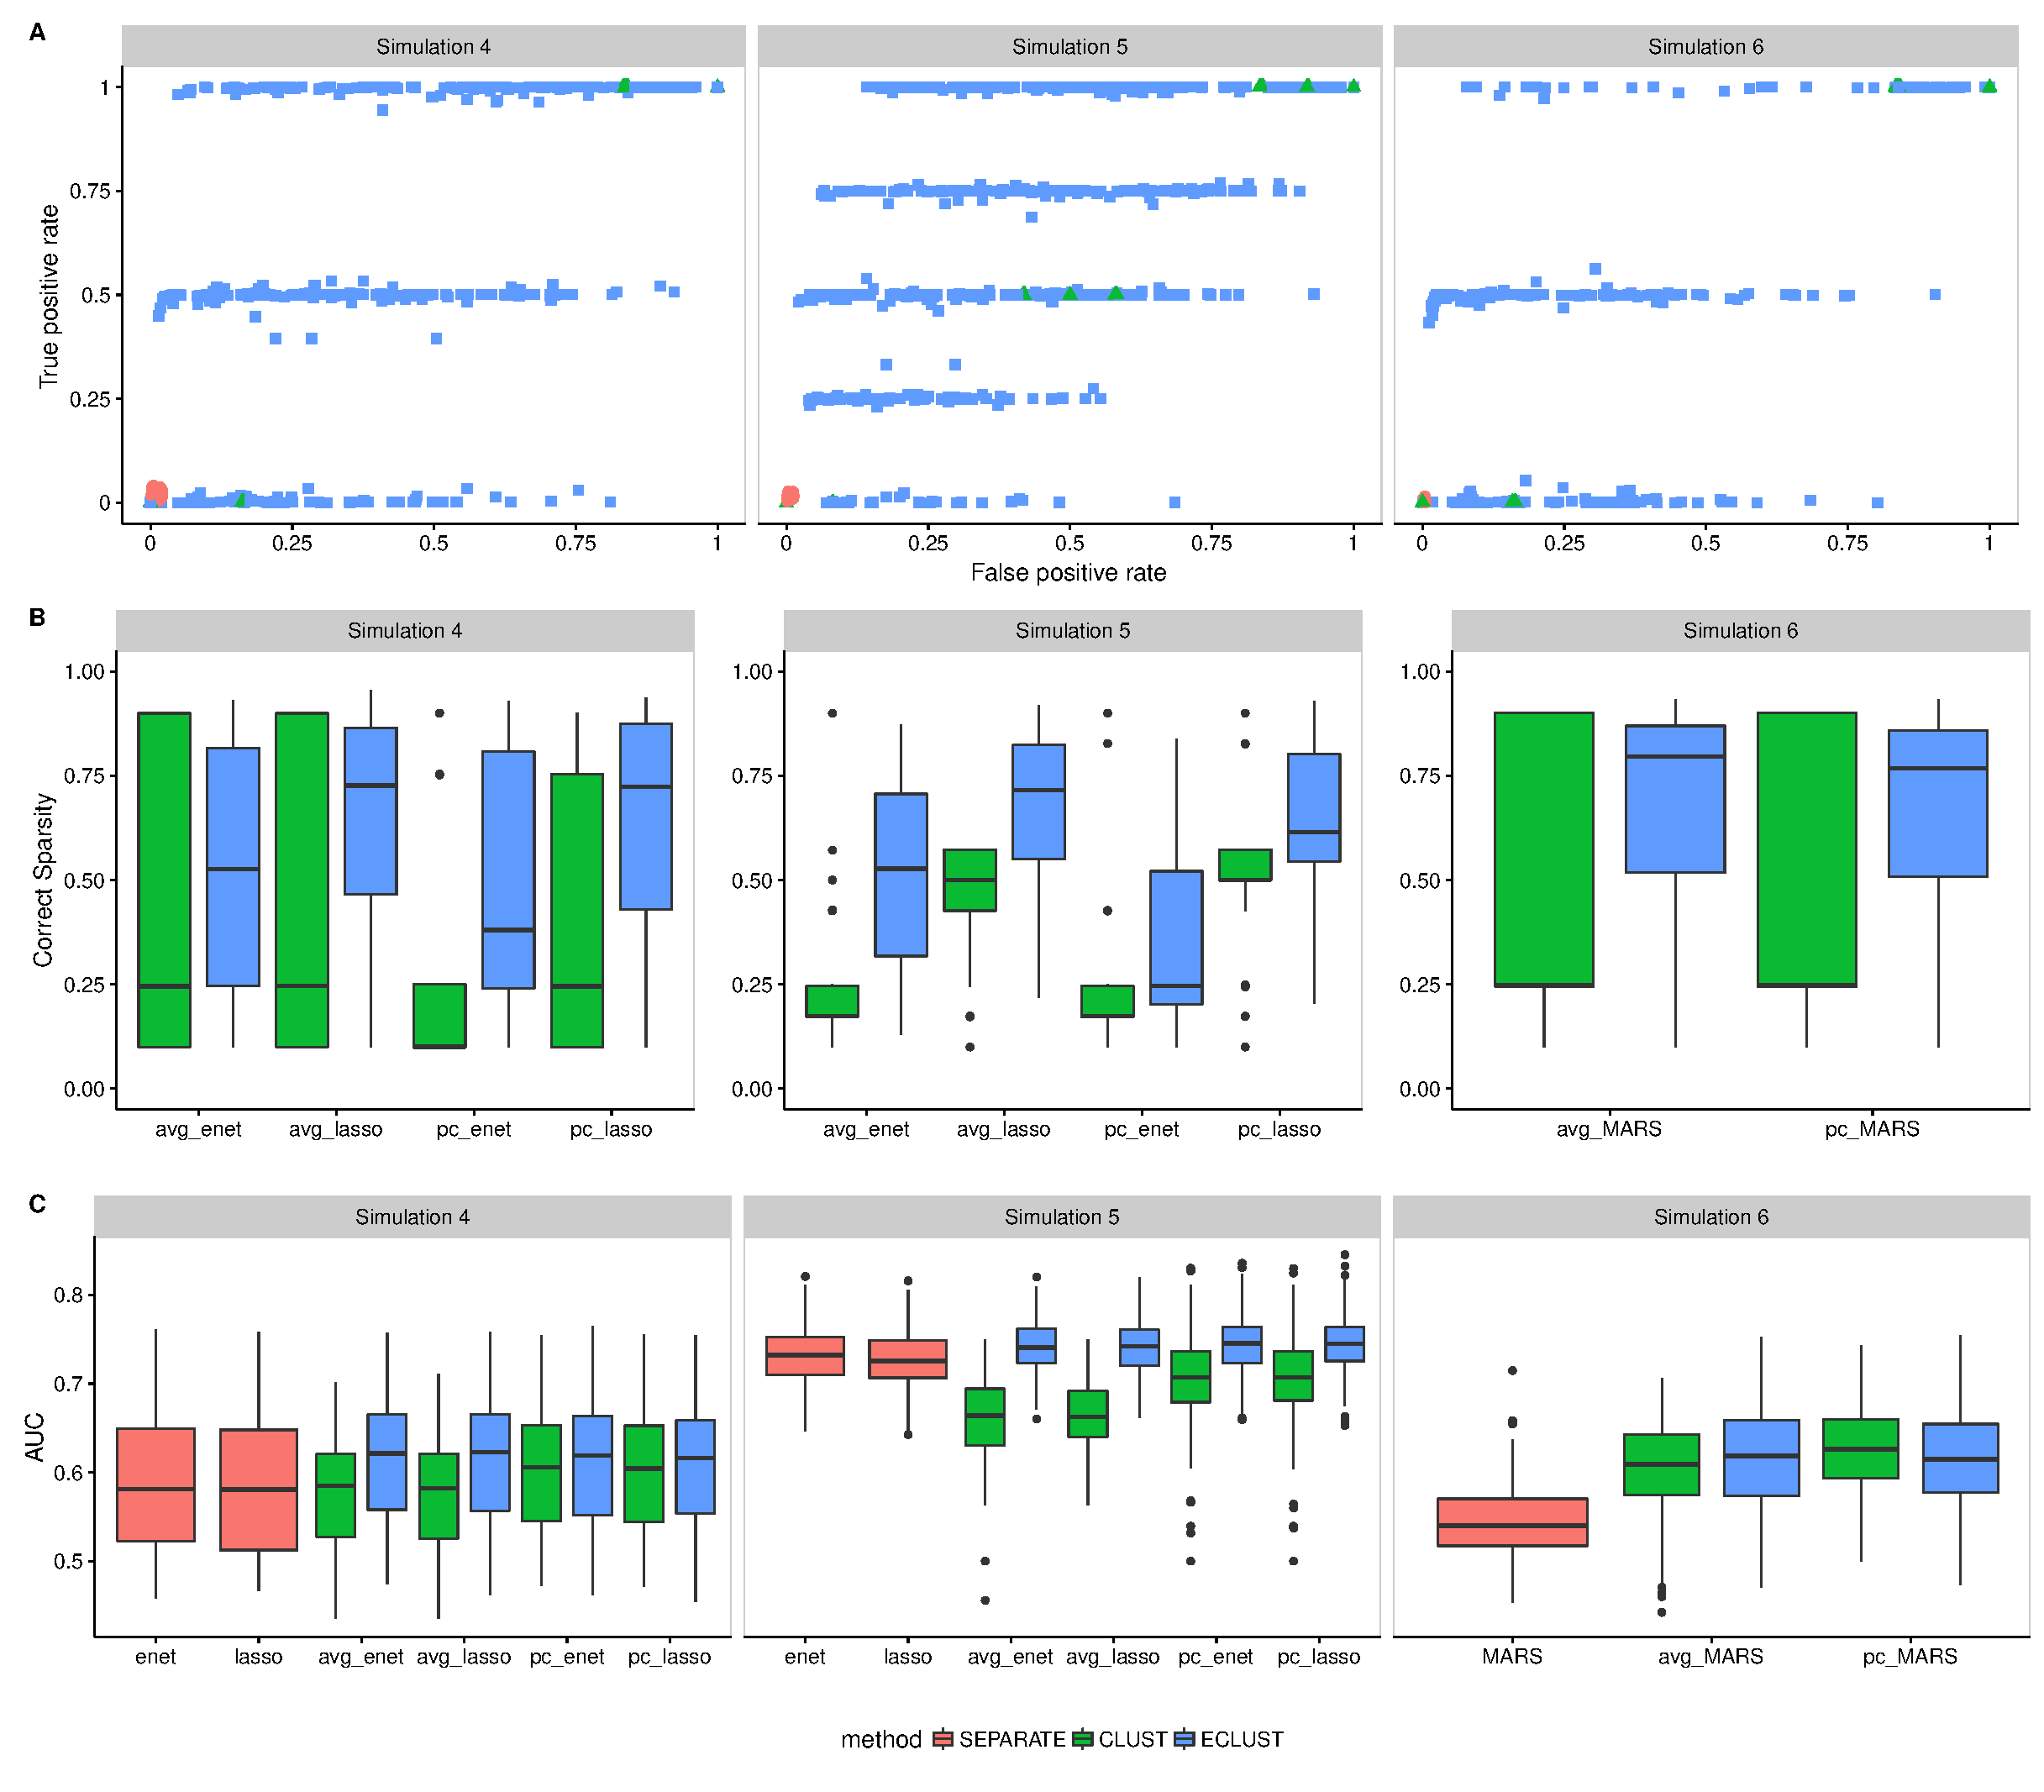
\includegraphics[scale=0.40, keepaspectratio]{./figs/guillimin/results/figures/sim4-5-6-combined/modelfit_sim456.eps}
	%\caption{Model fit results from simulations 4, 5 and 6 for $SNR=1$, $\rho = 0.9$, and \mbox{$\alpha_{j} \sim \tm{Unif}\left[\log(1.9), \log(2.1)\right]$}. SEPARATE results are in pink, CLUST in green and ECLUST in blue.}
	\caption{Model fit results from simulations 4, 5 and 6 for $SNR=1$, $\rho = 0.9$, and \mbox{$\alpha_{j} \sim \tm{Unif}\left[\log(1.9), \log(2.1)\right]$}. SEPARATE results are in pink, CLUST in green and ECLUST in blue.}
	\label{fig:sim-modelfit456}
\end{figure}

\begin{figure}[H]
	\centering
	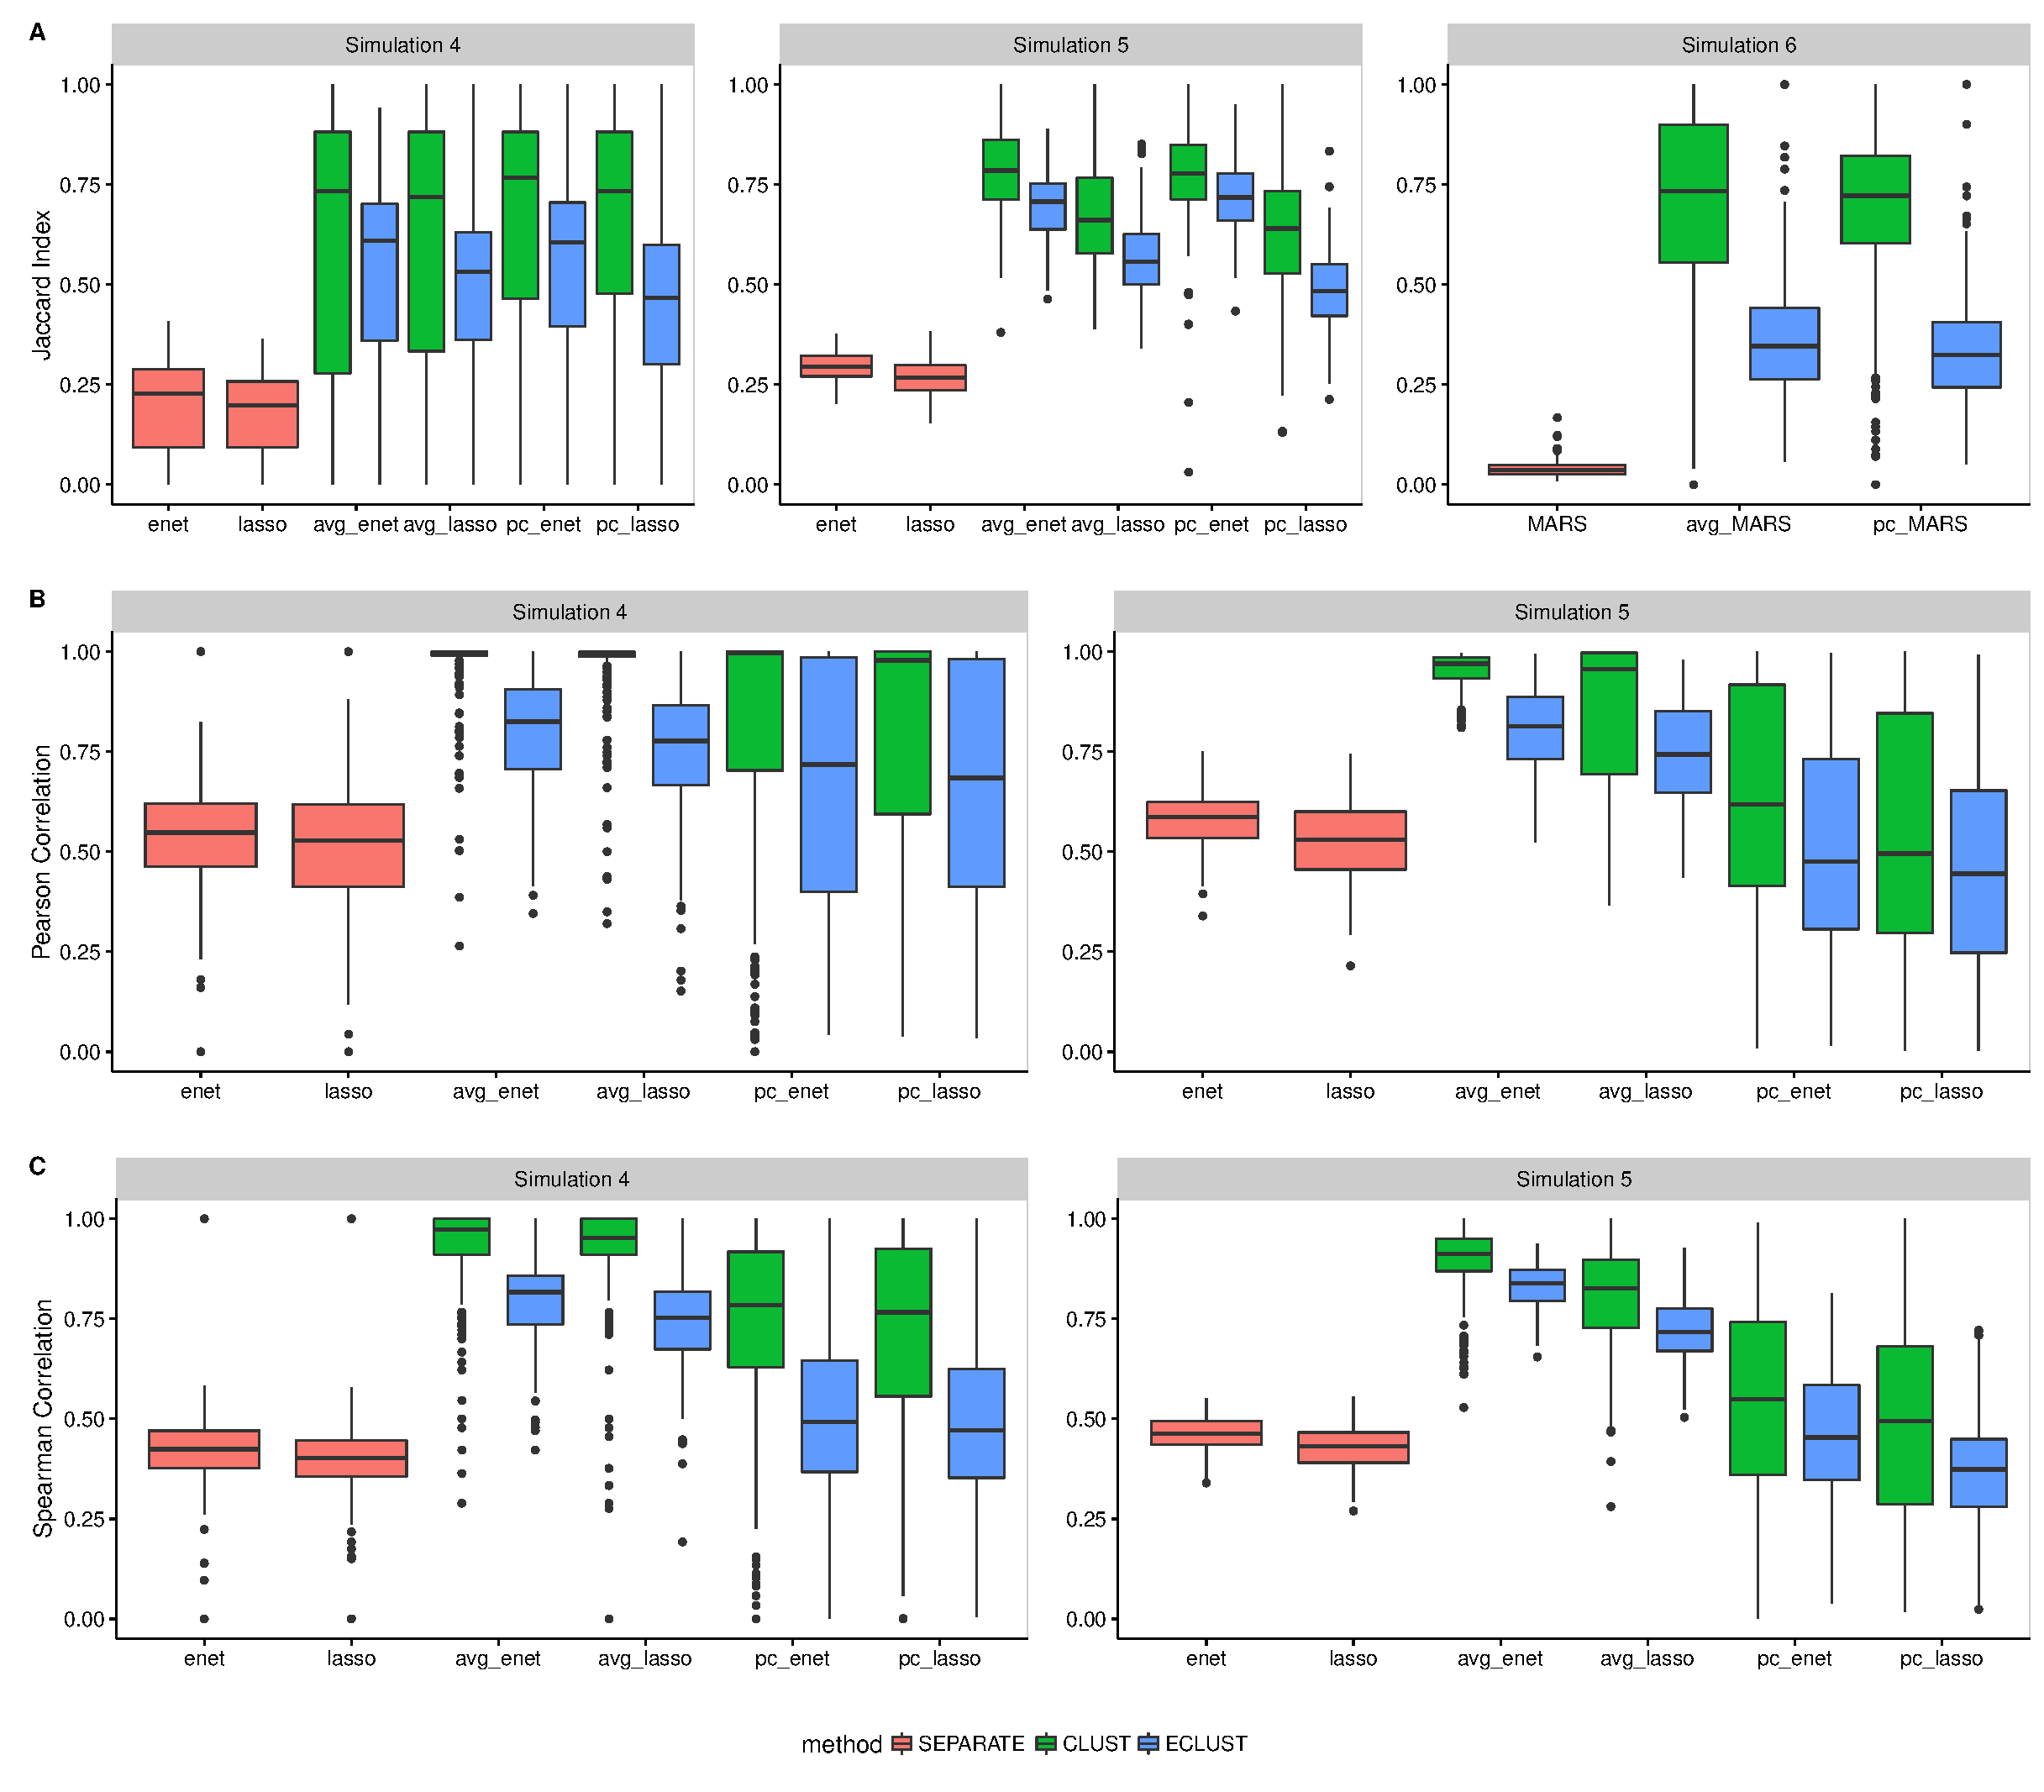
\includegraphics[scale=0.40, keepaspectratio]{./figs/guillimin/results/figures/sim4-5-6-combined/stability_sim456.eps}
	\caption{Stability results from simulations 4, 5 and 6 for $SNR=1$, $\rho = 0.9$, and \mbox{$\alpha_{j} \sim \tm{Unif}\left[\log(1.9), \log(2.1)\right]$}. SEPARATE results are in pink, CLUST in green and ECLUST in blue.}
	\label{fig:sim-stability456}
\end{figure}

\begin{figure}[H]
	\centering
	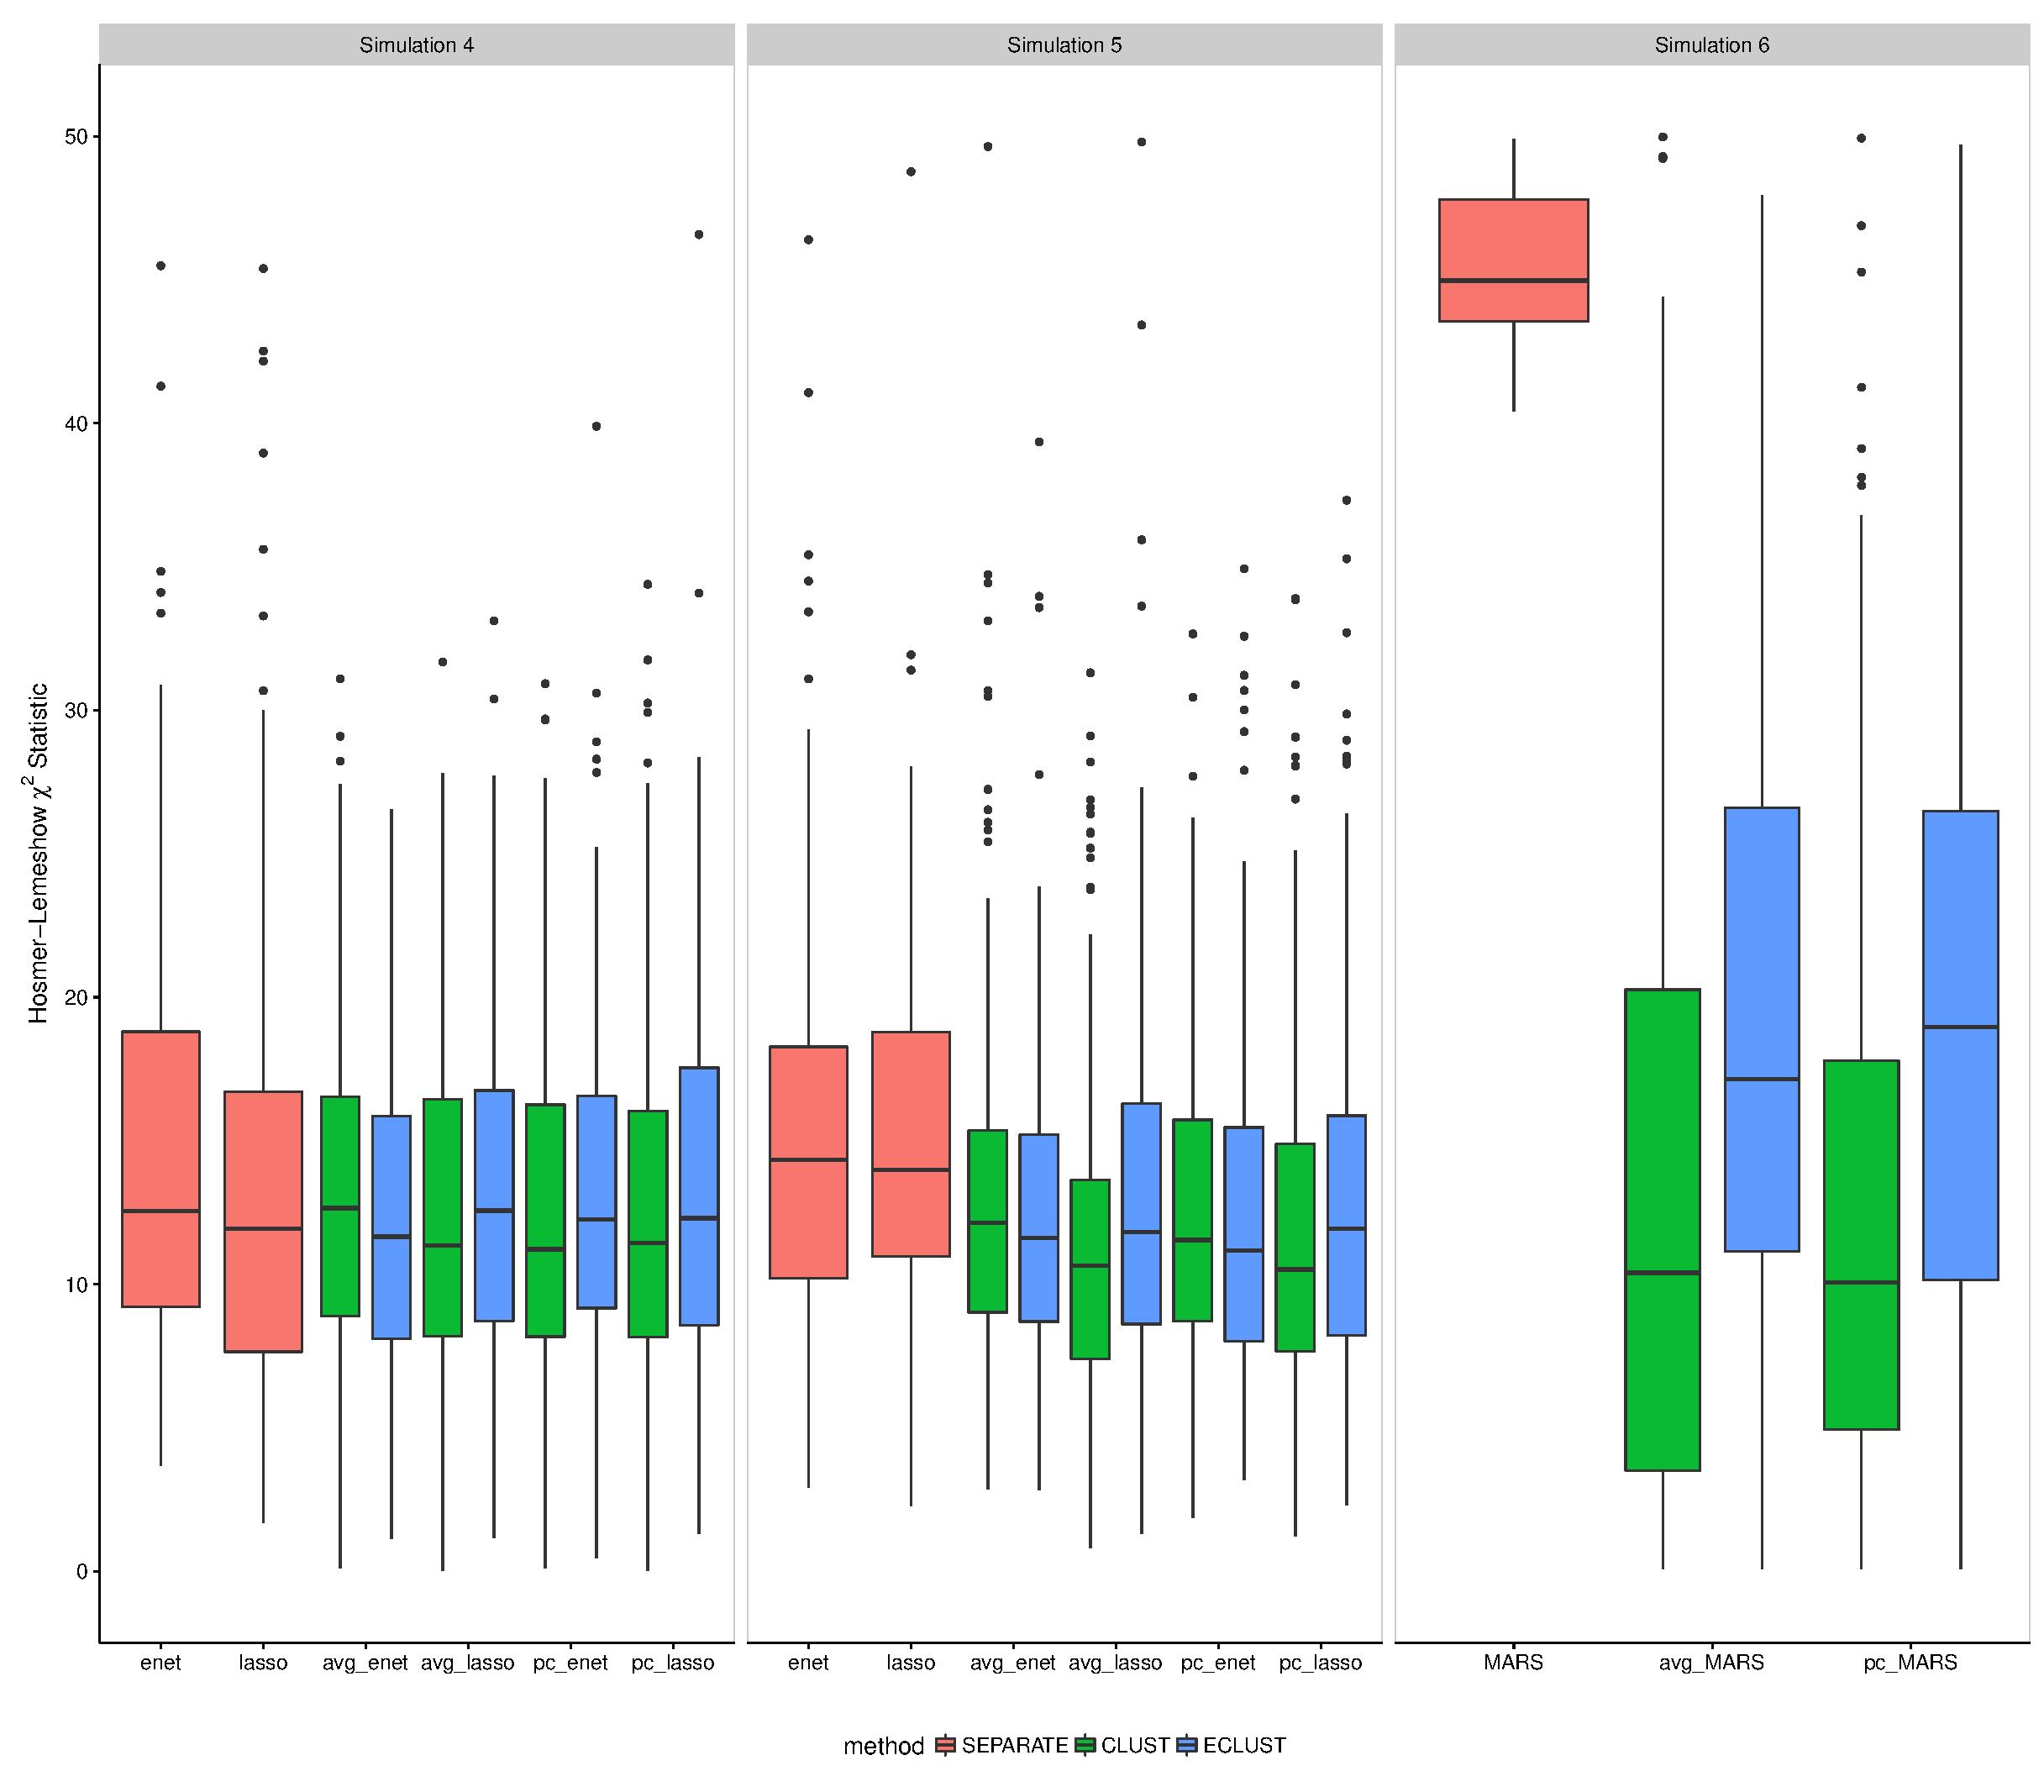
\includegraphics[scale=0.40, keepaspectratio]{./figs/guillimin/results/figures/sim4-5-6-combined/calibration_sim456.eps}
	\caption{Hosmer-Lemeshow statistics from simulations 4, 5 and 6 for $SNR=1$, $\rho = 0.9$, and \mbox{$\alpha_{j} \sim \tm{Unif}\left[\log(1.9), \log(2.1)\right]$}. SEPARATE results are in pink, CLUST in green and ECLUST in blue.}
	\label{fig:sim-calibration456}
\end{figure}


\begin{figure}[H]
	\centering
	\includegraphics[width=1\linewidth]{./figs/guillimin/results/figures/sim4-5-6-combined/calibration-pvalue_sim4.eps}
	\caption{Hosmer-Lemeshow p-values from simulation 4 for $SNR=1$, $\rho = 0.9$, and \mbox{$\alpha_{j} \sim \tm{Unif}\left[\log(1.9), \log(2.1)\right]$}. SEPARATE results are in pink, CLUST in green and ECLUST in blue.}
	\label{fig:sim-calibrationhist4}
\end{figure}


\begin{figure}[H]
	\centering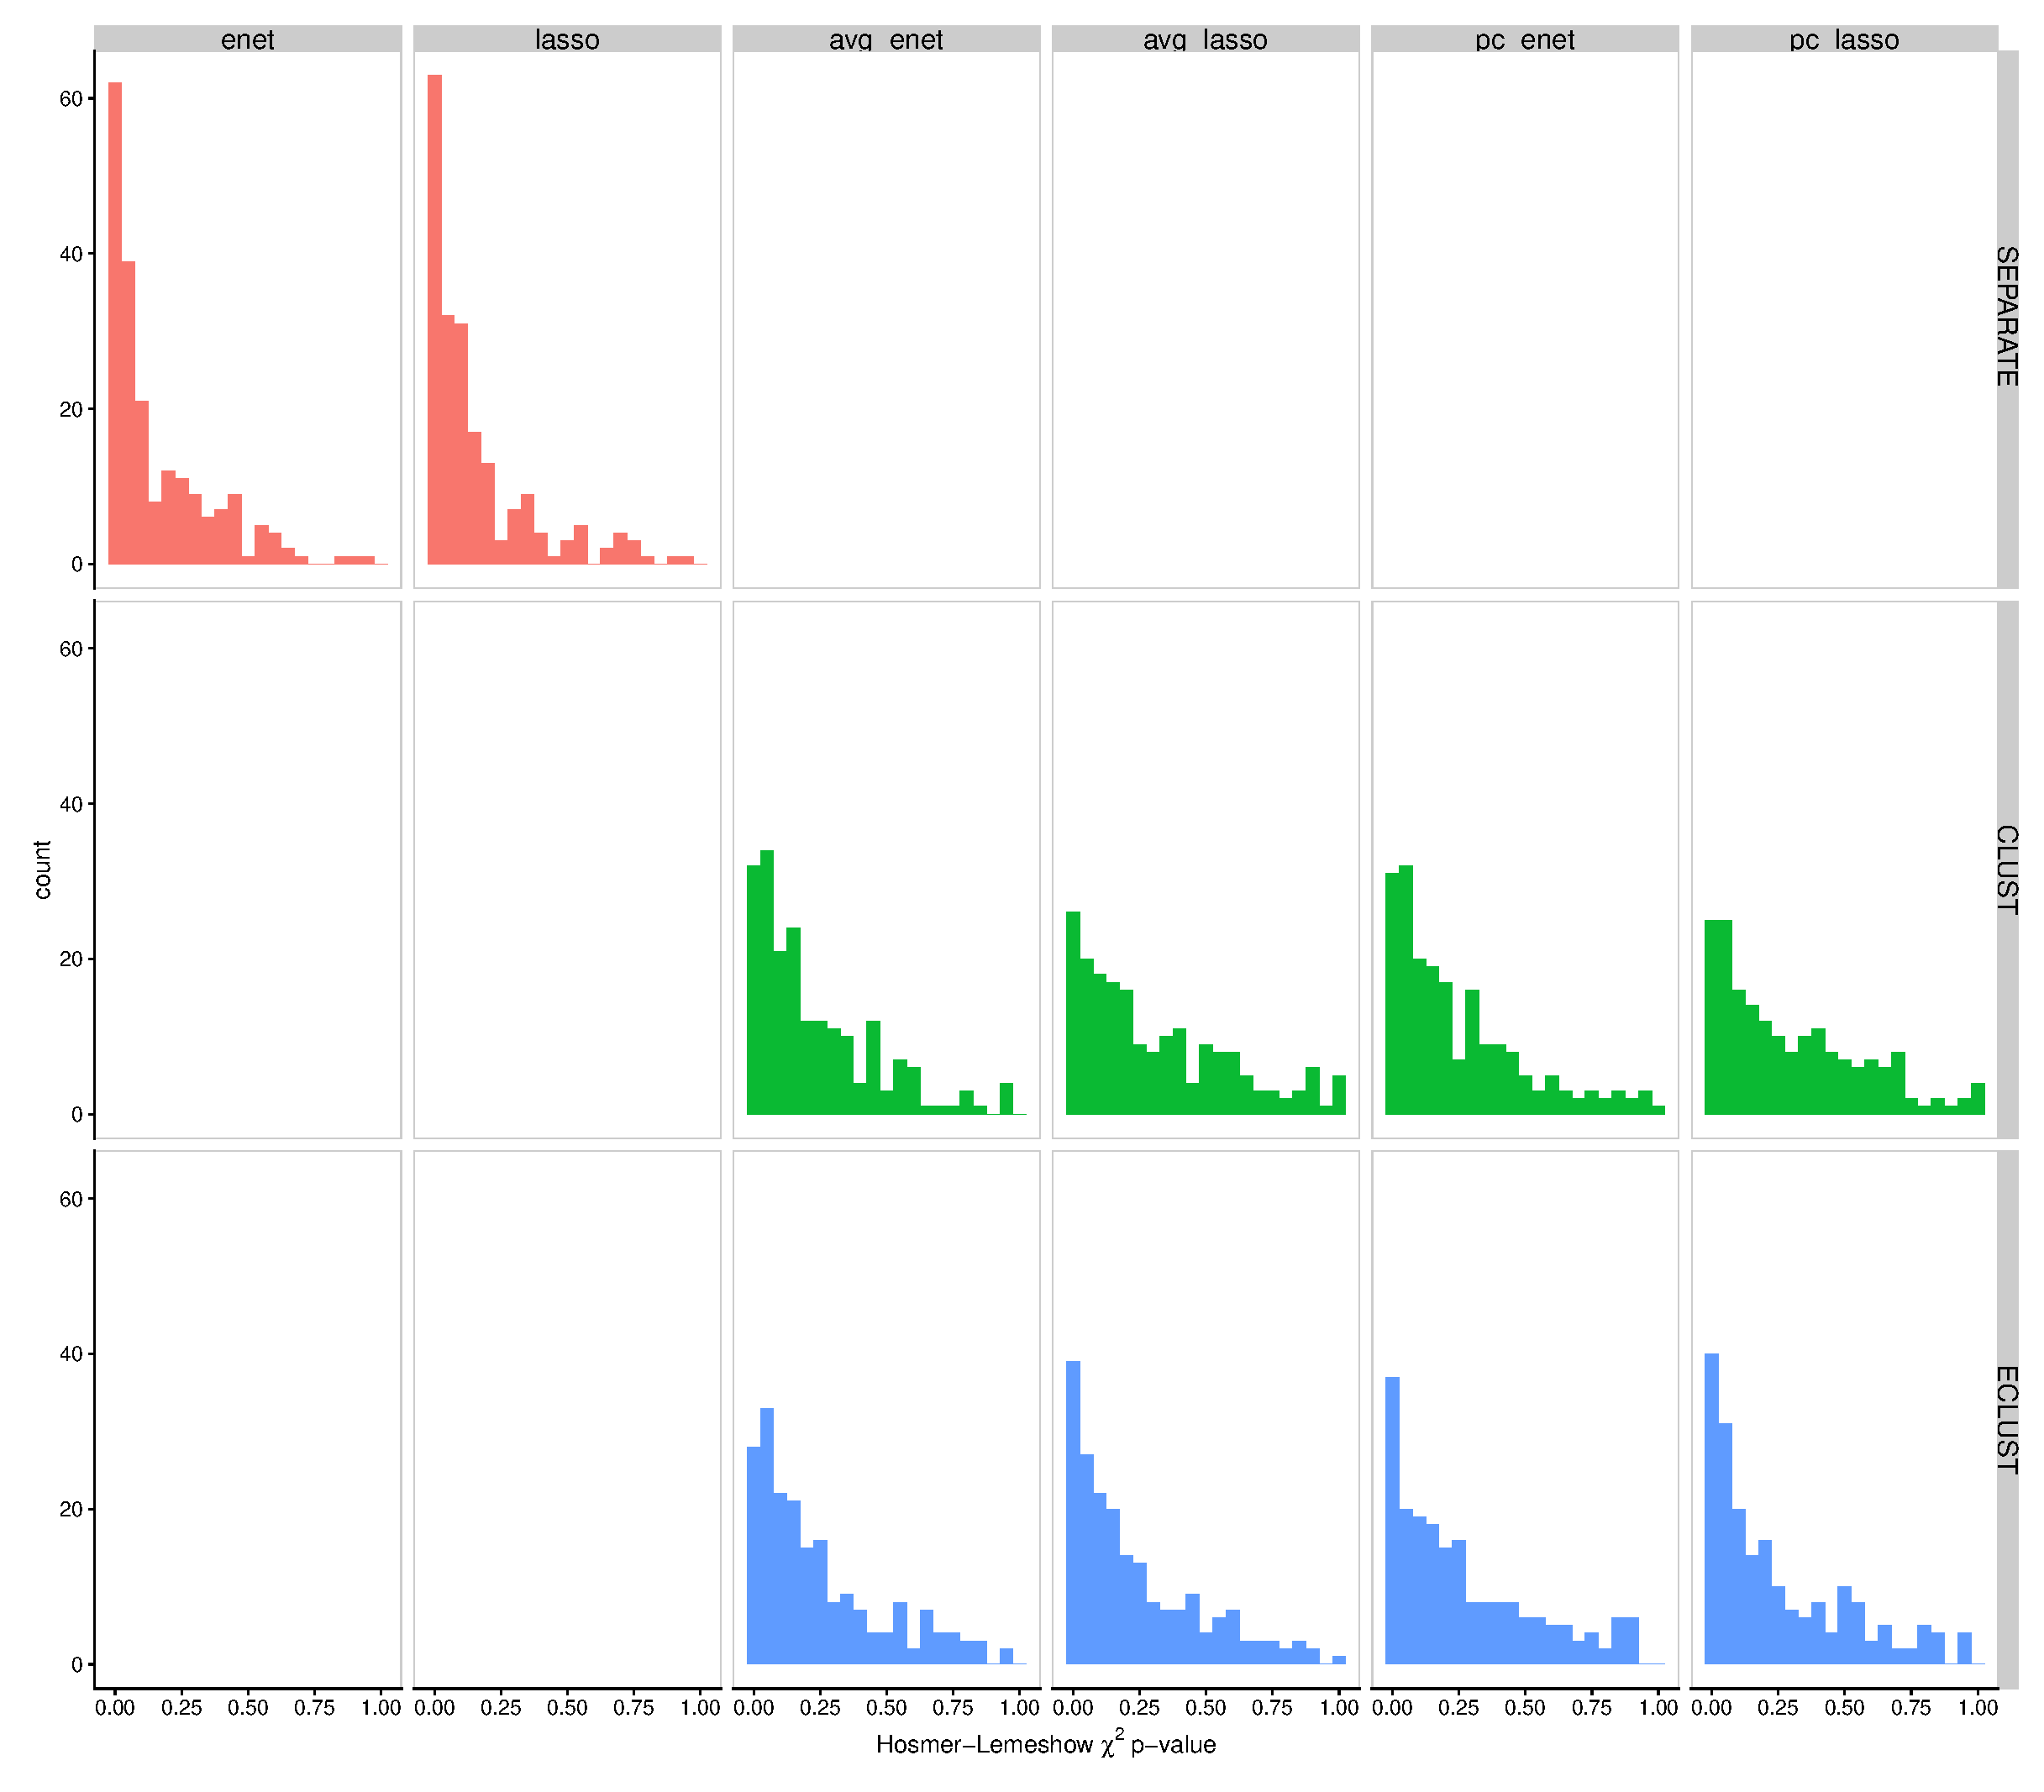
\includegraphics[width=1\linewidth]{./figs/guillimin/results/figures/sim4-5-6-combined/calibration-pvalue_sim5.eps}
	\caption{Hosmer-Lemeshow p-values from simulation 5 for $SNR=1$, $\rho = 0.9$, and \mbox{$\alpha_{j} \sim \tm{Unif}\left[\log(1.9), \log(2.1)\right]$}. SEPARATE results are in pink, CLUST in green and ECLUST in blue.}\label{fig:sim-calibrationhist5}
\end{figure}

\begin{figure}[H]
	\centering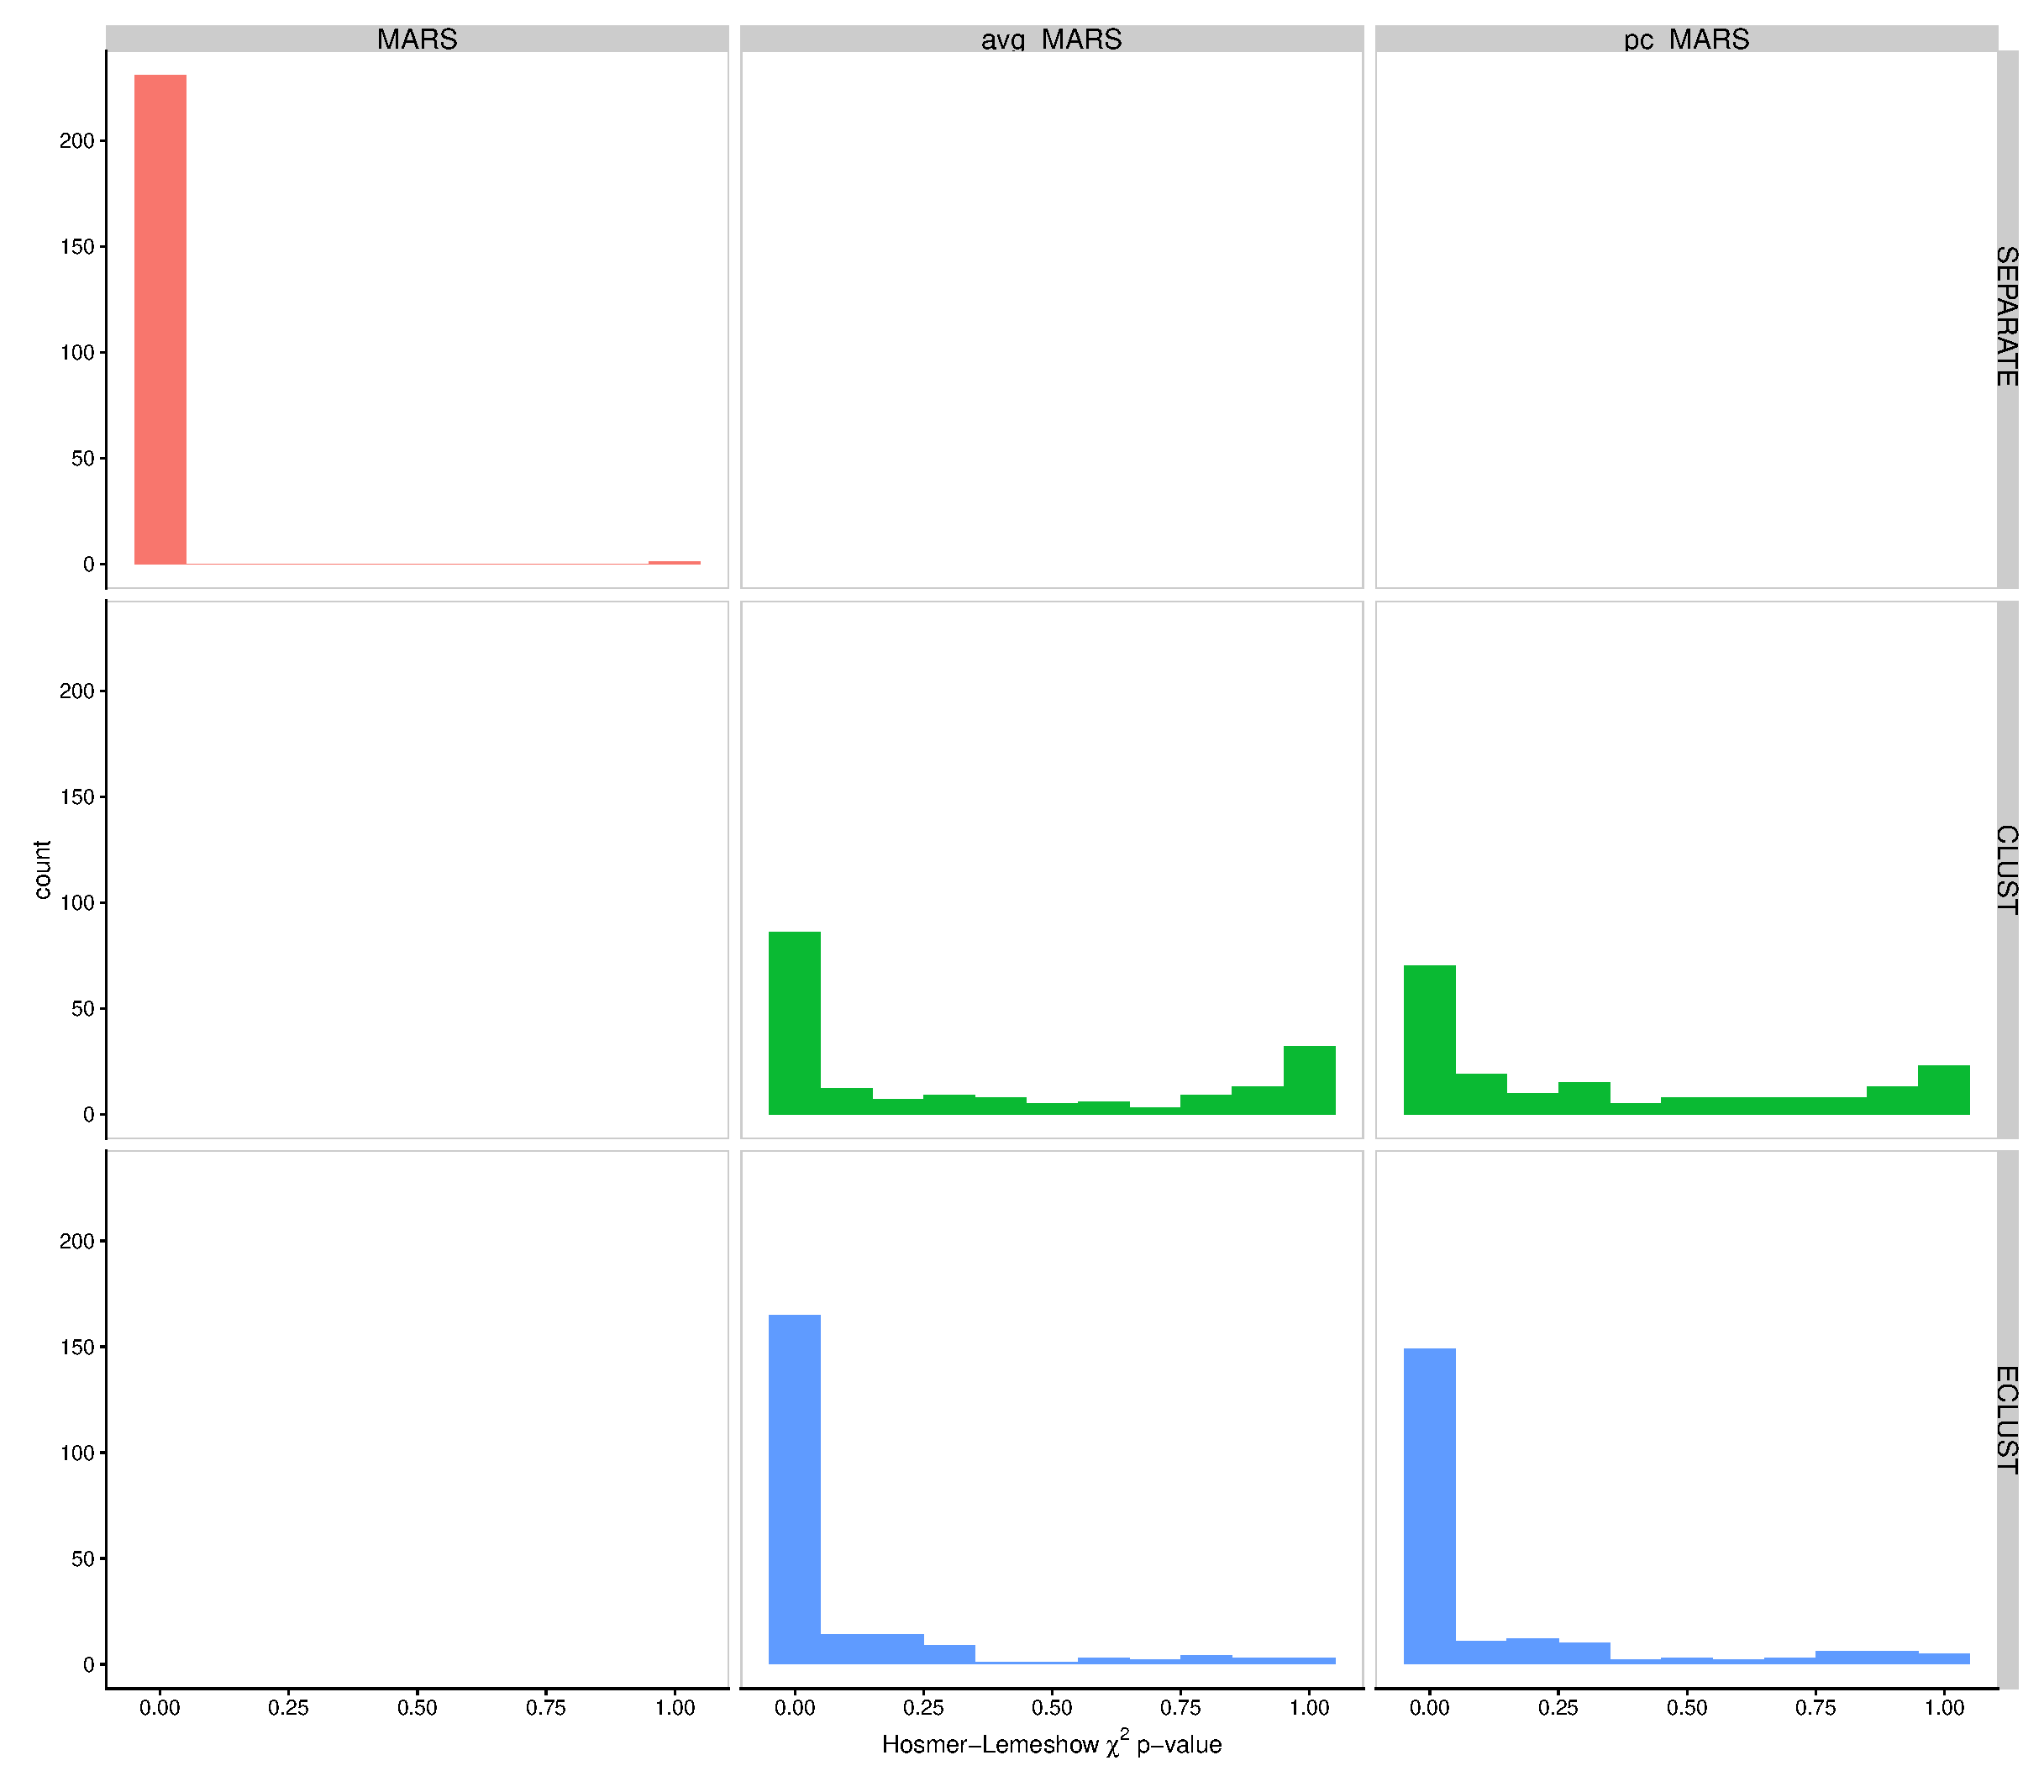
\includegraphics[width=1\linewidth]{./figs/guillimin/results/figures/sim4-5-6-combined/calibration-pvalue_sim6.eps}
	\caption{Hosmer-Lemeshow p-values from simulation 6 for $SNR=1$, $\rho = 0.9$, and \mbox{$\alpha_{j} \sim \tm{Unif}\left[\log(1.9), \log(2.1)\right]$}. SEPARATE results are in pink, CLUST in green and ECLUST in blue.}\label{fig:sim-calibrationhist6}
\end{figure}


\section{Analysis of Clusters}\label{ap:clusters}

\begin{figure}[H]
	\centering
	\includegraphics[scale=0.9, keepaspectratio]{./figs/figures-for-manuscript/nclusters.png}
	\caption{Number of estimated clusters from applying the \texttt{dynamicTreeCut} algorithm to hierarchical clustering of the dissimilarity matrix with average linkage. \mbox{Left panel}: CLUST uses $1-Cor(X_{all})$ and ECLUST uses the euclidean distance of $Cor(X_{\tm{diff}})$ as measures of dissimilarity. Right panel: CLUST uses $1-TOM(X_{all})$ and ECLUST uses the euclidean distance of $TOM(X_{\tm{diff}})$ as measures of dissimilarity. Empirical distributions based on 200 simulation runs.}
	\label{fig:compare_clusters}
\end{figure}


\begin{figure}[H]
	\centering
	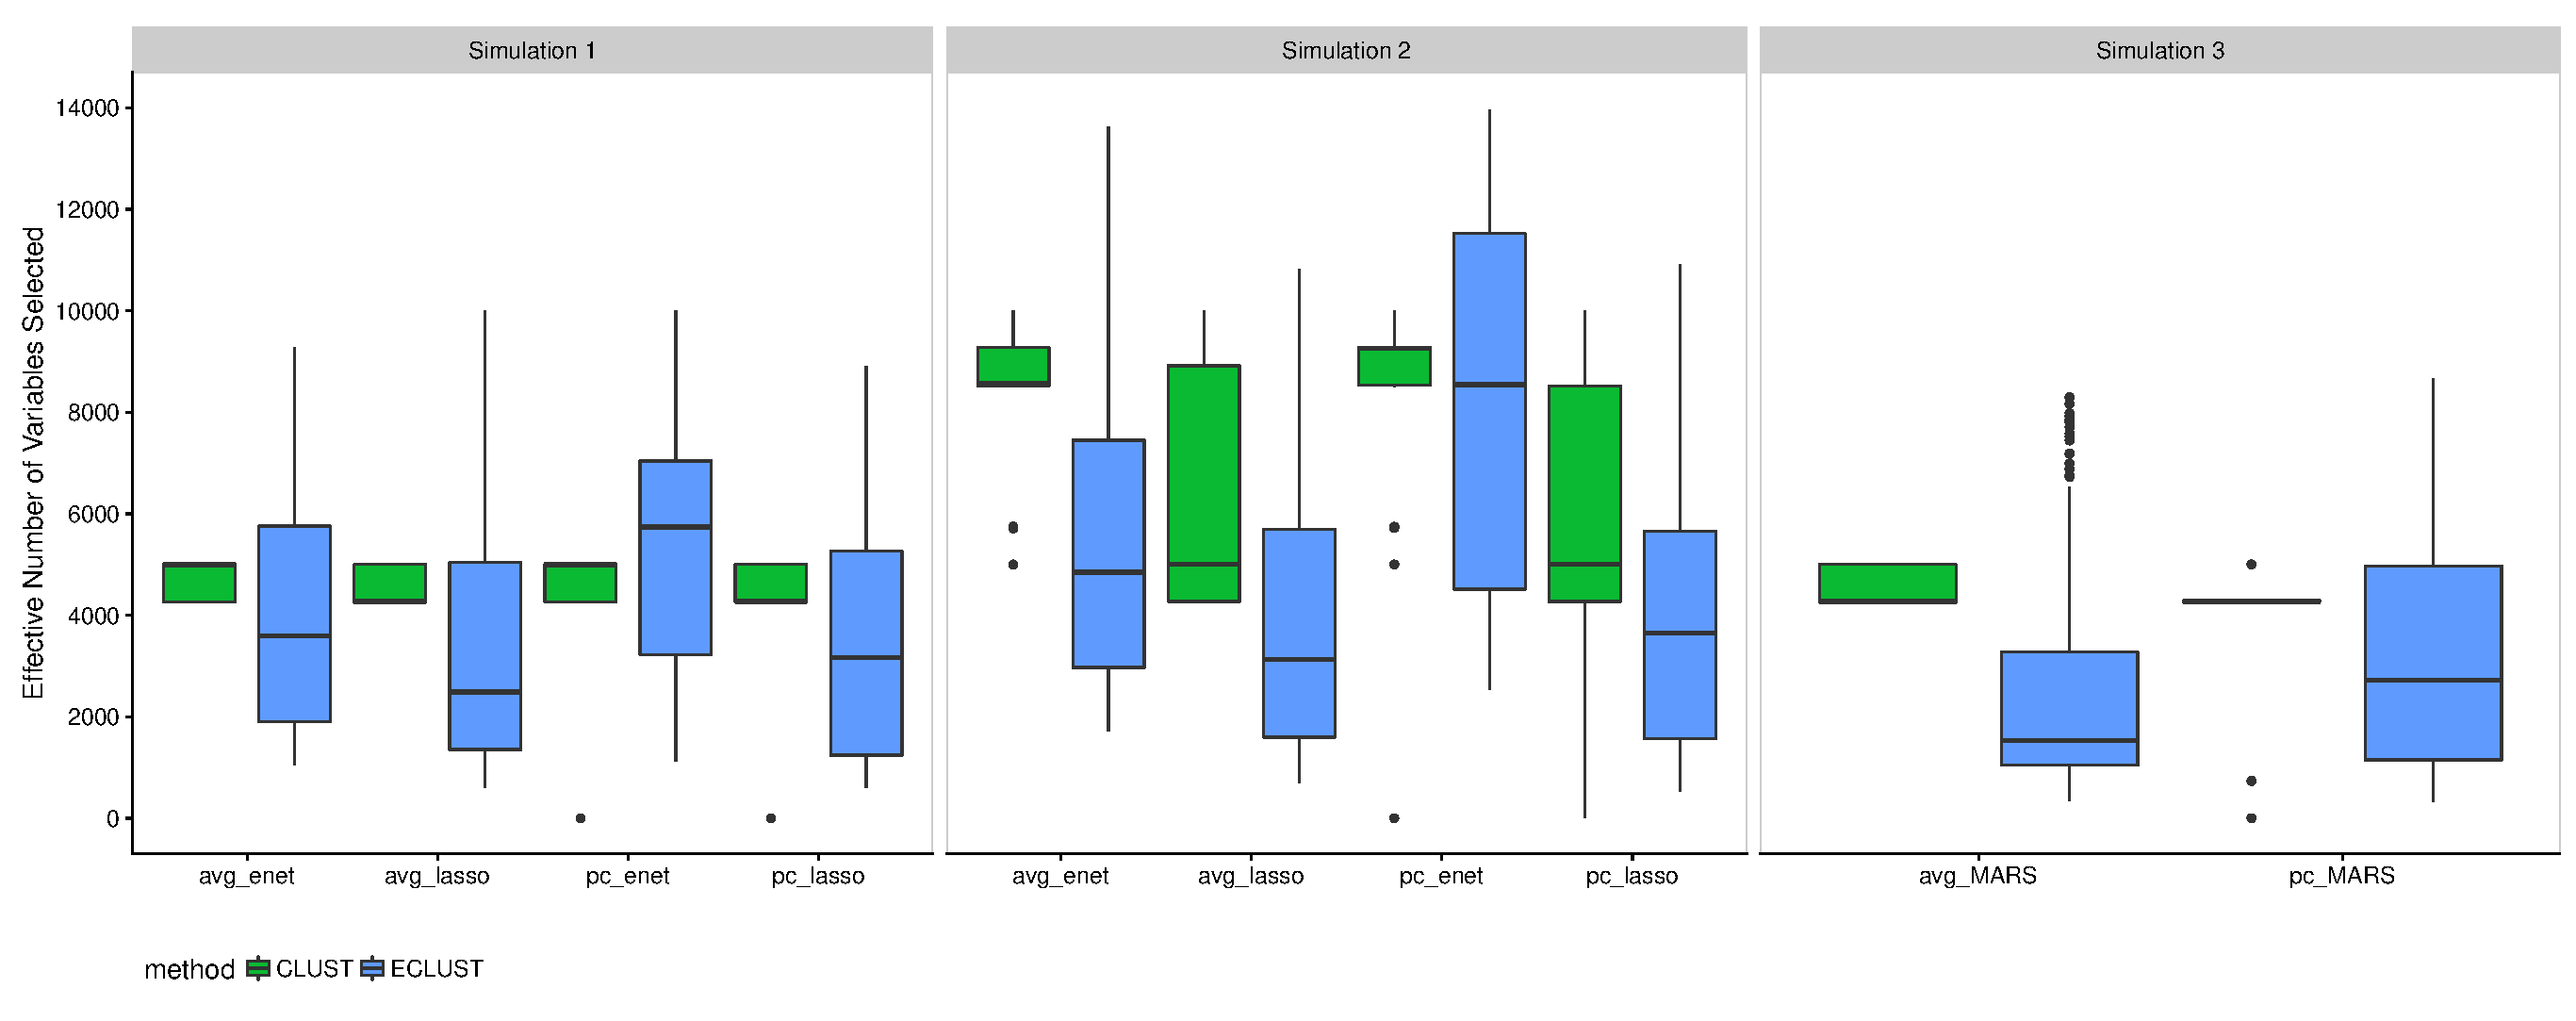
\includegraphics[width=1\linewidth, keepaspectratio]{./figs/guillimin/results/figures/sim4-5-6-combined/Shat_sim123.eps}
	\caption{Effective number of selected variables for simulations 1-3 for $SNR = 1, \rho=0.9$. A variable was considered ``selected'' if its corresponding cluster representative was selected.}
	\label{fig:compare_clusters2}
\end{figure}

\begin{figure}[H]
	\centering
	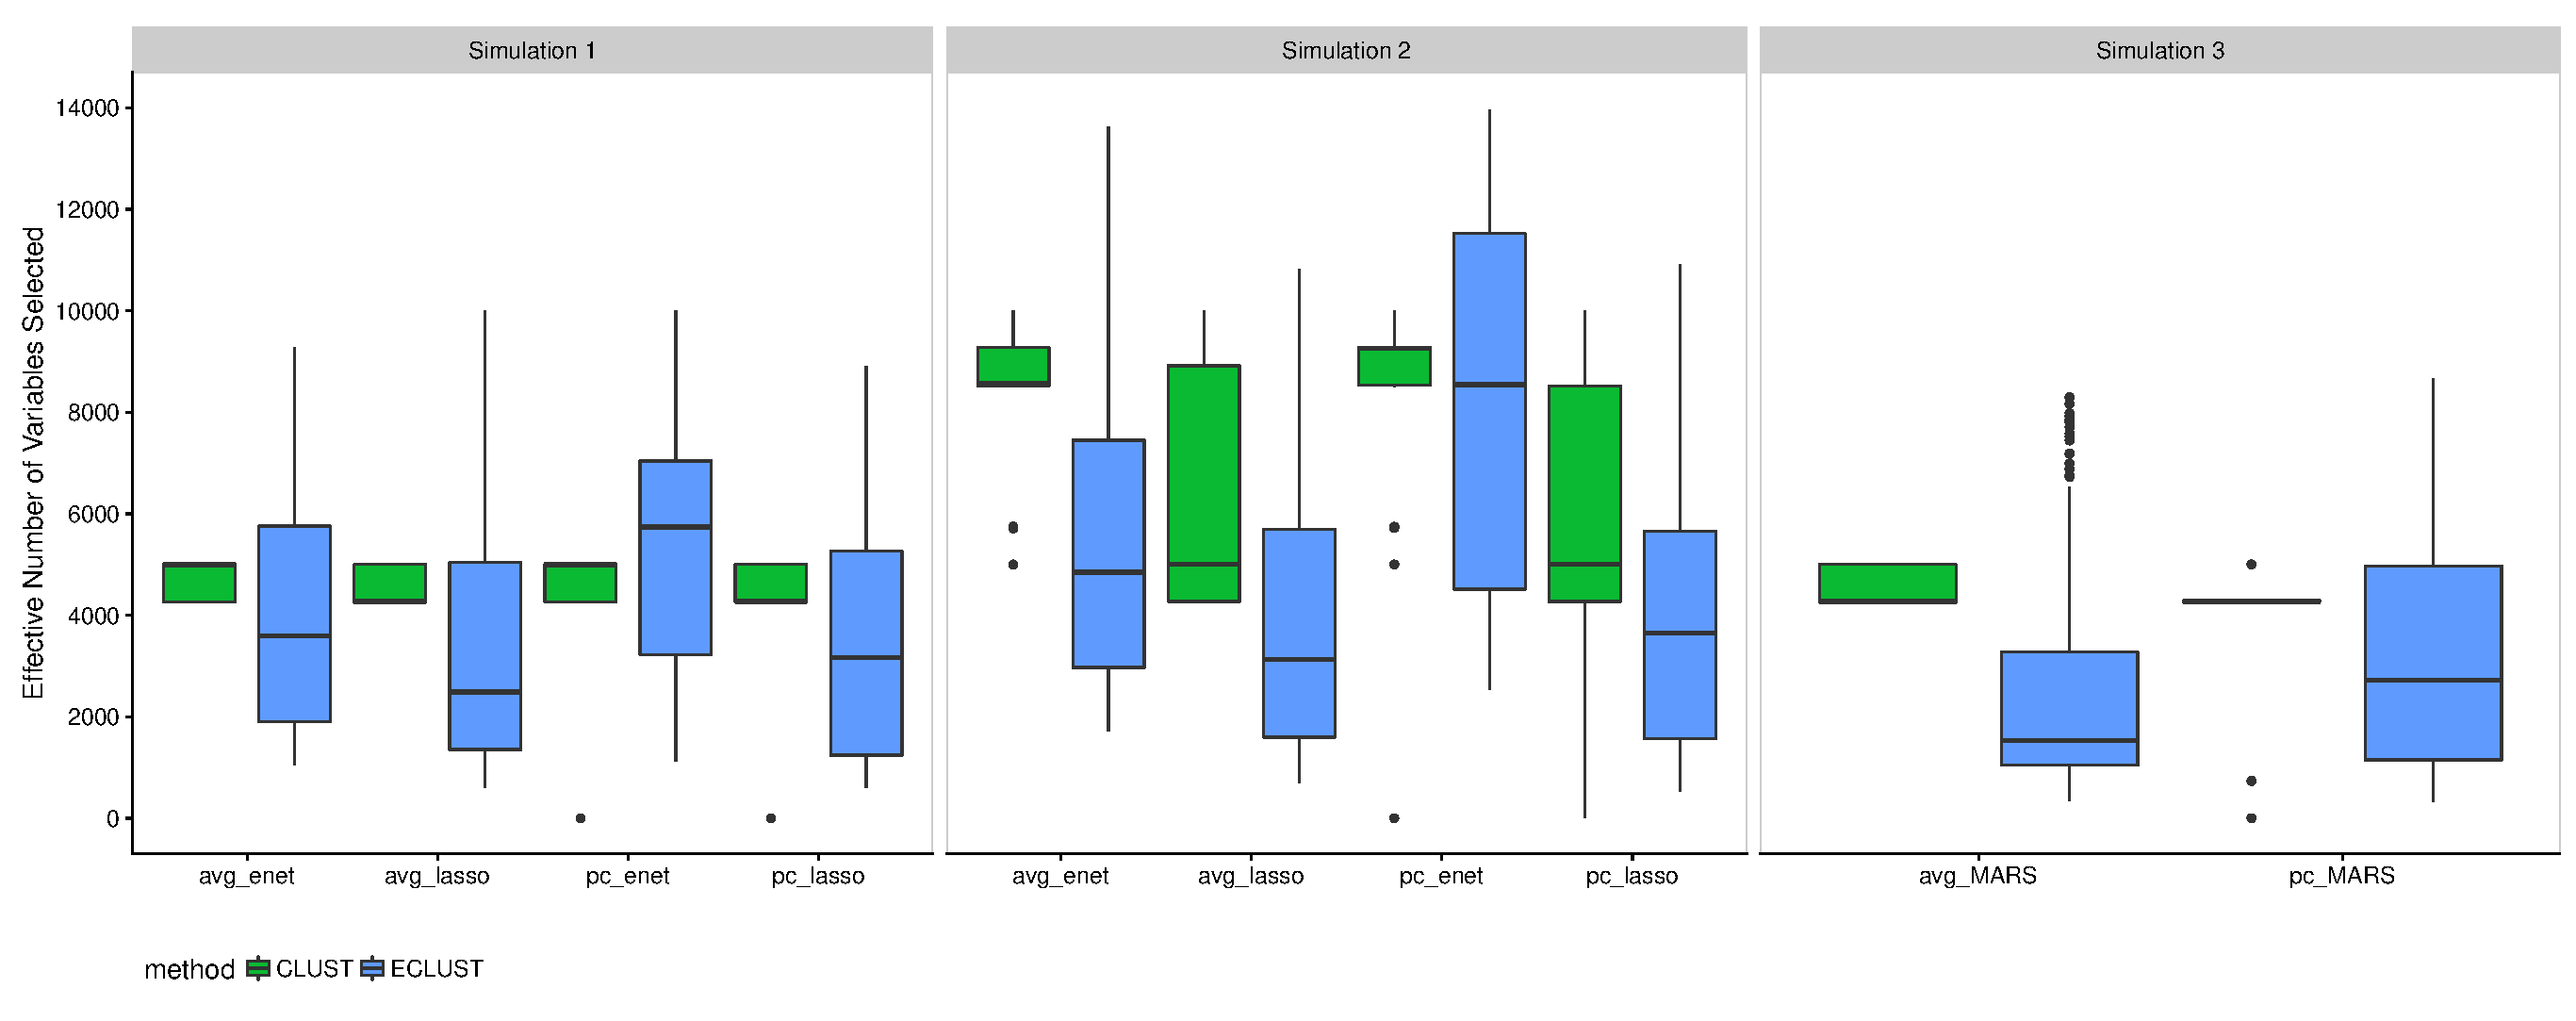
\includegraphics[width=1\linewidth, keepaspectratio]{./figs/guillimin/results/figures/sim4-5-6-combined/Shat_sim123.eps}
	\caption{Effective number of selected variables for simulations 4-6 for $SNR = 1, \rho=0.9$ and \mbox{$\alpha_{j} \sim \tm{Unif}\left[\log(1.9), \log(2.1)\right]$}. A variable was considered ``selected'' if its corresponding cluster representative was selected.}
	\label{fig:compare_clusters3}
\end{figure}


\section{Simulation Results Using TOM as a Measure of Similarity} \label{ap:sim-TOM}


\subsection*{Simulation 1}

\begin{figure}[H]
	\centering
	\includegraphics[scale=0.6, keepaspectratio]{./figs/hydra/results/figures/sim1-sept10/RMSE_TOM_sim1.png}
	\caption{Simulation 1 -- Root mean squared error on an independent test set using the TOM as a measure of similarity from 200 simulation runs. Vertical panels represent varying correlation between active clusters. Horizontal panels represent different signal-to-noise ratios.}
	\label{fig:RMSE_TOM_sim1}
\end{figure}

\begin{figure}[H]
	\centering
	\includegraphics[scale=0.6, keepaspectratio]{./figs/hydra/results/figures/sim1-sept10/CorrectSparsity_TOM_sim1.png}
	\caption{Simulation 1 -- Correct Sparsity based on the training set using the TOM as a measure of similarity from 200 simulation runs. Vertical panels represent varying correlation between active clusters. Horizontal panels represent different signal-to-noise ratios.}
	\label{fig:CorrectSparsity_TOM_sim1}
\end{figure}


\begin{figure}
	\includegraphics[scale=0.6, keepaspectratio]{./figs/hydra/results/figures/sim1-sept10/tpr_fpr_TOM_sim1.png}
	\caption{Simulation 1 -- True positive rate vs. false positive rate based on the training set using the TOM as a measure of similarity. Each point represents 1 simulation run (there are a total of 200 simulation runs). Vertical panels represent varying correlation between active clusters. Horizontal panels represent different signal-to-noise ratios.}
	\label{fig:tpr_fpr_TOM_sim1}
\end{figure}


\begin{figure}[H]
	\centering
	\includegraphics[scale=0.6, keepaspectratio]{./figs/hydra/results/figures/sim1-sept10/jacc_TOM_sim1.png}
	\caption{Simulation 1 -- Average Jaccard Index from 10 CV folds of the training set using the TOM as a measure of similarity. We fit the model to each of the 10 CV folds resulting in 10 sets of selected predictors. We then calculate the Jaccard Index between all $\binom{10}{2}$ possible combinations of these sets and take the average. This process is repeated for each of the 200 simulation runs. Vertical panels represent varying correlation between active clusters. Horizontal panels represent different signal-to-noise ratios.}
	\label{fig:jacc_TOM_sim1}
\end{figure}


\begin{figure}[H]
	\centering
	\includegraphics[scale=0.6, keepaspectratio]{./figs/hydra/results/figures/sim1-sept10/spearman_TOM_sim1.png}
	\caption{Simulation 1 -- Average Spearman correlation from 10 CV folds of the training set using the TOM as a measure of similarity. We fit the model to each of the 10 CV folds resulting in 10 sets of estimated regression coefficients. We then calculate the Spearman correlation between all $\binom{10}{2}$ possible combinations of these sets and take the average. This process is repeated for each of the 200 simulation runs. Vertical panels represent varying correlation between active clusters. Horizontal panels represent different signal-to-noise ratios.}
	\label{fig:spearman_TOM_sim1}
\end{figure}


\begin{figure}[H]
	\centering
	\includegraphics[scale=0.6, keepaspectratio]{./figs/hydra/results/figures/sim1-sept10/pearson_TOM_sim1.png}
	\caption{Simulation 1 -- Average Pearson correlation from 10 CV folds of the training set using the TOM as a measure of similarity. We fit the model to each of the 10 CV folds resulting in 10 sets of estimated regression coefficients. We then calculate the Pearson correlation between all $\binom{10}{2}$ possible combinations of these sets and take the average. This process is repeated for each of the 200 simulation runs. Vertical panels represent varying correlation between active clusters. Horizontal panels represent different signal-to-noise ratios.}
	\label{fig:pearson_TOM_sim1}
\end{figure}

\subsection*{Simulation 2}
\begin{figure}[H]
	\centering
	\includegraphics[scale=0.55, keepaspectratio]{./figs/hydra/results/figures/sim2-sept8/RMSE_TOM_sim2.png}
	\caption{Simulation 2 -- Root mean squared error on an independent test set using the TOM as a measure of similarity from 200 simulation runs. \mbox{(A) $\alpha_{j} \sim \tm{Unif}\left[0.4, 0.6\right]$}, \mbox{(B) $\alpha_{j} \sim \tm{Unif}\left[1.9, 2.1\right]$}. Vertical panels represent varying correlation between active clusters. Horizontal panels represent different signal-to-noise ratios.}
	\label{fig:RMSE_TOM_sim2}
\end{figure}

\begin{figure}[H]
	\centering
	\includegraphics[scale=0.58, keepaspectratio]{./figs/hydra/results/figures/sim2-sept8/CorrectSparsity_TOM_sim2.png}
	\caption{Simulation 2 -- Correct Sparsity based on the training set using the TOM as a measure of similarity from 200 simulation runs. \mbox{(A) $\alpha_{j} \sim \tm{Unif}\left[0.4, 0.6\right]$}, \mbox{(B) $\alpha_{j} \sim \tm{Unif}\left[1.9, 2.1\right]$}. Vertical panels represent varying correlation between active clusters. Horizontal panels represent different signal-to-noise ratios.}
	\label{fig:CorrectSparsity_TOM_sim2}
\end{figure}


\begin{figure}
	\includegraphics[scale=0.57, keepaspectratio]{./figs/hydra/results/figures/sim2-sept8/tpr_fpr_TOM_sim2.png}
	\caption{Simulation 2 -- True positive rate vs. false positive rate based on the training set using the TOM as a measure of similarity. \mbox{(A) $\alpha_{j} \sim \tm{Unif}\left[0.4, 0.6\right]$}, \mbox{(B) $\alpha_{j} \sim \tm{Unif}\left[1.9, 2.1\right]$}. Each point represents 1 simulation run (there are a total of 200 simulation runs). Vertical panels represent varying correlation between active clusters. Horizontal panels represent different signal-to-noise ratios.}
	\label{fig:tpr_fpr_TOM_sim2}
\end{figure}

%\begin{sidewaysfigure}
%	\includegraphics[width=0.9\columnwidth]{./hydra/results/figures/sim2-sept8/tpr_fpr_alpha2sim2.png}
%	\caption{True positive rate vs. false positive rate for $\alpha_{jE} \sim \tm{Unif}\left[1.9, 2.1\right]$}
%	\label{fig:sim2-corvstom2}
%\end{sidewaysfigure}


\begin{figure}[H]
	\centering
	\includegraphics[scale=0.55, keepaspectratio]{./figs/hydra/results/figures/sim2-sept8/jacc_TOM_sim2.png}
	\caption{Simulation 2 -- Average Jaccard Index from 10 CV folds of the training set using the TOM as a measure of similarity. \mbox{(A) $\alpha_{j} \sim \tm{Unif}\left[0.4, 0.6\right]$}, \mbox{(B) $\alpha_{j} \sim \tm{Unif}\left[1.9, 2.1\right]$}. We fit the model to each of the 10 CV folds resulting in 10 sets of selected predictors. We then calculate the Jaccard Index between all $\binom{10}{2}$ possible combinations of these sets and take the average. This process is repeated for each of the 200 simulation runs. Vertical panels represent varying correlation between active clusters. Horizontal panels represent different signal-to-noise ratios.}
	\label{fig:jacc_TOM_sim2}
\end{figure}


\begin{figure}[H]
	\centering
	\includegraphics[scale=0.52, keepaspectratio]{./figs/hydra/results/figures/sim2-sept8/spearman_TOM_sim2.png}
	\caption{Simulation 2 -- Average Spearman correlation from 10 CV folds of the training set using the TOM as a measure of similarity. \mbox{(A) $\alpha_{j} \sim \tm{Unif}\left[0.4, 0.6\right]$}, \mbox{(B) $\alpha_{j} \sim \tm{Unif}\left[1.9, 2.1\right]$}. We fit the model to each of the 10 CV folds resulting in 10 sets of estimated regression coefficients. We then calculate the Spearman correlation between all $\binom{10}{2}$ possible combinations of these sets and take the average. This process is repeated for each of the 200 simulation runs. Vertical panels represent varying correlation between active clusters. Horizontal panels represent different signal-to-noise ratios.}
	\label{fig:spearman_TOM_sim2}
\end{figure}

\begin{figure}[H]
	\centering
	\includegraphics[scale=0.55, keepaspectratio]{./figs/hydra/results/figures/sim2-sept8/pearson_TOM_sim2.png}
	\caption{Simulation 2 -- Average Pearson correlation from 10 CV folds of the training set using the TOM as a measure of similarity. \mbox{(A) $\alpha_{j} \sim \tm{Unif}\left[0.4, 0.6\right]$}, \mbox{(B) $\alpha_{j} \sim \tm{Unif}\left[1.9, 2.1\right]$}. We fit the model to each of the 10 CV folds resulting in 10 sets of estimated regression coefficients. We then calculate the Pearson correlation between all $\binom{10}{2}$ possible combinations of these sets and take the average. This process is repeated for each of the 200 simulation runs. Vertical panels represent varying correlation between active clusters. Horizontal panels represent different signal-to-noise ratios.}
	\label{fig:pearson_TOM_sim2}
\end{figure}




\subsection*{Simulation 3}

\begin{figure}[H]
	\centering
	\includegraphics[scale=0.6, keepaspectratio]{./figs/hydra/results/figures/sim3-sept27/RMSE_TOM_sim3.png}
	\caption{Simulation 3 -- Root mean squared error on an independent test set using the TOM as a measure of similarity from 200 simulation runs. Vertical panels represent varying correlation between active clusters. Horizontal panels represent different signal-to-noise ratios.}
	\label{fig:RMSE_TOM_sim3}
\end{figure}

\begin{figure}[H]
	\centering
	\includegraphics[scale=0.6, keepaspectratio]{./figs/hydra/results/figures/sim3-sept27/CorrectSparsity_TOM_sim3.png}
	\caption{Simulation 3 -- Correct Sparsity based on the training set using the TOM as a measure of similarity from 200 simulation runs. Vertical panels represent varying correlation between active clusters. Horizontal panels represent different signal-to-noise ratios.}
	\label{fig:CorrectSparsity_TOM_sim3}
\end{figure}


\begin{figure}
	\includegraphics[scale=0.6, keepaspectratio]{./figs/hydra/results/figures/sim3-sept27/tpr_fpr_TOM_sim3.png}
	\caption{Simulation 3 -- True positive rate vs. false positive rate based on the training set using the TOM as a measure of similarity. Each point represents 1 simulation run (there are a total of 200 simulation runs). Vertical panels represent varying correlation between active clusters. Horizontal panels represent different signal-to-noise ratios.}
	\label{fig:tpr_fpr_TOM_sim3}
\end{figure}


\begin{figure}[H]
	\centering
	\includegraphics[scale=0.6, keepaspectratio]{./figs/hydra/results/figures/sim3-sept27/jacc_TOM_sim3.png}
	\caption{Simulation 3 -- Average Jaccard Index from 10 CV folds of the training set using the TOM as a measure of similarity. We fit the model to each of the 10 CV folds resulting in 10 sets of selected predictors. We then calculate the Jaccard Index between all $\binom{10}{2}$ possible combinations of these sets and take the average. This process is repeated for each of the 200 simulation runs. Vertical panels represent varying correlation between active clusters. Horizontal panels represent different signal-to-noise ratios.}
	\label{fig:jacc_TOM_sim3}
\end{figure}



\section{Simulation Results Using Pearson Correlations as a Measure of Similarity} \label{ap:sim-Corr}


\subsection*{Simulation 1}

\begin{figure}[H]
	\centering
	\includegraphics[scale=0.6, keepaspectratio]{./figs/hydra/results/figures/sim1-sept10/RMSE_Correlation_sim1.png}
	\caption{Simulation 1 -- Root mean squared error on an independent test set using the Correlation as a measure of similarity from 200 simulation runs. Vertical panels represent varying correlation between active clusters. Horizontal panels represent different signal-to-noise ratios.}
	\label{fig:RMSE_Correlation_sim1}
\end{figure}

\begin{figure}[H]
	\centering
	\includegraphics[scale=0.6, keepaspectratio]{./figs/hydra/results/figures/sim1-sept10/CorrectSparsity_Correlation_sim1.png}
	\caption{Simulation 1 -- Correct Sparsity based on the training set using the Pearson correlation as a measure of similarity from 200 simulation runs. Vertical panels represent varying correlation between active clusters. Horizontal panels represent different signal-to-noise ratios.}
	\label{fig:CorrectSparsity_Correlation_sim1}
\end{figure}


\begin{figure}
	\includegraphics[scale=0.6, keepaspectratio]{./figs/hydra/results/figures/sim1-sept10/tpr_fpr_Correlation_sim1.png}
	\caption{Simulation 1 -- True positive rate vs. false positive rate based on the training set using the Pearson correlation as a measure of similarity. Each point represents 1 simulation run (there are a total of 200 simulation runs). Vertical panels represent varying correlation between active clusters. Horizontal panels represent different signal-to-noise ratios.}
	\label{fig:tpr_fpr_Correlation_sim1}
\end{figure}


\begin{figure}[H]
	\centering
	\includegraphics[scale=0.6, keepaspectratio]{./figs/hydra/results/figures/sim1-sept10/jacc_Correlation_sim1.png}
	\caption{Simulation 1 -- Average Jaccard Index from 10 CV folds of the training set using the Pearson correlation as a measure of similarity. We fit the model to each of the 10 CV folds resulting in 10 sets of selected predictors. We then calculate the Jaccard Index between all $\binom{10}{2}$ possible combinations of these sets and take the average. This process is repeated for each of the 200 simulation runs. Vertical panels represent varying correlation between active clusters. Horizontal panels represent different signal-to-noise ratios.}
	\label{fig:jacc_Correlation_sim1}
\end{figure}


\begin{figure}[H]
	\centering
	\includegraphics[scale=0.6, keepaspectratio]{./figs/hydra/results/figures/sim1-sept10/spearman_Correlation_sim1.png}
	\caption{Simulation 1 -- Average Spearman correlation from 10 CV folds of the training set using the Pearson correlation as a measure of similarity. We fit the model to each of the 10 CV folds resulting in 10 sets of estimated regression coefficients. We then calculate the Spearman correlation between all $\binom{10}{2}$ possible combinations of these sets and take the average. This process is repeated for each of the 200 simulation runs. Vertical panels represent varying correlation between active clusters. Horizontal panels represent different signal-to-noise ratios.}
	\label{fig:spearman_Correlation_sim1}
\end{figure}


\begin{figure}[H]
	\centering
	\includegraphics[scale=0.6, keepaspectratio]{./figs/hydra/results/figures/sim1-sept10/pearson_Correlation_sim1.png}
	\caption{Simulation 1 -- Average Pearson correlation from 10 CV folds of the training set using the Pearson correlation as a measure of similarity. We fit the model to each of the 10 CV folds resulting in 10 sets of estimated regression coefficients. We then calculate the Pearson correlation between all $\binom{10}{2}$ possible combinations of these sets and take the average. This process is repeated for each of the 200 simulation runs. Vertical panels represent varying correlation between active clusters. Horizontal panels represent different signal-to-noise ratios.}
	\label{fig:pearson_Correlation_sim1}
\end{figure}

\subsection*{Simulation 2}
\begin{figure}[h]
	\centering
	\includegraphics[scale=0.55, keepaspectratio]{./figs/hydra/results/figures/sim2-sept8/RMSE_Correlation_sim2.png}
	\caption{Simulation 2 -- Root mean squared error on an independent test set using the Pearson correlation as a measure of similarity from 200 simulation runs. \mbox{(A) $\alpha_{j} \sim \tm{Unif}\left[0.4, 0.6\right]$}, \mbox{(B) $\alpha_{j} \sim \tm{Unif}\left[1.9, 2.1\right]$}. Vertical panels represent varying correlation between active clusters. Horizontal panels represent different signal-to-noise ratios.}
	\label{fig:RMSE_Correlation_sim2}
\end{figure}

\begin{figure}[H]
	\centering
	\includegraphics[scale=0.55, keepaspectratio]{./figs/hydra/results/figures/sim2-sept8/CorrectSparsity_Correlation_sim2.png}
	\caption{Simulation 2 -- Correct Sparsity based on the training set using the Pearson correlation as a measure of similarity from 200 simulation runs. \mbox{(A) $\alpha_{j} \sim \tm{Unif}\left[0.4, 0.6\right]$}, \mbox{(B) $\alpha_{j} \sim \tm{Unif}\left[1.9, 2.1\right]$}. Vertical panels represent varying correlation between active clusters. Horizontal panels represent different signal-to-noise ratios.}
	\label{fig:CorrectSparsity_Correlation_sim2}
\end{figure}


\begin{figure}
	\includegraphics[scale=0.57, keepaspectratio]{./figs/hydra/results/figures/sim2-sept8/tpr_fpr_Correlation_sim2.png}
	\caption{Simulation 2 -- True positive rate vs. false positive rate based on the training set using the Pearson correlation as a measure of similarity. \mbox{(A) $\alpha_{j} \sim \tm{Unif}\left[0.4, 0.6\right]$}, \mbox{(B) $\alpha_{j} \sim \tm{Unif}\left[1.9, 2.1\right]$}. Each point represents 1 simulation run (there are a total of 200 simulation runs). Vertical panels represent varying correlation between active clusters. Horizontal panels represent different signal-to-noise ratios.}
	\label{fig:tpr_fpr_Correlation_sim2}
\end{figure}

%\begin{sidewaysfigure}
%	\includegraphics[width=0.9\columnwidth]{./hydra/results/figures/sim2-sept8/tpr_fpr_alpha2sim2.png}
%	\caption{True positive rate vs. false positive rate for $\alpha_{jE} \sim \tm{Unif}\left[1.9, 2.1\right]$}
%	\label{fig:sim2-corvstom2}
%\end{sidewaysfigure}


\begin{figure}[H]
	\centering
	\includegraphics[scale=0.55, keepaspectratio]{./figs/hydra/results/figures/sim2-sept8/jacc_Correlation_sim2.png}
	\caption{Simulation 2 -- Average Jaccard Index from 10 CV folds of the training set using the Pearson correlation as a measure of similarity. \mbox{(A) $\alpha_{j} \sim \tm{Unif}\left[0.4, 0.6\right]$}, \mbox{(B) $\alpha_{j} \sim \tm{Unif}\left[1.9, 2.1\right]$}. We fit the model to each of the 10 CV folds resulting in 10 sets of selected predictors. We then calculate the Jaccard Index between all $\binom{10}{2}$ possible combinations of these sets and take the average. This process is repeated for each of the 200 simulation runs. Vertical panels represent varying correlation between active clusters. Horizontal panels represent different signal-to-noise ratios.}
	\label{fig:jacc_Correlation_sim2}
\end{figure}


\begin{figure}[H]
	\centering
	\includegraphics[scale=0.55, keepaspectratio]{./figs/hydra/results/figures/sim2-sept8/spearman_Correlation_sim2.png}
	\caption{Simulation 2 -- Average Spearman correlation from 10 CV folds of the training set using the Pearson correlation as a measure of similarity. \mbox{(A) $\alpha_{j} \sim \tm{Unif}\left[0.4, 0.6\right]$}, \mbox{(B) $\alpha_{j} \sim \tm{Unif}\left[1.9, 2.1\right]$}. We fit the model to each of the 10 CV folds resulting in 10 sets of estimated regression coefficients. We then calculate the Spearman correlation between all $\binom{10}{2}$ possible combinations of these sets and take the average. This process is repeated for each of the 200 simulation runs. Vertical panels represent varying correlation between active clusters. Horizontal panels represent different signal-to-noise ratios.}
	\label{fig:spearman_Correlation_sim2}
\end{figure}

\begin{figure}[H]
	\centering
	\includegraphics[scale=0.55, keepaspectratio]{./figs/hydra/results/figures/sim2-sept8/pearson_Correlation_sim2.png}
	\caption{Simulation 2 -- Average Pearson correlation from 10 CV folds of the training set using the Pearson correlation as a measure of similarity. \mbox{(A) $\alpha_{j} \sim \tm{Unif}\left[0.4, 0.6\right]$}, \mbox{(B) $\alpha_{j} \sim \tm{Unif}\left[1.9, 2.1\right]$}. We fit the model to each of the 10 CV folds resulting in 10 sets of estimated regression coefficients. We then calculate the Pearson correlation between all $\binom{10}{2}$ possible combinations of these sets and take the average. This process is repeated for each of the 200 simulation runs. Vertical panels represent varying correlation between active clusters. Horizontal panels represent different signal-to-noise ratios.}
	\label{fig:pearson_Correlation_sim2}
\end{figure}



%\clearpage
\subsection*{Simulation 3}

\begin{figure}[H]
	\centering
	\includegraphics[scale=0.6, keepaspectratio]{./figs/hydra/results/figures/sim3-sept27/RMSE_Correlation_sim3.png}
	\caption{Simulation 3 -- Root mean squared error on an independent test set using the Pearson correlation as a measure of similarity from 200 simulation runs. Vertical panels represent varying correlation between active clusters. Horizontal panels represent different signal-to-noise ratios.}
	\label{fig:RMSE_Correlation_sim3}
\end{figure}

\begin{figure}[H]
	\centering
	\includegraphics[scale=0.6, keepaspectratio]{./figs/hydra/results/figures/sim3-sept27/CorrectSparsity_Correlation_sim3.png}
	\caption{Simulation 3 -- Correct Sparsity based on the training set using the Pearson correlation as a measure of similarity from 200 simulation runs. Vertical panels represent varying correlation between active clusters. Horizontal panels represent different signal-to-noise ratios.}
	\label{fig:CorrectSparsity_Correlation_sim3}
\end{figure}


\begin{figure}
	\includegraphics[scale=0.6, keepaspectratio]{./figs/hydra/results/figures/sim3-sept27/tpr_fpr_Correlation_sim3.png}
	\caption{Simulation 3 -- True positive rate vs. false positive rate based on the training set using the Pearson correlation as a measure of similarity. Each point represents 1 simulation run (there are a total of 200 simulation runs). Vertical panels represent varying correlation between active clusters. Horizontal panels represent different signal-to-noise ratios.}
	\label{fig:tpr_fpr_Correlation_sim3}
\end{figure}


\begin{figure}[H]
	\centering
	\includegraphics[scale=0.6, keepaspectratio]{./figs/hydra/results/figures/sim3-sept27/jacc_Correlation_sim3.png}
	\caption{Simulation 3 -- Average Jaccard Index from 10 CV folds of the training set using the Pearson correlation as a measure of similarity. We fit the model to each of the 10 CV folds resulting in 10 sets of selected predictors. We then calculate the Jaccard Index between all $\binom{10}{2}$ possible combinations of these sets and take the average. This process is repeated for each of the 200 simulation runs. Vertical panels represent varying correlation between active clusters. Horizontal panels represent different signal-to-noise ratios.}
	\label{fig:jacc_Correlation_sim3}
\end{figure}





\section{Visual Representation of Similarity Matrices}\label{ap:similaritymatrices}


\subsection*{Pearson Correlation Matrix}

%\begin{landscape}
\begin{figure}[H]
	\centering
	\subfloat[\scriptsize{$Cor(X_{E=0} )$}\label{fig:simcorre0}]{\includegraphics[width=.5\linewidth]{./figs/figures-for-manuscript/corr_e0.png}}
	\subfloat[\scriptsize{$Cor(X_{E=1} )$}\label{fig:simcorre1}]{\includegraphics[width=.5\linewidth]{./figs/figures-for-manuscript/corr_e1.png}}
	
	\subfloat[\scriptsize{$|Cor(X_{E=1})-Cor(X_{E=0})|$}\label{fig:simcordiff}]{\includegraphics[width=.5\linewidth]{./figs/figures-for-manuscript/corr_diff.png}}
	\subfloat[\scriptsize{$Cor(X_{\tm{all}} )$}\label{fig:simcorrall}]{\includegraphics[width=.5\linewidth]{./figs/figures-for-manuscript/corr_all.png}}
	
	\caption{Pearson correlation matrices of simulated predictors based on subjects with (a) $E=0$, (b) $E=1$, (c) their absolute difference and (d) all subjects. Dendrograms are from hierarchical clustering (average linkage) of one minus the correlation matrix for a, b, and d and the euclidean distance for c. The \textit{module} annotation represents the true cluster membership for each predictor, and the \textit{active} annotation represents the truly associated predictors with the response.}
	\label{fig:simcorr}
\end{figure}
%\end{landscape}



\end{appendices}
\else
	% Only show the chapter we are currently working on (faster LaTex build)
	%-----------------------------------------------------------------------------
\chapter{Introduction\label{ch:introduction}}
%-----------------------------------------------------------------------------

%Taken verbatim from Stephen Reid Tibs, Friedman~\cite{reid2016study} Consider the linear model $Y = X\beta + \varepsilon$,where Y is an n-vector of independently distributed responses, $X$ an $n \times p$ matrix with individual specific covariate vectors as its rows and $\varepsilon$ an $n$-vector of i.i.d. random variables (usually assumed Gaussian) each with mean 0 and variance $\sigma^2$ When $p > n$, one cannot estimate the unknown coefficient vector $\beta$ uniquely via standard least squares methodology. In fact, it is probably ill-advised to use least squares to estimate the vector even when $p \leq n$ with p close to n, since standard errors are likely to be high and parameter estimates unstable. In this instance, if one can assume that $\beta$ is reasonably sparse with many zero entries,

In this thesis, we consider the prediction of an outcome variable $y$ observed on $n$ individuals from $p$ variables, where $p$ is much larger than $n$. 
Challenges in this high-dimensional (HD) context include not only building a good predictor which will perform well in an independent dataset, but also being able to interpret the factors that contribute to the predictions. 
This latter issue can be very challenging in ultra-high dimensional predictor sets. 
For example, multiple different sets of covariates may provide equivalent measures of goodness of fit~\citep{fan2014challenges}, and therefore how does one decide which are important? 

When $p >>n$, standard generalized linear models (GLMs) methodology cannot uniquely estimate the unknown coefficient vector $\beta$. 
Moreover, even when $p \leq n$ with $p$ close to $n$, standard errors of GLMs are likely to be inflated and parameter estimates unstable~\citep{reid2016study}. In these instances it may be useful to assume the \textit{Bet on Sparsity Principle} which says:
\begin{quote}
Use a procedure that does well in sparse problems,
since no procedure does well in dense problems~\citep{friedman2001elements}.
\end{quote}
In fact, sometimes this assumption is necessary since we often do not have a large enough sample size to estimate so many parameters. Even when we do, we might want to identify a relatively small number of predictors that play an important role on the response. Applied researchers in the health sciences might prefer a simpler model because it can shed light on the etiology of disease. The sparsity assumption may also result in faster computations and more stable predictions on new datasets. 

With the advent of high-throughput technologies in genomics and brain imaging studies, computational approaches to variable selection have become increasingly important. Broadly speaking, there are three main approaches to analyze such HD data: 1) univariate regression followed by a filtering step often based on multiple testing corrections, and then subsequently a multivariable model using the reduced set of variables 2) multivariable penalized regression and 3) dimension reduction followed by a multivariable regression. 

In this thesis, we focus on the use of penalized regression methods for variable selection and prediction in HD settings. 
In Chapter 2, we provide a critical review of the literature on penalized regression methods and the computational algorithms used to fit these models. 
In Chapter 3, we develop the sparse additive interaction learning model \texttt{sail} for detecting non-linear interactions with a key environmental or exposure variable in HD data. 
In Chapter 4, we develop a general penalized linear mixed model framework called \texttt{ggmix} that simultaneously selects and estimates variables while accounting for between individual correlations in one step. 
Chapter 5 explores whether use of exposure-dependent clustering relationships in dimension reduction can improve predictive modelling in a two-step framework that we develop called \texttt{eclust}. 
Chapters 3, 4 and 5 were originally written as stand-alone papers and as a result, there is some inconsistency in notation and overlap with the literature review chapter. Chapter 5 has been published in \textit{Genetic Epidemiology}. 
Chapters 3 and 4 will be submitted for publication shortly after the submission of the thesis. 
We have published open source and freely available \texttt{R} packages for each of the methods developed Chapters 3, 4 and 5 (available at \url{https://github.com/greenwoodlab} and \url{https://github.com/sahirbhatnagar}). 
Table~\ref{tab:over} provides an overview of our software packages including some of their key characteristics. 
In Chapter 6, we conclude with an overview of the three manuscripts.  


\begin{comment}
\section{Overview of Our Software Packages}
	
\begin{itemize}
	\item \textbf{\footnotesize{}\texttt{eclust}}{\footnotesize{} \textendash{} Bhatnagar et al. (2017, Genetic Epidemiology)}\\
		{\footnotesize{}\url{https://cran.r-project.org/package=eclust}}{\footnotesize \par}
		\item \textbf{\footnotesize{}\texttt{sail}}{\footnotesize{} \textendash{} Bhatnagar, Yang and Greenwood
			(2018+, preprint)}\\
		{\footnotesize{}\url{https://github.com/sahirbhatnagar/sail}}{\footnotesize \par}
		\item \textbf{\footnotesize{}\texttt{ggmix}}{\footnotesize{} \textendash{} Bhatnagar, Oualkacha, Yang, Greenwood (2018+, preprint)}\\
		{\footnotesize{}\url{https://github.com/sahirbhatnagar/ggmix}}{\footnotesize \par}
		\item \textbf{\footnotesize{}\texttt{casebase}}{\footnotesize{} \textendash{} Bhatnagar$^1$, Turgeon$^1$, Yang, Hanley and Saarela (2018+, preprint)}\\
		{\footnotesize{}\url{https://cran.r-project.org/package=casebase}}{\footnotesize \par}
\end{itemize}
\end{comment}
	
%\footnotetext[1]{\scriptsize{joint co-authors}}

\ctable[caption={Overview of our software packages for the three methods developped in the thesis. \textbf{Model} describes the type of loss function that has been developped in the thesis for a given method. \textbf{Penalty} are the penalty functions that can applied to the loss function. \textbf{Feature} describes the defining characteristics of the method. \textbf{Data} describes the inputs required for these methods, where $x$ is the design matrix, $y$ is the response, $e$ is a single exposure variable and $\boldsymbol{\Psi}$ is an empirical covariance matrix. See Chapter~\ref{ch:litreview} for more details.},label=tab:over,pos=h!,doinside=\footnotesize]{lccc}{
	}{
	\FL
	& \textbf{\texttt{eclust}}   & \textbf{\texttt{sail}} & \textbf{\texttt{ggmix}} \ML
	\multicolumn{1}{m{2cm}}{\textbf{Model}}     \\
	\rowcolor{whitesmoke}
	\hspace*{0.4cm}Least-Squares & \cmark & \cmark & \cmark   \\
	\hspace*{0.4cm}Binary Classification & \cmark &     &      \\
	\multicolumn{1}{m{2cm}}{\textbf{Penalty}}     \\
	\rowcolor{whitesmoke}
	\hspace*{0.4cm}Ridge        & \cmark &          & \cmark \\
	\hspace*{0.4cm}Lasso        & \cmark & \cmark   & \cmark    \\
	\rowcolor{whitesmoke}
	\hspace*{0.4cm}Elastic Net & \cmark &           & \cmark    \\
	\hspace*{0.4cm}Group Lasso &  &  \cmark  & \cmark     \ML
	\multicolumn{1}{m{2cm}}{\textbf{Feature}} & \\
	\rowcolor{whitesmoke}
	\hspace*{0.4cm}Interactions & \cmark & \cmark       &     \\
	\hspace*{0.4cm}Flexible Modeling & \cmark &  \cmark         &     \\
	\rowcolor{whitesmoke}
	\hspace*{0.4cm}Random Effects &          &          & \cmark     \ML
	\multicolumn{1}{m{2cm}}{\textbf{Data}} & $(x,y,e)$ & $(x,y,e)$ & $(x,y,\boldsymbol{\Psi})$  \LL
}
	%-----------------------------------------------------------------------------
\chapter{Literature Review\label{ch:litreview}}
%-----------------------------------------------------------------------------




\begin{comment}
It is easy to write more than you truly need, so try to keep it as limited as possible.  
(1) The problems of high dimension regressions such as overfitting and redundancy of variables.  
(2) then  penalization generally as a solution to (1).  
You might I suppose mention very briefly the alternative solutions like apriori dimension reduction or forward selection, but I would spend as little time as possible on other methods (acknowledging their existence merely and saying your thesis focuses on penalization).  
(3) then L1 methods including lasso \& group lasso (do you discuss elastic net? if so then you might need to include this too). Here I think you should be quite detailed in terms of the theory, how the penalization parameters are chosen, convergence, etc. 
(4) Then something about other structured L1 penalizations that have been proposed.  There are quite a few examples of penalties built for specific applications, and maybe you could find a few such examples and cite them. Not comprehensively.  Then you can point to the sail chapter as a new structured penalty.  
(5) A brief intro to linear mixed models followed by why naive penalization violates the normality of residuals to motivate your ggmix chapter.    I'd stop there
\end{comment}

The Literature Review is comprised of five sections. The first is a description of three general analytic strategies for high-dimensional data. The second and third sections describe two penalization methods that this thesis builds upon, namely the lasso and the group lasso. 
For each method we detail the algorithms used to fit these models and their convergence properties. In the fourth section we introduce penalized interaction models. This is followed by an introduction to penalized linear mixed models.



\section{High-dimensional regression methods}

In this thesis, we consider the prediction of an outcome variable $y$ observed on $n$ individuals from $p$ variables, where $p$ is much larger than $n$. 
Challenges in this high-dimensional context include not only building a good predictor which will perform well in an independent dataset, but also being able to interpret the factors that contribute to the predictions. 
This latter issue can be very challenging in ultra-high dimensional predictor sets. 
For example, multiple different sets of covariates may provide equivalent measures of goodness of fit~\citep{fan2014challenges}, and therefore how does one decide which are important? 
With the advent of high-throughput technologies in genomics and brain imaging studies, computational approaches to variable selection have become increasingly important. 
Broadly speaking, there are three main approaches to analyze high-dimensional data: 1) univariate regression followed by a multiple testing correction 2) multivariable penalized regression and 3) dimension reduction followed by a multivariable regression. We briefly introduce each of these analytic strategies below.


\subsection{Univariate regression} \label{sec:single}

Genome-wide association studies (GWAS) have become the standard method for analyzing genetic datasets. A GWAS consists of a series of univariate regressions followed by a multiple testing correction. 
This approach is simple and easy to implement, and has successfully identified thousands of genetic variants associated with complex diseases (\url{https://www.genome.gov/gwastudies/}). 
Despite these impressive findings, the discovered markers have only been able to explain a small proportion of the phenotypic variance known as the missing heritability problem~\citep{manolio2009finding}.
One plausible explanation is that there are many causal variants that each explain a small amount of variation with small effect sizes~\citep{yang2010common}.
GWAS are likely to miss these true associations due to the stringent significance thresholds required to reduce the number of false positives~\citep{manolio2009finding}.
Most statistical methods for performing multiple testing adjustments assume weak dependence among the variables being tested~\citep{leek2008general}. 
Dependence among multiple tests can lead to incorrect Type 1 error rates~\citep{lin2013test} and highly variable significance measures~\citep{leek2008general}. 
Even in the presence of weakly dependent variables, adjusting for multiple tests in whole genome studies can result in low power. 
Furthermore, the univariate regression approach does not allow for modeling the joint effect of many variants which may be biologically more plausible~\citep{schadt2009molecular}. 
In the next section, we introduce multivariable penalized regression approaches which have been proposed to address some of these limitations. 



\subsection{Multivariable penalized regression} \label{sec:pen}
%\subsubsection{Variable selection and variable screening}
For $n$ observations and $p$ covariates, consider the multiple linear regression model \mbox{$\by = \bX \bbeta + \bs{\varepsilon}$}, where $\by$ is a $n$-length response vector, $\bX$ is an $n \times p$ design matrix, $\bbeta$ is a $p$-length coefficient vector and $\bs{\varepsilon}$ is a $n$-length error vector. 
The least squares estimate is given by $ \widehat{\bbeta} = \left( \bX^T \bX  \right)^{-1} \bX^T \by $. In high-dimensional data, the problem is that $\bX^T \bX$ is singular because the number of covariates greatly exceeds the number of subjects. 
For example DNA microarrays measure the expression of approximately 20,000 genes. 
However, due to funding constraints, the sample size is often less than a few hundred. 
A common solution to this problem is through penalized regression, i.e., apply a constraint on the values of $\bbeta$. The problem can be formulated as finding the vector $\bbeta$ that minimizes the penalized sum of squares:
\begin{equation}
\underbrace{\sum\limits_{i=1}^{n} \left( y_i - \beta_0 - \sum\limits_{j=1}^{p}X_{ij}\beta_j \right)^2}_{\textrm{goodness of fit}} +  \underbrace{\sum\limits_{j=1}^{p} p(\beta_j;\lambda, \gamma)}_{\textrm{penalty}} \label{eq:penalisedlikelihood}
\end{equation}
The first term of~\eqref{eq:penalisedlikelihood} is the squared loss of the data and can be generalized to any loss function while the second term is a penalty which depends on non-negative tuning parameters $\lambda$ and $\gamma$ that control the amount of shrinkage to be applied to $\bbeta$ and the degree of concavity of the penalty function, respectively. 
Several penalty terms have been developed in the literature. Ridge regression places a bound on the square of the coefficients ($\ell_2$ penalty)~\citep{hoerl1970ridge} which has the effect of shrinking the magnitude of the coefficients. 
This however does not produce parsimonious models as none of the coefficients can be shrunk to exactly 0. The Lasso~\citep{tibshirani1996regression} overcomes this problem by placing a bound on the sum of the absolute values of the coefficients ($\ell_1$ penalty) which sets some of them to 0, thereby simultaneously performing model selection. The Lasso, along with other forms of penalization (e.g. SCAD~\cite{fan2001variable}, Fused Lasso~\citep{tibshirani2005sparsity}, Adaptive Lasso~\citep{zou2006adaptive}, Relaxed Lasso~\citep{meinshausen2007relaxed}, MCP~\citep{zhang2010nearly}) have proven successful in many practical problems.
Despite these encouraging results, such methods have low sensitivity in the presence of high empirical correlations between covariates because only one variable tends to be selected from the group of correlated or nearly linearly dependent variables~\citep{buhlmann2013correlated}. 
As a consequence, there is rarely consistency on which variable is chosen from one dataset to another (e.g. in cross-validation folds). This behavior may not be well suited to certain genomic datasets in which large sets of predictors are highly correlated (e.g. a regulatory module) and are also associated with the response. 
The elastic net was proposed to benefit from the strengths of ridge regression's treatment of correlated variables and lasso's sparsity~\citep{zou2005regularization}. By placing both an $\ell_1$ and $\ell_2$ penalty on $\bbeta$, the elastic net achieves model parsimony while yielding similar regression coefficients for correlated variables. 
These methods however do not take advantage of the grouping structure of the data. For example, cortical thickness measurements from magnetic resonance imaging (MRI) scans are often grouped into cortical regions of the Automated Anatomical Labelling (AAL) atlas~\citep{tzourio2002automated}. 
Genes involved in the same cellular process (e.g. KEGG pathway~\citep{kanehisa2008kegg}) can also be placed into biologically meaningful groups. When regularizing with the $\ell_1$ penalty, each variable is selected individually regardless of its position in the design matrix. 
Existing structures between the variables (e.g. spatial, networks, pathways) are ignored even though in many real-life applications the estimation can benefit from this prior knowledge in terms of both prediction accuracy and interpretability~\citep{bach2012structured}. 
The group lasso~\citep{yuan2006model} (and generalizations thereof) overcomes this problem by producing a structured sparsity~\citep{bach2012structured}, i.e., given a predetermined grouping of non-overlapping variables, all members of the group are either zero or non-zero. 
The main drawback when applying these methods to genomic data is that these groups may not be known \textit{a priori}. Known pathways may not be relevant to the response of interest and the study of inferring gene networks is still in its infancy. 




%Many of the methods used in the studies mentioned in Sections~\ref{sec:missing},~\ref{sec:epi} and~\ref{sec:net} are limited to marginal regression models, i.e., looking at one locus at a time and then subsequently applying a multiple testing adjustment. 
%Although , the single-marker test approach has several limitations. First, the system level changes which are believed to be initiated by the environment, will induce very strong correlations between the genes (e.g. Figure~\ref{fig:COPD}). 
%However, most statistical methods for performing multiple testing adjustments assume weak dependence among the variables being tested~\citep{leek2008general}. 
%Dependence among multiple tests can lead to incorrect Type 1 error rates~\citep{lin2013test} and highly variable significance measures~\citep{leek2008general}. 
%It is even more difficult to declare significant true-positive interaction terms, i.e., interaction with the environmental factor, because the environmental variable is common to all models being tested. 
%Second, the single marker gene environment interaction model does not allow for modeling the joint effect of many genes which is biologically more plausible given that whole networks are more likely to be associated with disease than just a single gene. 
%Third, even in the presence of weakly dependent variables, adjusting for multiple tests in whole genome studies can result in low power.


%If many variables are highly correlated, interpretation may be improved by acknowledging the existence of an underlying or latent factor generating these patterns. In consequence, many authors have suggested a two-step procedure where the first step is to cluster or group variables in the design matrix in an interpretable way, and then to perform  model fitting in the second step using a summary measure of each group of variables.


%Predicting a phenotype and understanding which variables improve that prediction are two very challenging and overlapping problems in analysis of high-dimensional data such as those
%arising from genomic and brain imaging studies. It is often believed that the number of truly important predictors is small relative to the total number of variables, making computational approaches to variable selection and dimension reduction extremely important.

%There are several advantages to these two-step methods.  Through the reduction of the dimension of the model, the results are often more stable with smaller prediction variance, and through identification of sets of correlated variables, the resulting clusters can provide an easier route to interpretation. From a practical point of view, two-step approaches are both flexible and easy to implement because efficient algorithms exist for both clustering (e.g.~\citep{fastclust}) and model fitting (e.g.~\citep{friedman2010regularization,gglasso,kuhn2008caret}), particularly in the case when the outcome variable is continuous. 


\subsection{Dimension reduction together with regression}
Due to the unknown grouping problem, several authors have suggested a two-step procedure where they first cluster or group variables in the design matrix and then subsequently proceed to model fitting where the feature space is some summary measure of each group. 
This idea dates back to 1957 when Kendall~\citep{kendall1975multivariate} first proposed using principal components in regression. 
Hierarchical clustering based on the correlation of the design matrix has also been used to create groups of genes in microarray studies and for each level of hierarchy, the cluster average was used as the new set of potential predictors in forward-backward selection~\citep{hastie2001supervised} or the lasso~\citep{park2007averaged}.
\cite{buhlmann2013correlated} proposed a bottom-up agglomerative clustering algorithm based on canonical correlations and used the group lasso on the derived clusters. 
There are some advantages to these methods over the ones previously mentioned in Sections~\ref{sec:single} and~\ref{sec:pen}. 
First, the results may be more interpretable than the traditional lasso (and related methods) because the non-zero components of the prediction model represent sets of genes as opposed to individual ones. 
Second, by using genes which cluster well, we bias the inputs towards correlated sets of genes which are more likely to have similar function. 
Third, taking a summary measure of the resulting clusters can reduce the variance in prediction (overfitting) due to the compressed dimension of the feature space. 
Lastly, from a practical point of view this approach is flexible and easy to implement because efficient algorithms exist for both clustering~\citep{fastclust} and model fitting~\citep{friedman2010regularization,gglasso}. 
A limitation of these approaches is that the clustering is done in an unsupervised manner, i.e., the clusters do not use the response information. 
This has the effect of assigning similar coefficient values to correlated features. 
\cite{witten2014cluster} proposed a method which encourages features that share an association with the response to take on similar coefficient values. 
This is useful in situations where only a fraction of the features in a cluster are associated with the response. 




%\section{penalization generally as a solution to (1)}
%You might I suppose mention very briefly the alternative solutions like apriori dimension reduction or forward selection, but I would spend as little time as possible on other methods (acknowledging their existence merely and saying your thesis focuses on penalization).



%\section{The lasso and group lasso}
%Here I think you should be quite detailed in terms of the theory, how the penalization parameters are chosen, convergence, etc.



%%%%%%%%%%% Lasso gradient descent

\section{Lasso}
Consider the multiple linear regression model \mbox{$\by = \beta_0 + \bX \bbeta + \bs{\varepsilon}$}, where $\by \in \mathbb{R}^n$ is the response, $\bX \in \mathbb{R}^{n \times p}$ is the design matrix, $\beta_0 \in \mathbb{R}$ is the intercept and $\bbeta \in \mathbb{R}^p$ is the coefficient vector corresponding to $\bX$. 
For least-squares loss, the lasso estimator~\citep{tibshirani1996regression} is defined as
\begin{equation}
\widehat{\bbeta}(\lambda) = \argmin_{\bbeta} \frac{1}{2}  \sum_{i=1}^{n}w_i (y_i -\beta_0- (\bX \bbeta)_i)^2 + \lambda \sum_{j=1}^{p} v_j \abs{\beta_j} \label{eq:lasso_estimator}
\end{equation}
where $(\bX \bbeta)_i$ is the $i$th element of the $n$-length vector $\bX\bbeta$, $\;\lambda \geq 0$ is a tuning parameter which controls the amount of regularization, $w_i$ is a weight for the $i$th observation, and $v_j$ is the penalty factor for the $j$th covariate. 
These penalty factors allow parameters to be penalized differently. 
In particular, when $v_j = 1$ for $j = 1, \ldots,p$ then all parameters are regularized equally by $\lambda$, and when $v_j=0$ the $j$th covariate is not penalized, i.e., it will always be included in the model. 
Note also that the intercept is not penalized. 
The estimator~\eqref{eq:lasso_estimator} simultaneously does variable selection and shrinks the regression coefficients towards 0. 
Depending on the choice of $\lambda$, $\widehat{\beta}_j(\lambda)=0$ for some $j$'s, and $\widehat{\beta}_j(\lambda)$ can be thought of as a shrunken least squares estimator~\citep{buhlmann2011statistics}. 
It is worth noting that~\eqref{eq:lasso_estimator} is a convex optimization problem and thus can be solved very efficiently using a block coordinate descent algorithm~\citep{friedman2010regularization,tseng2009coordinate} for which we provide further details below.

\subsection{Block Coordinate Descent Algorithm} \label{ap:cgd}

We use a general purpose block coordinate descent algorithm (CGD)~\citep{tseng2009coordinate} to solve~\eqref{eq:lasso_estimator}. At each iteration, the algorithm approximates the negative log-likelihood $f(\cdot)$ in $Q_{\lambda}(\cdot)$ by a strictly convex quadratic function and then applies block coordinate decent to generate a decent direction followed by an inexact line search along this direction~\citep{tseng2009coordinate}. For continuously differentiable $f(\cdot)$ and convex and block-separable $P(\cdot)$ \mbox{(i.e. $P(\bbeta) = \sum_i P_i (\beta_i)$)},~\cite{tseng2009coordinate} show that the solution generated by the CGD method is a stationary point of $Q_{\lambda}(\cdot)$ if the coordinates are updated in a Gauss-Seidel manner i.e. $Q_{\lambda}(\cdot)$ is minimized with respect to one parameter while holding all others fixed. The CGD algorithm can thus be run in parallel and therefore suited for large $p$ settings. It has been successfully applied in fixed effects models (e.g.~\cite{meier2008group},~\cite{friedman2010regularization}) and~\cite{schelldorfer2011estimation} for mixed models with an $\ell_1$ penalty. Following Tseng and Yun~\cite{tseng2009coordinate}, the CGD algorithm is given by Algorithm~\ref{alg:cgd}. 

\begin{algorithm}[htbp]
	\SetAlgoLined
	%	\KwResult{Write here the result }
	Set the iteration counter $k \leftarrow 0$ and choose initial values for the parameter vector $\bTheta^{(0)}$\;
	\Repeat{convergence criterion is satisfied}{
		Approximate the Hessian $\nabla^2 f(\bTheta^{(k)})$ by a symmetric matix $H^{(k)}$:
		\begin{equation}
		H^{(k)} = \diag \left[ \min \left\lbrace \max \left\lbrace \left[ \nabla^2 f(\bTheta^{(k)})\right] _{jj}, c_{min} \right\rbrace c_{max} \right\rbrace\right]_{j = 1, \ldots, p+1} \label{eq:Hk}
		\end{equation}
		\For{$ j =1, \ldots, p+1$}{
			
			Solve the descent direction $d^{(k)} \coloneqq d_{H^{(k)}}(\Theta_{j}^{(k)})$ \;
			
			\If{$\Theta_j^{(k)} \in \left\lbrace \beta_1, \ldots, \beta_p \right\rbrace$}{
				\begin{equation}
				d_{H^{(k)}}(\Theta_{j}^{(k)}) \leftarrow \argmin_{d} \left\lbrace \nabla f(\Theta_{j}^{(k)}) d + \frac{1}{2} d^2 H^{(k)}_{j j} + \lambda P(\Theta_{j}^{(k)} + d) \right\rbrace \label{eq:descentdirection}
				\end{equation}
			}{ \If{$\Theta_j^{(k)} \in \left\lbrace \eta \right\rbrace$}{
				\begin{equation}
				d_{H^{(k)}}(\Theta_{j}^{(k)}) \leftarrow - \nabla f(\Theta_{j}^{(k)}) / H_{jj}^{(k)}
				\end{equation}
			}{
			
			
		}
	}
	Choose a stepsize\;
	\begin{equation*}
	\alpha_j^{(k)} \leftarrow \tm{line search given by the Armijo rule}
	\end{equation*}
	Update\;
	\begin{equation*}
	\widehat{\Theta}_j^{(k+1)} \leftarrow \widehat{\Theta}_j^{(k)} + \alpha_j^{(k)}d^{(k)}
	\end{equation*}
}
$k \leftarrow k +1$
}
\caption{Coordinate Gradient Descent Algorithm to solve~\eqref{eq:lasso_estimator}} \label{alg:cgd}
\end{algorithm}

\FloatBarrier

The Armijo rule is defined as follows~\citep{tseng2009coordinate}:
\begin{tcolorbox}
	Choose $\alpha_{init}^{(k)}>0$ and let $\alpha^{(k)}$ be the largest element of $\left\lbrace \alpha_{init}^k \delta^r \right\rbrace_{r = 0,1,2,\ldots} $ satisfying
	\begin{equation}
	Q_{\lambda}(\Theta_j^{(k)} + \alpha^{(k)} d^{(k)}) \leq Q_{\lambda} (\Theta_j^{(k)}) + \alpha^{(k)}\varrho \Delta^{(k)}
	\end{equation}
	where $0 < \delta <1$, $0 < \varrho <1$, $0 \leq \gamma < 1$ and
	\begin{equation}
	\Delta^{(k)} \coloneqq \nabla f(\Theta_j^{(k)})d^{(k)} + \gamma (d^{(k)})^2 H^{(k)}_{jj} + \lambda P(\Theta_j^{(k)} + d^{(k)}) - \lambda P(\Theta^{(k)})
	\end{equation}
\end{tcolorbox}
Common choices for the constants are $\delta=0.1$, $\varrho=0.001$, $\gamma = 0$, $\alpha_{init}^{(k)} = 1$ for all $k$~\citep{schelldorfer2011estimation}.

Below we detail the specifics of Algorithm~\ref{alg:cgd} for the $\ell_1$ penalty.

%\subsubsection{$\ell_1$ penalty}\label{subsec:l1penalty}

$\ell_1$ penalty: The objective function is given by
\begin{equation}
Q_{\lambda}(\bTheta) = f(\bTheta) + \lambda |\bbeta|
\end{equation}


\subsubsection{Descent Direction}
For simplicity, we remove the iteration counter $(k)$ from the derivation below.\\ For \mbox{$\Theta_j^{(k)} \in \left\lbrace \beta_1, \ldots, \beta_p \right\rbrace$}, let
\begin{equation}
d_{H}(\Theta_{j}) = \argmin_{d} G(d)  \label{eq:argminGd}
\end{equation}
where
\[ G(d) =  \nabla f(\Theta_{j}) d + \frac{1}{2} d^2 H_{j j} + \lambda |\Theta_{j} + d| \]
Since $G(d)$ is not differentiable at $-\Theta_j$, we calculate the subdifferential $\partial G(d)$ and search for $d$ with $0 \in \partial G(d)$:
\begin{equation}
\partial G(d) = \nabla f(\Theta_{j}) + d H_{j j} + \lambda u   \label{eq:subdiff}
\end{equation}
where
\begin{equation}
u = \begin{cases}
1 & \tm{if\quad}d > -\Theta_j \\
-1 & \tm{if\quad} d < -\Theta_j\\
[-1,1] & \tm{if\quad} d = \Theta_j
\end{cases}
\end{equation}
We consider each of the three cases in~\eqref{eq:subdiff} below
\begin{enumerate}
	\item $d > -\Theta_j$
	\begin{align}
	\partial G(d) & = \nabla f(\Theta_{j}) + d H_{j j} + \lambda = 0 \nonumber \\
	d & = \frac{-(\nabla f(\Theta_{j}) + \lambda)}{H_{j j}}  \nonumber
	\end{align}
	Since $\lambda>0$ and $H_{jj}>0$, we have
	\begin{equation*}
	\frac{-(\nabla f(\Theta_{j}) - \lambda)}{H_{j j}} > \frac{-(\nabla f(\Theta_{j}) + \lambda)}{H_{j j}} = d \overset{\tm{def}}{>} -\Theta_j
	\end{equation*}
	The solution can be written compactly as
	\begin{equation*}
	d = \tm{mid}\left\lbrace \frac{-(\nabla f(\Theta_{j}) - \lambda)}{H_{j j}}, -\Theta_j ,\frac{-(\nabla f(\Theta_{j}) + \lambda)}{H_{j j}} \right\rbrace
	\end{equation*}
	where $\tm{mid}\left\lbrace a,b,c \right\rbrace$ denotes the median (mid-point) of $a,b,c$~\citep{tseng2009coordinate}.
	\item $d < -\Theta_j$
	\begin{align}
	\partial G(d) & = \nabla f(\Theta_{j}) + d H_{j j} - \lambda = 0 \nonumber \\
	d & = \frac{-(\nabla f(\Theta_{j}) - \lambda)}{H_{j j}}  \nonumber
	\end{align}
	Since $\lambda>0$ and $H_{jj}>0$, we have
	\begin{equation*}
	\frac{-(\nabla f(\Theta_{j}) + \lambda)}{H_{j j}} < \frac{-(\nabla f(\Theta_{j}) - \lambda)}{H_{j j}} = d \overset{\tm{def}}{<} -\Theta_j
	\end{equation*}
	Again, the solution can be written compactly as
	\begin{equation*}
	d = \tm{mid}\left\lbrace \frac{-(\nabla f(\Theta_{j}) - \lambda)}{H_{j j}}, -\Theta_j ,\frac{-(\nabla f(\Theta_{j}) + \lambda)}{H_{j j}} \right\rbrace
	\end{equation*}
	
	\item $d_j = -\Theta_j$\\
	There exists $u \in [-1,1]$ such that
	\begin{align*}
	\partial G(d) & = \nabla f(\Theta_{j}) + d H_{j j} + \lambda u = 0 \nonumber \\
	d & = \frac{-(\nabla f(\Theta_{j}) + \lambda u)}{H_{j j}}  \nonumber
	\end{align*}
	For $-1 \leq u \leq 1$, $\lambda>0$ and $H_{jj}>0$ we have
	\begin{equation*}
	\frac{-(\nabla f(\Theta_{j}) + \lambda)}{H_{j j}} \leq  d \overset{\tm{def}}{=} -\Theta_j \leq \frac{-(\nabla f(\Theta_{j}) - \lambda)}{H_{j j}}
	\end{equation*}
	The solution can again be written compactly as
	\begin{equation*}
	d = \tm{mid}\left\lbrace \frac{-(\nabla f(\Theta_{j}) - \lambda)}{H_{j j}}, -\Theta_j ,\frac{-(\nabla f(\Theta_{j}) + \lambda)}{H_{j j}} \right\rbrace
	\end{equation*}
	
\end{enumerate}
We see all three cases lead to the same solution for~\eqref{eq:argminGd}. Therefore the descent direction for $\Theta_j^{(k)} \in \left\lbrace \beta_1, \ldots, \beta_p \right\rbrace$ for the $\ell_1$ penalty is given by
\begin{equation}
d = \tm{mid}\left\lbrace \frac{-(\nabla f(\beta_{j}) - \lambda)}{H_{j j}}, -\beta_j ,\frac{-(\nabla f(\beta_{j}) + \lambda)}{H_{j j}} \right\rbrace  \label{eq:d}
\end{equation}

\subsubsection{Solution for the $\beta$ parameter} \label{ap:beta}
If the Hessian $\nabla^2f(\bTheta^{(k)}) >0$ then $H^{(k)}$ defined in~\eqref{eq:Hk} is equal to $\nabla^2f(\bTheta^{(k)})$. Using $\alpha_{init} = 1$, the largest element of $\left\lbrace \alpha_{init}^{(k)} \delta^r \right\rbrace_{r = 0, 1, 2, \ldots}$ satisfying the Armijo Rule inequality is reached for $\alpha^{(k)} = \alpha_{init}^{(k)}\delta^0 = 1$. The Armijo rule update for the $\bbeta$ parameter is then given by
\begin{equation}
\beta_j^{(k+1)} \leftarrow \beta_j^{(k)} + d^{(k)}, \qquad j=1, \ldots, p \label{eq:betaupdate}
\end{equation}
Substituting the descent direction given by~\eqref{eq:d} into~\eqref{eq:betaupdate} we get
\begin{equation}
\beta_j^{(k+1)} = \tm{mid}\left\lbrace \beta_j^{(k)}+ \frac{-(\nabla f(\beta_j^{(k)}) - \lambda)}{H_{j j}}, 0,\beta_j^{(k)}+ \frac{-(\nabla f(\beta_j^{(k)}) + \lambda)}{H_{j j}}  \right\rbrace \label{eq:betaMidpoint}
\end{equation}
We can further simplify this expression. Let %Let $\bXtilde_{-j}$ and $\bbeta^{(k)}_{-j}$ correspond to $\bXtilde$ and $\bbeta^{(k)}$ without the $j^{\tm{th}}$ variable, respectively. Furthermore, let

\begin{equation}
w_i \coloneqq \frac{1}{\sigma^2\left(1+\eta(\Lambda_i-1)\right)}
\end{equation}.


Re-write the part depending on $\bbeta$ of the negative log-likelihood in~\eqref{eq:LikeFinal} as
\begin{align}
%\frac{1}{2\sigma^2} \sum_{i=1}^{N_T}\frac{\left(  \Ytilde_i - \sum_{j=1}^{p}\Xtilde_{ij}\beta_j^{(k)} \right) ^2}{1 + \eta (\Lambda_i-1)}
g(\bbeta^{(k)}) & = \frac{1}{2} \sum_{i=1}^{N_T} w_i\left(  \Ytilde_i - \sum_{\ell \neq j}\Xtilde_{i\ell} \beta_\ell^{(k)} - \Xtilde_{ij}\beta_j^{(k)} \right) ^2
\end{align}
The gradient and Hessian are given by
\begin{align}
\nabla f(\beta_j^{(k)}) \coloneqq \frac{\partial}{\partial \beta_j^{(k)}}g(\bbeta^{(k)}) & = - \sum_{i=1}^{N_T} w_i \Xtilde_{ij}\left(  \Ytilde_i - \sum_{\ell \neq j}\Xtilde_{i\ell} \beta_\ell^{(k)} - \Xtilde_{ij}\beta_j^{(k)} \right)  \label{eq:grad}\\
H_{jj} \coloneqq \frac{\partial^2}{\partial {\beta_j^{(k)}}^2}g(\bbeta^{(k)}) & = \sum_{i=1}^{N_T} w_i \Xtilde_{ij}^2  \label{eq:hessian}
\end{align}
Substituting~\eqref{eq:grad} and~\eqref{eq:hessian} into $\beta_j^{(k)}+ \frac{-(\nabla f(\beta_j^{(k)}) - \lambda)}{H_{jj}}$ %~\eqref{eq:betaMidpoint} we get
\begin{align}
& \beta_j^{(k)}+ \frac{  \sum_{i=1}^{N_T} w_i \Xtilde_{ij}\left(  \Ytilde_i - \sum_{\ell \neq j}\Xtilde_{i\ell} \beta_\ell^{(k)} - \Xtilde_{ij}\beta_j^{(k)} \right)  + \lambda }{\sum_{i=1}^{N_T} w_i \Xtilde_{ij}^2} \nonumber \\
& = \beta_j^{(k)}+ \frac{ \sum_{i=1}^{N_T} w_i \Xtilde_{ij}\left(  \Ytilde_i - \sum_{\ell \neq j}\Xtilde_{i\ell} \beta_\ell^{(k)} \right) + \lambda}{\sum_{i=1}^{N_T} w_i \Xtilde_{ij}^2} - \frac{\sum_{i=1}^{N_T} w_i \Xtilde_{ij}^2\beta_j^{(k)}  }{\sum_{i=1}^{N_T} w_i \Xtilde_{ij}^2} \nonumber \\
& =  \frac{  \sum_{i=1}^{N_T} w_i \Xtilde_{ij}\left(  \Ytilde_i - \sum_{\ell \neq j}\Xtilde_{i\ell} \beta_\ell^{(k)} \right) + \lambda}{\sum_{i=1}^{N_T} w_i \Xtilde_{ij}^2} \label{eq:midleft}
\end{align}
Similarly, substituting~\eqref{eq:grad} and~\eqref{eq:hessian} in $\beta_j^{(k)}+ \frac{-(\nabla f(\beta_j^{(k)}) + \lambda)}{H_{jj}}$ we get
\begin{align}
\frac{  \sum_{i=1}^{N_T} w_i \Xtilde_{ij}\left(  \Ytilde_i - \sum_{\ell \neq j}\Xtilde_{i\ell} \beta_\ell^{(k)} \right) - \lambda}{\sum_{i=1}^{N_T} w_i \Xtilde_{ij}^2} \label{eq:midright}
\end{align}
Finally, substituting~\eqref{eq:midleft} and~\eqref{eq:midright} into~\eqref{eq:betaMidpoint} we get
\begin{align}
\beta_j^{(k+1)} & = \tm{mid}\left\lbrace \frac{  \sum_{i=1}^{N_T} w_i \Xtilde_{ij}\left(  \Ytilde_i - \sum_{\ell \neq j}\Xtilde_{i\ell} \beta_\ell^{(k)} \right) - \lambda}{\sum_{i=1}^{N_T} w_i \Xtilde_{ij}^2}, 0,\frac{  \sum_{i=1}^{N_T} w_i \Xtilde_{ij}\left(  \Ytilde_i - \sum_{\ell \neq j}\Xtilde_{i\ell} \beta_\ell^{(k)} \right) + \lambda}{\sum_{i=1}^{N_T} w_i \Xtilde_{ij}^2} \right\rbrace \nonumber \\
& = \frac{\mathcal{S}_{\lambda}\left( \sum_{i=1}^{N_T} w_i \Xtilde_{ij}\left(  \Ytilde_i - \sum_{\ell \neq j}\Xtilde_{i\ell} \beta_\ell^{(k)} \right)\right) }{\sum_{i=1}^{N_T} w_i \Xtilde_{ij}^2} \label{eq:betaUpdateSoft}
\end{align}

Where $\mathcal{S}_{\lambda}(x)$ is the soft-thresholding operator
\begin{equation*}
\mathcal{S}_{\lambda}(x) = \tm{sign}(x)(|x| - \lambda)_+
\end{equation*}
$\textrm{sign}(x)$ is the signum function
\begin{equation*}
\textrm{sign}(x) = \begin{cases}
-1 & x<0\\
0 & x= 0\\
1 & x>0
\end{cases}
\end{equation*}
and $(x)_+ = \max(x, 0)$.

We note that the parameter update for $\beta_j$ given by~\eqref{eq:betaUpdateSoft} takes the same form as the weighted updates of the \texttt{glmnet} algorithm~\citep{friedman2010regularization} (Section 2.4, equation (10)) with $\alpha=1$.

\subsection{Lambda sequence}
\begin{equation}
\lambda_{max} = \max_j \left\lbrace \abs{ \frac{1}{v_j} \sum_{i=1}^{N_T}\hat{w_i} \Xtilde_{ij}\left(  \Ytilde_i - \Xtilde_{i1}\hat{\beta}_0 \right)}\right\rbrace , \quad j=1, \ldots, p
\end{equation}
Following Friedman et al.~\cite{friedman2010regularization}, we choose $\tau\lambda_{max}$ to be the smallest value of tuning parameters $\lambda_{min}$, and construct a
sequence of $K$ values decreasing from $\lambda_{max}$ to $\lambda_{min}$ on the log scale. The defaults are set to $K = 100$, $\tau = 0.01$ if $n < p $ and $\tau = 0.001$ if $n \geq p $.


\subsection{Warm Starts}
The way in which we have derived the sequence of tuning parameters using the KKT conditions, allows us to implement warm starts. That is, the solution $\widehat{\bTheta}$ for $\lambda_k$ is used as the initial value $\bTheta^{(0)}$ for $\lambda_{k+1}$. This strategy leads to computational speedups and has been implemented in the \texttt{ggmix} R package. 

\subsection{Adaptive Lasso}

The weights for the environment variable, main effects and interactions are given by $w_E, w_j$ and $w_{jE}$ respectively. These weights serve as a way of allowing a different penalty to be applied to each variable. In particular, any variable with a weight of zero is not penalized at all. This feature can be applied mainly for two reasons:  

\begin{enumerate}
	\item Prior knowledge about the importance of certain variables is known. Larger weights will penalize the variable more, while smaller weights will penalize the variable less  
	\item Allows users to apply the adaptive lasso, similar to the adaptive lasso~\citep{zou2006adaptive}
\end{enumerate}  

We describe the adaptive lasso ~in Algorithm~\ref{alg:adaptivesail}. This is a general procedure that can be applied to the weak and strong heredity settings, as well as both least squares and logistic loss functions. We provide this capability in the lasso ~package using the \texttt{penalty.factor} argument and provide an example in Section~\ref{ap:pfac} of the Appendix.

\begin{algorithm}
	\begin{enumerate}
		\item For a decreasing sequence $\lambda = \lambda_{max}, \ldots,\lambda_{min}$ and fixed $\alpha$ run the lasso ~algorithm
		\item Use cross-validation or a data splitting procedure to determine the optimal value for the tuning parameter: $\lambda^{[opt]} \in \left\lbrace \lambda_{max},\ldots, \lambda_{min} \right\rbrace$
		\item Let $\widehat{\beta_E}^{[opt]}, \widehat{\theta}_{j}^{[opt]}$ and $\widehat{\tau}_j^{[opt]}$ for $j=1, \ldots,p$ be the coefficient estimates corresponding to the model at $\lambda^{[opt]}$
		\item Set the weights to be
		\begin{enumerate}
			\item[] $w_E = \left(\abs{\widehat{\beta_E}^{[opt]}}\right)^{-1}$, $w_j = \left(\Vert \widehat{\theta}_{j}^{[opt]} \Vert_2\right)^{-1}$, 
			$w_{jE} = \left(\Vert\widehat{\tau_j}^{[opt]}\Vert_2\right)^{-1}$ for $j=1, \ldots, p$
		\end{enumerate}
		\item Run the  ~algorithm with the weights defined in step 4), and use cross-validation or a data splitting procedure to choose the optimal value of $\lambda$
	\end{enumerate}
	\caption{Adaptive   ~algorithm \label{alg:adaptivesail}}
\end{algorithm}

\section{Group Lasso}

This section focuses on the part of the log-likelihood~\eqref{eq:loglikrowrank} that depends on $\bbeta$.


\begin{itemize}
	\item \textbf{\small{}Categorical predictors (factors):}{\small{}
		dummy variables}{\small \par}
	\item \textbf{\small{}Additive Model: }{\footnotesize{}$\sum_{k=1}^{K}f_{k}(X^{(k)})\approx\sum_{k=1}^{K}\sum_{m=1}^{M}\beta_{km}h_{m}(X^{(k)})$}
	
	\begin{itemize}
		\item {\small{}ex. }\textbf{\small{}birth weight}{\small{} predicted by
			the mother's }\textbf{\small{}age}{\small{} and }\textbf{\small{}weight}{\small{},
		}\\
		{\small{}$Age,$ $Age^{2}$, $Age^{3}$ and $Weight$, $Weight^{2}$,
			$Weight^{3}$}{\small \par}
	\end{itemize}
\end{itemize}
\small Group lasso partitions the variable coefficients into $K$ groups 
\[
\boldsymbol{\beta}=([\boldsymbol{\beta}^{(1)}]^{\intercal},[\boldsymbol{\beta}^{(2)}]^{\intercal},\cdots,[\boldsymbol{\beta}^{(K)}]^{\intercal})^{\intercal}
\]

Extended from the lasso penalty, the group lasso estimator is: \[
\underset{(\beta_{0},\boldsymbol{\beta})}{\min}\frac{1}{2}\left\Vert \mathbf{y}-\beta_{0}-\mathbf{X}\boldsymbol{\beta}\right\Vert _{2}^{2}+\lambda\sum_{k=1}^{K}\sqrt{p_{k}}\Vert\boldsymbol{\beta}^{(k)}\Vert_{2}\qquad p_{k}-\text{group size}
\]
Consider the model:
\[\text{Credit card balance} \sim \text{age} + \text{age}^2 + \text{height} + \text{height}^2 \]

\begin{figure}
		\centering
		\hspace*{-0.50cm}
		\subfloat[Lasso \label{fig:1}]{
			\resizebox{200pt}{!}{
				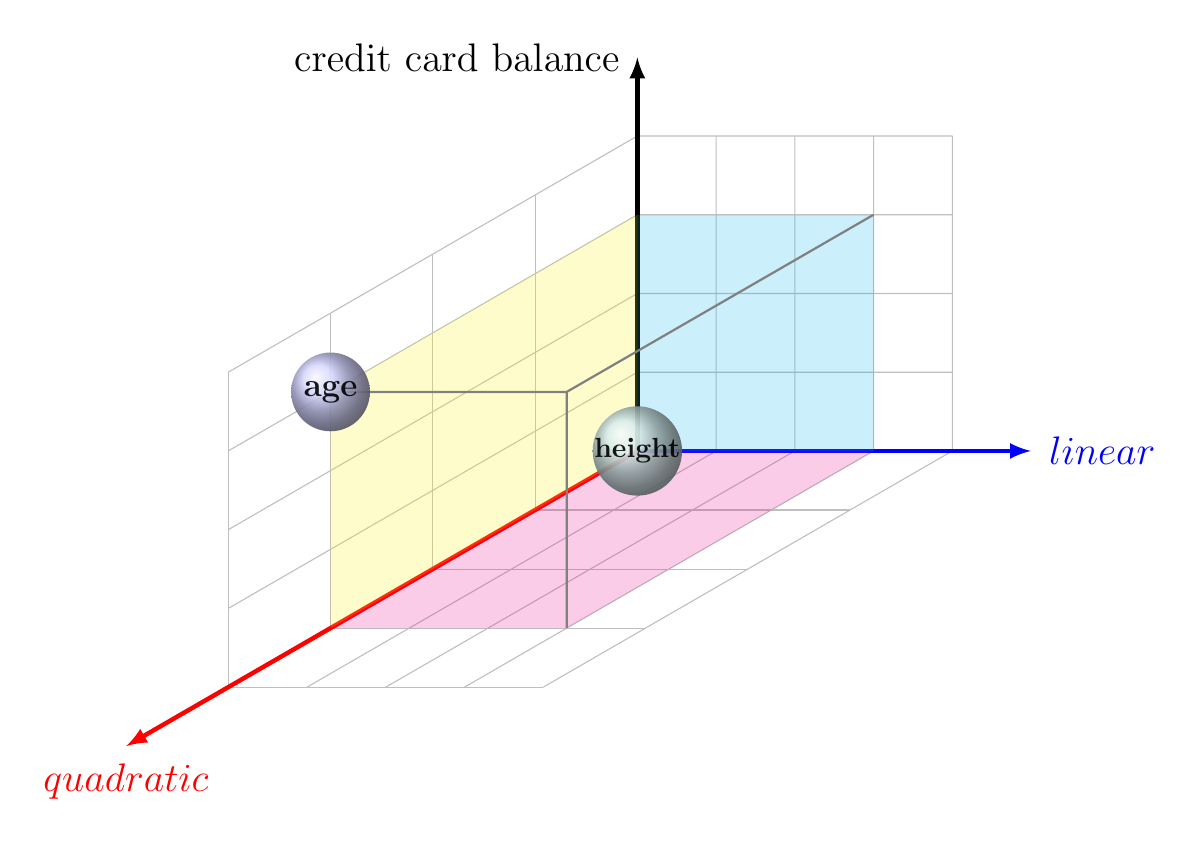
\begin{tikzpicture}[inner sep=0.2cm]
				\def \radi{4}
				\def \x{3}
				\def \y{3}
				\def \z{3}
				
				\begin{scope}[isometricYXZ]
				% the grid
				\begin{scope}[color=gray!50, thin]
				\foreach \xi in {0,...,\radi}{ \draw (\xi,\radi,0) -- (\xi,0,0) -- (\xi,0,\radi); }%
				\foreach \yi in {1,...,\radi}{ \draw (0,\yi,\radi) -- (0,\yi,0) -- (\radi,\yi,0); }%
				\foreach \zi in {0,...,\radi}{ \draw (0,\radi,\zi) -- (0,0,\zi) -- (\radi,0,\zi); }%
				\end{scope}
				
				\draw[-latex, ultra thick, color=blue] (0,0,0) -- (5,0,0) node[anchor=west] {\Large $linear$};%
				\draw[-latex, ultra thick, color=red] (0,0,0) -- (0,5,0) node[anchor=north] {\Large $quadratic$};%
				\draw[-latex, ultra thick, color=black] (0,0,0) -- (0,0,5) node[anchor=east] {\Large credit card balance};%
				
				\fill[color=magenta, opacity=0.2] (0,0,0) -- (\x,0,0) -- (\x,\y,0) -- (0,\y,0) -- cycle; %
				\fill[color=yellow, opacity=0.2] (0,0,0) -- (0,0,\z) -- (0,\y,\z) -- (0,\y,0) -- cycle; %
				\fill[color=cyan, opacity=0.2] (0,0,0) -- (\x,0,0) -- (\x,0,\z) -- (0,0,\z) -- cycle;
				
				\draw[color=gray, thick]%
				(0,\y,\z) -- (\x,\y,\z) -- (\x,\y,0) (\x,\y,\z) -- (\x,0,\z);%
				\end{scope}
				
				%\shade[ball color=yellow] ($\y*(-1.299cm,-0.75cm)+(\x,\z)$) circle (0.1);%
				\node[circle, minimum width=1cm, inner sep=0pt, outer sep=0pt, ball color=blue!20!white,opacity=0.90] (H-1) at ($\y*(-1.299cm,-0.75cm)+(0,\z)$) {\large \bfseries age};
				\node[circle, minimum width=2*\ab cm, inner sep=0pt, outer sep=0pt, ball color=blue!50!green!20!white,opacity=.9] (H-1) at (0,0,0) {\bfseries height};
				\end{tikzpicture}
			}
		}
		\subfloat[Group Lasso \label{fig:2}]{
			\resizebox{200pt}{!}{
				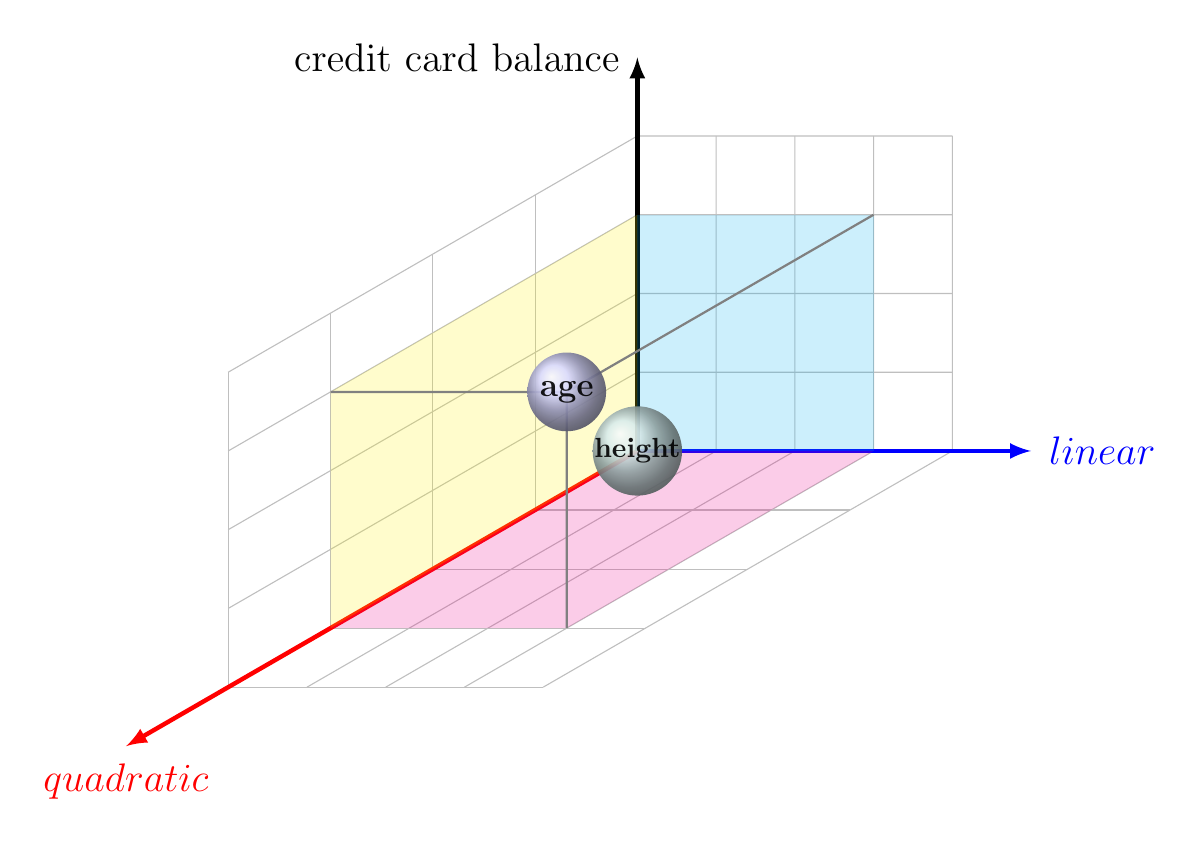
\begin{tikzpicture}[inner sep=0.2cm]
				\def \radi{4}
				\def \x{3}
				\def \y{3}
				\def \z{3}
				
				\begin{scope}[isometricYXZ]
				% the grid
				\begin{scope}[color=gray!50, thin]
				\foreach \xi in {0,...,\radi}{ \draw (\xi,\radi,0) -- (\xi,0,0) -- (\xi,0,\radi); }%
				\foreach \yi in {1,...,\radi}{ \draw (0,\yi,\radi) -- (0,\yi,0) -- (\radi,\yi,0); }%
				\foreach \zi in {0,...,\radi}{ \draw (0,\radi,\zi) -- (0,0,\zi) -- (\radi,0,\zi); }%
				\end{scope}
				
				\draw[-latex, ultra thick, color=blue] (0,0,0) -- (5,0,0) node[anchor=west] {\Large $linear$};%
				\draw[-latex, ultra thick, color=red] (0,0,0) -- (0,5,0) node[anchor=north] {\Large $quadratic$};%
				\draw[-latex, ultra thick, color=black] (0,0,0) -- (0,0,5) node[anchor=east] {\Large credit card balance};%
				
				\fill[color=magenta, opacity=0.2] (0,0,0) -- (\x,0,0) -- (\x,\y,0) -- (0,\y,0) -- cycle; %
				\fill[color=yellow, opacity=0.2] (0,0,0) -- (0,0,\z) -- (0,\y,\z) -- (0,\y,0) -- cycle; %
				\fill[color=cyan, opacity=0.2] (0,0,0) -- (\x,0,0) -- (\x,0,\z) -- (0,0,\z) -- cycle;
				
				\draw[color=gray, thick]%
				(0,\y,\z) -- (\x,\y,\z) -- (\x,\y,0) (\x,\y,\z) -- (\x,0,\z);%
				\end{scope}
				
				%\shade[ball color=yellow] ($\y*(-1.299cm,-0.75cm)+(\x,\z)$) circle (0.1);%
				\node[circle, minimum width=1cm, inner sep=0pt, outer sep=0pt, ball color=blue!20!white,opacity=0.90] (H-1) at ($\y*(-1.299cm,-0.75cm)+(\x,\z)$) {\large \bfseries age};
				\node[circle, minimum width=2*\ab cm, inner sep=0pt, outer sep=0pt, ball color=blue!50!green!20!white,opacity=.9] (H-1) at (0,0,0) {\bfseries height};
				\end{tikzpicture}
			}
			
		}
		\caption{Visualizing the key difference between the lasso and group lasso penalties}\label{fig:lasso_grouplasso_comparison}
\end{figure}


This description follows mainly Yang and Zou (2015). We add the weight matrix.

\subsection{Model}
Only the third term of the log-likelihood~\eqref{eq:loglikrowrank} depends on $\bbeta$:
\begin{equation}
\frac{1}{2} \left\lbrace \left(\bY - \bX\bbeta \right)^T  \left[\frac{1}{\sigma^2(1-\eta)}\left(  \bI_{N_T} - \bU_1 \left(\frac{1-\eta}{\eta}\bSigma_1^{-1} + \bI_{k}\right) ^{-1}\bU_1^T \right)  \right] \left(\bY - \bX\bbeta \right)  \right\rbrace \label{eq:likeW}
\end{equation}
Equation~\eqref{eq:likeW} can be written more generally as
\[
L(\bbeta\mid\bD)=\frac{1}{2}\left[\bY-\widehat{\bY}\right]^{\top}\mathbf{W}\left[\bY-\widehat{\bY}\right]
\]
where $\widehat{\bY}=\sum_{j=1}^{p}\beta_{j}X_{j}$, $\bD$ is the working data $\lbrace \bY, \bX \rbrace$, and $\bW$ is an $N_T \times N_T$ weight matrix given by
\begin{equation}
\bW = \frac{1}{\sigma^2(1-\eta)}\left(  \bI_{N_T} - \bU_1 \left(\frac{1-\eta}{\eta}\bSigma_1^{-1} + \bI_{k}\right) ^{-1}\bU_1^T \right)   \label{eq:weight}
\end{equation}

%Consider the linear regression problem where we have a continuous response $\by\in\mathbb{R}^{n}$
%and let $\bX$ be the design matrix with $n$ rows and $p$ columns where $n$ is the sample size of the raw data. If an intercept is used in the model, we let the first column of $\bX$ be a vector of 1.
Assume that we the predictors in the design matrix $\bX \in \mathbb{R}^{N_T \times p}$ belong to $K$ groups and that the group membership is already defined such that $(1,2,\ldots,p)=\bigcup_{k=1}^{K}I_{k}$ and the cardinality of index set $I_{k}$ is $p_{k}$, $I_{k}\bigcap I_{k^{\prime}}=\emptyset$ for $k\neq k^{\prime},1\le k,k^{\prime}\le K$. Thus group $k$ contains $p_{k}$ predictors, which are $x_{j}$'s for $j\in I_{k}$, and $1\le k\le K.$ If an intercept is included, then $I_{1}=\{1\}$. Given the group partition, we use $\bbeta_{(k)}$ to denote the segment of $\bbeta$ corresponding to group $k$. This notation is used for any $p$-dimensional vector.
%In a more compact form, and introducing observation weights
%\[
%L(\bbeta\mid\bD)=\frac{1}{2}\left[Y-\hat{Y}\right]^{\top}\mathbf{W}\left[Y-\hat{Y}\right]
%\]
%where $\hat{Y}=\sum_{j=1}^{p}\beta_{j}X_{j}$, $\bD$ is the working data $\lbrace \by, \bX \rbrace$, $\bW$ is an $N_T \times N_T$ weight matrix. Then the problem we consider can be expressed as
We consider the group lasso penalized estimator
\begin{equation}
\min_{\bbeta}L(\bbeta \mid \bD)+\lambda\sum_{k=1}^{K}w_{k}\|\bbk\|_{2},\label{eq:wlslasso}
\end{equation}

The loss function $L$ satisfies the quadratic majorization (QM) condition, since there exists
a $p\times p$ matrix $\bH=\bX^{\trans}\mathbf{W}\bX$, and $\nabla L(\bbeta|\bD)=-\left(Y-\hat{Y}\right)^{\top}\mathbf{W}\bX$, which may only depend on the data $\bD$, such that for all $\bbeta,\bbeta^{*}$,
\begin{equation}
L(\bbeta\mid\bD)\le L(\bbeta^{*}\mid\bD)+(\bbeta-\bbeta^{*})^{\trans}\nabla L(\bbeta^{*}|\bD)+\frac{1}{2}(\bbeta-\bbeta^{*})^{\trans}\bH(\bbeta-\bbeta^{*}).\label{QM1}
\end{equation}

\subsection{Algorithm}

Noticing that the penalty term $\sum_{k=1}^{K}w_{k}||\bbeta_{(k)}||_{2}$ is separable with respect to the indices of the features $k=1, \ldots, K$, we can derive the \textit{groupwise-majorization-descent} (GMD) algorithm for computing the solution of~\eqref{eq:wlslasso} when the loss function satisfies the QM condition. Let $\widetilde{\bbeta}$ denote the current solution of $\bbeta$. Without loss of generality, let us derive the GMD update of $\bbkt$, the coefficients of group $k$. Define $\bH_{k}$ as the sub-matrix of $\bH$ corresponding to group $k$. For example, if group 2 is $\{2,4\}$ then $\bH_{(2)}$ is a $2\times2$ matrix with
\[
\bH_{(2)}=\left[\begin{array}{cc}
h_{2,2} & h_{2,4}\\
h_{4,2} & h_{4,4}
\end{array}\right],
\]

where $h_{i,j}$ is the $i,j$th entry of the $\bH$ matrix. Write $\bbeta$ such that $\bbeta_{(k^{\prime})}=\widetilde{\bbeta}_{(k^{\prime})}$ for $k^{\prime}\ne k$. Given $\bbeta_{(k^{\prime})}=\widetilde{\bbeta}_{(k^{\prime})}$ for $k^{\prime}\ne k$, the optimal $\bbk$ is defined as
\begin{equation}
\arg\min_{\boldsymbol{\beta}^{(k)}}L(\bbeta\mid\bD)+\lambda w_{k}\Vert\bbk\Vert_{2}.\label{GMDeq1}
\end{equation}
Unfortunately, there is no closed form solution to~\eqref{GMDeq1} for a general loss function with general design matrix. We overcome the computational obstacle by taking advantage of the QM condition. From~\eqref{QM1} we have
\[
L(\bbeta\mid\bD)\le L(\widetilde{\bbeta}\mid\bD)+(\bbeta-\widetilde{\bbeta})^{\trans}\nabla L(\widetilde{\bbeta}|\bD)+\frac{1}{2}(\bbeta-\widetilde{\bbeta})^{\trans}\bH(\bbeta-\widetilde{\bbeta}).
\]

Write $U(\widetilde{\bbeta})=-\nabla L(\widetilde{\bbeta}|\bD)$. Using
\[
\bbeta-\widetilde{\bbeta}=(\underbrace{0,\ldots,0}_{k-1},\bbk-\bbkt,\underbrace{0,\ldots,0}_{K-k}),
\]
we can write
\begin{equation}
L(\bbeta\mid\bD)\le L(\widetilde{\bbeta}\mid\bD)-(\bbk-\bbkt)^{\trans}U_{(k)}+\frac{1}{2}(\bbk-\bbkt)^{\trans}\bH_{(k)}(\bbk-\bbkt).\label{GMDeq2}
\end{equation}
where
\begin{align}
U_{(k)} & =\frac{\partial}{\partial\bbk}L_{Q}(\bbeta\mid\bD)=-\left(Y-\hat{Y}\right)^{\top}\mathbf{W}\mathbf{X}_{(k)},\label{eq:gradientj-1}\\
\mathbf{H}_{(k)} & =\frac{\partial^{2}}{\partial\bbk\partial\bbk^{\top}}L_{Q}(\bbeta\mid\bD)=\mathbf{X}_{(k)}^{\top}\mathbf{W}\mathbf{X}_{(k)}.\label{eq:hessianj-1}
\end{align}

Let $\eta_{k}$ be the largest eigenvalue of $\bH_{(k)}$. We set $\gamma_{k}=(1+\varepsilon^{*})\eta_{k}$, where $\varepsilon^{*}=10^{-6}$. Then we can further relax the upper bound in~\eqref{GMDeq2} as
\begin{equation}
L(\bbeta\mid\bD)\leq L(\widetilde{\bbeta}\mid\bD)-(\bbeta^{(k)}-\widetilde{\bbeta}^{(k)})^{\trans}U_{(k)}+\frac{1}{2}\gamma_{k}(\bbeta^{(k)}-\widetilde{\bbeta}^{(k)})^{\trans}(\bbeta^{(k)}-\widetilde{\bbeta}^{(k)}).\label{GMDeq3-1}
\end{equation}
It is important to note that the inequality strictly holds unless for $\bbeta^{(k)}=\widetilde{\bbeta}^{(k)}$. Instead of minimizing~\eqref{GMDeq1} we solve
\begin{equation}
\arg\min_{\bbeta^{(k)}}L(\widetilde{\bbeta}\mid\bD)-(\bbeta^{(k)}-\widetilde{\bbeta}^{(k)})^{\trans}U_{(k)}+\frac{1}{2}\gamma_{k}(\bbeta^{(k)}-\widetilde{\bbeta}^{(k)})^{\trans}(\bbeta^{(k)}-\widetilde{\bbeta}^{(k)})+\lambda w_{k}\Vert\bbeta^{(k)}\Vert_{2}.\label{GMDeq4-1}
\end{equation}

Denote by $\widetilde{\bbeta}^{(k)}(\textrm{new})$ the solution to~\eqref{GMDeq4-1}. It is straightforward to see that $\widetilde{\bbeta}^{(k)}(\textrm{new})$ has a simple closed-from expression
\begin{equation}
\widetilde{\bbeta}^{(k)}(\textrm{new})=\frac{1}{\gamma_{k}}\left(U^{(k)}+\gamma_{k}\widetilde{\bbeta}^{(k)}\right)\left(1-\frac{\lambda w_{k}}{\Vert U^{(k)}+\gamma_{k}\widetilde{\bbeta}^{(k)}\Vert_{2}}\right)_{+}.\label{GMDeq5-1}
\end{equation}

Algorithm~\ref{alg1} summarizes the details of GMD.

\begin{algorithm}
	\begin{enumerate}
		\item For $k=1,\ldots,K$, compute $\gamma_k$, the largest eigenvalue of $\bH^{(k)}$.
		\item Initialize $\widetilde \bbeta$.
		\item Repeat the following cyclic groupwise updates until convergence:
		\begin{enumerate}
			\item[---] for $k=1,\ldots,K$, do step (3.1)--(3.3)
			\begin{enumerate}
				\item[3.1]
				Compute $U(\widetilde \bbeta )=-\nabla L(\widetilde \bbeta | \bD)$.
				\item[3.2]
				Compute
				$
				\widetilde \bbeta^{(k)}(\textrm{new}) = \frac{1}{\gamma_k}\left( U^{(k)}+\gamma_k \widetilde \bbeta^{(k)} \right)\left(1-\frac{\lambda w_k}{\Vert U^{(k)}+\gamma_k \widetilde \bbeta^{(k)} \Vert_2}\right)_{+} .
				$
				\item[3.3]
				Set $\widetilde \bbeta^{(k)}=\widetilde \bbeta^{(k)}(\textrm{new})$.
			\end{enumerate}
		\end{enumerate}
	\end{enumerate}
	\caption{The GMD algorithm for general group-lasso learning. \label{alg1}}
\end{algorithm}


\subsection{Convergence}

We can prove the strict descent property of GMD by using the MM principle \citep{MM1,hunter2004tutorial,MM08}. Define
\begin{equation}
Q(\bbeta \mid \bD)=L(\widetilde \bbeta \mid \bD)-(\bbeta^{(k)}-\widetilde \bbeta^{(k)})^{\trans}
U^{(k)}+\frac{1}{2} \gamma_k (\bbeta^{(k)}-\widetilde \bbeta^{(k)})^{\trans} ( \bbeta^{(k)}- \widetilde \bbeta^{(k)})+\lambda w_k \Vert \bbeta^{(k)}\Vert_2.
\end{equation}
Obviously, $Q(\bbeta \mid \bD)=L(\bbeta \mid \bD)+\lambda w_k \Vert \bbeta^{(k)}\Vert_2$ when $\bbeta^{(k)}=\widetilde \bbeta^{(k)}$ and
(\ref{GMDeq3}) shows that
$Q(\bbeta \mid \bD) > L(\bbeta \mid \bD)+\lambda w_k \Vert \bbeta^{(k)}\Vert_2$ when $\bbeta^{(k)} \neq \widetilde \bbeta^{(k)}$.
After updating $\widetilde \bbeta^{(k)}$ using (\ref{GMDeq5}), we have
\begin{eqnarray*}
	L(\widetilde \bbeta^{(k)}(\textrm{new}) \mid \bD)+\lambda w_k \Vert \widetilde \bbeta^{(k)}(\textrm{new}) \Vert_2
	&  \le &  Q(\widetilde \bbeta^{(k)}(\textrm{new})  \mid \bD)\\
	& \le & Q(\widetilde \bbeta  \mid \bD) \\
	& = & L(\widetilde \bbeta \mid \bD)+\lambda w_k \Vert \widetilde \bbeta^{(k)}\Vert_2.
\end{eqnarray*}
Moreover, if $\widetilde \bbeta^{(k)}(\textrm{new}) \neq \widetilde \bbeta^{(k)}$, then the first inequality becomes
\begin{eqnarray*}
	L(\widetilde \bbeta^{(k)}(\textrm{new}) \mid \bD)+\lambda w_k \Vert \widetilde \bbeta^{(k)}(\textrm{new}) \Vert_2
	&  < &  Q(\widetilde \bbeta^{(k)}(\textrm{new})  \mid \bD).
\end{eqnarray*}
Therefore, the objective function is strictly decreased after updating all groups in a cycle, unless the solution does not change after each groupwise update. If this is the case,
we can show that the solution must satisfy the KKT conditions, which means that the algorithm converges and finds the right answer. To see this,
if $\widetilde \bbeta^{(k)}(\textrm{new}) = \widetilde \bbeta^{(k)}$ for all $k$, then by the update formula \eqref{GMDeq5-1} we have that for all $k$
\begin{align}\label{KKTcond1}
\widetilde \bbeta^{(k)} = \frac{1}{\gamma_k}\left( U^{(k)}+\gamma_k \widetilde \bbeta^{(k)} \right)\left(1-\frac{\lambda w_k}{\Vert U^{(k)}+\gamma_k \widetilde \bbeta^{(k)} \Vert_2}\right) \qquad\textrm{if }\Vert U^{(k)}+\gamma_k \widetilde \bbeta^{(k)} \Vert_2 > \lambda w_{k},\\\label{KKTcond2}
\widetilde \bbeta^{(k)} = \boldsymbol{0} \qquad\textrm{if }\Vert U^{(k)}+\gamma_k \widetilde \bbeta^{(k)} \Vert_2 \leq \lambda w_{k}.
\end{align}
By straightforward algebra  we obtain the KKT conditions:
\begin{align*}
-U^{(k)}+\lambda w_{k}\cdot\frac {\widetilde\bbeta^{(k)} }{\Vert\widetilde\bbeta^{(k)}\Vert_2}=\boldsymbol{0}\qquad\textrm{if }\widetilde\bbeta^{(k)}\neq \boldsymbol{0},\\
\left\Vert
U^{(k)}
\right\Vert_2 \le\lambda w_{k}\qquad\textrm{if }\widetilde\bbeta^{(k)}=\boldsymbol{0},
\end{align*}
where $k=1,2,\ldots,K$. Therefore, if the objective function stays unchanged after a cycle, the algorithm necessarily converges to the right
answer.




\section{Penalized interaction models}


%In the context of studying gene environment interactions, all previously mentioned methods can yield results where the main effects are 0 but the cross terms are not. While there may exist situations where this can occur, such behavior is generally not biologically plausible in genomics~\citep{bakermans2015hidden}. 
%Two other arguments against such behavior have to do with statistical power and practical importance; 1) large main effects are more likely to lead to detectable interactions than small ones~\citep{cox1984interaction} and 2) a data collector cares about the number of variables they need to \textit{measure} to make predictions at a future time~\citep{bien2013lasso}. 
%Moreover, the proposed clustering methods are based on features from all observations. Any correlation patterns specific to a subgroup of patients (e.g. Figures~\ref{fig:COPDnevercorr} and~\ref{fig:COPDcurrentcorr}) may become diluted when looking at the overall correlation matrix. 
%Therefore the focus of my doctoral research will be on developing a method that can identify previously unknown sets of highly correlated genes that interact with the environment to explain phenotypic variation, with a focus on prediction accuracy and model interpretability. 

Then something about other structured L1 penalizations that have been proposed. There are quite a few examples of penalties built for specific applications, and maybe you could find a few such examples and cite them. Not comprehensively.  Then you can point to the sail chapter as a new structured penalty.

\ctable[pos=H,doinside=\footnotesize]{lcc}{
}{
\FL
Type      & Method   & Software \ML
\multicolumn{1}{m{1cm}}{Linear}    & \multicolumn{1}{m{6cm}}{\texttt{CAP}~\citep{zhao2009composite} }        &   \xmark    \\
& \multicolumn{1}{m{4cm}}{\texttt{SHIM}~\citep{choi2010variable}}        &   \xmark    \\
& \multicolumn{1}{m{4cm}}{\texttt{hiernet}~\citep{bien2013lasso}}        &   \texttt{hierNet(x, y)}    \\
& \multicolumn{1}{m{4cm}}{\texttt{GRESH}~\citep{she2014group} }        &  \xmark     \\
& \multicolumn{1}{m{4cm}}{\texttt{FAMILY}~\citep{haris2016convex}}    &  \texttt{FAMILY(x, z, y)}   \\
& \multicolumn{1}{m{4cm}}{\texttt{glinternet}~\citep{lim2015learning} }    & \texttt{glinternet(x, y)}  \\			   	 	
& \multicolumn{1}{m{4cm}}{\texttt{RAMP}~\citep{hao2018model}}        & \texttt{RAMP(x, y)}  \\ 
& \multicolumn{1}{m{4cm}}{\texttt{LassoBacktracking}~\citep{shah2016modelling}   }        & \texttt{LassoBT(x, y)}  \ML
\multicolumn{1}{m{4cm}}{Non-linear} 	& \multicolumn{1}{m{8cm}}{\texttt{VANISH}~\citep{radchenko2010variable} }        & \xmark  \\
& \multicolumn{1}{m{4cm}}{\texttt{sail}}        & \texttt{sail(x, y, e)}  \LL
}

\subsection{Current methods overview and their limitations} \label{subsec:methods-overview2}

We consider a regression model for an outcome variable $Y=(y_1, \ldots, y_n)$ which follows an exponential family. Let $E=(e_1, \ldots, e_n)$ be the binary environment vector and $\bx = (X_{1}, \ldots, X_{p})$ be the matrix of high-dimensional data. Consider the regression model with main effects and their interactions with $E$:
\begin{align}
g(\bmu)  = & \beta_0  + \underbrace{\beta_1 X_{1} + \cdots + \beta_p X_p + \beta_{E} E}_{\tm{main effects}} + \underbrace{\alpha_{1E} (X_1 E) + \cdots + \alpha_{pE} (X_p E)}_{\tm{interactions}} \label{eq:linpred1}
\end{align}
where $g(\cdot)$ is a known link function and $\bmu = \e\left[Y|\bx, E, \bbeta,\balpha\right]$. Our goal is to estimate the parameters \mbox{$\bbeta = \left(\beta_1, \beta_2, \ldots, \beta_p, \beta_E\right) \in \mathbb{R}^{p+1}$} and $\boldsymbol{\alpha} = \left(\alpha_{1E}, \ldots, \alpha_{pE}\right) \in \mathbb{R}^p$ and to improve prediction of $Y$. In fact, in the light of our goals to improve prediction and interpretability, we also consider the related model
\begin{equation}  g(\bmu) = \beta^*_0 + \sum_{k=1}^q \beta^*_k \widetilde{X}_k + \beta^*_E E + 
\sum_{k=1}^q \alpha^*_k E \widetilde{X}_k 
\label{eq:linpred1.1}
\end{equation}
where $\widetilde{X}_k, k=1, \ldots, q$ are linear combinations of $X$ designed to reduce the dimension, such that $q<<p$, and the superscript asterisk on the parameters is just to emphasize that these are different from those in~\eqref{eq:linpred1}. In what follows, we omit the asterisk on the parameters for clarity.


\subsection{Phase 3: Variable Selection} \label{sec:varselect}
%Because the clustering in phase 1 is unsupervised, it is possible that the derived latent representations from phase 2 will not be associated with the response. Therefore we propose to regress the response on the summary measures via penalized likelihood of the form given by \ref{eq:penalisedlikelihood}. These methods are able to simultaneous estimate and select regression parameters. We argue that the selected non-zero predictors in this model will represent clusters of genes that interact with the environment and are associated with the phenotype. Such an additive model might be insufficient for predicting the outcome. In this case we may directly include the environment variable, the summary measures and their interaction. However, since no constraint is placed on the structure of the model in~\ref{eq:penalisedlikelihood}, it is possible that the estimated main effects are zero while the interaction term is not. This has motivated methods that produce structured sparsity~\cite{bach2012structured}. For example, Bien \textit{et al.}~\cite{bien2013lasso} propose a strong hierarchical lasso which forces the main effects to be included if the interaction term is non-zero. However this method and related ones are restricted to all pairwise interactions between $p$ measured variables. Therefore I will explore methods that impose a strong hierarchy in the context of gene environment interactions. 
We are interested in imposing the strong heredity principle~\citep{chipman1996bayesian}: 
\begin{equation}
\hat{\alpha}_{jE} \neq 0 \qquad \Rightarrow \qquad \hat{\beta}_j \neq 0 \qquad \tm{and} \qquad \hat{\beta}_E \neq 0   \label{eq:heredity}
\end{equation}
In words, the interaction term will only have a non-zero estimate if its corresponding main effects are estimated to be non-zero. One benefit brought by hierarchy is that the number of measured variables can be reduced, referred to as practical sparsity~\cite{she2014group,bien2013lasso}. For example, a model involving $X_1, E, X_1 \cdot E$ is more parsimonious than a model involving $X_1, E, X_2 \cdot E$, because in the first model a researcher would only have to measure two variables compared to three in the second model. In order to address these issues, we propose to extend the model of Choi \textit{et al.}~\citep{choi2010variable} to simultaneously perform variable selection, estimation and impose the strong heredity principle in the context of high dimensional interactions with the environment (HD$\times E$). To do so, we follow Choi and reparametrize the coefficients for the interaction terms as $\alpha_{jE} = \gamma_{jE} \beta_j \beta_E$. Plugging this into~\eqref{eq:linpred1}:
\begin{align}
g(\bmu)  = & \beta_0  + \beta_1 \widetilde{X}_{1} + \cdots + \beta_q \widetilde{X}_q + \beta_{E} E + \gamma_{1E}\beta_1 \beta_E (\widetilde{X}_1 E) + \cdots + \gamma_{qE}\beta_q \beta_E (\widetilde{X}_q E)    \label{eq:linpred2}
\end{align}
where $\widetilde{\bx} = (\widetilde{X}_1, \ldots, \widetilde{X}_q)$ are the cluster representatives derived in phase 2 and $q <p$. This reparametrization directly enforces the strong heredity principle (Eq.~\eqref{eq:heredity}), i.e., if either main effect estimates are 0, then $\hat{\alpha}_{jE}$ will be zero and a non-zero interaction coefficient implies non-zero $\hat{\beta}_j$ and $\hat{\beta}_E$. To perform variable selection in this new parametrization, we follow Choi \textit{et al.}~\cite{choi2010variable} and penalize $\bs{\gamma} = \left(\gamma_{1E}, \ldots, \gamma_{pE}\right)$ instead of penalizing $\balpha$ as in~\eqref{eq:lassolikelihood}, leading to the following penalized least squares criterion:
\begin{equation}
\argmin_{\beta_0, \bbeta, \bs{\gamma} }  \frac{1}{2} \norm{Y - g(\bmu)}^2 + \lambda_\beta \left(w_1 \beta_1 + \cdots + w_q \beta_q + w_E \beta_E   \right) + \lambda_\gamma  \left( w_{1E} \gamma_{1E} + \cdots + w_{qE}\gamma_{qE}         \right) \label{eq:lassolikelihood2}
\end{equation} 
where $g(\bmu)$ is from~\eqref{eq:linpred2}, $\lambda_\beta$ and $\lambda_\gamma$ are tuning parameters and $\mb{w} = \left(w_{1}, \ldots, w_q, w_{1E}, \ldots, w_{qE}\right)$ are prespecified adaptive weights. The $\lambda_\beta$ tuning parameter controls the amount of shrinkage applied to the main effects, while $\lambda_\gamma$ controls the interaction estimates and allows for the possibility of excluding the interaction term from the model even if the corresponding main effects are non-zero. The adaptive weights serve as a way of allowing parameters to be penalized differently. Furthermore, adaptive weighting~\citep{zou2006adaptive} has been shown to construct oracle procedures~\citep{fan2001variable}, i.e., asymptotically, it performs as well as if the true model were given in advance. The oracle property is achieved when the weights are a function of any root-$n$ consistent estimator of the true parameters e.g. maximum likelihood (MLE) or ridge regression estimates. It can be shown that the procedure in~\eqref{eq:lassolikelihood2} asymptotically possesses the oracle property~\citep{choi2010variable}, even when the number of parameters tends to $\infty$ as the sample size increases, if the weights are chosen such that
\begin{equation}
w_j = \left | \frac{1}{\hat{\beta}_j} \right|, \quad w_{jE} = \left | \frac{\hat{\beta}_j \hat{\beta}_E}{\hat{\alpha}_{jE}} \right| \quad \tm{ for }j=1, \ldots, q   \label{eq:weights}
\end{equation}
where $\hat{\beta}_j$ and $\hat{\alpha}_{j}$ are the MLEs, \textit{using the transformed variables}, from~\eqref{eq:linpred1} or the ridge regression estimates when $q > n$. The rationale behind the data-dependent $\hat{\bs{w}}$ is that as the sample size grows, the weights for the truly zero predictors go to $\infty$ (which translates to a large penalty), whereas the weights for the truly non-zero predictors converge to a finite constant~\citep{zou2006adaptive}. 

There have been several more recent proposals for modeling interactions with the strong heredity constraint in the variable selection via penalization literature including Composite Absolute Penalties (CAP)~\citep{zhao2009composite}, Variable selection using Adaptive Nonlinear Interaction Structures in High dimensions (VANISH)~\citep{radchenko2010variable}, Strong Hierarchical Lasso (hierNet)~\citep{bien2013lasso}, Group-Lasso Interaction Network (glinternet)~\citep{lim2015learning}, Group Regularized Estimation under Structural Hierarchy (GRESH)~\citep{she2014group} and a Framework for Modeling Interactions with a Convex Penalty (FAMILY)~\citep{haris2014convex}. While each method has their own merit, including that they are all convex optimization problems, they all contain complex penalty functions which are hard to interpret and lead to computationally expensive fitting algorithms. On the other hand, the objective function in~\eqref{eq:lassolikelihood2} can be solved using an iterative approach (by first fixing $\bbeta$ and then $\balpha$) which simplifies to a LASSO type problem; one that has been extensively studied, is well understood and can be solved efficiently using existing software (e.g. \texttt{glmnet}~\citep{friedman2010regularization}). A limitation of this approach is that the optimization problem is non-convex, arising from the reparametrization of $\balpha$ as a product of optimization variables $(\bbeta, \bs{\gamma})$, and hence convergence to the global minimum is not guaranteed~\citep{choi2010variable}. We argue that since there is only one $E$, and that $\widetilde{X}$ is much smaller in dimension, finding a solution is much more likely. 

%We argue here that in our applications, we are more concerned with identifying the truly associated parameters (as given by an oracle procedure) than finding a global minimum which would be guaranteed in a convex formulation. 

To our knowledge, strong hierarchies have never previously been used in HD interaction analysis in genomics or brain imaging studies. Furthermore, the specific choices of weights proposed here, i.e., based on the transformed variables from phase 2, have not been previously used. Choi \textit{et al.}~\citep{choi2010variable} estimated their weights simultaneously, but this would not be feasible in HD data. Finally, the adaptation to interactions with one key $E$ variable is specific to our situation and this leads to computational efficiencies. These three points constitute novel aspects of this thesis. I have a working implementation of this, and am in the process of conducting simulation studies.


\section{Penalized linear mixed models}
(5) A brief intro to linear mixed models followed by why naive penalization violates the normality of residuals to motivate your ggmix chapter.


%\section{you will need a section on things like gradient descent and other algorithms for finding solutions efficiently}
	%-----------------------------------------------------------------------------
\chapter{Sparse Additive Interaction Learning\label{ch:sail}}
%-----------------------------------------------------------------------------

Sahir Rai Bhatnagar$^{1,2}$, Amanda Lovato$^{2}$, Yi Yang$^{3}$, Celia MT Greenwood$^{1,2}$
%\affil[1]{Department of Epidemiology, Biostatistics and Occupational Health, McGill University}
%\affil[2]{Lady Davis Institute, Jewish General Hospital, Montr\'{e}al, QC}
%\affil[3]{Departments of Oncology and Human Genetics, McGill University}
%\affil[4]{Department of Mathematics and Statistics, McGill University}
%\affil[5]{Montreal Neurological Institute, McGill University}
%\affil[6]{Department of Computer Science, McGill University}
%\affil[7]{Department of Biochemistry, Universit\'{e} de Sherbrooke}

%\author{Brian D. Beitzel}
$^{1}$Department of Epidemiology, Biostatistics and Occupational Health, McGill University\\
$^{2}$Lady Davis Institute, Jewish General Hospital, Montr\'{e}al, QC \\
$^{3}$Department of Mathematics and Statistics, McGill University\\



\newpage

\section*{Abstract}
Diseases are now thought to be the result of changes in entire biological networks whose states are affected by a complex interaction of genetic and environmental factors. In general, power to estimate interactions is low, the number of possible interactions could be enormous and their effects may be non-linear. Existing approaches such as the lasso might keep an interaction but remove a main effect, which is problematic for interpretation. We develop a model for linear and non-linear interactions in penalized regression models that automatically enforces the strong heredity property. A computationally efficient fitting algorithm combined with a non-parametric screening approach scales to high-dimensional datasets and has been implemented in an R package. We apply our method to identify gene-prenatal maternal depression interactions on negative emotionality in mother–infant dyads from the Maternal Adversity, Vulnerability, and Neurodevelopment (MAVAN) cohort.

\newpage

\section{Introduction}

Computational approaches to variable selection have become increasingly important with the advent of high-throughput technologies in genomics and brain imaging studies, where the data has become massive, yet where it is believed that the number of truly important variables is small relative to the total number of variables. 
Although many approaches have been developed for main effects, there is an enduring interest in powerful methods for estimating interactions, since interactions may reflect important modulation of a genomic system by an external factor~\citep{bhatnagar2018analytic}. 
Accurate capture of interactions may hold the potential to better understanding  biological phenomena and improving prediction accuracy. 
For example, a model that considered interactions between brain imaging data and genetic features had better classification accuracy compared to a model that considered the main effects only~\citep{ning2018classifying}. 
%For example, genome wide association studies (GWAS) have been unable to explain a large proportion of heritability (the variance in phenotype attributable to genetic variants) and it has been suggested that this missing heritability may in part be due to gene-environment interactions~\citep{manolio2009finding}. 
Furthermore, the manifestations of disease are often considered to be the result of changes in entire biological networks whose states are affected by a complex interaction of genetic and environmental factors~\citep{schadt2009molecular}. 
However, there is a general deficit of such replicated interactions in the literature~\citep{timpson2018genetic}.   
Indeed, power to detect interactions is always lower than for  main effects, and in high-dimensional settings ($p >> n$), this lack of power to detect interactions is exacerbated, since the number of possible interactions could be enormous and their effects may be non-linear. Hence, analytic methods that may improve power are essential.  

%{\color{green} You need a non-genetic example - i.e. gene expression or proteomic or ...}
Interactions may occur in numerous types and of varying complexities. In this paper, we consider one specific type of interaction models, where one (exposure) variable is involved in possibly non-linear interactions with a high-dimensional set of measures $\mb{X}$ leading to effects on a response variable, $Y$. We propose a multivariable penalization procedure for detecting non-linear interactions $\mb{X}$ and $E$. 


%Our approach improves on existing procedures for detecting such interactions in three ways; 1) it automatically enforces the strong heredity property, i.e., an interaction term can only be included in the model if the corresponding main effects are in the model 2) it reduces the dimensionality of the problem and leverages the high correlations by transforming the input feature space using network connectivity measures and 3) it leads to interpretable models which are biologically meaningful.


%Furthermore, diseases are now thought to be the result of entire biological networks whose states are affected by environmental factors, and these systemic changes can induce or eliminate strong correlations between elements in a network. Therefore, we propose a multivariate penalization procedure for detecting interactions between high dimensional data ($p >> n$) and an environmental factor, where the effect of this environmental factor on the high dimensional data is widespread and plays a role in predicting the response. Our approach improves on existing procedures for detecting such interactions in three ways; 1) it automatically enforces the strong heredity property, i.e., an interaction term can only be included in the model if the corresponding main effects are in the model 2) it reduces the dimensionality of the problem and leverages the high correlations by transforming the input feature space using network connectivity measures and 3) it leads to interpretable models which are biologically meaningful. This thesis is motivated by three studies; one that looks at the impact of maternal care on child development, another that characterizes normal brain development as a function of intelligence scores and one that looks at the long-lasting effects of diet in subsequent generations.


%Diseases are now thought to be the result of changes in entire biological networks whose states are affected by a complex interaction of genetic and environmental factors. In general, power to estimate interactions is low, the number of possible interactions could be enormous and their effects may be non-linear. Existing approaches such as the lasso might keep an interaction but remove a main effect, which is problematic for interpretation. We develop a model for linear and non-linear interactions in penalized regression models that automatically enforces the strong heredity property. A computationally efficient fitting algorithm combined with a non-parametric screening approach scales to high-dimensional datasets and has been implemented in an R package. We apply our method to identify gene-prenatal maternal depression interactions on negative emotionality in mother–infant dyads from the Maternal Adversity, Vulnerability, and Neurodevelopment (MAVAN) cohort.



\subsection{A Sparse additive interaction model}
Let $Y=(Y_1, \ldots, Y_n) \in \mathbb{R}^n$ be a continuous outcome variable, \mbox{$X_E=(E_1, \ldots, E_n) \in \mathbb{R}^n$} a binary or continuous environment vector, and \mbox{$\bX = (X_{1}, \ldots, X_{p}) \in \mathbb{R}^{n\times p}$} a matrix of predictors, possibly high-dimensional. Furthermore let $f_j: \mathbb{R} \rightarrow \mathbb{R}$ be a smoothing method for variable $X_j$ by a projection on to a set of basis functions:
\begin{equation}
f_j(X_j) = \sum_{\ell = 1}^{m_j} \psi_{j\ell}(X_j) \beta_{j\ell} \label{eq:smooth}
\end{equation}
Here, the $\left\lbrace \psi_{j\ell} \right\rbrace_1^{m_j}$ are a family of basis functions in $X_j$~\citep{hastie2015statistical}. Let $\bPsi_j$ be the $n \times m_j$ matrix of evaluations of the $\psi_{j\ell}$ and \mbox{$\btheta_j = (\beta_{j1}, \ldots, \beta_{jm_j}) \in \mathbb{R}^{m_j}$} for $j = 1, \ldots, p$ ($\btheta_j$ is a $m_j$-dimensional column vector of basis coefficients for the $j$th main effect). In this article we consider an additive interaction regression model of the form 
\begin{align}
g(\bmu)  & =  \beta_0 \cdot \boldsymbol{1} + \sum_{j=1}^p \bPsi_j \btheta_j + \beta_E X_E + \sum_{j=1}^p (X_E \circ \bPsi_j) \btau_{j}    \label{eq:linpred}
\end{align}
where $g(\cdot)$ is a known link function, $\bmu = \e\left[Y|\bPsi, X_E \right]$, $\beta_0$ is the intercept, $\beta_E$ is the coefficient for the environment variable, $\btau_j = (\tau_{j1}, \ldots, \tau_{jm_j})\in \mathbb{R}^{m_j}$ are the basis coefficients for the $j$th interaction term, and $(X_E \circ \bPsi_j)$ is the $n \times m_j$ matrix formed by the component-wise multiplication of the column vector $X_E$ by each column of $\bPsi_j$. For a continuous response, we use the squared-error loss to estimate the parameters:
\begin{equation}
\mathcal{L}(\bTheta| \bD) = \frac{1}{2n}\norm{Y - \beta_0 \cdot \boldsymbol{1} - \sum_{j=1}^p \bPsi_j \btheta_j - \beta_E X_E - \sum_{j=1}^p (X_E \circ \bPsi_j) \btau_j }_2^2
\end{equation}
and for binary response $Y_i \in \left\lbrace -1, +1 \right\rbrace$ we use the logistic loss:
\begin{equation}
\mathcal{L}(\bTheta| \bD) = \frac{1}{n} \sum_i \log \left(1 + \exp \left\lbrace - Y_i \left( \beta_0 \cdot \boldsymbol{1} - \sum_{j=1}^p \bPsi_j \btheta_j - \beta_E X_E - \sum_{j=1}^p (X_E \circ \bPsi_j) \btau_j \right) \right\rbrace   \right)
\end{equation}

where $\bTheta \coloneqq (\beta_0, \beta_E,\btheta_1, \ldots, \btheta_p, \btau_1, \ldots, \btau_p)$ and $\bD \coloneqq (Y,\bPsi,X_E)$ is the working data. Here we assume that $p$ is large relative to $n$, and particularly that $\sum_{j=1}^{p}m_j / n$ is large.
Due to the large number of parameters to estimate with respect to the number of observations, one commonly-used approach is to shrink the regression coefficients by placing a constraint on the values
of $(\beta_E, \btheta_j, \btau_j)$. Certain constraints have the added benefit of producing a sparse model in the sense that many of the coefficients will be set exactly to 0~\citep{buhlmann2011statistics}. Such a reduced predictor set can lead to a more interpretable model with smaller prediction variance, albeit at the cost of having biased parameter estimates~\citep{fan2014challenges}. In light of these goals, we consider the following objective function:
\begin{equation}
\argmin_{\bTheta }  	\mathcal{L}(\bTheta| \bD) + \lambda (1-\alpha)  \left( w_E \abs{\beta_E} + \sum_{j=1}^{p} w_j \norm{\btheta_j}_2 \right) +  \lambda\alpha \sum_{j=1}^{p} w_{jE} \norm{\btau_{j}}_2 \label{eq:lassolikelihood3}
\end{equation} 
where $\norm{\btheta_j}_2 = \sqrt{\sum_{k=1}^{m_j} \beta_{jk}^2}$, $\norm{\btau_j}_2 = \sqrt{\sum_{k=1}^{m_j} \tau_{jk}^2}$, $\lambda >0$ and $\alpha \in (0,1)$ are adjustable tuning parameters, $w_E, w_j, w_{jE}$ are non-negative penalty factors for $j=1, \ldots, p$ which serve as a way of allowing parameters to be penalized differently. The first term in the penalty penalizes the main effects while the second term penalizes the interactions. The parameter $\alpha$ controls the relative weight on the two penalties. Note that we do not penalize the intercept. 

An issue with~\eqref{eq:lassolikelihood3} is that since no constraint is placed on the structure of the model, it is possible that an estimated interaction term is nonzero while the corresponding main effects are zero. While there may be certain situations where this is plausible, statisticians have generally argued that interactions should only be included if the corresponding main effects are also in the model~\citep{mccullagh1989generalized}. This is known as the strong heredity principle~\citep{chipman1996bayesian}. Indeed, large main effects are more likely to lead to detectable interactions~\citep{cox1984interaction}. In the next section we discuss how a simple reparametrization of the model~\eqref{eq:lassolikelihood3} can lead to this desirable property. 
%Furthermore, adaptive weighting~\citep{zou2006adaptive} has been shown to construct oracle procedures~\citep{fan2001variable}, i.e., asymptotically, it performs as well as if the true model were given in advance. These weights are given by
%\begin{equation}
%	w_E = \left|   \frac{1}{\hat{\beta}_E} \right| ,\quad w_j = \frac{1}{\norm{\hat{\btheta}_j}_2} , \quad w_{jE} = \left | \frac{\hat{\beta}_E \norm{\hat{\btheta}_j}_2}{\norm{\hat{\alpha}_{j}}_2} \right| \quad \tm{ for }j=1, \ldots, p   \label{eq:weights}
%\end{equation}
%where $\hat{\beta}_E$, $\hat{\btheta}_j$ and $\hat{\balpha}_{j}$ are the MLEs, from~\eqref{eq:linpred} or the ridge regression estimates when $p > n$.

\subsection{Strong and weak heredity}

The strong heredity principle states that an interaction term can only have a non-zero estimate if its corresponding main effects are estimated to be non-zero. The weak heredity principle allows for a non-zero interaction estimate as long as one of the corresponding main effects is estimated to be non-zero~\citep{chipman1996bayesian}. In the context of penalized regression methods, these principles can be formulated as structured sparsity \citep{bach2012structured} problems. Several authors have proposed to modify the type of penalty in order to achieve the heredity principle~\citep{radchenko2010variable,bien2013lasso,haris2014convex,lim2014learning}. We take an alternative approach. Following Choi et al.~\citep{choi2010variable}, we introduce a new set of parameters $\bgamma = (\gamma_1, \ldots, \gamma_p)\in \mathbb{R}^p$ and reparametrize the coefficients for the interaction terms $\btau_j$ in~\eqref{eq:linpred} as a function of $\gamma_j$ and the main effect parameters $\btheta_j$ and $\beta_E$. This reparametrization for both strong and weak heredity is summarized in Table~\ref{tab:reparam}.

\ctable[caption={Reparametrization for strong and weak heredity principle for \texttt{sail} model},label=tab:reparam,pos=h!,doinside=\footnotesize, ]{lll}{
}{
\FL
Type      & Feature  & Reparametrization \ML
\multicolumn{1}{m{3cm}}{Strong heredity}    & \multicolumn{1}{m{5cm}}{$\hat{\btau}_{j} \neq 0 \Rightarrow  \hat{\btheta}_j \neq 0  \tm{ and }  \hat{\beta}_E \neq 0$}        &   $\btau_{j} = \gamma_{j} \beta_E \btheta_j $    \\
\multicolumn{1}{m{3cm}}{Weak heredity} & \multicolumn{1}{m{5cm}}{$\hat{\btau}_{j} \neq 0 \Rightarrow  \hat{\btheta}_j \neq 0  \tm{ or }  \hat{\beta}_E \neq 0$}        &   $\btau_{j} = \gamma_{j}(\beta_E \cdot \mb{1}_{m_j} +  \btheta_j)$    \LL
}


To perform variable selection in this new parametrization, we penalize $\bs{\gamma} = \left(\gamma_{1}, \ldots, \gamma_{p}\right)$ instead of penalizing $\btau$ as in~\eqref{eq:lassolikelihood3}, leading to the following objective function:
\begin{equation}
\argmin_{\bTheta }  	\mathcal{L}(\bTheta| \bD) + \lambda (1-\alpha)  \left( w_E \abs{\beta_E} + \sum_{j=1}^{p} w_j \norm{\btheta_j}_2 \right) +  \lambda\alpha \sum_{j=1}^{p} w_{jE} \abs{\gamma_{j}} \label{eq:saillikelihood}
\end{equation}
%where
%\begin{equation}
%	\mathcal{L}(\bTheta| \bD) = \frac{1}{2n}\norm{Y - \beta_0 \cdot \boldsymbol{1} - \sum_{j=1}^p \bPsi_j \btheta_j - \beta_E X_E - \sum_{j=1}^p (X_E \circ \bPsi_j) \btau_j }_2^2
%\end{equation}
%for a continuous response, and 
%\begin{equation}
%	\mathcal{L}(\bTheta| \bD) = \frac{1}{n} \sum_i \log \left(1 + \exp \left\lbrace - Y_i \left( \beta_0 \cdot \boldsymbol{1} - \sum_{j=1}^p \bPsi_j \btheta_j - \beta_E X_E - \sum_{j=1}^p (X_E \circ \bPsi_j) \btau_j \right) \right\rbrace   \right)
%\end{equation}
%for a binary response. 
This penalty allows for the possibility of excluding the interaction term from the model even if the corresponding main effects are non-zero. Furthermore, smaller values for $\alpha$ would lead to more interactions being included in the final model while values approaching 1 would favor main effects. 
Similar to the elastic net~\citep{zou2005regularization}, we fix $\alpha$ and obtain a solution path over a sequence of $\lambda$ values. 

\subsection{Toy example}

We present here a toy example to better illustrate our method. With a sample size of $n=100$, we sample $p=20$ covariates $X_1, \ldots X_p$ independently from a $N(0,1)$ distribution truncated to the interval [0,1]. Data were generated from a model which follows the strong heredity principle, but where only one covariate, $X_2$, is involved in an interaction with a binary exposure variable, $E$:
\begin{equation}
Y = f_1(X_1) + f_2(X_2) + 1.75 E + 1.5 E \cdot f_2(X_2) + \varepsilon
\end{equation}
For illustration, function $f_1(\cdot)$ is assumed to be linear, whereas function $f_2(\cdot)$ is non-linear: $f_1(x) = -3x$, $f_2(x) = 2(2x-1)^3$. The error term $\varepsilon$ is generated from a normal distribution with variance chosen such that the signal-to-noise ratio (SNR) is 2.  We generated a single simulated dataset and used the strong heredity \sail ~method with cubic B-splines to estimate the functional forms. 10-fold cross-validation (CV) was used to choose the optimal value of penalization. We used $\alpha=0.5$ and default values were used for all other arguments. We plot the solution path for both main effects and interactions in Figure~\ref{fig:toy-solution-path}, coloring lines to correspond to the selected model. We see that our method is able to correctly identify the true model. We can also visually see the effect of the penalty and strong heredity principle working in tandem, i.e., the interaction term $E \cdot f_2(X_2)$ (orange lines in the bottom panel) can only be nonzero if the main effects $E$ and $f_2(X_2)$ (black and orange lines respectively in the top panel) are nonzero, while nonzero main effects doesn't necessarily imply a nonzero interaction. 

\fig{toy-solution-path-1}{toy-solution-path}{16cm}{Toy example solution path for main effects (top) and interactions (bottom). $\left\lbrace X1_1, X1_2, X1_3 \right\rbrace$ and $\left\lbrace X2_1, X2_2, X2_3 \right\rbrace$ are the three basis coefficients for $X_1$ and $X_2$, respectively. $\lambda_{1SE}$ is the largest value of penalization for which the CV error is within one standard error of the minimizing value $\lambda_{min}$.}{Toy example solution path for \sail ~method.}



In Figure~\ref{fig:toy-effects}, we plot the true and estimated component functions $\hat{f}_1(X_1)$ and $E \cdot \hat{f}_2(X_2)$, and their estimates from this analysis with \texttt{sail}. We are able to capture the shape of the correct functional form, but the means are not well aligned with the data. Lack-of-fit for $f_1(X_1)$ can be partially explained by acknowledging that \sail ~is trying to fit a cubic spline to a linear function. Nevertheless, this example demonstrates that \sail ~can still identify trends reasonably well. 


\fig{toy-effects-1}{toy-effects}{16cm}{Estimated smooth functions for $X_1$ and the $X_2 \cdot E$ interaction by the \texttt{sail} method based on $\lambda_{min}$.}{Estimated smooth functions for $X_1$ and the $X_2 \cdot E$ interaction by the \texttt{sail} method based on $\lambda_{min}$.}



\subsection{Related Work}
Methods for variable selection of interactions can be broken down into two categories: linear and non-linear interaction effects. 
Many of the linear effect methods consider all pairwise interactions in $\bX$~\citep{zhao2009composite,choi2010variable,bien2013lasso, she2014group} which can be computationally prohibitive when $p$ is large. The computational limitation can be perceived through the relatively small number of variables used in simulations and real data analysis in~\citep{zhao2009composite,choi2010variable,bien2013lasso, she2014group}. 
More recent proposals for selection of interactions allow the user to restrict the search space to interaction candidates~\citep{lim2015learning,haris2016convex}. This is useful when the researcher wants to impose prior information on the model. 
Two-stage procedures, where interaction candidates are considered from an original screen of main effects, have shown good performance when $p$ is large~\citep{hao2018model,shah2016modelling} in the linear setting.  
There are many fewer methods available for estimating non-linear interactions. For example, Radchenko and James (2010)~\citep{radchenko2010variable} proposed a model of the form
\[Y = \beta_0 + \sum_{j=1}^{p} f_j(X_j) + \sum_{j>k}f_{jk}(X_j, X_k) + \varepsilon\]
where $f(\cdot)$ are smooth component functions. This method is more computationally expensive than \sail ~since it considers all pairwise interactions between the basis functions, and its effectiveness in simulations or real-data applications is unknown as there is no software implementation.  

While working on this paper, we were made aware of the recently proposed pliable lasso~\citep{tibshirani2017pliable} which considers the interactions between $\bX_{n \times p}$ and another matrix $\mathbf{Z}_{n\times K}$ and takes the form
\begin{equation}
Y = \beta_0 + \sum_{j=1}^{p}\beta_j X_j + \sum_{j=1}^{K}\theta_j Z_j + \sum_{j=1}^{p} (X_j \circ \mathbf{Z}) \balpha_j + \varepsilon \label{eq:pliable}
\end{equation} 
where $\alpha_j$ is a $K$-dimensional vector. 
Our proposal is most closely related to this method with $\mathbf{Z}$ being a single column matrix; the key difference being the non-linearity effects of our predictor variables. 
As pointed out by the authors of the pliable lasso, either their or ours can be seen as a varying coefficient model, i.e., the effect of $X$ varies as a function of the exposure variable $E$ or $\mb{Z}$ in equation~\ref{eq:pliable}. 

The main contributions of this paper are fourfold. 
First, we develop a model for non-linear interactions with a key exposure variable, following either the weak or strong heredity principle, that is computationally efficient and scales to the high-dimensional setting ($n << p$). 
Second, through simulation studies, we show improved performance over existing methods that only consider linear interactions or additive main effects. 
Third, we show that our method possesses the oracle property~\citep{fan2001variable}, i.e., it performs as well as if the true model were known in advance. 
Fourth, all of our algorithms are implemented in the \texttt{sail} R package hosted on GitHub with extensive documentation (\url{http://sahirbhatnagar.com/sail/}). In particular, our implementation also allows for linear interaction models, user-defined basis expansions, a cross-validation procedure for selecting the optimal tuning parameter, and differential shrinkage parameters to apply the adaptive lasso~\citep{zou2006adaptive} idea. 

The rest of the paper is organized as follows. Section~\ref{sec:sail_algorithm} describes our optimization procedure and some details about the algorithm used to fit the \texttt{sail} model for the least squares case. In Section~\ref{sec:sail_simulation}, through simulation studies we compare the performance of our proposed approach and demonstrate the scenarios where it can be advantageous to use \sail ~over existing methods. Section~\ref{sec:sail_rda} contains some real data examples and Section~\ref{sec:sail_discussion} discusses some limitations and future directions. 

\section{Algorithm and Computational Details} \label{sec:sail_algorithm}

In this section we describe a blockwise coordinate descent algorithm for fitting the least-squares version of the \texttt{sail} model in~\eqref{eq:saillikelihood}. We fix the value for $\alpha$ and minimize the objective function over a decreasing sequence of $\lambda$ values ($\lambda_{max}>\cdots>\lambda_{min}$). We use the subgradient equations to determine the maximal value $\lambda_{max}$ such that all estimates are zero. Due to the heredity principle, this reduces to finding the largest $\lambda$ such that all main effects ($\beta_E, \btheta_1, \ldots, \btheta_p$) are zero. Following Friedman et al.~\citep{friedman2010regularization}, we construct a $\lambda$-sequence of 100 values decreasing from $\lambda_{max}$ to $0.001 \lambda_{max}$ on the log scale, and use the warm start strategy where the solution for $\lambda_{\ell}$ is used as a starting value for $\lambda_{\ell + 1}$.  


\begin{comment}
\begin{algorithm}[H]
\SetAlgoLined
%	\KwResult{Write here the result }
Set the iteration counter $k \leftarrow 0$, initial values for the parameter vector $\bTheta^{(0)}$\;
\For{ each pair ($\lambda_\beta, \lambda_\gamma$)}{
\Repeat{convergence criterion is satisfied}{
\begin{align*}
\bgamma^{(k+1)} &\leftarrow \underset{\bgamma }{\mathrm{argmin}} \quad Q_{\lambda_\beta, \lambda_\gamma}\left(\boldsymbol{\gamma},\beta_E^{(k)}, \boldsymbol{\theta}^{(k)}\right) \\
\btheta^{(k+1)} &\leftarrow \underset{\boldsymbol{\btheta} }{\mathrm{argmin}} \quad Q_{\lambda_\beta, \lambda_\gamma} \left(\btheta, \beta_E^{(k)}, \bgamma^{(k+1)}\right)\\
\beta_E^{(k+1)} &\leftarrow \underset{\boldsymbol{\beta_E} }{\mathrm{argmin}} \quad Q_{\lambda_\beta, \lambda_\gamma} \left(\btheta^{(k+1)}, \beta_E, \bgamma^{(k+1)}\right)
\end{align*}

$k \leftarrow k +1$
}
}
\caption{Block Relaxation Algorithm} \label{alg:cgd2}
\end{algorithm}
\end{comment}

\subsection{Blockwise coordinate descent for least-squares loss}

%\section{Regularization Path}
The strong heredity \texttt{sail} model with least-squares loss has the form
\begin{equation}
\hat{Y}   =  \beta_0 \cdot \boldsymbol{1} + \sum_{j=1}^p \bPsi_j \btheta_j + \beta_E X_E + \sum_{j=1}^p \gamma_{j}  \beta_E (X_E \circ \bPsi_j) \btheta_j
\end{equation}
and the objective function is given by 
\begin{equation}
Q(\bTheta) = \frac{1}{2n} \norm{Y - \hat{Y}}_2^2 + \lambda (1-\alpha)  \left( w_E \abs{\beta_E} + \sum_{j=1}^{p} w_j \norm{\btheta_j}_2 \right) +  \lambda\alpha \sum_{j=1}^{p} w_{jE} \abs{\gamma_{j}} \label{eq:objective_least-squares}
\end{equation}

Solving~\eqref{eq:objective_least-squares} in a blockwise manner allows us to leverage computationally fast algorithms for $\ell_1$ and $\ell_2$ norm penalized regression. 
We show in Supplemental Section~\ref{ap:sail_algorithm} that by careful construction of pseudo responses and pseudo design matrices, existing efficient algorithms can be used to estimate the parameters. 
Indeed, the objective function simplifies to a modified lasso problem when holding all $\theta_j$ fixed, and a modified group lasso problem when holding $\beta_E$ and all $\gamma_j$ fixed. 

Denote the $n$-dimensional residual column vector $R = Y-\hat{Y}$. The subgradient equations are given by
\begin{align}
\frac{\partial Q}{\partial \beta_0} & = \frac{1}{n} \left( Y - \beta_0 \cdot \boldsymbol{1} - \sum_{j=1}^p \bPsi_j \btheta_j - \beta_E X_E - \sum_{j=1}^p \gamma_{j}  \beta_E (X_E \circ \bPsi_j) \btheta_j\right)^\top \boldsymbol{1}  = 0 \label{eq:sub_b0} \\
\frac{\partial Q}{\partial \beta_E} & = -\frac{1}{n} \left(X_E + \sum_{j=1}^{p}\gamma_j (X_E \circ \bPsi_j)\btheta_j\right)^\top R  + \lambda (1-\alpha) w_E s_1 = 0 \label{eq:sub_bE}\\
\frac{\partial Q}{\partial \btheta_j} & = -\frac{1}{n} \left(\bPsi_j + \gamma_j \beta_E (X_E \circ \bPsi_j)\right)^\top R  + \lambda (1-\alpha) w_j s_2 = \boldsymbol{0} \label{eq:sub_thetaj}\\
\frac{\partial Q}{\partial \gamma_j} & = -\frac{1}{n} \left(\beta_E (X_E \circ \bPsi_j)\btheta_j\right)^\top R  + \lambda \alpha w_{jE} s_3 = 0 \label{eq:sub_gammaj}
\end{align}
where $s_1$ is in the subgradient of the $\ell_1$ norm:
$$
s_1 \in \begin{cases}
\textrm{sign}\left(\beta_E\right) & \tm{if  } \beta_E \neq 0\\
[-1, 1] &  \tm{if  } \beta_E = 0,\\
\end{cases}
$$
$s_2$ is in the subgradient of the $\ell_2$ norm:
$$
s_2 \in \begin{cases}
\dfrac{\btheta_j}{\norm{\btheta_j}_2} &  \tm{if  } \btheta_j \neq \boldsymbol{0}\\
u \in \mathbb{R}^{m_j}: \norm{u}_2 \leq 1 & \tm{if  } \btheta_j = \boldsymbol{0},\\
\end{cases}
$$
and $s_3$ is in the subgradient of the $\ell_1$ norm:
$$
s_3 \in \begin{cases}
\textrm{sign}\left(\gamma_j\right) & \tm{if  } \gamma_j \neq 0\\
[-1, 1] &  \tm{if  } \gamma_j = 0.\\
\end{cases}
$$
Define the partial residuals, without the $j$th predictor for $j=1, \ldots, p$, as
\[R_{(-j)} = Y - \beta_0 \cdot \boldsymbol{1} - \sum_{\ell \neq j} \bPsi_\ell \btheta_\ell - \beta_E X_E - \sum_{\ell\neq j} \gamma_{\ell}  \beta_E (X_E \circ \bPsi_\ell) \btheta_\ell \]
the partial residual without $X_E$ as
\[R_{(-E)} = Y - \beta_0 \cdot \boldsymbol{1} - \sum_{j=1}^p \bPsi_j \btheta_j\]
and the partial residual without the $j$th interaction for $j=1, \ldots, p$, as
\[R_{(-jE)} = Y - \beta_0 \cdot \boldsymbol{1} - \sum_{j=1}^p \bPsi_j \btheta_j - \beta_E X_E - \sum_{\ell\neq j} \gamma_{\ell}  \beta_E (X_E \circ \bPsi_\ell) \btheta_\ell \]
From the subgradient equations~\eqref{eq:sub_b0}--\eqref{eq:sub_gammaj} we see that 
\begin{align}
\hat{\beta}_0 &=  \left( Y - \sum_{j=1}^p \bPsi_j \hat\btheta_j - \hat\beta_E X_E - \sum_{j=1}^p \hat\gamma_{j}  \hat\beta_E (X_E \circ \bPsi_j) \hat\btheta_j\right)^\top \boldsymbol{1} \label{eq:beta0} \\
\hat{\beta}_E & = S\left(\frac{1}{n \cdot w_E} \left(X_E + \sum_{j=1}^{p}\hat\gamma_j (X_E \circ \bPsi_j)\hat\btheta_j\right)^\top R_{(-E)}, \lambda(1-\alpha)\right) \label{eq:betaE} \\
\lambda (1-\alpha) w_j \dfrac{\btheta_j}{\norm{\btheta_j}_2} & =  \frac{1}{n} \left(\bPsi_j + \gamma_j \beta_E (X_E \circ \bPsi_j)\right)^\top R_{(-j)} \label{eq:thetaj} \\
\hat\gamma_j & = S \left(\frac{1}{n \cdot w_{jE}} \left(\beta_E (X_E \circ \bPsi_j)\btheta_j\right)^\top R_{(-jE)}, \lambda \alpha\right) \label{eq:gammaj}
\end{align}
where $S(x,t) = \textrm{sign}(x) (\abs{x} - t)$ is the soft-thresholding operator. We see from~\eqref{eq:beta0} and~\eqref{eq:betaE} that there are closed form solutions for the intercept and $\beta_E$. From~\eqref{eq:gammaj}, each $\gamma_j$ also has a closed form solution and can be solved efficiently for $j=1, \ldots, p$ using a coordinate descent procedure~\citep{friedman2010regularization}. 
Since there is no closed form solution for $\beta_j$, we use a quadratic majorization technique~\citep{yang2015fast} to solve~\eqref{eq:thetaj}. Furthermore, we update each $\btheta_{j}$ in a coordinate wise fashion and leverage this to implement further computational speedups which are detailed in Supplemental Section~\ref{ap:subsec:Delta}. 
From these estimates, we compute the interaction effects using the reparametrizations presented in Table~\ref{tab:reparam}, e.g.,  $\hat{\btau}_j = \hat{\gamma}_j \hat{\beta}_E \hat{\btheta}_j$, $j=1, \ldots, p$ for the strong heredity \sail ~model. 
We provide an overview of the computations in Algorithm~\ref{alg:psudeolssail}. A more detailed version of this algorithm is given in Section~\ref{ap:subsec:lssail} of the Appendix. 



\begin{algorithm}[htbp]
	For a decreasing sequence $\lambda = \lambda_{max}, \ldots,\lambda_{min}$ and fixed $\alpha$:
	\begin{enumerate}
		\item Initialize $\beta_0^{(0)}, \beta_E^{(0)}, \btheta_j^{(0)},\gamma_j^{(0)}$ for $j=1, \ldots, p$ and set iteration counter $k \gets 0$.
		\item Repeat the following until convergence:
		\begin{enumerate}
			\item update $\boldsymbol{\gamma}=(\gamma_1, \ldots, \gamma_p)$
			\begin{enumerate}
				\item Compute the pseudo design: $\widetilde{X}_j \gets \beta_E^{(k)} (X_E \circ \bPsi_j) \btheta_j^{(k)} \qquad$ for $j = 1, \ldots, p$
				%\item Compute the pseudo response $\widetilde{Y}$ by removing the contribution of the main effects from the response: $\widetilde{Y} \gets Y - \beta_0^{(k)} - \beta_E^{(k)} X_E - \sum_{j} \bPsi_{j}\btheta_{j}^{(k)}$
				\item Compute the pseudo response $\widetilde{Y}$ by removing the contribution of every term not involving $\boldsymbol{\gamma}$ from $Y$
				\item Solve:
				\begin{equation}
				\boldsymbol{\gamma}^{(k)(new)} \gets \argmin_{\boldsymbol{\gamma}} \frac{1}{2n} \norm{\widetilde{Y} - \sum_{j} \gamma_j \widetilde{X}_j}_2^2 + \lambda \alpha \sum_{j} w_{jE} \abs{\gamma_{j}} \label{eq:gammaupdate}
				\end{equation}
				\item Set $\boldsymbol{\gamma}^{(k)}=\boldsymbol{\gamma}^{(k)(new)}$
			\end{enumerate}
			\item update $\btheta = (\btheta_1, \ldots, \btheta_p)$
			\begin{enumerate}
				\item[---] for $j=1, \ldots, p$
				\item Compute the pseudo design: $\widetilde{X}_j \gets \bPsi_j + \gamma_j^{(k)} \beta_E^{(k)} (X_E \circ \bPsi_j)$
				\item Compute the pseudo response ($\widetilde{Y}$) by removing the contribution of every term not involving $\btheta_j$ from $Y$
				\item Solve: \begin{equation}
				\btheta_j^{(k)(new)} \gets \argmin_{\btheta_j} \frac{1}{2n} \norm{\widetilde{Y} -  \widetilde{X}_j \btheta_j}_2^2 + \lambda (1-\alpha) w_j \norm{\theta_j}_2 \label{eq:thetaupdate}
				\end{equation}
				\item Set $\btheta_j^{(k)} \gets \btheta_j^{(k)(new)}$
			\end{enumerate}
			\item update $\beta_E$
			\begin{enumerate}
				\item Compute the pseudo design: $\widetilde{X}_E \gets X_E + \sum_{j} \gamma_j^{(k)} \widetilde\bPsi_j \btheta_j^{(k)}$
				\item Compute the pseudo response ($\widetilde{Y}$) by removing the contribution of every term not involving $\beta_E$ from $Y$
				\item Soft-threshold update ($S(x,t) = \textrm{sign}(x) (\abs{x} - t)_+$):
				\begin{equation}
				\beta_E^{(k)(new)} \gets S\left(\frac{1}{n \cdot w_E} \widetilde{X}_E^\top \widetilde{Y}, \lambda(1-\alpha)\right) \label{eq:betaeupdate}
				\end{equation}
				\item Set $\beta_E^{(k+1)} \gets \beta_E^{(k)(new)}$, $k \gets k + 1$
			\end{enumerate}
		\end{enumerate}
	\end{enumerate}
	\caption{Blockwise Coordinate Descent for Least-Squares \texttt{sail} with Strong Heredity. \label{alg:psudeolssail}}
\end{algorithm}


%\newpage

\FloatBarrier



\subsection{Maximum penalty parameter (Lambda max)}

The subgradient equations~\eqref{eq:sub_bE}--\eqref{eq:sub_gammaj} can be used to determine the largest value of $\lambda$ such that all coefficients are 0. From the subgradient Equation~\eqref{eq:sub_bE}, we see that $\beta_E = 0$ is a solution if
\begin{equation}
\frac{1}{w_E}\abs{\frac{1}{n} \left(X_E + \sum_{j=1}^{p}\gamma_j (X_E \circ \bPsi_j)\btheta_j\right)^\top R_{(-E)}} \leq \lambda (1-\alpha)
\end{equation}
From the subgradient Equation~\eqref{eq:sub_thetaj}, we see that $\btheta_j = \boldsymbol{0}$ is a solution if
\begin{equation}
\frac{1}{w_{j}}\norm{\frac{1}{n} \left(\bPsi_j + \gamma_j \beta_E (X_E \circ \bPsi_j)\right)^\top R_{(-j)}}_2 \leq \lambda (1-\alpha)
\end{equation}
From the subgradient Equation~\eqref{eq:sub_gammaj}, we see that $\gamma_j = 0$ is a solution if
\begin{equation}
\frac{1}{w_{jE}}\abs{\frac{1}{n} \left(\beta_E (X_E \circ \bPsi_j)\btheta_j\right)^\top R_{(-jE)}} \leq \lambda \alpha
\end{equation}
Due to the strong heredity property, the parameter vector $(\beta_E,\btheta_1, \ldots, \btheta_p, \gamma_1, \ldots, \gamma_p)$ will be entirely equal to $\boldsymbol{0}$ if $(\beta_E,\btheta_1, \ldots, \btheta_p) = \boldsymbol{0}$. Therefore, the smallest value of $\lambda$ for which the entire parameter vector (excluding the intercept) is $\boldsymbol{0}$ is:
\begin{multline}
\lambda_{max} = \frac{1}{n(1-\alpha)} \max \left\lbrace \frac{1}{w_E}\left(X_E + \sum_{j=1}^{p}\gamma_j (X_E \circ \bPsi_j)\btheta_j\right)^\top R_{(-E)}, \right. \\
\left. \max_j \frac{1}{w_{j}}\norm{\left(\bPsi_j + \gamma_j \beta_E (X_E \circ \bPsi_j)\right)^\top R_{(-j)}}_2   \right\rbrace 
\end{multline}
which reduces to
\begin{align*}
\lambda_{max} = \frac{1}{n(1-\alpha)} \max \left\lbrace \frac{1}{w_E}\left(X_E\right)^\top R_{(-E)}, \max_j \frac{1}{w_{j}}\norm{\left(\bPsi_j\right)^\top R_{(-j)}}_2   \right\rbrace 
\end{align*}


\subsection{Weak Heredity}
Our method can be easily adapted to enforce the weak heredity property:
\begin{equation}
\hat{\alpha}_{jE} \neq 0 \qquad \Rightarrow \qquad \hat{\beta}_j \neq 0 \qquad \tm{or} \qquad \hat{\beta}_E \neq 0   \label{eq:heredity2} \nonumber
\end{equation}
That is, an interaction term can only be present if at least one of it's corresponding main effects is nonzero. To do so, we reparametrize the coefficients for the interaction terms in~\eqref{eq:linpred} as $\balpha_{j} = \gamma_{j}  (\beta_E \cdot \mb{1}_{m_j} + \btheta_j)$, where $\mb{1}_{m_j}$ is a vector of ones with dimension $m_j$ (i.e. the length of $\btheta_j$). We defer the algorithm details for fitting the \sail ~model with weak heredity in Section~\ref{ap:subsec:lssailweak} of the Appendix, as it is very similar to Algorithm~\ref{alg:psudeolssail} for the strong heredity \sail ~model. 


\subsection{Adaptive \sail}

The weights for the environment variable, main effects and interactions are given by $w_E, w_j$ and $w_{jE}$ respectively. These weights serve as a means of allowing a different penalty to be applied to each variable. In particular, any variable with a weight of zero is not penalized at all. This feature is usually selected for one of two reasons:  

\begin{enumerate}
	\item Prior knowledge about the importance of certain variables is known. Larger weights will penalize the variable more, while smaller weights will penalize the variable less  
	\item Allows users to apply the adaptive \sail, similar to the adaptive lasso~\citep{zou2006adaptive}
\end{enumerate}  

We describe the adaptive \sail ~in Algorithm~\ref{alg:adaptivesail}. This is a general procedure that can be applied to the weak and strong heredity settings, as well as both least squares and logistic loss functions. We provide this capability in the \sail ~package using the \texttt{penalty.factor} argument and provide an example in Section~\ref{ap:pfac} of the Appendix.

\begin{algorithm}
	\begin{enumerate}
		\item For a decreasing sequence $\lambda = \lambda_{max}, \ldots,\lambda_{min}$ and fixed $\alpha$ run the \sail ~algorithm
		\item Use cross-validation or a data splitting procedure to determine the optimal value for the tuning parameter: $\lambda^{[opt]} \in \left\lbrace \lambda_{max},\ldots, \lambda_{min} \right\rbrace$
		\item Let $\widehat{\beta_E}^{[opt]}, \widehat{\btheta}_{j}^{[opt]}$ and $\widehat{\btau}_j^{[opt]}$ for $j=1, \ldots,p$ be the coefficient estimates corresponding to the model at $\lambda^{[opt]}$
		\item Set the weights to be
		\begin{enumerate}
			\item[] $w_E = \left(\abs{\widehat{\beta_E}^{[opt]}}\right)^{-1}$, $w_j = \left(\Vert \widehat{\btheta}_{j}^{[opt]} \Vert_2\right)^{-1}$, 
			$w_{jE} = \left(\Vert\widehat{\btau_j}^{[opt]}\Vert_2\right)^{-1}$ for $j=1, \ldots, p$
		\end{enumerate}
		\item Run the \sail ~algorithm with the weights defined in step 4), and use cross-validation or a data splitting procedure to choose the optimal value of $\lambda$
	\end{enumerate}
	\caption{Adaptive \sail  ~algorithm \label{alg:adaptivesail}}
\end{algorithm}



\subsection{Flexible design matrix} \label{sec:linearsail}

The definition of the basis expansion functions in~\eqref{eq:smooth} is very flexible, in the sense that our algorithms are independent of this choice. As a result, the user can apply any basis expansion they desire. In the extreme case, one could apply the identity map, i.e., $f_j(X_j) = X_j$ which leads to a linear interaction model (referred to as \texttt{linear} \sail). When little information is known a priori about the relationship between the predictors and the response, by default, we choose to apply the same basis expansion to all columns of $\bX$. This is a reasonable approach when all the variables are continuous. However, there are often situations when the data contains a combination of categorical and continuous variables. In these cases it may be sub-optimal to apply a basis expansion to the categorical variables. Owing to the flexible nature of our algorithm, we can handle this scenario in our implementation by allowing a user-defined design matrix. The only extra information needed is the group membership of each column in the design matrix. We provide such an example in the \sail ~package showcase in Section~\ref{ap:userdesign} of the Appendix. 



\begin{comment}

\newpage
\begin{enumerate}
%\item (Standardization) Center $Y$. Center and normalize each term $X_E, X_j$ and $X_E \bPsi_j$ for $j= 1, \ldots, p$.
\item (Initialization) Initialize $\beta_0^{(0)}$, $\beta_E^{(0)}$, $\btheta_j^{(0)}$, $\gamma_j^{(0)}$ for $j=1, \ldots, p$. Set iteration counter $k = 1$
\item (Update $\gamma_j$). Define the partial residual
\begin{align*}
R_1 &= Y - \beta_0^{(k-1)} - \beta_E^{(k-1)} X_E - \sum_{j=1}^p \bPsi_j \btheta_j^{(k-1)}
\end{align*}
and pseudo design matrix
\begin{align*}
\widetilde{X}_j = \beta_E^{(k-1)} \left(X_E \circ \bPsi_j\right) \btheta_j^{(k-1)}, \quad j = 1, \ldots, p   
\end{align*}
Let $\boldsymbol{\gamma} = (\gamma_1, \ldots, \gamma_p)$. Solve
\begin{align*}
\boldsymbol{\gamma}^{(k)} = \argmin_{\boldsymbol{\gamma}} \frac{1}{2n} \norm{R_1 - \sum_j \gamma_j \widetilde{X}_j}_2^2 + \lambda \alpha \sum_{j=1}^{p} w_{jE} \abs{\gamma_{j}}
\end{align*}
\item \begin{itemize}
\item Set $\btheta_j^{(k)} = \btheta_j^{(k-1)}, \beta_0^{(k)} = \beta_0^{(k-1)}, \beta_E^{(k)} = \beta_E^{(k-1)}$
\item For each $j=1, \ldots, p$, let
\begin{align*}
R_2 = Y - \beta_0^{(k)} - \beta_E^{(k)} X_E - \sum_{\ell \neq j}  \bPsi_{\ell} \btheta_{\ell}^{(k)} - \sum_{\ell \neq j} \gamma_{\ell}^{(k)} \beta_E^{(k)}  (X_E \circ \bPsi_{\ell}) \btheta_{\ell}^{(k)} 
\end{align*}
and
\begin{align*}
\widetilde{X}_j = \bPsi_j + \gamma_{j}^{(k)} \beta_E^{(k)} (X_E \circ \bPsi_{j})
\end{align*}
then
\begin{align*}
\btheta_j^{(k)} = \argmin_{\btheta_j} \frac{1}{2n} \norm{R_2 - \btheta_j \widetilde{X}_j}_2^2 + \lambda (1-\alpha) w_j \norm{\theta_j}_2
\end{align*}
\item Update $\beta_E$. Let
\begin{align*}
R_3 = Y - \beta_0^{(k)} - \sum_{j=1}^p \bPsi_j \btheta_j^{(k)} - \sum_{j=1}^p \gamma_j^{(k)}  \bPsi_j \btheta_j^{(k)}
\end{align*}
and
\begin{align*}
\widetilde{X}_E = X_E + \sum_{j = 1}^p \gamma_j^{(k)} (X_E \circ  \bPsi_j) \btheta_j^{(k)}
\end{align*}
then
\begin{align*}
\beta_E^{(k)} = \argmin_{\beta_E} \frac{1}{2n} \norm{R_3 - \beta_E \widetilde{X}_E}_2^2 + \lambda(1-\alpha) w_E \abs{\beta_E}
\end{align*}
\item Update $\beta_0$. Let
\begin{align*}
R_4 = Y - \beta_E^{(k)} X_E - \sum_{j=1}^p  \bPsi_{j} \btheta_{j}^{(k)} - \sum_{j=1}^p \gamma_{j}^{(k)} \beta_E^{(k)}  (X_E \circ \bPsi_{j}) \btheta_{j}^{(k)} 
\end{align*}
\begin{align*}
\beta_0^{(k)} = \frac{1}{n} R_4^\top \cdot \boldsymbol{1}
\end{align*}
\end{itemize}
\item Set $k=k+1$. Return to step 2 until convergence.	
\end{enumerate}
\end{comment}

\section{Simulation Study} \label{sec:sail_simulation}
In this section, we use simulated data to understand the performance of  \texttt{sail} in different scenarios. 

\subsection{Comparator Methods}

Since there are no other packages that directly address our chosen problem, we selected comparator methods based on the following criteria: 1) penalized regression methods that can handle high-dimensional data ($n<p$), 2) allows at least one of linear effects, non-linear effects or interaction effects, and 3) has a software implementation in \texttt{R}. The selected methods can be grouped into three categories:
\begin{enumerate}
	\item Linear main effects: \texttt{lasso}~\citep{tibshirani1996regression}, \texttt{adaptive lasso}~\citep{zou2006adaptive}
	\item Linear interactions: \texttt{lassoBT}~\citep{shah2016modelling}, \texttt{GLinternet}~\citep{lim2015learning}
	\item Non-linear main effects: \texttt{HierBasis}~\citep{haris2016nonparametric}, \texttt{SPAM}~\citep{ravikumar2009sparse}, \texttt{gamsel}~\citep{chouldechova2015generalized}
\end{enumerate}

For \texttt{GLinternet} we specified the \texttt{interactionCandidates} argument so as to only consider interactions between the environment and all other $X$ variables. For all other methods we supplied ($\bX, X_E$) as the data matrix, 100 for the number of tuning parameters to fit, and used the default values otherwise\footnote[1]{\texttt{R} code for each method available at \url{https://github.com/sahirbhatnagar/sail/blob/master/my_sims/method_functions.R}}. \texttt{lassoBT} considers all pairwise interactions as there is no way for the user to restrict the search space. \texttt{SPAM} applies the same basis expansion to every column of the data matrix; we chose 5 basis spline functions. \texttt{HierBasis} and \texttt{gamsel} selects whether a term in an additive model is nonzero, linear, or a non-linear spline up to a specified max degrees of freedom per variable. 

We compare the above listed methods with our main proposal method \texttt{sail}, as well as with \texttt{adaptive sail} (Algorithm~\ref{alg:adaptivesail}), \texttt{sail weak} which has the weak heredity property and \texttt{linear sail} as described in Section~\ref{sec:linearsail}. For each function $f_j$, we use a B-spline basis matrix with \texttt{degree=5} implemented in the \texttt{bs} function in \texttt{R}~\citep{cran}. We center the environment variable and the basis functions before running the \sail ~method.


\subsection{Simulation Design}
To make the comparisons with other methods as fair as possible, we followed a simulation framework that has been previously used for variable selection methods in additive models~\citep{lin2006component,huang2010variable}. 
We extend this framework to include interaction effects as well. 
The covariates are simulated as follows. First, we generate $z_1,\ldots, z_p, u,v$ independently from a standard normal distribution truncated to the interval [0,1] for $i=1,\ldots,n$. Then we set $x_j = (z_j + t\cdot u)/(1 + t)$ for $j = 1,\ldots, 4$ and $x_j = (z_j + t\cdot v)/(1 + t)$ for $j = 5,\ldots, p$, where the parameter $t$ controls the amount of correlation among predictors. The first four variables are nonzero (i.e. active in the response), while the rest of the variables are zero (i.e. are noise variables). This leads to a compound symmetry correlation structure where $Corr(x_j,x_k) = t^2/(1+t^2)$, for $1 \leq j \leq 4, 1 \leq k \leq 4$, and $Corr(x_j,x_k) = t^2/(1+t^2)$, for $5 \leq j \leq p, 5 \leq k \leq p$, but the covariates of the nonzero and zero components are independent. We consider the case when $p=1000$ and $t=0$. The outcome $Y$ is then generated following one of the models and assumptions described below.

We evaluate the performance of our method on three of its defining characteristics: 1) the strong heredity property, 2) non-linearity of predictor effects and 3) interactions. Simulation scenarios are designed specifically to test the performance of these characteristics


\begin{enumerate}
	\item \textbf{Hierarchy simulation}
	\begin{enumerate}
		\item[] Scenario (a) \underline{Truth obeys strong hierarchy}. In this situation, the true model for $Y$ contains main effect terms for all covariates involved in interactions. \[Y = \sum_{j=1}^{4} f_j(X_{j}) + \beta_E \cdot X_{E} +  X_{E} \cdot f_3(X_{3}) + X_{E} \cdot f_4(X_{4}) + \varepsilon\]
		\item[] Scenario (b) \underline{Truth obeys weak hierarchy}. Here, in addition to the interaction, the $E$ variable has its own main effect but the covariates $X_3$ and $X_4$ do not.
		\[Y = f_1(X_{1}) + f_2(X_{2}) + \beta_E \cdot X_{E} +  X_{E} \cdot f_3(X_{3}) + X_{E} \cdot f_4(X_{4}) + \varepsilon\]
		\item[] Scenario (c) \underline{Truth only has interactions}. In this simulation, the covariates involved in interactions do not have main effects as well.  \[Y =  X_{E} \cdot f_3(X_{3}) + X_{E} \cdot f_4(X_{4}) + \varepsilon\]
	\end{enumerate}
	
	\item \textbf{Non-linearity simulation scenario}
	\begin{enumerate}
		% wording taken from Lim and Hastie
		\item[] \underline{Truth is linear}. \texttt{sail} is designed to model non-linearity; here we assess its performance if the true model is completely linear. \[Y = 5X_1 + 3(X_2 + 1) + 4X_3 + 6(X_4-2) + \beta_E \cdot X_{E} +  X_{E} \cdot 4X_3 + X_{E} \cdot 6(X_4-2) + \varepsilon\]
	\end{enumerate}
	
	\item \textbf{Interactions simulation scenario}
	\begin{enumerate}
		
		\item[] \underline{Truth only has main effects}. \texttt{sail} is designed to capture interactions; here we assess its performance when there are none in the true model. \[Y = \sum_{j=1}^{4} f_j(X_{j}) + \beta_E \cdot X_{E} + \varepsilon\]
	\end{enumerate}
	
	
\end{enumerate}

The true component functions are the same as in~\citep{lin2006component,huang2010variable} and are given by $f_1(t) = 5t$, $f_2(t) = 3(2t-1)^2$, $f_3(t) = 4\sin(2\pi t) / (2-\sin(2\pi t))$, $f_4(t) = 6(0.1\sin(2\pi t) + 0.2 \cos(2\pi t)  + 0.3 \sin(2\pi t)^2 + 0.4\cos(2\pi t)^3+0.5\sin(2\pi t)^3)$. We set $\beta_E = 2$ and draw $\varepsilon$ from a normal distribution with variance chosen such that the signal-to-noise ratio is 2. Using this setup, we generated 200 replications consisting of a training set of $n=200$, a validation set of $n=200$ and a test set of $n=800$. The training set was used to fit the model and the validation set was used to select the optimal tuning parameter corresponding to the minimum prediction mean squared error (MSE). Variable selection results including true positive rate, false positive rate and number of active variables (the number of variables with a non-zero coefficient estimate) were assessed on the training set, and MSE was assessed on the test set. %In the case of the non-linear methods, one variable may have several non-zero estimated coefficients
	%-----------------------------------------------------------------------------
\chapter{A General Framework for Variable Selection in Linear Mixed Models with Applications to Genetic Studies with Structured Populations\label{ch:ggmix}}
%-----------------------------------------------------------------------------

\indent \textbf{Preamble to Manuscript 2.} At the most recent Genetic Analysis Workshop (GAW 20), there was a need for methods that selected variables strongly associated with an exposure. However, since GAW 20 data consisted of families, standard variable selection techniques were not applicable. Several groups calculated residuals to remove the family structure and then followed up with their primary analyses, which could have resulted in a large number of false positives. Hence we developed \ggmix ~as an alternative approach that could be used for selecting variables while accounting for the familial structure of the data in a penalized mixed model. \newpage

\vspace*{2cm}

\begin{center}
	\Large{A General Framework for Variable Selection in Linear Mixed Models with Applications to Genetic Studies with Structured Populations}
\end{center}

\vspace*{4cm}

\begin{center}
	Sahir Rai Bhatnagar$^{1,2}$, Karim Oualkacha$^{3}$, Yi Yang$^{4}$, Marie Forest$^{2}$, Celia MT Greenwood$^{1,2}$
\end{center}
%\affil[1]{Department of Epidemiology, Biostatistics and Occupational Health, McGill University}
%\affil[2]{Lady Davis Institute, Jewish General Hospital, Montr\'{e}al, QC}
%\affil[3]{Departments of Oncology and Human Genetics, McGill University}
%\affil[4]{Department of Mathematics and Statistics, McGill University}
%\affil[5]{Montreal Neurological Institute, McGill University}
%\affil[6]{Department of Computer Science, McGill University}
%\affil[7]{Department of Biochemistry, Universit\'{e} de Sherbrooke}

\vspace*{1cm}

\begin{center}
$^{1}$\textit{Department of Epidemiology, Biostatistics and Occupational Health, McGill University, Montr\'{e}al, Qu\'{e}bec, Canada}\\
$^{2}$\textit{Lady Davis Institute, Jewish General Hospital, Montr\'{e}al, Qu\'{e}bec, Canada}\\
$^{3}$\textit{Département de Mathématiques, Université de Québec À Montréal, Montr\'{e}al, Qu\'{e}bec, Canada}\\
$^{4}$\textit{Department of Mathematics and Statistics, McGill University, Montr\'{e}al, Qu\'{e}bec, Canada}\\
\end{center}



\newpage

\section*{Abstract}
	Complex traits are known to be influenced by a combination of environmental factors and rare and common genetic variants. However, detection of such multivariate associations can be compromised by low statistical power and confounding by population structure. Linear mixed effect models (LMM) can account for correlations due to relatedness but have not been applicable in high-dimensional (HD) settings where the number of fixed effect predictors greatly exceeds the number of samples. False positives can result from two-stage approaches, where the residuals estimated from a null model adjusted for the subjects' relationship structure are subsequently used as the response in a standard penalized regression model. To overcome these challenges, we develop a general penalized LMM framework called \ggmix ~that simultaneously, in one step, selects variables and estimates their effects, while accounting for between individual correlations. Our method can accommodate several sparsity-inducing penalties such as the lasso, elastic net and group lasso, and also readily handles prior annotation information in the form of weights. We develop a blockwise coordinate descent algorithm which is highly scalable, computationally efficient and has theoretical guarantees of convergence. Through simulations, we show that \ggmix ~leads to correct Type 1 error control and improved variance component estimation compared to the two-stage approach or principal component adjustment. \ggmix ~is also robust to different kinship structures and heritability proportions. %We apply our method to identify SNPs that predict bone mineral density in the UK Biobank cohort. 
	%This approach can also be used to generate genetic risk scores and finding groups of predictors associated with the response, such as variants within a gene or pathway. 
	Our algorithms are available in an R package (\url{https://github.com/greenwoodlab}).

\newpage

\section{Introduction}

Genome-wide association studies (GWAS) have become the standard method for analyzing genetic datasets owing to their success in identifying thousands of genetic variants associated with complex diseases (\url{https://www.genome.gov/gwastudies/}).
Despite these impressive findings, the discovered markers have only been able to explain a small proportion of the phenotypic variance; this is known as the missing heritability problem~\citep{manolio2009finding}.
One plausible explanation is that there are many causal variants that each explain a small amount of variation with small effect sizes~\citep{yang2010common}.
Methods such GWAS, which test each variant or \ac{snp} independently, may miss these true associations due to the stringent significance thresholds required to reduce the number of false positives~\citep{manolio2009finding}. 
Another major issue to overcome is that of confounding due to geographic population structure, family and/or cryptic relatedness which can lead to spurious associations~\citep{astle2009population}.
For example, there may be subpopulations within a study that differ with respect to their genotype frequencies at a particular locus due to geographical location or their ancestry.
This heterogeneity in genotype frequency can cause correlations with other loci and consequently mimic the signal of association even though there is no biological association~\citep{song2015testing,marchini2004effects}. 
Studies that separate their sample by ethnicity to address this confounding suffer from a loss in statistical power. 
%Furthermore, statistical power decreases if the error includes these extra sources of variation.  


To address the first problem, multivariable regression methods have been proposed which simultaneously fit many SNPs in a single model~\citep{hoggart2008simultaneous,li2010bayesian}. Indeed, the power to detect an association for a given SNP may be increased when other causal SNPs have been accounted for. Conversely, a stronger signal from a causal SNP may weaken false signals when modeled jointly~\citep{hoggart2008simultaneous}. 

Solutions for confounding by population structure have also received significant attention in the literature~\citep{lippert2011fast,kang2010variance,yu2006unified,eu2014comparison}. 
There are two main approaches to account for the relatedness between subjects: 1) the \ac{pc} adjustment method and 2) the linear mixed model (LMM).
The PC adjustment method includes the top PCs of genome-wide SNP genotypes as additional covariates in the model~\citep{price2006principal}. 
The LMM uses an estimated covariance matrix from the individuals' genotypes and includes this information in the form of a random effect~\cite{astle2009population}. 

While these problems have been addressed in isolation, there has been relatively little progress towards addressing them jointly at a large scale. 
Region-based tests of association have been developed where a linear combination of $p$ variants is regressed on the response variable in a mixed model framework~\citep{oualkacha2013adjusted}. 
In case-control data, a stepwise logistic-regression procedure was used to evaluate the relative importance of variants within a small genetic region~\citep{cordell2002unified}. 
These methods however are not applicable in the high-dimensional setting, i.e., when the number of variables $p$ is much larger than the sample size $n$, as is often the case in genetic studies where millions of variants are measured on thousands of individuals.

There has been recent interest in using penalized linear mixed models, which place a constraint on the magnitude of the effect sizes while controlling for confounding factors such as population structure. 
For example, the LMM-lasso~\citep{rakitsch2013lasso} places a Laplace prior on all main effects while the adaptive mixed lasso~\citep{wang2011identifying} uses the $L_1$ penalty~\citep{tibshirani1996regression} with adaptively chosen weights~\citep{zou2006adaptive} to allow for differential shrinkage amongst the variables in the model. 
Another method applied a combination of both the lasso and group lasso penalties in order to select variants within a gene most associated with the response~\citep{ding20142}. 
However, these methods are normally performed in two steps. First, the variance components are estimated once from a LMM with a single random effect. These LMMs normally use the estimated covariance matrix from the individuals' genotypes to account for the relatedness but assumes no SNP main effects (i.e. a null model). 
The residuals from this null model with a single random effect can be treated as independent observations because the relatedness has been effectively removed from the original response. 
In the second step, these residuals are used as the response in any high-dimensional model that assumes uncorrelated errors.  
This approach has both computational and practical advantages since existing penalized regression software such as \texttt{glmnet}~\citep{friedman2010regularization} and \texttt{gglasso}~\citep{yang2015fast}, which assume independent observations, can be applied directly to the residuals. 
However, recent work has shown that there can be a loss in power if a causal variant is included in the calculation of the covariance matrix as its effect will have been removed in the first step~\citep{oualkacha2013adjusted,yang2014advantages}. 

In this paper we develop a general penalized LMM framework called \texttt{ggmix} that simultaneously selects variables and estimates their effects, accounting for between-individual correlations. 
Our method can accommodate several sparsity inducing penalties such as the lasso~\citep{tibshirani1996regression}, elastic net~\citep{zou2005regularization} and group lasso~\citep{yuan2006model}. 
\texttt{ggmix} also readily handles prior annotation information in the form of a penalty factor, which can be useful, for example, when dealing with rare variants. 
We develop a blockwise coordinate descent algorithm which is highly scalable and has theoretical guarantees of convergence to a stationary point.
%When the matrix of genotypes used to construct the covariance matrix is low rank, there are additional computational speedups that can be implemented. 
%While this has been developed for the univariate case~\citep{lippert2011fast}, to our knowledge, this has not been explored in the multivariable case. 
%The LMM-lasso paper mentions that this is possible but does not provide further details on how this can be implemented in a penalized mixed model framework. 
%In the sequel, we develop a low rank version of the blockwise coordinate descent algorithm which reduces the time complexity from $\mathcal{O}(n^2k)$ to $\mathcal{O}(nk^2)$.
All of our algorithms are implemented in the \texttt{ggmix} R package hosted on GitHub with extensive documentation (\url{http://sahirbhatnagar.com/ggmix/}). We provide a brief demonstration of the \texttt{ggmix} package in Appendix~\ref{ap:showcase}.

The rest of the paper is organized as follows. Section 2 describes the \texttt{ggmix} model. 
Section 3 contains the optimization procedure and the algorithm used to fit the \ggmix ~model. 
In Section 4, we compare the performance of our proposed approach and demonstrate the scenarios where it can be advantageous to use over existing methods through simulation studies. 
Section 5 discusses some limitations and future directions.

\section{Penalized Linear Mixed Models}

%SNP genotypes can be coded as dummy variables with homozygotes being assigned a 0.0, heterozygotes being a 0.5, and opposite homozygotes being a 1.0 under an additive model or, for models involving dominance or recessive effects, with heterozygotes being assigned a 0.0 or 1.0, respectively. For the analyses we describe below, we assumed an additive model.


\subsection{Model Set-up}

Let $i = 1, \ldots, N$ be a grouping index, $j = 1, \ldots, n_i$ the observation index within a group and $N_T = \sum_{i=1}^{N} n_i$ the total number of observations. For each group let \mbox{$\by_i = (y_1, \ldots, y_{n_i})$} be the observed vector of responses or phenotypes, $\bX_i$ an $n_i \times (p + 1)$ design matrix (with the column of 1s for the intercept), $\bb_i$ a group-specific random effect vector of length $n_i$ and \mbox{$\be_i = (\varepsilon_{i1}, \ldots, \varepsilon_{in_i})$} the individual error terms. Denote the stacked vectors $\bY = (\by_i, \ldots, \by_N)^T \in \mathbb{R}^{N_T \times 1}$, $\bb = (\bb_i, \ldots, \bb_N)^T \in \mathbb{R}^{N_T \times 1}$, \mbox{$\be = (\be_i, \ldots, \be_N)^T \in \mathbb{R}^{N_T \times 1}$}, and the stacked matrix \\\mbox{$\bX = (\bX_1, \ldots, \bX_N)^T \in \mathbb{R}^{N_T \times (p + 1)}$}. Furthermore, let $\bbeta = (\beta_0,\beta_1, \ldots, \beta_p)^T \in \mathbb{R}^{(p+1) \times 1}$ be a vector of fixed effects regression coefficients corresponding to $\bX$. We consider the following linear mixed model with a single random effect~\citep{pirinen2013efficient}:
\begin{equation}
\bY = \bX \bbeta + \bb + \be
\end{equation}
where the random effect $\bb$ and the error variance $\be$ are assigned the distributions
\begin{equation}
\bb \sim \mathcal{N}(0, \eta \sigma^2 \bPhi) \qquad \be \sim \mathcal{N}(0, (1-\eta)\sigma^2 \bI)
\end{equation}
Here, $\bPhi_{N_T \times N_T}$ is a known positive semi-definite and symmetric covariance or kinship matrix calculated from SNPs sampled across the genome,   $\bI_{N_T \times N_T}$ is the identity matrix and parameters $\sigma^2$ and $\eta \in [0,1]$ determine how the variance is divided between $\bb$ and $\be$. Note that $\eta$ is also the narrow-sense heritability ($h^2$), defined as the proportion of phenotypic variance attributable to the additive genetic factors~\citep{manolio2009finding}. The joint density of $\bY$ is therefore multivariate normal:
\begin{equation}
\bY | (\bbeta, \eta, \sigma^2) \sim \mathcal{N}(\bX \bbeta, \eta \sigma^2 \bPhi + (1-\eta)\sigma^2 \bI) \label{eq:prinen}
\end{equation}

The LMM-Lasso method~\citep{rakitsch2013lasso} considers an alternative but equivalent parameterization given by:
\begin{equation}
\bY | (\bbeta, \delta, \sigma_g^2) \sim \mathcal{N}(\bX \bbeta, \sigma_g^2(\bPhi + \delta\bI)) \label{eq:lippert}
\end{equation}

where $\delta = \sigma^2_e / \sigma^2_g$, $\sigma^2_g$ is the genetic variance and $\sigma^2_e$ is the residual variance. We instead consider the parameterization in~\eqref{eq:prinen} since maximization is easier over the compact set $\eta \in [0,1]$ than over the unbounded interval $\delta \in [0, \infty)$~\citep{pirinen2013efficient}. We define the complete parameter vector as $\bTheta \coloneqq \left(\bbeta, \eta, \sigma^2 \right)$. The negative log-likelihood for~\eqref{eq:prinen} is given by
\begin{align}
-\ell(\bTheta) & \propto \frac{N_T}{2}\log(\sigma^2) + \frac{1}{2}\log\left(\det(\bV)\right) + \frac{1}{2\sigma^2} \left(\bY - \bX \bbeta\right)^T \bV^{-1} \left(\bY - \bX \bbeta\right)  \label{eq:LogLike}
\end{align}
where $\bV = \eta \bPhi + (1-\eta) \bI$ and $\det(\bV)$ is the determinant of $\bV$. 

Let $\bPhi = \bU \bD \bU^T$ be the eigen (spectral) decomposition of the kinship matrix $\bPhi$, where $\bU_{N_T \times N_T}$ is an orthonormal matrix of eigenvectors (i.e. $\bU \bU^T = \bI$) and $\bD_{N_T \times N_T}$ is a diagonal matrix of eigenvalues $\Lambda_i$. $\bV$ can then be further simplified~\citep{pirinen2013efficient}
\begin{align}
\bV & = \eta \bPhi + (1-\eta) \bI \nonumber \\
& = \eta \bU \bD \bU^T + (1-\eta) \bU \bI \bU^T \nonumber \\
& = \bU \eta  \bD \bU^T + \bU (1-\eta) \bI \bU^T \nonumber \\
& = \bU \left(\eta  \bD + (1-\eta) \bI\right) \bU^T \nonumber \\
& = \bU \widetilde{\bD} \bU^T  \label{eq:Vsimplified}
\end{align}
where
\begin{align}
\widetilde{\bD} & = \eta  \bD + (1-\eta) \bI  \label{eq:LambdaTilde} \\
& =  \eta \left[ \begin{array}{cccc}
\Lambda_1 & \hfill & \hfill & \hfill  \\
\hfill & \Lambda_2 & \hfill & \hfill  \\
\hfill & \hfill & \ddots &\hfill  \\
\hfill & \hfill & \hfill & \Lambda_{N_T}  \\
\end{array} \right] + (1-\eta) \left[ \begin{array}{cccc}
1 & \hfill & \hfill & \hfill  \\
\hfill & 1 & \hfill & \hfill  \\
\hfill & \hfill & \ddots &\hfill  \\
\hfill & \hfill & \hfill & 1  \\
\end{array} \right]  \nonumber \\
& =   \left[ \begin{array}{cccc}
1 + \eta (\Lambda_1-1) & \hfill & \hfill & \hfill  \\
\hfill & 1 + \eta (\Lambda_2-1) & \hfill & \hfill  \\
\hfill & \hfill & \ddots &\hfill  \\
\hfill & \hfill & \hfill & 1 + \eta (\Lambda_{N_T}-1)  \\
\end{array} \right]   \nonumber \\
& = \diag\left\lbrace 1 + \eta (\Lambda_1-1), 1 + \eta (\Lambda_2-1), \ldots, 1 + \eta (\Lambda_{N_T}-1) \label{eq:DiagLambda} \right\rbrace
\end{align}
Since~\eqref{eq:LambdaTilde} is a diagonal matrix, its inverse is also a diagonal matrix:
\begin{align}
\widetilde{\bD}^{-1} & = \diag\left\lbrace \frac{1}{1 + \eta (\Lambda_1-1)}, \frac{1}{1 + \eta (\Lambda_2-1)}, \ldots, \frac{1}{1 + \eta (\Lambda_{N_T}-1)} \label{eq:DiagInvLambda} \right\rbrace
\end{align}


From~\eqref{eq:Vsimplified} and~\eqref{eq:DiagLambda}, $\log(\det(\bV))$ simplifies to
\begin{align}
\log(\det(\bV)) & =  \log  \left(  \det(\bU) \det\left(\widetilde{\bD}\right) \det(\bU^T)\right)   \nonumber \\
& =\log\left\lbrace \prod_{i=1}^{N_T}  \left( 1 + \eta (\Lambda_i-1) \right)  \right\rbrace \nonumber \\
& = \sum_{i=1}^{N_T} \log(1 + \eta (\Lambda_i-1)) \label{eq:LogDetV}
\end{align}
since $\det(\bU) = 1$. It also follows from~\eqref{eq:Vsimplified} that
\begin{align}
\bV^{-1} & = \left( \bU \widetilde{\bD} \bU^T \right)^{-1} \nonumber \\
& = \left( \bU^T \right)^{-1}  \left(\widetilde{\bD}\right)^{-1}    \bU^{-1} \nonumber \\
& = \bU \widetilde{\bD}^{-1} \bU^T \label{eq:Vinv}
\end{align}
since for an orthonormal matrix $\bU^{-1} = \bU^T$. Substituting~\eqref{eq:DiagInvLambda},~\eqref{eq:LogDetV} and~\eqref{eq:Vinv} into~\eqref{eq:LogLike} the negative log-likelihood becomes
\begin{align}
-\ell(\bTheta) & \propto \frac{N_T}{2}\log(\sigma^2) + \frac{1}{2} \sum_{i=1}^{N_T} \log(1 + \eta (\Lambda_i-1)) + \frac{1}{2\sigma^2} \left(\bY - \bX \bbeta\right)^T \bU \widetilde{\bD}^{-1} \bU^T \left(\bY - \bX \bbeta\right) \label{eq:Likelihood} \\
& = \frac{N_T}{2}\log(\sigma^2) + \frac{1}{2} \sum_{i=1}^{N_T} \log(1 + \eta (\Lambda_i-1)) + \frac{1}{2\sigma^2} \left(\bU^T\bY - \bU^T\bX \bbeta\right)^T \widetilde{\bD}^{-1} \left(\bU^T\bY - \bU^T\bX \bbeta\right)  \nonumber\\
& = \frac{N_T}{2}\log(\sigma^2) + \frac{1}{2} \sum_{i=1}^{N_T} \log(1 + \eta (\Lambda_i-1)) + \frac{1}{2\sigma^2} \left(\bYtilde - \bXtilde \bbeta\right)^T \widetilde{\bD}^{-1} \left(\bYtilde - \bXtilde \bbeta\right)  \nonumber\\
%& = \frac{N_T}{2}\log(\sigma^2) + \frac{1}{2} \sum_{i=1}^{N_T} \log(1 + \eta (\Lambda_i-1)) + \frac{1}{2\sigma^2} \sum_{i=1}^{N_T}\frac{([ \bYtilde - \bXtilde \bbeta]_i )^2}{1 + \eta (\Lambda_i-1)}  \label{eq:LikeFinal}\\
& = \frac{N_T}{2}\log(\sigma^2) + \frac{1}{2} \sum_{i=1}^{N_T} \log(1 + \eta (\Lambda_i-1)) + \frac{1}{2\sigma^2} \sum_{i=1}^{N_T}\frac{\left(  \Ytilde_i - \sum_{j=0}^{p}\Xtilde_{ij+1}\beta_j \right) ^2}{1 + \eta (\Lambda_i-1)}  \label{eq:LikeFinal}
\end{align}
where $\bYtilde = \bU^T \bY$, $\bXtilde = \bU^T \bX$, $\Ytilde_i$ denotes the $i^{\tm{th}}$ element of $\bYtilde$, $\Xtilde_{ij}$ is the $i,j^{\tm{th}}$ entry of $\bXtilde$ and $\mathbf{1}$ is a column vector of $N_T$ ones.
%and $[\bU^T \mathbf{1}]_{i}$ is the $i^{\tm{th}}$ element of $\bU^T \mathbf{1}$.



%\subsection{Compressed LMM}

%\cite{zhang2010mixed} propose a compressed LMM where substituting n individuals with a smaller number of groups, s (s $\leq$ n), clustered based on the kinship among individuals, e.g., by averaging the SNP data for individuals over the members of each group.


\subsection{Penalized Maximum Likelihood Estimator}
We define the $p+3$  length vector of parameters $\bTheta \coloneqq \left(\Theta_0, \Theta_1, \ldots, \Theta_{p+1}, \Theta_{p+2}, \Theta_{p+3}\right) =  \left(\bbeta, \eta, \sigma^2 \right)$ where $\bbeta \in \mathbb{R}^{p+1}, \eta \in [0,1], \sigma^2 >0$. In what follows, $p+2$ and $p+3$ are the indices in $\bTheta$ for $\eta$ and $\sigma^2$, respectively. In light of our goals to select variables associated with the response in high-dimensional data, we propose to place a constraint on the magnitude of the regression coefficients. This can be achieved by adding a penalty term to the likelihood function~\eqref{eq:LikeFinal}. The penalty term is a necessary constraint because in our applications, the sample size is much smaller than the number of predictors. We define the following objective function:
\begin{equation}
Q_{\lambda}(\bTheta) = f(\bTheta) + \lambda \sum_{j\neq 0} v_j P_j(\beta_j)
\end{equation}
where $f(\bTheta)\coloneqq-\ell(\bTheta)$ is defined in~\eqref{eq:LikeFinal}, $P_j(\cdot)$ is a penalty term on the fixed regression coefficients $\beta_1, \ldots, \beta_{p+1}$ (we do not penalize the intercept) controlled by the nonnegative regularization parameter $\lambda$, and $v_j$ is the penalty factor for $j$th covariate. These penalty factors serve as a way of allowing parameters to be penalized differently. Note that we do not penalize $\eta$ or $\sigma^2$. An estimate of the regression parameters $\widehat{\bTheta}_{\lambda}$ is obtained by
\begin{equation}
\widehat{\bTheta}_{\lambda} = \argmin_{\bTheta} Q_{\lambda}(\bTheta) \label{eq:estimator}
\end{equation}
This is the general set-up for our model. In Section~\ref{sec:section3} we provide more specific details on how we solve~\eqref{eq:estimator}. 

\section{Computational Algorithm} \label{sec:section3}

%To solve for~\eqref{eq:estimator} we use a block relaxation technique~\citep{de1994block} given by Algorithm~\ref{alg:cgd2}

We use a general purpose block coordinate gradient descent algorithm (CGD)~\citep{tseng2009coordinate} to solve~\eqref{eq:estimator}. At each iteration, we cycle through the coordinates and minimize the objective function with respect to one coordinate only. For continuously differentiable $f(\cdot)$ and convex and block-separable $P(\cdot)$ \mbox{(i.e. $P(\bbeta) = \sum_i P_i (\beta_i)$)}, Tseng and Yun~\cite{tseng2009coordinate} show that the solution generated by the CGD method is a stationary point of $Q_{\lambda}(\cdot)$ if the coordinates are updated in a Gauss-Seidel manner i.e. $Q_{\lambda}(\cdot)$ is minimized with respect to one parameter while holding all others fixed. The CGD algorithm has been successfully applied in fixed effects models (e.g.~\cite{meier2008group},~\cite{friedman2010regularization}) and linear mixed models with an $\ell_1$ penalty~\cite{schelldorfer2011estimation}. In the next section we provide some brief details about Algorithm~\ref{alg:cgd2}. A more thorough treatment of the algorithm is given in Appendix~\ref{ap:cgd}. 

We emphasize here that previously developed methods such as the LMM-lasso~\citep{rakitsch2013lasso} use a two-stage fitting procedure without any convergence details. 
From a practical point of view, there is currently no implementation that provides a principled way of determining the sequence of tuning parameters to fit, nor a procedure that automatically selects the optimal value of $\lambda$.  
To our knowledge, we are the first to develop a CGD algorithm in the specific context of fitting a penalized LMM for population structure correction with theoretical guarantees of convergence. Furthermore, we develop a principled method for automatic tuning parameter selection and provide an easy-to-use software implementation in order to promote wider uptake of these more complex methods by applied practitioners.   

\begin{algorithm}[h]
\caption{Block Coordinate Gradient Descent} \label{alg:cgd2}

\begin{algorithmic}
\State	Set the iteration counter $k \leftarrow 0$, initial values for the parameter vector $\bTheta^{(0)}$ and convergence threshold $\epsilon$
	\For{$\lambda \in \left\lbrace \lambda_{max}, \ldots, \lambda_{min} \right\rbrace$}
	\Repeat
	\State  $\bbeta^{(k+1)} \leftarrow \argmin_{\bbeta} Q_{\lambda}\left( \bbeta, \eta^{(k)}, {\sigma^2}^{\,\,(k)}\right)$
	\State  $\eta^{(k+1)} \leftarrow \argmin_{\eta} Q_{\lambda}\left( \bbeta^{(k+1)}, \eta, {\sigma^2}^{\,\,(k)}\right) $
\State  ${\sigma^2}^{\,\,(k+1)} \leftarrow \argmin_{\sigma^2} Q_{\lambda}\left( \bbeta^{(k+1)}, \eta^{(k+1)}, \sigma^2\right)$
	\State	$k \leftarrow k +1$
\State \Until{convergence criterion is satisfied: $\norm{\bTheta^{(k+1)} - \bTheta^{(k)}}_2 < \epsilon$}
\EndFor
\end{algorithmic}
	
\end{algorithm}




\subsection{Updates for the $\beta$ parameter}
Recall that the part of the objective function that depends on $\bbeta$ has the form
\begin{equation}
Q_{\lambda}(\bTheta) = \frac{1}{2} \sum_{i=1}^{N_T}w_i\left(  \Ytilde_i - \sum_{j=0}^{p}\Xtilde_{ij+1}\beta_j \right) ^2 + \lambda \sum_{j=1}^{p} v_j \abs{\beta_j} \label{eq:Qlambdalasso2}
\end{equation}
where
\begin{equation}
w_i \coloneqq \frac{1}{{\sigma^2}\left(1+\eta(\Lambda_i-1)\right)} \label{eq:weights}
\end{equation}

Conditional on $\eta^{(k)}$ and ${\sigma^2}^{\,(k)}$, it can be shown that the solution for $\beta_j$, $j=1, \ldots, p$ is given by
\begin{align}
\beta_j^{(k+1)} & \gets \frac{\mathcal{S}_{\lambda}\left( \sum_{i=1}^{N_T} w_i \Xtilde_{ij}\left(  \Ytilde_i - \sum_{\ell \neq j}\Xtilde_{i\ell} \beta_\ell^{(k)} \right)\right) }{\sum_{i=1}^{N_T} w_i \Xtilde_{ij}^2} \label{eq:betaUpdateSoft}
\end{align}
where $\mathcal{S}_{\lambda}(x)$ is the soft-thresholding operator
\begin{equation*}
\mathcal{S}_{\lambda}(x) = \tm{sign}(x)(|x| - \lambda)_+
\end{equation*}
$\textrm{sign}(x)$ is the signum function \[\textrm{sign}(x) = \begin{cases}
-1 & x<0\\
0 & x= 0\\
1 & x>0
\end{cases}
\] and $(x)_+ = \max(x, 0)$. We provide the full derivation in Appendix~\ref{ap:beta}.

\begin{comment}
\subsection{Updates for the $\beta$ parameter}
Recall that the part of the objective function that depends on $\bbeta$ has the form
\begin{equation}
Q_{\lambda}(\bTheta) = \frac{1}{2} \sum_{i=1}^{N_T}w_i\left(  \Ytilde_i - \sum_{j=0}^{p}\Xtilde_{ij+1}\beta_j \right) ^2 + \lambda \sum_{j=1}^{p} v_j \abs{\beta_j} \label{eq:Qlambdalasso2}
\end{equation}
where
\begin{equation}
w_i \coloneqq \frac{1}{{\sigma^2}\left(1+\eta(\Lambda_i-1)\right)} \label{eq:weights}
\end{equation}
However \texttt{glmnet} solves the following problem:
\begin{align}
\bbeta^{(k+1)} \leftarrow \argmin_{\bbeta}  \frac{1}{2 \sum_{i=1}^{N_T} \widetilde{w}_i^{(k)}  } \sum_{i=1}^{N_T}\widetilde{w}_i^{(k)}\left(  \Ytilde_i - \sum_{j=0}^{p}\Xtilde_{ij+1}\beta_j \right) ^2 + \lambda \sum_{j=1}^{p} v_j  \abs{\beta_j}  \label{eq:LikeFinalBeta}
\end{align}
where
%\begin{equation}
%w_i^{(k)} \coloneqq \frac{1}{{\sigma^2}^{\,(k)}\left(1+\eta^{(k)}(\Lambda_i-1)\right)} \label{eq:weights}
%\end{equation}
%and
\begin{equation}
\widetilde{w}_i^{(k)} = N_T \cdot \frac{w_i^{(k)}}{\sum_{i=1}^{N_T} w_i^{(k)}}
\end{equation}
Note that $\sum_i \widetilde{w}_i^{(k)} = N_T$. We can simplify~\eqref{eq:LikeFinalBeta} to be:
\begin{align}
\bbeta^{(k+1)} & \leftarrow \argmin_{\bbeta}  \frac{1}{2 N_T  } \sum_{i=1}^{N_T} N_T \cdot \frac{w_i^{(k)}}{\sum_{i=1}^{N_T} w_i^{(k)}} \left(  \Ytilde_i - \sum_{j=0}^{p}\Xtilde_{ij+1}\beta_j \right) ^2 + \lambda \sum_{j=1}^{p} v_j  \abs{\beta_j} \nonumber \\
\bbeta^{(k+1)} & \leftarrow \argmin_{\bbeta}  \frac{1}{2 \sum_{i=1}^{N_T} w_i^{(k)}  } \sum_{i=1}^{N_T}  w_i^{(k)} \left(  \Ytilde_i - \sum_{j=0}^{p}\Xtilde_{ij+1}\beta_j \right) ^2 + \lambda \sum_{j=1}^{p} v_j  \abs{\beta_j}  \label{eq:glmnetbeta}
\end{align}
In order to make~\eqref{eq:Qlambdalasso2} to be in the form of~\eqref{eq:glmnetbeta}, we must scale the lambda accordingly:
\begin{align}
\bbeta^{(k+1)} & \leftarrow \argmin_{\bbeta}  \frac{1}{2  } \sum_{i=1}^{N_T}  w_i^{(k)} \left(  \Ytilde_i - \sum_{j=0}^{p}\Xtilde_{ij+1}\beta_j \right) ^2 + \frac{\lambda}{\sum_{i=1}^{N_T} w_i^{(k)}} \sum_{j=1}^{p}  v_j  \abs{\beta_j}  \label{eq:glmnetbeta2}
\end{align}


Conditional on $\eta^{(k)}$ and ${\sigma^2}^{\,(k)}$, it can be shown that the solution for $\bbeta$ is a weighted lasso problem with observation weights given by~\eqref{eq:weights}.

The full derivation is given in Section~\ref{subsec:l1penalty}. Therefore, $\bbeta^{(k+1)}$ can be efficiently solved using the \texttt{glmnet} algorithm~\citep{friedman2010regularization}. Note that the rescaling of the weights to sum to $N_T$ is what is being done in \texttt{glmnet}.
\end{comment}




\subsection{Updates for the $\eta$ paramter}
Given $\bbeta^{(k+1)}$ and ${\sigma^2}^{\,(k)}$, solving for $\eta^{(k+1)}$ becomes a univariate optimization problem:
\begin{equation}
\eta^{(k+1)} \leftarrow \argmin_{\eta}  \frac{1}{2} \sum_{i=1}^{N_T} \log(1 + \eta (\Lambda_i-1)) + \frac{1}{2{\sigma^2}^{\,(k)}} \sum_{i=1}^{N_T}\frac{\left(  \Ytilde_i - \sum_{j=0}^{p}\Xtilde_{ij+1}\beta_j^{(k+1)} \right) ^2}{1 + \eta (\Lambda_i-1)}
\end{equation}
We use a bound constrained optimization algorithm~\citep{byrd1995limited} implemented in the \texttt{optim} function in \texttt{R} and set the lower and upper bounds to be 0.01 and 0.99, respectively.



\subsection{Updates for the $\sigma^2$ parameter}

Conditional on $\bbeta^{(k+1)}$ and $\eta^{(k+1)}$, ${\sigma^2}^{\,(k+1)}$ can be solved for using the following equation:
\begin{equation}
{\sigma^2}^{\,(k+1)} \leftarrow \argmin_{\sigma^2}  \frac{N_T}{2}\log(\sigma^2) + \frac{1}{2\sigma^2} \sum_{i=1}^{N_T}\frac{\left(  \Ytilde_i - \sum_{j=0}^{p}\Xtilde_{ij+1}\beta_j \right) ^2}{1 + \eta (\Lambda_i-1)} \label{eq:sigma}
\end{equation}

There exists an analytic solution for~\eqref{eq:sigma} given by:
\begin{align}
%\frac{\partial}{\partial \sigma^2} Q_{\lambda}(\bTheta) &= \frac{N_T}{2\sigma^2}- \frac{1}{2\sigma^4} \sum_{i=1}^{N_T}\frac{\left(  \Ytilde_i - \sum_{j=0}^{p}\Xtilde_{ij+1}\beta_j^{(k+1)} \right) ^2}{1 + \eta^{(k+1)} (\Lambda_i-1)} = 0 \nonumber \\
{\sigma^2}^{\,(k+1)} & \gets \frac{1}{N_T}\sum_{i=1}^{N_T}\frac{\left(  \Ytilde_i - \sum_{j=0}^{p}\Xtilde_{ij+1}\beta_j^{(k+1)} \right) ^2}{1 + \eta^{(k+1)} (\Lambda_i-1)} \label{eq:sigmahat2}
\end{align}


\subsection{Regularization path}
In this section we describe how determine the sequence of tuning parameters $\lambda$ at which to fit the model. Recall that our objective function has the form
\begin{equation}
Q_{\lambda}(\bTheta) = \frac{N_T}{2}\log(\sigma^2) + \frac{1}{2} \sum_{i=1}^{N_T} \log(1 + \eta (\Lambda_i-1)) + \frac{1}{2} \sum_{i=1}^{N_T}w_i\left(  \Ytilde_i - \sum_{j=0}^{p}\Xtilde_{ij+1}\beta_j \right) ^2 + \lambda \sum_{j=1}^{p}  v_j  \abs{\beta_j} \label{eq:Qlambdalasso}
\end{equation}
The Karush-Kuhn-Tucker (KKT) optimality conditions for~\eqref{eq:Qlambdalasso} are given by:
\begin{equation}
\begin{aligned}
\frac{\partial}{\partial \beta_1, \ldots, \beta_p} Q_{\lambda}(\bTheta) &= \mathbf{0}_p   \\
\frac{\partial}{\partial \beta_0} Q_{\lambda}(\bTheta) &= 0 \\
\frac{\partial}{\partial \eta} Q_{\lambda}(\bTheta) &= 0  \\
\frac{\partial}{\partial \sigma^2} Q_{\lambda}(\bTheta) &= 0
\end{aligned} \label{eq:kktgrad}
\end{equation}

\begin{comment}
\eqref{eq:kktbeta} is equivalent to
\begin{align}
%\frac{1}{\sigma^2} \sum_{i=1}^{N_T}\frac{\sum_{j=1}^{p}\Xtilde_{ij+1}\left(  \Ytilde_i - \beta_0 [\bU^T \mathbf{1}]_{i} -  \sum_{j=1}^{p}\Xtilde_{ij+1}\beta_j \right)}{1 + \eta (\Lambda_i-1)} & = \lambda \gamma \nonumber\\
\bXtilde^T_{-1}\bW \left(\bYtilde - \bXtilde\bbeta\right) & = \lambda \gamma  \label{eq:kktbeta2}
\end{align}
\begin{equation}
\gamma_j \in \begin{cases}
\tm{sign}(\hat{\beta}_j) & \tm{if} \quad \hat{\beta}_j \neq 0 \\
[-1,1] & \tm{if}\quad \hat{\beta}_j = 0
\end{cases}, \qquad \tm{for }j=1, \ldots, p  \label{eq:kktsubgradient}
\end{equation}
where $\bW \coloneqq \bDtilde^{-1}$ given by~\eqref{eq:DiagInvLambda}, $\bXtilde^T_{-1}$ is $\bXtilde^T$ with the first column removed, and $\gamma \in \mathbb{R}^p$ is the subgradient function of the $\ell_1$ norm evaluated at $(\hat{\beta}_1, \ldots, \hat{\beta}_p)$.
\eqref{eq:kktbeta0} is equivalent to
\begin{align}
\bU^T \mathbf{1} \bW \left(\bYtilde - \bU^T \mathbf{1} \beta_0\right) = 0 \label{eq:kktbeta02}
\end{align}
\eqref{eq:kktsigma} is equivalent to
\begin{align}
{\sigma^2} - \frac{1}{N_T}\left(\bYtilde - \bXtilde \bbeta\right)^T \bW \left(\bYtilde - \bXtilde \bbeta\right) = 0 \label{eq:kktsigma2}
\end{align}
Therefore $\widehat{\bTheta}$ is a solution in~\eqref{eq:estimator} if and only if $\widehat{\bTheta}$ satisfies~\eqref{eq:kktbeta2},~\eqref{eq:kktsubgradient},~\eqref{eq:kktbeta02},~\eqref{eq:kkteta} and~\eqref{eq:kktsigma2} for some $\gamma$.
\end{comment}

The equations in~\eqref{eq:kktgrad} are equivalent to
\begin{equation}
\begin{aligned}
\sum_{i=1}^{N_T}w_i \Xtilde_{i1}\left(  \Ytilde_i - \sum_{j=0}^{p}\Xtilde_{ij+1}\beta_j \right)  = 0\\
\frac{1}{v_j} \sum_{i=1}^{N_T}w_i \Xtilde_{ij}\left(  \Ytilde_i - \sum_{j=0}^{p}\Xtilde_{ij+1}\beta_j \right) =  \lambda \gamma_j, \\
\gamma_j \in \begin{cases}
\tm{sign}(\hat{\beta}_j) & \tm{if} \quad \hat{\beta}_j \neq 0 \\
[-1,1] & \tm{if}\quad \hat{\beta}_j = 0
\end{cases}, \qquad \tm{for }j=1, \ldots, p   \\
\frac{1}{2} \sum_{i=1}^{N_T} \frac{\Lambda_i - 1}{1 + \eta(\Lambda_i - 1)} \left(1- \frac{\left(  \Ytilde_i - \sum_{j=0}^{p}\Xtilde_{ij+1}\beta_j \right) ^2}{\sigma^2 (1+\eta(\Lambda_i-1))}  \right) = 0  \\
{\sigma^2} - \frac{1}{N_T}\sum_{i=1}^{N_T}\frac{\left(  \Ytilde_i - \sum_{j=0}^{p}\Xtilde_{ij+1}\beta_j \right) ^2}{1 + \eta (\Lambda_i-1)} = 0
\end{aligned}\label{eq:kktsolved}
\end{equation}
where $w_i$ is given by~\eqref{eq:weights}, $\bXtilde^T_{-1}$ is $\bXtilde^T$ with the first column removed, $\bXtilde^T_1$ is the first column of $\bXtilde^T$, and $\boldsymbol{\gamma} \in \mathbb{R}^p$ is the subgradient function of the $\ell_1$ norm evaluated at $(\hat{\beta}_1, \ldots, \hat{\beta}_p)$. Therefore $\widehat{\bTheta}$ is a solution in~\eqref{eq:estimator} if and only if $\widehat{\bTheta}$ satisfies~\eqref{eq:kktsolved} for some $\gamma$. %The solution path is given by an inductive verification of the KKT conditions~\citep{osborne2000lasso}, i.e., if~\eqref{eq:kktsolved} holds as $\lambda$ decreases, then we know we have a solution.
%we find the solutinon for the other paramters such that the KKT conditions are verified.
%page 17 of sswith learning
We can determine a decreasing sequence of tuning parameters by starting at a maximal value for $\lambda = \lambda_{max}$ for which $\hat{\beta}_j = 0$ for $j=1, \ldots, p$. In this case, the KKT conditions in~\eqref{eq:kktsolved} are equivalent to
\begin{equation}
\begin{aligned}
%\abs{\bXtilde^T_{j}\bW \bYtilde}  \leq \lambda, \quad \forall j=1, \ldots,p  \\
\frac{1}{v_j} \sum_{i=1}^{N_T}\abs{w_i \Xtilde_{ij}\left(  \Ytilde_i - \Xtilde_{i1}\beta_0 \right)} \leq \lambda, \quad \forall j=1, \ldots,p \\
%\gamma_j \in \begin{cases}
%\tm{sign}(\hat{\beta}_j) & \tm{if} \quad \hat{\beta}_j \neq 0 \\
%[-1,1] & \tm{if}\quad \hat{\beta}_j = 0
%\end{cases}, \qquad \tm{for }j=1, \ldots, p   \\
%\beta_0 = \frac{\bXtilde^T_1 \bW \bYtilde}{\bXtilde^T_1 \bW\bXtilde_1 } =  \frac{\bXtilde^T_1 \bDtilde^{-1} \bYtilde}{\bXtilde^T_1 \bDtilde^{-1}	\bXtilde_1 }  \\
\beta_0 = \frac{\sum_{i=1}^{N_T}w_i \Xtilde_{i1}\Ytilde_i }{\sum_{i=1}^{N_T}w_i \Xtilde_{i1}^2}\\
%\frac{1}{2} \sum_{i=1}^{N_T} \frac{\Lambda_i - 1}{1 + \eta(\Lambda_i - 1)} \left(1- \frac{(  \Ytilde_i - \Xtilde_{i1}\beta_0 ) ^2}{\sigma^2 (1 + \eta (\Lambda_i-1))}  \right) = 0  \\
\frac{1}{2} \sum_{i=1}^{N_T} \frac{\Lambda_i - 1}{1 + \eta(\Lambda_i - 1)} \left(1- \frac{\left(  \Ytilde_i - \Xtilde_{i1}\beta_0 \right) ^2}{\sigma^2(1+\eta(\Lambda_i-1))}  \right) = 0\\
%{\sigma^2} = \frac{1}{N_T}\left(\bYtilde - \bXtilde_1 \beta_0 \right)^T \widetilde{\bD}^{-1} \left(\bYtilde - \bXtilde_1 \beta_0\right) \\
{\sigma^2} = \frac{1}{N_T}\sum_{i=1}^{N_T}\frac{\left(  \Ytilde_i - \Xtilde_{i1}\beta_0 \right) ^2}{1 + \eta (\Lambda_i-1)}
\end{aligned}\label{eq:kktsolvedmax}
\end{equation}
We can solve the KKT system of equations in~\eqref{eq:kktsolvedmax} (with a numerical solution for $\eta$) in order to have an explicit form of the stationary point $\widehat{\bTheta}_0 = \left\lbrace \hat{\beta}_0, \mathbf{0}_p, \hat{\eta}, \widehat{\sigma}^2 \right\rbrace$. Once we have $\widehat{\bTheta}_0$, we can solve for the smallest value of $\lambda$ such that the entire vector ($\hat{\beta}_1, \ldots, \hat{\beta}_p$) is 0:
%\begin{equation}
%\lambda_{max} = \max_j \abs{\bXtilde^T_{j}\bW \bYtilde}, \quad j=1, \ldots, p
%\end{equation}
\begin{equation}
\lambda_{max} = \max_j \left\lbrace \abs{ \frac{1}{v_j} \sum_{i=1}^{N_T}\hat{w_i} \Xtilde_{ij}\left(  \Ytilde_i - \Xtilde_{i1}\hat{\beta}_0 \right)}\right\rbrace , \quad j=1, \ldots, p
\end{equation}
Following Friedman et al.~\cite{friedman2010regularization}, we choose $\tau\lambda_{max}$ to be the smallest value of tuning parameters $\lambda_{min}$, and construct a
sequence of $K$ values decreasing from $\lambda_{max}$ to $\lambda_{min}$ on the log scale. The defaults are set to $K = 100$, $\tau = 0.01$ if $n < p $ and $\tau = 0.001$ if $n \geq p $.


\subsection{Warm Starts}
The way in which we have derived the sequence of tuning parameters using the KKT conditions, allows us to implement warm starts. That is, the solution $\widehat{\bTheta}$ for $\lambda_k$ is used as the initial value $\bTheta^{(0)}$ for $\lambda_{k+1}$. This strategy leads to computational speedups and has been implemented in the \texttt{ggmix} R package. 

\subsection{Prediction of the random effects}
We use an empirical Bayes approach (e.g.~\cite{wakefield2013bayesian}) to predict the random effects $\bb$. Let the maximum a posteriori (MAP) estimate be defined as
\begin{equation}
\widehat{\bb} = \argmax_{\bb} f(\bb |  \bY, \bbeta, \eta, \sigma^2)  \label{eq:MAP}
\end{equation}
where, by using Bayes rule, $f(\bb |  \bY, \bbeta, \eta, \sigma^2)$ can be expressed as
\begin{align}
f(\bb |  \bY, \bbeta, \eta, \sigma^2) & = \frac{f(\bY | \bb,  \bbeta, \eta, \sigma^2)  \pi(\bb | \eta, \sigma^2)}{f(\bY |  \bbeta, \eta, \sigma^2)} \nonumber \\
& \propto f(\bY | \bb,  \bbeta, \eta, \sigma^2)  \pi(\bb | \eta, \sigma^2) \nonumber\\
& \propto \exp \left\lbrace - \frac{1}{2 \sigma^2} (\bY - \bX \bbeta - \bb)^T \bV^{-1} (\bY - \bX \bbeta - \bb) - \frac{1}{2\eta \sigma^2}\bb^T \bPhi^{-1}\bb   \right \rbrace \nonumber\\
& = \exp \left\lbrace - \frac{1}{2 \sigma^2} \left[  (\bY - \bX \bbeta - \bb)^T \bV^{-1} (\bY - \bX \bbeta - \bb) + \frac{1}{\eta }\bb^T \bPhi^{-1}\bb \right]    \right \rbrace \label{eq:MAP2}
\end{align}
Solving for~\eqref{eq:MAP} is equivalent to minimizing the exponent in~\eqref{eq:MAP2}:
\begin{align}
\widehat{\bb} = \argmin_{\bb} \left\lbrace  (\bY - \bX \bbeta - \bb)^T \bV^{-1} (\bY - \bX \bbeta - \bb) + \frac{1}{\eta }\bb^T \bPhi^{-1}\bb \right\rbrace \label{eq:MAP3}
\end{align}
Taking the derivative of~\eqref{eq:MAP3} with respect to $\bb$ and setting it to 0 we get:
\begin{align}
0 & = -2 \bV^{-1} (\bY - \bX \bbeta - \bb) + \frac{2}{\eta} \bPhi^{-1}\bb \nonumber \\
& = -\bV^{-1}  (\bY - \bX \bbeta ) + \left(\bV^{-1} + \frac{1}{\eta}\bPhi^{-1}\right) \bb  \nonumber\\
\widehat{\bb} & = \left(\bV^{-1} + \frac{1}{\widehat{\eta}}\bPhi^{-1}\right)^{-1}\bV^{-1}  (\bY - \bX \widehat{\bbeta} ) \nonumber \\
& = \left(\bU \bDtilde^{-1} \bU^T + \frac{1}{\widehat{\eta}}\bU \bD^{-1} \bU^T\right)^{-1} \bU \bDtilde^{-1} \bU^T (\bY - \bX \widehat{\bbeta} ) \nonumber \\
& = \left(\bU \left[\bDtilde^{-1} + \frac{1}{\widehat{\eta}} \bD^{-1} \right] \bU^T \right)^{-1} \bU \bDtilde^{-1} (\bYtilde - \bXtilde \widehat{\bbeta} ) \nonumber \\
& = \bU \left[\bDtilde^{-1} + \frac{1}{\widehat{\eta}} \bD^{-1} \right]^{-1} \bU^T \bU \bDtilde^{-1} (\bYtilde - \bXtilde \widehat{\bbeta} ) \nonumber
\end{align}
where $\bV^{-1}$ is given by~\eqref{eq:Vinv}, and $(\widehat{\bbeta}, \widehat{\eta})$ are the estimates obtained from Algorithm~\ref{alg:cgd2}.
%Using standard results from linear mixed models (e.g.~\cite{wakefield2013bayesian}), the random effects are predicted by
%\begin{equation}
%\widehat{\bb} = \widehat{\eta} \bPhi \bU \bDtilde^{-1} \bU^T (\bY - \bX \widehat{\bbeta})
%\end{equation}

\subsection{Choice of the optimal tuning parameter}

In order to choose the optimal value of the tuning parameter $\lambda$, we use the \ac{gic}~\citep{nishii1984asymptotic}:
\begin{equation}
GIC_{\lambda} = -2 \ell(\widehat{\bbeta}, \widehat{\sigma}^2, \widehat{\eta}) + a_n \cdot \widehat{df}_{\lambda}
\end{equation}
where $\widehat{df}_{\lambda}$ is the number of non-zero elements in $\widehat{\bbeta}_{\lambda}$~\citep{zou2007degrees} plus two (representing the variance parameters $\eta$ and $\sigma^2$). Several authors have used this criterion for variable selection in mixed models with $a_n = \log N_T$~\citep{bondell2010joint,schelldorfer2011estimation}, which corresponds to the \ac{bic}. We instead choose the high-dimensional BIC~\citep{fan2013tuning} given by $a_n = \log(\log(N_T)) * \log(p)$. This is the default choice in our \texttt{ggmix} R package, though the interface is flexible to allow the user to select their choice of $a_n$. 

\section{Simulation Study}

To assess the performance of \texttt{ggmix}, we simulated random genotypes from the BN-PSD admixture model using the \texttt{bnpsd} package~\citep{bnpsd1,bnpsd2}. 
We used a block diagonal kinship structure with 5 subpopulations. 
In Figure~\ref{fig:plot-kinship-sim}, we plot an estimated kinship matrix  ($\bPhi$), based on a single simulated dataset, in the form of a heatmap. 
Each block represents a subpopulation, and a darker color indicates a closer genetic relationship. 

\fig{plot-kinship-sim-1}{plot-kinship-sim}{16cm}{Empirical kinship matrix with block diagonal structure used in simulation studies. Each block represents a subpopulation.}{Empirical kinship matrix with block diagnoal structure used in simulation studies. Each block represents a subpopulation.}


In Figure~\ref{fig:plot-pc-sim} we plot the first two principal component scores calculated from the block diagonal kinship matrix in Figure~\ref{fig:plot-kinship-sim}, and color each point by subpopulation membership. We can see that the PCs can identify the subpopulations which is why including them as additional covariates in a regression model has been considered a reasonable approach to control for confounding. 

\fig{plot-pc-sim-1}{plot-pc-sim}{16cm}{First two principal component scores of the block diagonal kinship matrix where each color represents one of the 5 simulated subpopulations.}{First two principal component scores of the block diagonal kinship matrix where each color represents one of the 5 simulated subpopulations.}



For other parameters in our simulation study, we define the following quantities:


\begin{itemize}
	\item $c$: percentage of causal SNPs
	%\item $\rho$: linkage disequilibrium between two SNPs
	\item $\bX^{(fixed)}$: $n \times p_{fixed}$ matrix of SNPs that will be included as fixed effects in our model.
	\item $\bX^{(causal)}$: $n \times (c*p_{fixed})$ matrix of SNPs that will be truly associated with the simulated phenotype, where $\bX^{(causal)} \subseteq \bX^{(fixed)}$
	\item $\bX^{(other)}$: $n \times p_{other}$ matrix of SNPs that will be used in the construction of the kinship matrix. Some of these $\bX^{(other)}$ SNPs, in conjunction with some of the SNPs in $\bX^{(test)}$ will be used in construction of the kinship matrix. We will alter the balance between these two contributors and with the proportion of causal SNPs used to calculate kinship. 
	\item $\bX^{(kinship)}$: $n \times k$ matrix of SNPs used to construct the kinship matrix.
	\item $\beta_j$: effect size for the $j^{th}$ SNP, simulated from a $Uniform(0.3,0.7)$ distribution for $j = 1, \ldots, (c*p_{fixed})$
	%\item $Y^* = \sum_{j=1}^{c*1000} \beta_j \bX^{(causal)}_j$
	%\item $Y = Y^* + k \cdot \varepsilon$, where the error term $\varepsilon$ is generated from a standard normal distribution, and $k$ is chosen such that the signal-to-noise ratio $SNR =\left(Var(Y^*)/Var(\varepsilon)\right)$ is 1
\end{itemize}

We simulate data from the model 
\begin{equation}
\bY = \bX^{(fixed)} \bbeta + \mathbf{P} + \be
\end{equation}
where $\mathbf{P}\sim \mathcal{N}(0, \eta \sigma^2 \bPhi)$ and $\be \sim \mathcal{N}(0, (1-\eta) \sigma^2 \bI)$. The values of the parameters that we used were as follows: narrow sense heritability $\eta=\lbrace 0.1, 0.5 \rbrace$, sample size $n=1000$, number of fixed effects $p_{fixed} = 5000$, number of SNPs used to calculate the kinship matrix $k = 10000$, percentage of causal SNPs $c=\lbrace 0\%, 1\%\rbrace$ and $\sigma^2 = 1$. In addition to these parameters, we also varied the amount of overlap between the causal SNPs and the SNPs used to generate the kinship matrix. We considered two main scenarios:
\begin{enumerate}
	\item None of the causal SNPs are included in the calculation of the kinship matrix: $$\bX^{(kinship)} = \left[\bX^{(other)} \right]$$
	\item All the causal SNPs are included in the calculation of the kinship matrix: $$\bX^{(kinship)} = \left[\bX^{(other)} ; \bX^{(causal)}\right].$$
\end{enumerate}
Both kinship matrices are meant to contrast the model behavior when the causal SNPs are included in both the main effects and random effects versus when the causal SNPs are only included in the main effects. 
These scenarios are motivated by the current standard of practice in GWAS where the candidate marker is excluded from the calculation of the kinship matrix~\citep{lippert2011fast}. 
This approach becomes much more difficult to apply in large-scale multivariable models where there is likely to be overlap between the variables in the design matrix and kinship matrix. 

We compare \ggmix ~to the lasso and the twostep method. For the lasso, we include the first 10 principal components of the estimated kinship as unpenalized predictors in the design matrix. For the twostep method, we first fit an intercept only model with a single random effect using the average information restricted maximum likelihood (AIREML) algorithm~\citep{gilmour1995average} as implemented in the \texttt{gaston} R package~\citep{gaston}. The residuals from this model are then used as the response in a regular lasso model. Note that in the twostep method, we have removed the kinship effect in the first step and therefore do not need to make any further adjustments when fitting the penalized model. We fit the lasso using the default settings in the \texttt{glmnet} package~\citep{friedman2010regularization} and select the optimal value of the regularization parameter using 10-fold cross-validation.  

Let $\hat{\lambda}$ be the estimated value of the optimal regularization parameter selected via cross-validation or GIC, $\widehat{\bbeta}_{\hat{\lambda}}$ the estimate of $\bbeta$ at regularization parameter $\hat{\lambda}$, $S_0 = \left\lbrace j; (\bbeta)_j \neq 0 \right\rbrace$ the index of the true active set, $\widehat{S}_{\hat{\lambda}} = \left\lbrace j; (\widehat{\bbeta}_{\hat{\lambda}})_j \neq 0 \right\rbrace$ the index of the set of non-zero estimated coefficients, and $|A|$ the cardinality of set $A$. 	

We evaluate the methods based on correct sparsity defined as $\frac{1}{p} \sum_{j=1}^{p} A_j$, where 
$$A_j = \begin{cases}
1 & \tm{if } (\widehat{\bbeta}_{\hat{\lambda}})_j= (\bbeta)_j = 0\\
1 & \tm{if } (\widehat{\bbeta}_{\hat{\lambda}})_j \neq 0, (\bbeta)_j \neq 0\\
0 & \tm{if } \tm{else}.
\end{cases}$$
We also compare the model error $(\norm*{\mb{X}\bbeta - \mb{X}\widehat{\bbeta}_{\hat{\lambda}}}_2)$, true positive rate ($\sfrac{|\widehat{S}_{\hat{\lambda}} \in  S_0|}{|S_0|}$), false positive rate ($\sfrac{|\widehat{S}_{\hat{\lambda}} \notin S_0|}{|j \notin S_0|}$), and the variance components for the random effect and error term. The following estimator is used for the error variance of the lasso~\citep{reid2016study}:
\begin{equation}
\frac{1}{n - \widehat{S}_{\hat{\lambda}}} \norm{\bY - \bX \widehat{\bbeta}_{\hat{\lambda}}}_2^2
\end{equation}  

\subsection{Results}



We first plot the correct sparsity results for the null model ($c=0$) and the model with 1\% causal SNPs ($c=0.01$) in Figures~\ref{fig:plot-correct-sparsity-sim-null-model} and~\ref{fig:plot-correct-sparsity-sim-1p-causal}, respectively. When the true model has no causal SNPs, we see that \ggmix ~has perfect Type 1 error control across all 200 replications while both the twostep and lasso methods sometimes estimate a model with a large number of false positives. When the true model contains some causal SNPs, \ggmix ~again outperforms the other two methods in terms of correct sparsity. The distribution of $\widehat{S}_{\hat{\lambda}}$ for each of the three methods is shown in Figure~\ref{fig:plot-nactive-sim-null-model} for $c=0$ and Figure~\ref{fig:plot-nactive-sim-1p-causal} for $c=0.01$ of Supplemental Section~\ref{ap:ggmix_sim_results}. 


\fig{plot-correct-sparsity-sim-null-model-1}{plot-correct-sparsity-sim-null-model}{16cm}{Boxplots of the correct sparsity from 200 simulations by the true heritability $\eta = \lbrace 10\%, 50\% \rbrace$ for the null model ($c=0$).}{Boxplots of the correct sparsity from 200 simulations by the true heritability $\eta = \lbrace 10\%, 50\% \rbrace$ for the null model ($c=0$).}


\fig{plot-correct-sparsity-sim-1p-causal-1}{plot-correct-sparsity-sim-1p-causal}{16cm}{Boxplots of the correct sparsity from 200 simulations by the true heritability $\eta = \lbrace 10\%, 50\% \rbrace$ and number of causal SNPs that were included in the calculation of the kinship matrix for the model with 1\% causal SNPs ($c=0.01$).}{Boxplots of the correct sparsity from 200 simulations by the true heritability $\eta = \lbrace 10\%, 50\% \rbrace$ and number of causal SNPs that were included in the calculation of the kinship matrix for the model with 1\% causal SNPs ($c=0.01$).}


The true positive vs. false positive rate for the model with 1\% causal SNPs ($c=0.01$) is shown in Figure~\ref{fig:plot-tpr-fpr-sim-1p-causal}. Both the lasso and twostep outperform \ggmix ~in terms of identifying the true model. This accuracy however, comes at the cost of a very high false positive rate compared to \ggmix.




\fig{plot-tpr-fpr-sim-1p-causal-1}{plot-tpr-fpr-sim-1p-causal}{16cm}{Means $\pm 1$ standard deviation of true positive rate vs. false positive rate from 200 simulations by the true heritability $\eta = \lbrace 10\%, 50\% \rbrace$ and number of causal SNPs that were included in the calculation of the kinship matrix for the model with 1\% causal SNPs ($c=0.01$).}{Means $\pm 1$ standard deviation of true positive rate vs. false positive rate from 200 simulations by the true heritability $\eta = \lbrace 10\%, 50\% \rbrace$ and number of causal SNPs that were included in the calculation of the kinship matrix for the model with 1\% causal SNPs ($c=0.01$).}



We plot the twostep and \ggmix ~heritability estimates for $c=0$ (Figure~\ref{fig:plot-eta-sim-null-model}, Supplemental Section~\ref{ap:ggmix_sim_results}) and $c=0.01$ (Figure~\ref{fig:plot-eta-sim-1p-causal}). We see that both methods correctly estimate the heritability in the null model. When all of the causal SNPs are in the kinship matrix, both methods overestimate $\eta$ though \ggmix ~is closer to the true value. When none of the causal SNPs are in the kinship, both methods tend to overestimate the truth when $\eta=10\%$ and underestimate when $\eta=50\%$. 


\fig{plot-eta-sim-1p-causal-1}{plot-eta-sim-1p-causal}{16cm}{Boxplots of the heritability estimate $\hat{\eta}$ from 200 simulations by the true heritability $\eta = \lbrace 10\%, 50\% \rbrace$ and number of causal SNPs that were included in the calculation of the kinship matrix for the model with 1\% causal SNPs ($c=0.01$).}{Boxplots of the heritability estimate $\hat{\eta}$ from 200 simulations by the true heritability $\eta = \lbrace 10\%, 50\% \rbrace$ and number of causal SNPs that were included in the calculation of the kinship matrix for the model with 1\% causal SNPs ($c=0.01$).}


In Figures~\ref{fig:plot-errorvar-sim-null-model} (Supplemental Section~\ref{ap:ggmix_sim_results}) and~\ref{fig:plot-errorvar-sim-1p-causal}, we plot the error variance for $c=0$ and $c=0.01$, respectively.
The twostep and \ggmix ~methods correctly estimate the error variance while the lasso overestimates it for the null model and for when 1\% of the causal SNPs are in the kinship matrix. We see an inflated estimated error variance across all three methods when $c=0.01$ and none of the causal SNPs are in the kinship matrix with the lasso and \ggmix ~performing similarly. 


\fig{plot-errorvar-sim-1p-causal-1}{plot-errorvar-sim-1p-causal}{16cm}{Boxplots of the estimated error variance from 200 simulations by the true heritability $\eta = \lbrace 10\%, 50\% \rbrace$ and number of causal SNPs that were included in the calculation of the kinship matrix for the model with 1\% causal SNPs ($c=0.01$).}{Boxplots of the estimated error variance from 200 simulations by the true heritability $\eta = \lbrace 10\%, 50\% \rbrace$ and number of causal SNPs that were included in the calculation of the kinship matrix for the model with 1\% causal SNPs ($c=0.01$).}



We compare the model error as a function of $\widehat{S}_{\hat{\lambda}}$ in Figures~\ref{fig:plot-me-nactive-sim-null} (Supplemental Section~\ref{ap:ggmix_sim_results}) and~\ref{fig:plot-me-nactive-sim-1p-causal} for $c=0$ and $c=0.01$, respectively. Lasso achieves the smallest model error across all scenarios (for $c=0.01$), albeit with a large number of active variables. \ggmix ~has a smaller model error compared to twostep when all causal SNPs are in the kinship matrix and similar performance when none of the causal SNPs are in the kinship matrix. 


\fig{plot-me-nactive-sim-1p-causal-1}{plot-me-nactive-sim-1p-causal}{16cm}{Means $\pm 1$ standard deviation of the model error vs. the number of active variables by the true heritability $\eta = \lbrace 10\%, 50\% \rbrace$ and number of causal SNPs that were included in the calculation of the kinship matrix for the model with 1\% causal SNPs ($c=0.01$).}{Means $\pm 1$ standard deviation of the model error vs. the number of active variables by the true heritability $\eta = \lbrace 10\%, 50\% \rbrace$ and number of causal SNPs that were included in the calculation of the kinship matrix for the model with 1\% causal SNPs ($c=0.01$).}


Overall, we observe that variable selection results for \ggmix ~are similar regardless of whether the causal SNPs are in the kinship matrix or not. 
This result is encouraging since in practice the kinship matrix is constructed from a random sample of SNPs across the genome, some of which are likely to be causal. 
\ggmix ~has very good Type 1 error control, while both the lasso and twostep have a very high false positive rate. 
Inclusion of the causal SNPs in the kinship calculation has a strong impact on the variance component estimation with the heritability and error variance estimates working in opposite directions. 
That is, when all causal SNPs are in the kinship matrix, the heritability estimates are biased towards 1 while the error variance is correctly estimated. 
Conversely, when none of the causal SNPs are included in the kinship matrix, the estimated heritability is closer to the true value, while the error variance is inflated. 
Both the lasso and twostep methods have better signal recovery, i.e., a smaller model error, as compared to \ggmix. 
However, this signal is being spread across many variables leading to many falsely selected variables, or Type 1 errors. 

\section{Discussion}

We develop a general penalized LMM framework for population structure correction that simultaneously selects and estimates variables, accounting for between individual correlations, in one step. 
Our CGD algorithm is computationally efficient and has theoretical guarantees of convergence. 
We provide an easy-to-use software implementation of our algorithm along with a principled method for automatic tuning parameter selection. 
Through simulation studies, we show that existing approaches such as a two-stage approach or the lasso with a principal component adjustment lead to a large number of false positives.     
Our proposed method has excellent Type 1 error control and is robust to the inclusion of causal SNPs in the kinship matrix. This feature is important since in practice the kinship matrix is constructed from a random sample of SNPs across the genome, some of which are likely to be causal. 

Although we derive a CGD algorithm for the $\ell_1$ penalty, our approach can also be easily extended to other penalties such as the elastic net and group lasso with the same guarantees of convergence. 

%To our knowledge, we are the first to develop a CGD algorithm in the specific context of fitting a penalized LMM for population structure correction with theoretical guarantees of convergence. Furthermore, we develop a principled method for automatic tuning parameter selection and provide an easy-to-use software implementation in order to promote wider uptake of these more complex methods by applied practitioners.   

A limitation of \ggmix ~is that it first requires computing the covariance matrix with a computation time of $\mathcal{O}(n^2k)$ followed by a spectral decomposition of this matrix in $\mathcal{O}(n^3)$ time where $k$ is the number of SNP genotypes used to construct the covariance matrix. This computation becomes prohibitive for large cohorts such as the UK Biobank~\citep{allen2012uk} which have collected genetic information on half a million individuals. When the matrix of genotypes used to construct the covariance matrix is low rank, there are additional computational speedups that can be implemented. While this has been developed for the univariate case~\citep{lippert2011fast}, to our knowledge, this has not been explored in the multivariable case. We are currently developing a low rank version of the penalized LMM developed here, which reduces the time complexity from $\mathcal{O}(n^2k)$ to $\mathcal{O}(nk^2)$.

%There is thus a need to develop newer methodologies that reflect the increasing size and genetic heterogeneity of the large cohort studies being assembled today.  



%The LMM-lasso paper mentions that this is possible but does not provide further details on how this can be implemented in a penalized mixed model framework. 
While the predominant motivation for our approach has been association testing, we believe that there are other applications in which it can be used as well. 
For example, in the most recent Genetic Analysis Workship 20 (GAW20),  the causal modeling group investigated causal
relationships between DNA methylation (exposure) within some genes
and the change in high-density lipoproteins $\Delta$HDL (outcome) using Mendelian randomization (MR)~\citep{davey2003mendelian}. 
Penalized regression methods could be used to select SNPs strongly associated with the exposure in order to be used as an instrumental variable (IV). 
However, since GAW20 data consisted of families, two step methods were used which could have resulted in a large number of false positives. \ggmix~is an alternative approach that could be used for selecting the IV while accounting for the familial structure of the data. 
Our method is also suitable for fine mapping SNP association signals in genomic regions, where the goal is to pinpoint individual variants most likely to impact the underlying biological mechanisms of disease~\citep{spain2015strategies}.

	%-----------------------------------------------------------------------------
\chapter{An analytic approach for interpretable predictive models in high dimensional data, in the presence of interactions with exposures\label{ch:eclust}}
%-----------------------------------------------------------------------------

Sahir Rai Bhatnagar$^{1,2}$, Yi Yang$^{3}$, Budhachandra Khundrakpam$^{4}$, Alan C Evans$^{4}$, Mathieu Blanchette$^{5}$, Luigi Bouchard$^{6}$, Celia MT Greenwood$^{1,2}$
%\affil[1]{Department of Epidemiology, Biostatistics and Occupational Health, McGill University}
%\affil[2]{Lady Davis Institute, Jewish General Hospital, Montr\'{e}al, QC}
%\affil[3]{Departments of Oncology and Human Genetics, McGill University}
%\affil[4]{Department of Mathematics and Statistics, McGill University}
%\affil[5]{Montreal Neurological Institute, McGill University}
%\affil[6]{Department of Computer Science, McGill University}
%\affil[7]{Department of Biochemistry, Universit\'{e} de Sherbrooke}

%\author{Brian D. Beitzel}
$^{1}$Department of Epidemiology, Biostatistics and Occupational Health, McGill University\\
$^{2}$Lady Davis Institute, Jewish General Hospital, Montr\'{e}al, QC \\
$^{3}$Department of Mathematics and Statistics, McGill University\\
$^{4}$Montreal Neurological Institute, McGill University\\
$^{5}$Department of Computer Science, McGill University\\
$^{6}$Department of Biochemistry, Universit\'{e} de Sherbrooke\\

Paper published in \textit{Genetic Epidemiology} (2018). Apr 1;42(3):233-49.  \href{https://doi.org/10.1101/102475}{DOI 10.1101/102475}.

\newpage

\section*{Abstract}

Predicting a phenotype and understanding which variables improve that prediction are two very challenging	and overlapping problems in analysis of high-dimensional data such as those arising from genomic and brain imaging studies. It is often believed that the number of truly important predictors is small relative to the total number of variables, making computational approaches to variable selection and dimension reduction extremely important. To reduce dimensionality, commonly-used two-step methods first cluster the data in some way, and build models using cluster summaries to predict the phenotype.\\

It is known that important exposure variables can alter correlation patterns between clusters of high-dimensional variables, i.e., alter network properties of the variables. However, it is not well understood whether such altered clustering is informative in prediction. Here, assuming there is a binary exposure with such network-altering effects, we explore whether use of exposure-dependent clustering relationships in dimension reduction can improve predictive modelling in a two-step framework. Hence, we propose a modelling framework called ECLUST to test this hypothesis, and evaluate its performance through extensive simulations.\\

With ECLUST, we found improved prediction and variable selection performance compared to methods that do not consider the environment in the clustering step, or to methods that use the original data as features.  We further illustrate this modelling framework through the analysis of three data sets from very different fields, each with high dimensional data, a binary exposure, and a phenotype of interest. Our method is available in the \emph{eclust} CRAN package.

\newpage

\section{Introduction}
In this article, we consider the prediction of an outcome variable $y$ observed on $n$ individuals from $p$ variables, where $p$ is much larger than $n$. Challenges in this high-dimensional context include not only building a good predictor which will perform well in an independent dataset, but also being able to interpret the factors that contribute to the predictions. This latter issue can be very challenging in ultra-high dimensional predictor sets. For example, multiple different sets of covariates may provide equivalent measures of goodness of fit~\citep{fan2014challenges}, and therefore how does one decide which are important? If many variables are highly correlated, interpretation may be improved by acknowledging the existence of an underlying or latent factor generating these patterns. In consequence, many authors have suggested a two-step procedure where the first step is to cluster or group variables in the design matrix in an interpretable way, and then to perform  model fitting in the second step using a summary measure of each group of variables.

There are several advantages to these two-step methods.  Through the reduction of the dimension of the model, the results are often more stable with smaller prediction variance, and through identification of sets of correlated variables, the resulting clusters can provide an easier route to interpretation. From a practical point of view, two-step approaches are both flexible and easy to implement because efficient algorithms exist for both clustering (e.g.~\citep{fastclust}) and model fitting (e.g.~\citep{friedman2010regularization,gglasso,kuhn2008caret}), particularly in the case when the outcome variable is continuous. 

This two-step idea dates back to 1957 when Kendall first proposed using principal components in regression~\citep{kendall1975multivariate}. Hierarchical clustering based on the correlation of the design matrix has also been used to create groups of genes in microarray studies. For example, at each level of a hierarchy, cluster averages have been used as new sets of potential predictors in both forward-backward selection~\citep{hastie2001supervised} or the lasso~\citep{park2007averaged}. B{\"u}hlmann \textit{et al.} proposed a bottom-up agglomerative clustering algorithm based on canonical correlations and used the group lasso on the derived clusters~\citep{buhlmann2013correlated}. A more recent proposal performs sparse regression on cluster prototypes~\citep{reid2016sparse}, i.e., extracting the most representative gene in a cluster instead of averaging them. 

These two-step approaches usually group variables based on a matrix of correlations or some transformation of the correlations. However, when there are external factors, such as exposures, that can alter correlation patterns, a dimension reduction step that ignores this information may be suboptimal. Many of the high-dimensional genomic data sets currently being generated  capture a possibly dynamic view of how a tissue is functioning, and demonstrate differential patterns of coregulation or correlation under different conditions. We illustrate this critical point with an example of a microarray gene expression dataset available in the \emph{COPDSexualDimorphism.data} package~\citep{copd} from Bioconductor. This study measured gene expression in Chronic Obstructive Pulmonary Disease (COPD) patients and controls in addition to their age, gender and smoking status. To see if there was any effect of smoking status on gene expression, we plotted the expression profiles separately for current and never smokers. To balance the covariate profiles, we matched subjects from each group on age, gender and COPD case status, resulting in a sample size of 7 in each group. Heatmaps in Figure~\ref{fig:COPD} show gene expression levels and the corresponding gene-gene correlation matrices as a function of dichotomized smoking status for 2,900 genes with large variability. Evidently, there are substantial differences in correlation patterns between the smoking groups (Figures~1a and~1b). However, it is difficult to discern any patterns or major differences between the groups when examining the gene expression levels directly (Figures 1c and 1d). This example highlights two key points; 1) environmental exposures can have a widespread effect on regulatory networks and 2) this effect may be more easily discerned by looking at a measure for gene similarity, relative to analyzing raw expression data.  


\fig{figure1}{COPD}{16cm}{Heatmaps of correlations between genes (top) and gene expression data (bottom - rows are genes and columns are subjects), stratified by smoking status from a microarray study of COPD~\citep{copd}. The 20\% most variable genes are displayed (2,900 genes). There are 7 subjects in each group, matched on COPD case status, gender and age. Data available on Bioconductor in the \texttt{COPDSexualDimorphism.data} package.}{Heatmaps of correlations between genes and gene expression data stratified by smoking status from a microarray study of COPD.}


Many other examples of altered co-regulation and phenotype associations can be found.   For instance, in a pediatric brain development study, very different correlation patterns of cortical thickness within brain regions were observed across age groups, consistent with a process of fine-tuning an immature brain system into a mature one~\citep{khundrakpam2013developmental}.  A comparison of gene expression levels in bone marrow from 327 children with acute leukemia found several differentially \emph{coexpressed} genes in philadelphia positive leukemias compared to the cytogenetically normal group~\citep{kostka2004finding}.   To give a third example, an analysis of RNA-sequencing data from The Cancer Genome Atlas (TCGA) revealed very different correlation patterns among sets of genes in tumors grouped according to their missense or null mutations in the TP53 tumor suppressor gene~\citep{klein2016gene}. 

Therefore, in this paper, we pose the question whether clustering or dimension reduction that incorporates known covariate or exposure information can improve prediction models in high dimensional genomic data settings. Substantial evidence of dysregulation of genomic coregulation has been observed in a variety of contexts, however we are not aware of any work that carefully examines how this might impact the performance of prediction models. We propose a conceptual analytic strategy called ECLUST, for prediction of a continuous or binary outcome in high dimensional contexts while exploiting exposure-sensitive data clusters. We restrict our attention to two-step algorithms in order to implement a covariate-driven clustering. 

Specifically, we hypothesize that within two-step methods, variable grouping that considers exposure information can lead to improved predictive accuracy and interpretability. We use simulations to compare our proposed method to comparable  approaches that combine data reduction with predictive modelling. We are focusing our attention primarily on the performance of alternative dimension reduction strategies within the first step of a two-step method.  Therefore, performance of each strategy is compared for several appropriate step 2 predictive models. We then illustrate these concepts more concretely  by analyzing three data sets. Our method and the functions used to conduct the simulation studies have been implemented in the R package \texttt{eclust}~\citep{eclust}, available on CRAN. Extensive documentation of the package is available at \texttt{\url{http://sahirbhatnagar.com/eclust/}}.


\section{Methods}

Assume there is a single binary environmental factor $E$ of importance, and an $n \times p$ high dimensional (HD) data set $\textbf{X}$ ($n$ observations, $p$ features) of relevance.  This could be genome-wide epigenetic data, gene expression  data, or brain imaging data, for example. Assume there is a continuous or binary phenotype of interest $Y$ and that the environment has a widespread effect on the HD data, i.e., affects many elements of the HD data. The primary goal is to improve prediction of $Y$ by identifying interactions between $E$ and $\textbf{X}$ through a carefully constructed data reduction strategy that exploits $E$ dependent correlation patterns. The secondary goal is to improve identification of the elements of $\textbf{X}$ that are involved; we denote this subset by $S_0$. We hypothesize that a systems-based perspective will be informative when exploring the factors that are associated with a phenotype of interest, and in particular we hypothesize that incorporation of environmental factors into predictive models in a way that retains a high dimensional perspective will improve results and interpretation.

\subsection{Potential impacts of covariate-dependent coregulation}

Motivated by real world examples of differential coexpression, we first demonstrate that environment-dependent correlations in $\bx$ can induce an interaction model. Without loss of generality, let $p=2$ and the relationship between $X_1$ and $X_2$ depend on the environment such that 
\begin{equation}
X_{i2} = \psi X_{i1} E_{i} + \varepsilon_i   \label{eq:xi1xi2}
\end{equation} 
where $\varepsilon_i$ is an error term and $\psi$ is a slope parameter, that is:
$$
X_{i2} = 
\begin{cases}
\psi X_{i1} + \varepsilon_{i} & \tm{ when } E_i = 1   \\
\varepsilon_{i} & \tm{ when } E_i = 0
\end{cases}
$$
Consider the 3-predictor regression model 
\begin{equation}
Y_i = \beta_0 +  \beta_1 X_{i1} + \beta_2 X_{i2} + \beta_3 E_i +  \varepsilon_{i}^* \label{eq:2predmodel}
\end{equation}
where $\varepsilon_{i}^*$ is another error term which is independent of $\varepsilon_{i}$. At first glance~\eqref{eq:2predmodel} does not contain any interaction terms. However, substituting~\eqref{eq:xi1xi2} for $X_{i2}$ in~\eqref{eq:2predmodel} we get
\begin{align}
Y_i & = \beta_0 +  \beta_1 X_{i1} + \beta_2 \psi \left( X_{i1} E_i  \right) +  \beta_3 E_i +  \varepsilon_i \beta_2 + \varepsilon_i^*  \label{eq:2pred}
\end{align}
The third term in~\eqref{eq:2pred} resembles an interaction model, with $\beta_2 \psi$ being the interaction parameter. We present a second illustration showing how non-linearity can induce interactions. Suppose
\begin{align}
Y_i & = \beta_0 + \beta_1 X_{i1} + \beta_2 X_{i2} + \beta_3 E_i + \beta_3  \max_{\mathclap{\substack{\textcolor{white}{text} \\ j\in \left\lbrace 1, 2 \right\rbrace}}}   \left(  X_{ij} - \bar{X}_i   \right)^2 + \varepsilon_i^* \label{eq:nonlinear}
\end{align} Substituting~\eqref{eq:xi1xi2} for $X_{i2}$ in~\eqref{eq:nonlinear} we obtain a non-linear interaction term. Equation~\eqref{eq:nonlinear} provided partial motivation for the model used in our third simulation scenario. Some motivation for this model and a graphical representation are presented below in the Simulation Studies section.


\subsection{Proposed framework and algorithm}

We restrict attention to methods containing two phases as illustrated in Figure~\ref{fig:overview}: 1a) a clustering stage where variables are clustered based on some measure of similarity, 1b) a dimension reduction stage where a summary measure is created for each of the  clusters, and 2) a simultaneous variable selection and regression stage on the summarized cluster measures.
Although this framework appears very similar to any two-step approach,  
our hypothesis is that allowing the clustering in Step 1a to depend on the environment variable can lead to improvements in prediction after Step 2.  Hence, methods in Step 1a are adapted to this end, as decribed in the following sections. Our focus in this manuscript is on the clustering and cluster representation steps. Therefore,  we compare several well known methods for variable selection and regression that are best adapted to our simulation designs and data sets.

\fig{figure2}{overview}{16cm}{Overview of our proposed method. 1a) A measure of similarity is calculated separately for both groups and clustering is performed on a linear combination of these two matrices. 1b) We reduce the dimension of each cluster by taking a summary measure. 2) Variable selection and regression is performed on the cluster representatives, E and their interaction with E.}{Overview of our proposed method}


\subsubsection{Step 1a: Clustering using co-expression networks that are influenced by the environment}
In agglomerative clustering, a measure of similarity between sets of observations is required in order to decide which clusters should be combined. Common choices include Euclidean, maximum and absolute distance. A more natural choice in genomic or brain imaging data is to use Pearson correlation (or its absolute value) because the derived clusters are biologically interpretable. Indeed, genes that cluster together are correlated and thus likely to be involved in the same cellular process. Similarly, cortical thickness measures of the brain tend to be correlated within pre-defined regions such as the left and right hemisphere, or frontal and temporal regions~\citep{sato2013inter}. However, the information on the connection between two variables, as measured by the Pearson correlation for example, may be noisy or incomplete. Thus it is of interest to consider alternative measures of pairwise interconnectedness. Gene co-expression networks are being used to explore the system-level function of genes, where nodes represent genes and are connected if they are significantly co-expressed~\citep{zhang2005general}, and here we use their overlap measure~\citep{ravasz2002hierarchical} to capture connectnedness between two $X$ variables within each environmental condition. As was discussed earlier, genes can exhibit very different patterns of correlation in one environment versus the other (e.g. Figure~\ref{fig:COPD}). Furthermore, measures of similarity that go beyond pairwise correlations and consider the shared connectedness between nodes can be useful in elucidating networks that are biologically meaningful. Therefore, we propose to first look at the topological overlap matrix (TOM) separately for exposed ($E=1$) and unexposed ($E=0$) individuals (see Supplemental Section A for details on the TOM). We then seek to identify nodes that are very different between environments. We determine differential coexpression using the absolute difference $TOM(X_{\tm{diff}}) = |TOM_{E=1} - TOM_{E=0}|$ \citep{klein2016gene}. We then use hierarchical clustering with average linkage on the derived difference matrix to identify these differentially co-expressed variables. Clusters are automatically chosen using the \texttt{dynamicTreeCut}~\citep{langfelder2008defining} algorithm. Of course, there could be other clusters which are not sensitive to the environment. For this reason we also create a set of clusters based on the TOM for all subjects denoted $TOM(X_{\tm{all}})$. This will lead to each covariate appearing in two clusters. In the sequel we denote the clusters derived from $TOM(X_{\tm{all}})$ as the set \mbox{$C_{\tm{all}} = \left\lbrace C_1, \ldots, C_k\right\rbrace$}, and those derived from $TOM(X_{\tm{diff}})$ as the set $C_{\tm{diff}} = \left\lbrace C_{k+1}, \ldots, C_{\ell}\right\rbrace$ where $k < \ell < p$.  

\subsubsection{Step 1b: Dimension reduction via cluster representative}
Once the clusters have been identified in phase 1, we proceed to reduce the dimensionality of the overall problem by creating a summary measure for each cluster. A low-dimensional structure, i.e. grouping when captured in a regression model, improves predictive performance and facilitates a model's interpretability. 
We propose to summarize a cluster by a single representative number. Specifically, we chose the average values across all measures~\citep{park2007averaged,buhlmann2013correlated}, and the first principal component~\citep{langfelder2007eigengene}.  These representative measures are indexed by their cluster, i.e., the variables
to be used in our predictive models are \mbox{$\widetilde{\mb{X}}_{\tm{all}} = \left\lbrace \widetilde{X}_{C_1}, \ldots, \widetilde{X}_{C_k}\right\rbrace$} for clusters that do not consider $E$, as well as  \mbox{$\widetilde{\mb{X}}_{\tm{diff}} = \left\lbrace \widetilde{X}_{C_{k+1}}, \ldots, \widetilde{X}_{C_\ell}\right\rbrace$} for $E$-derived clusters. 
The tilde notation on the $X$ is to emphasize that these variables are different from the separate variables in the original data. 


\subsubsection{Step 2: Variable Selection and Regression} \label{sec:varselect}

Because the clustering in phase 1 is unsupervised, it is possible that the derived latent representations from phase 2 will not be associated with the response. We therefore use penalized methods for supervised variable selection, including the lasso~\citep{tibshirani1996regression} and elasticnet~\citep{zou2005regularization} for linear models, and multivariate adaptive regression splines (MARS)~\citep{friedman1991multivariate} for nonlinear models. We argue that the selected non-zero predictors in this model will represent clusters of genes that interact with the environment and are associated with the phenotype. Such an additive model might be insufficient for predicting the outcome. In this case we may directly include the environment variable, the summary measures and their interaction. In the light of our goals to improve prediction and interpretability, we consider the following model
\begin{equation}  
g(\bs{\mu}) = \beta_0 + \sum_{j=1}^{\ell} \beta_j \widetilde{X}_{C_j} + \beta_E E + 
\sum_{j=1}^{\ell} \alpha_j \left(\widetilde{X}_{C_j} E \right) + \varepsilon
\label{eq:linpred1.1}
\end{equation}
where $g(\cdot)$ is a known link function, $\bs{\mu} = \mathsf{E}[Y|\mb{X},E,\bs{\beta}, \bs{\alpha}]$ and   $\widetilde{X}_{C_j}$ are linear combinations of $\mb{X}$ (from Step 1b). The primary comparison is models with $\widetilde{\mb{X}}_{\tm{all}}$ only versus models with $\widetilde{\mb{X}}_{\tm{all}}$ and $\widetilde{\mb{X}}_{\tm{diff}}$. Given the context of either the simulation or the data set, we use either linear models or non linear models. Our general approach, ECLUST, can therefore be summarized by the algorithm in Table~\ref{tab:eclust}. 

	\begin{table}[h]	
		\begin{threeparttable}
			%\caption{Details of ECLUST algorithm}
			\TableCaptionOpt{Details of ECLUST algorithm}{Details of ECLUST algorithm}
			\label{tab:eclust}
			\begin{tabulary}{\linewidth}{lL}
				\toprule
				Step  &Description, Software\tabfnm{a}~~and Reference       \\ \midrule
				1a)       & {\small i) Calculate $TOM$ separately for observations with $E=0$ and $E=1$ using \texttt{WGCNA::TOMsimilarityFromExpr}~\citep{langfelder2008wgcna} } \\
							&{\small  ii) Euclidean distance matrix of \mbox{$|TOM_{E=1} - TOM_{E=0}|$} using \texttt{stats::dist} }\\
				&{\small iii) Run the \texttt{dynamicTreeCut} algorithm~\citep{langfelder2008defining,dynamictreecut} on the distance matrix to determine the number of clusters and cluster membership using \texttt{dynamicTreeCut::cutreeDynamic} with \texttt{minClusterSize = 50} } \\ \midrule
				1b) &{\small i) 1st PC or average for each cluster using \texttt{stat::prcomp} or  \texttt{base::mean}} \\ 
				&{\small ii) Penalized regression model: create a design matrix of the derived cluster representatives and their interactions with $E$ using \texttt{stats::model.matrix}} \\ 
				&{\small iii) MARS model: create a design matrix of the derived cluster representatives and $E$} \\ \midrule
				2) &{\small i) For linear models, run penalized regression on design matrix from step 1b) using \texttt{glmnet::cv.glmnet}~\citep{friedman2010regularization}. Elasticnet mixing parameter \texttt{alpha=1} corresponds to the lasso and \texttt{alpha=0.5} corresponds to the value we used in our simulations for elasticnet. The tuning parameter \texttt{alpha}  is selected by minimizing 10 fold cross-validated mean squared error (MSE).} \\
				&{\small ii) For non-linear effects, run MARS on the design matrix from step 1b) using \texttt{earth::earth}~\citep{earthpackage} with pruning method \texttt{pmethod = "backward"} and maximum number of model terms \texttt{nk = 1000}. The \texttt{degree=1,2} is chosen using 10 fold cross validation (CV), and within each fold the number of terms in the model is the one that minimizes the generalized cross validated (GCV) error.}\\ \bottomrule
			\end{tabulary}
			\begin{tablenotes}[para,flushleft]
				{\footnotesize
					%\textit{Note.} sfs
					\tabfnt{a}All functions are implemented in \texttt{R}~\citep{cran}. The naming convention is as follows: \texttt{package\_name::package\_function}. Default settings used for all functions unless indicated otherwise.
					
				}
			\end{tablenotes} 		
		\end{threeparttable}
	\end{table}	


\section{Simulation Studies}

We have evaluated the performance of our ECLUST method in a variety of simulated scenarios. For each simulation scenario we compared ECLUST to the following analytic approaches 1) regression and variable selection is performed on the model which consists of the original variables, $E$ and their interaction with $E$ (SEPARATE), and 2) clustering is performed without considering the environmental exposure followed by regression and variable selection on the cluster representations, $E$, and their interaction with $E$ (CLUST). A detailed description of the methods being compared is summarized in Table~\ref{tab:methodssim}. We have designed 6 simulation scenarios that illustrate different kinds of relationships between the variables and the response. For all scenarios, we have created high dimensional data sets with $p$ predictors ($p=5000$), and sample sizes of $n=200$.  We also assume that we have two data sets for each simulation - a training data set where the parameters are estimated, and a testing data set where prediction performance is evaluated, each of size $n_{train} = n_{test} = 200$. The number of subjects who were exposed ($n_{E=1}=100$) and unexposed ($n_{E=0}=100$) and the number of truly associated parameters ($\lvert  S_0 \rvert = 500 $) remain fixed across the 6 simulation scenarios. Let
\begin{equation}
Y = Y^* + k \cdot \varepsilon \label{eq:response}
\end{equation} 
where $Y^*$ is the linear predictor, the error term $\varepsilon$ is generated from a standard normal distribution, and $k$ is chosen such that the signal-to-noise ratio $SNR = \left(Var(Y^*)/Var(\varepsilon)\right)$ is 0.2, 1 and 2  (e.g. the variance of the response variable $Y$ due to $\varepsilon$ is $1/SNR$ of the variance of $Y$ due to $Y^*$).

\begin{table}[h]	
	\begin{threeparttable}
		\caption{Summary of methods used in simulation study}
		\label{tab:methodssim}
		\begin{tabulary}{\linewidth}{lLL}
			\toprule
			General Approach              & Summary Measure of Feature Clusters &  Description\tabfnm{a,b} \\ \midrule
%		General Approach              & Summary Measure &  Description\tabfnm{a,b} \\ 
%			 & of Feature Clusters & \\ \midrule
			SEPARATE       & NA& Regression of the original predictors $\left\lbrace X_1, \ldots, X_p\right\rbrace$ on the response i.e. no transformation of the predictors is being done here \\
			CLUST & 1st PC, average & Create clusters of predictors without using the environment variable $\left\lbrace C_1, \ldots, C_k\right\rbrace$. Use the summary measure of each cluster as inputs of the regression model.\\
			ECLUST & 1st PC, average & Create clusters of predictors using the environment variable $\left\lbrace C_{k+1}, \ldots, C_{\ell} \right\rbrace$ where $k < \ell < p$, as well as clusters without the environment variable $\left\lbrace C_1, \ldots, C_k\right\rbrace$. Use summary measures of $\left\lbrace C_{1}, \ldots, C_{\ell} \right\rbrace$ as inputs of the regression model. \\ \bottomrule
		\end{tabulary}
		\begin{tablenotes}[para,flushleft]
			{\footnotesize
				%\textit{Note.} sfs
			\tabfnt{a}Simulations 1 and 2  used lasso and elasticnet for the linear models, and simulation 3 used MARS for estimating non-linear effects
			\tabfnt{b}Simulations 4, 5 and 6 convert the continuous response generated in simulations 1, 2 and 3, respectively, into a binary response
			\tabfnt{c}PC: principal component
				
			}
		\end{tablenotes} 		
	\end{threeparttable}
\end{table}	


\subsection{The Design Matrix}
We generated covariate data in blocks using the \texttt{simulateDatExpr} function from the \texttt{WGCNA} package in \texttt{R} (version 1.51). This generates data from a latent vector:  first a seed vector is simulated, then covariates are generated with varying degree of correlation with the seed vector in a given block. We simulated five clusters (blocks), each of size 750 variables, and labeled them by colour (turquoise, blue, red, green and yellow), while the remaining 1250 variables were simulated as independent standard normal vectors (grey) (Figure~\ref{fig:simTOM}). For the unexposed observations ($E=0$), only the predictors in the yellow block were simulated with correlation, while all other covariates were independent within and between blocks. The TOM values are very small for the yellow cluster because it is not correlated with any of its neighbors. For the exposed observations ($E=1$), all 5 blocks contained predictors that are correlated. The blue and turquoise blocks are set to have an average correlation of 0.6. The average correlation was varied for both green and red clusters $\rho = \left\lbrace 0.2, 0.9 \right\rbrace$ and the active set $S_0$, that are directly associated with $y$, was distributed evenly between these two blocks. Heatmaps of the TOM for this environment dependent correlation structure are shown in Figure~\ref{fig:simTOM} with annotations for the true clusters and active variables. This design matrix shows widespread changes in gene networks in the exposed environment, and this subsequently affects the phenotype through the two associated clusters. There are also pathways that respond to changes in the environment but are not associated with the response (blue and turquoise), while others that are neither active in the disease nor affected by the environment (yellow).


\begin{comment}
\begin{figure}[h]
	\includegraphics[scale=0.4, keepaspectratio]{figure3.eps}
	\caption{Topological overlap matrices (TOM) of simulated predictors based on subjects with (a) $E=0$, (b) $E=1$, (c) their absolute difference and (d) all subjects. Dendrograms are from hierarchical clustering (average linkage) of one minus the TOM for a, b, and d and the euclidean distance for c.   Some variables in the red and green clusters are associated with the outcome variable. The \textit{module} annotation represents the true cluster membership for each predictor, and the \textit{active} annotation represents the truly associated predictors with the response.}
	\label{fig:simTOM}
\end{figure}
\end{comment}

\fig{figure3}{simTOM}{16cm}{Topological overlap matrices (TOM) of simulated predictors based on subjects with (a) $E=0$, (b) $E=1$, (c) their absolute difference and (d) all subjects. Dendrograms are from hierarchical clustering (average linkage) of one minus the TOM for a, b, and d and the euclidean distance for c.   Some variables in the red and green clusters are associated with the outcome variable. The \textit{module} annotation represents the true cluster membership for each predictor, and the \textit{active} annotation represents the truly associated predictors with the response.}{Topological overlap matrices (TOM) of simulated predictors}



\subsection{The response}
The first three simulation scenarios differ in how the linear predictor $Y^*$ in~\eqref{eq:response} is defined, and also in the choice of regression model used to fit the data. In simulations 1 and 2 we use lasso~\citep{tibshirani1996regression} and elasticnet~\citep{zou2005regularization} to fit linear models; then we use MARS~\citep{friedman1991multivariate} in simulation 3 to estimate non-linear effects. Simulations 4, 5 and 6 use the GLM version of these models, respectively, since the responses are binary.

\subsection*{Simulation 1}
Simulation 1 was designed to evaluate performance when there are no explicit interactions between X and E (see Equation~\eqref{eq:2pred}). We generated the linear predictor from
\begin{equation}
Y^* = \sum_{\mathclap{\substack{j\in \left\lbrace 1, \ldots, 250 \right\rbrace\\ j \in \tm{ red, green block}}}}  \beta_j X_j + \beta_E E 
\end{equation}
where $\beta_j \sim \tm{Unif}\left[ 0.9,1.1\right]$ and \mbox{$\beta_E = 2$}. That is, only the first 250 predictors of both the red and green blocks are active. In this setting, only the main effects model is being fit to the simulated data. 


\subsection*{Simulation 2}
In the second scenario we explicitly simulated interactions. All non-zero main effects also had a corresponding non-zero interaction effect with $E$. We generated the linear predictor from
\begin{equation}
Y^* = \sum_{\mathclap{\substack{j\in \left\lbrace 1, \ldots, 125 \right\rbrace\\ j \in \tm{ red, green block}}}} \left(\beta_j X_j + \alpha_{j} X_j E\right) + \beta_E E 
\end{equation}
where $\beta_j \sim \tm{Unif}\left[ 0.9,1.1\right]$, $\alpha_{j} \sim \tm{Unif}\left[ 0.4,0.6\right]$ or $\alpha_{j} \sim \tm{Unif}\left[ 1.9,2.1\right]$, and \mbox{$\beta_E = 2$}. In this setting, both the main effects and their interactions with E are being fit to the simulated data. 

\subsection*{Simulation 3}
In the third simulation we investigated the performance of the ECLUST approach in the presence of non-linear effects of the predictors on the phenotype:
\begin{equation}
Y_i^* = \sum_{\mathclap{\substack{j\in \left\lbrace 1, \ldots, 250 \right\rbrace\\ j \in \tm{ red, green block}}}}  \beta_j X_{ij}  + \beta_E E_i + \alpha_Q E_i \cdot f(Q_i) \label{eq:sim3}
\end{equation} where 
\begin{align}
Q_i &= - \max_{\mathclap{\substack{\textcolor{white}{text} \\ j\in \left\lbrace 1, \ldots, 250 \right\rbrace\\ j \in \tm{ red, green block}}}}   \left(  X_{ij} - \bar{X}_i   \right)^2   \label{eq:qiterm}\\
f(u_i) &= \frac{u_i - \displaystyle \min_{i \in \left\lbrace 1, \ldots, n \right \rbrace  } u_i}{-\displaystyle \min_{i \in \left\lbrace 1, \ldots, n \right \rbrace  } u_i} \label{eq:fterm}\\
\bar{X}_i &= \frac{1}{500} \sum_{\mathclap{\substack{j\in \left\lbrace 1, \ldots, 250 \right\rbrace\\ j \in \tm{ red, green block}}}} X_{ij} \nonumber
\end{align}
The design of this simulation was partially motivated by considering the idea of canalization, where systems operate within appropriate parameters until sufficient perturbations accumulate (e.g.~\cite{gibson2009decanalization}). In this third simulation, we set $\beta_j \sim \tm{Unif}\left[ 0.9,1.1\right]$, \mbox{$\beta_E = 2$} and \mbox{$\alpha_Q = 1$}. We assume the data has been appropriately normalized, and that the correlation between any two features is greater than or equal to 0. In simulation 3, we tried to capture the idea that an exposure could lead to coregulation or disregulation of a cluster of $X$'s, which in itself directly impacts Y.  Hence, we defined coregulation as the $X$'s being similar in magnitude and disregulation as the $X$'s being very different. The $Q_i$ term in~\eqref{eq:qiterm} is defined such that higher values would correspond to strong coregulation whereas lower values correspond to disregulation. For example, suppose $Q_i$ ranges from -5 to 0. It will be -5 when there is lots of variability (disregulation) and 0 when there is none (strong coregulation). The function $f(\cdot)$ in~\eqref{eq:fterm} simply maps $Q_i$ to the [0,1] range. In order to get an idea of the relationship in~\eqref{eq:sim3}, Figure~\ref{fig:sim3-perp} displays the response $Y$ as a function of the first principal component of $\sum_j \beta_j X_{ij}$ (denoted by \texttt{1st PC}) and $f(Q_i)$.   We see that lower values of $f(Q_i)$ (which implies disregulation of the features) leads to a lower $Y$. In this setting, although the clusters do not explicitly include interactions between the $X$ variables,  the MARS algorithm allows for the possibility of two way interactions between any of the variables. 
\begin{comment}
\begin{figure}[h!]
	\centering
	\includegraphics[scale=1, keepaspectratio]{figure4.eps}
	\caption{Visualization of the relationship between the response, the first principal component of the main effects and $f(Q_i)$ in~\eqref{eq:sim3} for $E=0$ (left) and $E=1$ (right) in simulation scenario 3. This graphic also depicts the intuition behind model~\eqref{eq:nonlinear}.}
	\label{fig:sim3-perp}
\end{figure}
\end{comment}


\fig{figure4}{sim3-perp}{16cm}{Visualization of the relationship between the response, the first principal component of the main effects and $f(Q_i)$ in~\eqref{eq:sim3} for $E=0$ (left) and $E=1$ (right) in simulation scenario 3. This graphic also depicts the intuition behind model~\eqref{eq:nonlinear}.}{Visualization of the relationship between the response, the first principal component of the main effects and $f(Q_i)$ in simulation scenario 3.}

\subsection*{Simulations 4, 5 and 6}
We used the same simulation setup as above, except that we took the continuous outcome $Y$, defined $p = 1/(1+exp(-Y))$ and used this to generate a two-class outcome $z$ with $\tm{Pr}(z=1)=p$ and $\tm{Pr}(z=0)=1-p$. The true parameters were simulated as $\beta_j \sim \tm{Unif}[\log(0.9), \log(1.1)]$, $\beta_E = \log(2)$, $\alpha_j \sim \tm{Unif}[\log(0.4), \log(0.6)]$ or $\alpha_j \sim \tm{Unif}[\log(1.9), \log(2.1)]$. Simulations 4, 5 and 6 are the binary response versions of simulations 1, 2 and 3, respectively. The larger odds ratio for E compared to the odds ratio for X is motivated by certain environmental factors which are well known to have substantial impacts on disease risks and phenotypes. For example, body mass index has been estimated to explain a large proportion of variation in bone mineral density (BMD) in women (10-20\%)~\citep{felson1993effects}. This can be converted to a slope of 0.31-0.44 assuming variables are standardized, i.e., changes of 0.3-0.4 standard deviations in BMD per standard deviation change in weight. In contrast, the majority of SNPs and rare variants have effect sizes under 0.10 standard deviations on BMD~\citep{kemp2017identification}.

\subsection{Measures of Performance}
Simulation performance was assessed with measures of model fit, prediction accuracy and feature stability. Several measures for each of these categories, and the specific formulae used are provided in Table~\ref{tab:measures}. We simulated both a training data set and a test data set for each simulation: all tuning parameters for  model selection were selected using the training sets only.  Although most of the measures of model fit were calculated on the test data sets, true positive rate, false positive rate and correct sparsity were calculated on the training set only. The root mean squared error is determined by predicting the response for the test set using the fitted model on the training set. The area under the curve is determined using the trapezoidal rule~\citep{auc}. The stability of feature importance is defined as the variability of feature weights under perturbations of the training set, i.e., small modifications in the training set should not lead to considerable changes in the set of important covariates~\citep{tolocsi2011classification}. A feature selection algorithm produces a weight (e.g. $\boldsymbol{\beta}= (\beta_1, \ldots, \beta_p)$), a ranking (e.g. $rank(\boldsymbol{\beta}):\mb{r} = (r_1, \ldots, r_m)$) and a subset of features (e.g. $\mb{s}=(s_1,\ldots, s_p), s_j = \mathbb{I}\left\lbrace\beta_j\neq 0 \right\rbrace$ where $\mathbb{I}\left\lbrace \cdot\right\rbrace$ is the indicator function). 
In the CLUST and ECLUST methods, we defined a predictor to be non-zero if its corresponding cluster representative weight was non-zero. Using 10-fold cross validation (CV), we evaluated the similarity between two features and their rankings using Pearson and Spearman correlation, respectively. For each CV fold we re-ran the models and took the average Pearson/Spearman correlations of the $\binom{10}{2}$ combinations of estimated coefficients vectors. To measure the similarity between two subsets of features we took the average of the Jaccard distance in each fold. A Jaccard distance of 1 indicates perfect agreement between two sets while no agreement will result in a distance of 0. For MARS models we do not report the Pearson/Spearman stability rankings due to the adaptive and functional nature of the model (there are many possible combinations of predictors, each of which are linear basis functions). 
\begin{table}[h]	
	\begin{threeparttable}
		\caption{Measures of Performance}
		\label{tab:measures}
		\begin{tabulary}{\linewidth}{lc}
			\toprule
Measure                   & Formula	 \\ \midrule
\textit{\underline{Model Fit}} \\
\,\,\,\, True Positive Rate (TPR) & $\sfrac{|\widehat{S} \in  S_0|}{|S_0|}$ \\ 
\addlinespace[5pt] 
\,\,\,\, False Positive Rate (TPR) & $\sfrac{|\widehat{S} \notin S_0|}{|j \notin S_0|} $ \\ 
\addlinespace[5pt] \\
\,\,\,\, Correct Sparsity~\citep{witten2014cluster} & $\frac{1}{p} \sum_{j=1}^{p} A_j $ \\
\addlinespace[4pt]
& $A_j = \begin{cases}
1 & \tm{if } \hat{\beta_j}= \beta_j = 0\\
1 & \tm{if } \hat{\beta_j}\neq 0, \beta_j \neq 0\\
0 & \tm{if } \tm{else}
\end{cases}$\\
\addlinespace[5pt] 
\textit{\underline{Prediction Accuracy}} \\
\,\,\,\, Root Mean Squared Error (RMSE) & $\norm{\mb{Y}_{test}- \widehat{\bs{\mu}}(\mb{X}_{test})}_2$ \\
%\addlinespace[10pt] \\
\,\,\,\, Area Under the Curve (AUC) & Trapezoidal rule \\
\,\,\,\, Hosmer-Lemeshow Test ($G=10$) & $\chi^2$ test statistic \\
\addlinespace[5pt] \\
\multicolumn{2}{l}{\textit{\underline{Feature Stability using $K$-fold Cross-Validation on training set~\citep{kalousis2007stability}}}} \\
\addlinespace[4pt]
\,\,\,\, Pearson Correlation $(\rho)$~\citep{pearson1895note} & $ \binom{K}{2}^{-1}\sum\limits_{i,j \in \left\lbrace 1, \ldots, K \right\rbrace, i \neq j} \frac{cov\left(\widehat{\mb{\beta}}_{(i)},\widehat{\mb{\beta}}_{(j)}\right)}{\sigma_{\widehat{\mb{\beta}}_{(i)}} \sigma_{\widehat{\mb{\beta}}_{(j)}} }$ \\ 
\addlinespace[10pt]
\,\,\,\, Spearman Correlation ($r$)~\citep{spearman1904proof} & $\binom{K}{2}^{-1}\sum\limits_{i,j \in \left\lbrace 1, \ldots, K \right\rbrace, i \neq j} \left[ 1 - 6 \sum\limits_{m} \frac{\left( r_{m_{(i)}} - r_{m_{(j)}}\right) ^2}{p(p^2-1)}\right] $\\
\addlinespace[10pt] 
\,\,\,\, Jaccard Distance~\citep{jaccard1912distribution} & $\frac{|\widehat{S}_{(i)} \cap \widehat{S}_{(j)} |}{ |\widehat{S}_{(i)} \cup \widehat{S}_{(j)} |}$  \\ \bottomrule
		\end{tabulary}
		\begin{tablenotes}[para,flushleft]
			{\footnotesize
				%\textit{Note.} sfs
			\tabfnt{a}$\widehat{\bs{\mu}}$: fitting procedure on the training set
			\tabfnt{b}$S_0$: index of active set $ = \left\lbrace j; \beta_j^0 \neq 0 \right\rbrace$
			\tabfnt{c}$\widehat{S}$: index of the set of non-zero estimated coefficients $ = \left\lbrace j; \widehat{\beta}_j \neq 0 \right\rbrace$
		    \tabfnt{d}$|A|$: is the cardinality of set $A$				
			}
		\end{tablenotes} 		
	\end{threeparttable}
\end{table}	

\subsection{Results}
All reported results are based on 200 simulation runs. We graphically summarized the results across simulations 1-3 for model fit (Figure~\ref{fig:sim-modelfit}) and feature stability (Figure~\ref{fig:sim-stability}). The results for simulations 4-6 are shown in the Supplemental Section B, Figures S1-S6. We restrict our attention to $SNR=1$, $\rho = 0.9$, and $\alpha_{j} \sim \tm{Unif}\left[1.9, 2.1\right]$. The model names are labeled as \texttt{summary measure\_model} (e.g. \texttt{avg\_lasso} corresponds using the average of the features in a cluster as inputs into a lasso regression model). When there is no summary measure appearing in the model name, that indicates that the original variables were used (e.g. \texttt{enet} means all separate features were used in the elasticnet model). In panel A of Figure~\ref{fig:sim-modelfit}, we plot the true positive rate against the false positive rate for each of the 200 simulations. We see that across all simulation scenarios, the SEPARATE method has extremely poor sensitivity compared to both CLUST and ECLUST, which do much better at identifying the active variables, though the resulting models are not always sparse. The relatively few number of green points in panel A is due to the small number of estimated clusters (Supplemental Section C, Figure S7) leading to very little variability in performance across simulations. The better performance of ECLUST over CLUST is noticeable as more points lie in the top left part of the plot. The horizontal banding in panel A reflects the stability of the TOM-based clustering approach.
%The discrete nature of the plots demonstrates the stability of the clustering algorithm. 
ECLUST also does better than CLUST in correctly determining whether a feature is zero or nonzero (Figure~\ref{fig:sim-modelfit}, panel B). Importantly, across all three simulation scenarios, ECLUST outperforms the competing methods in terms of RMSE (Figure~\ref{fig:sim-modelfit}, panel C), regardless of the summary measure and modeling procedure. We present the distribution for the effective number of variables selected in the supplemental material (Figures S8 and S9). We see that the median number of variables selected from ECLUST is less than the median number of variables selected from CLUST, though ECLUST has more variability.

\begin{comment}
\begin{figure}[H]
	\centering
	\includegraphics[scale=0.40, keepaspectratio]{figure5.eps}
	\caption{Model fit results from simulations 1, 2 and 3 with $SNR=1$, $\rho = 0.9$, and $\alpha_{j} \sim \tm{Unif}\left[1.9, 2.1\right]$. SEPARATE results are in pink, CLUST in green and ECLUST in blue.}
	\label{fig:sim-modelfit}
\end{figure}
\end{comment}


\fig{figure5}{sim-modelfit}{16cm}{Model fit results from simulations 1, 2 and 3 with $SNR=1$, $\rho = 0.9$, and $\alpha_{j} \sim \tm{Unif}\left[1.9, 2.1\right]$. SEPARATE results are in pink, CLUST in green and ECLUST in blue.}{Model fit results from simulations 1, 2 and 3.}


While the approach using all separate original variables (SEPARATE) produce sparse models, they are sensitive to small perturbations of the data across all stability measures (Figure~\ref{fig:sim-stability}), i.e, similar datasets produce very different models. 
Although the median for the CLUST approach is always slightly better than the median for ECLUST across all stability measures, CLUST results can be much more variable, particularly when stability is measured by the agreement between the value and the ranking of the estimated coefficients across CV folds (Figure~\ref{fig:sim-stability}, panels B and C). The number of estimated clusters, and therefore the number of features in the regression model, tends to be much smaller in CLUST compared to ECLUST, and this explains its poorer performance using the stability measures in Figure~\ref{fig:sim-stability}, since there are more coefficients to estimate. Overall, we observe that the relative performance of ECLUST versus CLUST in terms of stability is consistent across the two summary measures (average or principal component) and across the penalization procedures. The complete results for different values of $\rho$, $SNR$ and $\alpha_{j}$ (when applicable) are available in the Supplemental Section D, Figures S10-S15 for Simulation 1, Figures S16 - S21 for Simulation 2, and Figures S22 - S25 for Simulation 3. They show that these conclusions are not sensitive to the $SNR$, $\rho$ or $\alpha_j$. Similar conclusions are made for a binary outcome using logistic regression versions of the lasso, elasticnet and MARS. ECLUST and CLUST also have better calibration than the SEPARATE method for both linear and non-linear models (Supplemental Section B, Figures S3-S6). The distributions of Hosmer-Lemeshow (HL) $p$-values do not follow uniformity. This is in part due to the fact that the HL test has low power in the presence of continuous-dichotomous variable interactions~\citep{hosmer1997comparison}. Upon inspection of the Q-Q plots, we see that the models have difficulty predicting risks at the boundaries which is a known issue in most models. We also have a small sample size of 200, which means there are on average only 20 subjects in each of the 10 bins. Furthermore, the HL test is sensitive to the choice of bins and method of computing quantiles. Nevertheless, the improved fit relative to the SEPARATE analysis is quite clear.

We also ran all our simulations using the Pearson correlation matrix as a measure of similarity in order to compare its performance against the TOM. The complete results are in the Supplemental Section E, Figures S26-S31 for Simulation 1, Figures S32 - S37 for Simulation 2, and Figures S38 - S41 for Simulation 3. In general, we see slightly better performance of CLUST over ECLUST when using Pearson correlations.  This result is probably due to the imprecision in the estimated correlations.  The exposure dependent similarity matrices are quite noisy, and the variability is even larger when we examine the differences between two correlation matrices.  Such large levels of variability have a negative impact on the clustering algorithm's ability to detecting the true clusters.

\begin{comment}
\begin{figure}[h!]
	\centering
	\includegraphics[scale=0.40, keepaspectratio]{figure6.eps}
	\caption{Stability results from simulations 1, 2 and 3 for $SNR=1$, $\rho = 0.9$, and $\alpha_{j} \sim \tm{Unif}\left[1.9, 2.1\right]$. SEPARATE results are in pink, CLUST in green and ECLUST in blue.}
	\label{fig:sim-stability}
\end{figure}
\end{comment}


\fig{figure6}{sim-stability}{16cm}{Stability results from simulations 1, 2 and 3 for $SNR=1$, $\rho = 0.9$, and $\alpha_{j} \sim \tm{Unif}\left[1.9, 2.1\right]$. SEPARATE results are in pink, CLUST in green and ECLUST in blue.}{Stability results from simulations 1, 2 and 3.}

\section{Analysis of three data sets}

In this section we demonstrate the performance of ECLUST on three high dimensional datasets with contrasting motivations and features. In the first data set, normal brain development is examined in conjunction with intelligence scores. In the second data set we aim to identify molecular subtypes of ovarian cancer using gene expression data. The investigators' goal in the third data set is to examine the impact of gestational diabetes mellitus (GDM) on childhood obesity in a sample of mother-child pairs from a prospective birth cohort. The datasets comprise a range of sample sizes, and both the amount of clustering in the HD data and the strength of the effects of the designated exposure variables vary substantially.  Due to the complex nature of these datasets, we decided to use MARS models for step 2 of our algorithm for all 3 datasets, as outlined in Table~\ref{tab:eclust}. In order to assess performance in these data sets, we have computed the 0.632 estimator~\citep{efron1983estimating} and the 95\% confidence interval of the $R^2$ and RMSE from 100 bootstrap samples. The $R^2$ reported here is defined as the squared Pearson correlation coefficient between the observed and predicted response~\citep{kvaalseth1985cautionary}, and the RMSE is defined as in Table~\ref{tab:measures}. Because MARS models can result in unstable predictors~\citep{kuhn2008caret}, we also report the results of bagged MARS from $B=50$ bootstrap samples, where bagging~\citep{breiman1996bagging} refers to averaging the predictions from each of the MARS models fit on the $B$ bootstrap samples. 
%Results are summarized in Figure~\ref{fig:rda}.


\subsection{NIH MRI Study of Normal Brain Development} \label{sec:nih}

The NIH MRI Study of Normal Brain Development, started in 2001, was a 7 year longitudinal multi-site project that used magnetic resonance technologies to characterize brain maturation in 433 medically healthy, psychiatrically normal children aged 4.5-18 years~\citep{evans2006nih}. The goal of this study was to provide researchers with a representative and reliable source of healthy control subject data as a basis for understanding atypical brain development associated with a variety of developmental, neurological, and neuropsychiatric disorders affecting children and adults. Brain imaging data (e.g. cortical surface thickness, intra-cranial volume), behavioural measures (e.g. IQ scores, psychiatric interviews, behavioral ratings) and demographics (e.g. socioeconomic status) were collected at two year intervals for three time points and are publicly available upon request. Previous research using these data found that level of intelligence and age correlate with cortical thickness~\citep{shaw2006intellectual, khundrakpam2013developmental}, but to our knowledge no such relation between income and cortical thickness has been observed. We therefore used this data to see the performance of ECLUST in the presence (age) and absence (income) of an effect on the correlations in the HD data. We analyzed the 10,000 most variable regions on the cortical surface from brain scans corresponding to the first sampled time point only. We used binary age (166 age~$\leq 11.3$ and 172~$>11.3$) and binary income (142 high and 133 low income) indicator as the environment variables and standardized IQ scores as the response. We identified 22 clusters from $TOM(X_{\tm{all}})$ and 57 clusters from $TOM(X_{\tm{diff}})$ when using age as the environment, and 86 clusters from $TOM(X_{\tm{all}})$ and 49 clusters from $TOM(X_{\tm{diff}})$ when using income as the environment. Results are shown in Figure~\ref{fig:rda}, panels C and D. The method which uses all individual variables as predictors (pink), has better $R^2$ but also worse RMSE compared to CLUST and ECLUST, likely due to over-fitting. There is a slight benefit in performance for ECLUST over CLUST when using age as the environment (panel D). Importantly, we observe very similar performance between CLUST and ECLUST across all models (panel C), suggesting very little impact on the prediction performance when including features derived both with and without the $E$ variable, in a situation where they are unlikely to be relevant. 


\subsection{Gene Expression Study of Ovarian Cancer}

Differences in gene expression profiles have led to the identification of robust molecular subtypes of ovarian cancer; these are of biological and clinical importance because they have been shown to correlate with overall survival~\citep{tothill2008novel}. Improving prediction of survival time based on gene expression signatures can lead to targeted therapeutic interventions~\citep{helland2011deregulation}. The proposed ECLUST algorithm was applied to gene expression data from 511 ovarian cancer patients profiled by the Affymetrix Human Genome U133A 2.0 Array. The data were obtained from the TCGA Research Network: http://cancergenome.nih.gov/ and downloaded via the TCGA2STAT R library~\citep{tcga2stat}. Using the 881 signature genes from~\cite{helland2011deregulation} we grouped subjects into two groups based on the results in this paper, to create a ``positive control'' environmental variable expected to have a strong effect. Specifically, we defined an environment variable in our framework as: $E=0$ for subtypes C1 and C2 ($n = 253$), and $E=1$ for subtypes C4 and C5 ($n = 258$). Overall survival time (log transformed) was used as the response variable. Since these genes were ascertained on survival time, we expected the method using all genes without clustering to have the best performance, and hence one goal of this analysis was to see if ECLUST performed significantly worse as a result of summarizing the data into a lower dimension. We found 3 clusters from $TOM(X_{\tm{all}})$ and 3 clusters from $TOM(X_{\tm{diff}})$;  results are shown in Figure~\ref{fig:rda}, panel C. Across all models, ECLUST performs slightly better than CLUST. Furthermore it performs almost as well as the separate variable method, with the added advantage of dealing with a much smaller number of predictors (881 with SEPARATE compared to 6 with ECLUST).  

\subsection{Gestational diabetes, epigenetics and metabolic disease}
Events during pregnancy are suspected to play a role in childhood obesity development but only little is known about the mechanisms involved. Indeed, children born to women who had GDM in pregnancy are more likely to be overweight and obese~\citep{wendland2012gestational}, and evidence suggests epigenetic factors are important piece of the puzzle~\citep{bouchard2010leptin,bouchard2012placental}. Recently, methylation changes in placenta and cord blood were associated with GDM~\citep{ruchat2013gestational}, and here we explore how these changes are associated with obesity in the children at the age of about 5 years old.   DNA methylation in placenta was measured with the Infinium HumanMethylation450 BeadChip (Illumina, Inc~\citep{bibikova2011high}) microarray, in a sample of 28 women, 20 of whom had a GDM-affected pregnancy, and here, we used GDM status as our $E$ variable, assuming that this has widespread effects on DNA methylation and on its correlation patterns.  Our response, $Y$, is the standardized body mass index (BMI) in the offspring at the age of 5. In contrast to the previous two examples, here we had no particular expectation of how ECLUST would perform. Using the 10,000 most variable probes, we found 2 clusters from $TOM(X_{\tm{all}})$, and 75 clusters from $TOM(X_{\tm{diff}})$. The predictive model results from a MARS analysis are shown in Figure~\ref{fig:rda}, panel A. When using $R^2$ as the measure of performance, ECLUST outperforms both SEPARATE and CLUST methods. When using RMSE as the measure of model performance, performance tended to be better with CLUST rather than ECLUST perhaps in part due to the small number of clusters derived from $TOM(X_{\tm{all}})$ relative to $TOM(X_{\tm{diff}})$. Overall, the ECLUST algorithm with bagged MARS and the 1st PC of each cluster performed best, i.e., it had a better $R^2$ than CLUST with comparable RMSE.   The sample size here is very small, and therefore the stability of the model fits is limited stability. 

\begin{comment}
\begin{figure}[h!]
	\centering
	\includegraphics[scale=0.50, keepaspectratio]{figure7.eps}
	%\includegraphics[]{figure7.eps}
	\caption{Model fit measures from analysis of three data sets: (A) Gestational diabetes birth-cohort (B) TCGA Ovarian Cancer study (C) NIH MRI Study with income as the environment variable (D) NIH MRI Study with age as the environment variable}
	\label{fig:rda}
\end{figure}
\end{comment}

\fig{figure7}{rda}{16cm}{Model fit measures from analysis of three data sets: (A) Gestational diabetes birth-cohort (B) TCGA Ovarian Cancer study (C) NIH MRI Study with income as the environment variable (D) NIH MRI Study with age as the environment variable.}{Model fit measures from analysis of three real data sets.}

The probes in these clusters mapped to 164 genes and these genes were selected to conduct pathway analyses using the Ingenuity Pathway Analysis (IPA) software (Ingenuity System). IPA compares the selected genes to a reference list of genes included in many biological pathways using a hypergeometric test. Smaller $p$ values are evidence for over-represented gene ontology categories in the input gene list. The results are summarized in Table~\ref{tab:ipa} and provide some biological validation of our ECLUST method. For example, the Hepatic system is involved with the metabolism of glucose and lipids~\citep{saltiel2001insulin}, and behavior and neurodevelopment are associated with obesity~\citep{epstein2004effect}. Furthermore, it is interesting that embryonic and organ development pathways are involved since GDM is associated with macrosomia~\citep{ehrenberg2004influence}. 

\begin{table}[h]	
	\begin{threeparttable}
		\caption{Ingenuity Pathway Analysis Results -- top-ranked diseases and disorders, and physiological system development and function epigentically affected by gestational diabetes mellitus and associated with childhood body mass index}
		\label{tab:ipa}
		\begin{tabulary}{\linewidth}{llll}
			\toprule
			Category              & Name & $p$ values & $n$\tabfnm{a} \\ \midrule
			%		General Approach              & Summary Measure &  Description\tabfnm{a,b} \\ 
			%			 & of Feature Clusters & \\ \midrule
			Diseases and Disorders       & Hepatic System Disease  & [\num{9.61e-07} -- \num{5.17e-07}] & 75 \\ \midrule
			\multicolumn{1}{m{5cm}}{Physiological System Development and Function} &   &  & \\
			& \multicolumn{1}{m{6cm}}{Behavior}  & [\num{1.35e-02} -- \num{7.82e-08}] & 33\\
			& \multicolumn{1}{m{6cm}}{Embryonic Development}  & [\num{1.35e-02} -- \num{2.63e-08}] & 26  \\
			& \multicolumn{1}{m{6cm}}{Nervous System Development and Function}  &[ \num{1.35e-02} -- \num{2.63e-08}] & 43  \\
			& \multicolumn{1}{m{6cm}}{Organ Development}  & [\num{1.35e-02} -- \num{2.63e-08}] & 20  \\
			& \multicolumn{1}{m{6cm}}{Organismal Development}  & [\num{1.35e-02} -- \num{2.63e-08}] & 34  \\ \bottomrule
		\end{tabulary}
		\begin{tablenotes}[para,flushleft]
			{\footnotesize
				%\textit{Note.} sfs
				\tabfnt{a}number of genes involved in each pathway
				
			}
		\end{tablenotes} 		
	\end{threeparttable}
\end{table}	

\section{Discussion}

The challenge of precision medicine is to appropriately fit treatments or recommendations to each individual.  Data such as gene expression, DNA methylation levels, or magnetic resonance imaging (MRI) signals are examples of HD measurements that capture multiple aspects of how a tissue is functioning. These data often show patterns associated with disease, and major investments are being made in the genomics research community to generate such HD data. Analytic tools increasing prediction accuracy are needed to maximize the productivity of these investments. However, the effects of exposures have usually been overlooked, but these are crucial since they can lead to ways to intervene. %{\color{red}.  To leave this sentence here, it would need to be cited.  But it may not belong here.  For example, gestational diabetes has been associated with altered methylation levels in placenta and cord blood, and GD is also known to lead to increased risks of overweight in offspring leading to life-long risks of morbidity}. 
Hence, it is essential to have a clear understanding of how exposures modify HD measures, and how the combination leads to disease. Existing methods for prediction (of disease), that are based on HD data and interactions with exposures, fall far short of being able to obtain this clear understanding. Most methods have low power and poor interpretability, and furthermore, modelling and interpretation problems are exacerbated when there is interest in interactions. In general, power to estimate interactions is low, and the number of possible interactions could be enormous. Therefore, here we have proposed a strategy to leverage situations where a covariate (e.g. an exposure) has a wide-spread effect on one or more HD measures, e.g. GDM on methylation levels. We have shown that this expected pattern can be used to construct dimension-reduced predictor variables that inherently capture the systemic covariate effects. These dimension-reduced variables, constructed without using the phenotype, can then be used in predictive models of any type.   In contrast to some common analysis strategies that model the effects of individual predictors on outcome, our approach makes a step towards a systems-based perspective that we believe will be more informative when exploring the factors that are associated with disease or a phenotype of interest. We have shown, through simulations and real data analysis, that incorporation of environmental factors into predictive models in a way that retains a high dimensional perspective can improve results and interpretation for both linear and non linear effects.

We proposed two key methodological steps necessary to maximize predictive model interpretability when using HD data and a binary exposure: (1) dimension reduction of HD data built on exposure sensitivity, and (2) implementation of penalized prediction models. In the first step, we proposed to identify exposure-sensitive HD pairs by contrasting the TOM between exposed and unexposed individuals; then we cluster the elements in these HD pairs to find exposure-sensitive co-regulated sets. New dimension-reduced variables that capture exposure-sensitive features (e.g. the first principal component of each cluster) were then defined. In the second step we implemented linear and non-linear variable selection methods using the dimension-reduced variables to ensure stability of the predictive model. The ECLUST method has been implemented in the \texttt{eclust}~\citep{eclust} R package publicly available on CRAN. Our method along with computationally efficient algorithms, allows for the analysis of up to 10,000 variables at a time on a laptop computer.

%{\color{red} Need a bit of discussion on correlations versus TOM - the performance of ECLUST being worse with correlations.  I think this speaks to the potential of developing a better measure than the difference of two matrices.  Also perhaps some discussion of first PC/average/ other choices.}


The methods that we have proposed here are currently only applicable when three data elements are available. Specifically a binary environmental exposure, a high dimensional dataset that can be affected by the exposure, and a single phenotype. When comparing the TOM and Pearson correlations as a measure of similarity, our simulations showed that the performance of ECLUST was worse with correlations. This speaks to the potential of developing a better measure than the difference of two matrices. For example, we are currently exploring ways in which to handle continuous exposures or multiple exposures. The best way to construct an exposure-sensitive distance matrix that can be used for clustering is not obvious in these situations. One possible solution relies on a non-parametric smoothing based approach where weighted correlations are calculated. These weights can be derived from a kernel-based summary of the exposure covariates (e.g.~\citep{qiu2016joint}). Then, contrasting unweighted and weighted matrices will allow construction of covariate-sensitive clusters. The choice of summary measure for each cluster also warrants further study. While principal components and averages are well understood and easy to implement, the main shortcoming is that they involve all original variables in the group. As the size of the groups increase, the interpretability of these measures decreases. Non-negative matrix factorization~\citep{lee2001algorithms} and sparse principal component analysis (SPCA)~\citep{witten2009penalized} are alternatives which find sparse and potentially interpretable factors. Furthermore, structured SPCA~\citep{jenatton2009structured} goes beyond restricting the cardinality of the contributing factors by imposing some a priori structural constraints deemed relevant to model the data at hand.





We are all aware that our exposures and environments impact our health and risks of disease, however detecting how the environment acts is extremely difficult.   Furthermore, it is very challenging to develop reliable and understandable ways of predicting the risk of disease in individuals, based on high dimensional data such as genomic or imaging measures, and this challenge is exacerbated when there are environmental exposures that lead to many subtle alterations in the genomic measurements.  Hence, we have developed an algorithm and an easy-to use software package to transform analysis of how environmental exposures impact human health, through an innovative signal-extracting approach for high dimensional measurements.  Evidently, the model fitting here is performed using existing methods; our goal is to illustrate the potential of improved dimension reduction in two-stage methods, in order to generate discussion and new perspectives.   
If such an approach can lead to more interpretable results that identify gene-environment interactions and their effects on diseases and traits,  the resulting understanding of how exposures influence the high-volume measurements now available in precision medicine will have important implications for health management and drug discovery.  
%(fine for a grant but over the top here, I think) Indeed, since exposures may be modifiable - this avenue provides the most plausible approach to developing helpful interventions, whether through drug treatments or lifestyle modifications. 

\section*{Availability of data and material}
%The data sets supporting the results of this article are available in the repositories:
\begin{enumerate}
	\item NIH MRI Study of Normal Brain Development data are available in the Pediatric MRI Data Repository, https://pediatricmri.nih.gov/
	\item Gene Expression Study of Ovarian Cancer data are available in the Genomic Data Commons repository, https://gdc.cancer.gov/, and were downloaded via the TCGA2STAT R library~\citep{tcga2stat}
	\item Gestational diabetes, epigenetics and metabolic disease: the clinical data, similarity matrices and cluster summaries are available at Zenodo [10.5281/zenodo.259222]. The raw analysed during the current study are not publicly available due to reasons of confidentiality, although specific collaborations with LB can be requested.
\end{enumerate}

\section*{Competing interests}
The authors declare that they have no competing interests.

\section*{Author's contributions}
SRB, CMTG, YY, MB: conceptualization; SRB, LB, BK: data curation; SRB: formal analysis, software, visualization; SRB, CMTG: methodology; SRB, CMTG: writing-original draft; SRB, CMTG, YY, BK, ACE, MB, LB: writing-review \& editing. 

\section*{Acknowledgements}
SRB was supported by the Ludmer Centre for Neuroinformatics and Mental Health.

\section*{Additional Files}
\subsection*{Additional file 1 -- Supplemental Methods and Simulation Results}
Contains the following sections:
\begin{itemize}
	\item[A] \textbf{Description of Topological Overlap Matrix} -  detailed description of the TOM
	\item[B] \textbf{Binary Outcome Simulation Results} - results of simulations 4, 5 and 6
	\item[C] \textbf{Analysis of Clusters} - number of estimated clusters by different measures of similarity	
	\item[D] \textbf{Simulation Results Using TOM as a Measure of Similarity} - detailed simulation results using TOM as a measure of similarity
	\item[E] \textbf{Simulation Results Using Pearson Correlations as a Measure of
		Similarity} - detailed simulation results using Pearson Correlations as a measure of similarity	
	\item[F] \textbf{Visual Representation of Similarity Matrices} - similarity matrices based on Pearson's correlation coefficient
	
\end{itemize}

	%-----------------------------------------------------------------------------
\chapter{Conclusion\label{ch:conclusion}}
%-----------------------------------------------------------------------------

\section{Summary}
The three manuscripts (Chapters~\ref{ch:sail},~\ref{ch:ggmix} and~\ref{ch:eclust}) presented in this thesis describe a body of work all within the context of penalized regression methods for interactions and mixed-effects models in high-dimensional data analysis. 


\section{Future work}



\section{Concluding remarks}
	\begin{appendices}


\chapter{Supplemental Methods and Simulation Results for Chapter~\ref{ch:sail}} \label{ap:sail}
\captionsetup{list=no}

\section{Algorithm Details} \label{ap:sail_algorithm}

In this section we provide more specific details about the algorithms used to solve the \sail ~objective function. 

\subsection{Least-Squares \sail ~with Strong Heredity} \label{ap:subsec:lssail}
A more detailed algorithm for fitting the least-squares \texttt{sail} model with strong heredity is given in Algorithm~\ref{alg:lssail}.

%\begin{comment}
%content...

\begin{algorithm}
	\caption{Blockwise Coordinate Descent for Least-Squares \texttt{sail} with Strong Heredity}\label{alg:lssail}
	\begin{algorithmic}[1]
		 %\algsetup{linenosize=\tiny}
		\small
		\Function{\texttt{sail}}{$\boldsymbol{X},Y, X_E,\texttt{basis},\lambda, \alpha,w_j, w_E, w_{jE}, \epsilon$}\Comment{Algorithm for solving~\eqref{eq:objective_least-squares}}
		%\State $\Psi_j \gets $ \texttt{splines::bs}($X_j$, \texttt{df}, \texttt{degree}) for $j=1, \ldots, p$
		%\State $\widetilde\Psi_j \gets X_E \circ \Psi_j$ for $j=1, \ldots, p$
		\State $\Psi_j \gets $ \texttt{basis}($X_j$), $\widetilde\Psi_j \gets X_E \circ \Psi_j$ for $j=1, \ldots, p$
		%\item[]
		\State Initialize: $\beta_0^{(0)}\gets \bar{Y}$, $\beta_E^{(0)}=\btheta_j^{(0)}=\gamma_j^{(0)} \gets 0$ for $j=1, \ldots, p$.
		%\State Initialize: $R^\ast \gets Y $ %\Comment{Initial partial residual used for $\btheta$ update}
		\State Set iteration counter $k \gets 0$
		\State $R^\ast \gets Y - \beta_0^{(k)} - \beta_E^{(k)} X_E - \sum_{j}  (\bPsi_{j} + \gamma_{j}^{(k)} \beta_E^{(k)}  \widetilde\bPsi_{j}) \btheta_{j}^{(k)}$
		\Repeat		
		\State $\bullet$ To update $\boldsymbol{\gamma}=(\gamma_1, \ldots, \gamma_p)$
		\Indent
		\State $\widetilde{X}_j \gets \beta_E^{(k)} \widetilde{\bPsi}_j \btheta_j^{(k)} \qquad$ for $j = 1, \ldots, p$
		\State $R \gets R^\ast + \sum_{j=1}^p  \gamma_{j}^{(k)} \widetilde{X}_j$
		%\State $R_1 \gets Y - \beta_0^{(k)} - \beta_E^{(k)} X_E - \sum_{j} \bPsi_j \btheta_j^{(k)}$
		\State \[\boldsymbol{\gamma}^{(k)(new)} \gets \argmin_{\boldsymbol{\gamma}} \frac{1}{2n} \norm{R - \sum_{j} \gamma_j \widetilde{X}_j}_2^2 + \lambda \alpha \sum_{j} w_{jE} \abs{\gamma_{j}}\]
		\State $\Delta = \sum_j (\gamma_j^{(k)} - \gamma_j^{(k)(new)}) \widetilde{X}_j $
		\State $R^\ast \gets R^\ast + \Delta$
		\EndIndent
		\State $\bullet$ To update $\btheta = (\btheta_1, \ldots, \btheta_p)$
		\Indent
		\State %$\beta_0^{(k)} \gets \beta_0^{(k-1)}$, $\btheta_j^{(k)} \gets \btheta_j^{(k-1)}$, 
		$\widetilde{X}_j \gets \bPsi_j + \gamma_{j}^{(k)} \beta_E^{(k)} \widetilde\bPsi_{j}$ for $j=1, \ldots, p$
		\For{$j=1, \ldots, p$}
		\State $R \gets R^\ast + \widetilde{X}_j\btheta_j^{(k)}$
		%\State $R_2 \gets Y - \beta_0^{(k)} - \beta_E^{(k)} X_E - \sum_{j=1}^p  (\bPsi_{j} + \gamma_{j}^{(k)} \beta_E^{(k)}  \widetilde\bPsi_{j}) \btheta_{j}^{(k)} + (\bPsi_j + \gamma_j^{(k)}\beta_E^{(k)} \widetilde{\bPsi}_j)\btheta_j^{(k)}$
		%\If{$j=1$} \State $\Delta \gets 0$ \Else \State $\Delta \gets \widetilde{X}_{j}  \btheta_{j}^{(k)} - \widetilde{X}_{j-1} \btheta_{j-1}^{(k)}$ \Comment{see~\eqref{subsec:Delta} for details}
		%\EndIf
		%\State $R_2 \gets R_2 + \Delta$
		\State \[\btheta_j^{(k)(new)} \gets \argmin_{\btheta_j} \frac{1}{2n} \norm{R -  \widetilde{X}_j \btheta_j}_2^2 + \lambda (1-\alpha) w_j \norm{\theta_j}_2\]
		%\State $R_2^{\prime\prime} \gets Y - \beta_0^{(k)} - \beta_E^{(k)} X_E - \sum_{\ell \neq j}  \bPsi_{\ell} \btheta_{\ell}^{(k)} - \sum_{\ell \neq j} \gamma_{\ell}^{(k)} \beta_E^{(k)}  \widetilde\bPsi_{\ell} \btheta_{\ell}^{(k)} $
		\State $\Delta = \widetilde{X}_j(\btheta_j^{(k)} - \btheta_j^{(k)(new)})$
		\State $R^\ast \gets R^\ast + \Delta$
		\EndFor 
		\EndIndent
		%\item[]
		\State $\bullet$ To update $\beta_E$
		\Indent
		\State $\widetilde{X}_E \gets X_E + \sum_{j} \gamma_j^{(k)} \widetilde\bPsi_j \btheta_j^{(k)}$
		%\State $R \gets R^\ast + \beta_E^{(k)} X_E + \sum_{j}  ( \gamma_{j}^{(k)} \beta_E^{(k)}  \widetilde\bPsi_{j}) \btheta_{j}^{(k)} = R^\ast + \beta_E^{(k)} \widetilde{X}_E$
		\State $R \gets R^\ast + \beta_E^{(k)} \widetilde{X}_E$
		%\State $R_3 \gets Y - \beta_0^{(k)} - \sum_j \bPsi_j \btheta_j^{(k)} - \sum_{j} \gamma_j^{(k)}  \bPsi_j \btheta_j^{(k)}$
		\State \[\beta_E^{(k)(new)} \gets S\left(\frac{1}{n \cdot w_E} \widetilde{X}_E^\top R, \lambda(1-\alpha)\right)\] \Comment{$S(x,t) = \textrm{sign}(x) (\abs{x} - t)_+$}
		%\State $\beta_E^{(k)} \gets \argmin_{\beta_E} \frac{1}{2n} \norm{R_3 - \beta_E \widetilde{X}_E}_2^2 + \lambda(1-\alpha) w_E \abs{\beta_E}$
		\State $\Delta = (\beta_E^{(k)} - \beta_E^{(k)(new)})\widetilde{X}_E$
		\State $R^\ast \gets R^\ast + \Delta$
		\EndIndent
		\State $\bullet$ To update $\beta_0$
		\Indent
		\State $R \gets R^* + \beta_0^{(k)}$
		%\State $R_4 \gets Y - \beta_E^{(k)} X_E - \sum_{j}  \bPsi_{j} \btheta_{j}^{(k)} - \sum_{j} \gamma_{j}^{(k)} \beta_E^{(k)}  \widetilde\bPsi_{j} \btheta_{j}^{(k)}$ 
		\State \[\beta_0^{(k)(new)} \gets \frac{1}{n} R^\ast \cdot \boldsymbol{1}\]
		\State $\Delta = \beta_0^{(k)} - \beta_0^{(k)(new)}$
		\State $R^\ast \gets R^\ast + \Delta$
		\EndIndent
		\State $k \gets k + 1$
		%\State \Until{convergence criterion is satisfied: $\norm{\bTheta^{(k)} - \bTheta^{(k-1)}}_2^2 < \epsilon$}
		\State \Until{convergence criterion is satisfied: $\abs{Q(\bTheta^{(k-1)}) - Q(\bTheta^{(k)})} /Q(\bTheta^{(k-1)})  < \epsilon$}
		\EndFunction
\end{algorithmic}
\end{algorithm}

%\end{comment}

\newpage


\subsection{Details on Update for $\btheta$} \label{ap:subsec:Delta}

Here we discuss a computational speedup in the updates for the $\btheta$ parameter. The partial residual ($R_{s}$) used for updating $\btheta_s$ ($s \in {1,\ldots, p}$) at the $k$th iteration is given by
\begin{align}
R_{s} & = Y - \widetilde{Y}_{(-s)}^{(k)} \label{eq:r2}
\end{align}
where $\widetilde{Y}_{(-s)}^{(k)}$ is the fitted value at the $k$th iteration excluding the contribution from $\bPsi_s$:
\begin{align}
\widetilde{Y}_{(-s)}^{(k)} & = \beta_0^{(k)} - \beta_E^{(k)} X_E - \sum_{\ell \neq s}  \bPsi_{\ell} \btheta_{\ell}^{(k)} - \sum_{\ell \neq s} \gamma_{\ell}^{(k)} \beta_E^{(k)}  \widetilde\bPsi_{\ell} \btheta_{\ell}^{(k)} \label{eq:r2_2}
\end{align}
Using~\eqref{eq:r2_2},~\eqref{eq:r2} can be re-written as
\begin{align}
% R_2 & = Y - \beta_0^{(k)} - \beta_E^{(k)} X_E - \sum_{j=1}^p  \bPsi_{j} \btheta_{j}^{(k)} - \sum_{j=1}^p \gamma_{j}^{(k)} \beta_E^{(k)}  \widetilde\bPsi_{j} \btheta_{j}^{(k)} + (\bPsi_s + \gamma_s^{(k)}\beta_E^{(k)} \widetilde{\bPsi}_s)\btheta_s^{(k)}  \\
R_{s} & = Y - \beta_0^{(k)} - \beta_E^{(k)} X_E - \sum_{j=1}^p  (\bPsi_{j} + \gamma_{j}^{(k)} \beta_E^{(k)}  \widetilde\bPsi_{j}) \btheta_{j}^{(k)} + (\bPsi_s + \gamma_s^{(k)}\beta_E^{(k)} \widetilde{\bPsi}_s)\btheta_s^{(k)} \nonumber \\
& = R^\ast + (\bPsi_s + \gamma_s^{(k)}\beta_E^{(k)} \widetilde{\bPsi}_s)\btheta_s^{(k)} \label{eq:r2_3} 
\end{align}
where 
\begin{equation}
R^\ast = Y - \beta_0^{(k)} - \beta_E^{(k)} X_E - \sum_{j=1}^p  (\bPsi_{j} + \gamma_{j}^{(k)} \beta_E^{(k)}  \widetilde\bPsi_{j}) \btheta_{j}^{(k)} \label{eq:rast}
\end{equation}
Denote $\btheta_{s}^{(k)(\tm{new})}$ the solution for predictor $s$ at the $k$th iteration, given by:
\begin{align}
\btheta_s^{(k)(new)} = \argmin_{\btheta_j} \frac{1}{2n} \norm{R_s - (\bPsi_s + \gamma_{s}^{(k)} \beta_E^{(k)}\widetilde{\bPsi}_{s})\btheta_j }_2^2 + \lambda (1-\alpha) w_s \norm{\theta_j}_2 \label{eq:r2_4}
\end{align}
Now we want to update the parameters for the next predictor $\btheta_{s+1}$ ($s+1 \in {1,\ldots, p}$) at the $k$th iteration. The partial residual used to update $\btheta_{s+1}$ is given by
\begin{align}
R_{s+1} & = R^\ast + (\bPsi_{s+1} + \gamma_{s+1}^{(k)}\beta_E^{(k)} \widetilde{\bPsi}_{s+1})\btheta_{s+1}^{(k)} + (\bPsi_s + \gamma_s^{(k)}\beta_E^{(k)} \widetilde{\bPsi}_s)(\btheta_s^{(k)} - \btheta_s^{(k)(new)}) \label{eq:r2_5} 
\end{align}
where $R^\ast$ is given by~\eqref{eq:rast}, $\btheta_s^{(k)}$ is the parameter value prior to the update, and $\btheta_s^{(k)(new)}$ is the updated value given by~\eqref{eq:r2_4}. Taking the difference between~\eqref{eq:r2_3} and~\eqref{eq:r2_5} gives
\begin{align}
\Delta & = R_t - R_s \nonumber\\
& = (\bPsi_t + \gamma_t^{(k)}\beta_E^{(k)} \widetilde{\bPsi}_t)\btheta_t^{(k)} + (\bPsi_s + \gamma_s^{(k)}\beta_E^{(k)} \widetilde{\bPsi}_s)(\btheta_s^{(k)} - \btheta_s^{(k)(new)}) - (\bPsi_s + \gamma_s^{(k)}\beta_E^{(k)} \widetilde{\bPsi}_s)\btheta_s^{(k)} \nonumber\\
& = (\bPsi_t + \gamma_t^{(k)}\beta_E^{(k)} \widetilde{\bPsi}_t)\btheta_t^{(k)} - (\bPsi_s + \gamma_s^{(k)}\beta_E^{(k)} \widetilde{\bPsi}_s)\btheta_s^{(k)(new)} \label{eq:Delta}
\end{align} 
Therefore $R_t = R_s + \Delta$, and the partial residual for updating the next predictor can be computed by updating the previous partial residual by $\Delta$, given by~\eqref{eq:Delta}. This formulation can lead to computational speedups especially when $\Delta = 0$, meaning the partial residual does not need to be re-calculated.  



\subsection{Least-Squares \sail ~with Weak Heredity} \label{ap:subsec:lssailweak}

The least-squares \texttt{sail} model with weak heredity has the form
\begin{equation}
\hat{Y}   =  \beta_0 \cdot \boldsymbol{1} + \sum_{j=1}^p \bPsi_j \btheta_j + \beta_E X_E + \sum_{j=1}^p \gamma_{j}  (X_E \circ \bPsi_j) (\beta_E\cdot \mb{1}_{m_j} + \btheta_j)
\end{equation}
The objective function is given by 
\begin{equation}
Q(\bTheta) = \frac{1}{2n} \norm{Y - \hat{Y}}_2^2 + \lambda (1-\alpha)  \left( w_E \abs{\beta_E} + \sum_{j=1}^{p} w_j \norm{\btheta_j}_2 \right) +  \lambda\alpha \sum_{j=1}^{p} w_{jE} \abs{\gamma_{j}} \label{eq:objective_least-squares-weak}
\end{equation}
Denote the $n$-dimensional residual column vector $R = Y-\hat{Y}$. The subgradient equations are given by
\begin{align}
\frac{\partial Q}{\partial \beta_0} & = \frac{1}{n} \left( Y - \beta_0 \cdot \boldsymbol{1} - \sum_{j=1}^p \bPsi_j \btheta_j - \beta_E X_E - \sum_{j=1}^p \gamma_{j}  (X_E \circ \bPsi_j)(\beta_E \cdot \mb{1}_{m_j} + \btheta_j)\right)^\top \boldsymbol{1}  = 0 \label{eq:sub_b0_weak} \\
\frac{\partial Q}{\partial \beta_E} & = -\frac{1}{n} \left(X_E + \sum_{j=1}^{p}\gamma_j (X_E \circ \bPsi_j)\mb{1}_{m_j}\right)^\top R  + \lambda (1-\alpha) w_E s_1 = 0 \label{eq:sub_bEweak}\\
\frac{\partial Q}{\partial \btheta_j} & = -\frac{1}{n} \left(\bPsi_j + \gamma_j (X_E \circ \bPsi_j)\right)^\top R  + \lambda (1-\alpha) w_j s_2 = \boldsymbol{0} \label{eq:sub_thetajweak}\\
\frac{\partial Q}{\partial \gamma_j} & = -\frac{1}{n} \left((X_E \circ \bPsi_j)(\beta_E \cdot \mb{1}_{m_j} + \btheta_j)\right)^\top R  + \lambda \alpha w_{jE} s_3 = 0 \label{eq:sub_gammajweak}
\end{align}
where $s_1$ is in the subgradient of the $\ell_1$ norm:
$$
s_1 \in \begin{cases}
\textrm{sign}\left(\beta_E\right) & \tm{if  } \beta_E \neq 0\\
[-1, 1] &  \tm{if  } \beta_E = 0,\\
\end{cases}
$$
$s_2$ is in the subgradient of the $\ell_2$ norm:
$$
s_2 \in \begin{cases}
\dfrac{\btheta_j}{\norm{\btheta_j}_2} &  \tm{if  } \btheta_j \neq \boldsymbol{0}\\
u \in \mathbb{R}^{m_j}: \norm{u}_2 \leq 1 & \tm{if  } \btheta_j = \boldsymbol{0},\\
\end{cases}
$$
and $s_3$ is in the subgradient of the $\ell_1$ norm:
$$
s_3 \in \begin{cases}
\textrm{sign}\left(\gamma_j\right) & \tm{if  } \gamma_j \neq 0\\
[-1, 1] &  \tm{if  } \gamma_j = 0.\\
\end{cases}
$$
Define the partial residuals, without the $j$th predictor for $j=1, \ldots, p$, as
\[R_{(-j)} = Y - \beta_0 \cdot \boldsymbol{1} - \sum_{\ell \neq j} \bPsi_\ell \btheta_\ell - \beta_E X_E - \sum_{\ell\neq j} \gamma_{\ell}  (X_E \circ \bPsi_\ell) (\beta_E \cdot \mb{1}_{m_{\ell}} +\btheta_\ell) \]
the partial residual without $X_E$ as
\[R_{(-E)} = Y - \beta_0 \cdot \boldsymbol{1} - \sum_{j=1}^p \bPsi_j \btheta_j - \sum_{j=1}^p \gamma_{j}  (X_E \circ \bPsi_j) \btheta_j\]
and the partial residual without the $j$th interaction for $j=1, \ldots, p$
\[R_{(-jE)} = Y - \beta_0 \cdot \boldsymbol{1} - \sum_{j=1}^p \bPsi_j \btheta_j - \beta_E X_E - \sum_{\ell\neq j} \gamma_{\ell} (X_E \circ \bPsi_\ell) (\beta_E \cdot \mb{1}_{m_{\ell}} +\btheta_\ell) \]
From the subgradient Equation~\eqref{eq:sub_bEweak}, we see that $\beta_E = 0$ is a solution if
\begin{equation}
\frac{1}{w_E}\abs{\frac{1}{n} \left(X_E + \sum_{j=1}^{p}\gamma_j (X_E \circ \bPsi_j)\mb{1}_{m_j}\right)^\top R_{(-E)}} \leq \lambda (1-\alpha)
\end{equation}
From the subgradient Equation~\eqref{eq:sub_thetajweak}, we see that $\btheta_j = \boldsymbol{0}$ is a solution if
\begin{equation}
\frac{1}{w_{j}}\norm{\frac{1}{n} \left(\bPsi_j + \gamma_j (X_E \circ \bPsi_j)\right)^\top R_{(-j)}}_2 \leq \lambda (1-\alpha)
\end{equation}
From the subgradient Equation~\eqref{eq:sub_gammajweak}, we see that $\gamma_j = 0$ is a solution if
\begin{equation}
\frac{1}{w_{jE}}\abs{\frac{1}{n} \left((X_E \circ \bPsi_j)(\beta_E \cdot \mb{1}_{m_j}+\btheta_j)\right)^\top R_{(-jE)}} \leq \lambda \alpha
\end{equation}
From the subgradient equations we see that 
\begin{align}
\hat{\beta}_0 &=  \left( Y - \sum_{j=1}^p \bPsi_j \hat\btheta_j - \hat\beta_E X_E - \sum_{j=1}^p \hat\gamma_{j}   (X_E \circ \bPsi_j)(\hat\beta_E\cdot \mb{1}_{m_j}+ \hat\btheta_j)\right)^\top \boldsymbol{1} \\
\hat{\beta}_E & = S\left(\frac{1}{n \cdot w_E} \left(X_E + \sum_{j=1}^{p}\hat\gamma_j (X_E \circ \bPsi_j)\mb{1}_{m_j}\right)^\top R_{(-E)}, \lambda(1-\alpha)\right) \\
\lambda (1-\alpha) w_j \dfrac{\btheta_j}{\norm{\btheta_j}_2} & =  \frac{1}{n} \left(\bPsi_j + \gamma_j (X_E \circ \bPsi_j)\right)^\top R_{(-j)} \label{eq:thetajweak} \\
\hat\gamma_j & = S \left(\frac{1}{n \cdot w_{jE}} \left((X_E \circ \bPsi_j)(\beta_E \cdot \mb{1}_{m_j}+\btheta_j)\right)^\top R_{(-jE)}, \lambda \alpha\right)
\end{align}
where $S(x,t) = \textrm{sign}(x) (\abs{x} - t)$ is the soft-thresholding operator. As was the case in the strong heredity \sail ~model, there are closed form solutions for the intercept and $\beta_E$, each $\gamma_j$ also has a closed form solution and can be solved efficiently for $j=1, \ldots, p$ using the coordinate descent procedure implemented in the \texttt{glmnet} package~\citep{friedman2010regularization}, while we use the quadratic majorization technique implemented in the \texttt{gglasso} package~\citep{yang2015fast} to solve~\eqref{eq:thetajweak}. Algorithm~\ref{alg:sailweak} details the procedure used to fit the least-squares weak heredity \sail ~model.

%\begin{comment}
\begin{algorithm}
\caption{Coordinate descent for least-squares \texttt{sail} with weak heredity}\label{alg:sailweak}
\begin{algorithmic}[1]
\small
\Function{\texttt{sail}}{$\boldsymbol{X},Y, X_E,\texttt{basis},\lambda, \alpha,w_j, w_E, w_{jE}, \epsilon$}\Comment{Algorithm for solving~\eqref{eq:objective_least-squares-weak}}
\State $\Psi_j \gets $ \texttt{basis}($X_j$), $\widetilde\Psi_j \gets X_E \circ \Psi_j$ for $j=1, \ldots, p$
%\State  for $j=1, \ldots, p$
%\item[]
\State Initialize: $\beta_0^{(0)}\gets \bar{Y}$, $\beta_E^{(0)}=\btheta_j^{(0)} = \gamma_j^{(0)} \gets 0$ for $j=1, \ldots, p$.
%\State Initialize: $R^\ast \gets Y $ %\Comment{Initial partial residual used for $\btheta$ update}
\State Set iteration counter $k \gets 0$
\State $R^\ast \gets Y - \beta_0^{(k)} - \beta_E^{(k)} X_E - \sum_{j}  \bPsi_{j}\btheta_{j}^{(k)} - \sum_{j} \gamma_{j}^{(k)} \widetilde\bPsi_{j}(\beta_E^{(k)}\cdot \mb{1}_{m_j} +\btheta_{j}^{(k)})$
\Repeat		
\State $\bullet$ To update $\boldsymbol{\gamma}=(\gamma_1, \ldots, \gamma_p)$
\Indent
\State $\widetilde{X}_j \gets \widetilde{\bPsi}_j (\beta_E^{(k)}\cdot \mb{1}_{m_j}+ \btheta_j^{(k)}) \qquad$ for $j = 1, \ldots, p$
\State $R \gets R^\ast + \sum_{j=1}^p  \gamma_{j}^{(k)} \widetilde{X}_j$
%\State $R_1 \gets Y - \beta_0^{(k)} - \beta_E^{(k)} X_E - \sum_{j} \bPsi_j \btheta_j^{(k)}$
\State \[\boldsymbol{\gamma}^{(k)(new)} \gets \argmin_{\boldsymbol{\gamma}} \frac{1}{2n} \norm{R - \sum_{j} \gamma_j \widetilde{X}_j}_2^2 + \lambda \alpha \sum_{j} w_{jE} \abs{\gamma_{j}}\]
\State $\Delta = \sum_j (\gamma_j^{(k)} - \gamma_j^{(k)(new)}) \widetilde{X}_j $
\State $R^\ast \gets R^\ast + \Delta$
\EndIndent
\State $\bullet$ To update $\btheta = (\btheta_1, \ldots, \btheta_p)$
\Indent
\State %$\beta_0^{(k)} \gets \beta_0^{(k-1)}$, $\btheta_j^{(k)} \gets \btheta_j^{(k-1)}$, 
$\widetilde{X}_j \gets \bPsi_j + \gamma_{j}^{(k)} \widetilde\bPsi_{j}$ for $j=1, \ldots, p$
\For{$j=1, \ldots, p$}
\State $R \gets R^\ast + \widetilde{X}_j\btheta_j^{(k)}$
%\State $R_2 \gets Y - \beta_0^{(k)} - \beta_E^{(k)} X_E - \sum_{j=1}^p  (\bPsi_{j} + \gamma_{j}^{(k)} \beta_E^{(k)}  \widetilde\bPsi_{j}) \btheta_{j}^{(k)} + (\bPsi_j + \gamma_j^{(k)}\beta_E^{(k)} \widetilde{\bPsi}_j)\btheta_j^{(k)}$
%\If{$j=1$} \State $\Delta \gets 0$ \Else \State $\Delta \gets \widetilde{X}_{j}  \btheta_{j}^{(k)} - \widetilde{X}_{j-1} \btheta_{j-1}^{(k)}$ \Comment{see~\eqref{subsec:Delta} for details}
%\EndIf
%\State $R_2 \gets R_2 + \Delta$
\State \[\btheta_j^{(k)(new)} \gets \argmin_{\btheta_j} \frac{1}{2n} \norm{R -  \widetilde{X}_j \btheta_j}_2^2 + \lambda (1-\alpha) w_j \norm{\theta_j}_2\]
%\State $R_2^{\prime\prime} \gets Y - \beta_0^{(k)} - \beta_E^{(k)} X_E - \sum_{\ell \neq j}  \bPsi_{\ell} \btheta_{\ell}^{(k)} - \sum_{\ell \neq j} \gamma_{\ell}^{(k)} \beta_E^{(k)}  \widetilde\bPsi_{\ell} \btheta_{\ell}^{(k)} $
\State $\Delta = \widetilde{X}_j(\btheta_j^{(k)} - \btheta_j^{(k)(new)})$
\State $R^\ast \gets R^\ast + \Delta$
\EndFor 
\EndIndent
%\item[]
\State $\bullet$ To update $\beta_E$
\Indent
\State $\widetilde{X}_E \gets X_E + \sum_{j} \gamma_j^{(k)} \widetilde\bPsi_j \mb{1}_{m_j}$
%\State $R \gets R^\ast + \beta_E^{(k)} X_E + \sum_{j}  ( \gamma_{j}^{(k)} \beta_E^{(k)}  \widetilde\bPsi_{j}) \btheta_{j}^{(k)} = R^\ast + \beta_E^{(k)} \widetilde{X}_E$
\State $R \gets R^\ast + \beta_E^{(k)} \widetilde{X}_E$
%\State $R_3 \gets Y - \beta_0^{(k)} - \sum_j \bPsi_j \btheta_j^{(k)} - \sum_{j} \gamma_j^{(k)}  \bPsi_j \btheta_j^{(k)}$
\State \[\beta_E^{(k)(new)} \gets S\left(\frac{1}{n \cdot w_E} \widetilde{X}_E^\top R, \lambda(1-\alpha)\right)\] \Comment{$S(x,t) = \textrm{sign}(x) (\abs{x} - t)_+$}
%\State $\beta_E^{(k)} \gets \argmin_{\beta_E} \frac{1}{2n} \norm{R_3 - \beta_E \widetilde{X}_E}_2^2 + \lambda(1-\alpha) w_E \abs{\beta_E}$
\State $\Delta = (\beta_E^{(k)} - \beta_E^{(k)(new)})\widetilde{X}_E$
\State $R^\ast \gets R^\ast + \Delta$
\EndIndent
\State $\bullet$ To update $\beta_0$
\Indent
\State $R \gets R^* + \beta_0^{(k)}$
%\State $R_4 \gets Y - \beta_E^{(k)} X_E - \sum_{j}  \bPsi_{j} \btheta_{j}^{(k)} - \sum_{j} \gamma_{j}^{(k)} \beta_E^{(k)}  \widetilde\bPsi_{j} \btheta_{j}^{(k)}$ 
\State \[\beta_0^{(k)(new)} \gets \frac{1}{n} R^\ast \cdot \boldsymbol{1}\]
\State $\Delta = \beta_0^{(k)} - \beta_0^{(k)(new)}$
\State $R^\ast \gets R^\ast + \Delta$
\EndIndent
\State $k \gets k + 1$
%\State \Until{convergence criterion is satisfied: $\norm{\bTheta^{(k)} - \bTheta^{(k-1)}}_2^2 < \epsilon$}
\State \Until{convergence criterion is satisfied: $\abs{Q(\bTheta^{(k-1)}) - Q(\bTheta^{(k)})} /Q(\bTheta^{(k-1)})  < \epsilon$}
\EndFunction
\end{algorithmic}
\end{algorithm}
%\end{comment}

\subsubsection{Lambda Max}

The smallest value of $\lambda$ for which the entire parameter vector $(\beta_E,\btheta_1, \ldots, \btheta_p, \gamma_1, \ldots, \gamma_p)$ is $\boldsymbol{0}$ is:

\begin{multline}
\lambda_{max} = \frac{1}{n} \max \left\lbrace \frac{1}{(1-\alpha)w_E}\left(X_E + \sum_{j=1}^{p}\gamma_j (X_E \circ \bPsi_j)\mb{1}_{m_j}\right)^\top R_{(-E)}, \right. \\
\left. \max_j \frac{1}{(1-\alpha)w_{j}}\norm{\left(\bPsi_j + \gamma_j (X_E \circ \bPsi_j)\right)^\top R_{(-j)}}_2, \right. \\
\left. \max_j \frac{1}{\alpha w_{jE}}\left((X_E \circ \bPsi_j)(\beta_E \cdot \mb{1}_{m_j}+\btheta_j)\right)^\top R_{(-jE)}  \right\rbrace 
\end{multline}
which reduces to
\begin{align*}
\lambda_{max} = \frac{1}{n(1-\alpha)} \max \left\lbrace \frac{1}{w_E}\left(X_E\right)^\top R_{(-E)}, \max_j \frac{1}{w_{j}}\norm{\left(\bPsi_j\right)^\top R_{(-j)}}_2   \right\rbrace 
\end{align*}

This is the same $\lambda_{max}$ as the least-squares strong heredity \sail ~model. 


\FloatBarrier 

\section{Simulation Results} \label{ap:simulation}



\begin{knitrout}\scriptsize
	\definecolor{shadecolor}{rgb}{0.969, 0.969, 0.969}\color{fgcolor}\begin{figure}[H]
		
		{\centering \includegraphics[width=1\linewidth]{figs/plot-mse-nactive-sim-1} 
			
		}
		
		\caption[Test set MSE vs number of active variables results]{Test set MSE vs number of active variables results.}\label{fig:plot-mse-nactive-sim}
	\end{figure}
	
	
\end{knitrout}


\begin{knitrout}\scriptsize
	\definecolor{shadecolor}{rgb}{0.969, 0.969, 0.969}\color{fgcolor}\begin{figure}[H]
		
		{\centering \includegraphics[width=1\linewidth]{figs/plot-tpr-sim-1} 
			
		}
		
		\caption[True positive rate results]{True positive rate results.}\label{fig:plot-tpr-sim}
	\end{figure}
	
	
\end{knitrout}

\begin{knitrout}\scriptsize
	\definecolor{shadecolor}{rgb}{0.969, 0.969, 0.969}\color{fgcolor}\begin{figure}[H]
		
		{\centering \includegraphics[width=1\linewidth]{figs/plot-fpr-sim-1} 
			
		}
		
		\caption[False positive rate results]{False positive rate results.}\label{fig:plot-fpr-sim}
	\end{figure}
	
	
\end{knitrout}

\begin{knitrout}\scriptsize
	\definecolor{shadecolor}{rgb}{0.969, 0.969, 0.969}\color{fgcolor}\begin{figure}[H]
		
		{\centering \includegraphics[width=1\linewidth]{figs/plot-nactive-sim-1} 
			
		}
		
		\caption[Number of active variables results]{Number of active variables results.}\label{fig:plot-nactive-sim}
	\end{figure}
	
	
\end{knitrout}


\begin{figure}[H]
	\centering
	\includegraphics[scale=0.61]{/home/sahir/git_repositories/sail/my_sims/figures/upset_selection_sail_paramIndex1-2-2.pdf}
	\caption{Selection rates across 200 simulations of scenario 1a) for strong heredity \sail.}\label{fig:upset}
\end{figure}

\FloatBarrier 

\section{\sail ~Package Showcase} \label{ap:showcase}

In this section we briefly introduce the freely available and open source \sail ~package in \texttt{R}. More comprehensive documentation is available at \url{https://sahirbhatnagar.com/sail}. Note that this entire section is reproducible; the code and text are combined in an \texttt{.Rnw}\footnote[1]{scripts available at \url{https://github.com/sahirbhatnagar/sail/tree/master/manuscript}} file and compiled using \texttt{knitr}~\citep{xie2015dynamic}. 

\subsection{Installation}

The package can be installed from \href{https://github.com/sahirbhatnagar/sail}{GitHub} via


\begin{knitrout}\scriptsize
	\definecolor{shadecolor}{rgb}{0.969, 0.969, 0.969}\color{fgcolor}\begin{kframe}
		\begin{alltt}
			\hlkwd{install.packages}\hlstd{(}\hlstr{"pacman"}\hlstd{)}
			\hlstd{pacman}\hlopt{::}\hlkwd{p_load_gh}\hlstd{(}\hlstr{'sahirbhatnagar/sail'}\hlstd{)}
		\end{alltt}
	\end{kframe}
\end{knitrout}



\subsection{Quick Start}

We give a quick overview of the main functions and go into details in other vignettes. We will use the simulated data which ships with the package and can be loaded via:

\begin{knitrout}\scriptsize
	\definecolor{shadecolor}{rgb}{0.969, 0.969, 0.969}\color{fgcolor}\begin{kframe}
		\begin{alltt}
			\hlkwd{library}\hlstd{(sail)}
			\hlkwd{data}\hlstd{(}\hlstr{"sailsim"}\hlstd{)}
			\hlkwd{names}\hlstd{(sailsim)}
		\end{alltt}
		\begin{verbatim}
		## [1] "x"        "y"        "e"        "f1"       "f2"       "f3"      
		## [7] "f4"       "f3.inter" "f4.inter"
		\end{verbatim}
	\end{kframe}
\end{knitrout}

We first define a basis expansion. In this example we use B-splines with degree 5.

\begin{knitrout}\scriptsize
	\definecolor{shadecolor}{rgb}{0.969, 0.969, 0.969}\color{fgcolor}\begin{kframe}
		\begin{alltt}
			\hlkwd{library}\hlstd{(splines)}
			\hlstd{f.basis} \hlkwb{<-} \hlkwa{function}\hlstd{(}\hlkwc{x}\hlstd{) splines}\hlopt{::}\hlkwd{bs}\hlstd{(x,} \hlkwc{degree} \hlstd{=} \hlnum{5}\hlstd{)}
		\end{alltt}
	\end{kframe}
\end{knitrout}

Next we fit the model using the most basic call to \sail

\begin{knitrout}\scriptsize
	\definecolor{shadecolor}{rgb}{0.969, 0.969, 0.969}\color{fgcolor}\begin{kframe}
		\begin{alltt}
			\hlstd{fit} \hlkwb{<-} \hlkwd{sail}\hlstd{(}\hlkwc{x} \hlstd{= sailsim}\hlopt{$}\hlstd{x,} \hlkwc{y} \hlstd{= sailsim}\hlopt{$}\hlstd{y,} \hlkwc{e} \hlstd{= sailsim}\hlopt{$}\hlstd{e,} \hlkwc{basis} \hlstd{= f.basis)}
			\end{alltt}
			\end{kframe}
			\end{knitrout}
			
			\texttt{fit} is an object of class \sail ~that contains all the relevant information of the fitted model including the estimated coefficients at each value of $\lambda$ (by default the program chooses its own decreasing sequence of 100 $\lambda$ values). There are \texttt{print}, \texttt{plot}, \texttt{coef} and \texttt{predict} methods of objects of class \sail. 
			
			When \texttt{expand = TRUE} (i.e. the user did not provide their own design matrix), the \texttt{df\_main} and \texttt{df\_interaction} columns correspond to the number of non-zero predictors present in the model before basis expansion. This does not correspond to the number of non-zero coefficients in the model, but rather the number of unique variables. In this example we expanded each column of $\mathbf{X}$ to five columns. If  \texttt{df\_main=4}, \texttt{df\_interaction=2} and \texttt{df\_environment=1}, then the total number of non-zero coefficients would be $5 \times (4+2) + 1$.  
			
			The entire solution path can be plotted via the \texttt{plot} method for objects of class \sail. The y-axis is the value of the coefficient and the x-axis is the $\log(\lambda)$. Each line represents a coefficient in the model, and each color represents a variable (i.e. in this example a given variable will have 5 lines when it is non-zero). The numbers at the top of the plot represent the number of non-zero variables in the model: top panel (\texttt{df\_main} + \texttt{df\_environment}), bottom panel (\texttt{df\_interaction}). The black line is the coefficient path for the environment variable.  
			
			\begin{knitrout}\scriptsize
			\definecolor{shadecolor}{rgb}{0.969, 0.969, 0.969}\color{fgcolor}\begin{kframe}
			\begin{alltt}
			\hlkwd{plot}\hlstd{(fit)}
			\end{alltt}
			\end{kframe}
			
			{\centering \includegraphics[width=1\linewidth]{figs/sail-solution-path-1} 
				
			}
			
			
			
			\end{knitrout}
			
			
			The estimated coefficients at each value of lambda is given by (matrix partially printed here for brevity)
			
			\begin{knitrout}\scriptsize
			\definecolor{shadecolor}{rgb}{0.969, 0.969, 0.969}\color{fgcolor}\begin{kframe}
			\begin{alltt}
			\hlkwd{coef}\hlstd{(fit)[}\hlnum{1}\hlopt{:}\hlnum{6}\hlstd{,}\hlnum{50}\hlopt{:}\hlnum{55}\hlstd{]}
			\end{alltt}
			\begin{verbatim}
			## 6 x 6 sparse Matrix of class "dgCMatrix"
			##                    s50        s51        s52        s53        s54
			## (Intercept)  5.2908242  5.2837492  5.2803715  5.2753572  5.2717869
			## X1_1        -0.9792849 -0.9604046 -0.9449616 -0.9220738 -0.9171304
			## X1_2         1.6903252  1.7894886  1.8924485  1.9952094  2.1042358
			## X1_3         1.6463057  1.7049842  1.7722916  1.8251613  1.8951562
			## X1_4         1.5224653  1.5433528  1.5663095  1.5854332  1.6102159
			## X1_5         3.3386403  3.4183219  3.4908074  3.5763781  3.6633809
			##                    s55
			## (Intercept)  5.2695399
			## X1_1        -0.9270958
			## X1_2         2.2058453
			## X1_3         1.9642875
			## X1_4         1.6322047
			## X1_5         3.7453708
			\end{verbatim}
			\end{kframe}
			\end{knitrout}
			
			
			
			The corresponding predicted response at each value of lambda (matrix partially printed here for brevity):
			
			\begin{knitrout}\scriptsize
			\definecolor{shadecolor}{rgb}{0.969, 0.969, 0.969}\color{fgcolor}\begin{kframe}
			\begin{alltt}
			\hlkwd{predict}\hlstd{(fit)[}\hlnum{1}\hlopt{:}\hlnum{5}\hlstd{,}\hlnum{50}\hlopt{:}\hlnum{55}\hlstd{]}
			\end{alltt}
			\begin{verbatim}
			##            s50       s51       s52       s53       s54       s55
			## [1,]  6.244693  6.199302  6.185402  6.177991  6.156173  6.124271
			## [2,]  3.002799  2.995418  3.038701  3.079700  3.143715  3.209065
			## [3,]  2.073305  2.043476  2.016319  1.997172  1.966900  1.957271
			## [4,] 13.488945 13.490766 13.360998 13.384370 13.350671 13.324117
			## [5,]  1.225516  1.210346  1.134420  1.156355  1.156696  1.156135
			\end{verbatim}
			\end{kframe}
			\end{knitrout}
			
			
			The predicted response at a specific value of lambda can be specified by the \texttt{s} argument:
			
			\begin{knitrout}\scriptsize
			\definecolor{shadecolor}{rgb}{0.969, 0.969, 0.969}\color{fgcolor}\begin{kframe}
			\begin{alltt}
			\hlkwd{predict}\hlstd{(fit,} \hlkwc{s} \hlstd{=} \hlnum{0.8}\hlstd{)[}\hlnum{1}\hlopt{:}\hlnum{5}\hlstd{, ]}
			\end{alltt}
			\begin{verbatim}
			## [1] 5.624232 4.940944 3.847965 6.687777 3.058125
			\end{verbatim}
			\end{kframe}
			\end{knitrout}
			
			
			You can specify more than one value for `s`:
			
			\begin{knitrout}\scriptsize
			\definecolor{shadecolor}{rgb}{0.969, 0.969, 0.969}\color{fgcolor}\begin{kframe}
			\begin{alltt}
			\hlkwd{predict}\hlstd{(fit,} \hlkwc{s} \hlstd{=} \hlkwd{c}\hlstd{(}\hlnum{0.8}\hlstd{,} \hlnum{0.2}\hlstd{))[}\hlnum{1}\hlopt{:}\hlnum{5}\hlstd{, ]}
			\end{alltt}
			\begin{verbatim}
			##             1         2
			## [1,] 5.624232  6.523025
			## [2,] 4.940944  2.975046
			## [3,] 3.847965  2.326672
			## [4,] 6.687777 13.956092
			## [5,] 3.058125  1.568897
			\end{verbatim}
			\end{kframe}
			\end{knitrout}
			
			
			You can also extract a list of active variables (i.e. variables with a non-zero estimated coefficient) for each value of lambda:
			
			\begin{knitrout}\scriptsize
			\definecolor{shadecolor}{rgb}{0.969, 0.969, 0.969}\color{fgcolor}\begin{kframe}
			\begin{alltt}
			\hlstd{fit[[}\hlstr{"active"}\hlstd{]][}\hlnum{50}\hlopt{:}\hlnum{55}\hlstd{]}
			\end{alltt}
			\begin{verbatim}
			## [[1]]
			##  [1] "X1"    "X2"    "X3"    "X4"    "X8"    "X10"   "X11"   "X20"  
			##  [9] "X1:E"  "X2:E"  "X3:E"  "X4:E"  "X8:E"  "X11:E" "E"    
			## 
			## [[2]]
			##  [1] "X1"    "X2"    "X3"    "X4"    "X6"    "X8"    "X10"   "X11"  
			##  [9] "X20"   "X1:E"  "X2:E"  "X3:E"  "X4:E"  "X8:E"  "X11:E" "E"    
			## 
			## [[3]]
			##  [1] "X1"    "X2"    "X3"    "X4"    "X6"    "X8"    "X10"   "X11"  
			##  [9] "X16"   "X20"   "X1:E"  "X2:E"  "X3:E"  "X4:E"  "X8:E"  "X11:E"
			## [17] "E"    
			## 
			## [[4]]
			##  [1] "X1"    "X2"    "X3"    "X4"    "X6"    "X8"    "X10"   "X11"  
			##  [9] "X15"   "X16"   "X19"   "X20"   "X1:E"  "X2:E"  "X3:E"  "X4:E" 
			## [17] "X8:E"  "X11:E" "E"    
			## 
			## [[5]]
			##  [1] "X1"    "X2"    "X3"    "X4"    "X5"    "X6"    "X8"    "X10"  
			##  [9] "X11"   "X15"   "X16"   "X19"   "X20"   "X1:E"  "X2:E"  "X3:E" 
			## [17] "X4:E"  "X8:E"  "X11:E" "E"    
			## 
			## [[6]]
			##  [1] "X1"    "X2"    "X3"    "X4"    "X5"    "X6"    "X8"    "X10"  
			##  [9] "X11"   "X15"   "X16"   "X19"   "X20"   "X1:E"  "X2:E"  "X3:E" 
			## [17] "X4:E"  "X8:E"  "X11:E" "E"
			\end{verbatim}
			\end{kframe}
			\end{knitrout}
			
			
			\subsection{Cross-Validation}
			
			\texttt{cv.sail} is the main function to do cross-validation along with \texttt{plot}, \texttt{predict}, and \texttt{coef} methods for objects of class \texttt{cv.sail}. We run it in parallel:
			
			\begin{knitrout}\scriptsize
			\definecolor{shadecolor}{rgb}{0.969, 0.969, 0.969}\color{fgcolor}\begin{kframe}
			\begin{alltt}
			\hlkwd{set.seed}\hlstd{(}\hlnum{432}\hlstd{)} \hlcom{# to reproduce results (randomness due to CV folds)}
			\hlkwd{library}\hlstd{(doMC)}
			\hlkwd{registerDoMC}\hlstd{(}\hlkwc{cores} \hlstd{=} \hlnum{8}\hlstd{)}
			\hlstd{cvfit} \hlkwb{<-} \hlkwd{cv.sail}\hlstd{(}\hlkwc{x} \hlstd{= sailsim}\hlopt{$}\hlstd{x,} \hlkwc{y} \hlstd{= sailsim}\hlopt{$}\hlstd{y,} \hlkwc{e} \hlstd{= sailsim}\hlopt{$}\hlstd{e,} \hlkwc{basis} \hlstd{= f.basis,}
			\hlkwc{nfolds} \hlstd{=} \hlnum{5}\hlstd{,} \hlkwc{parallel} \hlstd{=} \hlnum{TRUE}\hlstd{)}
		\end{alltt}
	\end{kframe}
\end{knitrout}

We plot the cross-validated error curve which has the mean-squared error on the y-axis and $\log(\lambda)$ on the x-axis. It includes the cross-validation curve (red dotted line), and upper and lower standard deviation curves along the $\lambda$ sequence (error bars). Two selected $\lambda$'s are indicated by the vertical dotted lines (see below). The numbers at the top of the plot represent the total number of non-zero variables at that value of $\lambda$ (\texttt{df\_main} + \texttt{df\_environment} + \texttt{df\_interaction}):


\begin{knitrout}\scriptsize
	\definecolor{shadecolor}{rgb}{0.969, 0.969, 0.969}\color{fgcolor}\begin{kframe}
		\begin{alltt}
			\hlkwd{plot}\hlstd{(cvfit)}
		\end{alltt}
	\end{kframe}
	
	{\centering \includegraphics[width=1\linewidth]{figs/sail-cv-1} 
		
	}
	
	
	
\end{knitrout}

\texttt{lambda.min} is the value of $\lambda$ that gives minimum mean cross-validated error. The other $\lambda$ saved is \texttt{lambda.1se},
which gives the most regularized model such that error is within one standard error of the minimum. We can view the selected $\lambda$'s and the corresponding coefficients:

\begin{knitrout}\scriptsize
	\definecolor{shadecolor}{rgb}{0.969, 0.969, 0.969}\color{fgcolor}\begin{kframe}
		\begin{alltt}
			\hlstd{cvfit[[}\hlstr{"lambda.min"}\hlstd{]]}
		\end{alltt}
		\begin{verbatim}
		## [1] 0.2788355
		\end{verbatim}
		\begin{alltt}
			\hlstd{cvfit[[}\hlstr{"lambda.1se"}\hlstd{]]}
		\end{alltt}
		\begin{verbatim}
		## [1] 0.4238052
		\end{verbatim}
	\end{kframe}
\end{knitrout}

The estimated nonzero coefficients at \texttt{lambda.1se} and \texttt{lambda.min}:

\begin{knitrout}\scriptsize
	\definecolor{shadecolor}{rgb}{0.969, 0.969, 0.969}\color{fgcolor}\begin{kframe}
		\begin{alltt}
			\hlkwd{predict}\hlstd{(cvfit,} \hlkwc{type} \hlstd{=} \hlstr{"nonzero"}\hlstd{,} \hlkwc{s}\hlstd{=}\hlstr{"lambda.1se"}\hlstd{)} \hlcom{# lambda.1se is the default}
		\end{alltt}
		\begin{verbatim}
		##                        1
		## (Intercept)   5.42162330
		## X1_1         -0.78259292
		## X1_2          0.13434743
		## X1_3          0.43872182
		## X1_4          0.79452833
		## X1_5          1.92193021
		## X3_1          3.45123833
		## X3_2          1.56772288
		## X3_3         -1.27179135
		## X3_4         -2.27792209
		## X3_5         -1.23352137
		## X4_1          4.47182924
		## X4_2         -2.87488058
		## X4_3         -6.65073351
		## X4_4         -3.44085202
		## X4_5         -0.47032703
		## X8_1          0.17507051
		## X8_2          0.11619435
		## X8_3          0.01783624
		## X8_4         -0.10505726
		## X8_5         -0.24485431
		## X11_1         0.13691003
		## X11_2         0.02857999
		## X11_3        -0.07324928
		## X11_4        -0.20944262
		## X11_5        -0.22648392
		## E             1.99575642
		## X3_1:E        1.80711590
		## X3_2:E        0.82088128
		## X3_3:E       -0.66592746
		## X3_4:E       -1.19275137
		## X3_5:E       -0.64588877
		## X4_1:E        8.31249627
		## X4_2:E       -5.34399523
		## X4_3:E      -12.36277025
		## X4_4:E       -6.39605585
		## X4_5:E       -0.87427125
		\end{verbatim}
		\begin{alltt}
			\hlkwd{predict}\hlstd{(cvfit,} \hlkwc{type} \hlstd{=} \hlstr{"nonzero"}\hlstd{,} \hlkwc{s} \hlstd{=} \hlstr{"lambda.min"}\hlstd{)}
		\end{alltt}
		\begin{verbatim}
		##                        1
		## (Intercept)   5.43619834
		## X1_1         -1.23832799
		## X1_2          0.48736979
		## X1_3          0.88915804
		## X1_4          1.10813495
		## X1_5          2.68123247
		## X2_1         -0.21985179
		## X2_2         -0.95071069
		## X2_3         -0.76066212
		## X2_4         -0.17413616
		## X2_5         -0.06845895
		## X3_1          4.42751615
		## X3_2          2.28700197
		## X3_3         -1.36817303
		## X3_4         -2.56642377
		## X3_5         -1.03093978
		## X4_1          5.37962120
		## X4_2         -3.35568118
		## X4_3         -8.07355346
		## X4_4         -3.50305791
		## X4_5         -0.55031385
		## X8_1          0.47925233
		## X8_2          0.33992532
		## X8_3          0.07652614
		## X8_4         -0.28114406
		## X8_5         -0.66616044
		## X11_1         0.34768804
		## X11_2         0.06274138
		## X11_3        -0.20149241
		## X11_4        -0.67859653
		## X11_5        -0.69589312
		## X20_1         0.10225010
		## X20_2        -0.03831915
		## X20_3        -0.17781683
		## X20_4        -0.18564133
		## X20_5         0.09741855
		## E             2.06410796
		## X1_1:E       -0.53459297
		## X1_2:E        0.21040020
		## X1_3:E        0.38385439
		## X1_4:E        0.47838792
		## X1_5:E        1.15750273
		## X3_1:E        2.37995847
		## X3_2:E        1.22935061
		## X3_3:E       -0.73544508
		## X3_4:E       -1.37955047
		## X3_5:E       -0.55416937
		## X4_1:E        8.87349228
		## X4_2:E       -5.53507578
		## X4_3:E      -13.31703694
		## X4_4:E       -5.77816841
		## X4_5:E       -0.90772296
		\end{verbatim}
	\end{kframe}
\end{knitrout}



\subsection{Visualizing the Effect of the Non-linear Terms}

B-splines are difficult to interpret. We provide a plotting function to visualize the effect of the non-linear function on the response.

\subsubsection{Main Effects}

Since we are using simulated data, we also plot the true curve:

\begin{knitrout}\scriptsize
	\definecolor{shadecolor}{rgb}{0.969, 0.969, 0.969}\color{fgcolor}\begin{kframe}
		\begin{alltt}
			\hlkwd{plotMain}\hlstd{(cvfit}\hlopt{$}\hlstd{sail.fit,} \hlkwc{x} \hlstd{= sailsim}\hlopt{$}\hlstd{x,} \hlkwc{xvar} \hlstd{=} \hlstr{"X3"}\hlstd{,}
			\hlkwc{legend.position} \hlstd{=} \hlstr{"topright"}\hlstd{,}
			\hlkwc{s} \hlstd{= cvfit}\hlopt{$}\hlstd{lambda.min,} \hlkwc{f.truth} \hlstd{= sailsim}\hlopt{$}\hlstd{f3)}
		\end{alltt}
	\end{kframe}
	
	{\centering \includegraphics[width=1\linewidth]{figs/sail-main-eff-1} 
		
	}
	
	
	
\end{knitrout}


\subsubsection{Interaction Effects}

Again, since we are using simulated data, we also plot the true interaction:

\begin{knitrout}\scriptsize
	\definecolor{shadecolor}{rgb}{0.969, 0.969, 0.969}\color{fgcolor}\begin{kframe}
		\begin{alltt}
			\hlkwd{plotInter}\hlstd{(cvfit}\hlopt{$}\hlstd{sail.fit,} \hlkwc{x} \hlstd{= sailsim}\hlopt{$}\hlstd{x,} \hlkwc{xvar} \hlstd{=} \hlstr{"X4"}\hlstd{,}
			\hlkwc{f.truth} \hlstd{= sailsim}\hlopt{$}\hlstd{f4.inter,}
			\hlkwc{s} \hlstd{= cvfit}\hlopt{$}\hlstd{lambda.min,}
			\hlkwc{title_z} \hlstd{=} \hlstr{"Estimated"}\hlstd{)}
		\end{alltt}
	\end{kframe}
	
	{\centering \includegraphics[width=1\linewidth]{figs/sail-inter-eff-1} 
		
	}
	
	
	
\end{knitrout}



\subsection{Linear Interactions}

The \texttt{basis} argument in the \texttt{sail} function is very flexible in that it allows you to apply \textit{any} basis expansion to the columns of $\mathbf{X}$. Of course, there might be situations where you do not expect any non-linear main effects or interactions to be present in your data. You can still use the \sail ~method to search for linear main effects and interactions. This can be accomplished by specifying an identity map:

\begin{knitrout}\scriptsize
	\definecolor{shadecolor}{rgb}{0.969, 0.969, 0.969}\color{fgcolor}\begin{kframe}
		\begin{alltt}
			\hlstd{f.identity} \hlkwb{<-} \hlkwa{function}\hlstd{(}\hlkwc{i}\hlstd{) i}
		\end{alltt}
	\end{kframe}
\end{knitrout}

We then pass this function to the \texttt{basis} argument in \texttt{cv.sail}:

\begin{knitrout}\scriptsize
	\definecolor{shadecolor}{rgb}{0.969, 0.969, 0.969}\color{fgcolor}\begin{kframe}
		\begin{alltt}
			\hlstd{cvfit_linear} \hlkwb{<-} \hlkwd{cv.sail}\hlstd{(}\hlkwc{x} \hlstd{= sailsim}\hlopt{$}\hlstd{x,} \hlkwc{y} \hlstd{= sailsim}\hlopt{$}\hlstd{y,} \hlkwc{e} \hlstd{= sailsim}\hlopt{$}\hlstd{e,}
			\hlkwc{basis} \hlstd{= f.identity,} \hlkwc{nfolds} \hlstd{=} \hlnum{5}\hlstd{,} \hlkwc{parallel} \hlstd{=} \hlnum{TRUE}\hlstd{)}
			\end{alltt}
			\end{kframe}
			\end{knitrout}
			
			
			Next we plot the cross-validated curve:
			
			\begin{knitrout}\scriptsize
			\definecolor{shadecolor}{rgb}{0.969, 0.969, 0.969}\color{fgcolor}\begin{kframe}
			\begin{alltt}
			\hlkwd{plot}\hlstd{(cvfit_linear)}
			\end{alltt}
			\end{kframe}
			
			{\centering \includegraphics[width=1\linewidth]{figs/sail-solution-path-linear-1} 
				
			}
			
			
			
			\end{knitrout}
			
			And extract the model at \texttt{lambda.min}:
			
			\begin{knitrout}\scriptsize
			\definecolor{shadecolor}{rgb}{0.969, 0.969, 0.969}\color{fgcolor}\begin{kframe}
			\begin{alltt}
			\hlkwd{predict}\hlstd{(cvfit_linear,} \hlkwc{s} \hlstd{=} \hlstr{"lambda.min"}\hlstd{,} \hlkwc{type} \hlstd{=} \hlstr{"nonzero"}\hlstd{)}
			\end{alltt}
			\begin{verbatim}
			##                       1
			## (Intercept)   5.4385240
			## X1_1          2.4568930
			## X2_1         -1.6517024
			## X3_1         -5.1516226
			## X4_1         -7.1356296
			## X7_1         -1.1055458
			## X8_1         -0.8602620
			## X11_1        -2.1990021
			## X14_1        -1.9208459
			## X16_1         3.2004798
			## X18_1         1.0234994
			## X20_1        -0.2161983
			## E             2.4466403
			## X1_1:E       -4.3995787
			## X2_1:E       -2.7115733
			## X3_1:E       -4.7198552
			## X4_1:E      -12.9777976
			## X7_1:E        2.3705634
			## X11_1:E      -2.1462985
			## X14_1:E      -0.9788318
			## X16_1:E       6.9268058
			## X18_1:E       1.9005742
			\end{verbatim}
			\end{kframe}
			\end{knitrout}
			
			
			\subsection{Applying a different penalty to each predictor} \label{ap:pfac}
			
			Recall that we consider the following penalized least squares criterion for this problem:
			
			\begin{equation}
			\arg\min_{\boldsymbol{\theta} }  \mathcal{L}(Y;\boldsymbol{\theta}) + \lambda (1-\alpha)  \left( w_E |\beta_E| + \sum_{j=1}^{p} w_j \lVert\boldsymbol{\theta}_j \rVert_2 \right) +  \lambda\alpha \sum_{j=1}^{p} w_{jE} |\gamma_{j}| 
			\end{equation} 
			
			The weights $w_E, w_j, w_{jE}$ are by default set to 1 as specified by the \texttt{penalty.factor} argument. This argument allows users to apply separate penalty factors to each coefficient.  In particular, any variable with \texttt{penalty.factor} equal to zero is not penalized at all. This feature can be applied mainly for two reasons:  
			
			1. Prior knowledge about the importance of certain variables is known. Larger weights will penalize the variable more, while smaller weights will penalize the variable less  
			2. Allows users to apply the Adaptive \sail, ~similar to the \href{http://users.stat.umn.edu/~zouxx019/Papers/adalasso.pdf}{Adaptive Lasso}  
			
			In the following example, we want the environment variable to always be included so we set the first element of \texttt{p.fac} to zero. We also want to apply less of a penalty to the main effects for $X_2, X_3, X_4$:
			
			\begin{knitrout}\scriptsize
			\definecolor{shadecolor}{rgb}{0.969, 0.969, 0.969}\color{fgcolor}\begin{kframe}
			\begin{alltt}
			\hlcom{# the weights correspond to E, X1, X2, X3, ... X_p, X1:E, X2:E, ... X_p:E}
			\hlstd{p.fac} \hlkwb{<-} \hlkwd{c}\hlstd{(}\hlnum{0}\hlstd{,} \hlnum{1}\hlstd{,} \hlnum{0.4}\hlstd{,} \hlnum{0.6}\hlstd{,} \hlnum{0.7}\hlstd{,} \hlkwd{rep}\hlstd{(}\hlnum{1}\hlstd{,} \hlnum{2}\hlopt{*}\hlkwd{ncol}\hlstd{(sailsim}\hlopt{$}\hlstd{x)} \hlopt{-} \hlnum{4}\hlstd{))}
		\end{alltt}
	\end{kframe}
\end{knitrout}


\begin{knitrout}\scriptsize
	\definecolor{shadecolor}{rgb}{0.969, 0.969, 0.969}\color{fgcolor}\begin{kframe}
		\begin{alltt}
			\hlstd{fit_pf} \hlkwb{<-} \hlkwd{sail}\hlstd{(}\hlkwc{x} \hlstd{= sailsim}\hlopt{$}\hlstd{x,} \hlkwc{y} \hlstd{= sailsim}\hlopt{$}\hlstd{y,} \hlkwc{e} \hlstd{= sailsim}\hlopt{$}\hlstd{e,} \hlkwc{basis} \hlstd{= f.basis,}
			\hlkwc{penalty.factor} \hlstd{= p.fac)}
			\end{alltt}
			\end{kframe}
			\end{knitrout}
			
			
			\begin{knitrout}\scriptsize
			\definecolor{shadecolor}{rgb}{0.969, 0.969, 0.969}\color{fgcolor}\begin{kframe}
			\begin{alltt}
			\hlkwd{plot}\hlstd{(fit_pf)}
			\end{alltt}
			\end{kframe}
			
			{\centering \includegraphics[width=1\linewidth]{figs/sail-pf-path-1} 
				
			}
			
			
			
			\end{knitrout}
			
			
			We see from the plot above that the black line (corresponding to the $X_E$ variable with \texttt{penalty.factor} equal to zero) is always included in the model.   
			
			\subsection{User-Defined Design Matrix} \label{ap:userdesign}
			
			A limitation of the  \texttt{sail} method is that the same basis expansion function $f(\cdot)$ is applied to all columns of the predictor matrix $\mathbf{X}$. Being able to automatically select linear vs. nonlinear components was not a focus of our paper, but is an active area of research for main effects only e.g. \href{https://cran.r-project.org/package=gamsel}{\texttt{gamsel}} and \href{https://github.com/asadharis/HierBasis}{\texttt{HierBasis}}.   
			
			However, if the user has some prior knowledge on possible effect relationships, then they can supply their own design matrix. This can be useful for example, when one has a combination of categorical (e.g. gender, race) and continuous variables, but would only like to apply $f(\cdot)$ on the continuous variables. We provide an example below to illustrate this functionality.  
			
			We use the simulated dataset \texttt{sailsim} provided in our package. We first add a categorical variable \texttt{race} to the data:
			
			\begin{knitrout}\scriptsize
			\definecolor{shadecolor}{rgb}{0.969, 0.969, 0.969}\color{fgcolor}\begin{kframe}
			\begin{alltt}
			\hlkwd{set.seed}\hlstd{(}\hlnum{1234}\hlstd{)}
			\hlkwd{library}\hlstd{(sail)}
			\hlstd{x_df} \hlkwb{<-} \hlkwd{as.data.frame}\hlstd{(sailsim}\hlopt{$}\hlstd{x)}
			\hlstd{x_df}\hlopt{$}\hlstd{race} \hlkwb{<-} \hlkwd{factor}\hlstd{(}\hlkwd{sample}\hlstd{(}\hlnum{1}\hlopt{:}\hlnum{2}\hlstd{,} \hlkwd{nrow}\hlstd{(x_df),} \hlkwc{replace} \hlstd{=} \hlnum{TRUE}\hlstd{))}
			\hlkwd{table}\hlstd{(x_df}\hlopt{$}\hlstd{race)}
		\end{alltt}
		\begin{verbatim}
		## 
		##  1  2 
		## 55 45
		\end{verbatim}
	\end{kframe}
\end{knitrout}

We then use the \texttt{model.matrix} function to create the design matrix. Note that the intercept should not be included, as this is computed internally in the \texttt{sail} function. This is why we add 0 to the formula. Notice also the flexibility we can have by including different basis expansions to each predictor:

\begin{knitrout}\scriptsize
	\definecolor{shadecolor}{rgb}{0.969, 0.969, 0.969}\color{fgcolor}\begin{kframe}
		\begin{alltt}
			\hlkwd{library}\hlstd{(splines)}
			\hlstd{x} \hlkwb{<-} \hlstd{stats}\hlopt{::}\hlkwd{model.matrix}\hlstd{(}\hlopt{~} \hlnum{0} \hlopt{+}  \hlkwd{bs}\hlstd{(X1,} \hlkwc{degree} \hlstd{=} \hlnum{5}\hlstd{)} \hlopt{+} \hlkwd{bs}\hlstd{(X2,} \hlkwc{degree} \hlstd{=} \hlnum{3}\hlstd{)} \hlopt{+} \hlkwd{ns}\hlstd{(X3,} \hlkwc{df} \hlstd{=} \hlnum{8}\hlstd{)} \hlopt{+}
			\hlkwd{bs}\hlstd{(X4,} \hlkwc{degree} \hlstd{=} \hlnum{6}\hlstd{)} \hlopt{+} \hlstd{X5} \hlopt{+} \hlkwd{poly}\hlstd{(X6,}\hlnum{2}\hlstd{)} \hlopt{+} \hlstd{race,} \hlkwc{data} \hlstd{= x_df)}
			\hlkwd{head}\hlstd{(x)}
		\end{alltt}
		\begin{verbatim}
		##   bs(X1, degree = 5)1 bs(X1, degree = 5)2 bs(X1, degree = 5)3
		## 1        0.0001654794         0.003945507        0.0470361237
		## 2        0.2470181057         0.345144379        0.2411253263
		## 3        0.1299195522         0.007832449        0.0002360971
		## 4        0.3808392973         0.121815907        0.0194821217
		## 5        0.1737663057         0.014898419        0.0006386822
		## 6        0.1184145931         0.281407715        0.3343772913
		##   bs(X1, degree = 5)4 bs(X1, degree = 5)5 bs(X2, degree = 3)1
		## 1        2.803692e-01        6.684809e-01           0.3272340
		## 2        8.422768e-02        1.176866e-02           0.3065738
		## 3        3.558391e-06        2.145244e-08           0.1896790
		## 4        1.557896e-03        4.983113e-05           0.4100900
		## 5        1.368987e-05        1.173746e-07           0.3946500
		## 6        1.986587e-01        4.721047e-02           0.3175164
		##   bs(X2, degree = 3)2 bs(X2, degree = 3)3 ns(X3, df = 8)1 ns(X3, df = 8)2
		## 1          0.41274967         0.173537682      0.06566652               0
		## 2          0.04879618         0.002588901      0.00000000               0
		## 3          0.01508834         0.000400076      0.00000000               0
		## 4          0.12345871         0.012389196      0.00000000               0
		## 5          0.35302552         0.105263760      0.00000000               0
		## 6          0.05370432         0.003027827      0.00000000               0
		##   ns(X3, df = 8)3 ns(X3, df = 8)4 ns(X3, df = 8)5 ns(X3, df = 8)6
		## 1     0.000000000    0.000000e+00       0.0000000   -1.589937e-01
		## 2     0.000000000    5.775107e-04       0.3179489    5.395130e-01
		## 3     0.000000000    4.989926e-03       0.4147696    4.830810e-01
		## 4     0.133404268    6.839146e-01       0.1826811    3.022366e-08
		## 5     0.000000000    8.944913e-05       0.2775548    5.564842e-01
		## 6     0.001578195    3.415384e-01       0.6070588    4.566909e-02
		##   ns(X3, df = 8)7 ns(X3, df = 8)8 bs(X4, degree = 6)1 bs(X4, degree = 6)2
		## 1    4.436233e-01   -2.846296e-01        0.1820918880        0.3088147022
		## 2    1.732713e-01   -3.131078e-02        0.0120101010        0.0000608354
		## 3    1.434410e-01   -4.628144e-02        0.0002900763        0.0044075535
		## 4    7.673343e-09   -4.923233e-09        0.2978877432        0.0579746877
		## 5    1.863219e-01   -2.045032e-02        0.0114895681        0.0645689076
		## 6    1.159471e-02   -7.439189e-03        0.0102152807        0.0595722132
		##   bs(X4, degree = 6)3 bs(X4, degree = 6)4 bs(X4, degree = 6)5
		## 1        2.793213e-01        1.421126e-01        3.856204e-02
		## 2        1.643482e-07        2.497444e-10        2.024070e-13
		## 3        3.571755e-02        1.628127e-01        3.958163e-01
		## 4        6.017595e-03        3.513419e-04        1.094046e-05
		## 5        1.935272e-01        3.262743e-01        2.933747e-01
		## 6        1.852831e-01        3.241534e-01        3.024572e-01
		##   bs(X4, degree = 6)6         X5 poly(X6, 2)1 poly(X6, 2)2 race1 race2
		## 1        4.359896e-03 0.51332996  -0.13705545   0.09851639     1     0
		## 2        6.835086e-17 0.02643863   0.18835303   0.22584415     0     1
		## 3        4.009478e-01 0.76746637  -0.15841216   0.16140597     0     1
		## 4        1.419483e-07 0.69077618  -0.03664279  -0.07954100     0     1
		## 5        1.099135e-01 0.27718210   0.13128945   0.05620199     0     1
		## 6        1.175889e-01 0.48384748   0.08486354  -0.03559388     0     1
		\end{verbatim}
	\end{kframe}
\end{knitrout}

One benefit of using \texttt{stats::model.matrix} is that it returns the group membership as an attribute:

\begin{knitrout}\scriptsize
	\definecolor{shadecolor}{rgb}{0.969, 0.969, 0.969}\color{fgcolor}\begin{kframe}
		\begin{alltt}
			\hlkwd{attr}\hlstd{(x,} \hlstr{"assign"}\hlstd{)}
		\end{alltt}
		\begin{verbatim}
		##  [1] 1 1 1 1 1 2 2 2 3 3 3 3 3 3 3 3 4 4 4 4 4 4 5 6 6 7 7
		\end{verbatim}
	\end{kframe}
\end{knitrout}

The group membership must be supplied to the \texttt{sail} function. This information is needed for the group lasso penalty, which will select the whole group as zero or non-zero.

\subsubsection{Fit the \sail ~Model}

We need to set the argument \texttt{expand = FALSE} and provide the group membership. The first element of the group membership corresponds to the first column of \texttt{x}, the second element to the second column of \texttt{x}, and so on. 



We can plot the solution path for both main effects and interactions using the \texttt{plot} method for objects of class \texttt{sail}:

\begin{knitrout}\scriptsize
	\definecolor{shadecolor}{rgb}{0.969, 0.969, 0.969}\color{fgcolor}
	
	{\centering \includegraphics[width=1\linewidth]{figs/sail-expand-false-1} 
		
	}
	
	
	
\end{knitrout}

In this instance, since we provided a user-defined design matrix and `expand = FALSE`, the numbers at the top of the plot represent the total number of non-zero coefficients. 


\subsubsection{Find the Optimal Value for $\lambda$}

We can use cross-validation to find the optimal value of lambda:



We can plot the cross-validated mean squared error as a function of lambda:

\begin{knitrout}\scriptsize
	\definecolor{shadecolor}{rgb}{0.969, 0.969, 0.969}\color{fgcolor}
	
	{\centering \includegraphics[width=1\linewidth]{figs/sail-plot-cv-design-1} 
		
	}
	
	
	
\end{knitrout}


The estimated non-zero coefficients at \texttt{lambda.1se}:

\begin{knitrout}\scriptsize
	\definecolor{shadecolor}{rgb}{0.969, 0.969, 0.969}\color{fgcolor}\begin{kframe}
		\begin{verbatim}
		##                                  1
		## (Intercept)            5.427451767
		## bs(X1, degree = 5)1   -0.525424522
		## bs(X1, degree = 5)2    0.052358374
		## bs(X1, degree = 5)3    0.271119758
		## bs(X1, degree = 5)4    0.554195548
		## bs(X1, degree = 5)5    1.330393115
		## ns(X3, df = 8)1        2.349455333
		## ns(X3, df = 8)2        2.089923982
		## ns(X3, df = 8)3        0.666828606
		## ns(X3, df = 8)4       -1.200690572
		## ns(X3, df = 8)5       -1.662360501
		## ns(X3, df = 8)6       -1.365480040
		## ns(X3, df = 8)7        0.516186563
		## ns(X3, df = 8)8       -1.215186213
		## bs(X4, degree = 6)1    4.466614577
		## bs(X4, degree = 6)2   -0.252832683
		## bs(X4, degree = 6)3   -4.706674900
		## bs(X4, degree = 6)4   -4.868782936
		## bs(X4, degree = 6)5   -2.105379737
		## bs(X4, degree = 6)6   -0.213392506
		## race1                  0.006726548
		## race2                 -0.006726548
		## E                      1.963105161
		## ns(X3, df = 8)1:E      1.170879214
		## ns(X3, df = 8)2:E      1.041538657
		## ns(X3, df = 8)3:E      0.332322025
		## ns(X3, df = 8)4:E     -0.598378532
		## ns(X3, df = 8)5:E     -0.828457273
		## ns(X3, df = 8)6:E     -0.680503338
		## ns(X3, df = 8)7:E      0.257247758
		## ns(X3, df = 8)8:E     -0.605602609
		## bs(X4, degree = 6)1:E  8.430067510
		## bs(X4, degree = 6)2:E -0.477183905
		## bs(X4, degree = 6)3:E -8.883145495
		## bs(X4, degree = 6)4:E -9.189100187
		## bs(X4, degree = 6)5:E -3.973589620
		## bs(X4, degree = 6)6:E -0.402746465
		\end{verbatim}
	\end{kframe}
\end{knitrout}




\chapter{Supplemental Methods and Simulation Results for Chapter~\ref{ch:ggmix}} \label{ap:ggmix}
\captionsetup{list=no}

\section{Block Coordinate Descent Algorithm} \label{ap:cgd}

We use a general purpose block coordinate descent algorithm (CGD)~\citep{tseng2009coordinate} to solve~\eqref{eq:estimator}. Following Tseng and Yun~\cite{tseng2009coordinate}, the complete CGD algorithm is given by Algorithm~\ref{alg:cgd}.

\begin{algorithm}[htbp]
	\caption{Coordinate Gradient Descent Algorithm to solve~\eqref{eq:estimator}} \label{alg:cgd}
\begin{algorithmic}[1]
\State	Set the iteration counter $k \leftarrow 0$ and choose initial values for the parameter vector $\bTheta^{(0)}$
\Repeat
\State Approximate the Hessian $\nabla^2 f(\bTheta^{(k)})$ by a symmetric matix $H^{(k)}$:
		\begin{equation}
			H^{(k)} = \diag \left[ \min \left\lbrace \max \left\lbrace \left[ \nabla^2 f(\bTheta^{(k)})\right] _{jj}, c_{min} \right\rbrace c_{max} \right\rbrace\right]_{j = 1, \ldots, p} \label{eq:Hk}
		\end{equation}
		\For{$ j =1, \ldots, p$}
\State	Solve the descent direction $d^{(k)} \coloneqq d_{H^{(k)}}(\Theta_{j}^{(k)})$ 
	\If{$\Theta_j^{(k)} \in \left\lbrace \beta_1, \ldots, \beta_p \right\rbrace$}
				\begin{equation}
					d_{H^{(k)}}(\Theta_{j}^{(k)}) \leftarrow \argmin_{d} \left\lbrace \nabla f(\Theta_{j}^{(k)}) d + \frac{1}{2} d^2 H^{(k)}_{j j} + \lambda P(\Theta_{j}^{(k)} + d) \right\rbrace \label{eq:descentdirection}
				\end{equation}
	\EndIf
%\If{$\Theta_j^{(k)} \in \left\lbrace \eta \right\rbrace$}
%	\begin{equation}
%					d_{H^{(k)}}(\Theta_{j}^{(k)}) \leftarrow - \nabla f(\Theta_{j}^{(k)}) / H_{jj}^{(k)}
%				\end{equation}
%\EndIf

\State Choose a stepsize
\begin{equation*}
	\alpha_j^{(k)} \leftarrow \tm{line search given by the Armijo rule}
\end{equation*}

\State Update
	\begin{equation*}
		\widehat{\Theta}_j^{(k+1)} \leftarrow \widehat{\Theta}_j^{(k)} + \alpha_j^{(k)}d^{(k)}
	\end{equation*}
\EndFor
\State Update
\begin{equation}
	\widehat\eta^{(k+1)} \leftarrow \argmin_{\eta}  \frac{1}{2} \sum_{i=1}^{N_T} \log(1 + \eta (\Lambda_i-1)) + \frac{1}{2{\sigma^2}^{\,(k)}} \sum_{i=1}^{N_T}\frac{\left(  \Ytilde_i - \sum_{j=0}^{p}\Xtilde_{ij+1}\beta_j^{(k+1)} \right) ^2}{1 + \eta (\Lambda_i-1)}
\end{equation}
\State Update
\begin{equation}
	%\widehat{\sigma^2}^{\,\,(k+1)} \leftarrow \frac{1}{N_T}\sum_{i=1}^{N_T}\frac{([ \bYtilde - \bXtilde \widehat{\bbeta}^{(k+1)}]_i )^2}{1 + \widehat{\eta}^{(k+1)} (\Lambda_i-1)}
	\widehat{\sigma^2}^{\,\,(k+1)} \gets \frac{1}{N_T}\sum_{i=1}^{N_T}\frac{\left(  \Ytilde_i - \sum_{j=0}^{p}\Xtilde_{ij+1}\beta_j^{(k+1)} \right) ^2}{1 + \eta^{(k+1)} (\Lambda_i-1)}
\end{equation}
\State $k \leftarrow k +1$
\State \Until{convergence criterion is satisfied}
\end{algorithmic}
\end{algorithm}

\begin{comment}
We note that conditional on $\widehat{\bbeta}$ and $\widehat{\eta}$, there exists an analytic solution for $\widehat{\sigma^2}$:
\begin{align}
	\frac{\partial}{\partial \sigma^2} f(\bTheta) &= \frac{N_T}{2\sigma^2}- \frac{1}{2\sigma^4} \sum_{i=1}^{N_T}\frac{([ \bYtilde - \bXtilde \bbeta]_i )^2}{1 + \eta (\Lambda_i-1)} = 0 \nonumber \\
	\widehat{\sigma^2} & = \frac{1}{N_T}\sum_{i=1}^{N_T}\frac{([ \bYtilde - \bXtilde \widehat{\bbeta}]_i )^2}{1 + \widehat{\eta} (\Lambda_i-1)} \label{eq:sigmahat}
\end{align}
\end{comment}

The Armijo rule is defined as follows~\citep{tseng2009coordinate}:
\begin{tcolorbox}
	Choose $\alpha_{init}^{(k)}>0$ and let $\alpha^{(k)}$ be the largest element of $\left\lbrace \alpha_{init}^k \delta^r \right\rbrace_{r = 0,1,2,\ldots} $ satisfying
	\begin{equation}
		Q_{\lambda}(\Theta_j^{(k)} + \alpha^{(k)} d^{(k)}) \leq Q_{\lambda} (\Theta_j^{(k)}) + \alpha^{(k)}\varrho \Delta^{(k)}
	\end{equation}
	where $0 < \delta <1$, $0 < \varrho <1$, $0 \leq \gamma < 1$ and
	\begin{equation}
		\Delta^{(k)} \coloneqq \nabla f(\Theta_j^{(k)})d^{(k)} + \gamma (d^{(k)})^2 H^{(k)}_{jj} + \lambda P(\Theta_j^{(k)} + d^{(k)}) - \lambda P(\Theta^{(k)})
	\end{equation}
\end{tcolorbox}
Common choices for the constants are $\delta=0.1$, $\varrho=0.001$, $\gamma = 0$, $\alpha_{init}^{(k)} = 1$ for all $k$~\citep{schelldorfer2011estimation}.

Below we detail the specifics of Algorithm~\ref{alg:cgd} for the $\ell_1$ penalty.

\subsection{$\ell_1$ penalty}\label{subsec:l1penalty}

The objective function is given by
\begin{equation}
	Q_{\lambda}(\bTheta) = f(\bTheta) + \lambda |\bbeta|
\end{equation}


\subsubsection{Descent Direction}
For simplicity, we remove the iteration counter $(k)$ from the derivation below.\\ For \mbox{$\Theta_j^{(k)} \in \left\lbrace \beta_1, \ldots, \beta_p \right\rbrace$}, let
\begin{equation}
	d_{H}(\Theta_{j}) = \argmin_{d} G(d)  \label{eq:argminGd}
\end{equation}
where
\[ G(d) =  \nabla f(\Theta_{j}) d + \frac{1}{2} d^2 H_{j j} + \lambda |\Theta_{j} + d| \]
Since $G(d)$ is not differentiable at $-\Theta_j$, we calculate the subdifferential $\partial G(d)$ and search for $d$ with $0 \in \partial G(d)$:
\begin{equation}
	\partial G(d) = \nabla f(\Theta_{j}) + d H_{j j} + \lambda u   \label{eq:subdiff}
\end{equation}
where
\begin{equation}
	u = \begin{cases}
		1 & \tm{if\quad}d > -\Theta_j \\
		-1 & \tm{if\quad} d < -\Theta_j\\
		[-1,1] & \tm{if\quad} d = \Theta_j
	\end{cases}
\end{equation}
We consider each of the three cases in~\eqref{eq:subdiff} below
\begin{enumerate}
	\item $d > -\Theta_j$
	\begin{align}
		\partial G(d) & = \nabla f(\Theta_{j}) + d H_{j j} + \lambda = 0 \nonumber \\
		d & = \frac{-(\nabla f(\Theta_{j}) + \lambda)}{H_{j j}}  \nonumber
	\end{align}
	Since $\lambda>0$ and $H_{jj}>0$, we have
	\begin{equation*}
		\frac{-(\nabla f(\Theta_{j}) - \lambda)}{H_{j j}} > \frac{-(\nabla f(\Theta_{j}) + \lambda)}{H_{j j}} = d \overset{\tm{def}}{>} -\Theta_j
	\end{equation*}
	The solution can be written compactly as
	\begin{equation*}
		d = \tm{mid}\left\lbrace \frac{-(\nabla f(\Theta_{j}) - \lambda)}{H_{j j}}, -\Theta_j ,\frac{-(\nabla f(\Theta_{j}) + \lambda)}{H_{j j}} \right\rbrace
	\end{equation*}
	where $\tm{mid}\left\lbrace a,b,c \right\rbrace$ denotes the median (mid-point) of $a,b,c$~\citep{tseng2009coordinate}.
	\item $d < -\Theta_j$
	\begin{align}
		\partial G(d) & = \nabla f(\Theta_{j}) + d H_{j j} - \lambda = 0 \nonumber \\
		d & = \frac{-(\nabla f(\Theta_{j}) - \lambda)}{H_{j j}}  \nonumber
	\end{align}
	Since $\lambda>0$ and $H_{jj}>0$, we have
	\begin{equation*}
		\frac{-(\nabla f(\Theta_{j}) + \lambda)}{H_{j j}} < \frac{-(\nabla f(\Theta_{j}) - \lambda)}{H_{j j}} = d \overset{\tm{def}}{<} -\Theta_j
	\end{equation*}
	Again, the solution can be written compactly as
	\begin{equation*}
		d = \tm{mid}\left\lbrace \frac{-(\nabla f(\Theta_{j}) - \lambda)}{H_{j j}}, -\Theta_j ,\frac{-(\nabla f(\Theta_{j}) + \lambda)}{H_{j j}} \right\rbrace
	\end{equation*}
	
	\item $d_j = -\Theta_j$\\
	There exists $u \in [-1,1]$ such that
	\begin{align*}
		\partial G(d) & = \nabla f(\Theta_{j}) + d H_{j j} + \lambda u = 0 \nonumber \\
		d & = \frac{-(\nabla f(\Theta_{j}) + \lambda u)}{H_{j j}}  \nonumber
	\end{align*}
	For $-1 \leq u \leq 1$, $\lambda>0$ and $H_{jj}>0$ we have
	\begin{equation*}
		\frac{-(\nabla f(\Theta_{j}) + \lambda)}{H_{j j}} \leq  d \overset{\tm{def}}{=} -\Theta_j \leq \frac{-(\nabla f(\Theta_{j}) - \lambda)}{H_{j j}}
	\end{equation*}
	The solution can again be written compactly as
	\begin{equation*}
		d = \tm{mid}\left\lbrace \frac{-(\nabla f(\Theta_{j}) - \lambda)}{H_{j j}}, -\Theta_j ,\frac{-(\nabla f(\Theta_{j}) + \lambda)}{H_{j j}} \right\rbrace
	\end{equation*}
	
\end{enumerate}
We see all three cases lead to the same solution for~\eqref{eq:argminGd}. Therefore the descent direction for $\Theta_j^{(k)} \in \left\lbrace \beta_1, \ldots, \beta_p \right\rbrace$ for the $\ell_1$ penalty is given by
\begin{equation}
	d = \tm{mid}\left\lbrace \frac{-(\nabla f(\beta_{j}) - \lambda)}{H_{j j}}, -\beta_j ,\frac{-(\nabla f(\beta_{j}) + \lambda)}{H_{j j}} \right\rbrace  \label{eq:d}
\end{equation}

\subsubsection{Solution for the $\beta$ parameter} \label{ap:beta}
If the Hessian $\nabla^2f(\bTheta^{(k)}) >0$ then $H^{(k)}$ defined in~\eqref{eq:Hk} is equal to $\nabla^2f(\bTheta^{(k)})$. Using $\alpha_{init} = 1$, the largest element of $\left\lbrace \alpha_{init}^{(k)} \delta^r \right\rbrace_{r = 0, 1, 2, \ldots}$ satisfying the Armijo Rule inequality is reached for $\alpha^{(k)} = \alpha_{init}^{(k)}\delta^0 = 1$. The Armijo rule update for the $\bbeta$ parameter is then given by
\begin{equation}
	\beta_j^{(k+1)} \leftarrow \beta_j^{(k)} + d^{(k)}, \qquad j=1, \ldots, p \label{eq:betaupdate}
\end{equation}
Substituting the descent direction given by~\eqref{eq:d} into~\eqref{eq:betaupdate} we get
\begin{equation}
	\beta_j^{(k+1)} = \tm{mid}\left\lbrace \beta_j^{(k)}+ \frac{-(\nabla f(\beta_j^{(k)}) - \lambda)}{H_{j j}}, 0,\beta_j^{(k)}+ \frac{-(\nabla f(\beta_j^{(k)}) + \lambda)}{H_{j j}}  \right\rbrace \label{eq:betaMidpoint}
\end{equation}
We can further simplify this expression. Let %Let $\bXtilde_{-j}$ and $\bbeta^{(k)}_{-j}$ correspond to $\bXtilde$ and $\bbeta^{(k)}$ without the $j^{\tm{th}}$ variable, respectively. Furthermore, let

\begin{equation}
	w_i \coloneqq \frac{1}{\sigma^2\left(1+\eta(\Lambda_i-1)\right)}
\end{equation}.


Re-write the part depending on $\bbeta$ of the negative log-likelihood in~\eqref{eq:LikeFinal} as
\begin{align}
	%\frac{1}{2\sigma^2} \sum_{i=1}^{N_T}\frac{\left(  \Ytilde_i - \sum_{j=1}^{p}\Xtilde_{ij}\beta_j^{(k)} \right) ^2}{1 + \eta (\Lambda_i-1)}
	g(\bbeta^{(k)}) & = \frac{1}{2} \sum_{i=1}^{N_T} w_i\left(  \Ytilde_i - \sum_{\ell \neq j}\Xtilde_{i\ell} \beta_\ell^{(k)} - \Xtilde_{ij}\beta_j^{(k)} \right) ^2
\end{align}
The gradient and Hessian are given by
\begin{align}
	\nabla f(\beta_j^{(k)}) \coloneqq \frac{\partial}{\partial \beta_j^{(k)}}g(\bbeta^{(k)}) & = - \sum_{i=1}^{N_T} w_i \Xtilde_{ij}\left(  \Ytilde_i - \sum_{\ell \neq j}\Xtilde_{i\ell} \beta_\ell^{(k)} - \Xtilde_{ij}\beta_j^{(k)} \right)  \label{eq:grad}\\
	H_{jj} \coloneqq \frac{\partial^2}{\partial {\beta_j^{(k)}}^2}g(\bbeta^{(k)}) & = \sum_{i=1}^{N_T} w_i \Xtilde_{ij}^2  \label{eq:hessian}
\end{align}
Substituting~\eqref{eq:grad} and~\eqref{eq:hessian} into $\beta_j^{(k)}+ \frac{-(\nabla f(\beta_j^{(k)}) - \lambda)}{H_{jj}}$ %~\eqref{eq:betaMidpoint} we get
\begin{align}
	& \beta_j^{(k)}+ \frac{  \sum_{i=1}^{N_T} w_i \Xtilde_{ij}\left(  \Ytilde_i - \sum_{\ell \neq j}\Xtilde_{i\ell} \beta_\ell^{(k)} - \Xtilde_{ij}\beta_j^{(k)} \right)  + \lambda }{\sum_{i=1}^{N_T} w_i \Xtilde_{ij}^2} \nonumber \\
	& = \beta_j^{(k)}+ \frac{ \sum_{i=1}^{N_T} w_i \Xtilde_{ij}\left(  \Ytilde_i - \sum_{\ell \neq j}\Xtilde_{i\ell} \beta_\ell^{(k)} \right) + \lambda}{\sum_{i=1}^{N_T} w_i \Xtilde_{ij}^2} - \frac{\sum_{i=1}^{N_T} w_i \Xtilde_{ij}^2\beta_j^{(k)}  }{\sum_{i=1}^{N_T} w_i \Xtilde_{ij}^2} \nonumber \\
	& =  \frac{  \sum_{i=1}^{N_T} w_i \Xtilde_{ij}\left(  \Ytilde_i - \sum_{\ell \neq j}\Xtilde_{i\ell} \beta_\ell^{(k)} \right) + \lambda}{\sum_{i=1}^{N_T} w_i \Xtilde_{ij}^2} \label{eq:midleft}
\end{align}
Similarly, substituting~\eqref{eq:grad} and~\eqref{eq:hessian} in $\beta_j^{(k)}+ \frac{-(\nabla f(\beta_j^{(k)}) + \lambda)}{H_{jj}}$ we get
\begin{align}
	\frac{  \sum_{i=1}^{N_T} w_i \Xtilde_{ij}\left(  \Ytilde_i - \sum_{\ell \neq j}\Xtilde_{i\ell} \beta_\ell^{(k)} \right) - \lambda}{\sum_{i=1}^{N_T} w_i \Xtilde_{ij}^2} \label{eq:midright}
\end{align}
Finally, substituting~\eqref{eq:midleft} and~\eqref{eq:midright} into~\eqref{eq:betaMidpoint} we get
\begin{align}
	\beta_j^{(k+1)} & = \tm{mid}\left\lbrace \frac{  \sum_{i=1}^{N_T} w_i \Xtilde_{ij}\left(  \Ytilde_i - \sum_{\ell \neq j}\Xtilde_{i\ell} \beta_\ell^{(k)} \right) - \lambda}{\sum_{i=1}^{N_T} w_i \Xtilde_{ij}^2}, 0,\frac{  \sum_{i=1}^{N_T} w_i \Xtilde_{ij}\left(  \Ytilde_i - \sum_{\ell \neq j}\Xtilde_{i\ell} \beta_\ell^{(k)} \right) + \lambda}{\sum_{i=1}^{N_T} w_i \Xtilde_{ij}^2} \right\rbrace \nonumber \\
	& = \frac{\mathcal{S}_{\lambda}\left( \sum_{i=1}^{N_T} w_i \Xtilde_{ij}\left(  \Ytilde_i - \sum_{\ell \neq j}\Xtilde_{i\ell} \beta_\ell^{(k)} \right)\right) }{\sum_{i=1}^{N_T} w_i \Xtilde_{ij}^2} \label{eq:betaUpdateSoft}
\end{align}

Where $\mathcal{S}_{\lambda}(x)$ is the soft-thresholding operator
\begin{equation*}
	\mathcal{S}_{\lambda}(x) = \tm{sign}(x)(|x| - \lambda)_+
\end{equation*}
$\textrm{sign}(x)$ is the signum function
\begin{equation*}
	\textrm{sign}(x) = \begin{cases}
		-1 & x<0\\
		0 & x= 0\\
		1 & x>0
	\end{cases}
\end{equation*}
and $(x)_+ = \max(x, 0)$.

%We note that the parameter update for $\beta_j$ given by~\eqref{eq:betaUpdateSoft} takes the same form as the weighted updates of the \texttt{glmnet} algorithm~\citep{friedman2010regularization} (Section 2.4, equation (10)) with $\alpha=1$.


\FloatBarrier 

\newpage

\section{Additional Simulation Results} \label{ap:ggmix_sim_results}

\begin{knitrout}\scriptsize
\definecolor{shadecolor}{rgb}{0.969, 0.969, 0.969}\color{fgcolor}\begin{figure}[H]

{\centering \includegraphics[width=1\linewidth]{figs/plot-nactive-sim-null-model-1} 

}

\caption[Boxplots of the number of active variables from 200 simulations by the true heritability $\eta = \lbrace 10\%, 50\% \rbrace$ for the null model ($c=0$)]{Boxplots of the number of active variables from 200 simulations by the true heritability $\eta = \lbrace 10\%, 50\% \rbrace$ for the null model ($c=0$).}\label{fig:plot-nactive-sim-null-model}
\end{figure}


\end{knitrout}


\begin{knitrout}\scriptsize
\definecolor{shadecolor}{rgb}{0.969, 0.969, 0.969}\color{fgcolor}\begin{figure}[H]

{\centering \includegraphics[width=1\linewidth]{figs/plot-nactive-sim-1p-causal-1} 

}

\caption[Boxplots of the number of active variables from 200 simulations by the true heritability $\eta = \lbrace 10\%, 50\% \rbrace$ and number of causal SNPs that were included in the calculation of the kinship matrix for the model with 1\% causal SNPs ($c=0.01$)]{Boxplots of the number of active variables from 200 simulations by the true heritability $\eta = \lbrace 10\%, 50\% \rbrace$ and number of causal SNPs that were included in the calculation of the kinship matrix for the model with 1\% causal SNPs ($c=0.01$).}\label{fig:plot-nactive-sim-1p-causal}
\end{figure}


\end{knitrout}

\begin{knitrout}\scriptsize
\definecolor{shadecolor}{rgb}{0.969, 0.969, 0.969}\color{fgcolor}\begin{figure}[H]

{\centering \includegraphics[width=1\linewidth]{figs/plot-eta-sim-null-model-1} 

}

\caption[Boxplots of the heritability estimate $\hat{\eta}$ from 200 simulations by the true heritability $\eta = \lbrace 10\%, 50\% \rbrace$ for the null model ($c=0$)]{Boxplots of the heritability estimate $\hat{\eta}$ from 200 simulations by the true heritability $\eta = \lbrace 10\%, 50\% \rbrace$ for the null model ($c=0$).}\label{fig:plot-eta-sim-null-model}
\end{figure}


\end{knitrout}

\begin{knitrout}\scriptsize
\definecolor{shadecolor}{rgb}{0.969, 0.969, 0.969}\color{fgcolor}\begin{figure}[H]

{\centering \includegraphics[width=1\linewidth]{figs/plot-errorvar-sim-null-model-1} 

}

\caption[Boxplots of the estimated error variance from 200 simulations by the true heritability $\eta = \lbrace 10\%, 50\% \rbrace$ for the null model ($c=0$)]{Boxplots of the estimated error variance from 200 simulations by the true heritability $\eta = \lbrace 10\%, 50\% \rbrace$ for the null model ($c=0$).}\label{fig:plot-errorvar-sim-null-model}
\end{figure}


\end{knitrout}

\begin{knitrout}\scriptsize
\definecolor{shadecolor}{rgb}{0.969, 0.969, 0.969}\color{fgcolor}\begin{figure}[H]

{\centering \includegraphics[width=1\linewidth]{figs/plot-me-nactive-sim-null-1} 

}

\caption[Means $\pm 1$ standard deviation of the model error vs]{Means $\pm 1$ standard deviation of the model error vs. the number of active variables by the true heritability $\eta = \lbrace 10\%, 50\% \rbrace$ for the null model ($c=0$).}\label{fig:plot-me-nactive-sim-null}
\end{figure}


\end{knitrout}

\FloatBarrier 

\newpage


\section{\ggmix ~Package Showcase} \label{ap:showcase}

In this section we briefly introduce the freely available and open source \ggmix ~package in \texttt{R}. More comprehensive documentation is available at \url{https://sahirbhatnagar.com/ggmix}. Note that this entire section is reproducible; the code and text are combined in an \texttt{.Rnw}\footnote[1]{scripts available at \url{https://github.com/sahirbhatnagar/ggmix/tree/master/manuscript}} file and compiled using \texttt{knitr}~\citep{xie2015dynamic}. 

\subsection{Installation}

The package can be installed from \href{https://github.com/sahirbhatnagar/ggmix}{GitHub} via


\begin{knitrout}\scriptsize
\definecolor{shadecolor}{rgb}{0.969, 0.969, 0.969}\color{fgcolor}\begin{kframe}
\begin{alltt}
\hlkwd{install.packages}\hlstd{(}\hlstr{"pacman"}\hlstd{)}
\hlstd{pacman}\hlopt{::}\hlkwd{p_load_gh}\hlstd{(}\hlstr{'sahirbhatnagar/ggmix'}\hlstd{)}
\end{alltt}
\end{kframe}
\end{knitrout}

To showcase the main functions in \ggmix, ~we will use the simulated data which ships with the package and can be loaded via:

\begin{knitrout}\scriptsize
\definecolor{shadecolor}{rgb}{0.969, 0.969, 0.969}\color{fgcolor}\begin{kframe}
\begin{alltt}
\hlkwd{library}\hlstd{(ggmix)}
\hlkwd{data}\hlstd{(}\hlstr{"admixed"}\hlstd{)}
\hlkwd{names}\hlstd{(admixed)}
\end{alltt}
\begin{verbatim}
##  [1] "y"               "x"               "causal"         
##  [4] "beta"            "kin"             "Xkinship"       
##  [7] "not_causal"      "causal_positive" "causal_negative"
## [10] "x_lasso"
\end{verbatim}
\end{kframe}
\end{knitrout}

For details on how this data was simulated, see \texttt{help(admixed)}.  

There are three basic inputs that \ggmix ~needs:  
\begin{enumerate}
	\item $Y$: a continuous response variable  
\item $X$: a matrix of covariates of dimension $N \times p$ where $N$ is the sample size and $p$ is the number of covariates  
\item $\boldsymbol{\Phi}$: a kinship matrix  
\end{enumerate}

We can visualize the kinship matrix in the \texttt{admixed} data using the \texttt{popkin} package:  

\begin{knitrout}\scriptsize
\definecolor{shadecolor}{rgb}{0.969, 0.969, 0.969}\color{fgcolor}\begin{kframe}
\begin{alltt}
\hlcom{# need to install the package if you don't have it}
\hlcom{# pacman::p_load_gh('StoreyLab/popkin')}
\hlstd{popkin}\hlopt{::}\hlkwd{plotPopkin}\hlstd{(admixed}\hlopt{$}\hlstd{kin)}
\end{alltt}
\end{kframe}

{\centering \includegraphics[width=1\linewidth]{figs/ggmix-popkin-1} 

}



\end{knitrout}

\subsection{Fit the linear mixed model with Lasso Penalty}

We will use the most basic call to the main function of this package, which is called \texttt{ggmix}. This function will by default fit a $L_1$ penalized linear mixed model (LMM) for 100 distinct values of the tuning parameter $\lambda$. It will choose its own sequence:  

\begin{knitrout}\scriptsize
\definecolor{shadecolor}{rgb}{0.969, 0.969, 0.969}\color{fgcolor}\begin{kframe}
\begin{alltt}
\hlstd{fit} \hlkwb{<-} \hlkwd{ggmix}\hlstd{(}\hlkwc{x} \hlstd{= admixed}\hlopt{$}\hlstd{x,} \hlkwc{y} \hlstd{= admixed}\hlopt{$}\hlstd{y,} \hlkwc{kinship} \hlstd{= admixed}\hlopt{$}\hlstd{kin)}
\hlkwd{names}\hlstd{(fit)}
\end{alltt}
\begin{verbatim}
##  [1] "result"       "ggmix_object" "n_design"     "p_design"    
##  [5] "lambda"       "coef"         "b0"           "beta"        
##  [9] "df"           "eta"          "sigma2"       "nlambda"     
## [13] "cov_names"    "call"
\end{verbatim}
\begin{alltt}
\hlkwd{class}\hlstd{(fit)}
\end{alltt}
\begin{verbatim}
## [1] "lassofullrank" "ggmix_fit"
\end{verbatim}
\end{kframe}
\end{knitrout}

We can see the solution path for each variable by calling the \texttt{plot} method for objects of class \texttt{ggmix\_fit}:  

\begin{knitrout}\scriptsize
\definecolor{shadecolor}{rgb}{0.969, 0.969, 0.969}\color{fgcolor}\begin{kframe}
\begin{alltt}
\hlkwd{plot}\hlstd{(fit)}
\end{alltt}
\end{kframe}

{\centering \includegraphics[width=1\linewidth]{figs/ggmix-solution-path-1} 

}



\end{knitrout}

We can also get the coefficients for given value(s) of lambda using the \texttt{coef} method for objects of class \texttt{ggmix\_fit}:  

\begin{knitrout}\scriptsize
\definecolor{shadecolor}{rgb}{0.969, 0.969, 0.969}\color{fgcolor}\begin{kframe}
\begin{alltt}
\hlcom{# only the first 5 coefficients printed here for brevity}
\hlkwd{coef}\hlstd{(fit,} \hlkwc{s} \hlstd{=} \hlkwd{c}\hlstd{(}\hlnum{0.1}\hlstd{,}\hlnum{0.02}\hlstd{))[}\hlnum{1}\hlopt{:}\hlnum{5}\hlstd{, ]}
\end{alltt}
\begin{verbatim}
## 5 x 2 Matrix of class "dgeMatrix"
##                      1            2
## (Intercept) -0.3824525 -0.030227753
## X62          0.0000000  0.000000000
## X185         0.0000000  0.001444670
## X371         0.0000000  0.009513604
## X420         0.0000000  0.000000000
\end{verbatim}
\end{kframe}
\end{knitrout}
Here, \texttt{s} specifies the value(s) of $\lambda$ at which the extraction is made. The function uses linear interpolation to make predictions for values of \texttt{s} that do not coincide with the lambda sequence used in the fitting algorithm.  

We can also get predictions ($X\widehat{\boldsymbol{\beta}}$) using the \texttt{predict} method for objects of class \texttt{ggmix\_fit}:  

\begin{knitrout}\scriptsize
\definecolor{shadecolor}{rgb}{0.969, 0.969, 0.969}\color{fgcolor}\begin{kframe}
\begin{alltt}
\hlcom{# need to provide x to the predict function}
\hlcom{# predict for the first 5 subjects }
\hlkwd{predict}\hlstd{(fit,} \hlkwc{s} \hlstd{=} \hlkwd{c}\hlstd{(}\hlnum{0.1}\hlstd{,}\hlnum{0.02}\hlstd{),} \hlkwc{newx} \hlstd{= admixed}\hlopt{$}\hlstd{x[}\hlnum{1}\hlopt{:}\hlnum{5}\hlstd{,])}
\end{alltt}
\begin{verbatim}
##               1          2
## id1 -1.19165061 -1.3123396
## id2 -0.02913052  0.3885921
## id3 -2.00084875 -2.6460045
## id4 -0.37255277 -0.9542455
## id5 -1.03967831 -2.1377274
\end{verbatim}
\end{kframe}
\end{knitrout}


\subsection{Find the Optimal Value of the Tuning Parameter}

We use the Generalized Information Criterion (GIC) to select the optimal value for $\lambda$. The default is $a_n = log(log(n)) * log(p)$ which corresponds to a high-dimensional BIC (HDBIC): 

\begin{knitrout}\scriptsize
\definecolor{shadecolor}{rgb}{0.969, 0.969, 0.969}\color{fgcolor}\begin{kframe}
\begin{alltt}
\hlcom{# pass the fitted object from ggmix to the gic function:}
\hlstd{hdbic} \hlkwb{<-} \hlkwd{gic}\hlstd{(fit)}
\hlkwd{class}\hlstd{(hdbic)}
\end{alltt}
\begin{verbatim}
## [1] "ggmix_gic"     "lassofullrank" "ggmix_fit"
\end{verbatim}
\begin{alltt}
\hlcom{# we can also fit the BIC by specifying the an argument}
\hlstd{bicfit} \hlkwb{<-} \hlkwd{gic}\hlstd{(fit,} \hlkwc{an} \hlstd{=} \hlkwd{log}\hlstd{(}\hlkwd{length}\hlstd{(admixed}\hlopt{$}\hlstd{y)))}
\end{alltt}
\end{kframe}
\end{knitrout}

We can plot the HDBIC values against $\log(\lambda)$ using the \texttt{plot} method for objects of class \texttt{ggmix\_gic}:  

\begin{knitrout}\scriptsize
\definecolor{shadecolor}{rgb}{0.969, 0.969, 0.969}\color{fgcolor}\begin{kframe}
\begin{alltt}
\hlkwd{plot}\hlstd{(hdbic)}
\end{alltt}
\end{kframe}

{\centering \includegraphics[width=1\linewidth]{figs/ggmix-hdbic-1} 

}



\end{knitrout}

The optimal value for $\lambda$ according to the HDBIC, i.e., the $\lambda$ that leads to the minium HDBIC is:

\begin{knitrout}\scriptsize
\definecolor{shadecolor}{rgb}{0.969, 0.969, 0.969}\color{fgcolor}\begin{kframe}
\begin{alltt}
\hlstd{hdbic[[}\hlstr{"lambda.min"}\hlstd{]]}
\end{alltt}
\begin{verbatim}
## [1] 0.05596623
\end{verbatim}
\end{kframe}
\end{knitrout}


We can also plot the BIC results:

\begin{knitrout}\scriptsize
\definecolor{shadecolor}{rgb}{0.969, 0.969, 0.969}\color{fgcolor}\begin{kframe}
\begin{alltt}
\hlkwd{plot}\hlstd{(bicfit,} \hlkwc{ylab} \hlstd{=} \hlstr{"BIC"}\hlstd{)}
\end{alltt}
\end{kframe}

{\centering \includegraphics[width=1\linewidth]{figs/ggmix-bic-1} 

}


\begin{kframe}\begin{alltt}
\hlstd{bicfit[[}\hlstr{"lambda.min"}\hlstd{]]}
\end{alltt}
\begin{verbatim}
## [1] 0.05596623
\end{verbatim}
\end{kframe}
\end{knitrout}


\subsection{Get Coefficients Corresponding to Optimal Model}

We can use the object outputted by the \texttt{gic} function to extract the coefficients corresponding to the selected model using the \texttt{coef} method for objects of class \texttt{ggmix\_gic}:  

\begin{knitrout}\scriptsize
\definecolor{shadecolor}{rgb}{0.969, 0.969, 0.969}\color{fgcolor}\begin{kframe}
\begin{alltt}
\hlkwd{coef}\hlstd{(hdbic)[}\hlnum{1}\hlopt{:}\hlnum{5}\hlstd{, ,} \hlkwc{drop} \hlstd{=} \hlnum{FALSE}\hlstd{]}
\end{alltt}
\begin{verbatim}
## 5 x 1 sparse Matrix of class "dgCMatrix"
##                      1
## (Intercept) -0.2668419
## X62          .        
## X185         .        
## X371         .        
## X420         .
\end{verbatim}
\end{kframe}
\end{knitrout}

We can also extract just the nonzero coefficients which also provide the estimated variance components $\eta$ and $\sigma^2$:

\begin{knitrout}\scriptsize
\definecolor{shadecolor}{rgb}{0.969, 0.969, 0.969}\color{fgcolor}\begin{kframe}
\begin{alltt}
\hlkwd{coef}\hlstd{(hdbic,} \hlkwc{type} \hlstd{=} \hlstr{"nonzero"}\hlstd{)}
\end{alltt}
\begin{verbatim}
##                       1
## (Intercept) -0.26684191
## X336        -0.67986393
## X7638        0.43403365
## X1536        0.93994982
## X1943        0.56600730
## X2849       -0.58157979
## X56         -0.08244685
## X4106       -0.35939830
## eta          0.26746240
## sigma2       0.98694300
\end{verbatim}
\end{kframe}
\end{knitrout}

We can also make predictions from the \texttt{hdbic} object, which by default will use the model corresponding to the optimal tuning parameter:

\begin{knitrout}\scriptsize
\definecolor{shadecolor}{rgb}{0.969, 0.969, 0.969}\color{fgcolor}\begin{kframe}
\begin{alltt}
\hlkwd{predict}\hlstd{(hdbic,} \hlkwc{newx} \hlstd{= admixed}\hlopt{$}\hlstd{x[}\hlnum{1}\hlopt{:}\hlnum{5}\hlstd{,])}
\end{alltt}
\begin{verbatim}
##              1
## id1 -1.3061041
## id2  0.2991654
## id3 -2.3453664
## id4 -0.4486012
## id5 -1.3895793
\end{verbatim}
\end{kframe}
\end{knitrout}


\subsection{Extracting Random Effects}

The user can compute the random effects using the provided \texttt{ranef} method for objects of class \texttt{ggmix\_gic}. This command will compute the estimated random effects for each subject using the parameters of the selected model:

\begin{knitrout}\scriptsize
\definecolor{shadecolor}{rgb}{0.969, 0.969, 0.969}\color{fgcolor}\begin{kframe}
\begin{alltt}
\hlkwd{ranef}\hlstd{(hdbic)[}\hlnum{1}\hlopt{:}\hlnum{5}\hlstd{]}
\end{alltt}
\begin{verbatim}
## [1] -0.02548691 -0.10011680  0.13020240 -0.30650997  0.16045768
\end{verbatim}
\end{kframe}
\end{knitrout}



\subsection{Diagnostic Plots}

We can also plot some standard diagnotic plots such as the observed vs. predicted response, QQ-plots of the residuals and random effects and the Tukey-Anscombe plot. These can be plotted using the \texttt{plot} method on a \texttt{ggmix\_gic} object as shown below.


\subsubsection{Observed vs. Predicted Response}

\begin{knitrout}\scriptsize
\definecolor{shadecolor}{rgb}{0.969, 0.969, 0.969}\color{fgcolor}\begin{kframe}
\begin{alltt}
\hlkwd{plot}\hlstd{(hdbic,} \hlkwc{type} \hlstd{=} \hlstr{"predicted"}\hlstd{,} \hlkwc{newx} \hlstd{= admixed}\hlopt{$}\hlstd{x,} \hlkwc{newy} \hlstd{= admixed}\hlopt{$}\hlstd{y)}
\end{alltt}
\end{kframe}

{\centering \includegraphics[width=1\linewidth]{figs/ggmix-obs-pred-1} 

}



\end{knitrout}


\subsubsection{QQ-plots for Residuals and Random Effects}

\begin{knitrout}\scriptsize
\definecolor{shadecolor}{rgb}{0.969, 0.969, 0.969}\color{fgcolor}\begin{kframe}
\begin{alltt}
\hlkwd{plot}\hlstd{(hdbic,} \hlkwc{type} \hlstd{=} \hlstr{"QQranef"}\hlstd{,} \hlkwc{newx} \hlstd{= admixed}\hlopt{$}\hlstd{x,} \hlkwc{newy} \hlstd{= admixed}\hlopt{$}\hlstd{y)}
\end{alltt}
\end{kframe}

{\centering \includegraphics[width=1\linewidth]{figs/ggmix-qqplot-1} 

}


\begin{kframe}\begin{alltt}
\hlkwd{plot}\hlstd{(hdbic,} \hlkwc{type} \hlstd{=} \hlstr{"QQresid"}\hlstd{,} \hlkwc{newx} \hlstd{= admixed}\hlopt{$}\hlstd{x,} \hlkwc{newy} \hlstd{= admixed}\hlopt{$}\hlstd{y)}
\end{alltt}
\end{kframe}

{\centering \includegraphics[width=1\linewidth]{figs/ggmix-qqplot-2} 

}



\end{knitrout}


\subsubsection{Tukey-Anscombe Plot}

\begin{knitrout}\scriptsize
\definecolor{shadecolor}{rgb}{0.969, 0.969, 0.969}\color{fgcolor}\begin{kframe}
\begin{alltt}
\hlkwd{plot}\hlstd{(hdbic,} \hlkwc{type} \hlstd{=} \hlstr{"Tukey"}\hlstd{,} \hlkwc{newx} \hlstd{= admixed}\hlopt{$}\hlstd{x,} \hlkwc{newy} \hlstd{= admixed}\hlopt{$}\hlstd{y)}
\end{alltt}
\end{kframe}

{\centering \includegraphics[width=1\linewidth]{figs/ggmix-tukey-1} 

}



\end{knitrout}







	
\chapter{Supplemental Methods and Simulation Results for Chapter~\ref{ch:eclust}} \label{ap:eclust}
\captionsetup{list=no}

\section{Description of Topological Overlap Matrix} \label{ap:tomdefinition}

Starting with a similarity measure $s_{ij}=|cor(i,j)|$ between node $i$ and node $j$, one could apply a hard threshold to determine if this pair is considered connected or not resulting in an un-weighted network (a matrix of 0's and 1's). Instead, Zhang and Horvath~\citep{zhang2005general} propose a soft thresholding framework that assigns a connection weight to each gene pair using a power adjacency function $a_{ij} = |s_{ij}|^{\beta}$. The parameter $\beta$ determines the sensitivity and specificity of the pairwise connection strengths e.g. a larger $\beta$ will result in fewer connected nodes which can reduce noise in the network but can also eliminate signal if too large. A measure of similarity is then derived using the symmetric and non-negative topological overlap matrix~\citep{ravasz2002hierarchical} (TOM) $\Omega = [\omega_{ij}]$:
\begin{equation}
\omega_{ij} = \frac{l_{ij} + a_{ij}}{min\left\lbrace k_i, k_j \right\rbrace + 1-a_{ij} }  \label{eq:TOM}
\end{equation}
where $l_{ij} = \sum_u a_{iu}a_{uj}$, $k_i = \sum_u a_{iu}$ is the node connectivity, and the index $u$ runs across all nodes of the network. Basically, $\omega_{ij}$ is a measure of similarity in terms of the commonality of the nodes they connect to. If $i$ and $j$ are unconnected and do not share any neighbors then $\omega_{ij}=0$. An $\omega_{ij}=1$ means that $i$ and $j$ are connected, and the neighbors of the node with fewer connections are also neighbors of the other node. 


\section{Binary Outcome Simulation Results}\label{ap:binaryoutcome}

\begin{figure}[H]
	\centering
	\includegraphics[scale=0.40, keepaspectratio]{./figs/guillimin/results/figures/sim4-5-6-combined/modelfit_sim456.eps}
	%\caption{Model fit results from simulations 4, 5 and 6 for $SNR=1$, $\rho = 0.9$, and \mbox{$\alpha_{j} \sim \tm{Unif}\left[\log(1.9), \log(2.1)\right]$}. SEPARATE results are in pink, CLUST in green and ECLUST in blue.}
	\caption{Model fit results from simulations 4, 5 and 6 for $SNR=1$, $\rho = 0.9$, and \mbox{$\alpha_{j} \sim \tm{Unif}\left[\log(1.9), \log(2.1)\right]$}. SEPARATE results are in pink, CLUST in green and ECLUST in blue.}
	\label{fig:sim-modelfit456}
\end{figure}

\begin{figure}[H]
	\centering
	\includegraphics[scale=0.40, keepaspectratio]{./figs/guillimin/results/figures/sim4-5-6-combined/stability_sim456.eps}
	\caption{Stability results from simulations 4, 5 and 6 for $SNR=1$, $\rho = 0.9$, and \mbox{$\alpha_{j} \sim \tm{Unif}\left[\log(1.9), \log(2.1)\right]$}. SEPARATE results are in pink, CLUST in green and ECLUST in blue.}
	\label{fig:sim-stability456}
\end{figure}

\begin{figure}[H]
	\centering
	\includegraphics[scale=0.40, keepaspectratio]{./figs/guillimin/results/figures/sim4-5-6-combined/calibration_sim456.eps}
	\caption{Hosmer-Lemeshow statistics from simulations 4, 5 and 6 for $SNR=1$, $\rho = 0.9$, and \mbox{$\alpha_{j} \sim \tm{Unif}\left[\log(1.9), \log(2.1)\right]$}. SEPARATE results are in pink, CLUST in green and ECLUST in blue.}
	\label{fig:sim-calibration456}
\end{figure}


\begin{figure}[H]
	\centering
	\includegraphics[width=1\linewidth]{./figs/guillimin/results/figures/sim4-5-6-combined/calibration-pvalue_sim4.eps}
	\caption{Hosmer-Lemeshow p-values from simulation 4 for $SNR=1$, $\rho = 0.9$, and \mbox{$\alpha_{j} \sim \tm{Unif}\left[\log(1.9), \log(2.1)\right]$}. SEPARATE results are in pink, CLUST in green and ECLUST in blue.}
	\label{fig:sim-calibrationhist4}
\end{figure}


\begin{figure}[H]
	\centering\includegraphics[width=1\linewidth]{./figs/guillimin/results/figures/sim4-5-6-combined/calibration-pvalue_sim5.eps}
	\caption{Hosmer-Lemeshow p-values from simulation 5 for $SNR=1$, $\rho = 0.9$, and \mbox{$\alpha_{j} \sim \tm{Unif}\left[\log(1.9), \log(2.1)\right]$}. SEPARATE results are in pink, CLUST in green and ECLUST in blue.}\label{fig:sim-calibrationhist5}
\end{figure}

\begin{figure}[H]
	\centering\includegraphics[width=1\linewidth]{./figs/guillimin/results/figures/sim4-5-6-combined/calibration-pvalue_sim6.eps}
	\caption{Hosmer-Lemeshow p-values from simulation 6 for $SNR=1$, $\rho = 0.9$, and \mbox{$\alpha_{j} \sim \tm{Unif}\left[\log(1.9), \log(2.1)\right]$}. SEPARATE results are in pink, CLUST in green and ECLUST in blue.}\label{fig:sim-calibrationhist6}
\end{figure}


\section{Analysis of Clusters}\label{ap:clusters}

\begin{figure}[H]
	\centering
	\includegraphics[scale=0.9, keepaspectratio]{./figs/figures-for-manuscript/nclusters.png}
	\caption{Number of estimated clusters from applying the \texttt{dynamicTreeCut} algorithm to hierarchical clustering of the dissimilarity matrix with average linkage. \mbox{Left panel}: CLUST uses $1-Cor(X_{all})$ and ECLUST uses the euclidean distance of $Cor(X_{\tm{diff}})$ as measures of dissimilarity. Right panel: CLUST uses $1-TOM(X_{all})$ and ECLUST uses the euclidean distance of $TOM(X_{\tm{diff}})$ as measures of dissimilarity. Empirical distributions based on 200 simulation runs.}
	\label{fig:compare_clusters}
\end{figure}


\begin{figure}[H]
	\centering
	\includegraphics[width=1\linewidth, keepaspectratio]{./figs/guillimin/results/figures/sim4-5-6-combined/Shat_sim123.eps}
	\caption{Effective number of selected variables for simulations 1-3 for $SNR = 1, \rho=0.9$. A variable was considered ``selected'' if its corresponding cluster representative was selected.}
	\label{fig:compare_clusters2}
\end{figure}

\begin{figure}[H]
	\centering
	\includegraphics[width=1\linewidth, keepaspectratio]{./figs/guillimin/results/figures/sim4-5-6-combined/Shat_sim123.eps}
	\caption{Effective number of selected variables for simulations 4-6 for $SNR = 1, \rho=0.9$ and \mbox{$\alpha_{j} \sim \tm{Unif}\left[\log(1.9), \log(2.1)\right]$}. A variable was considered ``selected'' if its corresponding cluster representative was selected.}
	\label{fig:compare_clusters3}
\end{figure}


\section{Simulation Results Using TOM as a Measure of Similarity} \label{ap:sim-TOM}


\subsection*{Simulation 1}

\begin{figure}[H]
	\centering
	\includegraphics[scale=0.6, keepaspectratio]{./figs/hydra/results/figures/sim1-sept10/RMSE_TOM_sim1.png}
	\caption{Simulation 1 -- Root mean squared error on an independent test set using the TOM as a measure of similarity from 200 simulation runs. Vertical panels represent varying correlation between active clusters. Horizontal panels represent different signal-to-noise ratios.}
	\label{fig:RMSE_TOM_sim1}
\end{figure}

\begin{figure}[H]
	\centering
	\includegraphics[scale=0.6, keepaspectratio]{./figs/hydra/results/figures/sim1-sept10/CorrectSparsity_TOM_sim1.png}
	\caption{Simulation 1 -- Correct Sparsity based on the training set using the TOM as a measure of similarity from 200 simulation runs. Vertical panels represent varying correlation between active clusters. Horizontal panels represent different signal-to-noise ratios.}
	\label{fig:CorrectSparsity_TOM_sim1}
\end{figure}


\begin{figure}
	\includegraphics[scale=0.6, keepaspectratio]{./figs/hydra/results/figures/sim1-sept10/tpr_fpr_TOM_sim1.png}
	\caption{Simulation 1 -- True positive rate vs. false positive rate based on the training set using the TOM as a measure of similarity. Each point represents 1 simulation run (there are a total of 200 simulation runs). Vertical panels represent varying correlation between active clusters. Horizontal panels represent different signal-to-noise ratios.}
	\label{fig:tpr_fpr_TOM_sim1}
\end{figure}


\begin{figure}[H]
	\centering
	\includegraphics[scale=0.6, keepaspectratio]{./figs/hydra/results/figures/sim1-sept10/jacc_TOM_sim1.png}
	\caption{Simulation 1 -- Average Jaccard Index from 10 CV folds of the training set using the TOM as a measure of similarity. We fit the model to each of the 10 CV folds resulting in 10 sets of selected predictors. We then calculate the Jaccard Index between all $\binom{10}{2}$ possible combinations of these sets and take the average. This process is repeated for each of the 200 simulation runs. Vertical panels represent varying correlation between active clusters. Horizontal panels represent different signal-to-noise ratios.}
	\label{fig:jacc_TOM_sim1}
\end{figure}


\begin{figure}[H]
	\centering
	\includegraphics[scale=0.6, keepaspectratio]{./figs/hydra/results/figures/sim1-sept10/spearman_TOM_sim1.png}
	\caption{Simulation 1 -- Average Spearman correlation from 10 CV folds of the training set using the TOM as a measure of similarity. We fit the model to each of the 10 CV folds resulting in 10 sets of estimated regression coefficients. We then calculate the Spearman correlation between all $\binom{10}{2}$ possible combinations of these sets and take the average. This process is repeated for each of the 200 simulation runs. Vertical panels represent varying correlation between active clusters. Horizontal panels represent different signal-to-noise ratios.}
	\label{fig:spearman_TOM_sim1}
\end{figure}


\begin{figure}[H]
	\centering
	\includegraphics[scale=0.6, keepaspectratio]{./figs/hydra/results/figures/sim1-sept10/pearson_TOM_sim1.png}
	\caption{Simulation 1 -- Average Pearson correlation from 10 CV folds of the training set using the TOM as a measure of similarity. We fit the model to each of the 10 CV folds resulting in 10 sets of estimated regression coefficients. We then calculate the Pearson correlation between all $\binom{10}{2}$ possible combinations of these sets and take the average. This process is repeated for each of the 200 simulation runs. Vertical panels represent varying correlation between active clusters. Horizontal panels represent different signal-to-noise ratios.}
	\label{fig:pearson_TOM_sim1}
\end{figure}

\subsection*{Simulation 2}
\begin{figure}[H]
	\centering
	\includegraphics[scale=0.55, keepaspectratio]{./figs/hydra/results/figures/sim2-sept8/RMSE_TOM_sim2.png}
	\caption{Simulation 2 -- Root mean squared error on an independent test set using the TOM as a measure of similarity from 200 simulation runs. \mbox{(A) $\alpha_{j} \sim \tm{Unif}\left[0.4, 0.6\right]$}, \mbox{(B) $\alpha_{j} \sim \tm{Unif}\left[1.9, 2.1\right]$}. Vertical panels represent varying correlation between active clusters. Horizontal panels represent different signal-to-noise ratios.}
	\label{fig:RMSE_TOM_sim2}
\end{figure}

\begin{figure}[H]
	\centering
	\includegraphics[scale=0.58, keepaspectratio]{./figs/hydra/results/figures/sim2-sept8/CorrectSparsity_TOM_sim2.png}
	\caption{Simulation 2 -- Correct Sparsity based on the training set using the TOM as a measure of similarity from 200 simulation runs. \mbox{(A) $\alpha_{j} \sim \tm{Unif}\left[0.4, 0.6\right]$}, \mbox{(B) $\alpha_{j} \sim \tm{Unif}\left[1.9, 2.1\right]$}. Vertical panels represent varying correlation between active clusters. Horizontal panels represent different signal-to-noise ratios.}
	\label{fig:CorrectSparsity_TOM_sim2}
\end{figure}


\begin{figure}
	\includegraphics[scale=0.57, keepaspectratio]{./figs/hydra/results/figures/sim2-sept8/tpr_fpr_TOM_sim2.png}
	\caption{Simulation 2 -- True positive rate vs. false positive rate based on the training set using the TOM as a measure of similarity. \mbox{(A) $\alpha_{j} \sim \tm{Unif}\left[0.4, 0.6\right]$}, \mbox{(B) $\alpha_{j} \sim \tm{Unif}\left[1.9, 2.1\right]$}. Each point represents 1 simulation run (there are a total of 200 simulation runs). Vertical panels represent varying correlation between active clusters. Horizontal panels represent different signal-to-noise ratios.}
	\label{fig:tpr_fpr_TOM_sim2}
\end{figure}

%\begin{sidewaysfigure}
%	\includegraphics[width=0.9\columnwidth]{./hydra/results/figures/sim2-sept8/tpr_fpr_alpha2sim2.png}
%	\caption{True positive rate vs. false positive rate for $\alpha_{jE} \sim \tm{Unif}\left[1.9, 2.1\right]$}
%	\label{fig:sim2-corvstom2}
%\end{sidewaysfigure}


\begin{figure}[H]
	\centering
	\includegraphics[scale=0.55, keepaspectratio]{./figs/hydra/results/figures/sim2-sept8/jacc_TOM_sim2.png}
	\caption{Simulation 2 -- Average Jaccard Index from 10 CV folds of the training set using the TOM as a measure of similarity. \mbox{(A) $\alpha_{j} \sim \tm{Unif}\left[0.4, 0.6\right]$}, \mbox{(B) $\alpha_{j} \sim \tm{Unif}\left[1.9, 2.1\right]$}. We fit the model to each of the 10 CV folds resulting in 10 sets of selected predictors. We then calculate the Jaccard Index between all $\binom{10}{2}$ possible combinations of these sets and take the average. This process is repeated for each of the 200 simulation runs. Vertical panels represent varying correlation between active clusters. Horizontal panels represent different signal-to-noise ratios.}
	\label{fig:jacc_TOM_sim2}
\end{figure}


\begin{figure}[H]
	\centering
	\includegraphics[scale=0.52, keepaspectratio]{./figs/hydra/results/figures/sim2-sept8/spearman_TOM_sim2.png}
	\caption{Simulation 2 -- Average Spearman correlation from 10 CV folds of the training set using the TOM as a measure of similarity. \mbox{(A) $\alpha_{j} \sim \tm{Unif}\left[0.4, 0.6\right]$}, \mbox{(B) $\alpha_{j} \sim \tm{Unif}\left[1.9, 2.1\right]$}. We fit the model to each of the 10 CV folds resulting in 10 sets of estimated regression coefficients. We then calculate the Spearman correlation between all $\binom{10}{2}$ possible combinations of these sets and take the average. This process is repeated for each of the 200 simulation runs. Vertical panels represent varying correlation between active clusters. Horizontal panels represent different signal-to-noise ratios.}
	\label{fig:spearman_TOM_sim2}
\end{figure}

\begin{figure}[H]
	\centering
	\includegraphics[scale=0.55, keepaspectratio]{./figs/hydra/results/figures/sim2-sept8/pearson_TOM_sim2.png}
	\caption{Simulation 2 -- Average Pearson correlation from 10 CV folds of the training set using the TOM as a measure of similarity. \mbox{(A) $\alpha_{j} \sim \tm{Unif}\left[0.4, 0.6\right]$}, \mbox{(B) $\alpha_{j} \sim \tm{Unif}\left[1.9, 2.1\right]$}. We fit the model to each of the 10 CV folds resulting in 10 sets of estimated regression coefficients. We then calculate the Pearson correlation between all $\binom{10}{2}$ possible combinations of these sets and take the average. This process is repeated for each of the 200 simulation runs. Vertical panels represent varying correlation between active clusters. Horizontal panels represent different signal-to-noise ratios.}
	\label{fig:pearson_TOM_sim2}
\end{figure}




\subsection*{Simulation 3}

\begin{figure}[H]
	\centering
	\includegraphics[scale=0.6, keepaspectratio]{./figs/hydra/results/figures/sim3-sept27/RMSE_TOM_sim3.png}
	\caption{Simulation 3 -- Root mean squared error on an independent test set using the TOM as a measure of similarity from 200 simulation runs. Vertical panels represent varying correlation between active clusters. Horizontal panels represent different signal-to-noise ratios.}
	\label{fig:RMSE_TOM_sim3}
\end{figure}

\begin{figure}[H]
	\centering
	\includegraphics[scale=0.6, keepaspectratio]{./figs/hydra/results/figures/sim3-sept27/CorrectSparsity_TOM_sim3.png}
	\caption{Simulation 3 -- Correct Sparsity based on the training set using the TOM as a measure of similarity from 200 simulation runs. Vertical panels represent varying correlation between active clusters. Horizontal panels represent different signal-to-noise ratios.}
	\label{fig:CorrectSparsity_TOM_sim3}
\end{figure}


\begin{figure}
	\includegraphics[scale=0.6, keepaspectratio]{./figs/hydra/results/figures/sim3-sept27/tpr_fpr_TOM_sim3.png}
	\caption{Simulation 3 -- True positive rate vs. false positive rate based on the training set using the TOM as a measure of similarity. Each point represents 1 simulation run (there are a total of 200 simulation runs). Vertical panels represent varying correlation between active clusters. Horizontal panels represent different signal-to-noise ratios.}
	\label{fig:tpr_fpr_TOM_sim3}
\end{figure}


\begin{figure}[H]
	\centering
	\includegraphics[scale=0.6, keepaspectratio]{./figs/hydra/results/figures/sim3-sept27/jacc_TOM_sim3.png}
	\caption{Simulation 3 -- Average Jaccard Index from 10 CV folds of the training set using the TOM as a measure of similarity. We fit the model to each of the 10 CV folds resulting in 10 sets of selected predictors. We then calculate the Jaccard Index between all $\binom{10}{2}$ possible combinations of these sets and take the average. This process is repeated for each of the 200 simulation runs. Vertical panels represent varying correlation between active clusters. Horizontal panels represent different signal-to-noise ratios.}
	\label{fig:jacc_TOM_sim3}
\end{figure}



\section{Simulation Results Using Pearson Correlations as a Measure of Similarity} \label{ap:sim-Corr}


\subsection*{Simulation 1}

\begin{figure}[H]
	\centering
	\includegraphics[scale=0.6, keepaspectratio]{./figs/hydra/results/figures/sim1-sept10/RMSE_Correlation_sim1.png}
	\caption{Simulation 1 -- Root mean squared error on an independent test set using the Correlation as a measure of similarity from 200 simulation runs. Vertical panels represent varying correlation between active clusters. Horizontal panels represent different signal-to-noise ratios.}
	\label{fig:RMSE_Correlation_sim1}
\end{figure}

\begin{figure}[H]
	\centering
	\includegraphics[scale=0.6, keepaspectratio]{./figs/hydra/results/figures/sim1-sept10/CorrectSparsity_Correlation_sim1.png}
	\caption{Simulation 1 -- Correct Sparsity based on the training set using the Pearson correlation as a measure of similarity from 200 simulation runs. Vertical panels represent varying correlation between active clusters. Horizontal panels represent different signal-to-noise ratios.}
	\label{fig:CorrectSparsity_Correlation_sim1}
\end{figure}


\begin{figure}
	\includegraphics[scale=0.6, keepaspectratio]{./figs/hydra/results/figures/sim1-sept10/tpr_fpr_Correlation_sim1.png}
	\caption{Simulation 1 -- True positive rate vs. false positive rate based on the training set using the Pearson correlation as a measure of similarity. Each point represents 1 simulation run (there are a total of 200 simulation runs). Vertical panels represent varying correlation between active clusters. Horizontal panels represent different signal-to-noise ratios.}
	\label{fig:tpr_fpr_Correlation_sim1}
\end{figure}


\begin{figure}[H]
	\centering
	\includegraphics[scale=0.6, keepaspectratio]{./figs/hydra/results/figures/sim1-sept10/jacc_Correlation_sim1.png}
	\caption{Simulation 1 -- Average Jaccard Index from 10 CV folds of the training set using the Pearson correlation as a measure of similarity. We fit the model to each of the 10 CV folds resulting in 10 sets of selected predictors. We then calculate the Jaccard Index between all $\binom{10}{2}$ possible combinations of these sets and take the average. This process is repeated for each of the 200 simulation runs. Vertical panels represent varying correlation between active clusters. Horizontal panels represent different signal-to-noise ratios.}
	\label{fig:jacc_Correlation_sim1}
\end{figure}


\begin{figure}[H]
	\centering
	\includegraphics[scale=0.6, keepaspectratio]{./figs/hydra/results/figures/sim1-sept10/spearman_Correlation_sim1.png}
	\caption{Simulation 1 -- Average Spearman correlation from 10 CV folds of the training set using the Pearson correlation as a measure of similarity. We fit the model to each of the 10 CV folds resulting in 10 sets of estimated regression coefficients. We then calculate the Spearman correlation between all $\binom{10}{2}$ possible combinations of these sets and take the average. This process is repeated for each of the 200 simulation runs. Vertical panels represent varying correlation between active clusters. Horizontal panels represent different signal-to-noise ratios.}
	\label{fig:spearman_Correlation_sim1}
\end{figure}


\begin{figure}[H]
	\centering
	\includegraphics[scale=0.6, keepaspectratio]{./figs/hydra/results/figures/sim1-sept10/pearson_Correlation_sim1.png}
	\caption{Simulation 1 -- Average Pearson correlation from 10 CV folds of the training set using the Pearson correlation as a measure of similarity. We fit the model to each of the 10 CV folds resulting in 10 sets of estimated regression coefficients. We then calculate the Pearson correlation between all $\binom{10}{2}$ possible combinations of these sets and take the average. This process is repeated for each of the 200 simulation runs. Vertical panels represent varying correlation between active clusters. Horizontal panels represent different signal-to-noise ratios.}
	\label{fig:pearson_Correlation_sim1}
\end{figure}

\subsection*{Simulation 2}
\begin{figure}[h]
	\centering
	\includegraphics[scale=0.55, keepaspectratio]{./figs/hydra/results/figures/sim2-sept8/RMSE_Correlation_sim2.png}
	\caption{Simulation 2 -- Root mean squared error on an independent test set using the Pearson correlation as a measure of similarity from 200 simulation runs. \mbox{(A) $\alpha_{j} \sim \tm{Unif}\left[0.4, 0.6\right]$}, \mbox{(B) $\alpha_{j} \sim \tm{Unif}\left[1.9, 2.1\right]$}. Vertical panels represent varying correlation between active clusters. Horizontal panels represent different signal-to-noise ratios.}
	\label{fig:RMSE_Correlation_sim2}
\end{figure}

\begin{figure}[H]
	\centering
	\includegraphics[scale=0.55, keepaspectratio]{./figs/hydra/results/figures/sim2-sept8/CorrectSparsity_Correlation_sim2.png}
	\caption{Simulation 2 -- Correct Sparsity based on the training set using the Pearson correlation as a measure of similarity from 200 simulation runs. \mbox{(A) $\alpha_{j} \sim \tm{Unif}\left[0.4, 0.6\right]$}, \mbox{(B) $\alpha_{j} \sim \tm{Unif}\left[1.9, 2.1\right]$}. Vertical panels represent varying correlation between active clusters. Horizontal panels represent different signal-to-noise ratios.}
	\label{fig:CorrectSparsity_Correlation_sim2}
\end{figure}


\begin{figure}
	\includegraphics[scale=0.57, keepaspectratio]{./figs/hydra/results/figures/sim2-sept8/tpr_fpr_Correlation_sim2.png}
	\caption{Simulation 2 -- True positive rate vs. false positive rate based on the training set using the Pearson correlation as a measure of similarity. \mbox{(A) $\alpha_{j} \sim \tm{Unif}\left[0.4, 0.6\right]$}, \mbox{(B) $\alpha_{j} \sim \tm{Unif}\left[1.9, 2.1\right]$}. Each point represents 1 simulation run (there are a total of 200 simulation runs). Vertical panels represent varying correlation between active clusters. Horizontal panels represent different signal-to-noise ratios.}
	\label{fig:tpr_fpr_Correlation_sim2}
\end{figure}

%\begin{sidewaysfigure}
%	\includegraphics[width=0.9\columnwidth]{./hydra/results/figures/sim2-sept8/tpr_fpr_alpha2sim2.png}
%	\caption{True positive rate vs. false positive rate for $\alpha_{jE} \sim \tm{Unif}\left[1.9, 2.1\right]$}
%	\label{fig:sim2-corvstom2}
%\end{sidewaysfigure}


\begin{figure}[H]
	\centering
	\includegraphics[scale=0.55, keepaspectratio]{./figs/hydra/results/figures/sim2-sept8/jacc_Correlation_sim2.png}
	\caption{Simulation 2 -- Average Jaccard Index from 10 CV folds of the training set using the Pearson correlation as a measure of similarity. \mbox{(A) $\alpha_{j} \sim \tm{Unif}\left[0.4, 0.6\right]$}, \mbox{(B) $\alpha_{j} \sim \tm{Unif}\left[1.9, 2.1\right]$}. We fit the model to each of the 10 CV folds resulting in 10 sets of selected predictors. We then calculate the Jaccard Index between all $\binom{10}{2}$ possible combinations of these sets and take the average. This process is repeated for each of the 200 simulation runs. Vertical panels represent varying correlation between active clusters. Horizontal panels represent different signal-to-noise ratios.}
	\label{fig:jacc_Correlation_sim2}
\end{figure}


\begin{figure}[H]
	\centering
	\includegraphics[scale=0.55, keepaspectratio]{./figs/hydra/results/figures/sim2-sept8/spearman_Correlation_sim2.png}
	\caption{Simulation 2 -- Average Spearman correlation from 10 CV folds of the training set using the Pearson correlation as a measure of similarity. \mbox{(A) $\alpha_{j} \sim \tm{Unif}\left[0.4, 0.6\right]$}, \mbox{(B) $\alpha_{j} \sim \tm{Unif}\left[1.9, 2.1\right]$}. We fit the model to each of the 10 CV folds resulting in 10 sets of estimated regression coefficients. We then calculate the Spearman correlation between all $\binom{10}{2}$ possible combinations of these sets and take the average. This process is repeated for each of the 200 simulation runs. Vertical panels represent varying correlation between active clusters. Horizontal panels represent different signal-to-noise ratios.}
	\label{fig:spearman_Correlation_sim2}
\end{figure}

\begin{figure}[H]
	\centering
	\includegraphics[scale=0.55, keepaspectratio]{./figs/hydra/results/figures/sim2-sept8/pearson_Correlation_sim2.png}
	\caption{Simulation 2 -- Average Pearson correlation from 10 CV folds of the training set using the Pearson correlation as a measure of similarity. \mbox{(A) $\alpha_{j} \sim \tm{Unif}\left[0.4, 0.6\right]$}, \mbox{(B) $\alpha_{j} \sim \tm{Unif}\left[1.9, 2.1\right]$}. We fit the model to each of the 10 CV folds resulting in 10 sets of estimated regression coefficients. We then calculate the Pearson correlation between all $\binom{10}{2}$ possible combinations of these sets and take the average. This process is repeated for each of the 200 simulation runs. Vertical panels represent varying correlation between active clusters. Horizontal panels represent different signal-to-noise ratios.}
	\label{fig:pearson_Correlation_sim2}
\end{figure}



%\clearpage
\subsection*{Simulation 3}

\begin{figure}[H]
	\centering
	\includegraphics[scale=0.6, keepaspectratio]{./figs/hydra/results/figures/sim3-sept27/RMSE_Correlation_sim3.png}
	\caption{Simulation 3 -- Root mean squared error on an independent test set using the Pearson correlation as a measure of similarity from 200 simulation runs. Vertical panels represent varying correlation between active clusters. Horizontal panels represent different signal-to-noise ratios.}
	\label{fig:RMSE_Correlation_sim3}
\end{figure}

\begin{figure}[H]
	\centering
	\includegraphics[scale=0.6, keepaspectratio]{./figs/hydra/results/figures/sim3-sept27/CorrectSparsity_Correlation_sim3.png}
	\caption{Simulation 3 -- Correct Sparsity based on the training set using the Pearson correlation as a measure of similarity from 200 simulation runs. Vertical panels represent varying correlation between active clusters. Horizontal panels represent different signal-to-noise ratios.}
	\label{fig:CorrectSparsity_Correlation_sim3}
\end{figure}


\begin{figure}
	\includegraphics[scale=0.6, keepaspectratio]{./figs/hydra/results/figures/sim3-sept27/tpr_fpr_Correlation_sim3.png}
	\caption{Simulation 3 -- True positive rate vs. false positive rate based on the training set using the Pearson correlation as a measure of similarity. Each point represents 1 simulation run (there are a total of 200 simulation runs). Vertical panels represent varying correlation between active clusters. Horizontal panels represent different signal-to-noise ratios.}
	\label{fig:tpr_fpr_Correlation_sim3}
\end{figure}


\begin{figure}[H]
	\centering
	\includegraphics[scale=0.6, keepaspectratio]{./figs/hydra/results/figures/sim3-sept27/jacc_Correlation_sim3.png}
	\caption{Simulation 3 -- Average Jaccard Index from 10 CV folds of the training set using the Pearson correlation as a measure of similarity. We fit the model to each of the 10 CV folds resulting in 10 sets of selected predictors. We then calculate the Jaccard Index between all $\binom{10}{2}$ possible combinations of these sets and take the average. This process is repeated for each of the 200 simulation runs. Vertical panels represent varying correlation between active clusters. Horizontal panels represent different signal-to-noise ratios.}
	\label{fig:jacc_Correlation_sim3}
\end{figure}





\section{Visual Representation of Similarity Matrices}\label{ap:similaritymatrices}


\subsection*{Pearson Correlation Matrix}

%\begin{landscape}
\begin{figure}[H]
	\centering
	\subfloat[\scriptsize{$Cor(X_{E=0} )$}\label{fig:simcorre0}]{\includegraphics[width=.5\linewidth]{./figs/figures-for-manuscript/corr_e0.png}}
	\subfloat[\scriptsize{$Cor(X_{E=1} )$}\label{fig:simcorre1}]{\includegraphics[width=.5\linewidth]{./figs/figures-for-manuscript/corr_e1.png}}
	
	\subfloat[\scriptsize{$|Cor(X_{E=1})-Cor(X_{E=0})|$}\label{fig:simcordiff}]{\includegraphics[width=.5\linewidth]{./figs/figures-for-manuscript/corr_diff.png}}
	\subfloat[\scriptsize{$Cor(X_{\tm{all}} )$}\label{fig:simcorrall}]{\includegraphics[width=.5\linewidth]{./figs/figures-for-manuscript/corr_all.png}}
	
	\caption{Pearson correlation matrices of simulated predictors based on subjects with (a) $E=0$, (b) $E=1$, (c) their absolute difference and (d) all subjects. Dendrograms are from hierarchical clustering (average linkage) of one minus the correlation matrix for a, b, and d and the euclidean distance for c. The \textit{module} annotation represents the true cluster membership for each predictor, and the \textit{active} annotation represents the truly associated predictors with the response.}
	\label{fig:simcorr}
\end{figure}
%\end{landscape}



\end{appendices}
\fi

%-----------------------------------------------------------------------------
% Appendices
%-----------------------------------------------------------------------------

\ifthesis
	% Show all appendices (if any)
\else
	% Skip all appendices and bibliography
\fi
	
%-----------------------------------------------------------------------------
% Bibliography. You need to run the following 
% command: 
%       bibtex thesis_mcgill
%-----------------------------------------------------------------------------
\bibHeading{References}
\bibliographystyle{apacite}
%\bibliographystyle{acm}
\bibliography{chapters/litreview,chapters/eclust,chapters/sail,chapters/ggmix}		% File: mcgilletd.bib

\end{document}
